\documentclass[12pt]{ucsddissertation}

\usepackage{fontspec}
\newfontfamily\hindifont{FreeSerif}[Script=Devanagari]

\usepackage{amsthm}

\ifdefined\HCode%
    \usepackage{amssymb}
\else
    % palatino font (doesn't work with tex4ht, but it can be specified in the CSS):
    \usepackage{newpxtext}
    \usepackage{newpxmath}
\fi

\usepackage[sort&compress,numbers]{natbib}
% \setcitestyle{maxcitenames=6}

\usepackage[NoDate]{currvita}
\usepackage{array}
\usepackage{tabularx}
\usepackage{booktabs}
\usepackage{caption}
\usepackage{ragged2e}
\usepackage{microtype}
\usepackage{graphicx}
\usepackage{xcolor}
\usepackage{hyphenat}       % To provide more control over hyphenation
\usepackage{xparse}
\usepackage{pifont}
\usepackage{nicefrac}
\usepackage{adjustbox}
\usepackage{xspace}

\unless\ifdefined\HCode
    \usepackage{resizegather}
\fi

\usepackage{enumerate}
\usepackage[shortlabels]{enumitem}
\setlist[enumerate]{nosep}

\usepackage{amsmath}
\usepackage{amsfonts}
\usepackage{slashed}
\usepackage{cancel}
\usepackage{dsfont}
\usepackage{braket}
\usepackage{multirow}
\usepackage{needspace}
\usepackage[bottom]{footmisc}
\usepackage{changepage}
\usepackage{booktabs}
\usepackage{titlesec}
\usepackage{rotating}
\usepackage{tocloft}
\usepackage[normalem]{ulem}
\usepackage{tikz}
\usepackage[compat=1.1.0]{tikz-feynman}
\usepackage{simplewick}

\titleformat{\section}
{\normalfont\LARGE\bfseries}{\thesection}{1em}{}
\titleformat{\subsection}
{\normalfont\Large\bfseries}{\thesubsection}{1em}{}
\titleformat{\subsubsection}
{\normalfont\large\bfseries}{\thesubsubsection}{1em}{}

\renewcommand{\cftpartfont}{\large\bfseries}
\renewcommand{\cftchapfont}{\bfseries}
\cftpagenumbersoff{part}
% \renewcommand{\cftpartaftersnum}{\hfill}
% \renewcommand{\cftpartpagefont}{}   % no page number
% \renewcommand{\cftpartleader}{\cftdotfill{\cftdotsep}}
\setlength{\cftpartnumwidth}{2cm}% Adjust this value as needed

\renewcommand{\thesubsubsection}{\thesubsection.\Roman{subsubsection}}

\setcounter{tocdepth}{2}
\setcounter{secnumdepth}{2}

\definecolor{awesome-emerald}{HTML}{00A388}
\definecolor{awesome-skyblue}{HTML}{0395DE}
\definecolor{awesome-red}{HTML}{DC3522}
\definecolor{awesome-pink}{HTML}{EF4089}
\definecolor{awesome-orange}{HTML}{FF6138}
\definecolor{awesome-nephritis}{HTML}{27AE60}
\definecolor{awesome-concrete}{HTML}{95A5A6}
\definecolor{awesome-darknight}{HTML}{131A28}
\colorlet{awesomelinks}{awesome-skyblue}
\colorlet{authorhighlight}{awesome-red}

\theoremstyle{definition}
\newtheorem{definition}{Definition}[section]

\theoremstyle{definition}
\newtheorem{example}{Example}[section]

\theoremstyle{definition}
\newtheorem{theorem}{Theorem}[section]

\numberwithin{equation}{section}
% \numberwithin{figure}{section}
% \numberwithin{table}{section}

\usepackage[breaklinks=true,pdfborder={0 0 0}]{hyperref}
\hypersetup{colorlinks=true,
            linkcolor=awesomelinks,
            urlcolor=awesomelinks,
            citecolor=awesomelinks,}

\usepackage{doi}

% for centered columns with fixed width
\newcommand{\PreserveBackslash}[1]{\let\temp=\\#1\let\\=\temp}
\newcolumntype{C}[1]{>{\PreserveBackslash\centering}p{#1}}

\bibliographystyle{apsrev4-2}

\setlength{\intextsep}{40pt plus 2pt minus 2pt} % Adjust as needed

\AtBeginDocument{%
	\settowidth\cvlabelwidth{\cvlabelfont 0000--0000}%
}

% OGS recommends increasing the margins slightly.
\increasemargins{.1in}

\sloppy

% ---

% Required information
\title{Understanding the High Energy Higgs Sector with the CMS Experiment and Artificial Intelligence}
\author{Raghav Kansal}
\degree{Physics}{Doctor of Philosophy}
% Each member of the committee should be listed as Professor Foo Bar.
% If Professor is not the correct title for one, then titles should be
% omitted entirely.
\chair{Javier Duarte}
% Your committee members (other than the chairs) must be in alphabetical order
\committee{Maurizio Pierini}
\committee{Hao Su}
\committee{Zhuowen Tu}
\committee{Frank Wuerthwein}
\degreeyear{2024}



% Start the document
\begin{document}

\newcommand{\diag}{\ensuremath{\mathrm{diag}}\xspace}
\newcommand{\identity}{\ensuremath{\mathds{1}}\xspace}
\newcommand{\mustequal}{\ensuremath{\overset{!}{=}}\xspace}
\newcommand{\tr}[1]{\ensuremath{\mathrm{Tr}\left[#1\right]}\xspace}
\newcommand{\cnicefrac}[2]{%
  \ifdefined\HCode  % nicefrac not well supported by tex4ht
    \frac{#1}{#2}
  \else
    \nicefrac{#1}{#2}
  \fi
}
\newcommand{\cslashed}[1]{%
  \ifdefined\HCode  % slashed not supported by tex4ht
    \cancel{#1}
  \else
    \slashed{#1}
  \fi
}
\newcommand{\cvec}[1]{\mathbf{#1}}

% chi'^2
\newcommand{\chipt}{\chi^{\prime 2}}

\NewDocumentCommand{\SO}{ o }{%
  \ensuremath{\mathrm{SO}\IfValueT{#1}{(#1)}}\xspace
}
\NewDocumentCommand{\so}{ o }{%
  \ensuremath{\mathfrak{so}\IfValueT{#1}{(#1)}}\xspace
}
\NewDocumentCommand{\SU}{ o }{%
  \ensuremath{\mathrm{SU}\IfValueT{#1}{(#1)}}\xspace
}
\NewDocumentCommand{\su}{ o }{%
  \ensuremath{\mathfrak{su}\IfValueT{#1}{(#1)}}\xspace
}
\NewDocumentCommand{\UU}{ o }{%
  \ensuremath{\mathrm{U}\IfValueT{#1}{(#1)}}\xspace
}
\NewDocumentCommand{\OO}{ o }{%
  \ensuremath{\mathrm{O}\IfValueT{#1}{(#1)}}\xspace
}
\NewDocumentCommand{\EE}{ o }{%
  \ensuremath{\mathrm{E}\IfValueT{#1}{(#1)}}\xspace
}

\newcommand{\suu}{\ensuremath{\mathrm{SU}(2)\times\mathrm{U}(1)}\xspace}

\newcommand{\svecp}[1]{\ensuremath{#1_{\cvec{p}}\,}}
\newcommand{\ophat}[1]{\ensuremath{\hat #1_{\cvec{p}}\,}}
\newcommand{\ophatd}[1]{\ensuremath{\hat #1^\dagger_{\cvec{p}}\,}}

\newcommand{\abs}[1]{\left\lvert #1 \right\rvert}
\newcommand{\mus}{\ensuremath{\mu\text{s}}\xspace}
\newcommand{\mum}{\ensuremath{\mu\text{m}}\xspace}
\newcommand{\dd}{\ensuremath{\mathrm{d}}\xspace}

\newcommand{\cl}{\ensuremath{c_{\lambda}}\xspace}
\newcommand{\cvv}{\ensuremath{c_{2V}}\xspace}
\newcommand{\pt}{\ensuremath{p_{\mathrm{T}}}\xspace}
\newcommand{\Pl}{\textrm{l}\xspace}
\newcommand{\Pq}{\textrm{q}\xspace}
\newcommand{\Pg}{\textrm{g}\xspace}
\newcommand{\Pc}{\textrm{c}\xspace}
\newcommand{\Pb}{\textrm{b}\xspace}
\newcommand{\PH}{\textrm{H}\xspace}
\newcommand{\PV}{\textrm{V}\xspace}
\newcommand{\PW}{\textrm{W}\xspace}
\newcommand{\PZ}{\textrm{Z}\xspace}
\newcommand{\PQt}{\textrm{t}\xspace}
\newcommand{\PGe}{\textrm{e}\xspace}
\newcommand{\PGn}{\ensuremath{\nu}\xspace}
\newcommand{\PGm}{\ensuremath{\mu}\xspace}
\newcommand{\PGt}{\ensuremath{\tau}\xspace}
\newcommand{\PGg}{\ensuremath{\gamma}\xspace}
\newcommand{\PQq}{\textrm{q}\xspace}
\newcommand{\PQAq}{\bar{\PQq}\xspace}
\newcommand{\PQc}{\textrm{c}\xspace}
\newcommand{\PQAc}{\bar{\PQc}\xspace}
\newcommand{\PQb}{\textrm{b}\xspace}
\newcommand{\PQAb}{\bar{\PQb}\xspace}
\newcommand{\PHH}{\textrm{HH}\xspace}
\newcommand{\qqbar}{\ensuremath{\PQq\PQAq}\xspace}
\newcommand{\ccbar}{\ensuremath{\PQc\PQAc}\xspace}
\newcommand{\bbbar}{\ensuremath{\PQb\PQAb}\xspace}
\newcommand{\CL}{\textrm{CL}\xspace}
\newcommand{\CLs}{\ensuremath{\text{CL}_{\text{s}}}\xspace}

\newcommand{\PX}{\textrm{X}\xspace}
\newcommand{\PY}{\textrm{Y}\xspace}
\newcommand{\PG}{\textrm{G}\xspace}
\newcommand{\PA}{\textrm{A}\xspace}
\newcommand{\Pa}{\textrm{a}\xspace}
\newcommand{\Ph}{\textrm{h}\xspace}
\newcommand{\PHsm}{\ensuremath{\PH_{125}\xspace}}

\newcommand{\kapt}{\ensuremath{\kappa_{\PQt}}\xspace}
\newcommand{\kapl}{\ensuremath{\kappa_{\lambda}}\xspace}
\newcommand{\kapv}{\ensuremath{\kappa_{\PV}}\xspace}
\newcommand{\kapvv}{\ensuremath{\kappa_{2\PV}}\xspace}
\newcommand{\mH}{\ensuremath{m_{\PH}}\xspace}
\newcommand{\mHH}{\ensuremath{m_{\PH\PH}}\xspace}
\newcommand{\sigmaHH}{\ensuremath{\sigma_{\PH\PH}\xspace }}
\newcommand{\BR}{\ensuremath{\mathcal{B}(\HH\to\bbbar\ww)}}
\newcommand{\HH}{\ensuremath{{\PH\PH}}\xspace}
\newcommand{\HHH}{\ensuremath{{\PH\PH\PH}}\xspace}
\newcommand{\HVV}{\ensuremath{{\PH\PV\PV}}\xspace}
\newcommand{\HHVV}{\ensuremath{{\PH\PH\PV\PV}}\xspace}
\newcommand{\HHY}{\ensuremath{{\PH\PH/\PY}}\xspace}
\newcommand{\VH}{\ensuremath{{\PV\PH}}\xspace}
\newcommand{\ggH}{\ensuremath{{\Pg\Pg\PH}}\xspace}
\newcommand{\ttH}{\ensuremath{{\ttbar\PH}}\xspace}
\newcommand{\ggHH}{\ensuremath{{\Pg\Pg\PH\PH}}\xspace}
\newcommand{\qqHH}{\ensuremath{{\Pq\Pq\PH\PH}}\xspace}
\newcommand{\bbbb}{\ensuremath{\bbbar\bbbar}\xspace}
\newcommand{\mSD}{\ensuremath{m_{\text{SD}}}\xspace}
\newcommand{\ssbar}{\PQs{}\PAQs\xspace}
\newcommand{\alpS}{\ensuremath{\alpha_s}\xspace}

\newcommand{\TODO}[1]{\textcolor{red}{TODO: #1}}
\newcommand{\gbb}{\ensuremath{\Pg\to\bbbar}\xspace}
\newcommand{\hbb}{\ensuremath{\PH\to\bbbar}\xspace}
\newcommand{\hqq}{\ensuremath{\PH\to\qqbar}\xspace}
\newcommand{\htata}{\ensuremath{\PH\to\PGtp\PGtm}\xspace}
\newcommand{\qqqq}{\ensuremath{4\Pq}\xspace}
\newcommand{\ww}{\ensuremath{\PW\PW}\xspace}
\newcommand{\zz}{\ensuremath{\PZ\PZ}\xspace}
\newcommand{\VV}{\ensuremath{\PV\PV}\xspace}
\newcommand{\bbtautau}{\ensuremath{\bbbar\PGt\PGt}\xspace}
\newcommand{\bbgg}{\ensuremath{\bbbar\PGg\PGg}\xspace}
\newcommand{\bbww}{\ensuremath{\bbbar\PW\PW}\xspace}
\newcommand{\bbvv}{\ensuremath{\bbbar\PV\PV}\xspace}
\newcommand{\bbvvq}{\ensuremath{{\bbbar(\VV\to\qqqq)}}\xspace}
\newcommand{\wwq}{\ensuremath{\PW\PW\to\qqqq}\xspace}
\newcommand{\vqq}{\ensuremath{\PV\to\PQq\PQq}\xspace}
\newcommand{\VVq}{\ensuremath{\PV\PV\to\qqqq}\xspace}
\newcommand{\hvv}{\ensuremath{\PH\to\VV}\xspace}
\newcommand{\yvv}{\ensuremath{\PY\to\VV}\xspace}
\newcommand{\yww}{\ensuremath{\PY\to\ww}\xspace}
\newcommand{\hyvv}{\ensuremath{\PH/\PY\to\VV}\xspace}
\newcommand{\hyvvq}{\ensuremath{\PH/\PY\to\VV\to\qqqq}\xspace}
\newcommand{\hvvq}{\ensuremath{\PH\to\VV\to\qqqq}\xspace}
\newcommand{\yvvq}{\ensuremath{\PY\to\VV\to\qqqq}\xspace}
\newcommand{\HHbbVV}{\ensuremath{{\PH\PH\to\bbbar\VV}}\xspace}
\newcommand{\HHbbVVq}{\ensuremath{{\PH\PH\to\bbbar(\VV\to\qqqq)}}\xspace}
\newcommand{\XHY}{\ensuremath{{\PX\to\PH\PY}}\xspace}
\newcommand{\XHYbbVV}{\ensuremath{{\PX\to(\PH\to\bbbar)(\PY\to\VV)}}\xspace}
\newcommand{\XHYbbVVq}{\ensuremath{{\PX\to(\PH\to\bbbar)(\PY\to\VV\to\qqqq)}}\xspace}

\newcommand{\TXbb}{\ensuremath{T_{\mathrm{Xbb}}}\xspace}
\newcommand{\TXbbbb}{\ensuremath{T_{\mathrm{Xbb}}^{\mathrm{bb}}}\xspace}
\newcommand{\THWW}{\ensuremath{T_{\mathrm{HVV}}}\xspace}
\newcommand{\THWWww}{\ensuremath{T_{\mathrm{HVV}}^{\mathrm{VV}}}\xspace}
\newcommand{\PXbb}{\ensuremath{P_{\mathrm{Xbb}}}\xspace}
\newcommand{\PXcc}{\ensuremath{P_{\mathrm{Xcc}}}\xspace}
\newcommand{\PXqq}{\ensuremath{P_{\mathrm{Xqq}}}\xspace}
\newcommand{\PQCD}{\ensuremath{P_{\mathrm{QCD}}}\xspace}
\newcommand{\PQCDcc}{\ensuremath{P_{\mathrm{QCDcc}}}\xspace}
\newcommand{\PQCDbb}{\ensuremath{P_{\mathrm{QCDbb}}}\xspace}
\newcommand{\PQCDc}{\ensuremath{P_{\mathrm{QCDc}}}\xspace}
\newcommand{\PQCDb}{\ensuremath{P_{\mathrm{QCDb}}}\xspace}
\newcommand{\PQCDothers}{\ensuremath{P_{\mathrm{QCDothers}}}\xspace}
\newcommand{\PTop}{\ensuremath{P_{\mathrm{Top}}}\xspace}
\newcommand{\PVJets}{\ensuremath{P_{\mathrm{V+Jets}}}\xspace}
\newcommand{\PggF}{\ensuremath{P_{\mathrm{ggF}}}\xspace}
\newcommand{\PVBF}{\ensuremath{P_{\mathrm{VBF}}}\xspace}
\newcommand{\PHWWqqqq}{\ensuremath{P_{\mathrm{HVV4q}}}\xspace}
\newcommand{\PHWWqqq}{\ensuremath{P_{\mathrm{HVV3q}}}\xspace}

\newcommand{\ggfbdt}{\ensuremath{\mathrm{BDT}_{\mathrm{ggF}}}\xspace}
\newcommand{\vbfbdt}{\ensuremath{\mathrm{BDT}_{\mathrm{VBF}}}\xspace}

\newcommand{\tbw}{\ensuremath{\PQt\to\PQb\PW}\xspace}
\newcommand{\tae}{\ensuremath{\PGt_{\Pe}}\xspace}
\newcommand{\tam}{\ensuremath{\PGt_{\PGm}}\xspace}
\newcommand{\tah}{\ensuremath{\PGt_{\mathrm{h}}}\xspace}

\newcommand{\mx}{\ensuremath{{m_X}}\xspace}
\newcommand{\mh}{\ensuremath{{m_H}}\xspace}
\newcommand{\my}{\ensuremath{{m_Y}}\xspace}
\newcommand{\mxmy}{\ensuremath{{\mx,\my}}\xspace}

\newcommand{\msd}{\ensuremath{{m_{\mathrm{SD}}}}\xspace}
\newcommand{\mreg}{\ensuremath{{m_{\mathrm{reg}}}}\xspace}
\newcommand{\mregbb}{\ensuremath{{m_{\mathrm{reg}}^{\mathrm{bb}}}}\xspace}
\newcommand{\mregvv}{\ensuremath{{m_{\mathrm{reg}}^{\mathrm{VV}}}}\xspace}
\newcommand{\mjj}{\ensuremath{{m^{\mathrm{jj}}}}\xspace}
\newcommand{\mjjvbf}{\ensuremath{{m^{\mathrm{jj}}_{\mathrm{VBF}}}}\xspace}
\newcommand{\detajjvbf}{\ensuremath{{|\Delta\eta^{\mathrm{jj}}_{VBF}|}}\xspace}

\newcommand{\pois}{\ensuremath{\mathrm{Pois}}\xspace}


\newcommand{\NA}{\ensuremath{\text{---}}\xspace}
\newcommand{\kt}{\ensuremath{k_{\mathrm{T}}}\xspace}
\newcommand{\eV}{\ensuremath{\,\text{e\hspace{-.08em}V}}\xspace}
\newcommand{\MeV}{\ensuremath{\,\text{Me\hspace{-.08em}V}}\xspace}
\newcommand{\GeV}{\ensuremath{\,\text{Ge\hspace{-.08em}V}}\xspace}
\newcommand{\TeV}{\ensuremath{\,\text{Te\hspace{-.08em}V}}\xspace}
\newcommand{\unit}[1]{\ensuremath{\text{\,#1}}\xspace}
\newcommand{\GEANTfour} {{\textsc{Geant4}}\xspace}
\newcommand{\PYTHIA} {{\textsc{pythia}}\xspace}
\newcommand{\HERWIG} {{\textsc{herwig}}\xspace}
\newcommand{\SHERPA} {{\textsc{sherpa}}\xspace}
\newcommand{\ttbar}{\ensuremath{\mathrm{t}\overline{\mathrm{t}}}\xspace}
\newcommand{\MADGRAPH} {{\textsc{MadGraph}}\xspace}
\newcommand{\MCATNLO} {{\textsc{MC@NLO}}\xspace}
\newcommand{\MGvATNLO}{\MADGRAPH{}5\_a\MCATNLO\xspace}
\providecommand{\mSD}{\ensuremath{m_{\mathrm{SD}}}\xspace}
\newcommand{\rpf}{\ensuremath{R_{\mathrm{P/F}}}\xspace}


\newcommand{\etarel}{\ensuremath{\eta^{\mathrm{rel}}}\xspace}
\newcommand{\phirel}{\ensuremath{\phi^{\mathrm{rel}}}\xspace}
\newcommand{\ptrel}{\ensuremath{p_{\mathrm{T}}^{\mathrm{rel}}}\xspace}

\newcommand{\real}[1]{\ensuremath{#1_{\mathrm{real}}}\xspace}
\newcommand{\gen}[1]{\ensuremath{#1_{\mathrm{gen}}}\xspace}
\newcommand{\fgdinf}{\ensuremath{\mathrm{FGD}_\infty}\xspace}

\newcommand{\wass}{\ensuremath{W_1}\xspace}
\newcommand{\wassm}{\ensuremath{W_1^{\mathrm M}}\xspace}
\newcommand{\wassp}{\ensuremath{W_1^{\mathrm P}}\xspace}
\newcommand{\wassefp}{\ensuremath{W_1^{\mathrm{EFP}}}\xspace}
\newcommand{\wassppt}{\ensuremath{W^{\ptrel}_{1p}}\xspace}

\newcommand{\jetnet}{\textsc{JetNet}\xspace}


\newcommand{\hhexp}{69\xspace}
\newcommand{\hhobs}{142\xspace}
\newcommand{\cvvexp}{0.9\xspace}
\newcommand{\cvvobs}{1.1\xspace}
\newcommand{\kvvexplims}{\ensuremath{[0.05, 1.98]}\xspace}
\newcommand{\kvvobslims}{\ensuremath{[-0.04, 2.05]}\xspace}

\newcommand{\ri}{\ensuremath{\rho_{\mathrm{in}}}\xspace}
\newcommand{\ro}{\ensuremath{\rho_{\mathrm{out}}}\xspace}
\newcommand{\CX}{\ensuremath{\mathcal{X}}\xspace}
\newcommand{\CY}{\ensuremath{\mathcal{Y}}\xspace}


\newcommand{\parenthesis}[1]{\left( #1 \right)}
\newcommand{\squarebracket}[1]{\left[ #1 \right]}
\newcommand{\xmark}{\text{\ding{55}}}
\newcommand{\order}[1]{\mathcal{O} \left( #1 \right)}


\makeatletter
\def\lasthline{\noalign{\hrule}\noalign{\vskip-2em\vskip-\arraycolsep}}
\def\fbottomrule{\noalign{\bottomrule}\noalign{\vskip-2em\vskip-\arraycolsep}}
\makeatother

\newcommand{\cbottomrule}{%
  \ifdefined\HCode  % slashed not supported by tex4ht
    \lasthline
  \else
    \bottomrule
  \fi
}

\addtocontents{toc}{\vskip 20pt}

% Begin with frontmatter and so forth
\frontmatter
\maketitle

\unless\ifdefined\HCode
\makecopyright
\makesignature
\fi

\ifdefined\HCode
    \part*{Front matter}
\fi


\ifdefined\HCode
    \chapter*{Dedication}
    \begin{center}
        \textit{To my family.}
    \end{center}

    \chapter*{Epigraph}
    \begin{center}
        {\hindifont
            तम आसीत्तमसा गूहळमग्रे प्रकेतं सलिलं सर्वाऽइदम्। \\
            तुच्छ्येनाभ्वपिहितं यदासीत्तपसस्तन्महिनाजायतैकम्॥३॥
            \vskip\baselineskip
            - नासदीय सूक्त
        }
    \end{center}
\else
    \begin{dedication}
    \begin{center}
    \textit{To my family.}
    \end{center}
    \end{dedication}

    \begin{epigraph}
        \vskip0pt plus.5fil
        \setsinglespacing
        \vfil
        \vfil
        \begin{center}
            {\hindifont
            तम आसीत्तमसा गूहळमग्रे प्रकेतं सलिलं सर्वाऽइदम्। \\
            तुच्छ्येनाभ्वपिहितं यदासीत्तपसस्तन्महिनाजायतैकम्॥३॥
            \vskip\baselineskip
            - नासदीय सूक्त
            }
        \end{center}
        \vfil
        \vfil
    \end{epigraph}
\fi


{
\hypersetup{linkcolor=black}
\tableofcontents
\listoffigures
\listoftables
}

\setlength{\parskip}{0.6\baselineskip}


\ifdefined\HCode
    \chapter*{Acknowledgements}
    % Your fancy acks here. Keep in mind you need to ack each paper you
% use. See the examples here. In addition, each chapter ack needs to
% be repeated at the end of the relevant chapter.
\begin{acknowledgements}

% I was in the 10th grade when the Higgs boson was discovered at the CERN Large Hadron Collider.
% Around the same time, I read the \textit{The Universe in a Nutshell} by Stephen Hawking.
% These two events inspired an excitement and thirst to understand our universe that has led me 


% \begin{center}
% 	\parbox{.8\linewidth}{%
% 		\centering
% 		\noindent
% 		\textit{\sout{Football} Physics is the most important of all the least important things in life. --- Jurgen Klopp} --- Javier Duarte
% 	}
% \end{center}

My interest in physics was ignited in the 10th grade by the discovery of the Higgs boson and Stephen Hawking's \textit{The Universe in a Nutshell}. 
These past five years, dedicated to understanding the Higgs and the mysteries of our early universe, have been a fulfillment of dreams then born and will be a part of my life I cherish forever.

I have many people to thank for allowing my childhood passion to flourish into this dissertation.
I start first and foremost with my parents and little Kli for their love and support at every step.
I thank as well my entire extended family for making me feel at home around the world, from Delhi to Pondicherry and California to Texas.
I am especially grateful to all my grandparents, whose wisdom, selflessness, and memory inspire me always.

I would not have survived this PhD --- particularly the two long years of lockdown and two long quarters of E\&M, without my amazing friends, old and new, in San Diego: Aneesh, Biswa, Chris, Davide, Dro, Elliot, Gerald, Hulk, and Varun (to name a few).
I thank as well my fellow CMS students, Farouk and Yanxi, with whom I moved across continents and conducted an ancillary PhD in ping pong.
Along with them, I thank my friends in Geneva and Chicago, including Fifi, Jay, Priyanka, and the LPC crew, for making my two years working at CERN and Fermilab so memorable.
Most of all, I thank Praniti, for her sweetness and support throughout.

Like the universe, my journey in high energy physics (HEP) began with a bang: the CERN Openlab summer student program.
It was a breathtaking experience, and I am grateful to Cliff, Frank, and my supervisor Maurizio for their support then and throughout my career since.
Maurizio, in particular, introduced me to the (Nobel-prize winning!) potential of AI in HEP, and I have been hooked ever since.

More importantly, he introduced me to Javier right as we were both, perhaps serendipitously, joining UCSD in the Fall of 2019.
Javier has been the most brilliant, kind, and supportive advisor I could have asked for, and I thank him for teaching me a lot more than just physics.
Along with him, I thank many awesome postdocs and scientists, including Cristina, Daniel, Nhan, Petar, and Si for their mentorship through the years.

%  for reasons too numerous to list here fully, but I will try to name a few:
% visiting CERN, living in San Diego, living in Geneva, living in Chicago, working at the forefront of AI, pushing our understanding of the Higgs, searching for new particles, making friends with some of the sweetest and most brilliant people in the world, and the most important one of them all, meeting the P\&SGW.

% I have so many people to thank for pushing this interest and letting it flourish into this dissertation, 
% starting first and foremost with my parents for supporting me, my education, and this dream in every way possible.
% It was announced first by Joe Incandela in one of the most groundbreaking seminars of the 21st century.
% Imagine my surprise when he walked into my office at CERN - well, his office really - in the spring of last year and had lunch with my officemates and me.

% It has been a dream and privilege to study this new particle 

\

Parts~\ref{part:sm}---\ref{part:aiml} are primarily original work for this dissertation, discussing the standard model, the CMS experiment and the LHC, AI and ML, and statistics, and building on several references listed therein.
% Chapters 1 and 2 \TODO{...}.
% Chapter~\ref{sec:03_stats} builds on Refs.~\cite{Cowan:2010js,Cranmer:2014lly}.
On the topic of statistics, I thank Javier and Nick Smith for countless discussions (as well as their much-needed help with analysis software and the CMS combine tool)!

Part~\ref{part:ml4sim} presents novel methods for producing and validating fast simulations of the CMS detector using AI.
I thank Maurizio for introducing me to this topic as a summer student and his guidance since, and Javier for supporting this work, and all the research directions it bloomed, since the beginning of my PhD.
I also thank my fellow students on the topic, Mary and Breno; Nadya for her support during my time at CERN; Kevin Pedro for lending his expertise on CMS simulations; and the IRIS-HEP institute and the Fermilab LPC for supporting this work through the IRIS-HEP fellowship and the LPC AI fellowship and graduate scholarship, respectively.

Part~\ref{part:hh} describes searches for high energy Higgs-boson pair production in the \bbvv channel using data collected by the CMS experiment during Run 2 of the LHC.
I thank Cristina for her hands-on guidance on both the physics and technical aspects from the start and her patience as I refactored our codebase every week.
I thank as well Javier, Petar, Si, and the rest of our boosted double-Higgs working group, as well as Nhan and the DASZLE team, for their advice and support.
I thank finally Nick, Lindsey, and all the Coffea and Scikit-HEP developers for building a wonderful and supportive Pythonic HEP ecosystem.
% allowing me to complete a PhD in HEP without using ROOT.

Part~\ref{part:ml4jets} on the \jetnet library and Lorentz-equivariant ML represents a collection of work~\cite{Kansal:2023iqy, Tsan:2021brw, Hao:2022zns} on which I mentored some amazing students at UC San Diego and more.
I thank them all
% ---
% Andres,
% Anni,
% Carlos,
% Krish,
% Rounak,
% Saloni,
% Tina,
% Venkat,
% Zichun,
% Zhaoyu (Tina),
% and the ENLACE team
% ---
for choosing me as their mentor, and Javier for encouraging and supporting us graduate students in engaging in so many rewarding mentorship opportunities. 

\

Chapter~\ref{sec:03_ml} is, in part, a reprint of the materials as they appear in
R. Kansal. ``Symmetry Group Equivariant Neural Networks,'' (2020);
and
NeurIPS, 2021, R. Kansal; J. Duarte; H. Su; B. Orzari; T. Tomei; M. Pierini; M. Touranakou; J.-R. Vlimant; and D. Gunopulos. Particle Cloud Generation with Message Passing Generative Adversarial Networks.
The dissertation author was the primary investigator and author of these papers.

Part~\ref{part:ml4sim} is, in part, a reprint of the materials as they appear in 
the NeurIPS ML4PS Workshop, 2020, R. Kansal; J. Duarte; B. Orzari; T. Tomei; M. Pierini; M. Touranakou; J.-R. Vlimant; and D. Gunopulos. Graph generative adversarial networks for sparse data generation in high energy physics;
NeurIPS, 2021, R. Kansal; J. Duarte; H. Su; B. Orzari; T. Tomei; M. Pierini; M. Touranakou; J.-R. Vlimant; and D. Gunopulos. Particle Cloud Generation with Message Passing Generative Adversarial Networks; and
Phys. Rev. D, 2023, R. Kansal; A. Li; J. Duarte; N. Chernyavskaya; M. Pierini; B. Orzari; and T. Tomei; Evaluating generative models in high energy physics; and
the NeurIPS ML4PS Workshop, 2024, A. Li; V. Krishnamohan; R. Kansal; J. Duarte; R. Sen; S. Tsan; and Z. Zhang; Induced generative adversarial particle transformers.
The dissertation author was the primary investigator and (co-)author of these papers.

Chapters~\ref{sec:05_smhh} and~\ref{sec:05_bsmxhy} and Part~\ref{part:hh}, in part, are currently being prepared for the publication of the material by the CMS collaboration.
The dissertation author was the primary investigator and author of these papers.

Part~\ref{part:ml4jets} is, in part, a reprint of the materials as they appear in
JOSS, 2023, R. Kansal; C. Pareja; Z. Hao; and J. Duarte; JetNet: A Python package for accessing open datasets and benchmarking machine learning methods in high energy physics; and
Eur. Phys. J. C, 2023, Z. Hao; R. Kansal; J. Duarte; and N. Chernyavskaya; Lorentz group equivariant autoencoders.
%  and
% the NeurIPS ML4PS Workshop, 2021, S. Tsan; R. Kansal; A. Aportela; D. Diaz; J. Duarte; S. Krishna; F. Mokhtar; J.-R. Vlimant; and M. Pierini; Particle graph autoencoders and differentiable, learned energy mover's distance;
The dissertation author was the primary investigator and (co-)author of these papers.

\end{acknowledgements}

    \chapter*{Vita}
    \noindent
\begin{cv}{}
\begin{cvlist}{}
\item[2019] Bachelor of Science in Physics and Computer Engineering\\
            University of California San Diego\\
            \textit{Summa cum laude}
\item[2019] CERN Openlab Summer Student
\item[2019] IRIS-HEP Fellow
\item[2019-2024] Graduate Student Researcher\\University of California San Diego
\item[2021-2022] Artificial Intelligence Fellow\\Fermilab LHC Physics Center
\item[2023-2024] Graduate Scholar\\Fermilab LHC Physics Center
\item[2024] Doctor of Philosophy in Physics\\University of California San Diego
\item[2024-] AI/Schmidt Postdoctoral Scholar Research Associate\\California Institute of Technology and Fermilab
\end{cvlist}
\end{cv}

% \clearpage
\publications

\noindent
\textit{Note: as a member of the CMS collaboration, I have been an author on all CMS papers since 2019. 
The following includes only the CMS publications to which I made significant contributions during my PhD.}
\\[0.1\baselineskip]
\begin{enumerate}[itemsep=\baselineskip]
    \item CMS Collaboration, “Search for Nonresonant Pair Production of Highly Energetic Higgs Bosons Decaying to Bottom Quarks and Vector Bosons”, in prep, CMS-HIG-23-012 (2023).
    \item CMS Collaboration, “Search for a massive scalar resonance decaying to a light scalar and a Higgs boson in the two b quarks and four light quarks final state”, in prep, CMS-B2G-23-007 (2023).
    \item A. Li*, V. Krishnamohan*, \textcolor{authorhighlight}{R. Kansal}, J. Duarte, R. Sen, S. Tsan, and Z. Zhang, “Induced generative adversarial particle transformers”, NeurIPS ML4PS Workshop (2023), \href{https://arxiv.org/abs/2312.04757}{arXiv:2312.04757}.
    \item \textcolor{authorhighlight}{R. Kansal}, C. Pareja, Z. Hao, and J. Duarte, “JetNet: A Python package for accessing open datasets and benchmarking machine learning methods in high energy physics”, \href{https://doi.org/10.21105/joss.05789}{\textbf{JOSS} 8, 5789} (2023).
    \item Z. Hao, \textcolor{authorhighlight}{R. Kansal}, J. Duarte, and N. Chernyavskaya, “Lorentz group equivariant autoencoders”, \href{https://doi.org/10.1140/epjc/s10052-023-11633-5}{\textbf{Eur. Phys. J. C} 83, 485} (2023), \href{https://arxiv.org/abs/2212.07347}{arXiv:2212.07347}.
    \item \textcolor{authorhighlight}{R. Kansal}, A. Li, J. Duarte, N. Chernyavskaya, M. Pierini, B. Orzari, and T. Tomei, “Evaluating generative models in high energy physics”, \href{https://doi.org/10.1103/PhysRevD.107.076017}{\textbf{Phys. Rev. D} 107, 076017} (2023), \href{https://arxiv.org/abs/2211.10295}{arXiv:2211.10295}.
    \item CMS Collaboration, “Search for Nonresonant Pair Production of Highly Energetic Higgs Bosons Decaying to Bottom Quarks”, \href{https://doi.org/10.1103/PhysRevLett.131.041803}{\textbf{Phys. Rev. Lett.} 131, 041803} (2023), \href{https://arxiv.org/abs/2205.06667}{arXiv:2205.06667}.
    \item \textcolor{authorhighlight}{R. Kansal}, J. Duarte, H. Su, B. Orzari, T. Tomei, M. Pierini, M. Touranakou, J.-R. Vlimant, and D. Gunopulos, “Particle Cloud Generation with Message Passing Generative Adversarial Networks”, NeurIPS (2021), \href{https://arxiv.org/abs/2106.11535}{arXiv:2106.11535}.
    \item F. Mokhtar, \textcolor{authorhighlight}{R. Kansal}, and J. Duarte, “Do graph neural networks learn traditional jet substructure?”, NeurIPS ML4PS Workshop (2022), \href{https://arxiv.org/abs/2211.09912}{arXiv:2211.09912}.
    \item M. Touranakou, N. Chernyavskaya, J. Duarte, D. Gunopulos, \textcolor{authorhighlight}{R. Kansal}, B. Orzari, M. Pierini, T. Tomei, and J.-R. Vlimant, “Particle-based fast jet simulation at the LHC with variational autoencoders”, \href{https://doi.org/10.1088/2632-2153/ac7c56}{\textbf{Machine Learning: Science and Technology} 3, 035003} (2022), \href{https://arxiv.org/abs/2203.00520}{arXiv:2203.00520}.
    \item A. Apresyan, D. Diaz, J. Duarte, S. Ganguly, \textcolor{authorhighlight}{R. Kansal}, N. Lu, C. M. Suarez, S. Mukherjee, C. Peña, B. Sheldon, and S. Xie, “Improving Di-Higgs Sensitivity at Future Colliders in Hadronic Final States with Machine Learning”, Contribution to Snowmass Summer Study (2022), \href{https://arxiv.org/abs/2203.07353}{arXiv:2203.07353}.
    \item Y. Chen et al., “A FAIR and AI-ready Higgs boson decay dataset”, \href{https://doi.org/10.1038/s41597-021-01109-0}{\textbf{Sci. Data} 9, 31} (2021), \href{https://arxiv.org/abs/2108.02214}{arXiv:2108.02214}.
    \item F. Mokhtar, \textcolor{authorhighlight}{R. Kansal}, D. Diaz, J. Duarte, J. Pata, M. Pierini, and J.-R. Vlimant, “Explaining machine-learned particle-flow reconstruction”, NeurIPS ML4PS Workshop (2021), \href{https://arxiv.org/abs/2111.12840}{arXiv:2111.12840}.
    \item S. Tsan, \textcolor{authorhighlight}{R. Kansal}, A. Aportela, D. Diaz, J. Duarte, S. Krishna, F. Mokhtar, J.-R. Vlimant, and M. Pierini, “Particle graph autoencoders and differentiable, learned energy mover’s distance”, NeurIPS ML4PS Workshop (2021), \href{https://arxiv.org/abs/2111.12849}{arXiv:2111.12849}.
    \item B. Orzari, T. Tomei, M. Pierini, M. Touranakou, J. Duarte, \textcolor{authorhighlight}{R. Kansal}, J.-R. Vlimant, and D. Gunopulos, “Sparse Data Generation for Particle-Based Simulation of Hadronic Jets in the LHC”, ICML LXAI Workshop (2021), \href{https://arxiv.org/abs/2109.15197}{arXiv:2109.15197}.
    \item \textcolor{authorhighlight}{R. Kansal}, J. Duarte, B. Orzari, T. Tomei, M. Pierini, M. Touranakou, J.-R. Vlimant, and D. Gunopulos, “Graph generative adversarial networks for sparse data generation in high energy physics”, NeurIPS ML4PS Workshop (2020), \href{https://arxiv.org/abs/2012.00173}{arXiv:2012.00173}.
\end{enumerate}

    \part*{Abstract of the Dissertation}
    This dissertation describes efforts towards understanding the Higgs boson at the highest energies humanly accessible, using the CMS experiment at the Large Hadron Collider and advances in artificial intelligence (AI) and machine learning (ML).
We present searches for resonant and nonresonant Higgs-boson (\PH) pair production in the all-hadronic two beauty-quark and two vector boson (\PV) final state, using a novel strategy to measure the quartic \HHVV coupling and search for new Higgs-like bosons.
By targeting highly Lorentz-boosted Higgs pairs, we probe effects of potential new physics in the high energy Higgs sector, which could hold answers to fundamental mysteries of nature such as baryon asymmetry.

To enable these and future searches, we introduce as well significant developments in AI/ML, including in the identification of boosted \hvv decays with deep transformer networks and advances in AI-accelerated fast simulations of the CMS detector.
The latter notably includes the development of the first, highly performant generative models for point-cloud data in high energy physics, which have the potential to improve CMS' computational efficiency by up to three orders of magnitude.
We also highlight novel solutions to the important and challenging problems of calibrating and validating these ML techniques.
Finally, we present new approaches to search for new physics in a model-agnostic manner, using physics-informed ML methods equivariant to Lorentz transformations.

The quartic \HHVV coupling is observed (expected) to be constrained to $[-0.04, 2.05]$ ($[0.05, 1.98]$) at the 95\% confidence level relative to the standard model prediction, representing the second-most sensitive measurement of this coupling by CMS to date.
Exclusion limits on the production cross section of new heavy resonances decaying to two Higgs-like bosons are expected to be as low as 0.3\unit{fb} for high resonance masses.

    \mainmatter

    \part*{Introduction}
    \label{sec:intro}

\begin{center}
    \centering
    \noindent
    \textit{The story so far:
    In the beginning the Universe was created.
    This has made a lot of people very angry and been widely regarded as a bad move.
    }
    \vskip0.2\baselineskip
    - Douglas Adams, The Restaurant at the End of the Universe
\end{center}

\vskip0.5\baselineskip

\begin{figure}[h!]
    \centering
    \captionsetup{justification=centering}
    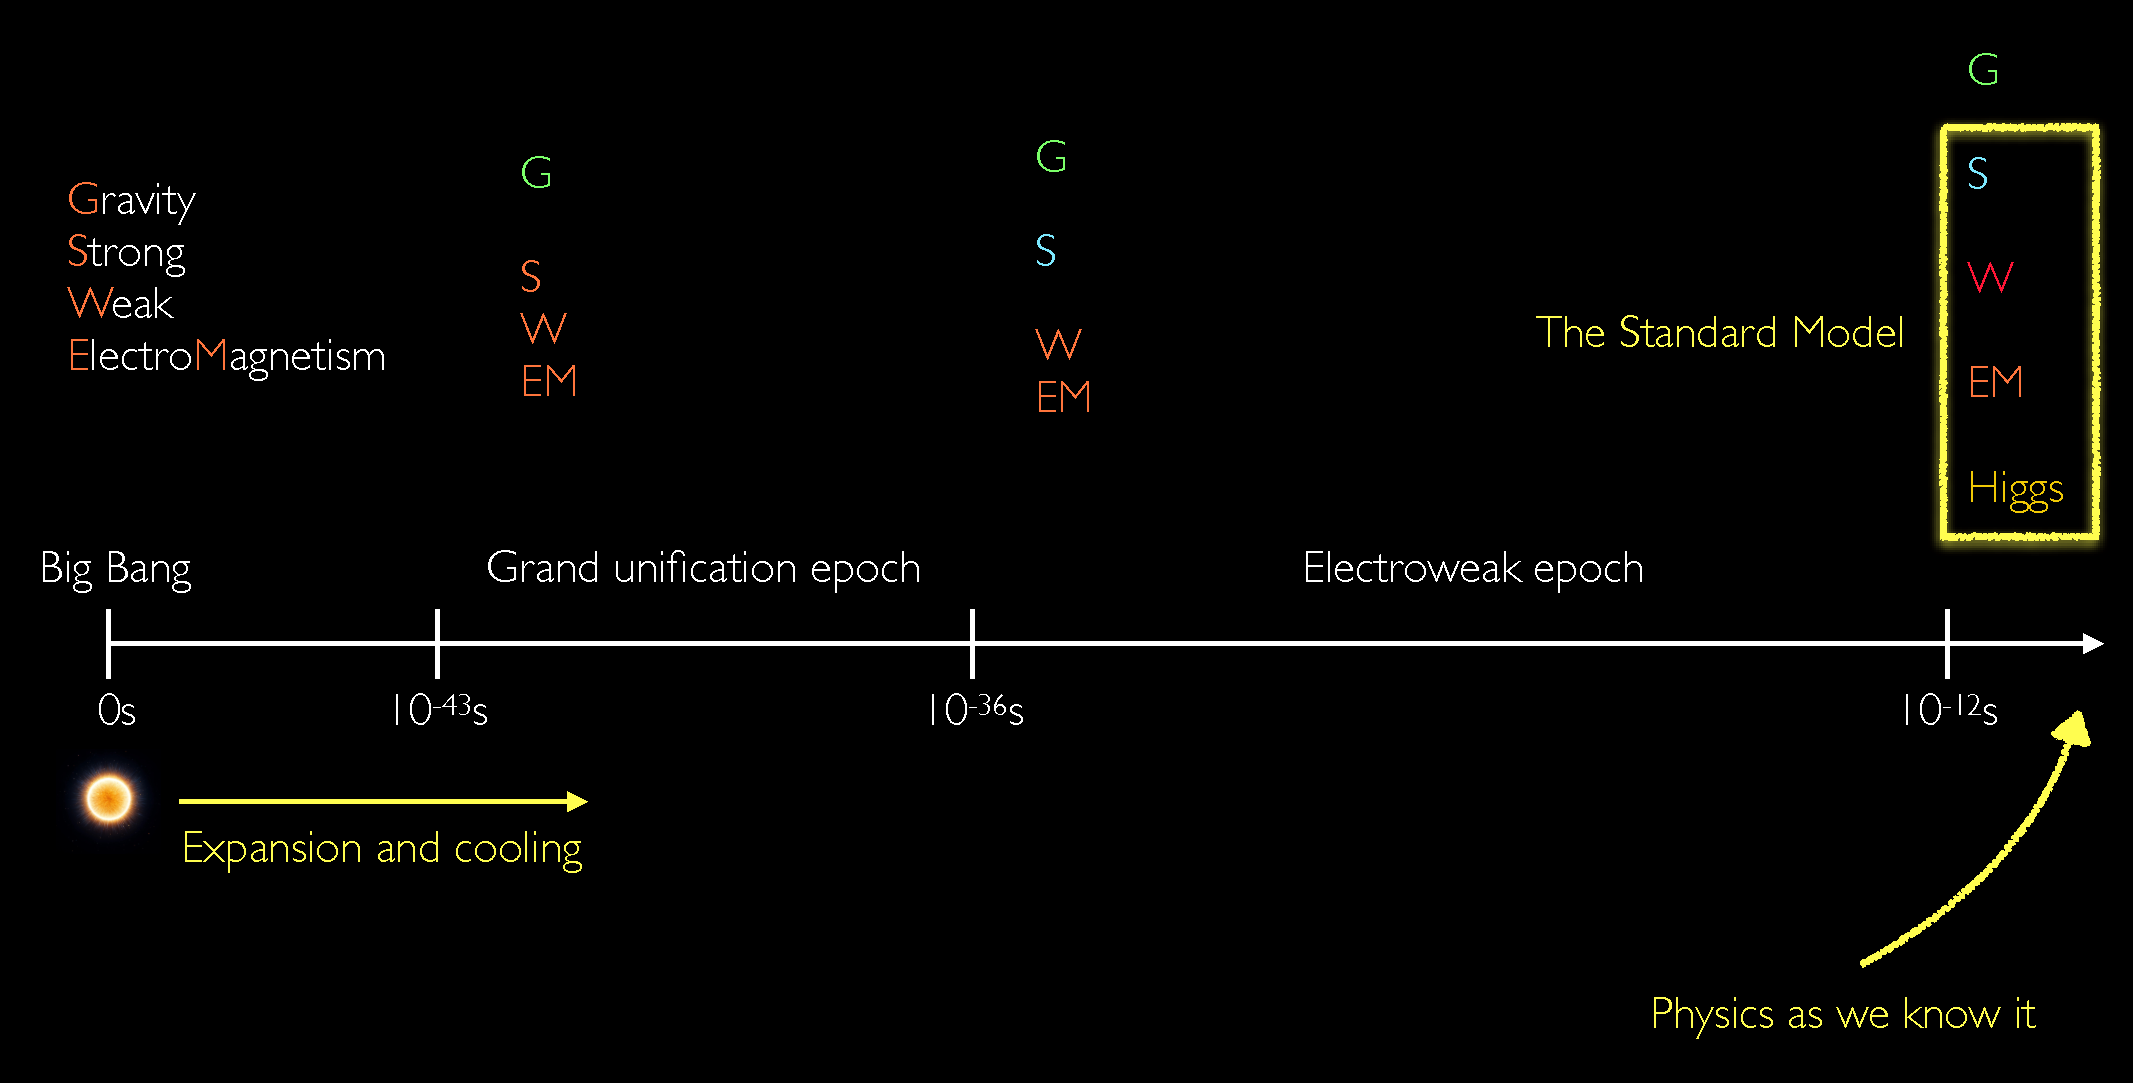
\includegraphics[width=\textwidth]{figures/00-Intro/universe_timeline.pdf}
    \caption{The timeline and evolution of forces in the early universe.}
    \label{fig:00_timeline}
\end{figure}

The universe started with a bang.
A massive burst of energy, temperature, and pressure, with all four fundamental forces --- electromagnetism, nuclear weak, nuclear strong, and gravity --- as one.
Immediately after, the universe expanded and cooled, and after about $10^{-43}$ seconds, gravity parted ways.
$10^{-36}$s later, the strong force separated as well and finally, by around $10^{-12}$s, so did the weak and electromagnetic forces,``turning on'' the Higgs field in the process and leaving us with the fundamental forces and laws of physics as we know them today (Figure~\ref{fig:00_timeline}).

Electromagnetism, the nuclear weak and strong forces, the Higgs field, and all known elementary particles can be elegantly described by the standard model (SM) of particle physics.
Over the last 60 years, it has proven a monumentally successful theory, both explaining and predicting physical phenomena up to energies produced naturally only within a nanosecond of the Big Bang.
These include the prediction of the Higgs boson 50 years before its discovery, explanations for radioactive decay and the binding of atomic nuclei, and the unification of the electromagnetic and weak forces.
However, despite its triumphs, there remain fundamental mysteries that the SM cannot explain.

The most glaring of these is its reconciliation, or lack thereof, with gravity, for which a quantum, SM-compatible theory has proven elusive.
There is also abundant cosmological evidence of ``dark'' matter and energy, constituting 95\% of the universe and yet finding no justification from the SM.
Other subtle mysteries include the inconsistency between the matter-antimatter \textit{a}symmetry  we observe and the symmetry the SM predicts, the mechanism for neutrino masses, and the origin of flavor.

The work in this dissertation is motivated by the strong possibility of many of the answers being tied to the Higgs boson.
It is our newest discovered and least understood elementary particle, and the unique nature of the Higgs field and its interactions leaves open vast potential for intriguing new physics in this sector.
As electroweak symmetry breaking, i.e., the separation of the weak and electromagnetic forces, is intimately connected to a phase transition of the Higgs field, many theories naturally link this transition with the breaking of the matter-antimatter~\cite{Morrissey_2012} and flavor symmetries~\cite{BAZZOCCHI2005372} as well.
The Higgs boson may also be the connection between the SM and the dark sector~\cite{sym13122406}, while the ``Higgs-Saw''~\cite{Krauss:2013oea} mechanism is a promising explanation for dark energy.
% seesaw~\cite{10.1143/PTP.64.1103}

Predictions of these theories include new, rare, Higgs-like particles and/or minute deviations to the interactions of the Higgs boson from the SM.
However, as many of the phenomena therein would have occurred during the electroweak epoch or earlier (see Figure~\ref{fig:00_timeline}), these effects would manifest only at the highest energies, comparable to that of $<1$ps after the Big Bang.
This dissertation presents two complementary efforts to probe such effects, by (1) searching for new, highly energetic Higgs bosons, and (2) measuring Higgs interactions uniquely sensitive to new, high energy physics.

We do so using the Large Hadron Collider (LHC) at CERN.
The LHC accelerates and collides extremely high-speed protons, producing energies comparable to the early universe just 10ps after the Big Bang.
We observe these collisions with the Compact Muon Solenoid (CMS) experiment, one of four massive detectors at the LHC, and one of the two that discovered the Higgs boson in 2012.
Crucially, we emphasize that, with the exponentially increasing rate of collisions and data at the LHC, the CMS experiment is entering an era of unprecedented potential for scientific discovery.

To fully realize this, however, and maximize the impact of our new data, significant computational innovation is required.
To this end, we also present in this dissertation several novel AI techniques to identify high energy Higgs bosons, accelerate simulations of the CMS detector, and complement traditional data analysis techniques with model-agnostic searches for new physics.
Particular emphasis is placed on the development of physics-informed machine learning (ML) algorithms, which uniquely leverage biases of high energy physics (HEP) data to improve their performance and robustness.
Namely, we introduce the first generative models for \textit{point-cloud} data in HEP, which respect the sparsity and high granularity of detector data, and the first anomaly detection models equivariant to Lorentz transformations.

We also describe significant efforts towards \textit{validating} such AI techniques, which is critical for them to ultimately have an impact in the field.
Specifically, we apply a novel method for calibrating ML algorithms targeting Higgs to vector boson decays, which has proven effective not only for the analyses presented in this dissertation but for the broader CMS physics program as well.
We additionally present several studies and new statistical techniques for evaluating fast simulations.
The combination of these and our new AI models has the potential to revolutionize the computing paradigm in CMS, improving the computational efficiency of our simulations by up to three orders of magnitude, and ensuring trust in their modeling of the underlying physics.


This dissertation is organized as follows.
Part~\ref{part:sm} introduces the theoretical basis for this dissertation, starting with the mathematical framework behind symmetries in physics (Chapter~\ref{sec:01_symmetries}) and of quantum field theory (Chapter~\ref{sec:01_qft}) before detailing the SM of particle physics (Chapter~\ref{sec:01_sm}).
Part~\ref{part:epp} then describes the experimental apparatus used in this dissertation: the LHC (Chapter~\ref{sec:02_lhc}) and the CMS experiment (Chapter~\ref{sec:02_cms}).
Part~\ref{part:aiml} concludes the background material with an introduction to ML in HEP (Chapter~\ref{sec:03_ml}), as well as the data analysis and statistical framework used in this dissertation (Chapter~\ref{sec:03_stats}).


Parts~\ref{part:ml4sim}---\ref{part:ml4jets} comprise the novel contributions of this dissertation.
Part~\ref{part:ml4sim} presents new methods for producing and validating fast simulations of the CMS detector using ML, which will be critical to maximizing the scientific output of the LHC in the coming decade.
These methods leverage advancements in generative modeling to develop novel, physics-informed simulation techniques that are orders of magnitude faster than traditional methods.
We also discuss new techniques for robust evaluation of such fast simulation techniques, and the outlook for their use in CMS.

Part~\ref{part:hh} then presents two novel searches to understand the high energy Higgs sector of the SM, targeting the production of Lorentz-boosted Higgs boson pairs, which decay into two beauty quarks and two vector bosons.
Such searches are critical to understanding the properties of the Higgs boson and searching for the effects of new physics at very high energies.
We discuss the analysis techniques used in these searches, particularly the use of deep transformer networks to identify Higgs-boson decays to two vector bosons for the first time, and competitive constraints achieved on new physics models and the two-Higgs-two-vector-boson coupling.

Finally, Part~\ref{part:ml4jets} outlines the development of new software to facilitate research in ML and HEP and ML techniques that respect the symmetries of the high energy collisions that we study.
Namely, we introduce the \jetnet Python package, which has proven impactful in this field, and a novel ML algorithm for searching for new physics while remaining robust to Lorentz-transformations of our data.

\else
    \begin{acknowledgements}
        % Your fancy acks here. Keep in mind you need to ack each paper you
% use. See the examples here. In addition, each chapter ack needs to
% be repeated at the end of the relevant chapter.
\begin{acknowledgements}

% I was in the 10th grade when the Higgs boson was discovered at the CERN Large Hadron Collider.
% Around the same time, I read the \textit{The Universe in a Nutshell} by Stephen Hawking.
% These two events inspired an excitement and thirst to understand our universe that has led me 


% \begin{center}
% 	\parbox{.8\linewidth}{%
% 		\centering
% 		\noindent
% 		\textit{\sout{Football} Physics is the most important of all the least important things in life. --- Jurgen Klopp} --- Javier Duarte
% 	}
% \end{center}

My interest in physics was ignited in the 10th grade by the discovery of the Higgs boson and Stephen Hawking's \textit{The Universe in a Nutshell}. 
These past five years, dedicated to understanding the Higgs and the mysteries of our early universe, have been a fulfillment of dreams then born and will be a part of my life I cherish forever.

I have many people to thank for allowing my childhood passion to flourish into this dissertation.
I start first and foremost with my parents and little Kli for their love and support at every step.
I thank as well my entire extended family for making me feel at home around the world, from Delhi to Pondicherry and California to Texas.
I am especially grateful to all my grandparents, whose wisdom, selflessness, and memory inspire me always.

I would not have survived this PhD --- particularly the two long years of lockdown and two long quarters of E\&M, without my amazing friends, old and new, in San Diego: Aneesh, Biswa, Chris, Davide, Dro, Elliot, Gerald, Hulk, and Varun (to name a few).
I thank as well my fellow CMS students, Farouk and Yanxi, with whom I moved across continents and conducted an ancillary PhD in ping pong.
Along with them, I thank my friends in Geneva and Chicago, including Fifi, Jay, Priyanka, and the LPC crew, for making my two years working at CERN and Fermilab so memorable.
Most of all, I thank Praniti, for her sweetness and support throughout.

Like the universe, my journey in high energy physics (HEP) began with a bang: the CERN Openlab summer student program.
It was a breathtaking experience, and I am grateful to Cliff, Frank, and my supervisor Maurizio for their support then and throughout my career since.
Maurizio, in particular, introduced me to the (Nobel-prize winning!) potential of AI in HEP, and I have been hooked ever since.

More importantly, he introduced me to Javier right as we were both, perhaps serendipitously, joining UCSD in the Fall of 2019.
Javier has been the most brilliant, kind, and supportive advisor I could have asked for, and I thank him for teaching me a lot more than just physics.
Along with him, I thank many awesome postdocs and scientists, including Cristina, Daniel, Nhan, Petar, and Si for their mentorship through the years.

%  for reasons too numerous to list here fully, but I will try to name a few:
% visiting CERN, living in San Diego, living in Geneva, living in Chicago, working at the forefront of AI, pushing our understanding of the Higgs, searching for new particles, making friends with some of the sweetest and most brilliant people in the world, and the most important one of them all, meeting the P\&SGW.

% I have so many people to thank for pushing this interest and letting it flourish into this dissertation, 
% starting first and foremost with my parents for supporting me, my education, and this dream in every way possible.
% It was announced first by Joe Incandela in one of the most groundbreaking seminars of the 21st century.
% Imagine my surprise when he walked into my office at CERN - well, his office really - in the spring of last year and had lunch with my officemates and me.

% It has been a dream and privilege to study this new particle 

\

Parts~\ref{part:sm}---\ref{part:aiml} are primarily original work for this dissertation, discussing the standard model, the CMS experiment and the LHC, AI and ML, and statistics, and building on several references listed therein.
% Chapters 1 and 2 \TODO{...}.
% Chapter~\ref{sec:03_stats} builds on Refs.~\cite{Cowan:2010js,Cranmer:2014lly}.
On the topic of statistics, I thank Javier and Nick Smith for countless discussions (as well as their much-needed help with analysis software and the CMS combine tool)!

Part~\ref{part:ml4sim} presents novel methods for producing and validating fast simulations of the CMS detector using AI.
I thank Maurizio for introducing me to this topic as a summer student and his guidance since, and Javier for supporting this work, and all the research directions it bloomed, since the beginning of my PhD.
I also thank my fellow students on the topic, Mary and Breno; Nadya for her support during my time at CERN; Kevin Pedro for lending his expertise on CMS simulations; and the IRIS-HEP institute and the Fermilab LPC for supporting this work through the IRIS-HEP fellowship and the LPC AI fellowship and graduate scholarship, respectively.

Part~\ref{part:hh} describes searches for high energy Higgs-boson pair production in the \bbvv channel using data collected by the CMS experiment during Run 2 of the LHC.
I thank Cristina for her hands-on guidance on both the physics and technical aspects from the start and her patience as I refactored our codebase every week.
I thank as well Javier, Petar, Si, and the rest of our boosted double-Higgs working group, as well as Nhan and the DASZLE team, for their advice and support.
I thank finally Nick, Lindsey, and all the Coffea and Scikit-HEP developers for building a wonderful and supportive Pythonic HEP ecosystem.
% allowing me to complete a PhD in HEP without using ROOT.

Part~\ref{part:ml4jets} on the \jetnet library and Lorentz-equivariant ML represents a collection of work~\cite{Kansal:2023iqy, Tsan:2021brw, Hao:2022zns} on which I mentored some amazing students at UC San Diego and more.
I thank them all
% ---
% Andres,
% Anni,
% Carlos,
% Krish,
% Rounak,
% Saloni,
% Tina,
% Venkat,
% Zichun,
% Zhaoyu (Tina),
% and the ENLACE team
% ---
for choosing me as their mentor, and Javier for encouraging and supporting us graduate students in engaging in so many rewarding mentorship opportunities. 

\

Chapter~\ref{sec:03_ml} is, in part, a reprint of the materials as they appear in
R. Kansal. ``Symmetry Group Equivariant Neural Networks,'' (2020);
and
NeurIPS, 2021, R. Kansal; J. Duarte; H. Su; B. Orzari; T. Tomei; M. Pierini; M. Touranakou; J.-R. Vlimant; and D. Gunopulos. Particle Cloud Generation with Message Passing Generative Adversarial Networks.
The dissertation author was the primary investigator and author of these papers.

Part~\ref{part:ml4sim} is, in part, a reprint of the materials as they appear in 
the NeurIPS ML4PS Workshop, 2020, R. Kansal; J. Duarte; B. Orzari; T. Tomei; M. Pierini; M. Touranakou; J.-R. Vlimant; and D. Gunopulos. Graph generative adversarial networks for sparse data generation in high energy physics;
NeurIPS, 2021, R. Kansal; J. Duarte; H. Su; B. Orzari; T. Tomei; M. Pierini; M. Touranakou; J.-R. Vlimant; and D. Gunopulos. Particle Cloud Generation with Message Passing Generative Adversarial Networks; and
Phys. Rev. D, 2023, R. Kansal; A. Li; J. Duarte; N. Chernyavskaya; M. Pierini; B. Orzari; and T. Tomei; Evaluating generative models in high energy physics; and
the NeurIPS ML4PS Workshop, 2024, A. Li; V. Krishnamohan; R. Kansal; J. Duarte; R. Sen; S. Tsan; and Z. Zhang; Induced generative adversarial particle transformers.
The dissertation author was the primary investigator and (co-)author of these papers.

Chapters~\ref{sec:05_smhh} and~\ref{sec:05_bsmxhy} and Part~\ref{part:hh}, in part, are currently being prepared for the publication of the material by the CMS collaboration.
The dissertation author was the primary investigator and author of these papers.

Part~\ref{part:ml4jets} is, in part, a reprint of the materials as they appear in
JOSS, 2023, R. Kansal; C. Pareja; Z. Hao; and J. Duarte; JetNet: A Python package for accessing open datasets and benchmarking machine learning methods in high energy physics; and
Eur. Phys. J. C, 2023, Z. Hao; R. Kansal; J. Duarte; and N. Chernyavskaya; Lorentz group equivariant autoencoders.
%  and
% the NeurIPS ML4PS Workshop, 2021, S. Tsan; R. Kansal; A. Aportela; D. Diaz; J. Duarte; S. Krishna; F. Mokhtar; J.-R. Vlimant; and M. Pierini; Particle graph autoencoders and differentiable, learned energy mover's distance;
The dissertation author was the primary investigator and (co-)author of these papers.

\end{acknowledgements}
    \end{acknowledgements}

    \begin{vita}
        \noindent
\begin{cv}{}
\begin{cvlist}{}
\item[2019] Bachelor of Science in Physics and Computer Engineering\\
            University of California San Diego\\
            \textit{Summa cum laude}
\item[2019] CERN Openlab Summer Student
\item[2019] IRIS-HEP Fellow
\item[2019-2024] Graduate Student Researcher\\University of California San Diego
\item[2021-2022] Artificial Intelligence Fellow\\Fermilab LHC Physics Center
\item[2023-2024] Graduate Scholar\\Fermilab LHC Physics Center
\item[2024] Doctor of Philosophy in Physics\\University of California San Diego
\item[2024-] AI/Schmidt Postdoctoral Scholar Research Associate\\California Institute of Technology and Fermilab
\end{cvlist}
\end{cv}

% \clearpage
\publications

\noindent
\textit{Note: as a member of the CMS collaboration, I have been an author on all CMS papers since 2019. 
The following includes only the CMS publications to which I made significant contributions during my PhD.}
\\[0.1\baselineskip]
\begin{enumerate}[itemsep=\baselineskip]
    \item CMS Collaboration, “Search for Nonresonant Pair Production of Highly Energetic Higgs Bosons Decaying to Bottom Quarks and Vector Bosons”, in prep, CMS-HIG-23-012 (2023).
    \item CMS Collaboration, “Search for a massive scalar resonance decaying to a light scalar and a Higgs boson in the two b quarks and four light quarks final state”, in prep, CMS-B2G-23-007 (2023).
    \item A. Li*, V. Krishnamohan*, \textcolor{authorhighlight}{R. Kansal}, J. Duarte, R. Sen, S. Tsan, and Z. Zhang, “Induced generative adversarial particle transformers”, NeurIPS ML4PS Workshop (2023), \href{https://arxiv.org/abs/2312.04757}{arXiv:2312.04757}.
    \item \textcolor{authorhighlight}{R. Kansal}, C. Pareja, Z. Hao, and J. Duarte, “JetNet: A Python package for accessing open datasets and benchmarking machine learning methods in high energy physics”, \href{https://doi.org/10.21105/joss.05789}{\textbf{JOSS} 8, 5789} (2023).
    \item Z. Hao, \textcolor{authorhighlight}{R. Kansal}, J. Duarte, and N. Chernyavskaya, “Lorentz group equivariant autoencoders”, \href{https://doi.org/10.1140/epjc/s10052-023-11633-5}{\textbf{Eur. Phys. J. C} 83, 485} (2023), \href{https://arxiv.org/abs/2212.07347}{arXiv:2212.07347}.
    \item \textcolor{authorhighlight}{R. Kansal}, A. Li, J. Duarte, N. Chernyavskaya, M. Pierini, B. Orzari, and T. Tomei, “Evaluating generative models in high energy physics”, \href{https://doi.org/10.1103/PhysRevD.107.076017}{\textbf{Phys. Rev. D} 107, 076017} (2023), \href{https://arxiv.org/abs/2211.10295}{arXiv:2211.10295}.
    \item CMS Collaboration, “Search for Nonresonant Pair Production of Highly Energetic Higgs Bosons Decaying to Bottom Quarks”, \href{https://doi.org/10.1103/PhysRevLett.131.041803}{\textbf{Phys. Rev. Lett.} 131, 041803} (2023), \href{https://arxiv.org/abs/2205.06667}{arXiv:2205.06667}.
    \item \textcolor{authorhighlight}{R. Kansal}, J. Duarte, H. Su, B. Orzari, T. Tomei, M. Pierini, M. Touranakou, J.-R. Vlimant, and D. Gunopulos, “Particle Cloud Generation with Message Passing Generative Adversarial Networks”, NeurIPS (2021), \href{https://arxiv.org/abs/2106.11535}{arXiv:2106.11535}.
    \item F. Mokhtar, \textcolor{authorhighlight}{R. Kansal}, and J. Duarte, “Do graph neural networks learn traditional jet substructure?”, NeurIPS ML4PS Workshop (2022), \href{https://arxiv.org/abs/2211.09912}{arXiv:2211.09912}.
    \item M. Touranakou, N. Chernyavskaya, J. Duarte, D. Gunopulos, \textcolor{authorhighlight}{R. Kansal}, B. Orzari, M. Pierini, T. Tomei, and J.-R. Vlimant, “Particle-based fast jet simulation at the LHC with variational autoencoders”, \href{https://doi.org/10.1088/2632-2153/ac7c56}{\textbf{Machine Learning: Science and Technology} 3, 035003} (2022), \href{https://arxiv.org/abs/2203.00520}{arXiv:2203.00520}.
    \item A. Apresyan, D. Diaz, J. Duarte, S. Ganguly, \textcolor{authorhighlight}{R. Kansal}, N. Lu, C. M. Suarez, S. Mukherjee, C. Peña, B. Sheldon, and S. Xie, “Improving Di-Higgs Sensitivity at Future Colliders in Hadronic Final States with Machine Learning”, Contribution to Snowmass Summer Study (2022), \href{https://arxiv.org/abs/2203.07353}{arXiv:2203.07353}.
    \item Y. Chen et al., “A FAIR and AI-ready Higgs boson decay dataset”, \href{https://doi.org/10.1038/s41597-021-01109-0}{\textbf{Sci. Data} 9, 31} (2021), \href{https://arxiv.org/abs/2108.02214}{arXiv:2108.02214}.
    \item F. Mokhtar, \textcolor{authorhighlight}{R. Kansal}, D. Diaz, J. Duarte, J. Pata, M. Pierini, and J.-R. Vlimant, “Explaining machine-learned particle-flow reconstruction”, NeurIPS ML4PS Workshop (2021), \href{https://arxiv.org/abs/2111.12840}{arXiv:2111.12840}.
    \item S. Tsan, \textcolor{authorhighlight}{R. Kansal}, A. Aportela, D. Diaz, J. Duarte, S. Krishna, F. Mokhtar, J.-R. Vlimant, and M. Pierini, “Particle graph autoencoders and differentiable, learned energy mover’s distance”, NeurIPS ML4PS Workshop (2021), \href{https://arxiv.org/abs/2111.12849}{arXiv:2111.12849}.
    \item B. Orzari, T. Tomei, M. Pierini, M. Touranakou, J. Duarte, \textcolor{authorhighlight}{R. Kansal}, J.-R. Vlimant, and D. Gunopulos, “Sparse Data Generation for Particle-Based Simulation of Hadronic Jets in the LHC”, ICML LXAI Workshop (2021), \href{https://arxiv.org/abs/2109.15197}{arXiv:2109.15197}.
    \item \textcolor{authorhighlight}{R. Kansal}, J. Duarte, B. Orzari, T. Tomei, M. Pierini, M. Touranakou, J.-R. Vlimant, and D. Gunopulos, “Graph generative adversarial networks for sparse data generation in high energy physics”, NeurIPS ML4PS Workshop (2020), \href{https://arxiv.org/abs/2012.00173}{arXiv:2012.00173}.
\end{enumerate}
    \end{vita}

    \begin{dissertationabstract}
        This dissertation describes efforts towards understanding the Higgs boson at the highest energies humanly accessible, using the CMS experiment at the Large Hadron Collider and advances in artificial intelligence (AI) and machine learning (ML).
We present searches for resonant and nonresonant Higgs-boson (\PH) pair production in the all-hadronic two beauty-quark and two vector boson (\PV) final state, using a novel strategy to measure the quartic \HHVV coupling and search for new Higgs-like bosons.
By targeting highly Lorentz-boosted Higgs pairs, we probe effects of potential new physics in the high energy Higgs sector, which could hold answers to fundamental mysteries of nature such as baryon asymmetry.

To enable these and future searches, we introduce as well significant developments in AI/ML, including in the identification of boosted \hvv decays with deep transformer networks and advances in AI-accelerated fast simulations of the CMS detector.
The latter notably includes the development of the first, highly performant generative models for point-cloud data in high energy physics, which have the potential to improve CMS' computational efficiency by up to three orders of magnitude.
We also highlight novel solutions to the important and challenging problems of calibrating and validating these ML techniques.
Finally, we present new approaches to search for new physics in a model-agnostic manner, using physics-informed ML methods equivariant to Lorentz transformations.

The quartic \HHVV coupling is observed (expected) to be constrained to $[-0.04, 2.05]$ ($[0.05, 1.98]$) at the 95\% confidence level relative to the standard model prediction, representing the second-most sensitive measurement of this coupling by CMS to date.
Exclusion limits on the production cross section of new heavy resonances decaying to two Higgs-like bosons are expected to be as low as 0.3\unit{fb} for high resonance masses.
    \end{dissertationabstract}

    \mainmatter

    \begin{dissertationintroduction}
        \label{sec:intro}

\begin{center}
    \centering
    \noindent
    \textit{The story so far:
    In the beginning the Universe was created.
    This has made a lot of people very angry and been widely regarded as a bad move.
    }
    \vskip0.2\baselineskip
    - Douglas Adams, The Restaurant at the End of the Universe
\end{center}

\vskip0.5\baselineskip

\begin{figure}[h!]
    \centering
    \captionsetup{justification=centering}
    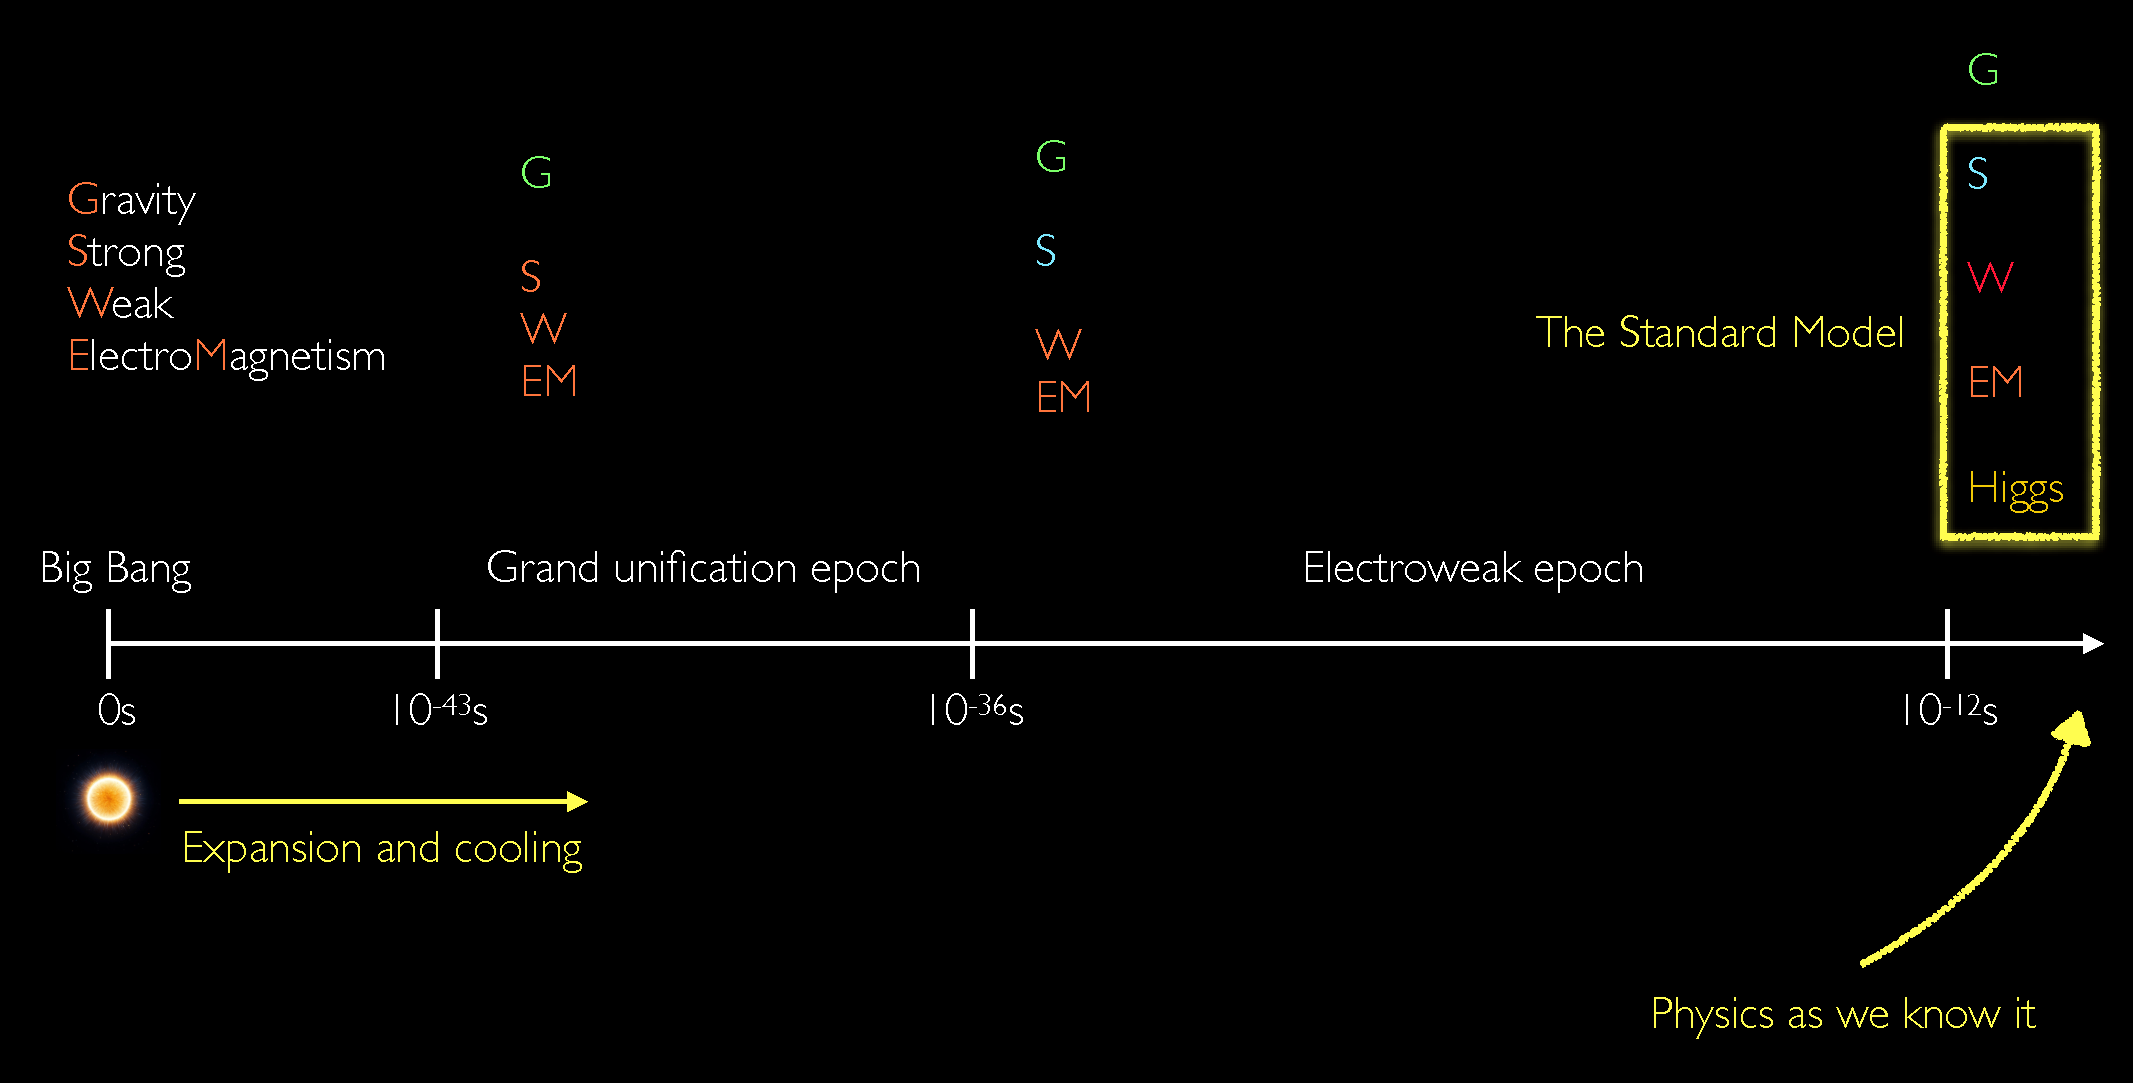
\includegraphics[width=\textwidth]{figures/00-Intro/universe_timeline.pdf}
    \caption{The timeline and evolution of forces in the early universe.}
    \label{fig:00_timeline}
\end{figure}

The universe started with a bang.
A massive burst of energy, temperature, and pressure, with all four fundamental forces --- electromagnetism, nuclear weak, nuclear strong, and gravity --- as one.
Immediately after, the universe expanded and cooled, and after about $10^{-43}$ seconds, gravity parted ways.
$10^{-36}$s later, the strong force separated as well and finally, by around $10^{-12}$s, so did the weak and electromagnetic forces,``turning on'' the Higgs field in the process and leaving us with the fundamental forces and laws of physics as we know them today (Figure~\ref{fig:00_timeline}).

Electromagnetism, the nuclear weak and strong forces, the Higgs field, and all known elementary particles can be elegantly described by the standard model (SM) of particle physics.
Over the last 60 years, it has proven a monumentally successful theory, both explaining and predicting physical phenomena up to energies produced naturally only within a nanosecond of the Big Bang.
These include the prediction of the Higgs boson 50 years before its discovery, explanations for radioactive decay and the binding of atomic nuclei, and the unification of the electromagnetic and weak forces.
However, despite its triumphs, there remain fundamental mysteries that the SM cannot explain.

The most glaring of these is its reconciliation, or lack thereof, with gravity, for which a quantum, SM-compatible theory has proven elusive.
There is also abundant cosmological evidence of ``dark'' matter and energy, constituting 95\% of the universe and yet finding no justification from the SM.
Other subtle mysteries include the inconsistency between the matter-antimatter \textit{a}symmetry  we observe and the symmetry the SM predicts, the mechanism for neutrino masses, and the origin of flavor.

The work in this dissertation is motivated by the strong possibility of many of the answers being tied to the Higgs boson.
It is our newest discovered and least understood elementary particle, and the unique nature of the Higgs field and its interactions leaves open vast potential for intriguing new physics in this sector.
As electroweak symmetry breaking, i.e., the separation of the weak and electromagnetic forces, is intimately connected to a phase transition of the Higgs field, many theories naturally link this transition with the breaking of the matter-antimatter~\cite{Morrissey_2012} and flavor symmetries~\cite{BAZZOCCHI2005372} as well.
The Higgs boson may also be the connection between the SM and the dark sector~\cite{sym13122406}, while the ``Higgs-Saw''~\cite{Krauss:2013oea} mechanism is a promising explanation for dark energy.
% seesaw~\cite{10.1143/PTP.64.1103}

Predictions of these theories include new, rare, Higgs-like particles and/or minute deviations to the interactions of the Higgs boson from the SM.
However, as many of the phenomena therein would have occurred during the electroweak epoch or earlier (see Figure~\ref{fig:00_timeline}), these effects would manifest only at the highest energies, comparable to that of $<1$ps after the Big Bang.
This dissertation presents two complementary efforts to probe such effects, by (1) searching for new, highly energetic Higgs bosons, and (2) measuring Higgs interactions uniquely sensitive to new, high energy physics.

We do so using the Large Hadron Collider (LHC) at CERN.
The LHC accelerates and collides extremely high-speed protons, producing energies comparable to the early universe just 10ps after the Big Bang.
We observe these collisions with the Compact Muon Solenoid (CMS) experiment, one of four massive detectors at the LHC, and one of the two that discovered the Higgs boson in 2012.
Crucially, we emphasize that, with the exponentially increasing rate of collisions and data at the LHC, the CMS experiment is entering an era of unprecedented potential for scientific discovery.

To fully realize this, however, and maximize the impact of our new data, significant computational innovation is required.
To this end, we also present in this dissertation several novel AI techniques to identify high energy Higgs bosons, accelerate simulations of the CMS detector, and complement traditional data analysis techniques with model-agnostic searches for new physics.
Particular emphasis is placed on the development of physics-informed machine learning (ML) algorithms, which uniquely leverage biases of high energy physics (HEP) data to improve their performance and robustness.
Namely, we introduce the first generative models for \textit{point-cloud} data in HEP, which respect the sparsity and high granularity of detector data, and the first anomaly detection models equivariant to Lorentz transformations.

We also describe significant efforts towards \textit{validating} such AI techniques, which is critical for them to ultimately have an impact in the field.
Specifically, we apply a novel method for calibrating ML algorithms targeting Higgs to vector boson decays, which has proven effective not only for the analyses presented in this dissertation but for the broader CMS physics program as well.
We additionally present several studies and new statistical techniques for evaluating fast simulations.
The combination of these and our new AI models has the potential to revolutionize the computing paradigm in CMS, improving the computational efficiency of our simulations by up to three orders of magnitude, and ensuring trust in their modeling of the underlying physics.


This dissertation is organized as follows.
Part~\ref{part:sm} introduces the theoretical basis for this dissertation, starting with the mathematical framework behind symmetries in physics (Chapter~\ref{sec:01_symmetries}) and of quantum field theory (Chapter~\ref{sec:01_qft}) before detailing the SM of particle physics (Chapter~\ref{sec:01_sm}).
Part~\ref{part:epp} then describes the experimental apparatus used in this dissertation: the LHC (Chapter~\ref{sec:02_lhc}) and the CMS experiment (Chapter~\ref{sec:02_cms}).
Part~\ref{part:aiml} concludes the background material with an introduction to ML in HEP (Chapter~\ref{sec:03_ml}), as well as the data analysis and statistical framework used in this dissertation (Chapter~\ref{sec:03_stats}).


Parts~\ref{part:ml4sim}---\ref{part:ml4jets} comprise the novel contributions of this dissertation.
Part~\ref{part:ml4sim} presents new methods for producing and validating fast simulations of the CMS detector using ML, which will be critical to maximizing the scientific output of the LHC in the coming decade.
These methods leverage advancements in generative modeling to develop novel, physics-informed simulation techniques that are orders of magnitude faster than traditional methods.
We also discuss new techniques for robust evaluation of such fast simulation techniques, and the outlook for their use in CMS.

Part~\ref{part:hh} then presents two novel searches to understand the high energy Higgs sector of the SM, targeting the production of Lorentz-boosted Higgs boson pairs, which decay into two beauty quarks and two vector bosons.
Such searches are critical to understanding the properties of the Higgs boson and searching for the effects of new physics at very high energies.
We discuss the analysis techniques used in these searches, particularly the use of deep transformer networks to identify Higgs-boson decays to two vector bosons for the first time, and competitive constraints achieved on new physics models and the two-Higgs-two-vector-boson coupling.

Finally, Part~\ref{part:ml4jets} outlines the development of new software to facilitate research in ML and HEP and ML techniques that respect the symmetries of the high energy collisions that we study.
Namely, we introduce the \jetnet Python package, which has proven impactful in this field, and a novel ML algorithm for searching for new physics while remaining robust to Lorentz-transformations of our data.

    \end{dissertationintroduction}
\fi

% \part{Theoretical Background}
% \label{part:sm}

% % \chapter{The Standard Model}
% \label{sec:01_sm}

\chapter{Introduction to the Standard Model}
\label{sec:01_intro}

\begin{center}
	\centering
	\noindent
	\textit{God used beautiful mathematics in creating the world.} --- Paul Dirac~\cite{pagels2012cosmic}
\end{center}

\vskip0.5\baselineskip

The standard model (SM) of particle physics is perhaps the greatest scientific theory of all time.
It is a mathematical representation of three fundamental forces, all known elementary particles, and their collective interactions.
In a broader sense, it is also the culmination of centuries of iterative, syncretic experimental results and theoretical advances, from Newton's laws of motion up to the discovery of the Higgs boson.
That such a wide array of seemingly idiosyncratic physical phenomena and theories --- electricity, magnetism, radioactive decays, quantum mechanics, special relativity, the structure of the atom, the binding of the nucleus, the behavior of elementary particles, and more --- can all be encapsulated at their most primordial level into a single theory exemplifies the beauty of the SM.
% In this chapter, we
% Indeed, on a personal note, this is what has always attracted me to particle physics, and I attempt in this chapter to capture just some of the beauty of the SM.

This beauty is perhaps most apparent when viewing the SM through the lens of \textit{symmetries}.
Symmetries provide an elegant way to precisely describe the extremely complex physics mentioned above.
Indeed, superficially, the SM can be viewed simply as a classification of elementary particles and their interactions according to their behavior under different symmetries of the universe and its mathematical description.

This is illustrated in Figure~\ref{fig:01_sm}, listing the SM particles and their properties.
They are first divided into two classes, fermions and bosons, based on how they behave under Lorentz transformations --- a fundamental physical symmetry of nature.
This simple distinction has profound implications: fermions constitute matter, i.e. what all the ``stuff'' in the universe is made out of, while bosons are the particles responsible for forces and their interactions.
Specifically, the photon mediates electromagnetism, the $W^{\pm}$ and $Z$ bosons the weak force, and gluons the strong force.
There is also the Higgs boson, which is special: it does not mediate a force in the classical sense, but its interactions with elementary particles are what imbues them with mass.

\begin{figure}[ht!]
	\centering
	% \captionsetup{justification=centering}
	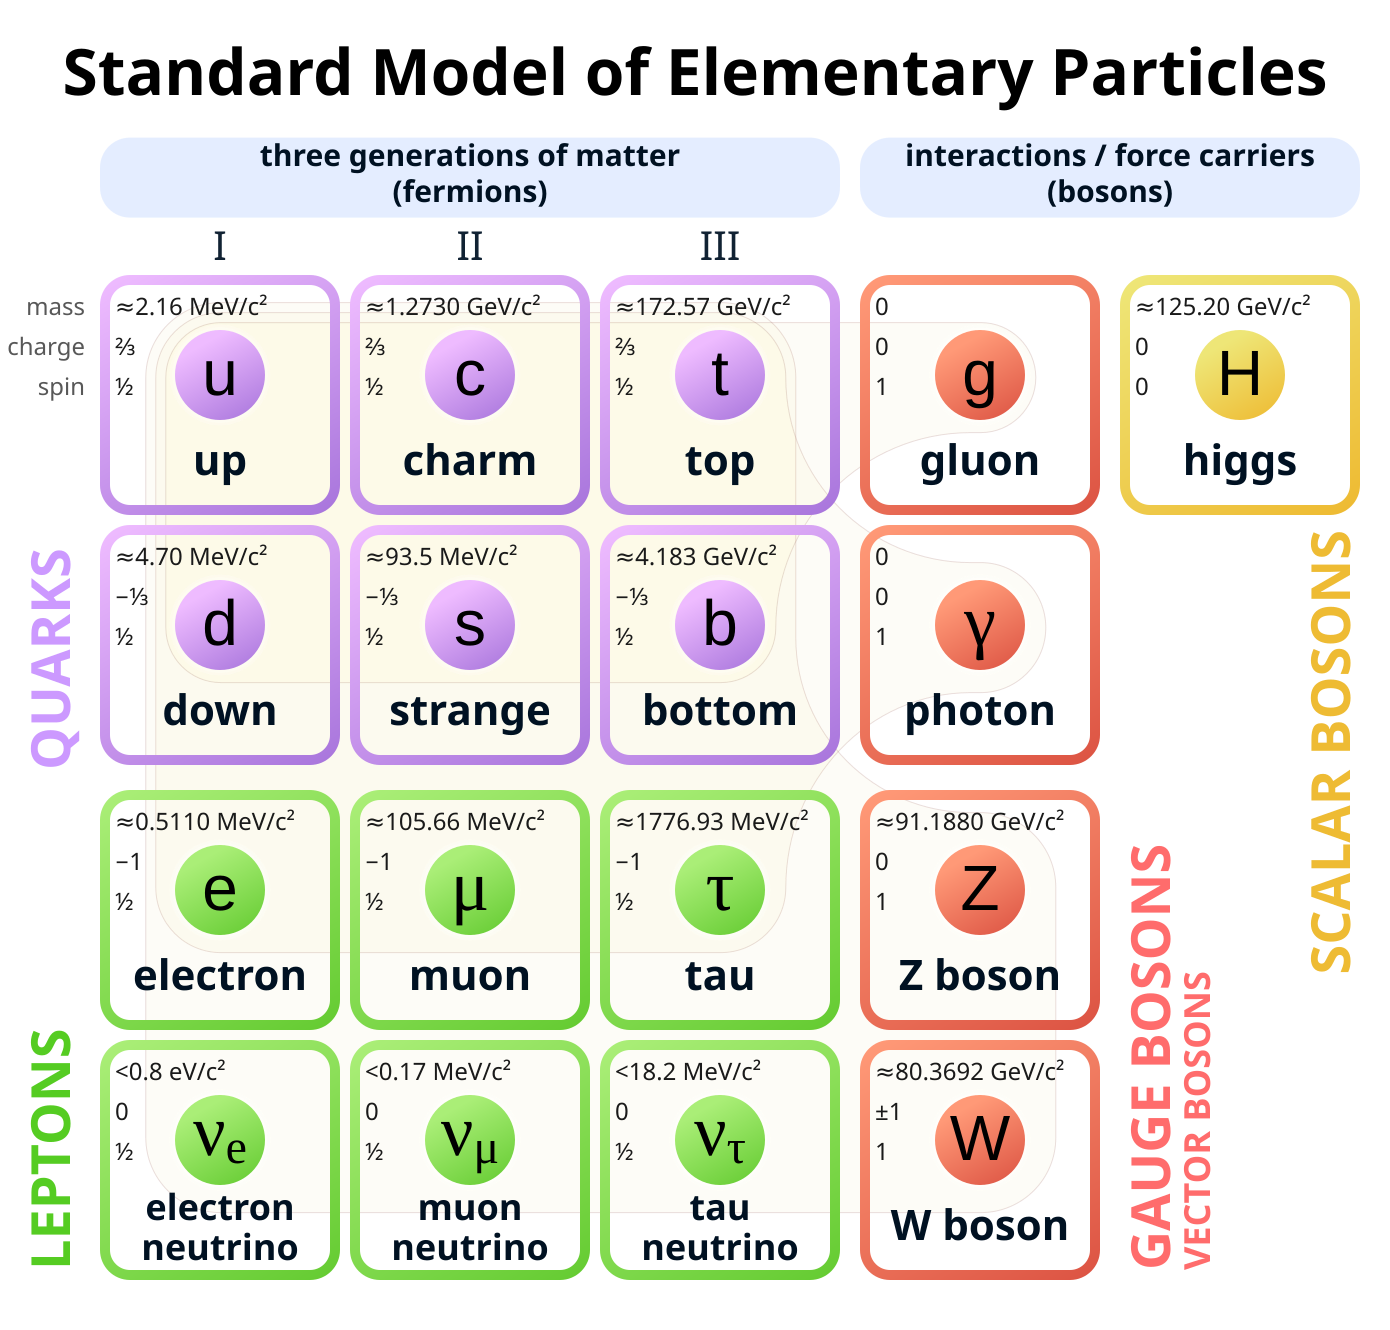
\includegraphics[width=0.8\textwidth]{figures/01-SM/sm_diagram.png}
	\caption{Particles and their classifications in the SM, reproduced from Ref.~\cite{enwiki:1238968997}.}
	\label{fig:01_sm}
\end{figure}

Each force is intimately tied to a symmetry in the SM, and particles are further distinguished by their behavior under these symmetries --- or, equivalently, how they are affected by this force.
Fermions are divided by those interacting (quarks) and not interacting (leptons) with the nuclear strong force, while each of their rows in Figure~\ref{fig:01_sm} further separates them by different ``charges'' under the weak force.
Additionally, each particle's mass and electric charge represent the strength of its interaction with the Higgs and electromagnetic fields, respectively.
Finally, we can see a mysterious \textit{almost}-symmetry: there are three copies, or ``flavors'' or ``generations'', of each fermion, which are entirely identical but for their masses (e.g. the electron, muon, and tau family of particles).
Such a structure may suggest the presence of new, yet-to-be-discovered forces tied to this symmetry.

The goal of Part~\ref{part:sm} is to make this picture more precise, and lay the theoretical foundation for the work discussed in this dissertation.
The mathematical frameworks needed to do so are called group theory and quantum field theory (QFT), and are the subjects of Chapters~\ref{sec:01_symmetries} and~\ref{sec:01_qft}, respectively.
Equipped with these tools, we then describe the SM in Chapter~\ref{sec:01_sm}, including the interactions discussed above and, of most relevance to the subject of this dissertation, the phenomenon of jets, the Higgs sector, and Higgs boson pair production within and beyond the SM.

These chapters build off of several great resources, including:
\begin{itemize}
	\item David Tong's extremely useful and insightful lecture notes on QFT~\cite{TongQFT}, gauge theories~\cite{TongGT}, and the standard model~\cite{TongSM};
	\item John McGreevy's great course on symmetry in physics~\cite{McGreevyGT} (which I had the pleasure of attending in the Fall of 2020);
	\item Frederic Schuller's precise lectures on the geometric anatomy of theoretical physics~\cite{SchullerGATP};
	\item Tony Zee's \textit{Group Theory in a Nutshell for Physicists}~\cite{Zee:2016fuk} and \textit{Quantum Field Theory in a Nutshell}~\cite{Zee:2003mt};
	\item Peskin and Schroeder's classic \textit{An Introduction to Quantum Field Theory}~\cite{Peskin:1995ev};
	\item Gavin Salam's lectures on \textit{Elements of QCD for hadron colliders}~\cite{Salam:2010zt};
	\item and Hong Liu~\cite{LiuRQFT} and Ricardo Matheus'~\cite{MatheusQFT} clear, recorded lectures on QFT.
\end{itemize}

% 
\chapter{Symmetries in physics}
\label{sec:01_symmetries}

\begin{center}
	\centering
	\noindent
	\textit{Perfectly balanced, as all things should be.} --- Thanos
\end{center}

Symmetry is a powerful and beautiful way to understand nature.
Intuitively, a symmetry is a transformation that leaves an object unchanged.
For example, a plain square has a four-fold rotational symmetry: it looks identical rotated once, twice, thrice, or four times by $90^{\circ}$.

Similarly, in physics, a symmetry is a transformation that leaves the laws of physics unchanged.
Electromagnetism, for example, is invariant to translations in space or time: electric charges and currents should behave the same in San Diego 5 years ago as in Geneva today.
Understanding such symmetries, and accounting for them in our mathematical formulation, has been a guiding principle in the development of the SM over the 20th century, and is one in understanding it as well.

In recent years, symmetries have also guided the development of machine learning algorithms in becoming more powerful and efficient.
A particular focus is placed in this dissertation on such \textit{equivariant} algorithms, which respect the symmetries and
\textit{inductive biases} of our high energy physics data.
This chapter lays the foundation for these ideas, which we discuss in more detail in Chapter~\ref{sec:03_ml} and contribute to in Chapter~\ref{sec:06_lgae}.

In this chapter, we first introduce the framework for describing symmetries, group theory, in Section~\ref{sec:01_symmetries_gt}.
We then describe Lie algebras for continuous symmetries, and derive representations for the algebra corresponding to 3D rotations, in Section~\ref{sec:01_symmetries_so3}.
% in Sections~\ref{sec:01_symmetries_continuous} and~\ref{sec:01_symmetries_lie}, respectively.
% We then derive representations of the Lie algebra corresponding to 3D rotations in Section~\ref{sec:01_symmetries_so3}.
We conclude in Section~\ref{sec:01_symmetries_poincare} with a discussion of the Lorentz and Poincaré groups, comprising the fundamental symmetries of spacetime, whose irreducible representations are what we call particles.
% This  lays the foundations for describing \textit{group-equivariant} machine learning algorithms, an exciting area of research in AI that will be a focus of Chapter~\ref{sec:06_ml4jets}.

\section{Group theory}
\label{sec:01_symmetries_gt}

The mathematical formalism for describing symmetries is called \textit{group theory}.

\begin{definition}
\label{def:01_group}
The fundamental object in group theory is a \textit{group}, defined as a pair $(G, \bullet)$, where $G$ is a set and $\bullet: G \times G \rightarrow G$ is the group operation, which together satisfies the following properties:
\begin{enumerate}[i)]
	\item Associativity: $\forall a, b, c \in G: (a \bullet b) \bullet c = a \bullet (b \bullet c)$.
	\item Identity element: $\exists e \in G: \forall a \in G: a \bullet e = e \bullet a = a$.
	\item Inverse element: $\forall a \in G: \exists a^{-1} \in G: a \bullet a^{-1} = a^{-1} \bullet a = e$.
\end{enumerate}
\end{definition}

\begin{definition}
\label{def:01_abelian}
Note from Definition~\ref{def:01_group} that the group operation is not necessarily commutative ($\forall a, b \in G: a \bullet b = b \bullet a$).
If this condition does hold, the group is called an \textit{abelian} group.
\end{definition}

\begin{example}
\label{example:01_square}
To formalize the four-fold rotation symmetry of a square discussed above, we can define the group $\mathbb Z_4$  as ($\{0, 1, 2, 3\}$, $+_4$), where $+_4$ is addition modulo 4, and the elements of the set can represent rotations by $0^{\circ}$, $90^{\circ}$, $180^{\circ}$, and $270^{\circ}$, respectively.
One can check that $\mathbb Z_4$ satisfies all the properties of an abelian group.
\end{example}

\subsubsection{Group representations}

To make the abstract mathematical structure of the group more concrete, we next consider \textit{representations} of groups.

\begin{definition}
\label{def:01_representation}
A group representation $R$, of dimension $d$, is a mapping of the group elements to $d\times d$ matrices $D(g)$ in some $d$-dimensional vector space $V$, such that the group operation is preserved: $D(g_1)D(g_2) = D(g_1 \bullet g_2)$.
Necessarily, this means that $D(e) = \identity$, the identity matrix of $V$.
Representations of a group are not unique, and arbitrarily many new represenations can be constructed simply by taking tensor sums and products, denoted by the $\oplus$ and $\otimes$ symbols respectively, of existing ones.
\end{definition}

\begin{definition}
\label{def:01_irreps}
An \textit{irreducible representation} (irrep) is one with no non-trivial invariant subspaces, i.e., it cannot be decomposed into the tensor sums of smaller-dimensional representations.\footnote{Technically, certain pathological reducible representations of non-compact groups also cannot be decomposed into irreps, so ``non-decomposability'' is a necessary but insufficient condition for irreps.}
\end{definition}

\begin{example}
\label{example:01_square_representation}
The group $\mathbb Z_4$ from Example~\ref{example:01_square} can be represented simply as scalar complex numbers ($V = \mathbb C$):
\begin{equation}
	\label{eq:01_z4_representation}
	\begin{array}{cccc}
	0 & 1 & 2 & 3 \\
	\downarrow & \downarrow & \downarrow & \downarrow \\
	1 & e^{i\frac{\pi}{2}} & e^{i\pi} & e^{i\frac{3\pi}{2}}
	\end{array}
\end{equation}
One can check this satisfies the conditions of Definition~\ref{def:01_representation}, and since it is 1-dimensional, it is also irreducible.
\end{example}

\begin{definition}
\label{def:01_symmetry_regular_representation}
Every group has a $|G|$-dimensional \textit{regular representation} $R^{\mathrm{reg}}$, where $|G|$ is the number elements of the group, called the \textit{order} of the group.
The vector space $V = \mathrm{span}\{\ket{g}|g\in G\}$, and the representation is defined such that
\begin{equation}
	\label{eq:01_regular_representation}
	D^{\mathrm{reg}}(g)\ket{h} = \ket{gh}.
\end{equation}
\end{definition}

\begin{example}
\label{example:01_z4_regular}
For our $\mathbb Z_4$ group, we can use the set of four basis vectors $\{\ket{0} = \mathbf{e}_0, \ket{1} = \mathbf{e}_1, \ket{2} = \mathbf{e}_2, \ket{3} = \mathbf{e}_3\}$ in $\mathbb R^4$, and derive the matrices $D^{\mathrm{reg}}(g)$ such that they transform $\ket{g}$ according to the respective group operations:
\setlength{\arraycolsep}{10pt}
\begin{equation} \begin{split}
	\label{eq:01_z4_regular}
	D^{\mathrm{reg}}(0) &= \begin{pmatrix}
		1 & 0 & 0 & 0 \\
		0 & 1 & 0 & 0 \\
		0 & 0 & 1 & 0 \\
		0 & 0 & 0 & 1
	\end{pmatrix}, \quad
	D^{\mathrm{reg}}(1) = \begin{pmatrix}
		0 & 1 & 0 & 0 \\
		0 & 0 & 1 & 0 \\
		0 & 0 & 0 & 1 \\
		1 & 0 & 0 & 0
	\end{pmatrix}, \quad \\[1em]
	D^{\mathrm{reg}}(2) &= \begin{pmatrix}
		0 & 0 & 1 & 0 \\
		0 & 0 & 0 & 1 \\
		1 & 0 & 0 & 0 \\
		0 & 1 & 0 & 0
	\end{pmatrix}, \quad
	D^{\mathrm{reg}}(3) = \begin{pmatrix}
		0 & 0 & 0 & 1 \\
		1 & 0 & 0 & 0 \\
		0 & 1 & 0 & 0 \\
		0 & 0 & 1 & 0
	\end{pmatrix}.
\end{split} \end{equation}
\end{example}

The regular representation has some fun properties, such as its reducibility into irreps with each irrep appearing as many times in the decomposition as its dimension.
For us, it will mostly serve as a useful way to think about the \textit{adjoint} representation we will encounter below.

\subsubsection{Continuous symmetries}
\label{sec:01_symmetries_continuous}

Symmetries can be \textit{discrete}, as above, as well as continuous.

\begin{example}
\label{example:01_circle}
A circle has a continuous 2D rotational symmetry; rotations by any angle $\theta$ leave it invariant.
This corresponds to the \textit{special orthogonal} group in 2-dimensions $\SO[2]$.
\end{example}

\begin{definition}
\label{def:01_son}
More generally, the orthogonal group in $n$ dimensions, $\OO[n]$, is defined as	the group of orthogonal, or ``distance-preserving'', $n \times n$ matrices $M$, s.t. $MM^T = \identity$.
The \textit{special orthogonal} group $\SO[n]$ is the subgroup of $n \times n$ orthogonal matrices with determinant 1, essentially retaining only rotations while removing reflections.
\end{definition}

As their definition suggests, the \SO[n] group elements have a natural representation as the $n \times n$ rotation matrices.
For \SO[2], these are of the form:
\begin{equation}
	\label{eq:01_so2}
	M(\theta) = \begin{pmatrix}
		\cos \theta & -\sin \theta \\
		\sin \theta & \cos \theta
	\end{pmatrix},
\end{equation}
where $\theta \in [0, 2\pi)$ is the angle of rotation.
These $n \times n$ matrix representations are called the \textit{fundamental} or \textit{defining} representations of \SO[n].

\begin{definition}
\label{def:01_sun}
\SO[2] is \textit{isomorphic} --- meaning identical to in terms of its group-theoretic properties --- to the \textit{unitary} group \UU[1].
The \textit{unitary} group \UU[n] is the group of $n \times n$ unitary matrices, i.e., those satisfying $M^\dagger M = MM^\dagger = \identity$, where $M^\dagger$ is the conjugate transpose, or Hermitian conjugate (h.c.) of $M$.
The special unitary group \SU[n], again is the subgroup of $n \times n$ unitary matrices with determinant 1.
As we will soon see, these groups effectively define the structure of the SM.
\end{definition}

\UU[1] has the simple 1D fundamental representation:
\begin{equation}
	\label{eq:01_u1}
	M(\theta) = e^{i\theta},
\end{equation}
i.e., all complex numbers of unit magnitude.


\begin{definition}
\label{def:01_compact}
An infinite group is \textit{compact} if a group-invariant sum or integral over the group elements is finite.
\UU[1] is compact, as
\begin{equation}
	\label{eq:01_u1_integral}
	\int_0^{2\pi} d\theta = 2\pi
\end{equation}
is finite.
Indeed, all \SO[n] and \SU[n] groups are compact.
\end{definition}

Examples of important non-compact groups include the group of translations in $n$ dimensions and the Lorentz group, which we will discuss in detail in Section~\ref{sec:01_symmetries_poincare}.

\section{Lie algebras}
\label{sec:01_symmetries_lie}

We next introduce the concepts of Lie groups and Lie algebras, which are highly useful in understanding the structure and representations of continuous groups.

\begin{definition}
\label{def:01_lie_group}
A \textit{Lie group} is a group that is also a differentiable manifold, or ``smooth''.
Virtually all continuous groups we consider in physics are Lie groups.
What this means is that we can think of the operation of any arbitrary group element as equivalent to $N$ successive infinitesimal operations of the form
\begin{equation}
	\label{eq:01_lie_group_infinitesimal}
	g(\varepsilon_A) = \identity + i \varepsilon_A T_A,
\end{equation}
where $\varepsilon_A$ are infinitesimal and indexing the continuous group parameters, e.g. rotation angles for \SO[n], $T_A$ are called the \textit{generators} of the group,
% \footnote{They are named so because they \textit{generate} the transformations of the group; for example, we will see that the generators for rotations correspond to angular momentum, which is what is required for a body to rotate.}
and we are using Einstein notation, implicitly summing over the index $A$.
Thus, for a general element $g(\theta_A)$, where $\theta_A = N \varepsilon_A$ as defined above, we have
\begin{equation}
	\label{eq:01_lie_group_finite}
	g(\theta_A) = \left(\identity + i \frac{\theta_A}{N} T_A\right)^N \xrightarrow{N \rightarrow \infty} e^{i\theta_A T_A}.
\end{equation}
This is somewhat analogous to Taylor expansion in calculus, except for Lie groups only the first order / derivative term is necessary to capture the group behavior.\footnote{This is because, based on the Campbell-Baker-Hausdorff~\cite{enwiki:1183926638} formula, higher order terms in the expansion of exponential form of $g$ in Eq.~\ref{eq:01_lie_group_finite} involve only commutators of the generators.}
% More importantly, the generators $T_A$ are highly useful in understanding the structure and representations of the Lie group.
\end{definition}

\begin{definition}
\label{def:01_lie_algebra}
The \textit{Lie algebra}, $\mathfrak{g}$, of a group is defined by the set of commutation relations between its generators:\footnote{An \textit{algebra} $(V, \bullet)$ is a vector space $V$ with a bilinear operation $\bullet: V \times V \rightarrow V$.
Examples include the cross product of vectors and matrix multiplication of square matrices.
The Lie algebra is the special case where $\bullet$ is the commutator.}
\begin{equation}
	\label{eq:01_lie_algebra}
	[T_A, T_B] = i f_{ABC} T_C,
\end{equation}
where $[T_A, T_B] = T_A T_B - T_B T_A$ is the commutator of $T_A$ and $T_B$, and $f_{ABC}$ are called the \textit{structure constants} of $\mathfrak{g}$.
As $[T_A, T_B] = -[T_B, T_A]$, the structure constants must be totally antisymmetric in the swapping of their indices.
% Commutators also carry the following useful property, known as the Jacobi identity:
% \begin{equation}
% 	\label{eq:01_jacobi}
% 	[T_A, [T_B, T_C]] + [T_B, [T_C, T_A]] + [T_C, [T_A, T_B]] = 0.
% \end{equation}
\end{definition}

\begin{example}
\label{example:01_u1_lie}
For the \UU[1] group,  we can see directly from Eq.~\ref{eq:01_u1} that the sole generator of the group is $T = 1$.
This has the rather uninteresting Lie algebra $\mathfrak{u}(1)$ of $[1, 1] = 0$, stemming from the fact that the group is abelian.
Next, we look at the more interesting \SO[3] and \SU[2] groups, where the power of Lie algebras shines.
\end{example}


% \subsection{Representations of the \texorpdfstring{\so[3] and \su[2]}{so(3) and su(2)} algebras}
\label{sec:01_symmetries_so3}

\subsubsection{Fundamental and adjoint representations of the \so[3] and \su[2] algebras}

We now introduce two important representations of Lie algebras, using the \SO[3] and \SU[2] groups as examples --- both because of their importance in physics, and as their derivation introduces a number of useful concepts for the following sections.
\SO[3] and \SU[2] are very closely related: \SU[2] is a \textit{double cover} of \SO[3], which means that every rotation in \SO[3] can be mapped to two elements of \SU[2].
Importantly, however, they are locally isomorphic near the identity, meaning they have the same Lie algebra.

We can derive the generators of \SO[3] by using the properties of the special orthogonal group ($R^TR=\identity$).
From Eq.~\ref{eq:01_lie_group_infinitesimal}, we have
\begin{equation}
	\begin{split}
	\label{eq:01_so3_generators_derivation}
	R(\varepsilon) &\approxeq \identity + i \varepsilon T \\
	R^TR &= \identity + i \varepsilon (T^T + T) + \mathcal O(\varepsilon^2) \mustequal \identity \\
	\Rightarrow T^T &= -T.
\end{split}
\end{equation}
Thus $T$ are antisymmetric matrices, of which for $N = 3$ dimensions there are three linearly independent ones:
\begin{equation}
	\label{eq:01_so3_generators}
	J_x = i\begin{pmatrix}
		0 & 0 & 0 \\
		0 & 0 & -1 \\
		0 & 1 & 0
	\end{pmatrix}, \quad
	J_y = i\begin{pmatrix}
		0 & 0 & 1 \\
		0 & 0 & 0 \\
		-1 & 0 & 0
	\end{pmatrix}, \quad
	J_z = i\begin{pmatrix}
		0 & -1 & 0 \\
		1 & 0 & 0 \\
		0 & 0 & 0
	\end{pmatrix},
\end{equation}
labeled as $x$, $y$, $z$ as they represent rotations around the respective axes.
The factor of $i$ ensures the reality of the infinitesimal rotations in Eq.~\ref{eq:01_so3_generators_derivation} and also that the generators are Hermitian.\footnote{Note that the conventions around this factor are inconsistent in the literature and likely, despite our best efforts, will be inconsistent in this chapter as well.}
These provide us with the fundamental representation of \so[3], and should be familiar as the angular momentum operators in quantum mechanics (QM).
By exponentiating these, as in Eq.~\ref{eq:01_lie_group_finite}, we obtain the fundamental representation of the \SO[3] group: $R(\cvec{\theta}) = e^{i\theta_i J_i}$.
% Note that conventions around the factor of $i$ in the representations and commutation relations are annoyingly inconsistent in the literature and likely, despite our best efforts, in this chapter as well.

To find the fundamental representation of \su[2], we can follow the same procedure as above, using the unitarity constraint $R^\dagger R = \identity$ for $N = 2$ dimensional complex matrices, which yields:
\begin{equation}
	\label{eq:01_su2_generators}
	\begin{split}
	\setlength{\arraycolsep}{8pt}
	T_1 = \frac{1}{2}\sigma_x = \frac{1}{2}\begin{pmatrix}
		0 & 1 \\
		1 & 0
	\end{pmatrix}, \quad
	&T_2 = \frac{1}{2}\sigma_y = \frac{1}{2}\begin{pmatrix}
		0 & -i \\
		i & 0
	\end{pmatrix}, \\[1em]
	T_3 = \frac{1}{2}\sigma_z = &\frac{1}{2}\begin{pmatrix}
		1 & 0 \\
		0 & -1
	\end{pmatrix},
\end{split}
\end{equation}
where $\sigma_i$ are the Pauli matrices --- the angular momentum operators for the spin of spin-$1/2$ particles in QM.
Either set of generators yield the following Lie algebra of both groups:
\begin{equation}
	\label{eq:01_so3_su2_lie_algebra}
	[T_A, T_B] = i \epsilon_{ABC} T_C,
\end{equation}
where the structure constants $f_{ABC}$ of the algebra are simply $\epsilon_{ABC}$, the totally antisymmetric Levi-Civita tensor.

Structure constants themselves furnish the following representation of the corresponding Lie algebra:
\begin{equation}
	\label{eq:01_adjoint}
	[T_A]_{BC} = -i f_{ABC}.
\end{equation}
This can be confirmed by plugging this representation into the commutator in Eq.~\ref{eq:01_lie_algebra} and using the Jacobi identity~\cite{Jacobi1862}.
As $B, C$ index the number of generators, we see that this representation has a dimension equal to the number of generators of the Lie algebra, and it is called its \textit{adjoint} representation.
It is analogous to the regular representation (Definition~\ref{def:01_symmetry_regular_representation}) for a Lie algebra, with the underlying vector space spanned by the generators $V = \mathrm{span}\{\ket{T_A}\}$ and the requirement that $D(T_A)\ket{T_B} = i f_{ABC} \ket{T_C}$.

\begin{definition}
\label{def:01_lie_group_dim}
The dimension of a Lie group is defined as the number of generators of the group.
Thus, it is the same as the dimension of the adjoint representation.
\end{definition}

As it turns out, for \so[3] and \su[2], the adjoint representation $[T_A]_{BC} = -i \varepsilon_{ABC}$ is simply the fundamental representation of \so[3].
More generally, the dimensions of the fundamental and adjoint representations of \SO[n] and \SU[n] are given in Table~\ref{tab:01_so_su_dimensions}.
The significance of these representations, as we will see, is that the force carriers (i.e., gauge bosons) of the SM live in the adjoint representation of their associated gauge group, while the matter particles live in either their fundamental or trivial representations.

\begin{table}[ht!]
	\centering
	\caption{Dimensions of the fundamental and adjoint representations of the \SO[n] and \SU[n] groups.}
	\renewcommand{\arraystretch}{1.5}
	\setlength{\tabcolsep}{10pt}
	\begin{tabular}{ccc}
		\toprule
		\textbf{Group} & \textbf{dim(Fundamental)} & \textbf{dim(Adjoint)} \\
		\midrule
		\SO[n] & $n$ & $n(n-1)/2$ \\
		\SU[n] & $n$ & $n^2 - 1$ \\
		\cbottomrule
	\end{tabular}
	\label{tab:01_so_su_dimensions}
\end{table}

\subsubsection{General representations}

So far we have discussed two representations of the \so[3] and \su[2] algebras.
The general representations can be derived in much the same way as finding the eigenstates of the angular momentum operator in QM.
We first choose a basis in which one of the generators, conventionally $J_z$, is diagonal, and label eigenvectors of $J_z$ as $\ket{m}$ with eigenvalue $m$:
\begin{equation}
	\label{eq:01_so3_su2_eigenstates}
	J_z\ket{m} = m\ket{m}.
\end{equation}
These eigenvectors, by definition, form a basis for the representations of the generators, so counting them tells us the dimensions of allowed representation.
To do so, we define the ``raising'' and ``lowering'' operators $J_{\pm} = J_x \pm i J_y$, with commutation relations
\begin{equation}
	\label{eq:01_so3_su2_raise_lower}
	[J_z, J_{\pm}] = \pm J_{\pm}, \quad [J_+, J_-] = 2J_z.
\end{equation}
These are named so because
\begin{equation}
	\label{eq:01_so3_su2_raise_lower_eigenstates}
	J_zJ_\pm\ket{m} = [J_\pm Jz \pm J_\pm]\ket{m} = (m \pm 1)J_\pm\ket{m},
\end{equation}
i.e., $J_\pm\ket{m}$ are eigenvectors of $J_z$ with eigenvalues $m \pm 1$, implying
\begin{equation}
	\label{eq:01_so3_su2_raise_lower_operation}
	J_\pm\ket{m} = c^\pm_{m\pm1}\ket{m \pm 1},
\end{equation}
where $c_{m\pm1}$ are normalization constants.
Now if we assume that the representation is finite-dimensional and label the highest-weight state $\ket{j}$ --- such that $J_+\ket{j} = 0 \Leftrightarrow c^+_{j+1} = 0$ --- we can iteratively lower the state and solve for the normalization constants until we reach the lowest-weight state.
By doing so we find that $c^-_{-j-1} = 0 \Rightarrow$ the lowest weight state is in fact $\ket{-j}$.\footnote{See, for example, Chapter IV.2 in Zee~\cite{Zee:2016fuk} for a more detailed derivation.}

Thus, we conclude the algebra allows $2j+1$-dimensional representations spanned by $\{\ket{-j}, \ket{-j+1}, \ldots, \ket{j-1}, \ket{j}\}$, with $j \in \mathbb Z^{\geq0}/2$ (non-negative integers and half-integers only).
Each possible $j$ indexes a different representation of the group, and any eigenstate can thus be labeled by $\ket{j, m}$.
We have already seen the $j = 1/2$ and $j = 1$ representations explicitly in Eqs.~\ref{eq:01_su2_generators} and \ref{eq:01_so3_generators}, respectively, while the $j = 0$ is simply the trivial representation of the group ($D(g) = 1 \,\ \forall g \in G$).

\begin{definition}
\label{def:01_casimir}
More generally, irreducible representations of a group are labeled by eigenvalues of the \textit{Casimir invariants}, or Casimirs, of the group.
Casimirs are operators that commute with all generators of the group.
For \so[3] and \su[2], there is only one Casimir,
\begin{equation}
\label{eq:01_so3_su2_casimir}
J^2 = J_x^2 + J_y^2 + J_z^2.
\end{equation}
This is the total angular momentum operator, which we know from QM commutes with all the $J_i$s and for any eigenstate $\ket{j, m}$ has eigenvalue $j(j+1)$:
\begin{equation}
\label{eq:01_so3_su2_casimir_eigenvalue}
J^2\ket{j, m} = j(j+1)\ket{j, m}.
\end{equation}
As expected, since the Casimir commutes with all the generators, its eigenvalues depend only on the irrep $j$.
We have also seen that individual states can be further labeled using the eigenvalues of a set of maximally commuting operators, in this case $\{J^2, J_z\}$.
\end{definition}

These representations can directly be used to derive those corresponding to the \SU[2] and \SO[3] group except that, surprisingly, the latter does not admit the half-integer irreps; essentially, \SU[2] has double the irreps because it is the double cover of \SO[3].
Overall, the irreps of \su[2] and \su[3] are quite significant in physics, with direct applications to classical and quantum mechanics, and, moreover, they will also serve as the building blocks for the representations of the Lorentz and Poincaré groups in the next section.

\section{Particles are irreps of the Poincaré group}
\label{sec:01_symmetries_poincare}

The Poincaré group comprises all the physical symmetries of ``flat'' spacetime (i.e, without gravity), i.e. all the transformations which leave the laws of physics invariant.
These include Lorentz transformations (boosts and rotations) and spacetime translations.

Particles can be defined as a ``set of states which mix only among themselves under Poincaré transformations'' (Schwartz~\cite{Schwartz:2014sze} Ch. 8.1), leaving attributes like their mass and spin invariant.
Elementary particles are those for which there is no smaller subset of states that also have this property.
Thus, they correspond exactly to irreducible representations of the Poincaré group!
That the physical and seemingly nebulous concept of a particle can be so precisely defined and characterized by a mathematical analysis of the symmetries of spacetime is one of the most beautiful results of fundamental physics.

In this section, we describe the irreps of the Poincaré group, starting first with the Lorentz group alone.

% \subsection{Representations of the Lorentz group}

\subsubsection{The (proper, orthochronous) Lorentz group}

We know from special relativity that ``flat'' spacetime (i.e., without gravity) is described by 4D Minkowski space $\mathbb R^{1, 3}$.
This is a real vector space equipped with the metric $\eta_{\mu\nu} = \mathrm{diag}(1, -1, -1, -1)$, which defines distances, or inner products $\langle \cdot, \cdot \rangle$, between 4-vectors $x_\mu = (x_0, x_1, x_2, x_3)$ as:
\begin{equation}
	\label{eq:01_minkowski_metric}
	\langle x, y \rangle \equiv x_\mu y^\mu \equiv \eta_{\mu\nu}x^\mu y^\nu = x_0 y_0 - x_1 y_1 - x_2 y_2 - x_3 y_3.
\end{equation}

\begin{definition}
\label{def:01_lorentz_group}
% Lorentz transformations are those which preserve the magnitude of 4-vectors in Minkowski space $\mathbb R^{1, 3}$.
The \textit{Lorentz group} is the group of all matrices $M$ orthogonal under the Minkowski metric $M^T\eta M = \eta$, and is called \OO[1, 3].
This is the analog in flat spacetime to distance-preserving transformations in Euclidean space (e.g., \OO[3]).
\end{definition}

\begin{definition}
\label{def:01_proper_orthochronous}
The \textit{proper, orthochronous} Lorentz group $\mathrm{SO}^+(1, 3)$ is the subgroup of \OO[1, 3] matrices continuously connected to the identity.
Physically, these are the transformations that preserve the orientation of space and direction of time, and are typically what we refer to as \textit{Lorentz transformations}.
The two transformations of \OO[1, 3] not included in $\mathrm{SO}^+(1, 3)$ are parity $P = \diag(1, -1, -1, -1)$ and time reversal $T = \diag(-1, 1, 1, 1)$ (shown in the 4-vector representation), which flip the sign of spatial and temporal components of 4-vectors, respectively.
Surprisingly, these are not symmetries of nature ---
they are violated by the weak interaction!
% \TODO{We discuss this more in ...}
Generally, in this chapter, when we talk about the Lorentz group or Lorentz invariance, we are referring only to the proper, orthochronous Lorentz group.
\end{definition}

\subsubsection{Generators of the Lorentz group}

Lorentz transformations $\Lambda$ are generated by six antisymmetric matrices, three for boosts ($K_i$) and three for rotations ($J_i$).
In the $4$-vector representation, these are:
\begin{equation}
	\begin{split}
	\label{eq:01_lorentz_generators}
	K_x &= -i\begin{pmatrix}
		\setlength{\arraycolsep}{10pt}
		0 & 1 & 0 & 0 \\
		1 & 0 & 0 & 0 \\
		0 & 0 & 0 & 0 \\
		0 & 0 & 0 & 0
	\end{pmatrix}, \
	K_y = -i\begin{pmatrix}
		0 & 0 & 1 & 0 \\
		0 & 0 & 0 & 0 \\
		1 & 0 & 0 & 0 \\
		0 & 0 & 0 & 0
	\end{pmatrix}, \
	K_z = -i\begin{pmatrix}
		0 & 0 & 0 & 1 \\
		0 & 0 & 0 & 0 \\
		0 & 0 & 0 & 0 \\
		1 & 0 & 0 & 0
	\end{pmatrix}, \\[1em]
	\setlength{\arraycolsep}{5pt}
	J_x &= i\begin{pmatrix}
		0 & 0 & 0 & 0 \\
		0 & 0 & 0 & 0 \\
		0 & 0 & 0 & -1 \\
		0 & 0 & 1 & 0
	\end{pmatrix}, \
	J_y = i\begin{pmatrix}
		0 & 0 & 0 & 0 \\
		0 & 0 & 0 & 1 \\
		0 & 0 & 0 & 0 \\
		0 & -1 & 0 & 0
	\end{pmatrix}, \
	J_z = i\begin{pmatrix}
		0 & 0 & 0 & 0 \\
		0 & 0 & -1 & 0 \\
		0 & 1 & 0 & 0 \\
		0 & 0 & 0 & 0
	\end{pmatrix}.
\end{split}
\end{equation}
Lorentz transformations can thus be represented as
\begin{equation}
	\label{eq:01_lorentz_generators_exponential}
\Lambda(\cvec{\theta}, \cvec{\beta}) = e^{i(\theta_i J_i + \beta_i K_i)},
\end{equation}
where $\cvec{\theta}$ and $\cvec{\beta}$ are the rotation and boost parameters, respectively,
% Note that these only represent the transformations of the Lorentz group continuously connected to the identity (by definition of the Lie algebra, Definition~\ref{def:01_lie_algebra}).

An important property of the Lorentz group is that it is not compact.
This is related to the fact that the generators for boosts $K_i$ in the representation above are not Hermitian, which means the corresponding group elements $e^{i\beta_i K_i}$ are not unitary.
In fact, there are no finite-dimensional unitary representations of the Lorentz group~\cite{Wigner:1939cj}.
Unitarity of operators is an important condition for the invariance of physical properties under transformations in QM, and the consequences of this for the SM will be discussed in Chapter~\ref{sec:01_qft_spinors}.

\subsubsection{Lie algebra of the Lorentz group}

From Eq.~\ref{eq:01_lorentz_generators}, we can derive the commutation relations of the generators and, hence, the Lie algebra:
\begin{equation}
	\begin{split}
		\label{eq:01_lorentz_algebra}
		[K_i, K_j] &= -i \epsilon_{ijk} J_k, \\
		 [J_i, J_j] &= i \epsilon_{ijk} J_k, \\
		[J_i, K_j] &= i \epsilon_{ijk} K_k.
	\end{split}
\end{equation}
Moreover, if we define the operators
\begin{equation}
	\label{eq:01_lorentz_su2_operators}
	J^+_i = \frac{1}{2}(J_i + iK_i), \quad J^-_i = \frac{1}{2}(J_i - iK_i),
\end{equation}
we find that \so[1, 3] contains two mutually commuting \su[2] subalgebras:
\begin{equation}
	\begin{split}
		\label{eq:01_lorentz_su2_subalgebras}
		[J^+_i, J^+_j] &= i \epsilon_{ijk} J^+_k, \\
		[J^-_i, J^-_j] &= i \epsilon_{ijk} J^-_k, \\
		[J^+_i, J^-_j] &= 0.
	\end{split}
\end{equation}
This implies the irreps of \so[1, 3] are simply two copies of the irreps of \su[2] from Section~\ref{sec:01_symmetries_so3}, indexed as $(j_1, j_2)$ with $j_1, j_2 \in \mathbb Z^{\geq0}/2$ and dimension $(2j_1 + 1)(2j_2 + 1)$.

With this, we can easily obtain the generators $J_i$, $K_i$ for the smallest few irreps:
% \begin{itemize}
% 	\item $(0, 0)$: \quad $J^+_i = J^-_i = 0 \Rightarrow J_i = K_i = 0$.
% 	\item $(1/2, 0)$: \quad $J^+_i = \frac{1}{2} \sigma_i$, $J^-_i = 0 \Rightarrow J_i = \frac{1}{2} \sigma_i$, $K_i = -\frac{i}{2} \sigma_i$.
% \end{itemize}
\begin{align}
	\label{eq:01_lorentz_irreps_00}
	(0, 0)\text{:}& \qquad J^+_i = J^-_i = 0 \! &\Rightarrow& \qquad J_i = K_i = 0. \\
	\label{eq:01_lorentz_irreps_weyl_left}
	(\cnicefrac{1}{2}, 0)\text{:}& \qquad J^+_i = \frac{1}{2} \sigma_i,\, J^-_i = 0 \! &\Rightarrow& \qquad J_i = \frac{1}{2} \sigma_i, K_i = -\frac{i}{2} \sigma_i. \\
	\label{eq:01_lorentz_irreps_weyl_right}
	(0, \cnicefrac{1}{2})\text{:}& \qquad J^+_i = 0,\, J^-_i = \frac{1}{2} \sigma_i \! &\Rightarrow& \qquad J_i = \frac{1}{2} \sigma_i, K_i = \frac{i}{2} \sigma_i. \\[2mm]
	% (\cnicefrac{1}{2}, \cnicefrac{1}{2})\text{:}&
	& \qquad\qquad\qquad\qquad\qquad \vdots \notag
	\vspace{-10mm}
\end{align}
% \vspace{-2mm}
% As you can see, the $(\cnicefrac{1}{2}, 0)$ and $(0, \cnicefrac{1}{2})$ irreps are quite similar, and are called the \textit{left-} and \textit{right-handed Weyl spinor} representations, where the handedness refers to the direction of a particle's spin angular momentum relative to its momentum.
% are the left- and right-handed Weyl spinors, respectively, of the Lorentz group.
The $(\cnicefrac{1}{2}, \cnicefrac{1}{2})$ irrep is actually our familiar $4$-vector representation, but it is more involved to recover the generators in the same form as Eq.~\ref{eq:01_lorentz_generators}.\footnote{See e.g. Ref.~\cite{439080}.}

% For example, $(0, 0)$ is the trivial representation, with $J^+_i = J^-_i = 0 \Rightarrow J_i = K_i = 0$.
% The $(1/2, 0)$ representation means $J^+_i = \frac{1}{2} \sigma_i$, $J^-_i = 0 \Rightarrow J_i = \frac{1}{2} \sigma_i$, $K_i = -\frac{i}{2} \sigma_i$, while in $(0, 1/2)$, $J^+_i = 0$, $J^-_i = \frac{1}{2} \sigma_i \Rightarrow J_i = \frac{1}{2} \sigma_i$, $K_i = \frac{1}{2} \sigma_i$.

\subsubsection{Representations of the Lorentz group}

It turns out the above four irreps of the Lorentz group are all we need for the SM.
Their nomenclature and corresponding elementary particle fields are listed in Table~\ref{tab:01_lorentz_representations}.
Notably, fermions are classified as those with half-integer total spin $j = j_1 + j_2$, and bosons with integer $j$.
Their radically different behavior is a consequence of the Spin-Statistics theorem~\cite{PhysRev.110.1450} (a notoriously difficult theorem to prove~\cite{FeynmanVol3}), which states that half-integer spin particles obey Fermi-Dirac statistics and integer spin particles Bose-Einstein statistics.

All known fermionic particle fields live in the $(\cnicefrac{1}{2}, 0) \oplus (0, \cnicefrac{1}{2})$, or \textit{Dirac spinor}, representation.
The $(\cnicefrac{1}{2}, 0)$ and $(0, \cnicefrac{1}{2})$ representations are called the \textit{left-} and \textit{right-handed Weyl spinors} respectively, where the handedness refers to the direction of their spin angular momentum relative to their momentum.
Physically, this means there is a left-handed and right-handed copy of each fermion, and they have to be packaged together in a Dirac spinor to have masses without violating parity, as we discuss in Chapter~\ref{sec:01_qft_spinors}.
% \footnote{More fundamentally, this is necessary to resolve gauge anomalies that arise from the quantization of QED and QCD (see Tong SM~\cite{TongSM} Chapter 4.1).}
% The Dirac spinor thus comprises both a left-handed and right-handed component, which is necessary for QED- and QCD-\textit{gauge-invariant} fermion masses.\footnote{More fundamentally, this is necessary to resolve gauge anomalies that arise from the quantization of QED and QCD (see Tong SM~\cite{TongSM} Chapter 4.1).}
We will also see that left- and right-handed representations can be equivalently thought of as particles and antiparticles.

The $(\cnicefrac{1}{2}, 0) \oplus (0, \cnicefrac{1}{2})$ representation technically also includes real \textit{Majorana spinors} as a subspace, which can represent neutral fermions.
The only candidate for these in the SM are right-handed neutrinos and, in fact, the existence of such Majorana neutrinos could potentially explain the curiously small \textit{left-handed} neutrino masses through a process called the \textit{seesaw mechanism}~\cite{Foot:1988aq, Schechter:1980gr}.
To date, however, no experimental evidence for these, such as neutrinoless double beta decay~\cite{Rodejohann:2011mu} or same-sign charged dilepton decays~\cite{CMS:2018jxx}, has been observed.

On another technical note, the Lorentz group, similar to \SO[3], does not itself admit half-integer, fermionic representations.
Thus, the true spacetime symmetry group is actually the double cover of \SO[1, 3], $\mathrm{Spin}(1,3)$!
Indeed, there are many subtleties to the Lorentz group, some of which will be revisited in the context of Lorentz-group equivariant neural networks in Chapter~\ref{sec:06_lgae}.
To conclude, however, it is worth emphasizing again the remarkable physical insight these seemingly abstract group-theoretic concepts deliver.
We are able to classify a fundamental dichotomy of particle physics --- bosons versus fermions, and their completely different behavior --- simply by their representation under the Lorentz (or, rather, the $\mathrm{Spin}(1,3)$) group!

\begin{table}[ht!]
	\centering
	\caption{Representations of the Lorentz group and their associated particle fields in the SM.}
	\renewcommand{\arraystretch}{1.5}
	\resizebox{\textwidth}{!}{
	\begin{tabular}{ccc}
		\toprule
		\textbf{Representation $(j_1, j_2)$} & \textbf{Name} & \textbf{Elementary Fields} \\
		\midrule
		$(0, 0)$ & Scalar & Higgs boson \\
		$(\cnicefrac{1}{2}, 0)$ & Left-handed Weyl spinor & --- \\
		$(0, \cnicefrac{1}{2})$ & Right-handed Weyl spinor & --- \\
		$(\cnicefrac{1}{2}, 0) \oplus (0, \cnicefrac{1}{2})$ & Dirac spinor & All fermions \\
		$(\cnicefrac{1}{2}, \cnicefrac{1}{2})$ & Vector & $g, \gamma, W^\pm,$ and $Z$ gauge bosons \\
		\cbottomrule
	\end{tabular}
	}
	\label{tab:01_lorentz_representations}
\end{table}

% \subsection{Representations of the Poincaré group}

\subsubsection{Lie algebra of the Poincaré group}

The Poincaré group is Lorentz transformations plus spacetime translations.
Just as angular momentum generates rotations, translations are generated by the momentum operator $P_\mu$.
$P_\mu$ and the Lorentz generators $J_i$ and $K_i$ together comprise the generators of the Poincaré group, and its algebra is thus the Lorentz algebra (Eq.~\ref{eq:01_lorentz_algebra}) plus the commutation relations with the $P_\mu$s:\footnote{See Appendix~\ref{app:01_poincare_algebra} for a derivation.}
\begin{equation}
	\label{eq:01_poincare_algebra}
	\begin{split}
		[P_\mu, P_\nu] &= 0, \\
		[J_i, P_0] &= 0, \\
		[J_i, P_j] &= i \epsilon_{ijk}P_k, \\
		[K_i, P_0] &= -i P_i, \\
		[K_i, P_j] &= i \eta_{ij}P_0.
	\end{split}
\end{equation}
As is conventional, the Greek indices run over all four spacetime dimensions, while the Latin indices only the three spatial.

The Poincaré algebra can be expressed more compactly by first combining the Lorentz generators into the antisymmetric tensor $M_{\mu\nu}$:
\begin{equation}
\label{eq:01_lorentz_generators_mmunu}
M_{\mu\nu} = \begin{pmatrix}
	0 & K_x & K_y & K_z \\
	-K_x & 0 & J_z & -J_y \\
	-K_y & -J_z & 0 & J_x \\
	-K_z & J_y & -J_x & 0
\end{pmatrix}
\quad\Rightarrow \Lambda(\omega) = e^{\frac{i}{2}\omega^{\mu\nu} M_{\mu\nu}},
\end{equation}
% M_{0i} = -M_{i0} = K_i, \quad M_{ij} = \epsilon_{ijk} J_k \quad\Rightarrow \Lambda(\omega) = e^{\frac{i}{2}\omega^{\mu\nu} M_{\mu\nu}},
with $\omega_{\mu\nu}$ another antisymmetric tensor containing the six rotation and boost parameters.
The algebra can be then written as:
\begin{equation}
	\begin{split}
		\label{eq:01_poincare_algebra_mmunu}
		[M_{\mu\nu}, M_{\rho\sigma}] &= i(\eta_{\nu\rho}M_{\mu\sigma} - \eta_{\mu\rho}M_{\nu\sigma} - \eta_{\nu\sigma}M_{\mu\rho} + \eta_{\mu\sigma}M_{\nu\rho}), \\
		[M_{\mu\nu}, P_\rho] &= i(\eta_{\nu\rho}P_\mu - \eta_{\mu\rho}P_\nu), \\
		[P_\mu, P_\nu] &= 0.
	\end{split}
\end{equation}

\subsubsection{Irreps of the Poincaré group}

As we saw from Section~\ref{sec:01_symmetries_so3}, we can derive the irreps of an algebra using its Casimir invariants (Definition~\ref{def:01_casimir}).
Each set of their eigenvalues uniquely labels an irrep, while each basis state within the irreps is indexed by eigenvalues of a maximal set of commuting operators (e.g., $\{J^2, J_z\} \rightarrow \ket{j, m}$ for \so[3]).
Note that in the following, we simply provide a sketch of the derivations and point to, for example, Zee GT~\cite{Zee:2016fuk} Chapter VII.2 and Tong SM~\cite{TongSM} Chapter 1.1.2 for more detailed proofs and discussion.

The Casimirs of the Poincaré algebra are the operators
\begin{equation}
	\label{eq:01_poincare_casimirs}
	P^2 = P_\mu P^\mu\ \mathrm{ and }\ W^2 = W_\mu W^\mu,
\end{equation}
where
\begin{equation}
	\label{eq:01_poincare_wmu}
	W_\mu = \frac{1}{2}\epsilon_{\mu\nu\rho\sigma}M^{\nu\rho}P^\sigma
\end{equation}
is the \textit{Pauli-Lubanski vector}, the relativistic analog of the angular momentum operator $J_i$.
Furthermore, $P_\mu$ commutes with both, and we can label its eigenstates as $\ket{p}$,
\begin{equation}
	\label{eq:01_poincare_pmu_eigenstates}
	P_\mu\ket{p} = p_\mu\ket{p},
\end{equation}
which represent single-particle states with 4-momentum $p_\mu$.
% Note that we have an infinite number of states and, therefore, necessarily infinite-dimensional representations of the Poincaré group because it is not compact.
These are therefore eigenstates of $P^2$ as well, with eigenvalues $m^2$, the squared mass of the particle:
\begin{equation}
	\label{eq:01_poincare_p2}
	P^2\ket{p} = p_\mu p^\mu\ket{p} = m^2 \ket{p}.
\end{equation}
Thus, we see that the mass of a particle, $m$, is one label of the irreps, with states therein indexed by $p_\mu$.
The other label, the particle spin $j$, is based on the eigenvalue of $W^2$:
\begin{equation}
	\label{eq:01_poincare_w2}
	W^2\ket{p, j} \propto j(j+1)\ket{p, j}.
\end{equation}
The easiest way to see this is to, for a given $m > 0$, pick a single eigenstate $\ket{p^*}$.
The simplest is the rest frame $p^*_\mu = (m, 0, 0, 0)$.
The subgroup of Poincaré transformations which leave $\ket{p^*}$ invariant is called its \textit{little group}.
In this case, it comprises all 3D rotations --- i.e., \SO[3].
Indeed, if we look at the Pauli-Lubanski vector acting on $\ket{p^*}$,
\begin{equation}
	\label{eq:01_poincare_w2_eigenstates}
	W_\mu\ket{p^*} = \frac{1}{2}\epsilon_{\mu\nu\rho\sigma}M^{\nu\rho}p^{*\sigma}\ket{p^*} \quad\Rightarrow W_0 = 0, W_i = -m J_i,
\end{equation}
we simply recover the generators $J_i$ of \so[3].\footnote{This also motivates why $W_\mu$ can be thought of as relativistic angular momentum.}
Therefore,
\begin{equation}
	\label{eq:01_poincare_w2_eigenvalues}
	W^2\ket{p^*, j} = m^2 J^2 \ket{p^*, j} = m^2j(j+1)\ket{p^*, j},
\end{equation}
using the eigenvalues of $J^2$ from Eq.~\ref{eq:01_so3_su2_casimir_eigenvalue}.
Although we chose here to look at a specific state $\ket{p^*}$, this can be shown to hold for all states $\ket{p}$ in the irrep.\footnote{By choosing an eigenstate $\ket{p^*, j}$ of $P^2$ and looking for transformations which leave it invariant, we ``induced'' a subgroup, \SO[3], and used its representation theory to derive the irreps of the Poincaré group. Such a representation is hence called an \textit{induced representation}.}
Thus, we see that irreps of the Poincaré group, and, hence, particles, are characterized by their mass $m$ and spin $j$.

\subsubsection{Massive versus massless particles}

Continuing with the massive, $m > 0$, particle case, we know as well from Section~\ref{sec:01_symmetries_so3} that the eigenstates within the $\ket{p, j}$ irreps are further labeled by their spin along a particular axis: $J_z\ket{p, j, m_j} = m_j\ket{p, j, m_j}$, with $m_j \in \{-j, -j+1, \ldots, j-1, j\}$.
Thus, massive particles $\ket{m, j}$ exist in $2j+1$ spin states $\otimes$ an infinite number of momentum states $\ket{p},\ p_\mu p^\mu = m^2$.

However, this is not the case for \textit{massless} particles, which have a different little group.
Recall that we can never boost into the rest frame of a massless particle to define the simple $\ket{p^*}$ we did above.
Instead, let us consider the next-best state $\ket{p'}$, $p'_\mu = (E, 0, 0, E)$.
% It is clearly left invariant by rotations in the $x-y$ plane, but also by two translations generated by:
% \begin{equation}
% 	\label{eq:01_poincare_massless_translations}
% 	A = \begin{pmatrix}
% 		0 & 1 & 0 & 0 \\
% 		1 & 0 & 0 & -1 \\
% 		0 & 0 & 0 & 0 \\
% 		0 & 1 & 0 & 0
% 	\end{pmatrix}
% \end{equation}
Its little group turns out to be $\mathrm{E}(2)$, the Euclidean group in 2D, whose representations and implications for massless particles are considerably more involved.
However, the upshot is that it as well has irreps characterized by spin $j$ (and mass $m = 0$), but with only two \textit{helicity} eigenstates therein.

As it turns out, physically, the mass of particles is based on the strength of their interactions (or lack thereof) with the Higgs boson, the particle at the center of this dissertation.
We will discuss the mechanisms for these and all fundamental interactions in the next chapter, and see that symmetries are crucial in understanding them.

% \section{Summary}

% In this section, we introduced group theory, the mathematical framework for describing symmetries.
% We described properties of continuous symmetry groups, their generators

% and their Lie algebras, defining

% and its applications to physics, emphasizing continuous groups and their Lie algebras.

% \chapter{Quantum field theory}
\label{sec:01_qft}

\begin{center}
	\centering
	\noindent
	\textit{Quantum mechanics describes nature as absurd from the point of view of common sense. And yet it fully agrees with experiment. So I hope you can accept nature as She is --- absurd.} --- Richard Feynman
\end{center}

The standard model is a quantum field theory (QFT).
It describes the universe as a collection of fields associated with the various elementary particles.
At each point in spacetime, there is a random probability for these fields to interact and create or destroy their respective particles.

This means we have an electron field, a photon field, a Higgs field, etc. spread across the universe, and all electrons, photons, and Higgs bosons are identical \textit{quantum excitations} of these.
The interactions of the electron and photon fields, for example, are what we experience as electromagnetism.

As Feynman says, this may all sound absurd.
Fields are highly unintuitive, ``unphysical'' concepts.
It can be hard to imagine that particles, matter, and indeed all of us, are simply a collection of quanta probabilistically popping out and dropping back into an abstract cosmic sea.

Not only that, historically, QFT often appeared intractable and even nonsensical, yielding results such as negative energy and infinite mass particles.
Its development underwent multiple periods of stagnation and ardent opposition, including by Richard Feynman who suggested in 1945 that field theory be abandoned altogether~\cite{WeinbergHistoryQFT} before changing his mind and making seminal contributions to quantum electrodynamics.

Yet, through the collective efforts of generations of physicists, QFT can now explain nearly every observed phenomenon in particle physics, up to the highest experimental energies.
Moreover, it has made some of the most staggering and precise predictions in the history of physics, all of which proved to be in complete agreement with experiment.
These range from the calculation of the electron's magnetic moment up to 12 significant digits, to the prediction of the Higgs boson 50 years before its discovery.
Its unprecedented experimental success is why we believe ``it is the language in which the laws of Nature are written'' (Tong SM~\cite{TongSM}).

In this chapter, we first introduce classical and quantum field theory for free particles in Section~\ref{sec:01_qft_classical}, before discussing their interactions and connection to physical observables in Section~\ref{sec:01_qft_interactions}.
We then detail \textit{gauge theories} and the beautiful connection between symmetries, QFT, and the forces of nature, in Section~\ref{sec:01_qft_gt}.
We conclude with a description of the Higgs mechanism, which is of particular relevance to this dissertation, in Section~\ref{sec:01_qft_higgs}.
Further background on classical mechanics and mathematical details of quantization, interactions, and spinors can be found in Appendix~\ref{app:01_qft}.


% which gives mass to elementary particles, in Section~\ref{sec:01_qft_higgs}.
% and conclude with a discussion of the Higgs mechanism in Section~\ref{sec:01_qft_higgs}.

% the cornerstone of the SM, in Section~\ref{sec:01_qft_gauge}, and conclude with a discussion of the Higgs mechanism in Section~\ref{sec:01_qft_higgs}.

% In this section, ...

%  - benefits: combine QM and relativity \\
%  - identical particles \\

% \section{Historical development}

% The notion of fields in physics was introduced in the 18th century by physicists in an attempt to develop a \textit{local} theory of Newtonian gravity, instead of the original which implied \textit{action-at-a-distance}.
% The idea is to associate each point in space and time with a value; in the case of the gravitational field, this value is the gravitational force acting on a particle at that point.
% Field theory became more relevant in physics after Maxwell based his theory of electromagnetism (EM) on the electric and magnetic fields; importantly, he derived the finite speed of electromagnetic waves, cementing 



% Every point associated with a value...
% Natural extension from previous section, these fields represent representations of the Poincare group i.e fundamental particles.
% There is a field for every particle in the SM --- an electron field, a photon field, a Higgs field etc. --- and the interactions between these fields are described by the Lagrangian of the SM.

\section{Free scalar field theory}
\label{sec:01_qft_classical}

Historically, field theory was in part an attempt to develop \textit{local} theories rather than those, such as Newtonian gravity, implying \textit{action-at-a-distance}.\footnote{See Weinberg's notes on a history of QFT~\cite{WeinbergHistoryQFT} for a nice summary of its historical development.}
The idea is to associate each point in space and time with a value or set of values $\phi_a(\cvec{x}, t)$, called fields.
As long as these fields interact only at the same point in spacetime or, at most, with their immediate neighbors (via their derivatives), the theory is guaranteed to be local.
Classic examples include the vector-valued electric and magnetic fields $\cvec{E}(\cvec{x}, t)$ and $\cvec{B}(\cvec{x}, t)$.
The behavior of the fields is encapsulated by the \textit{Lagrangian} of the system.

In this section, we briefly recap the Lagrangian formulation of classical field theory (Section~\ref{sec:01_qft_classical_fsft}) and Noether's theorem connecting symmetries to conserved quantities (Section~\ref{sec:01_qft_classical_symmetries}).
We then present the quantized form of the free scalar field, and the interpretation of particles as excitations of these fields, in Section~\ref{sec:01_qft_fsft_quantization}.
Finally, we conclude in Section~\ref{sec:01_qft_quantization_propagators} with a discussion of particle \textit{propagators}, which are the connection between these abstract fields and the physical observables we can measure in experiments.
Further background on classical Lagrangian and Hamiltonian mechanics can be found in Appendix~\ref{app:01_qft_classical}, and on quantization in Appendix~\ref{app:01_qft_quantization}.

\subsection{Classical field theory}
\label{sec:01_qft_classical_fsft}

The Lagrangian of a classical field $\phi(\cvec{x}, t)$ is given as a function of the field and its derivatives:
% When dealing with fields $\phi(\cvec{x}, t)$ instead of particles, the Lagrangian is written as a function of the field and its derivatives:
\begin{equation}
	\label{eq:01_qft_field_lagrangian_density}
	L(t) = \int d^3x\ \mathcal{L}(\partial_\mu\phi, \phi),
\end{equation}
where $\mathcal{L}$ is the \textit{Lagrangian density}.
%  (but usually referred to as the Lagrangian as well).
The action is the integral of $L$ over time, or $\mathcal{L}$ over spacetime:
\begin{equation}
	\label{eq:01_qft_field_action}
	S = \int L\;dt = \int d^4x\ \mathcal{L}.
\end{equation}
The equations of motion (EOMs) of the field is derived from the \textit{principle of stationary action}, which states that the true path is an extremum of $S$, yielding the \textit{Euler-Lagrange} (E-L) equations:
% with the principle of stationary action leading to the analogous E-L equations for fields:
\begin{equation}
	\label{eq:01_qft_field_euler_lagrange}
	\partial_\mu\left(\frac{\partial\mathcal{L}}{\partial(\partial_\mu\phi)}\right) - \frac{\partial\mathcal{L}}{\partial\phi} = 0.
\end{equation}

\subsubsection{The Klein-Gordon equation}

The Lagrangian for a \textit{free, scalar} relativistic field $\phi(\cvec{x}, t)$ is:
% , where ``free'' indicates no interactions, and ``scalar'' means the value of the field at each point is a single number:
\begin{equation}
	\label{eq:01_qft_field_kg_lagrangian}
	\mathcal{L} = \frac{1}{2}\partial_\mu\phi\partial^\mu\phi - \frac{1}{2}m^2\phi^2,
\end{equation}
The E-L equation for this Lagrangian is called the \textit{Klein-Gordon equation}:
\begin{equation}
	\label{eq:01_qft_field_kg_equation}
	\partial_\mu\partial^\mu\phi + m^2\phi \equiv (\Box + m^2)\phi = 0,
\end{equation}
where $\Box \equiv \partial_\mu\partial^\mu = \partial_t^2 - \nabla^2$ is the \textit{d'Alembertian} operator.

The Klein-Gordon equation is essentially the relativistic generalization of the Schrödinger equation.
Just as the Schrödinger equation quantizes the non-relativistic EOM $E = \cnicefrac{p^2}{2m}$, the Klein-Gordon equation converts the relativistic EOM for a free particle
\begin{equation}
	\label{eq:01_qft_field_relativistic_eom}
	E^2 = p^2c^2 + m^2c^4
\end{equation}
into quantum operator form, with $E \rightarrow \hat{E} = i\hslash\partial_t$ and $p \rightarrow \hat p =  -i\hslash\nabla$:
\begin{equation}
	\label{eq:01_qft_field_kg_derivation}
	\begin{split}
		\hat E^2 &= \hat p^2c^2 + m^2c^4 \\
		-\hslash^2\partial_t^2\phi &= -\hslash^2c^2\nabla^2\phi + m^2c^4\phi \\
		\Rightarrow \, (\partial_t^2 &- c^2\nabla^2 + \frac{m^2c^4}{\hslash^2})\psi = 0.
	\end{split}
\end{equation}

\subsubsection{Natural units}

It is conventional in high energy physics to use \textit{natural units}:
\begin{equation}
	\label{eq:01_qft_field_natural_units}
	\hslash = c = 1.
\end{equation}
Besides being notationally convenient, this enables all dimensionful physical quantities to be described by the same scale --- conventionally, in terms of energy, e.g. in units of electronvolts (eV).
For example:
\begin{itemize}
	\item Mass: $E = mc^2 \rightarrow m = E$,
	\item Compton wavelength: $\lambda = \cnicefrac{\hslash}{mc} \rightarrow \lambda = \cnicefrac{1}{E}$,
	\item Momentum: $p = \cnicefrac{\hbar}{\lambda} \rightarrow p = E$.
\end{itemize}
We define each quantity to have a dimension in terms of energy, i.e. energy, mass, and momentum all have dimension $[E] = [m] = [p] = 1$, while length has dimension $[\lambda] = -1$.
% The unit of energy we use is the electronvolt (eV).
Thus, in natural units Eqs.~\ref{eq:01_qft_field_kg_equation} and~\ref{eq:01_qft_field_kg_derivation} are identical.

\subsection{Symmetries and Noether's theorem}
\label{sec:01_qft_classical_symmetries}

\textit{Noether's theorem} states an important consequence of continuous symmetries of a system: they are associated with a physical conserved currents.
%  $j_\mu$, 
% \begin{equation}
% 	\label{eq:01_qft_symmetries_current}
% 	\partial_\mu j^\mu = 0.
% \end{equation}
For example, translational and rotational invariance of the potential energy imply conservation of momentum and angular momentum, respectively.

More precisely, if a continuous transformation on the field
\begin{equation}
	\label{eq:01_qft_symmetries_transformation}
	\phi(x) \rightarrow \phi'(x) = \phi(x) + \epsilon\Delta\phi(x)
\end{equation}
is a symmetry, leaving the EOMs invariant,
% For this, it can change the Lagrangian by at most a total derivative:
% \begin{equation}
% 	\label{eq:01_qft_symmetries_lagrangian}
% 	\mathcal{L} \rightarrow \mathcal{L}' = \mathcal{L} + \epsilon\partial_\mu \mathcal J^\mu.
% \end{equation}
% A total derivative in the Lagrangian contributes only a surface term $\int d\sigma n_\mu \mathcal J^\mu$ to the action, which vanishes if we assume the fields are fixed at the boundaries for any variation $\delta\phi \rightarrow \delta \mathcal J$ (as we do in the derivation of the E-L equations).
it can be shown to imply the existence of a conserved current $j^\mu$:
\begin{equation}
	\label{eq:01_qft_symmetries_current}
	\partial_\mu j^\mu = 0, \quad j^\mu = \frac{\partial\mathcal L}{\partial(\partial_\mu\phi)}\Delta\phi - \mathcal J^\mu,
\end{equation}
and conserved charge $Q$
\begin{equation}
	\label{eq:01_qft_symmetries_charge}
	Q = \int_{\mathrm{all space}} d^3x\ j^0.
\end{equation}

% \TODO{Can this be removed? Do E and p come up again?}

\subsubsection{Example: translation symmetry}

Consider a translation-invariant theory, such as for the free scalar field (Eq.~\ref{eq:01_qft_field_kg_lagrangian}).
A spacetime translation $x^\mu \rightarrow x^\mu - a^\mu$ leads to the transformation $\phi(x) \rightarrow \phi(x + a) \simeq \phi(x) + a^\mu \partial_\mu \phi(x)$, yielding the conserved current:
%  and $\mathcal L(x) \rightarrow \mathcal L + a^\mu \partial_\mu \mathcal L$.
% Comparing this to Eq.~\ref{eq:01_qft_symmetries_lagrangian}, we see that $\mathcal (J^\mu)_\nu = \delta^\mu_\nu \mathcal L$ for each of the four translations $a^\nu$.
% Thus, the conserved current is:
\begin{equation}
	\label{eq:01_qft_symmetries_current_translation}
	(j^\mu)_\nu = \frac{\partial\mathcal L}{\partial(\partial_\mu\phi)}\partial_\nu\phi - \delta^\mu_\nu \mathcal L,
\end{equation}
which we call the energy-momentum tensor $T^{\mu}_\nu$.
The associated conserved quantities (or ``charges'') are the total energy and momentum of the field configuration:
\begin{equation}
    \label{eq:01_qft_symmetries_charge_translation}
    E = \int d^3x\ T^{00}, \quad P^i = \int d^3x\ T^{0i}.
\end{equation}
For our free scalar field, this turns out to be:
\begin{equation}
    \label{eq:01_qft_symmetries_charge_translation_kg}
    \begin{split}
        E &= \int d^3x\ \frac{1}{2}\dot\phi^2 + \frac{1}{2}(\nabla\phi)^2 + \frac{1}{2}m^2\phi^2, \\
        P^i &= \int d^3x\ \dot\phi\,\partial^i\phi.
    \end{split}
\end{equation}
The interpretation of these as energy and momenta is described further in Appendix~\ref{sec:01_qft_quantization_particles}.

\subsubsection{Example: a U(1) internal symmetry}

Symmetries such as translational and rotational invariance are spacetime, or external, symmetries.
An \textit{internal symmetry} is a transformation that acts only on the fields, at each point of spacetime.
A simple example is the complex scalar field $\psi(x)$, 
% composed of two real scalar fields $\phi_1(x)$ and $\phi_2(x)$:  
% \begin{equation}
% 	\label{eq:01_qft_symmetries_complex_scalar}
% 	\begin{split}
% 		\psi(x) &= \frac{1}{\sqrt{2}}(\phi_1(x) + i\phi_2(x)), \\
% 		\psi^*(x) &= \frac{1}{\sqrt{2}}(\phi_1(x) - i\phi_2(x)).
% 	\end{split}
% \end{equation}
for which we can write down the free Lagrangian:
\begin{equation}
	\label{eq:01_qft_symmetries_complex_lagrangian}
	\mathcal{L} = \partial_\mu\psi^*\partial^\mu\psi - m^2\psi^*\psi.
\end{equation}
This Lagrangian possesses an internal \UU[1] symmetry: it is invariant under $\psi(x) \rightarrow e^{i\alpha}\psi(x)$ for any constant $\alpha$.
% This might seem simply a mathematical quirk, rather than a ``physical'' symmetry like translation invariance; however, 
Noether's theorem tells us this too has the important physical consequences of a conserved current and charge:
% , which turn out to be:
\begin{equation}
	\label{eq:01_qft_symmetries_u1_current_charge}
	j^\mu = i(\psi^*\partial^\mu\psi - \psi\partial^\mu\psi^*), \quad Q = \int d^3x\ i(\psi^*\partial^0\psi - \psi\partial^0\psi^*).
\end{equation}
Once quantized, we will see this exactly corresponds to the conservation of electric charge!

In fact, we say that a field that transforms as so under a global \UU[1] rotation
\begin{equation}
	\label{eq:01_qft_symmetries_u1_transformation}
	\begin{split}
		\psi(x) &\rightarrow e^{iq\alpha}\psi(x), \\
		\psi^*(x) &\rightarrow e^{-iq\alpha}\psi^*(x),
	\end{split}
\end{equation}
is \textit{charged} under the \UU[1] symmetry, with charge $q$ (and its complex conjugate with charge $-q$).
% Of course, for a single field, the two constants $\alpha$ and $q$ are redundant so the magnitude of the charge can be defined arbitrarily; however, generally, as in QED, we have multiple fields transforming under the same \UU[1] symmetry with different constants $q$, representing different charges. 

\subsection{Quantization}
\label{sec:01_qft_fsft_quantization}

Details of quantization can be found in Appendix~\ref{app:01_qft_quantization}; briefly, the quantized solution to the Klein-Gordon equation for a real field is akin to a superposition of plane waves:
\begin{equation}
	\label{eq:01_qft_fsft_quantization_fsf_fields}
    \hat\phi(\cvec x, t) = \int \frac{d^3p}{(2\pi)^3} \frac{1}{\sqrt{2\omega_p}} (\hat a_{\cvec{p}}\,e^{ip\cdot x} + \hat a^\dagger_{\cvec{p}}\, e^{-ip\cdot x})
\end{equation}
where $p \cdot x = p_\mu x^\mu$ is the 4D spacetime inner product and $p_\mu = (\omega_p = \sqrt{\abs{\cvec{p}}^2 + m^2}, \cvec{p})$.
The quantum operators $\hat a_{\cvec{p}}$ and $\hat a^\dagger_{\cvec{p}}$ are annihilation and creation operators, respectively, for a particle with momentum $\cvec{p}$ and mass $m$, just as for states in a quantum harmonic oscillator.\footnote{Indeed, one can view particles simply has excited states of a continuous set of QHOs for different masses and momenta. This is made more precise in Appendix~\ref{app:01_qft_quantization}.}

The solutions for a complex scalar field are (see Appendix~\ref{sec:01_qft_quantization_complex}):
\begin{equation}
    \label{eq:01_qft_fsft_quantization_complex_fields}
    \begin{split}
        \hat\psi(\cvec x, t) &= \int \frac{d^3p}{(2\pi)^3} \frac{1}{\sqrt{2\omega_p}} (\hat b_{\cvec{p}}\,e^{ip\cdot x} + \hat c^\dagger_{\cvec{p}}\, e^{-ip\cdot x}), \\
        \hat\psi^\dagger(\cvec x, t) &= \int \frac{d^3p}{(2\pi)^3} \frac{1}{\sqrt{2\omega_p}} (\hat b^\dagger_{\cvec{p}}\,e^{-ip\cdot x} + \hat c_{\cvec{p}}\, e^{ip\cdot x}),
    \end{split}
\end{equation}
where we now have two sets of creation and annihilation operators, $\hat b_{\cvec{p}}$ and $\hat b^\dagger_{\cvec{p}}$, and $\hat c_{\cvec{p}}$ and $\hat c^\dagger_{\cvec{p}}$, again for particles with momentum $\cvec{p}$ and mass $m$ but \textit{opposite charges}, respectively, under the \UU[1] symmetry described above.
These are interpreted as particles and antiparticles.

\subsubsection{Particle eigenstates}

The Hilbert space of the free scalar field theory comprises the vacuum --- 0-particle --- state $\ket{0}$ and the states --- i.e., particles --- created by the creation operators acting on it:
\begin{equation}
    \label{eq:01_qft_quantization_hamiltonian_states}
    \begin{split}
		\ophat a \ket{0} = 0\; \forall \cvec{p} \quad &\Rightarrow \quad H\ket{0} = 0, \\
        \ket{\cvec{p}} \propto \ophatd a\ket{0} \quad &\Rightarrow \quad H\ket{p} = \svecp \omega\ket{p}. \\
        \ket{\cvec{p}_1, \cvec{p}_2} \propto \hat a^\dagger_{\cvec{p}_1}\hat a^\dagger_{\cvec{p}_2}\ket{0} \quad &\Rightarrow \quad H\ket{\cvec{p}_1, \cvec{p}_2} = (\omega_{\cvec{p}_1} + \omega_{\cvec{p}_2})\ket{\cvec{p}_1, \cvec{p}_2} \\
        &\vdots \\
        \ket{\cvec{p}_1, \ldots, \cvec{p}_n} \propto \hat a^\dagger_{\cvec{p}_1} \ldots\hat a^\dagger_{\cvec{p}_n}\ket{0} \quad &\Rightarrow \quad H\ket{\cvec{p}_1, \ldots, \cvec{p}_n} = \bigg(\sum_{i=1}^n \omega_{\cvec{p}_i}\bigg) \ket{\cvec{p}_1,  \ldots, \cvec{p}_n},
    \end{split}
\end{equation}
where $H$ is the Hamiltonian operator of the theory (see Appendix~\ref{sec:01_qft_quantization_hamiltonian}), and $\ket{\cvec{p}}$ is a state with momentum $\cvec{p}$ and energy $\omega_p = \sqrt{\abs{\cvec{p}}^2 + m^2}$: i.e., a single particle of mass $m$.
This is essentially the sum of the Hilbert spaces of an infinite number of QHOs, across all momenta, and is called the \textit{Fock space}.

The momentum eigenstates are normalized such that their inner products are Lorentz scalars:
\begin{equation}
	\label{eq:01_qft_quantization_normalization}
	\ket{\cvec{p}} = \sqrt{2\svecp E}\, \ophatd a \ket{0} \quad \Rightarrow \quad \braket{\cvec{q}|\cvec{p}} = 2\svecp E\, \delta^3(\cvec{q} - \cvec{p}).
\end{equation}
For a scalar field, the creation operators commute amongst themselves, which means the states $\ket{\cvec{p}_1, \ldots, \cvec{p}_n}$ are symmetric under exchange of particles, and thus describe \textit{bosons}.\footnote{Technically, the individual momentum eigenstates are not ``physical'', as they are not normalizable. Instead, particles exist in the form of a wavepacket with some spread in momenta $\varphi(\cvec{p})$, which we typically assume to be smaller than our detector resolution can thus ignore (see Appendix~\ref{sec:01_qft_quantization_particles}.)}

\subsubsection{Interpretation of the field operators}

% If we look at its action on the vacuum, plugging in its quantized form (Eq.~\ref{eq:01_qft_quantization_fsf_fields}) and our new normalization of the momentum eigenstates:
The action of the fields themselves on the vacuum is:
\begin{equation}
    \label{eq:01_qft_quantization_field_vacuum}
    \hat \phi(\cvec{x})\ket{0} = \int \frac{d^3p}{(2\pi)^3} \frac{1}{2\svecp E} e^{ip\cdot x}\ket{\cvec{p}}.
\end{equation}
This is very similar to the Fourier transform of the position eigenstate $\ket{\cvec{x}}$ in nonrelativistic QM, except with an integral measure that is now Lorentz-invariant due to our normalizations above.
Thus, we can roughly interpret $\phi(\cvec{x})$ as an operator which creates a particle at position $\cvec{x}$.
However, we will see next that $\phi(\cvec{x})\ket{0} \equiv \ket{\cvec{x}}$, unlike in QM, is not \textit{exactly} localized in position (although it's pretty close).

\subsection{Propagators and Green functions} 
\label{sec:01_qft_quantization_propagators}

We now discuss briefly the concept of \textit{propagators} in QFT, primarily because of their importance in relating quantum fields to physical observables of the theory, like scattering amplitudes (Section~\ref{sec:01_qft_interactions_smatrix}), but also because of some interesting insights they offer regarding our quantized particle states.
The propagator is the amplitude for the associated particle at a spacetime point $y$ to be found at $x$:
\begin{equation}
    \label{eq:01_qft_quantization_propagator}
    D(x - y) \equiv \braket{0|\phi(x)\phi(y)|0} = \int \frac{d^3p}{(2\pi)^3} \frac{1}{2\svecp E} e^{ip\cdot (x - y)}.
\end{equation}
This is also called the \textit{two-point correlation function} between $x$ and $y$.

Interestingly, it can be shown that, for a particle with mass $m > 0$, for space-like separated points, e.g. $x_0 = y_0, \abs{\cvec{x} - \cvec{y}} \equiv r$, 
\begin{equation}
	\label{eq:01_qft_quantization_propagator_spacelike}
	D(r) \sim e^{-mr},
\end{equation}
i.e., it is not 0!\footnote{Mathematically, this stems from the $\cnicefrac{1}{2\svecp E}$ factor in the integral required for Lorentz invariance.
Note, however, that this does not violate causality, since the commutator $[\phi(x), \phi(y)] = D(x- y) - D(y-x) = 0$ for spacelike separated points, meaning physically they cannot affect each other.
For a complex field, $[\psi(x), \psi^*(y)] = 0$ has the interesting interpretation of a particle's amplitude for $x \rightarrow y$ being canceled by its antiparticle's amplitude for $y \rightarrow x$.
Or, inversely, this tells us that causality necessitates the existence of antiparticles (Peskin and Schroeder~\cite{Peskin:1995ev} Chapter 2.4).}
However, it exponentially decays at rate of $\cnicefrac{1}{m}$, or the Compton wavelength.
This tells us that there is a fundamental physical limit in relativistic QM to which a particle can be localized in space (or, at least, to which we can measure its position, related to the uncertainty principle).
% This is a true for a real field as well, since its particle is its own antiparticle.

\subsubsection{Green functions}

The propagator is closely related to the Green function $\Delta(x)$ of the Klein-Gordon equation, which is the solution (or response) to a delta function source:
\begin{equation}
    \label{eq:01_qft_quantization_green_function}
    (\Box + m^2)\Delta(x) = \delta^4(x).
\end{equation}
The Green function $\Delta(x - y)$ effectively describes the effect on the field at $x$ due to a localized source at $y$; hence, the connection to the two-point correlation function, or propagator, above.

The form of $\Delta(x)$ can be found by Fourier transforming this equation to be:
\begin{equation}
    \label{eq:01_qft_quantization_propagator_fourier}
    \Delta(x) = \int \frac{d^4p}{(2\pi)^4} \frac{i}{p^2 - m^2} e^{-ip\cdot x},
\end{equation}
This has a pole on the real line at $p^2 = m^2 \Leftrightarrow E = \pm \sqrt{\cvec{p}^2 + m^2}$, which means there is an ambiguity in defining the contour integral.

The choice of contour leads to four different Green functions, each with a different physical interpretation.
The one choice we make in QFT is the \textit{Feynman prescription}, often defined as
\begin{equation}
    \label{eq:01_qft_quantization_feynman_propagator_fourier}
    \Delta_F(x) = \int \frac{d^4p}{(2\pi)^4} \frac{i}{p^2 - m^2 + i\varepsilon} e^{-ip\cdot x},
\end{equation}
where the $i\varepsilon$ term resolves the ambiguity by shifting the poles infinitesimally above and below the real line,  $\Delta_F(x)$ is called the \textit{Feynman propagator}.
It is related to our normal propagator above by
% The Feynman propagator is also called the \textit{time-ordered} propagator, because
\begin{equation}
    \label{eq:01_qft_quantization_propagator_feynman}
        \Delta_F(x - y) = \left\{
            \begin{array}{ll}
                \braket{0|\phi(x)\phi(y)|0} = D(x - y) & \mathrm{if\ } x^0 > y^0 \\
                \braket{0|\phi(y)\phi(x)|0} = D(y - x) & \mathrm{if\ } x^0 < y^0
            \end{array}
          \right. \equiv \braket{0|T\phi(x)\phi(y)|0},
\end{equation}
where we call $T$ the time-ordering operator.


\section{Interactions}
\label{sec:01_qft_interactions}

\begin{center}
	\centering
	\noindent
	\textit{Like the silicon chips of more recent years, the Feynman diagram was bringing computation to the masses.} --- Julian Schwinger
\end{center}

We next make the field theory more interesting by adding interactions.
We will continue with our scalar fields, first discussing the types of interactions we consider and the important concept of \textit{renormalizability} in Section~\ref{sec:01_qft_interactions_lagrangian}.
We then focus on \textit{weakly coupled} theories, where we can treat the interactions as small perturbations, as described in Section~\ref{sec:01_qft_interactions_smatrix}, and then discuss how to calculate the probability of interactions occurring using Feynman diagrams in Section~\ref{sec:01_qft_interactions_feynman}.
Finally, we outline how to translate these probabilities into the physical quantities we measure, namely decay rates and cross sections, in Section~\ref{sec:01_qft_interactions_decay}.

\subsection{Interactions in the Lagrangian}
\label{sec:01_qft_interactions_lagrangian}

Before diving into the calculations, it is useful to get an idea of the types of interactions that are ``relevant'' in a QFT using dimensional analysis.
Consider the following generic Lagrangian for a single real scalar field:
\begin{equation}
    \label{eq:01_qft_interactions_lagrangian}
    \mathcal L = \frac{1}{2}\partial_\mu\phi\partial^\mu\phi - \frac{1}{2}m^2\phi^2 + \sum_{n=3}^\infty \frac{\lambda_n}{n!}\phi^n.
\end{equation}
The $\phi^n$ terms are what are new, representing interactions, and $\lambda_n$ are called their \textit{coupling constants}, determining their respective strengths.
Broadly speaking, we only know how to make meaningful analytic calculations for interactions which we can treat as small perturbations to the free Lagrangian; indeed, there is much we do not understand about \textit{strongly-coupled} theories such as QCD.

How do we decide whether an interaction is ``small''?
It certainly depends on the coupling constant, but $\lambda$ is not necessarily dimensionless.
% So, it must be small relative to something, and this something depends on the dimension of the interaction term.
The Lagrangian has energy (or mass) dimension 1 (using natural units, see Section~\ref{sec:01_qft_classical_fsft}), so
\begin{equation}
    \label{eq:01_qft_interactions_lagrangian_dimension}
    [\mathcal L] = 4, [m] = 1 \Rightarrow [\phi] = 1 \Rightarrow [\partial_\mu] = 1, [\lambda_n] = 4 - n.
\end{equation}
We need $\lambda$ to be small \textit{relative} to different things, depending on its dimension.
In fact, we use its dimension (or, equivalently, that of the interaction term) to categorize different interactions.

\subsubsection{Relevant, marginal, and irrelevant interactions}

\subparagraph{$[\lambda_3] = 1$:} This means $\lambda_3$ must be small compared to some energy $E$, which is typically the energy scale of our experiment or process of interest.
Such an interaction therefore becomes a larger perturbation at lower energies, and smaller at high energies.
These terms are called \textit{relevant} because they affect the physics that we usually deal with.

\subparagraph{$[\lambda_4] = 0$:} These are called \textit{marginal} interactions, which are small if $\lambda_4 \ll 1$.

\subparagraph{$[\lambda_n] < 0, n > 4$:} These interactions are small at low energies and large at high energies. 
Because of this, we typically do not need to consider them in a QFT; hence, they are called \textit{irrelevant}.

Thus, in a sense, QFT is quite simple --- we need only consider relevant and marginal interactions! In this case, $\lambda_3 \phi^3$ and $\lambda_4 \phi^4$.
The same dimensional analysis also shows why we do not consider terms with more than two derivatives.

When we do want to explore the effects of irrelevant interactions, we can parametrize them as generic operators in the Lagrangian which are suppressed by powers of $(E/\Lambda)^{n-4}$, where $\Lambda$ is the energy scale at which we expect these interactions to become relevant.
This is (one of) the ideas behind \textit{effective field theory} (EFT)~\cite{Manohar:2018aog, Isidori:2023pyp}.

\subsubsection{Renormalizability} 

The types of interactions present in a theory also determine its \textit{renormalizability}.
Calculations in QFT are inherently plagued by infinities, one of which we encountered as the zero-point energy of the quantized free scalar field (Section~\ref{sec:01_qft_quantization_hamiltonian}).
A general method for handling \textit{ultraviolet} (UV) infinities --- those which arise from integrating over momenta up to $\abs{\cvec{p}} \rightarrow \infty$ --- is to impose a cut-off energy scale $\Lambda$ on these integrals.

By doing so, we are essentially admitting, rightfully so, that we do not know what is going on arbitrarily high energies; hence, we do not expect our theory to be valid beyond $\Lambda$.
We then, after performing the integrals, can take the limit $\Lambda \rightarrow \infty$ and hope and pray our result is independent of $\Lambda$.
This is a simplified picture of \textit{renormalization}.

However, the strength of irrelevant interactions only grows with energy, so $\Lambda \rightarrow \infty$ will lead to a divergence.
Hence, we call theories with irrelevant interactions \textit{non-renormalizable}.
The SM is a renormalizable QFT and thus, as for our simple scalar field theory, its possible interactions are helpfully constrained.
Most likely, it is simply an EFT of a higher energy theory, with the nonrenormalizable terms heavily suppressed by the scale of new physics!

\subsection{S-matrix elements}
\label{sec:01_qft_interactions_smatrix}

As discussed above, we will focus on interactions in weakly-coupled theories, where they can be treated as small perturbations to the free Lagrangian.
The quantized interaction terms comprise different combinations of creation and annihilation operators, corresponding to existing particles interacting, getting destroyed, and/or creating new ones.
Broadly, we call these \textit{scattering} processes, and the amplitude of these occurring is called the \textit{S-matrix} element $\braket{f|S|i}$ between the initial and final particles states $\ket{i}$ and $\ket{f}$.
The operator $S$, for scattering, is called the S-matrix.

Note that so far we have only been discussing the abstract notion of fields in the Lagrangian.
We have highlighted many connections and interpretations relating fields to physical particles, but they are not the same; \textit{fields are not particles}.\footnote{This point is well emphasized in Aneesh Manohar's notes on EFT~\cite{Manohar:2018aog}.}
The S-matrix elements between particles are the physical quantities we measure: they are the basic \textit{observables} of QFT.

Formally, fields and particles are related through the LSZ reduction formula~\cite{Lehmann:1954rq}, which expresses S-matrix elements in terms of the Green functions of the field (Section~\ref{sec:01_qft_quantization_propagators}).
The formula states that the S-matrix element between $n$ incoming and $m$ outgoing asymptotically free, on-shell particles is the residue of the $n+m$ particle pole of the associated fields' Green functions.\footnote{Useful discussions of this can be found in Peskin and Schroeder~\cite{Peskin:1995ev} Chapter 7 and Schwartz~\cite{Schwartz:2014sze} Chapter 6.}

This is a very powerful result in QFT.
%  but, stated this way, not particularly useful for calculations... 
In this section, we heuristically explain its practical consequence, which is that the S-matrix element can be calculated using the time-ordered product of the interacting fields, up to different orders in the interaction coupling constant.
In the following section, we then present the even more practical method of calculating such time ordered products using Feynman diagrams.

% We will not derive it here, or even present its full form (for this see, for example, Peskin and Schroeder~\cite{Peskin:1995ev} Chapter 7). 
% We will simply demonstrate its practical use in calculating S-matrix elements using perturbation theory and Feynman diagrams.

\subsubsection{Scalar Yukawa Lagrangian}

We will use \textit{scalar Yukawa theory} as an example, which couples together our real and complex scalar fields, $\phi$ and $\psi$:
\begin{equation}
	\label{eq:01_qft_interactions_yukawa}
	\mathcal L = \frac{1}{2}\partial_\mu\phi\partial^\mu\phi - \frac{1}{2}m^2\phi^2 + \partial_\mu\psi^\dagger\partial^\mu\psi - M^2\psi^\dagger\psi - g\phi\psi^\dagger\psi.
\end{equation}
The interaction term $g\phi\psi^\dagger\psi$ is called a \textit{Yukawa interaction}, and the weak coupling condition is $g \ll m, M$.

A similar theory was originally developed by Hideki Yukawa to model the strong nuclear force between nucleons ($\psi$) via a hypothesized meson ($\phi$)~\cite{Yukawa:1935xg}. 
Indeed, such a meson was discovered a decade later via cosmic rays, and is called the pion~\cite{Lattes:1947mw}.
Nobel Prizes were awarded for both the prediction and discovery.
The difference in our theory is the scalar rather than fermionic nucleon, for simplicity; we will still, however, be able to reproduce the iconic physical feature of the theory: the Yukawa potential.

Under the weak coupling condition, we can treat the interaction term as a perturbation to the free Lagrangian and use perturbation theory and the \textit{interaction picture} of QM to calculate the S-matrix elements for processes at any order in $g$ (see Appendix~\ref{sec:01_qft_quantization_interactions}).
For example, diagrams of first-order processes such as meson decay ($\phi \rightarrow \psi\psi$) and nucleon-antinucleon annihilation ($\psi\psi \rightarrow \phi$) are shown in Figure~\ref{fig:01_qft_interactions_feynman_first_order}.

\begin{figure}[ht]
	\centering
	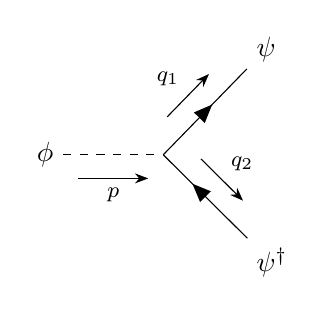
\begin{tikzpicture}
		\begin{feynman}
			\vertex (a) {\(\phi\)};
			\vertex [right=of a] (b);
			\vertex [above right=of b] (f1) {\(\psi\)};
			\vertex [below right=of b] (f2) {\(\psi^\dagger\)};
			\diagram* {
				(a) -- [scalar, momentum'={\footnotesize\(p\)}] (b),
				(b) -- [fermion, momentum={[arrow shorten=0.25]\footnotesize\(q_1\)}] (f1),
				(b) -- [anti fermion, momentum={[arrow shorten=0.25]\footnotesize\(q_2\)}] (f2),
			};
		\end{feynman}
	\end{tikzpicture}
	\hspace{2cm}
	% nucleon-anti nucleon annihilation
	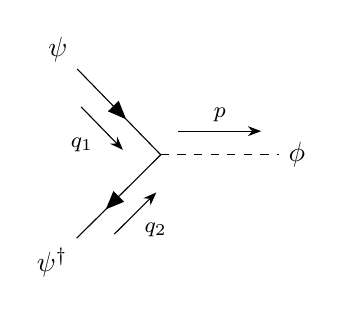
\begin{tikzpicture}
		\begin{feynman}
			\vertex (a);
			\vertex [above left=of a] (i1) {\(\psi\)};
			\vertex [right=of a] (b) {\(\phi\)};
			\vertex [below left=of a] (i2) {\(\psi^\dagger\)};
			\diagram* {
				(i1) -- [fermion, momentum'={[arrow shorten=0.25]\footnotesize\(q_1\)}] (a),
				(i2) -- [anti fermion, momentum'={[arrow shorten=0.25]\footnotesize\(q_2\)}] (a),
				(a) -- [scalar, momentum={\footnotesize\(p\)}] (b),
			};
		\end{feynman}
	\end{tikzpicture}
	\vspace{5mm}
	\caption{Feynman diagrams for meson decay (left) and nucleon-antinucleon annihilation (right).}
	\label{fig:01_qft_interactions_feynman_first_order}
\end{figure}

Explicit calculation yields the S-matrix element for both processes (Appendix~\ref{sec:01_qft_quantization_firstorder}):
\begin{equation}
	\label{eq:01_qft_interactions_yukawa_smatrix_1}
	\braket{f|S|i}^{(1)} = -ig (2\pi)^4 \delta^{(4)}(p - q_1 - q_2).
\end{equation}
The delta function ensures momentum conservation, and is in fact a general feature of all S-matrix elements.
% It also tells us that this process can only occur for $m \geq 2M$.
We typically define
\begin{equation}
	\label{eq:01_qft_interactions_matrix_element}
	\braket{f|S - \identity|i} \equiv i (2\pi)^4 \delta^{(4)}(\Sigma\,p) \mathcal M,
\end{equation}
where $\mathcal M$ is called the \textit{matrix element} of the process, and is the nontrivial component we must compute.
For our first-order processes, the matrix element is simply $\mathcal M = -g$.
However, explicit calculations quickly become intractable at higher orders; instead, we present a simpler alternative in the next section.

\subsection{Feynman diagrams}
\label{sec:01_qft_interactions_feynman}

Feynman diagrams are intuitive and powerful tools for calculating S-matrix elements. 
We have already seen examples for our first-order meson decay and nucleon-antinucleon annihilation processes in Figure~\ref{fig:01_qft_interactions_feynman_first_order}.
They encode a lot of information (some of which is redundant, shown only for these first diagrams for clarity) and, as we will see, directly give us the matrix elements of the processes.
Feynman diagrams for higher-order processes can be constructed by adding more vertices and \textit{internal lines} connecting them.
Details and some conventions used in this dissertation are given in Appendix~\ref{app:01_qft_quantization_feynman}.


\subsubsection{Feynman rules for scalar Yukawa theory}

To read off the matrix element from a Feynman diagram, we take the product of factors associated to each element of the diagram, according to the \textit{Feynman rules} of the theory.
These rules are ultimately derived from and encode all our information about the underlying Lagrangian.
They can be written in either position or momentum space; since we are working with momentum eigenstates, we will use the latter.

\begin{definition}
For our scalar Yukawa theory, the Feynman rules for calculating $i\mathcal M$ are:\footnote{These are derived nicely in Peskin and Schroeder~\cite{Peskin:1995ev} Chapter 4.7, albeit with fermionic electrons instead of our scalar ``nucleons''.}
\begin{enumerate}
	\item Vertices: \qquad
	\begin{tikzpicture}[baseline={([yshift=-0.8ex]current bounding box.center)}]
		\begin{feynman}[small]
			\vertex (a);
			\vertex [right=of a] (b);
			\vertex [above right=of b] (f1);
			\vertex [below right=of b] (f2);
			\diagram* {
				(a) -- [scalar] (b),
				(b) -- [fermion] (f1),
				(b) -- [anti fermion] (f2),
			};
		\end{feynman}
	\end{tikzpicture}
	$ = -ig$ \\[1em]
	\item Internal lines (propagators) \\[1em]
	\qquad\qquad Mesons: \quad
	\begin{tikzpicture}[baseline={([yshift=-1.8ex]current bounding box.center)}]
		\begin{feynman}[small]
			\vertex (a);
			\vertex [right=of a] (b);
			\diagram* {
				(a) -- [scalar, edge label={\footnotesize$p$}] (b) ,
			};
		\end{feynman}
	\end{tikzpicture}
	$\, = \cfrac{i}{p^2 - m^2 + i\varepsilon}$ \qquad
	Nucleons: \quad
	\begin{tikzpicture}[baseline={([yshift=-1.8ex]current bounding box.center)}]
		\begin{feynman}[small]
			\vertex (a);
			\vertex [right=of a] (b);
			\diagram* {
				(a) -- [fermion, edge label={\footnotesize$q$}] (b),
			};
		\end{feynman}
	\end{tikzpicture}
	$\, = \cfrac{i}{q^2 - M^2 + i\varepsilon}$ \\[1em]
	\item Impose momentum conservation at each vertex.
	\item Integrate over the momentum $k$ flowing through each loop $\int \cnicefrac{d^4k}{(2\pi)^4}$.
\end{enumerate}

\end{definition}
Note that the factors associated with internal lines are exactly the Feynman propagators from Section~\ref{sec:01_qft_quantization_propagators}, which is in line with their interpretation as the amplitude for a particle to propagate from one point to another.
For internal lines, the convention is for momentum to flow in the same direction as the particle flow, even for antiparticles.
We see immediately that these rules reproduce the matrix element $\mathcal M = -g$ for our first-order processes, as expected.
We discuss loops briefly at the end of this section; however, we focus primarily on \textit{tree-level diagrams}, those without loops.
% We next look at some more complicated, higher order diagrams.

\subsubsection{Nucleon-antinucleon scattering}

One interesting higher-order example is nucleon-antinucleon scattering $\psi\psi^\dagger \rightarrow \psi\psi^\dagger$.
At lowest order, we have the diagrams shown in Figure~\ref{fig:01_qft_interactions_feynman_na_scattering}.
% Now, these are two distinct particles, so we do not have the $u$-channel diagram with the final states interchanged as above.
% %  (it is also not allowed for the Yukawa interaction).
% However, we do have a new $s$-channel diagram on the right.

\begin{figure}[ht]
	\centering
	\captionsetup{justification=centering}
	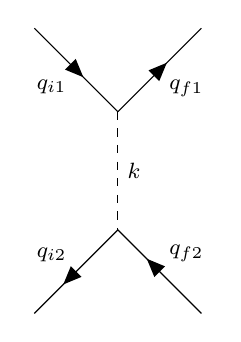
\begin{tikzpicture}
		\begin{feynman}
			\vertex (a);
			\vertex [below=of a] (b);
			\vertex [above left=of a] (i1);
			\vertex [below left=of b] (i2);
			\vertex [above right=of a] (f1);
			\vertex [below right=of b] (f2);
			\diagram* {
				(a) -- [scalar, edge label={\footnotesize\(k\)}] (b),
				(i1) -- [fermion, edge label'={\footnotesize\(q_{i1}\)}] (a),
				(i2) -- [anti fermion, edge label={\footnotesize\(q_{i2}\)}] (b),
				(a) -- [fermion, edge label'={\footnotesize\(q_{f1}\)}] (f1),
				(b) -- [anti fermion, edge label={\footnotesize\(q_{f2}\)}] (f2),
			};
		\end{feynman}
	\end{tikzpicture}
	\hspace{3cm}
	% s-channel
	\raisebox{7mm}{
	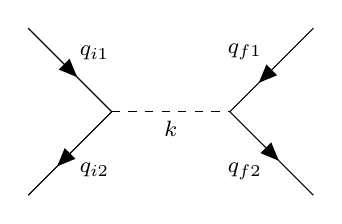
\begin{tikzpicture}
		\begin{feynman}
			\vertex (a);
			\vertex [right=of a] (b);
			\vertex [above left=of a] (i1);
			\vertex [below left=of a] (i2);
			\vertex [above right=of b] (f1);
			\vertex [below right=of b] (f2);
			\diagram* {
				(a) -- [scalar, edge label'={\footnotesize\(k\)}] (b),
				(i1) -- [fermion, edge label={\footnotesize\(q_{i1}\)}] (a),
				(i2) -- [anti fermion, edge label'={\footnotesize\(q_{i2}\)}] (a),
				(b) -- [anti fermion, edge label={\footnotesize\(q_{f1}\)}] (f1),
				(b) -- [fermion, edge label'={\footnotesize\(q_{f2}\)}] (f2),
			};
		\end{feynman}
	\end{tikzpicture}
	}
	\vspace{5mm}
	\caption{The two lowest order nucleon-antinucleon scattering diagrams.}
	\label{fig:01_qft_interactions_feynman_na_scattering}
\end{figure}

The first two Feynman rules result in the same matrix element (Eq.~\ref{eq:01_qft_interactions_nn_scattering_1}) for both.
Imposing momentum conservation we find:
\begin{equation}
	\label{eq:01_qft_interactions_na_scattering}
	\begin{split}
		i \mathcal M = i(\mathcal M_{\mathrm{left}} + \mathcal M_{\mathrm{right}}) &= (-ig)^2 \bigg[ \cfrac{1}{(q_{f1} - q_{i1})^2 - m^2} + \cfrac{1}{(q_{i1} + q_{i2})^2 - m^2} \bigg]. 
		% \\
		% &= (-ig)^2 \bigg( \cfrac{1}{t - m^2} + \cfrac{1}{s - m^2} \bigg)
	\end{split}
\end{equation}



\subsubsection{Virtual particles}

Note that by momentum conservation, the exchange meson does not have mass $m$, as $k^2 \neq m^2$.
We say that this meson is a \textit{virtual particle} and is \textit{off-shell} (referring to the ``mass shell'' in $k$ at $k^2 = m^2$).
This may appear dangerously unphysical; however, we are saved by the fact that such off-shell particles always appear internally in the diagram and thus can never be observed.
% Their physical interpretation is quite unclear; 
In a sense, they can be viewed simply as a mathematical convenience in QFT; no one knows their correct physical interpretation, if any.\footnote{To quote Hong Liu, ``In physics, when we don't understand something, we give it a name and then claim we understand it.''~\cite{LiuRQFT}.}


\subsubsection{Mandelstam variables}

Because these types of 2-by-2 scattering processes are so common in particle physics, they have standard names, based on the momenta in the denominator of the matrix element.

\begin{definition}
	For incoming particle momenta $p_{i1}$ and $p_{i2}$ and outgoing momenta $p_{f1}$ and $p_{f2}$, the \textit{Mandelstam variables} are defined as:
	\begin{equation}
		\label{eq:01_qft_interactions_mandelstam}
		\begin{split}
			s &= (p_{i1} + p_{i2})^2 = (p_{f1} + p_{f2})^2, \\
			t &= (p_{i1} - p_{f1})^2 = (p_{i2} - p_{f2})^2, \\
			u &= (p_{i1} - p_{f2})^2 = (p_{i2} - p_{f1})^2.
		\end{split}
	\end{equation}
\end{definition}

We can see that the matrix elements for nucleon-antinucelon scattering (Eq.~\ref{eq:01_qft_interactions_na_scattering}) can be rewritten in terms of $t$ and $s$ as:
\begin{equation}
	\label{eq:01_qft_interactions_nn_tchannel_uchannel}
	\begin{split}
		i \mathcal M_{\mathrm{left}} = (-ig)^2 \cdot \cfrac{1}{t - m^2}, \\
		i \mathcal M_{\mathrm{right}} = (-ig)^2 \cdot \cfrac{1}{s - m^2}.
	\end{split}
\end{equation}
Hence, they are referred to as $t$-channel and $s$-channel diagrams, respectively.
An example of a $u$-channel diagram appears for nucleon-nucleon scattering in Figure~\ref{fig:01_qft_interactions_feynman_nn_scattering}.
% We will see an example of an $s$-channel diagram in the next example.
Intuitively, $s$ is the total energy in the COM frame squared, while $t$ and $u$ are a measure of how much momentum is exchanged between the scattered particles (see Appendix~\ref{app:01_qft_quantization_feynman}).


\subsubsection{Resonances}

Note an important point about $s-$channel diagrams: the amplitude diverges as $s \rightarrow m^2$.\footnote{We are saved from this potential infinity by a factor to be added to the denominator due to meson decay (Tong SM~\cite{TongSM} Chapter 3.5).}
Or, in other words, as the COM energy approaches the mass of the exchanged particle (as long as $m > 2M$).

This divergence is interpreted as a \textit{resonance} in the cross section (see below) of the scattering process as a function of $\sqrt{s}$, and allows us to discover new particles.
Figure~\ref{fig:01_qft_interactions_eezpeak} shows a great example for $e^+e^- \rightarrow$ hadron scattering by a series of HEP experiments with a magnificent peak at 96\GeV, the $Z$ boson mass.

\begin{figure}
	\centering
	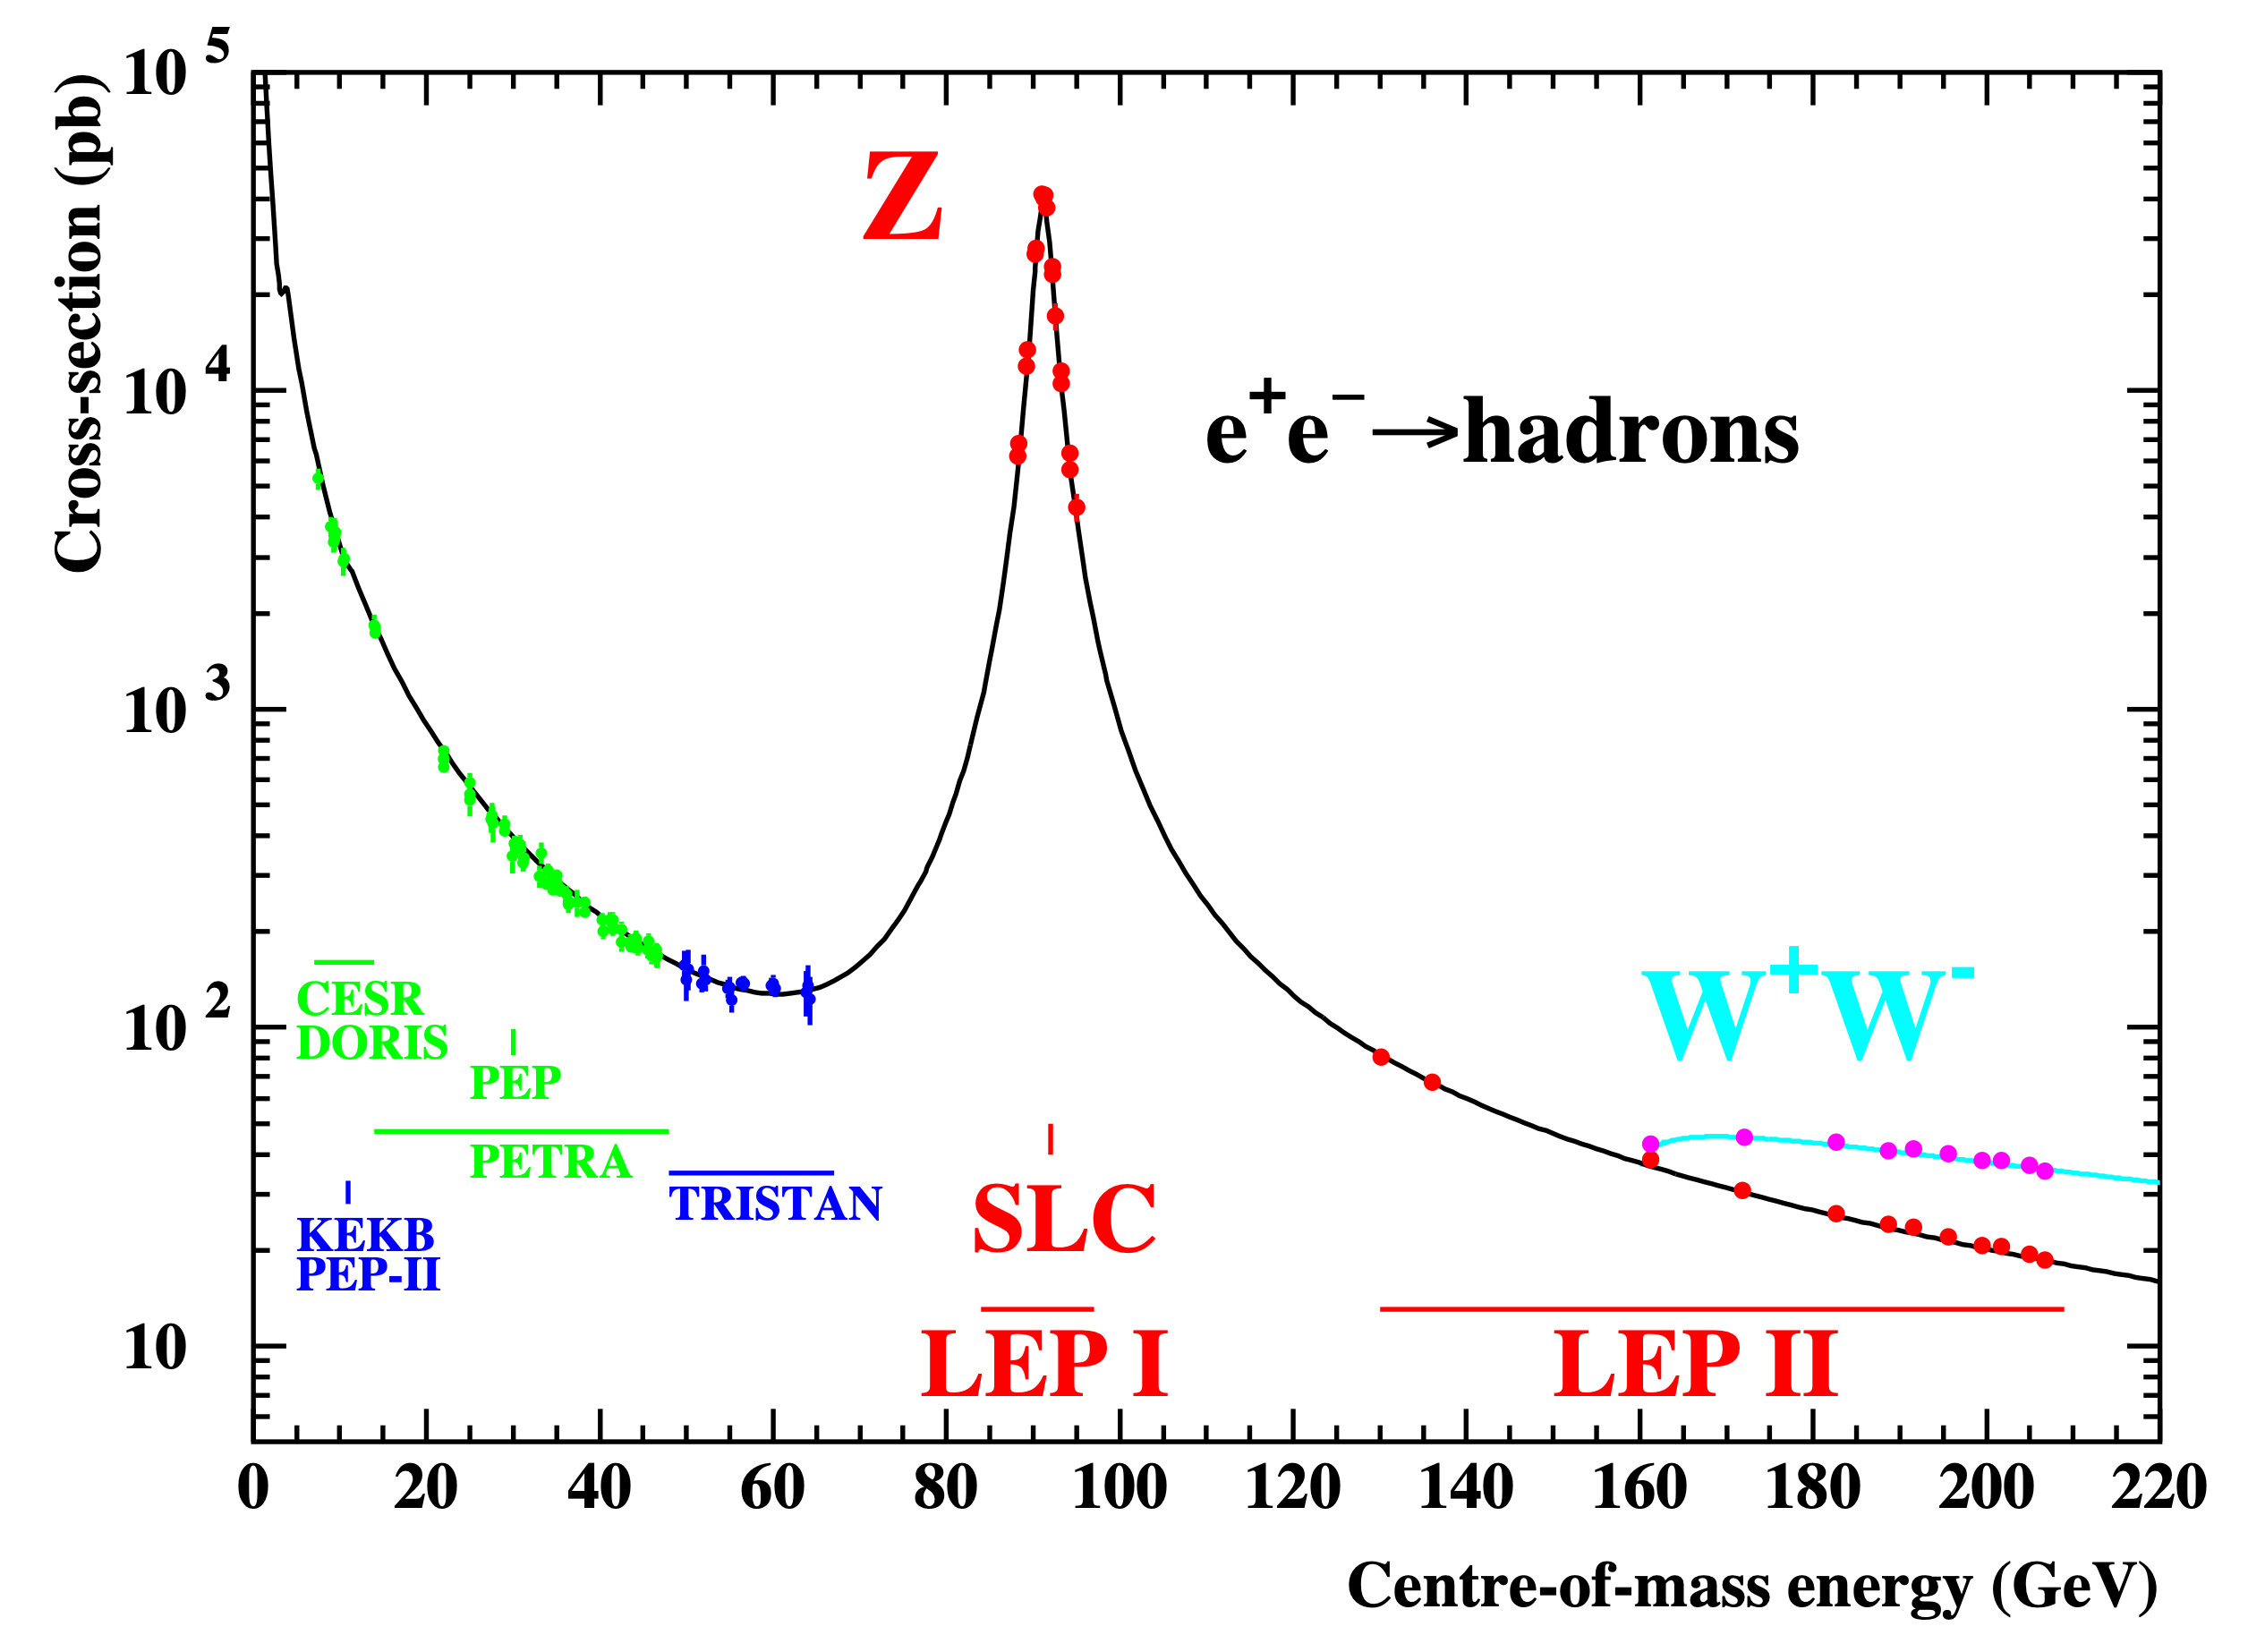
\includegraphics[width=0.8\textwidth]{figures/01-SM-02-QFT/eezpeak}
	\caption{Cross section for $e^+e^- \rightarrow$ hadron scattering as a function of $\sqrt{s}$ with a clear resonance at the $Z$ boson mass, reproduced from Ref.~\cite{ALEPH:2005ab}.}
	\label{fig:01_qft_interactions_eezpeak}
\end{figure}


\subsubsection{The classical limit and the Yukawa potential}

It is important to check our QFT recovers classical physics in the appropriate limit.
It will also be useful to translate the somewhat abstract idea of amplitudes to the familiar concepts of forces and potentials.
We will do so by considering the nonrelativistic limit ($\abs{\cvec{p}} \ll M$) of our above amplitudes and using the Born approximation relating the scattering amplitude between two particles to the potential between them $U(\cvec{r})$:
\begin{equation}
	\label{eq:01_qft_interactions_born}
	\mathcal M = \braket{\cvec{p}_f|U(\cvec{r})|\cvec{p}_i} = -i \int U(\cvec{r}) e^{i(\cvec{p}_f - \cvec{p}_i)\cdot\cvec{r}} d^3r,
\end{equation}
where $\cvec{r}$ is the displacement between the particles.

First, let us consider what this potential would be classically.
The static Klein-Gordon equation for a delta-function source:
\begin{equation}
	\label{eq:01_qft_interactions_static_kg}
	(\nabla^2 - m^2) \phi(\cvec{r}) = \delta^3(\cvec{r}),
\end{equation}
can be found via the Fourier transform to be:
\begin{equation}
	\label{eq:01_qft_interactions_static_kg_solution}
	\phi(\cvec{r}) =  \cfrac{e^{-mr}}{4\pi r}.
\end{equation}
We can interpret this to be the profile of $\phi$ around a nucleon (the delta function source), and thus conversely the potential felt by another nucleon via the meson and the Yukawa interaction, under the assumption $M \gg m$.
This is entirely analogous to gauge potential $A_0$ in electrostatics generated by a $\delta$-function source acting as the electric potential for a test charge.

Going back to our amplitude for nucleon-antinucleon scattering, the $s$-channel diagram vanishes in the nonrelativistic limit (which essentially means it does not have a simple classical interpretation), while the $t$-channel diagram actually stays the same:
\begin{equation}
	\label{eq:01_qft_interactions_na_scattering_nr}
	i \mathcal M = -(-ig)^2 \cdot \cfrac{1}{\abs{\cvec{p}_f - \cvec{p}_i}^2 - m^2}.
\end{equation}
Plugging this into the LHS of Eq.~\ref{eq:01_qft_interactions_born} and inverting the RHS integral gives us:
\begin{equation}
	\label{eq:01_qft_interactions_yukawa_potential}
	U(\cvec{r}) = -\cfrac{g^2}{4M^2} \cdot \cfrac{e^{-mr}}{4\pi r}.
\end{equation}
This is exactly the classical potential we found in Eq.~\ref{eq:01_qft_interactions_static_kg_solution}!
It is weighted by the coupling constant $g$ and $M$ to get the correct dimensions, and with a minus sign telling us potential is attractive.

Thus, we are able to reproduce Newtonian forces from the nonrelativisic limit of QFT.
We also have the new interpretation of forces as simply manifestations of interactions in the Lagrangian, occurring through the exchange of virtual particles.

This potential is called the \textit{Yukawa potential}, describing a force mediated by a massive boson.
As expected, in the limit $m \rightarrow 0$, we recover the familiar $1/r$ Coulomb potential, which is mediated by the massless photon.
We can check that we obtain the same potential for nucleon-nucleon scattering and, more generally, that all forces mediated by scalars are attractive.
In fact, this is true for spin-2 particles as well, which is why gravity is universally attractive!
On the other hand, forces mediated by spin-1 particles, such as EM, can be either attractive or repulsive, with the charges of the particles involved determining the sign of each diagram.
See e.g. Zee QFT~\cite{Zee:2003mt} Chapter I.5 for a useful discussion.


\subsubsection{Fourth-order diagrams and loops}

So far, we have only considered \textit{tree-level} diagrams, the simplest to calculate.
This is in contrast to diagrams with \textit{loops}, which can occur at higher order in perturbation theory.
For example, at fourth-order we can have diagrams like those in Figure~\ref{fig:01_qft_interactions_feynman_loops} for nucleon scattering. 

Such diagrams contribute integrals over the loop momentum $k$ to the matrix element, which can notoriously diverge.
To deal with this requires a process called \textit{renormalization}, which, briefly, involves defining a cut-off energy scale $\Lambda$ for these integrals, beyond which we claim the theory is invalid.
Experimentally, the main consequence is that physical parameters like the mass of particles and coupling constants in fact depend on the energy scale at which they are measured!

\begin{figure}[ht]
	\centering
	\captionsetup{justification=centering}
	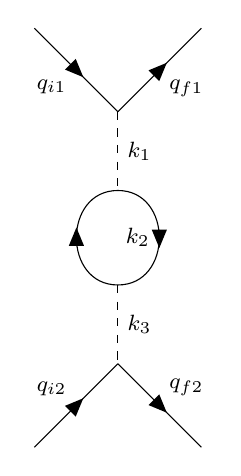
\begin{tikzpicture}
		\begin{feynman}
			\vertex (a);
			\vertex [below=1cm of a] (c);
			\vertex [below=1.2cm of c] (d);
			\vertex [below=1cm of d] (b);
			\vertex [above left=of a] (i1);
			\vertex [below left=of b] (i2);
			\vertex [above right=of a] (f1);
			\vertex [below right=of b] (f2);
			\diagram* {
				(a) -- [scalar, edge label={\footnotesize$k_1$}] (c),
				(d) -- [scalar, edge label={\footnotesize$k_3$}] (b),
				(i1) -- [fermion, edge label'={\footnotesize$q_{i1}$}] (a),
				(i2) -- [fermion, edge label={\footnotesize$q_{i2}$}] (b),
				(a) -- [fermion, edge label'={\footnotesize$q_{f1}$}] (f1),
				(b) -- [fermion, edge label={\footnotesize$q_{f2}$}] (f2),
				(c) -- [fermion, half left, edge label'={\footnotesize$k_2$}] (d),
				(d) -- [fermion, half left] (c),
			};
		\end{feynman}
	\end{tikzpicture}
	\caption{An example of a higher-order scattering diagram with a ``loop''.}
	\label{fig:01_qft_interactions_feynman_loops}
\end{figure}

\subsection{Decay rates and cross sections}
\label{sec:01_qft_interactions_decay}

In this section, we translate our S-matrix elements to physical observables: cross sections and decay rates.

\subsubsection{Cross section}

Classically for a scattering experiment, the number of particles scattered $N$ is related to the cross sectional area $\sigma$ as:
\begin{equation}
	\label{eq:01_qft_interactions_cross_section_classical}
	N = \sigma T \Phi,
\end{equation}
where $T$ is the total time and $\Phi$ is the flux of incoming particles (number of incoming particles per unit area and unit time).
In QM, we define the cross section $\sigma$ similarly, but in terms of the probability of scattering $P$ instead of $N$:
\begin{equation}
	\label{eq:01_qft_interactions_cross_section_qm}
	\sigma = \frac{P}{\Phi T}.
\end{equation}
This is a more abstract quantity in QM, but it still has units of area.
The number of scattering events $N$ is related to $\sigma$ by a factor we call the \textit{luminosity} $L$:
\begin{equation}
	\label{eq:01_qft_interactions_cross_section_luminosity}
	N = \sigma L.
\end{equation}
Here, we simply consider this the definition of luminosity, but for a collider, for example, it can be derived from the properties of the input particle beams  (as will be discussed in Part~\ref{part:epp}).
Often, we are interested in the \textit{differential cross section} $d\sigma$ with respect to kinematic variables like the solid angle $\Omega$ or energy, so we write:
\begin{equation}
	\label{eq:01_qft_interactions_cross_section_differential}
	d\sigma = \frac{dP}{\Phi T}.
\end{equation}

As in QM, this probability $P$ is proportional to the square of the amplitude $|\braket{f|S|i}|^2$:
\begin{equation}
	\label{eq:01_qft_interactions_cross_section_probability}
	dP = \frac{\abs{\braket{f|S|i}}^2}{\braket{f|f}\braket{i|i}}\, d\Pi,
\end{equation}
where $\braket{f|f}$ and $\braket{i|i}$ are the normalization factors for the final and initial states (they are not equal to $1$ as discussed in Section~\ref{sec:01_qft_quantization_propagators}), and $d\Pi$ is the differential region of final state momenta.

For the case of two incoming particles (which is what is most relevant for this dissertation), we can put all of this together to obtain the relation between differential cross section and the matrix element $\mathcal M$:
\begin{equation}
	\label{eq:01_qft_interactions_cross_section_matrix_element}
	d\sigma = \frac{1}{(2E_1)(2E_2)\abs{\cvec{v}_1 - \cvec{v}_2}} \abs{\mathcal M}^2 d\Pi_{\mathrm{LIPS}},
\end{equation}
where $E_1$ and $E_2$ are the energies of the incoming particles, $\cvec{v}_1$ and $\cvec{v}_2$ are their velocities, and $d\Pi_{\mathrm{LIPS}}$ is called the Lorentz-invariant phase space of the final state momenta:
\begin{equation}
	\label{eq:01_qft_interactions_cross_section_lips}
	d\Pi_{\mathrm{LIPS}} = (2\pi)^4 \delta^{(4)}(\Sigma p) \prod_{\mathrm{final\ states}\ j} \frac{d^3p_j}{(2\pi)^3} \frac{1}{2E_j}
\end{equation}

For the case of $2 \rightarrow 2$ scattering, in the COM frame, this simplifies considerably:
\begin{equation}
	\label{eq:01_qft_interactions_cross_section_com}
	\bigg(\frac{d\sigma}{d\Omega}\bigg)_{\mathrm{CM}} = \frac{1}{64\pi^2E_{\mathrm{CM}}^2}\, \frac{\abs{\cvec{p}_f}}{\abs{\cvec{p}_i}} \abs{\mathcal M}^2 \theta(E_{\mathrm{CM}} - m_3 - m_4),
\end{equation}
and even more so when the all four masses are equal:
\begin{equation}
	\label{eq:01_qft_interactions_cross_section_com_equal_mass}
	\bigg(\frac{d\sigma}{d\Omega}\bigg)_{\mathrm{CM}} = \frac{1}{64\pi^2E_{\mathrm{CM}}^2}\, \abs{\mathcal M}^2.
\end{equation}

% For nucleon-nucleon scattering in the COM frame, for example, we have (at tree level):
% \begin{equation}
% 	\label{eq:01_qft_interactions_nn_scattering_cross_section}
% 	\begin{split}
% 		\bigg(\frac{d\sigma(\theta)}{d\Omega}\bigg)_{\mathrm{CM}} &= \frac{g^4}{64\pi (2E)^2} \left(\frac{1}{t - m^2} + \frac{1}{u - m^2}\right)^2 \\
% 		&= \frac{g^4}{64\pi (2E)^2} \left[\frac{1}{2p^2(1 - \cos\theta) - m^2} + \frac{1}{2p^2(1 + \cos\theta) - m^2}\right]^2,
% 	\end{split}
% \end{equation}
% where we used the expressions for $t$ and $u$ for a collision along the z-axis from Eq.~\ref{eq:01_qft_interactions_mandelstam_com}.

\subsubsection{Decay rate}

The other type of process we are interested in are decays.
The decay rate $\Gamma$ is simply the probability of decay per unit time:
\begin{equation}
	\label{eq:01_qft_interactions_decay_rate}
	\Gamma =  \frac{P}{T}.
\end{equation}
Using our expression for $P$ from above and simplifying, we find:
\begin{equation}
	\label{eq:01_qft_interactions_differential_decay_rate}
	d\Gamma = \frac{1}{2m} \abs{\mathcal M}^2 d\Pi_{\mathrm{LIPS}},
\end{equation}
in the rest frame of the decaying particle, where $m$ is its mass.
If multiple decays of the same particle are possible, we sum over the final states in the phase space integral.
The total $\Gamma$ is then called the \textit{width} of the particle, and $1/\Gamma \equiv \tau$ is its half-life.

For our simple meson decay $\phi \rightarrow \psi^\dagger\psi$, we have at tree level:
\begin{equation}
	\label{eq:01_qft_interactions_decay_rate_meson_decay}
	d\Gamma = \frac{g^2}{2m} d\Pi_{\mathrm{LIPS}} \quad \Rightarrow \quad \Gamma = \frac{g^2}{32\pi m} \left(1 - \frac{4M^2}{m^2}\right)^{1/2},
\end{equation}
where we performed the integral over $d\Pi_{\mathrm{LIPS}}$ (see Ref.~\cite{XianyuPSSolutions} 4.2).
This is in fact not too far off the expression for the decay width of the Higgs boson to fermions.
What we are missing of course is that fermions are spin-$\cnicefrac{1}{2}$ particles, and we need to sum over their spin states.
Fermions are described by spinor field theory, detailed in Appendix~\ref{sec:01_qft_spinors}.

\section{Gauge theories}
\label{sec:01_qft_gt}

% \begin{center}
% 	\centering
{
	\noindent
	\textit{Nature seems to take advantage of the simple mathematical representations of the symmetry laws. 
	When one pauses to consider the elegance and the beautiful perfection of the mathematical reasoning involved and contrast it with the complex and far-reaching physical consequences, a deep sense of respect for the power of the symmetry laws never fails to develop.} --- C. N. Yang
}
% \end{center}

\

So far, we have discussed spin-$0$ scalar bosons (and the spin-$\frac{1}{2}$ fermions in Appendix~\ref{sec:01_qft_spinors}); the last set of SM particles are the spin-$1$ \textit{gauge bosons}.
These are the particles which mediate all three fundamental forces in the SM: electromagnetism, the weak force, and the strong force.
Fortunately, compared to spinors, they live in the simpler and familiar vector representation of the Lorentz group.

On the other hand, they are intrinsically tied to a unique type of internal, \textit{local}, symmetry in QFT: \textit{gauge symmetry}.
Unlike, say, Lorentz or spacetime translation invariance, this is not a fundamental physical symmetry of nature, and is not associated with any consrervation law.
Instead, it simply describes a redundancy in our mathematical formulation of the gauge theory, stemming from the fact that the vector fields used to describe the gauge bosons have more degrees of freedom (DoFs) than the physical particles themselves.
The DoFs are thereby reduced by identifying fields related by a gauge symmetry transformation to be the same physical state, known as the principle of \textit{gauge invariance}.
This is entirely analogous to requiring that a change of coordinate system not affect the physics.
A deeper discussion of the motivations behind gauge invariance can be found in Appendix~\ref{sec:01_qft_gt_why}.
% In this section, we first discuss the motivations for gauge invariance in QFT in Section~\ref{sec:01_qft_gt_why}.

In this section, we first introduce the simplest gauge boson, the photon, and its associated \UU[1] gauge symmetry in Section~\ref{sec:01_qft_gt_maxwell}.
Coupling this to matter and quantizing the theory gives us QED, the relativistic quantum theory of electromagnetism (Section~\ref{sec:01_qft_gt_qed}).
We then generalize this to, and quantize, non-abelian gauge theories, known as Yang-Mills theories, in Sections~\ref{sec:01_qft_gt_yangmills} and~\ref{sec:01_qft_gt_ymquant}, respectively.
We conclude with a discussion of renormalization and the \textit{running} of coupling constants in Section~\ref{sec:01_qft_gt_asymptotic}.


\subsection{Maxwell Theory}
\label{sec:01_qft_gt_maxwell}

Gauge symmetries are a generalization of internal global symmetries, such as the \UU[1] symmetry from Section~\ref{sec:01_qft_classical_symmetries}, to a \textit{local} symmetry, where the symmetry transformation can be a function of spacetime.
We are most familiar with this concept from classical E\&M, in which Maxwell's laws are invariant under transformations of the $4$-vector potential $A_\mu = (\phi, \cvec{A})$ of the form:
\begin{equation}
	\label{eq:01_qft_gt_maxwell_gauge}
	A_\mu(x) \rightarrow A_\mu(x) + \frac{1}{e}\partial_\mu\alpha(x),
\end{equation}
for an arbitrary function $\alpha(x)$, where $e$ is a conventional constant that we will soon interpret as the coupling constant of the theory.
% Remarkably, once quantized, $A_\mu$ represents the photon field.

Recall that $A_\mu$ is related to the electric and magnetic fields, $\cvec{E}$ and $\cvec{B}$, by:
\begin{equation}
	\label{eq:01_qft_gt_maxwell_fields}
	\cvec{E} = -\nabla\phi - \partial_t\cvec{A}, \qquad \cvec{B} = \nabla\times\cvec{A},
\end{equation}
and the Maxwell equations can be derived from the Lagrangian:
\begin{equation}
	\label{eq:01_qft_gt_maxwell_lagrangian}
	\mathcal L = -\frac{1}{4}F_{\mu\nu}F^{\mu\nu},
\end{equation}
where
\begin{equation}
	\label{eq:01_qft_gt_maxwell_field_strength}
	F_{\mu\nu} = \partial_\mu A_\nu - \partial_\nu A_\mu
\end{equation}
is the \textit{field strength} tensor.
One can confirm that (1) $F_{\mu\nu}$ and, hence, the Lagrangian is invariant under the gauge transformation in Eq.~\ref{eq:01_qft_gt_maxwell_gauge}, and (2) the resulting E-L EOMs are exactly the homogeneous Maxwell equations.
Thus, classical E\&M was our earliest and simplest gauge theory, although the significance and generalization of gauge invariance only became clear with the advent of QFT.

Gauge invariance significantly restricts the possible terms in the Lagrangian (and thus considerably simplifies the theory).
Notably, mass terms like $m^2A_\mu^2$ \textit{violate} gauge invariance, which is why gauge bosons are necessarily massless, without something special like the Higgs mechanism (Section~\ref{sec:01_qft_higgs}).
As discussed in Appendix~\ref{sec:01_qft_gt_why}, gauge invariance also ensures the renormalizability of the theory and reduces the DoFs of $A_\mu$ such that, once quantized, we can identify it as the photonic field.

% Finally, note that our Lagrangian contains terms of the form $(\partial_\mu A_\nu)^2$; hence, $A_\mu$ (and all spin-$1$ fields) have dimension $1$.

\subsubsection{Interactions with scalars}

The \UU[1] nature of the gauge transformation becomes more apparent when we try to couple the photon to other particles.
Note that our Lagrangian above contains terms of the form $(\partial_\mu A_\nu)^2$ so $A_\mu$ (and indeed all spin-$1$ fields) have dimension $1$.

% \subparagraph{Coupling to scalars}
Let us consider a scalar field $\phi$: we can write renormalizable, scalar terms like $A_\mu^2\phi^2$ and $A_\mu \phi\partial_\mu\phi$; however, they do not look gauge invariant.
To make them so, we must require that $\phi$ \textit{also} transforms under the same gauge transformation in a way that compensates the change in $A_\mu$.

The simplest way is to take $\phi$ to be a \textit{complex} scalar field and ``promote'' its inherent global \UU[1] symmetry to a local one:
\begin{equation}
	\label{eq:01_qft_gt_maxwell_scalar_gauge}
	\phi(x) \rightarrow e^{iQ_\phi\alpha(x)}\phi(x),
\end{equation}
where we say $Q_\phi$ represents the charge of $\phi$ under the \UU[1] symmetry.\footnote{Note that such a transformation is not possible with a \textit{real} field, which necessarily has $0$ charge and does not couple with the photon.}
% Since we will not be discussing more than one interacting field until the next chapter, we will henceforth take $Q = 1$ for simplicity.
We can then define the \textit{covariant derivative} acting on $\phi$ as:\footnote{As discussed above, this is the same concept as the covariant derivative in GR, with the gauge field $A_\mu$ acting as a connection on a \UU[1] fiber bundle analogously to the Levi-Civita connection between tangent bundles.
Essentially, it encodes the change in the local phase of $\phi$ across spacetime (see Peskin and Shroeder~\cite{Peskin:1995ev} Chapter 15.1 for a nice derivation of this).
}
\begin{equation}
	\label{eq:01_qft_gt_maxwell_covariant_derivative}
	D_\mu\phi = (\partial_\mu - ieQ_\phi A_\mu)\phi,
\end{equation}
where $e$ is the same coupling constant from Eq.~\ref{eq:01_qft_gt_maxwell_gauge}.

One can check that $D_\mu\phi$ transforms under the gauge transformation as:
\begin{equation}
	\label{eq:01_qft_gt_maxwell_covariant_derivative_gauge}
	D_\mu\phi \rightarrow e^{iQ_\phi\alpha(x)}D_\mu\phi,
\end{equation}
meaning $(D_\mu\phi)^\dagger D^\mu\phi$ provides us with a gauge invariant interaction term for the Lagrangian.
Thus, we have a gauge invariant \textit{scalar} QED Lagrangian:
\begin{equation}
	\label{eq:01_qft_gt_maxwell_scalar_lagrangian}
	\mathcal L = -\frac{1}{4}F_{\mu\nu}F^{\mu\nu} + (D_\mu\phi)^\dagger D^\mu\phi - m^2\abs{\phi}^2.
\end{equation}

Note that the commutator of the covariant derivative is in fact not a derivative at all, but proportional to the field strength tensor:
\begin{equation}
	[D_\mu, D_\nu]\phi = ([\partial_\mu, \partial_\nu] - ie[\partial_\mu, A_\nu] + ie[\partial_\nu, A_\mu])\phi = -ieF_{\mu\nu}\phi.
\end{equation}
Thus, we can define $F_{\mu\nu} \equiv \frac{i}{e}[D_\mu, D_\nu]$, which will prove useful for non-abelian gauge symmetries later in this section.
% By definition, higher order covariant derivatives transform the same way as the first order, meaning $F_{\mu\nu}$ transforms as $F_{\mu\nu} \rightarrow 

Generally, we choose the normalization $Q_e = -1$ for the electron field, so $e$ becomes our familiar elementary charge (in natural units) and $\alpha\equiv\cnicefrac{e^2}{4\pi} \approx \cnicefrac{1}{137}$ is the famous dimensionless fine structure constant.\footnote{Technically, this value varies with our energy scale, as we will discuss in Section~\ref{sec:01_qft_gt_asymptotic}, and $\cnicefrac{1}{137}$ is its asymptotic value at low energies.}

\subsubsection{Interactions with spinors}

The case for spinors is not so different. 
The definition of the covariant derivative remains the same, so combining the ``covariant'' Dirac Lagrangian with the free photonic yields the QED Lagrangian:
\begin{equation}
	\label{eq:01_qft_gt_maxwell_qed_lagrangian}
	\mathcal L = -\frac{1}{4}F_{\mu\nu}F^{\mu\nu} + \bar\psi(i\cslashed D - m)\psi.
\end{equation}
This is in fact the most general possible Lorentz-invariant, renormalizable, $P$-symmetric Lagrangian for a spinor field with a \UU[1] gauge symmetry, and can thus be derived from the requirement of gauge invariance alone (as done in e.g. Peskin and Shroeder~\cite{Peskin:1995ev} Chapter 15.1).
This is a general feature of the SM: every possible term permitted by gauge invariance and the usual physical requirements of Lorentz invariance etc. is included in the Lagrangian (with one possible exception that forms the basis for the strong CP problem~\cite{Wu:1991rw,Mannel:2007zz}).

Expanding out the Lagrangian, we have:
\begin{equation}
	\label{eq:01_qft_gt_maxwell_qed_lagrangian_expanded}
	\mathcal L = -\frac{1}{4}F_{\mu\nu}F^{\mu\nu} + \bar\psi(i\gamma^\mu\partial_\mu - m)\psi - e\bar\psi\gamma^\mu\psi A_\mu,
\end{equation}
where we see this interaction term is simply $-ej^\mu A_\mu$ with $j^\mu = \bar\psi\gamma^\mu\psi$ the conserved current associated with the \textit{global} \UU[1] symmetry we found in Section~\ref{sec:01_qft_spinors_lagrangian}.
One can check that the E-L EOMs for $A_\mu$ now correspond to the \textit{inhomogeneous} Maxwell equations with a source term $J_\mu \equiv -ej_\mu$:
\begin{equation}
	\label{eq:01_qft_gt_maxwell_qed_inhomo_eqs}
	\partial_\mu F_{\mu\nu} = J_\nu,
\end{equation}
reproducing our beloved E\&M from this field theory formulation!
% \TODO{We will discuss Feynman diagrams and important processes in the next chapter?}

\subsection{Quantum electrodynamics}
\label{sec:01_qft_gt_qed}

The quantized version of the above is what we call \textit{quantum electrodynamics} (QED): the QFT of electromagnetic interactions.
It has proven an extraordinarily successful theory, serving as a model for the remainder of the SM as well as theories for condensed matter phenomena.

The exact path to quantizing $A_\mu$ depends on the choice of gauge.
We will forego those details and simply use physical intuition --- namely, that the photon has only two physical, transverse polarizations --- to motivate the result:
\begin{equation}
	\label{eq:01_qft_gt_maxwell_quantization}
	A_\mu(x) = \int \frac{d^3p}{(2\pi)^3} \frac{1}{\sqrt{2E_p}} \sum_{\lambda=1}^2 \left(\epsilon_\mu^\lambda(p)\hat a^\lambda_p e^{-ip\cdot x} + \epsilon_\mu^{\lambda*}(p) \hat a^{\lambda\dagger}_p e^{ip\cdot x}\right),
\end{equation}
where $\epsilon_\mu^\lambda(p)$ are the two transverse polarization basis vectors and $a_p^\lambda$ and $a^{\lambda\dagger}_p$ are the photon annihilation and creation operators.

The photon propagator depends as well on the choice of gauge.
Expanding the homogeneous photon EOM, Eq.~\ref{eq:01_qft_gt_maxwell_qed_inhomo_eqs}, gives:
\begin{equation}
	\label{eq:01_qft_gt_maxwell_photon_eom_psapce}
	\partial_\mu\partial^\mu A_\nu - \partial_\nu\partial_\mu A^\mu = J_\nu,
\end{equation}
which in momentum space becomes:
\begin{equation}
	\label{eq:01_qft_gt_maxwell_photon_eom_momentum}
	(-p^2 \eta_{\mu\nu} + p_\mu p_\nu) A_\mu  = J_\nu.
\end{equation}
Recall that the propagator is the inverse of the operator on the LHS for a delta-function source; however, due to the redundant DoFs of $A_\mu$, this is not directly invertible without first fixing a gauge.

The cleanest way to do so is to add a ``Lagrange multiplier'' term representing the gauge fixing condition to the Lagrangian.
The most common choice is the \textit{Lorenz gauge}, $\partial_\mu A^\mu = 0$, which makes Lorentz-invariance manifest and to enforce which we can include the term $-\frac{1}{2\xi}(\partial_\mu A^\mu)^2$.
One can confirm that the EOM for $\xi$ is exactly the Lorenz gauge condition.
Inverting the new EOM for $A_\mu$ gives us the (Feynman) photon propagator:
\begin{equation}
	\label{eq:01_qft_gt_maxwell_photon_propagator}
	\Delta_{\mu\nu}(p) = \frac{-i}{p^2 + i\epsilon}\left[ \eta_{\mu\nu} + (1-\xi)\frac{p_\mu p_\nu}{p^2} \right].
\end{equation}
This is called the $R_\xi$ gauge and different values of $\xi$ correspond to different propagators, each with their own advantages and disadvantages for calculations.
In QED, we typically take $\xi = 1$, called the Feynman-'t Hooft gauge, for simplicity:
\begin{equation}
	\label{eq:01_qft_gt_maxwell_photon_propagator_feynman}
	\Delta_{\mu\nu}(p) = \frac{-i \eta_{\mu\nu}}{p^2 + i\epsilon}.
\end{equation}

\begin{definition}
	\label{def:01_qft_gt_maxwell_feynman}
	With this, we can write down the Feynman rules for QED, with spinor ($\alpha$, $\beta$) and $4$-vector ($\mu$, $\nu$) indices labeled explicitly for clarity:
	% % feynman rules for QED
\begin{enumerate}
	\item Vertices: \qquad
	\begin{tikzpicture}[baseline={(current bounding box.center)}]
		\begin{feynman}[small]
			\vertex (a) {$\mu$};
			\vertex [right=of a] (b);
			\vertex [above right=of b] (f1) {$\alpha$};
			\vertex [below right=of b] (f2) {$\beta$};
			\diagram* {
				(a) -- [boson] (b),
				(b) -- [fermion] (f1),
				(b) -- [anti fermion] (f2),
			};
		\end{feynman}
	\end{tikzpicture}
	$ = -i e \gamma^\mu_{\alpha\beta}$ \\[1em]
	\item Internal lines (propagators) \\[1em]
	\qquad\qquad Fermions: \qquad
	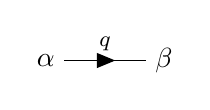
\begin{tikzpicture}[baseline={([yshift=-0.7ex]current bounding box.center)}]
		\begin{feynman}
			\vertex (a) {$\alpha$};
			\vertex [right=of a] (b) {$\beta$};
			\diagram* {
				(a) -- [fermion, edge label={\footnotesize$q$}] (b),
			};
		\end{feynman}
	\end{tikzpicture}
	\quad $\, = \bigg(\cfrac{i(\cslashed{q} + m)}{q^2 - M^2 + i\varepsilon}\bigg)_{\alpha\beta}$ 
    \\[1em]
    Photons: \qquad \;
	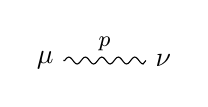
\begin{tikzpicture}[baseline={([yshift=-0.7ex]current bounding box.center)}]
		\begin{feynman}
			\vertex (a) {$\mu$};
			\vertex [right=of a] (b) {$\nu$};
			\diagram* {
				(a) -- [boson, edge label={\footnotesize$p$}] (b),
			};
		\end{feynman}
	\end{tikzpicture}
	\quad $\, = -i \cfrac{\eta_{\mu\nu}}{p^2 + i\epsilon}$ 
    \\[1em]
	\item External lines (on-shell particles)  \\
    % \\[1.5em]
    % % \hspace*{-\leftmargini}
    % \begin{minipage}{0.99\textwidth}
    \begin{tabbing}
    Incoming fermions: 
    \hspace*{1.5cm}
    \=
    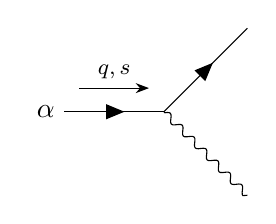
\begin{tikzpicture}[baseline={([yshift=-0.8ex]current bounding box.center)}]
        \begin{feynman}
            \vertex (a) {$\alpha$};
            \vertex [right=of a] (b);
            \vertex [above right=of b] (f1);
            \vertex [below right=of b] (f2);
            \diagram* {
                (a) -- [fermion, momentum={\footnotesize$q, s$}] (b),
                (b) -- [fermion] (f1),
                (b) -- [boson] (f2),
            };
        \end{feynman}
    \end{tikzpicture}
    \hspace*{0.4cm}
    \=
    $ = u^s_\alpha(q)$
    \\[1.5em]
    Incoming antifermions: 
    \>
    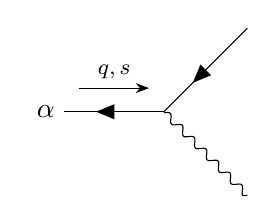
\begin{tikzpicture}[baseline={([yshift=-0.8ex]current bounding box.center)}]
        \begin{feynman}
            \vertex (a) {$\alpha$};
            \vertex [right=of a] (b);
            \vertex [above right=of b] (f1);
            \vertex [below right=of b] (f2);
            \diagram* {
                (a) -- [anti fermion, momentum={\footnotesize$q, s$}] (b),
                (b) -- [anti fermion] (f1),
                (b) -- [boson] (f2),
            };
        \end{feynman}
    \end{tikzpicture}
    \>
    $ = \bar v^s_\alpha(q)$
    \\[1.5em]
    Outgoing fermions: 
    \>
    % \hspace*{1.5cm}
    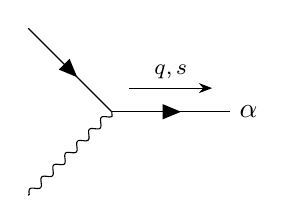
\begin{tikzpicture}[baseline={([yshift=-0.8ex]current bounding box.center)}]
        \begin{feynman}
            \vertex (a);
            \vertex [right=of a] (b) {$\alpha$};
            \vertex [above left=of a] (f1);
            \vertex [below left=of a] (f2);
            \diagram* {
                (f1) -- [fermion] (a),
                (f2) -- [boson] (a),
                (a) -- [fermion, momentum={\footnotesize$q, s$}] (b),
            };
        \end{feynman}
    \end{tikzpicture}
    \>
    $ = \bar{u}^s_\alpha(q)$
    \\[1.5em]
    Outgoing antifermions: 
    \>
    % \hspace*{1.5cm}
    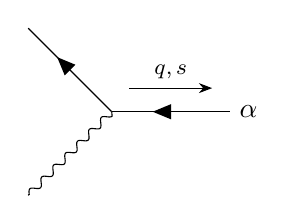
\begin{tikzpicture}[baseline={([yshift=-0.8ex]current bounding box.center)}]
        \begin{feynman}
            \vertex (a);
            \vertex [right=of a] (b) {$\alpha$};
            \vertex [above left=of a] (f1);
            \vertex [below left=of a] (f2);
            \diagram* {
                (f1) -- [anti fermion] (a),
                (f2) -- [boson] (a),
                (a) -- [anti fermion, momentum={\footnotesize$q, s$}] (b),
            };
        \end{feynman}
    \end{tikzpicture}
    \>
    $ = v^s_\alpha(q)$
    \\[1.5em]
    Incoming photons: 
    \>
    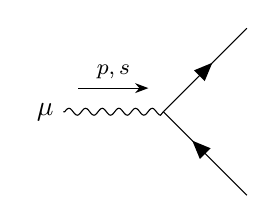
\begin{tikzpicture}[baseline={([yshift=-0.8ex]current bounding box.center)}]
        \begin{feynman}
            \vertex (a) {$\mu$};
            \vertex [right=of a] (b);
            \vertex [above right=of b] (f1);
            \vertex [below right=of b] (f2);
            \diagram* {
                (a) -- [boson, momentum={\footnotesize$p, s$}] (b),
                (b) -- [fermion] (f1),
                (b) -- [anti fermion] (f2),
            };
        \end{feynman}
    \end{tikzpicture}
    \>
    $ = \epsilon^\lambda_\mu$
    \\[1.5em]
    Outgoing photons: 
    \>
    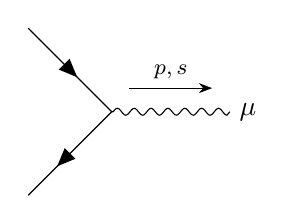
\begin{tikzpicture}[baseline={([yshift=-0.8ex]current bounding box.center)}]
        \begin{feynman}
            \vertex (a);
            \vertex [right=of a] (b) {$\mu$};
            \vertex [above left=of a] (f1);
            \vertex [below left=of a] (f2);
            \diagram* {
                (f1) -- [fermion] (a),
                (f2) -- [anti fermion] (a),
                (a) -- [boson, momentum={\footnotesize$p, s$}] (b),
            };
        \end{feynman}
    \end{tikzpicture}
    \>
    $ = \epsilon^{\lambda*}_\mu$
    \\
    \end{tabbing}
	\item Impose momentum conservation at each vertex.
	\item Integrate over the momentum $k$ flowing through each loop.
	\item Figure out the sign based on statistics. 
\end{enumerate}
	% QED has proven over the last century to be one of our most precise and successful theories;
	% we will look at some of its important processes in the next chapter.
\end{definition}

% \subsubsection{A scattering example and the Coulomb potential}

These Feynman rules can be applied to simple tree-level processes similarly to Yukawa theory (see Sections~\ref{sec:01_qft_interactions_feynman} and~\ref{sec:01_qft_spinors_feynman}).
These include several important processes such as electron-electron scattering $e^-e^- \rightarrow e^-e^-$ via a virtual photon, Compton scattering $\gamma e^- \rightarrow \gamma e^-$, electron-positron annihilation $e^+e^- \rightarrow \gamma\gamma$, and electron-positron (or Bhabha) scattering $e^+e^- \rightarrow e^+e^-$.
% We will discuss just one example, of electron-electron scattering $e^-e^- \rightarrow e^-e^-$, 
The former (and its variations with other charged particles) is what we generally experience as electromagnetism, and can recover the Coloumb potential in the non-relativistic limit.


\subsection{Yang-Mills Theory}
\label{sec:01_qft_gt_yangmills}

Following the remarkable success of QED and GR, a generalization of such gauge theories to \textit{non-abelian} symmetries was proposed by Chen Ning Yang and Robert Mills in 1953~\cite{Yang:1954ek}, today referred to as \textit{Yang-Mills} theories.
These theories picked up steam in the 1960s when the concept of spontaneous symmetry breaking was developed to give mass to the gauge bosons (Section~\ref{sec:01_qft_higgs}) and it was realized that both the weak and strong interactions can be described by \SU[2] and \SU[3] Yang-Mills theories, respectively.
They are hence a cornerstone of the SM, and we will now briefly outline their construction, generalizing the \UU[1] gauge symmetry from the previous section.
% Since then, Yang-Mills theories have become the cornerstone of the SM, with the electroweak and strong interactions described by \suu and \SU[3] Yang-Mills theories, respectively.
% We now briefly outline the generalization of \UU[1] gauge theories to these non-abelian gauge groups, leaving discussions of the many subtleties related to quantization and anomalies to dedicated texts such as Tong GT~\cite{TongGT} and Peskin and Shroeder~\cite{Peskin:1995ev}.

\subsubsection{Non-abelian gauge transformations}

In Yang-Mills theory, we allow non-gauge fields to transform locally under \textit{any} Lie group $G$, in an arbitrary representation $R$ of the group (generally, in the SM, $R$ is either the fundamental or trivial representation).
This means the fields $\psi$ are actually vectors of $\dim(R)$ (on top of their usual spinor or $4$-vector indices etc.), and transform as:
\begin{equation}
	\label{eq:01_qft_gt_yangmills_transformation}
	\psi(x) \rightarrow \psi'(x) = e^{i\alpha^a(x)T_R^a}\psi(x) \equiv V(x) \psi(x),
\end{equation}
where $T_R^a$ are the generators of $G$ in the representation $R$ and $V(x) = e^{i\alpha^a(x)T_R^a}$ is the gauge transformation.
To construct a $G$-invariant Lagrangian, we again need to define a covariant derivative with gauge fields $A_\mu^a$ connecting the local transformations of $\psi$ across spacetime:
\begin{equation}
	\label{eq:01_qft_gt_yangmills_dmu}
	D_\mu\psi = (\partial_\mu - igA_\mu^aT_R^a)\psi.
\end{equation}
Observe that we must have as many gauge fields as there are group generators to counter all possible gauge transformations $V(x)$; i.e., there are $\dim(G)$ $A_\mu$s, living in the \textit{adjoint} representation of $G$ (see Chapter~\ref{sec:01_symmetries_so3}).
The gauge field is often represented more conveniently as a ``Lie-algebra-valued'' field (i.e., as an object in the Lie algebra):
\begin{equation}
	\label{eq:01_qft_gt_yangmills_gauge_field}
	A_\mu \equiv A_\mu^aT^a.
\end{equation}

We can derive how $A_\mu$ transforms by requiring the covariant derivative to transform identically to $\psi$ (the same as in the abelian case):\footnote{For a detailed derivation see e.g. Ricardo Matheus' QFT Lectures~\cite{MatheusQFT} Part 34.}
\begin{equation}
	\label{eq:01_qft_gt_yangmills_dmu_transformation}
	D_\mu\psi \rightarrow D'_\mu\psi = (\partial_\mu - igA_\mu')V\psi \mustequal VD_\mu\psi(x),
\end{equation}
where $g$ is the coupling constant.
One can check this is satisfied for the transformed gauge field:
\begin{equation}
	\label{eq:01_qft_gt_yangmills_gauge_transformation_A}
	 A_\mu' = V A_\mu V^{-1} - \frac{i}{g}(\partial_\mu V)V^{-1}.
\end{equation}
For infinitesimal gauge transformations $V \simeq 1 + i\alpha^aT_R^a$, this can be written in terms of the components as:
\begin{equation}
	\label{eq:01_qft_gt_yangmills_gauge_transformation_A_infinitesimal}
	 A_\mu^{'a}T^a = A_\mu^aT^a + \frac{1}{g}\partial_\mu\alpha^aT^a + i A_\mu^a\alpha^b[T^b, T^a] = A_\mu^aT^a + \frac{1}{g}\partial_\mu\alpha^aT^a - f^{abc}A_\mu^a\alpha^bT^c,
\end{equation}
where $f^{abc}$ are the structure constants of the Lie algebra of $G$.
The second term represents the gauge transformation, same as in the abelian case, while the third term is new and is the transformation property for a field in the adjoint representation.
% In the abelian case, $f^{abc} = 0$ and we reproduce the \UU[1] transformation, Eq.~\ref{eq:01_qft_gt_maxwell_gauge}.

\subsubsection{The field strength tensor}

The final piece we need for the Lagrangian is a gauge-invariant kinetic term for the gauge fields, generalizing the electromagnetic field strength tensor $F_{\mu\nu}$.
We can construct this, as in the abelian case, using the commutator of covariant derivatives:
\begin{equation}
	\label{eq:01_qft_gt_yangmills_field_strength}
	F_{\mu\nu} \equiv \frac{i}{g}[D_\mu, D_\nu] = (\partial_\mu A_\nu^a - \partial_\nu A_\mu^a) - ig[A_\mu, A_\nu].
\end{equation}
Again, this reduces to the E\&M tensor for an abelian symmetry, where the commutator term is $0$.
In the non-abelian case, the commutator term adds new \textit{self-interaction} terms to the gauge fields.
One can check that $F_{\mu\nu}$ transforms as:
\begin{equation}
	\label{eq:01_qft_gt_yangmills_field_strength_transformation}
	F_{\mu\nu} \rightarrow V F_{\mu\nu} V^{-1},
\end{equation}
or, infinitesimally, in terms of components as:
\begin{equation}
	\label{eq:01_qft_gt_yangmills_field_strength_transformation_infinitesimal}
	F_{\mu\nu}^aT^a \rightarrow F_{\mu\nu}^aT^a + f^{abc}F_{\mu\nu}^b\alpha^cT^a,
\end{equation}
which we can recognize as the transformation of a field in the adjoint representation (Eq.~\ref{eq:01_qft_gt_yangmills_gauge_transformation_A_infinitesimal} without the gauge transformation term).

Clearly, for non-abelian theories, the field-strength tensor alone, or even $F_{\mu\nu}F^{\mu\nu}$, is no longer gauge-invariant; however, its \textit{trace} is:
\begin{equation}
	\label{eq:01_qft_gt_yangmills_trace_field_strength_transformation}
	\tr{F_{\mu\nu}F^{\mu\nu}} \rightarrow \tr{V F_{\mu\nu}V^{-1} V F^{\mu\nu} V^{-1}} = \tr{F_{\mu\nu}F^{\mu\nu}}
\end{equation}
using the cyclic property of the trace, providing us with a gauge-invariant kinetic term for the gauge fields.
In terms of components, this is:
\begin{equation}
	\label{eq:01_qft_gt_yangmills_trace_field_strength}
	\tr{F_{\mu\nu}F^{\mu\nu}} = F_{\mu\nu}^aF^{a\mu\nu}\, \tr{T^aT^a}
\end{equation}
The value of $\tr{T^aT^a}$ is a normalization constant that is conventionally chosen to be $\frac{1}{2}$ for the fundamental representation.
Expanding out $(F_{\mu\nu}^a)^2$ gives us cubic and quartic self-interaction terms for the gauge fields.

\subsubsection{The Yang-Mills Lagrangian}

Combining all of the above, we have the gauge-invariant Yang-Mills Lagrangian:
\begin{equation}
	\label{eq:01_qft_gt_yangmills_lagrangian}
	\mathcal L = -\frac{1}{2}\tr{F_{\mu\nu}F^{\mu\nu}} + \bar\psi(i\cslashed D - m)\psi,
\end{equation}
or, in explicit, component form:
\begin{equation}
	\label{eq:01_qft_gt_yangmills_lagrangian_explicit}
	\mathcal L = -\frac{1}{4}F_{\mu\nu}^aF^{a\mu\nu} + \bar\psi_i[\delta_{ij}(i\cslashed \partial_\mu - m) + g\cslashed A^aT_{ij}^a]\psi_j,
\end{equation}
where the indices $i$ and $j$ are running over the fermion fields in the representation $R$.
Note again that a mass term $m^2A_\mu^aA^{a\mu}$ would violate gauge invariance without the Higgs mechanism.

Interestingly, despite the extra self-interaction terms, there remains only one free parameter in the theory: the coupling constant $g$.
This is why the SM, despite its apparent complexity, has so few free parameters, particularly in the ``gauge sector'' (the majority of free parameters are related to couplings in the \textit{Higgs} sector).
It is also worth emphasizing that the primary difference \textit{physically} between abelian and non-abelian gauge theories is that the gauge bosons are charged under the gauge group in the latter (and, hence, self-interact).

% On the other hand, there is a new term which \textit{is} possible, 


\subsubsection{Quantum Yang-Mills Theory}
\label{sec:01_qft_gt_ymquant}

The form of the quantized gauge fields in Yang-Mills are similar to the \UU[1] case, except now with the extra adjoint representation indices.
The process of quantization and deriving the propagator, however, is considerably more involved for non-abelian theories.
The core idea of adding an $R_\xi$ gauge-fixing term to the Lagrangian is similar, but due to the gauge fields' non-trivial transformation property, the proper treatment necessitates the introduction of imaginary internal particles called \textit{Faddeev-Popov ghosts} to cancel gauge-dependent terms.
Somewhat similar to virtual particles, these ghosts are purely mathematical artifacts required to maintain gauge- and Lorentz-invariance of the quantized theory.
The full details of this process can be found in e.g. Peskin and Shroeder~\cite{Peskin:1995ev} Chapter 16; the upshot is simply some extra Feynman rules involving ghost particles in the theory.

The new Feynman rules for \textit{non-abelian Yang-Mills} theories are shown in Figure~\ref{fig:01_qft_gt_yangmills_feynman}.
The gauge bosons are conventionally referred to as ``gluons'' but these rules are general.
Note the cubic and quartic gauge boson vertices, as well as the ghost particle ($c$) diagrams, unique to non-abelian theories.
The phenomenology of Yang-Mills theories in the SM will be discussed in the next chapter.

\begin{figure}[ht!]
	\centering
	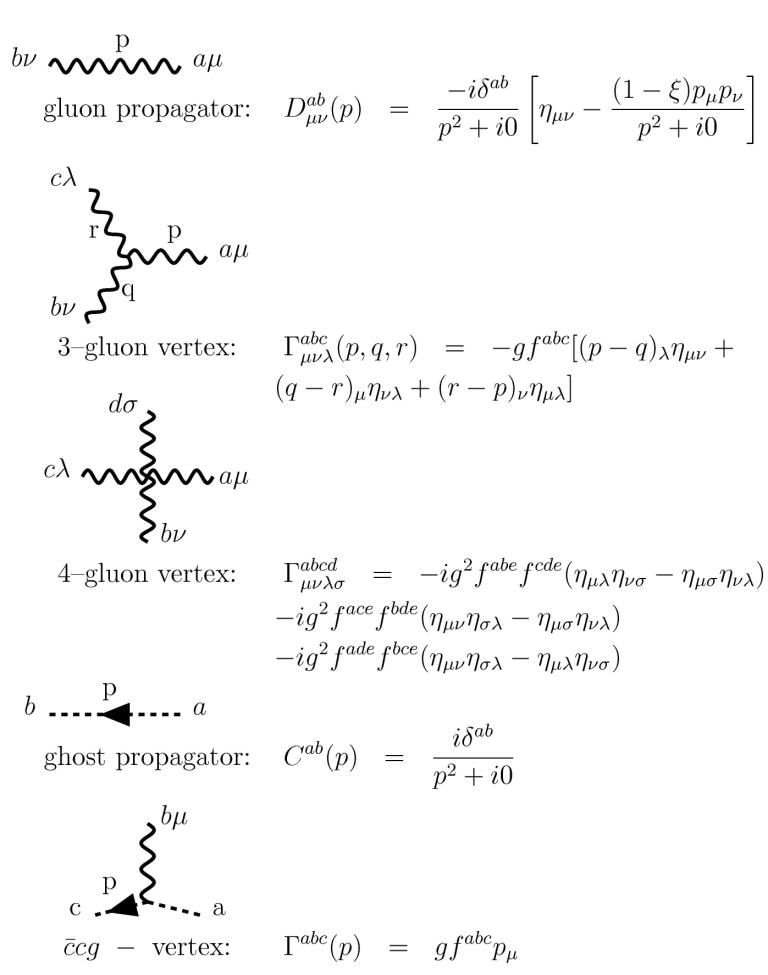
\includegraphics[width=0.8\textwidth]{figures/01-SM-02-QFT/Feynman/yangmills}
	\caption{Feynman rules unique to non-abelian Yang-Mills theories, reproduced from Ref.~\cite{enwiki:1243569653}.}
	\label{fig:01_qft_gt_yangmills_feynman}
\end{figure}


\subsection{Running couplings and asymptotic freedom}
\label{sec:01_qft_gt_asymptotic}

As discussed briefly in Section~\ref{sec:01_qft_interactions}, in order to handle divergences from higher order ``loop'' diagrams in perturbation theory, a class of mathematical techniques called \textit{renormalization} is employed.
A perhaps surprising physical consequence of this is that parameters of the theory are dependent on the energy scale at which they are probed.
Their dependence is described the \textit{renormalization group equations} or \textit{flow}.

The renormalization group is an extremely deep subject with applications in many areas of physics.
The most relevant result for us is the \textit{running} of the coupling constants in gauge theories --- i.e., the strength of the corresponding forces as a function of the energy scale.
This is shown for the relevant \UU[1], \SU[2], and \SU[3] gauge symmetries of the SM in Figure~\ref{fig:01_qft_running}.

\begin{figure}[ht]
	\centering
	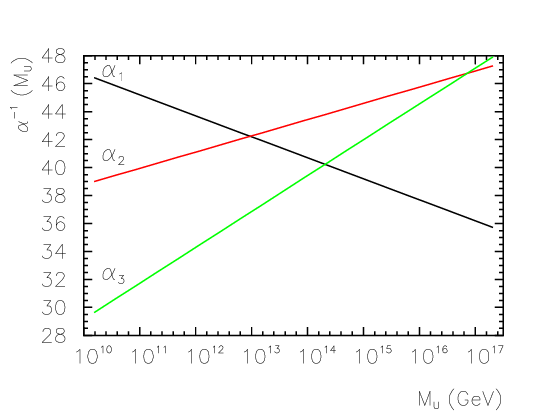
\includegraphics[width=0.8\textwidth]{figures/01-SM-03-SM/qcd/Running-couplings-in-the-standard-model.png}
	\caption{The running of the inverse strength of the SM coupling constants, with the strong coupling constant (\SU[3]) in green, weak (\SU[2]) in red, and electromagnetic (\UU[1]) in black, reproduced from Ref.~\cite{Dias2004}.}
	\label{fig:01_qft_running}
\end{figure}

We see firstly that the electromagnetic interaction strength increases with energy scale.
Physically, this is understood through the \textit{vacuum polarization} via virtual electron-positron pair creation, which ``screen'' the electric charges of real particles more effectively at longer distances, thereby weakening the force.\footnote{Interestingly, QED has a Landau pole: a finite value of the energy scale for which the interaction strength is infinite. However, this value is so high ($10^{286} \GeV$) as to have no practical consequence, and likely points to the breakdown of perturbation theory, that is used to derive the running coupling, at such a scale.}

A notable, Nobel-prize winning, 1973 result of Frank Wilczek, David Gross, and David Politzer, however, was an inverse dependence on energy for non-abelian gauge theories~\cite{Politzer:1973fx, Gross:1973id}, as shown for the \SU[2] and \SU[3] couplings in Figure~\ref{fig:01_qft_running}.\footnote{Technically, this depends on the gauge group and the number of fermions in the theory; for both the weak and strong forces, this number is sufficiently small (see e.g. Peskin and Shroeder~\cite{Peskin:1995ev} Chapter 16).}
This phenomenon is called \textit{asymptotic freedom}, as in the high energy limit the theory is effectively one of free particles.
It is a notable feature of the strong force, as will be discussed in Chapter~\ref{sec:01_sm_qcd}.


\section{The ABEGHHK (Higgs) mechanism}
\label{sec:01_qft_higgs}

As highlighted in the previous section, gauge bosons in pure Yang-Mills theories are massless.
This is in conflict, however, with the short observed range of the weak force, implying massive mediatory bosons.
To resolve this, a series of work in the early 1960s by Anderson, Brout, Englert, Guralnik, Hagen, Higgs, and Kibble (ABEGHHK) yielded a mechanism to give mass to the gauge bosons without violating gauge invariance~\cite{Anderson:1963pc, Englert:1964et, Higgs:1964pj, Guralnik:1964eu}, based on the concept of \textit{spontaneous symmetry breaking} developed by Nambu~\cite{Nambu:1961tp, Nambu:1961fr} and others.

By 1970, Glashow, Salam, Weinberg and others were able to use this mechanism to formulate a combined theory of weak and electromagnetic interactions, known as ``electroweak'' or Weinberg-Salam theory~\cite{Glashow:1959wxa, Salam:1968rm, Weinberg:1967tq}.
Electroweak unification has been one of the most significant breakthroughs in theoretical physics with several Nobel prizes cumulatively awarded for these developments.

In this section we outline the ABEGHHK mechanism --- commonly (but reductively) referred to as the ``Higgs mechanism'' --- first for an abelian gauge theory in Section~\ref{sec:01_qft_higgs_abelian} and then for non-abelian gauge theories~\ref{sec:01_qft_higgs_nonabelian} like the SM.

\subsection{The abelian Higgs mechanism}
\label{sec:01_qft_higgs_abelian}

The Higgs mechanism is based on the idea of spontaneous symmetry breaking (SSB), where the ground states of a physical system violate the overall symmetry.
The classic example is the so-called ``sombrero'' potential for a complex scalar field $\phi$:
\begin{equation}
	\label{eq:01_qft_higgs_potential}
	V(\phi) = -\frac{\lambda}{2}(\abs{\phi}^2 - v^2)^2,
\end{equation}
for constants $\lambda$ and $v$, shown in Figure~\ref{fig:01_qft_higgs_potential}.
The potential has is symmetric under a \UU[1] transformation of $\phi \rightarrow e^{i\alpha}\phi$, but any specific ground state of $\abs{\phi} = v$ will break this symmetry, as shown in the figure.
SSB is a crucial concept in physics, with several applications in condensed matter and particle physics, including chiral symmetry breaking in QCD (see e.g. Tong SM~\cite{TongSM} Chapter 3.2).

\begin{figure}[ht!]
	\centering
	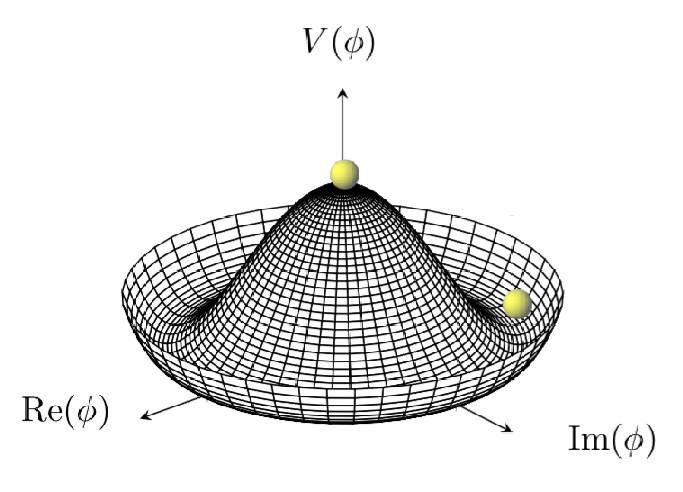
\includegraphics[width=0.7\textwidth]{figures/01-SM-02-QFT/sombrero_potential.png}
	\caption{The ``sombrero'' potential for the Higgs field, reproduced from Ref.~\cite{Duff:2020wmn}.
	An initial state and a ground state breaking the \UU[1] symmetry are represented by the green balls at the top and bottom of the potential, respectively.}
	\label{fig:01_qft_higgs_potential}
\end{figure}

The Higgs mechanism is an application of SSB to \textit{gauge} symmetries.
The interpretation here of SSB a bit fiddly since, as emphasized above, gauge symmetries are not physical and cannot be spontaneously broken;\footnote{This is an implication of Elitzur's theorem~\cite{Elitzur:1975im}.} what actually breaks is the corresponding \textit{global} symmetry, as we outline below.

Consider our QED Lagrangian for a complex scalar field $\phi$ with the above potential:
\begin{equation}
	\label{eq:01_qft_higgs_lagrangian}
	\mathcal L = -\frac{1}{4}F_{\mu\nu}F^{\mu\nu} + (D_\mu\phi)^\dagger D^\mu\phi + \frac{\lambda}{2}(\abs{\phi}^2 - v^2)^2.
\end{equation}
As before, this Lagrangian possesses a \UU[1] gauge symmetry; however, this symmetry is ``broken'' by a particular ground state $\phi = v e^{i\delta}$ (we can take $\delta = 0$ WLOG).
The fluctuations around the ground state can be parametrized as:
\begin{equation}
	\label{eq:01_qft_higgs_fluctuations}
	\phi(x) = (v + \sigma(x))e^{i\theta(x)},
\end{equation}
where $\sigma$ and $\theta$ are two real fields.
Plugging this into the Lagrangian gives us:
\begin{equation}
	\label{eq:01_qft_higgs_fluctuations_lagrangian}
	\mathcal L = -\frac{1}{4}F_{\mu\nu}F^{\mu\nu} + \partial_\mu\sigma \partial^\mu\sigma + (v + \sigma)^2(\partial_\mu\theta - e A_\mu)(\partial^\mu\theta - e A^\mu) - \lambda(2v^2\sigma^2 + 2 v\sigma^3 + \frac{\sigma^4}{4}).
\end{equation}
We see first that $\sigma$ can be interpreted as a normal scalar quantum field, with a quadratic mass term with $m_\sigma^2 = 2\lambda v^2$.
The $\theta$ term is a bit more unusual;\footnote{In a non-gauge-theory, the $\theta$ field would be considered a massless ``Goldstone boson'' resulting from the spontaneously breakdown of the symmetry.}
it only appears in the combination $\partial_\mu\theta - e A_\mu$.
Hence, we can simply redefine the gauge field as $A_\mu' \equiv A_\mu + \frac{1}{e}\partial_\mu\theta$, allowing it to ``absorb'' this DoF.
Note that this takes the form of a gauge transformation of $A_\mu$ and thus does not affect the field strength tensor $F_{\mu\nu}$.
The resulting Lagrangian is then:
\begin{equation}
	\label{eq:01_qft_higgs_fluctuations_lagrangian_final}
	\mathcal L = -\frac{1}{4}F_{\mu\nu}F^{\mu\nu} + \partial_\mu\sigma \partial^\mu\sigma + e^2(v + \sigma)^2A_\mu'A^{'\mu} - \lambda(2v^2\sigma^2 + 2 v\sigma^3 + \frac{\sigma^4}{4}),
\end{equation}
where we now have a mass term for the ``gauge boson'', $m_A^2 = 2e^2 v^2$!

\subsection{The non-abelian Higgs mechanism}
\label{sec:01_qft_higgs_nonabelian}

There is an analogous mechanism for a non-abelian gauge symmetry, as in the SM.
One crucial difference is that the symmetry may only partially break from the gauge group $G$ to a subgroup $H$ (for example from \SU[2] to a \UU[1]).
In this case, the gauge bosons corresponding to the generators of $G$'s broken symmetries acquire mass as above, while the generators of $H$ remain massless Goldstone bosons; as we will see in Chapter~\ref{sec:01_sm_ew}, in the SM these correspond to the massive $W^\pm$ / $Z$ bosons and the massless photon, respectively.
See e.g. Tong SM~\cite{TongSM} Chapter 2.3.3 for an example.


% \section{Brief encounters with renormalization}
% \label{sec:01_qft_renormalization}

%  - perturbation theory leads to infinite integrals at high orders, theory is considered renormalizable if these infinities are canceled or made finite by imposing a cut-off energy scale beyond which the theory is not valid
%  - implicitly, this means that physical parameters of the theory are not fixed, but depend on the energy scale at which they are measured --- the coupling constants, in particular, are considered to "run" with the energy scale.

% % \begin{center}
%   \centering
%   \noindent
%   \textit{If I could remember the names of all these particles, I'd be a botanist.} --- Enrico Fermi
% \end{center}

\chapter{The Standard Model of Particle Physics}
\label{sec:01_sm}

\begin{center}
	\centering
	\noindent
	\textit{Before I came here, I was confused about this subject. Having listened to your lecture, I am still confused. But on a higher level.} --- Enrico Fermi\footnote{Also an accurate representation of my understanding of the SM before and after my PhD.}
\end{center}


\begin{figure}
	\centering
	\captionsetup{justification=centering}
	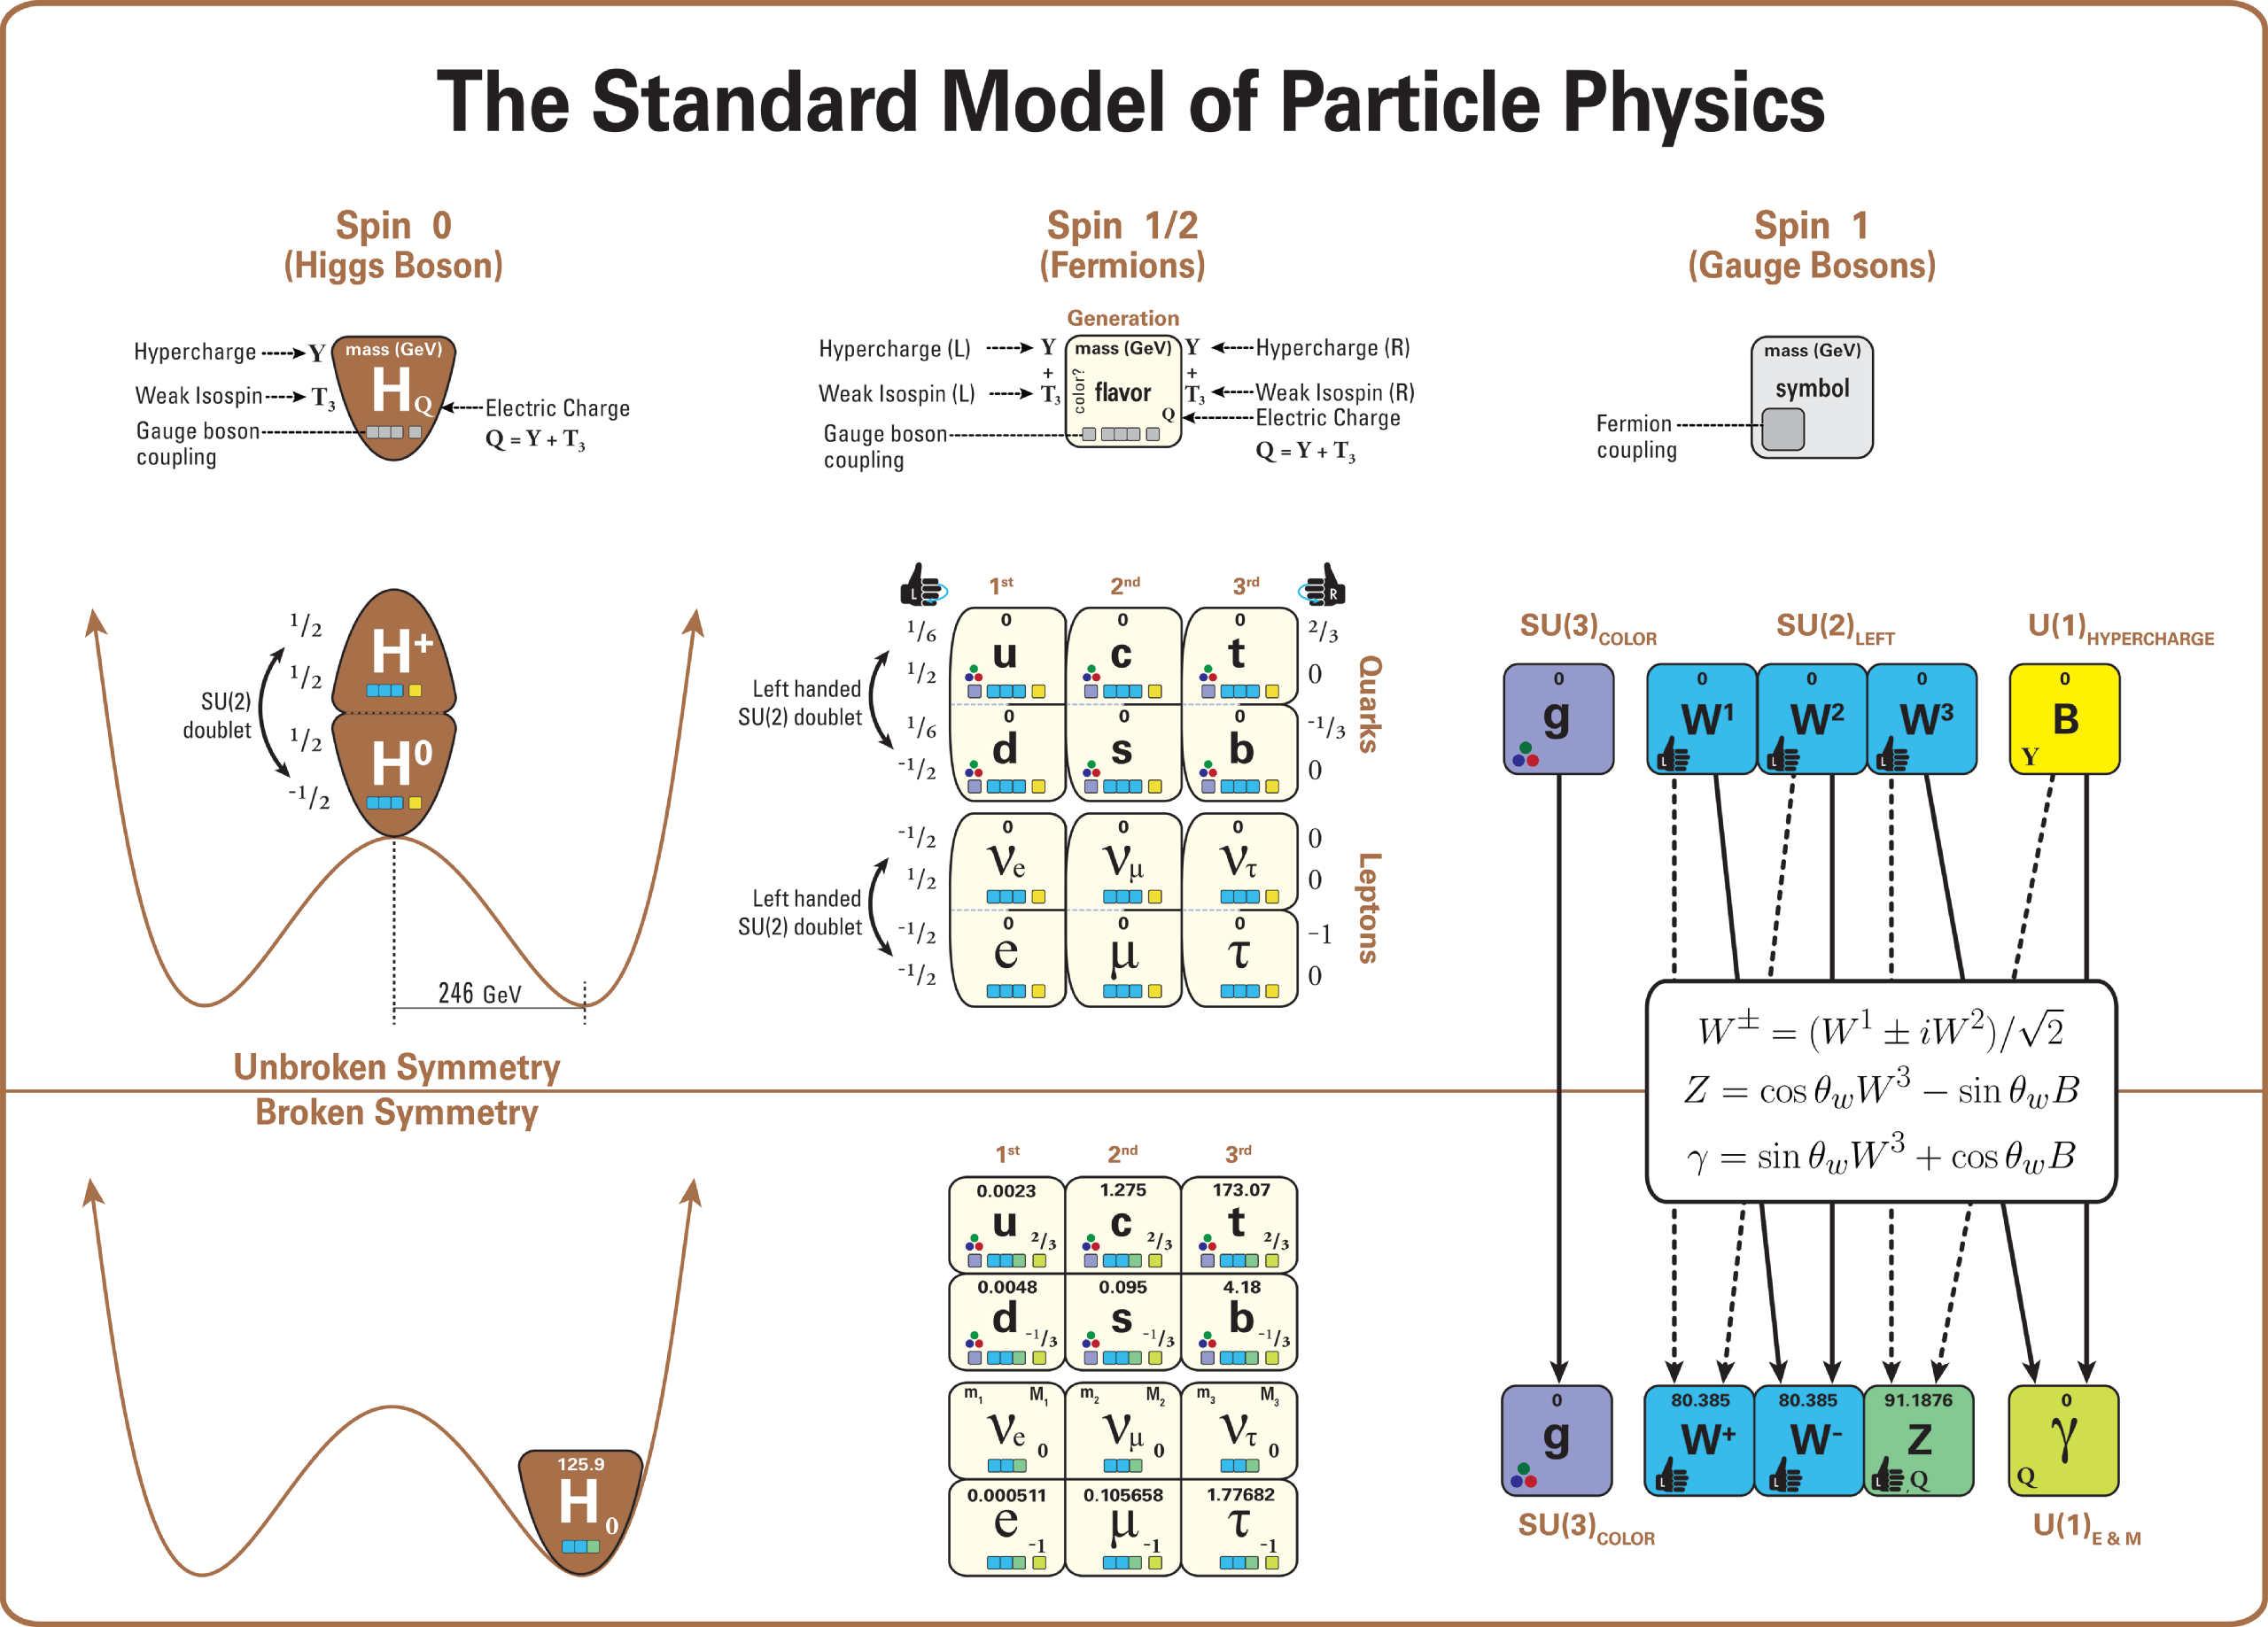
\includegraphics[width=\textwidth]{figures/01-SM-03-SM/Standard_Model_Of_Particle_Physics--Most_Complete_Diagram.png}
	\caption{A graphical summary of the SM, reproduced from Ref.~\cite{SMMostCompleteDiagram}.}
	\label{fig:01_sm_summary}
\end{figure}

We are now ready to describe the standard model (SM)!
It is a renormalizable, quantum Yang-Mills theory, and is illustrated nicely in Figure~\ref{fig:01_sm_summary}.
Before electroweak symmetry breaking (EWSB) --- a form of spontaneous symmetry breaking (SSB) --- it possessed the gauge symmetry $\SU[3]_{\mathrm{C}} \times \SU[2]_{\mathrm{L}} \times \UU[1]_{\mathrm{Y}}$, with $C$, $L$, and $Y$ standing for color, left, and hypercharge, respectively.
%  (their significance will be explained in the following sections).
These three groups correspond to the strong, weak, and electromagnetic forces, with eight, three, and one generators or gauge bosons, respectively.
The relative strengths of each interaction, as well as gravity's, are shown in Table~\ref{tab:01_sm_coupling_constants}, based on the equivalent of the fine structure constant of each force, $\alpha_f = \cnicefrac{g_f}{4\pi}$, where $g_f$ is the respective coupling constant.

The SM contains six fermions charged and uncharged under the $\SU[3]_{\mathrm{C}}$ symmetry each, called the ``quarks'' and ``leptons'', respectively.
% --- the ``quarks'' --- and six fermions uncharged --- the ``leptons''.
The left-handed fermions live as pairs in $\SU[2]_{\mathrm{L}}$ doublets, while the right-handed fermions in singlets.
The six types of fermions are referred to as different ``flavors'', grouped into three generations as in Figure~\ref{fig:01_sm_summary}.

The SM also contains a complex scalar $\SU[2]_{\mathrm{Y}}$-doublet called the Higgs field, which is associated with EWSB.
As shown in Figure~\ref{fig:01_sm_summary}, it initially is at the center of a ``sombrero'' potential because of which, before EWSB, the gauge bosons, fermions, and the Higgs field are all massless.

% where the subscripts will be explained in the following sections, with massless gauge bosons and fermions a zero vacuum expectation value (VEV) for the Higgs field.
EWSB is hypothesized to have occurred during the electroweak epoch (see Figure~\ref{fig:00_timeline}), where the $\SU[2]_{\mathrm{L}} \times \UU[1]_{\mathrm{Y}}$ global symmetry broke to the $\UU[1]_{\mathrm{EM}}$ of QED.
Through this, the Higgs field obtained a non-zero vacuum expectation value (VEV), imbuing all the fermions, three of the gauge bosons, and the Higgs boson with mass --- a process referred to as the Higgs mechanism.
The outcome is the state of the universe and physics as we know it.

Of course, as outlined in the introduction, this picture does not explain myriad phenomena in fundamental physics, including dark matter, dark energy, baryon asymmetry, and neutrino masses.
This is why it is crucial to test the SM as rigorously and in as broad a phase space as possible, in order to identify any cracks that may point to new physics.

% The relative strength of each of their interactions is typically quantified by the equivalent of the fine structure constant for each force, $\alpha_f = \cnicefrac{g_f}{4\pi}$, where $g_f$ is the coupling constant.
% This is shown in Table~\ref{tab:01_sm_coupling_constants} for each force, as well as gravity for illustrative purposes.

\begin{table}[htbp]
    \centering
	\caption{Approximate magnitude of the strengths of the four fundamental forces at an energy scale of around 100\MeV.}
	\renewcommand{\arraystretch}{1.5}
    \begin{tabular}{ll}
        \toprule
        \textbf{Force} & \textbf{Strength}\\
        \midrule
        Electromagnetic &
        $\alpha_{\mathrm{EM}} \approx \frac{1}{137}$ \\
        Weak &
        $\alpha_W \approx \frac{1}{30}$\\
        Strong &
        $\alpha_s \approx 1$\\
        Gravity &
        $\alpha_G  \approx 10^{-38}$\\
        \bottomrule
    \end{tabular}
	\label{tab:01_sm_coupling_constants}
\end{table}

In this chapter, we will briefly walk through different areas of the SM.
Having discussed QED in Chapter~\ref{sec:01_qft_gt}, we begin with the remaining two fundamental interactions: quantum chromodynamics (Section~\ref{sec:01_sm_qcd}); and weak interactions and electroweak unification (Section~\ref{sec:01_sm_ew}).
% As we will see, the phenomenology of these forces is dictated by the ``running'' of their coupling constants; i.e., the dependence of the strength of the interactions on the energy scale at which they are probed, plotted in Figure~\ref{fig:01_sm_running}.
Finally, in Section~\ref{sec:01_higgs}, we will discuss the Higgs sector and pair production of the Higgs boson, which is the focus of this dissertation.


\section{Quantum chromodynamics}
\label{sec:01_sm_qcd}

Quantum chromodynamics (QCD) is a quantum Yang-Mills field theory describing the strong force, with the gauge group $\SU[3]$.
$\SU[3]$ has eight generators and, hence, eight gauge bosons ($G_\mu$) called gluons.
The only other elementary particles which interact with the strong force --- i.e., which don't live in the trivial representation of $\SU[3]$ --- are the quarks.
They live in the three-dimensional fundamental representation and thus possess three extra DoFs beyond vanilla spinors, which we call their ``color'' (hence, quantum \textit{chromo}dynamics).
The three orthogonal eigenstates in this representation are colloquially referred to as labeled red, green, and blue, and mathematically the quark fields ($q_\alpha$) labeled with extra color indices $i = 1, 2, 3$.

Putting this together, the QCD Lagrangian, with all the indices labeled explicitly is:
\begin{equation}
	\label{eq:01_sm_qcd_lagrangian}
	\mathcal L = -\frac{1}{4} G^a_{\mu\nu} G^{a\mu\nu} + \sum_{f = 1}^6 \bar q_{\alpha f i} [\delta_{ij}(i\cslashed \partial_{\alpha\beta} - m \delta_{\alpha\beta}) + g_s \cslashed G^a_{\alpha\beta} t_{ij}^a] q_{\beta f j}
\end{equation}
where $g_s$ is the strong coupling constant, $G^a_{\mu\nu} = \partial_\mu G^a_\nu - \partial_\nu G^a_\mu + g_s f^{abc} G^b_\mu G^c_\nu$ is the gluon field strength tensor, $f^{abc}$ are the structure constants of $\SU[3]$, $t^a$ are the generators of $\SU[3]$ in the fundamental representation, the sum over $f$ is running over the six flavors, and the indices $a$ and $i, j$ label the eight gluons and the three colors of quarks, respectively.
The six flavors of quarks have different masses and charges, as shown in Figure~\ref{fig:01_sm_qcd_quarks}.

\begin{figure}[ht]
	\centering
	\captionsetup{justification=centering}
	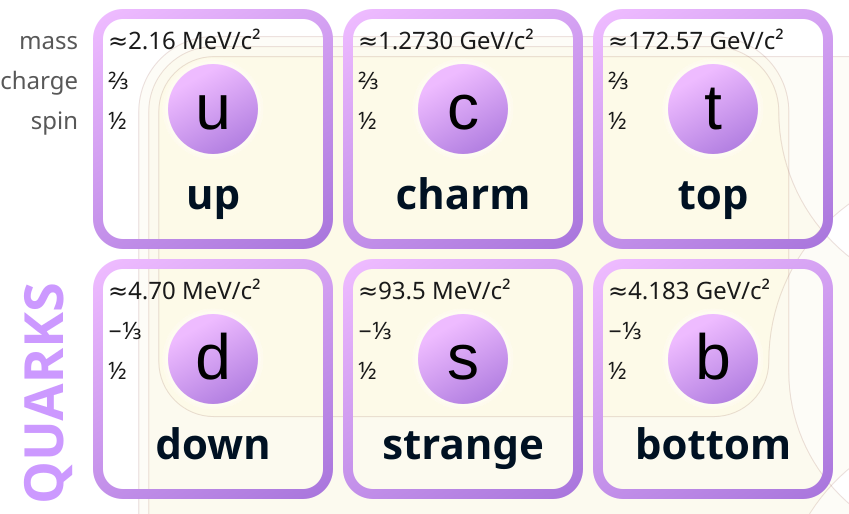
\includegraphics[width=0.5\textwidth]{figures/01-SM-03-SM/qcd/quarks.png}
	\caption{The quarks in the SM, reproduced from Ref.~\cite{enwiki:1238968997}.}
	\label{fig:01_sm_qcd_quarks}
\end{figure}

QCD is an extremely rich and complex theory due to its non-abelian gauge symmetry, the six different flavors of quarks, and the unique strength and running of its coupling, shown in Figure~\ref{fig:01_sm_qcd_running}.
Observe its property of weak coupling and asymptotic freedom at high energies, versus the extremely high $\mathcal O(1)$ value of $\alpha_s$ at low energies leading to the phenomenon of \textit{confinement}.
Note also that $\alpha_s$ appears to diverge in Figure~\ref{fig:01_sm_qcd_running} at around $200 \MeV$, a sign of perturbation theory breaking down. 
This $200 \MeV$ limit is considered the characteristic energy scale of QCD, $\Lambda_{\mathrm{QCD}}$.\footnote{The phenomenon of an energy scale arising from a dimensionless coupling constant  is known as \textit{dimensional transmutation} (see e.g. Tong SM~\cite{TongSM} Chapter 3).}

\begin{figure}[ht]
	\centering
	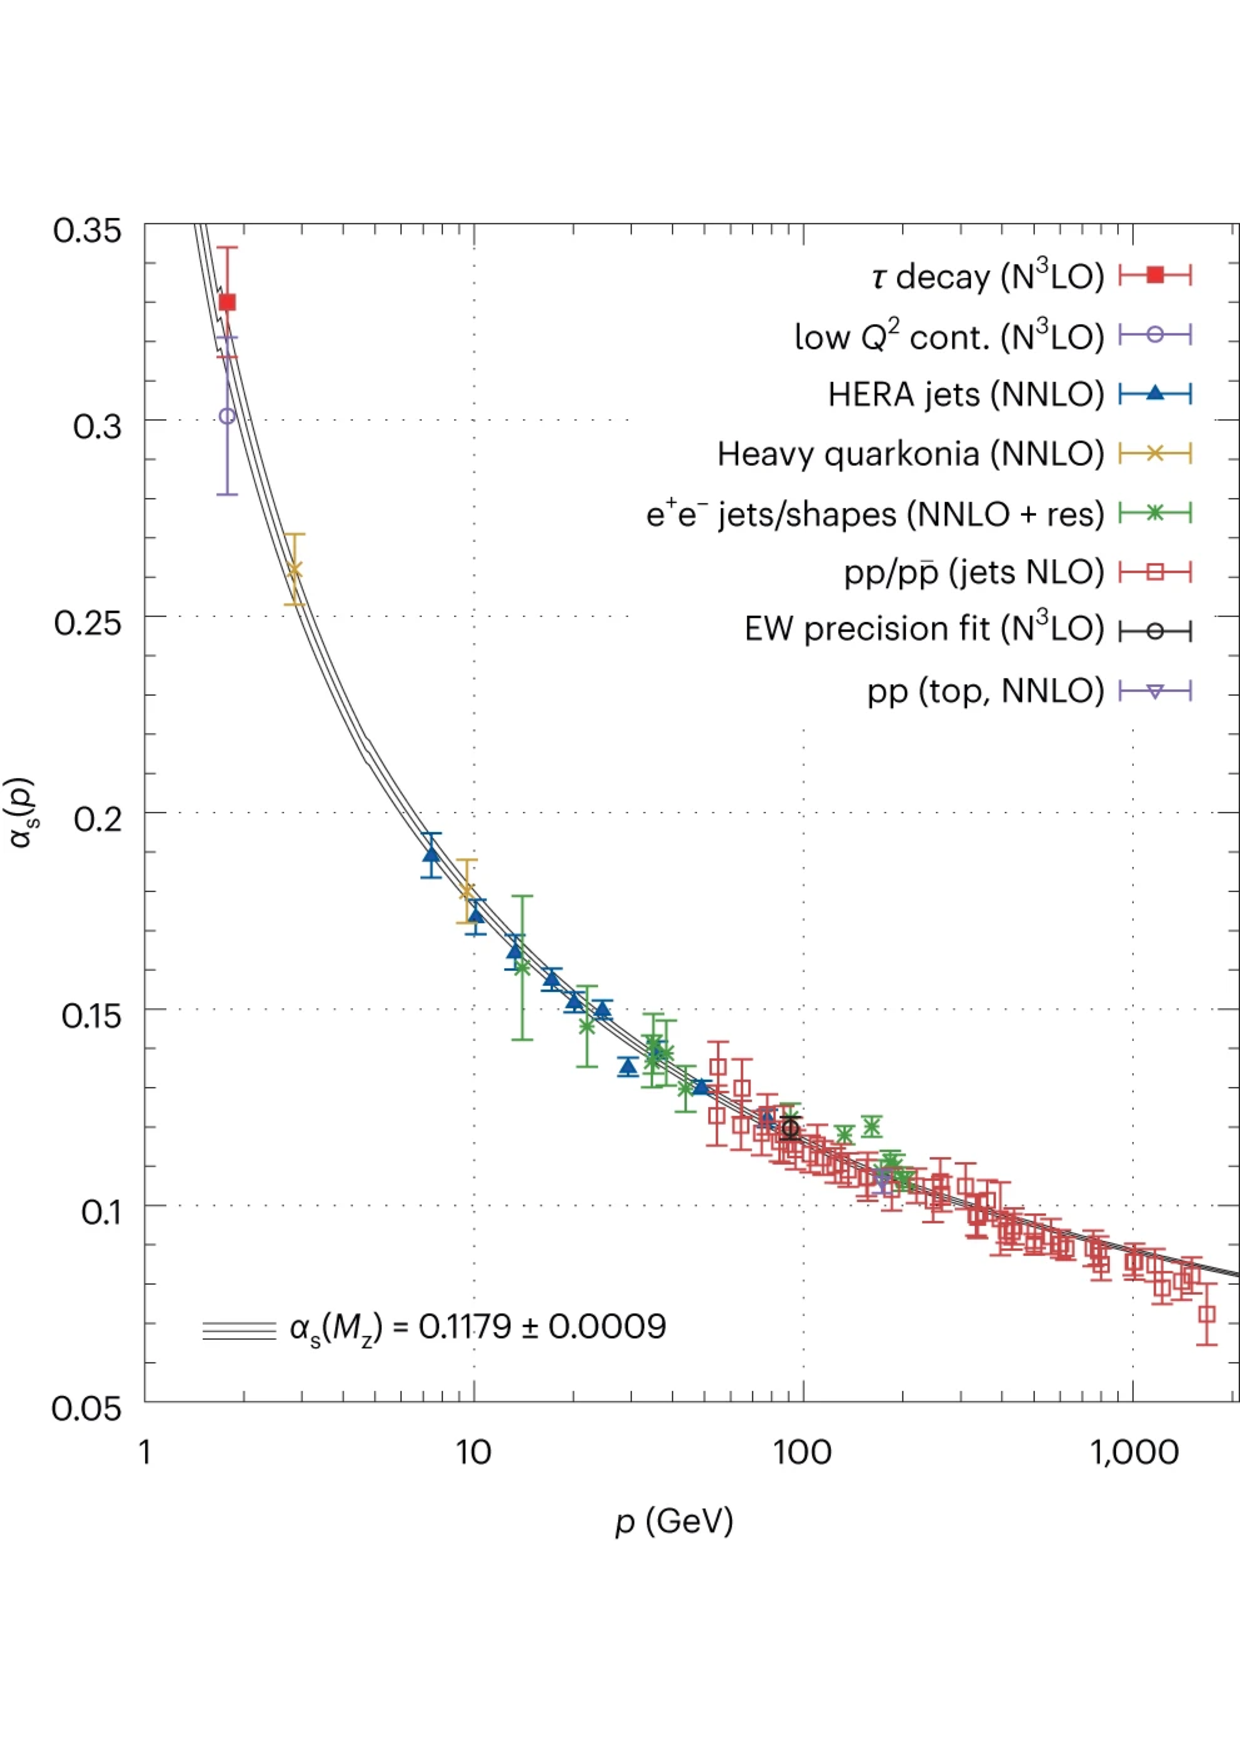
\includegraphics[width=0.5\textwidth]{figures/01-SM-03-SM/qcd/qcd_running}
	\caption{The theoretically predicted running of the strong coupling $\alpha_s = \cnicefrac{g_s^2}{4\pi}$ as a function of the energy scale along with experimental measurements, reproduced from Ref.~\cite{Boito:2023lzf}.}
	\label{fig:01_sm_qcd_running}
\end{figure}

The $\mathcal O(1)$ coupling strength means that the standard perturbative techniques we have discussed are not applicable at our usual energy scales; instead, we must rely on nonperturbative techniques such as numerical simulations of QCD on a discretized spacetime lattice (see e.g. Schwartz~\cite{Schwartz:2014sze} Chapter 25).
Because of this, QCD is one of the least understood and most exciting areas of study in modern physics.

% \TODO{Organization of this section}


\subsection{Asymptotic freedom and confinement}
\label{sec:01_sm_qcd_asymptotic}

As discussed above, a key phenomenological characteristic of the strong force is asymptotic freedom, wherein at high energies quarks and gluons behave as free particles.
This also means that perturbative techniques can be applied at high energies; indeed, we can derive an analogous $\cnicefrac{1}{r^2}$ ``Coulomb force'', based on tree-level quark-quark scattering amplitudes, for quarks at very short distances.
This force turns out to always be attractive between quarks and antiquarks, as well as between two or even three quarks in different color states: the ``aim'' of the force appears to always be to form color-neutral bound states.
These are called \textit{mesons} for the case of an antiquark and quark pair, and \textit{baryons} for three quarks.

At longer distances we enter the strong-coupling and nonperturbative regime, in which the dynamics are harder to understand.
However, through lattice QCD simulations, we are able to see the emergence of a ``flux tube'' pulling quarks together as they are pushed apart, as shown in Figure~\ref{fig:01_sm_qcd_fluxtubes}.
This phenomenon is referred to as \textit{confinement}, and it means we can never observe free quarks or gluons outside high-energy colliders.
Both the long- and short-distance behavior of the strong force conspire to always confine quarks in color-neutral hadrons.
The scale of confinement is naturally set by $\Lambda_{\mathrm{QCD}} \approx 200 \MeV$, which is hence roughly the radius of the proton and other hadrons ($1$fm in SI).

\begin{figure}[ht]
	\centering
	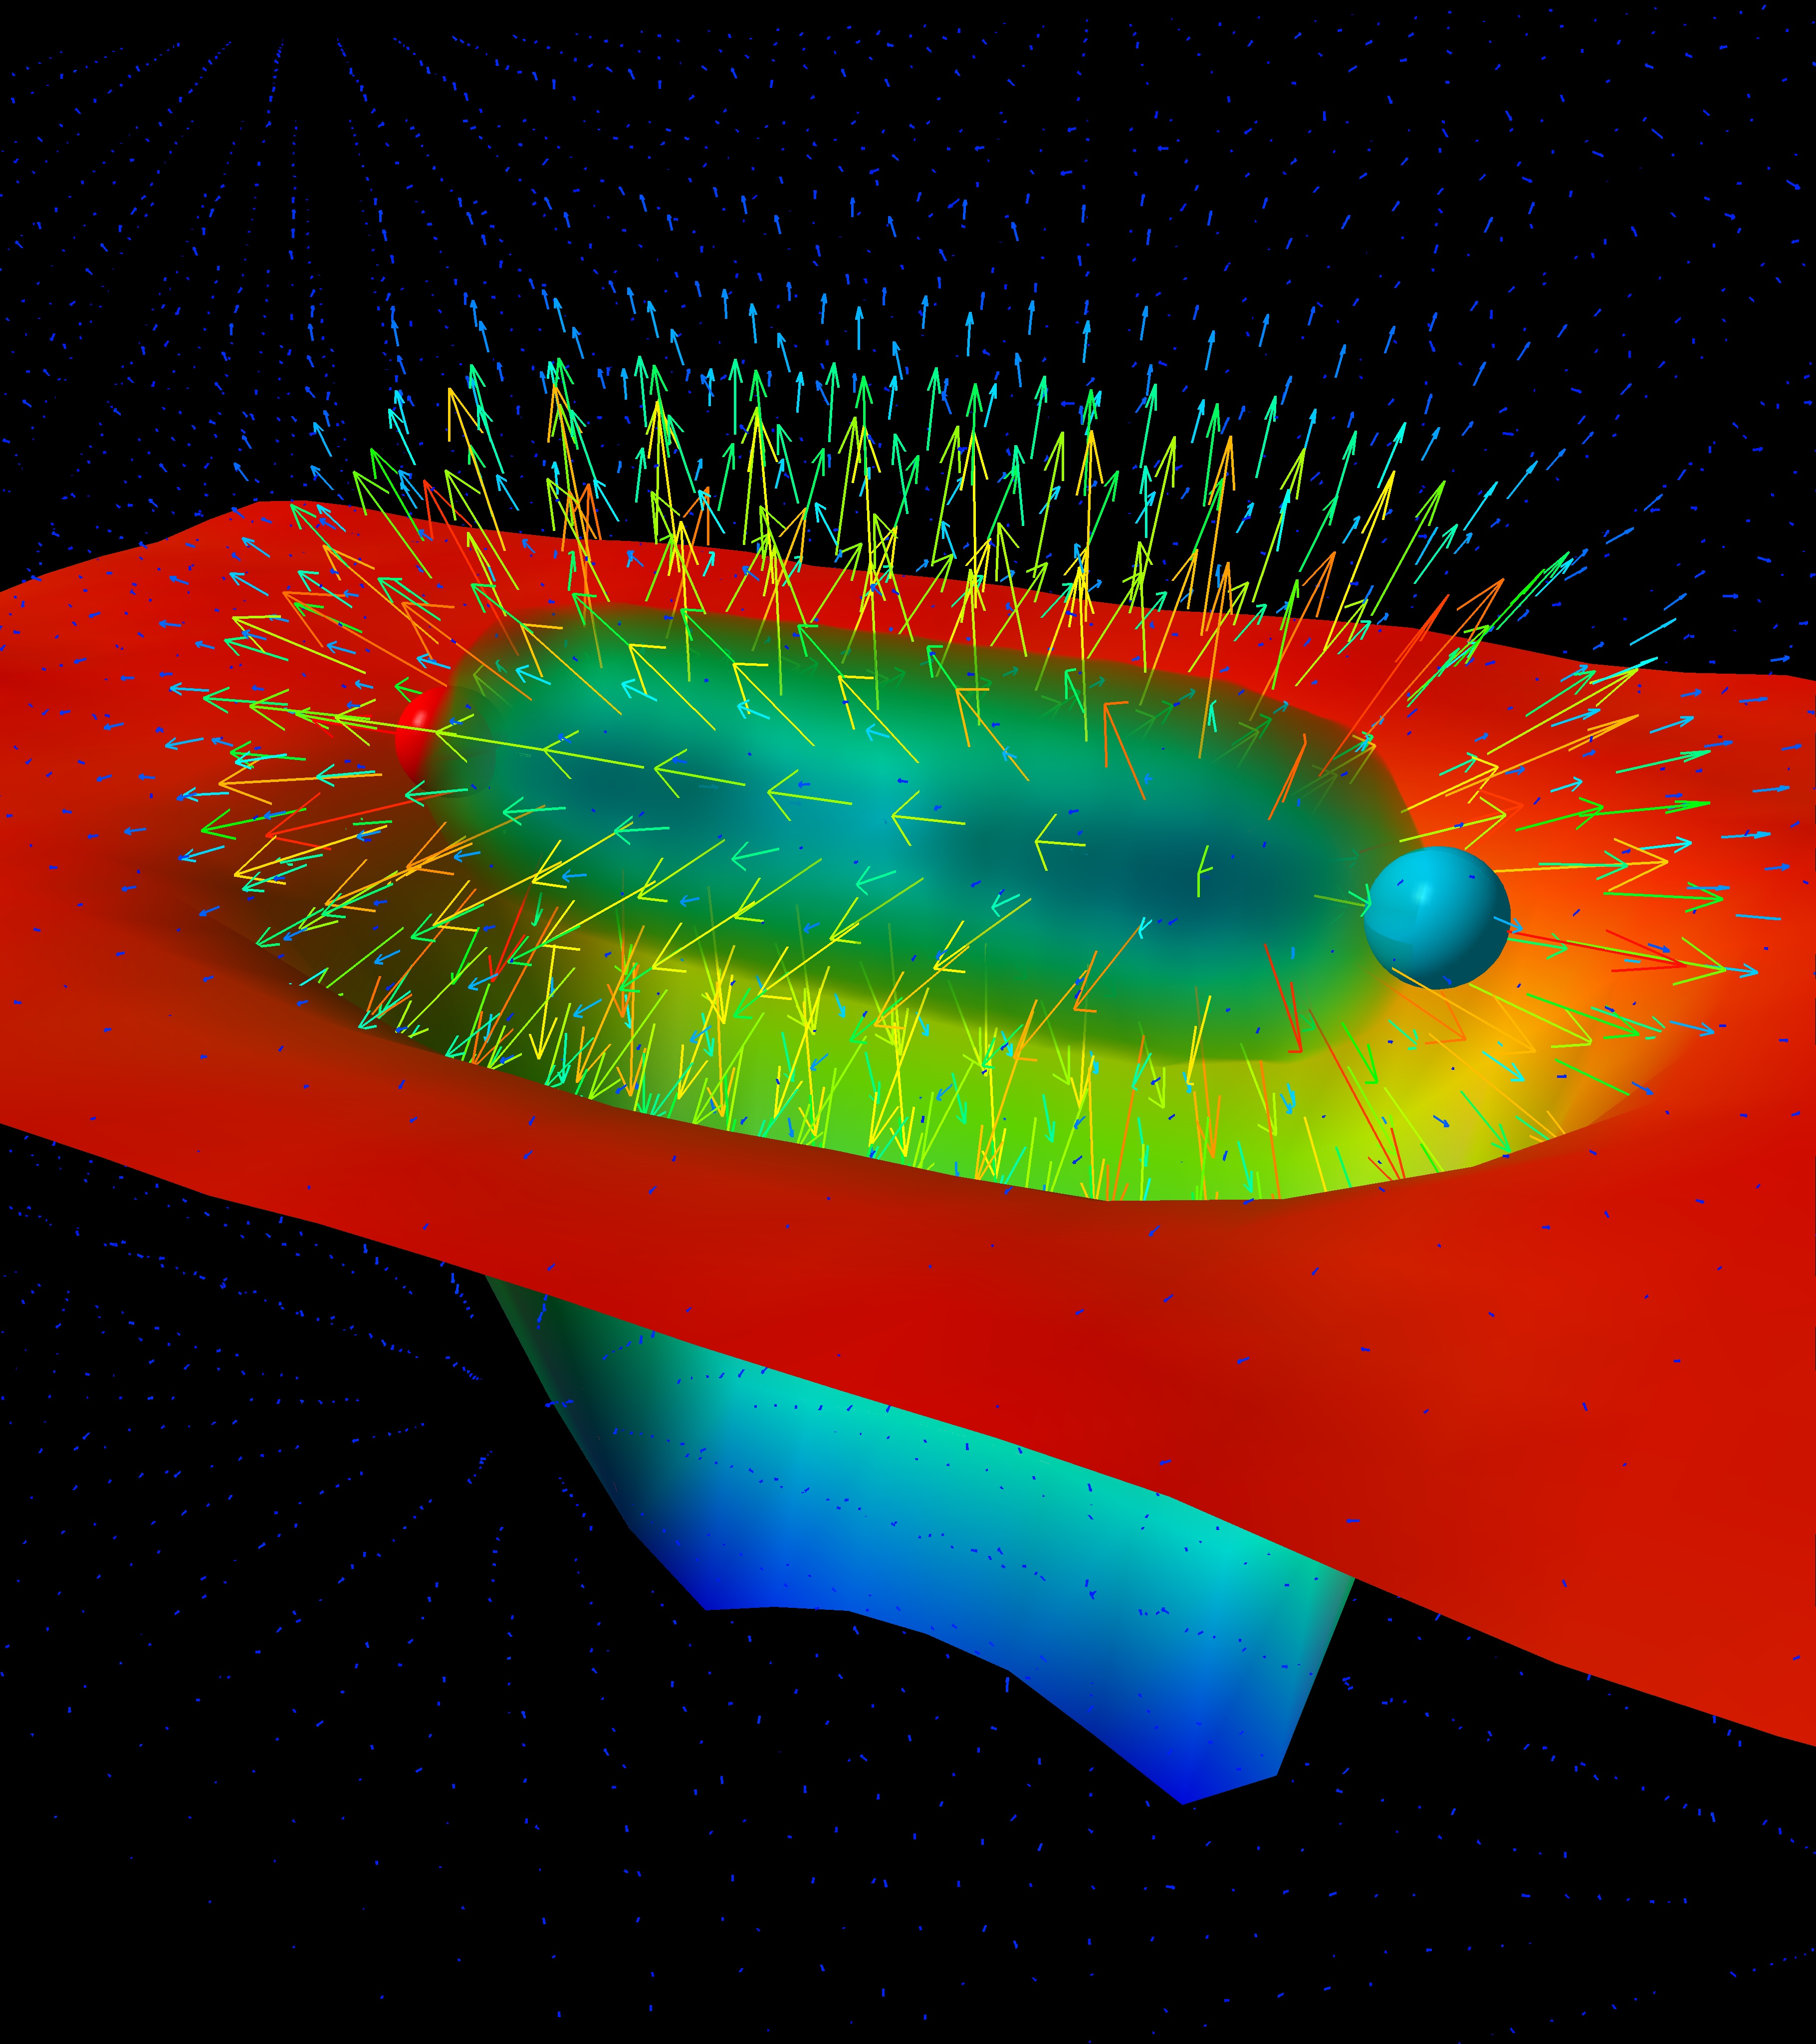
\includegraphics[height=7cm]{figures/01-SM-03-SM/qcd/FluxTube.jpg}
	\hspace{2mm}
	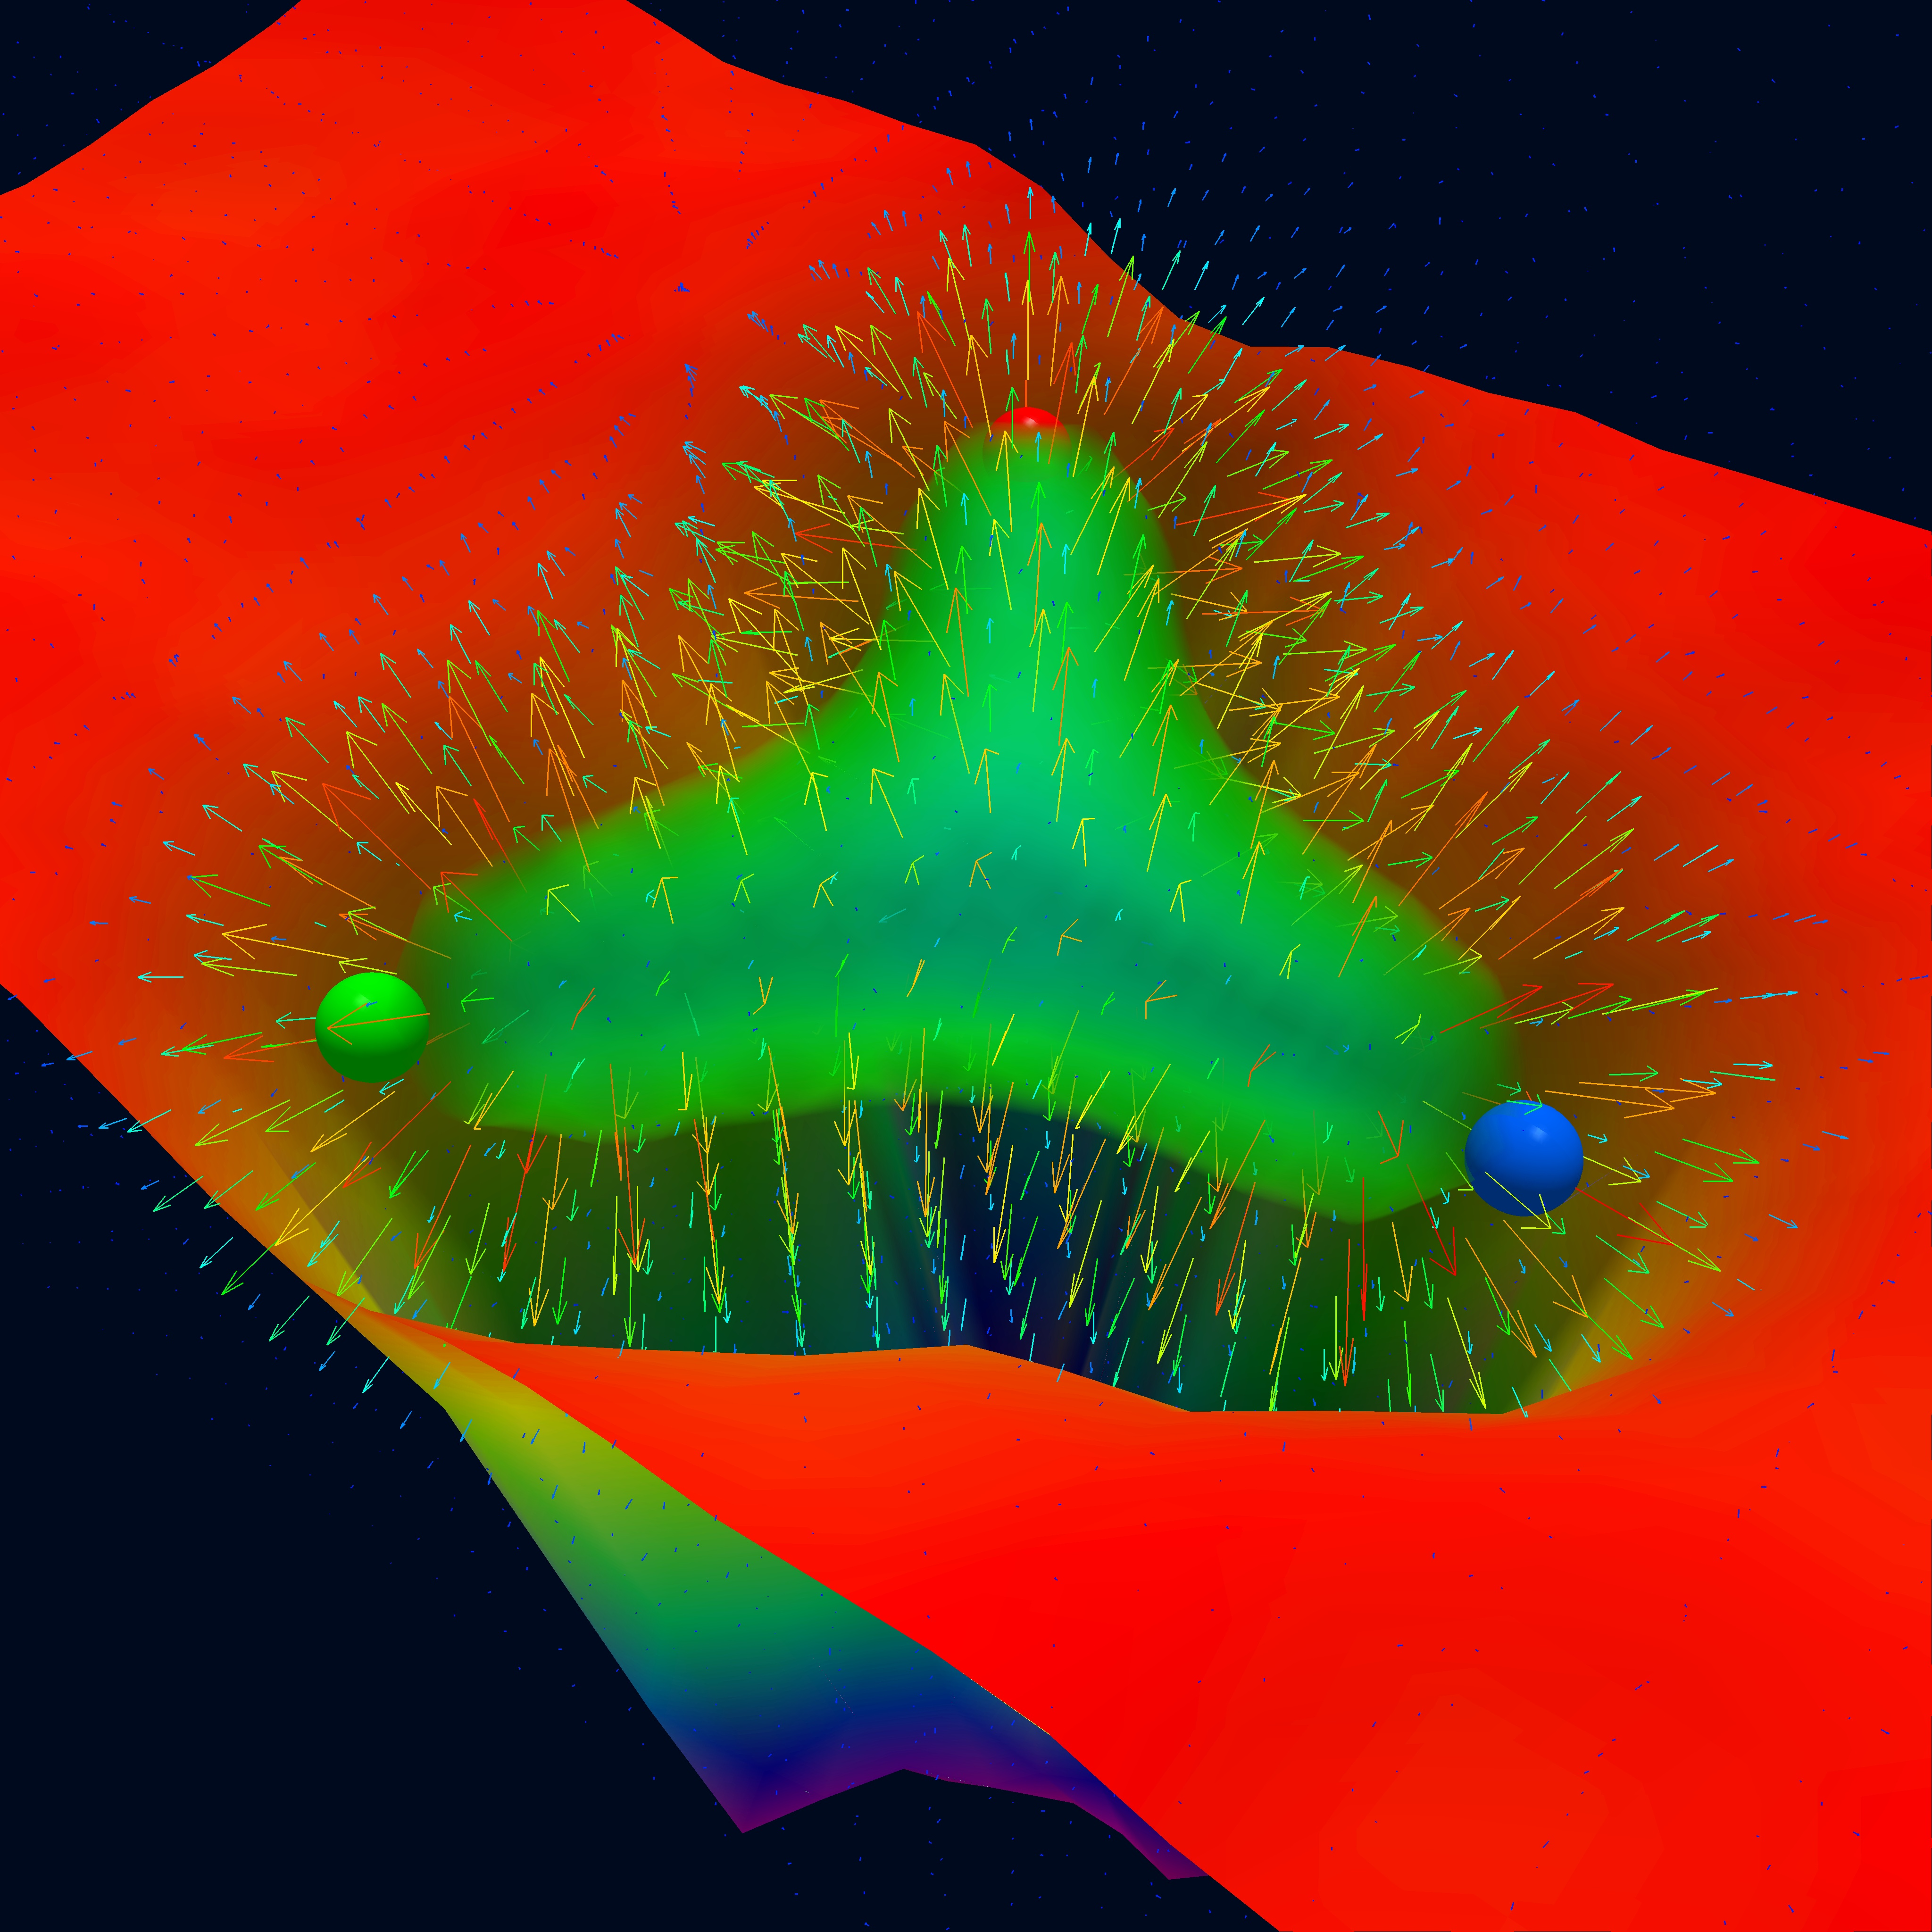
\includegraphics[height=7cm]{figures/01-SM-03-SM/qcd/VacuumRespAction16t32_YshapeCSSMcover.jpg}
	\caption{``Flux tubes'' between a quark and anti-pair inside a meson (left) and three quarks in a proton (right), reproduced from Refs.~\cite{Bissey:2006bz, LeinweberVisualQCD}.}
	\label{fig:01_sm_qcd_fluxtubes}
\end{figure}


\subsection{Quarks and the eightfold way}
\label{sec:01_sm_quarks}

Since their discovery in the 1920s and 30s, the proton and neutron and were believed to be elementary particles along with the electron and photon.
In fact, due to confinement, the first experimental evidence of quarks was not found until the 1960s.
However, already in 1932, the remarkably similar masses of the two nucleons surprised physicists and led Heisenberg, Wigner, and others to hypothesize an underlying \SU[2] symmetry between them (later named \textit{isospin})~\cite{Heisenberg1932, Wigner1937}.
The intrigue only increased in the next decades, during which new cosmic ray, cyclotron, and bubble chamber experiments discovered a veritable ``zoo'' of hadrons, exemplified by a 1964 table of particles in Figure~\ref{fig:01_sm_qcd_particle_zoo}.
While all appeared elementary, several had surprisingly similar properties such as mass and spin, and could also be grouped into invariant subspaces of the isospin group.

\begin{figure}[ht]
	\centering
	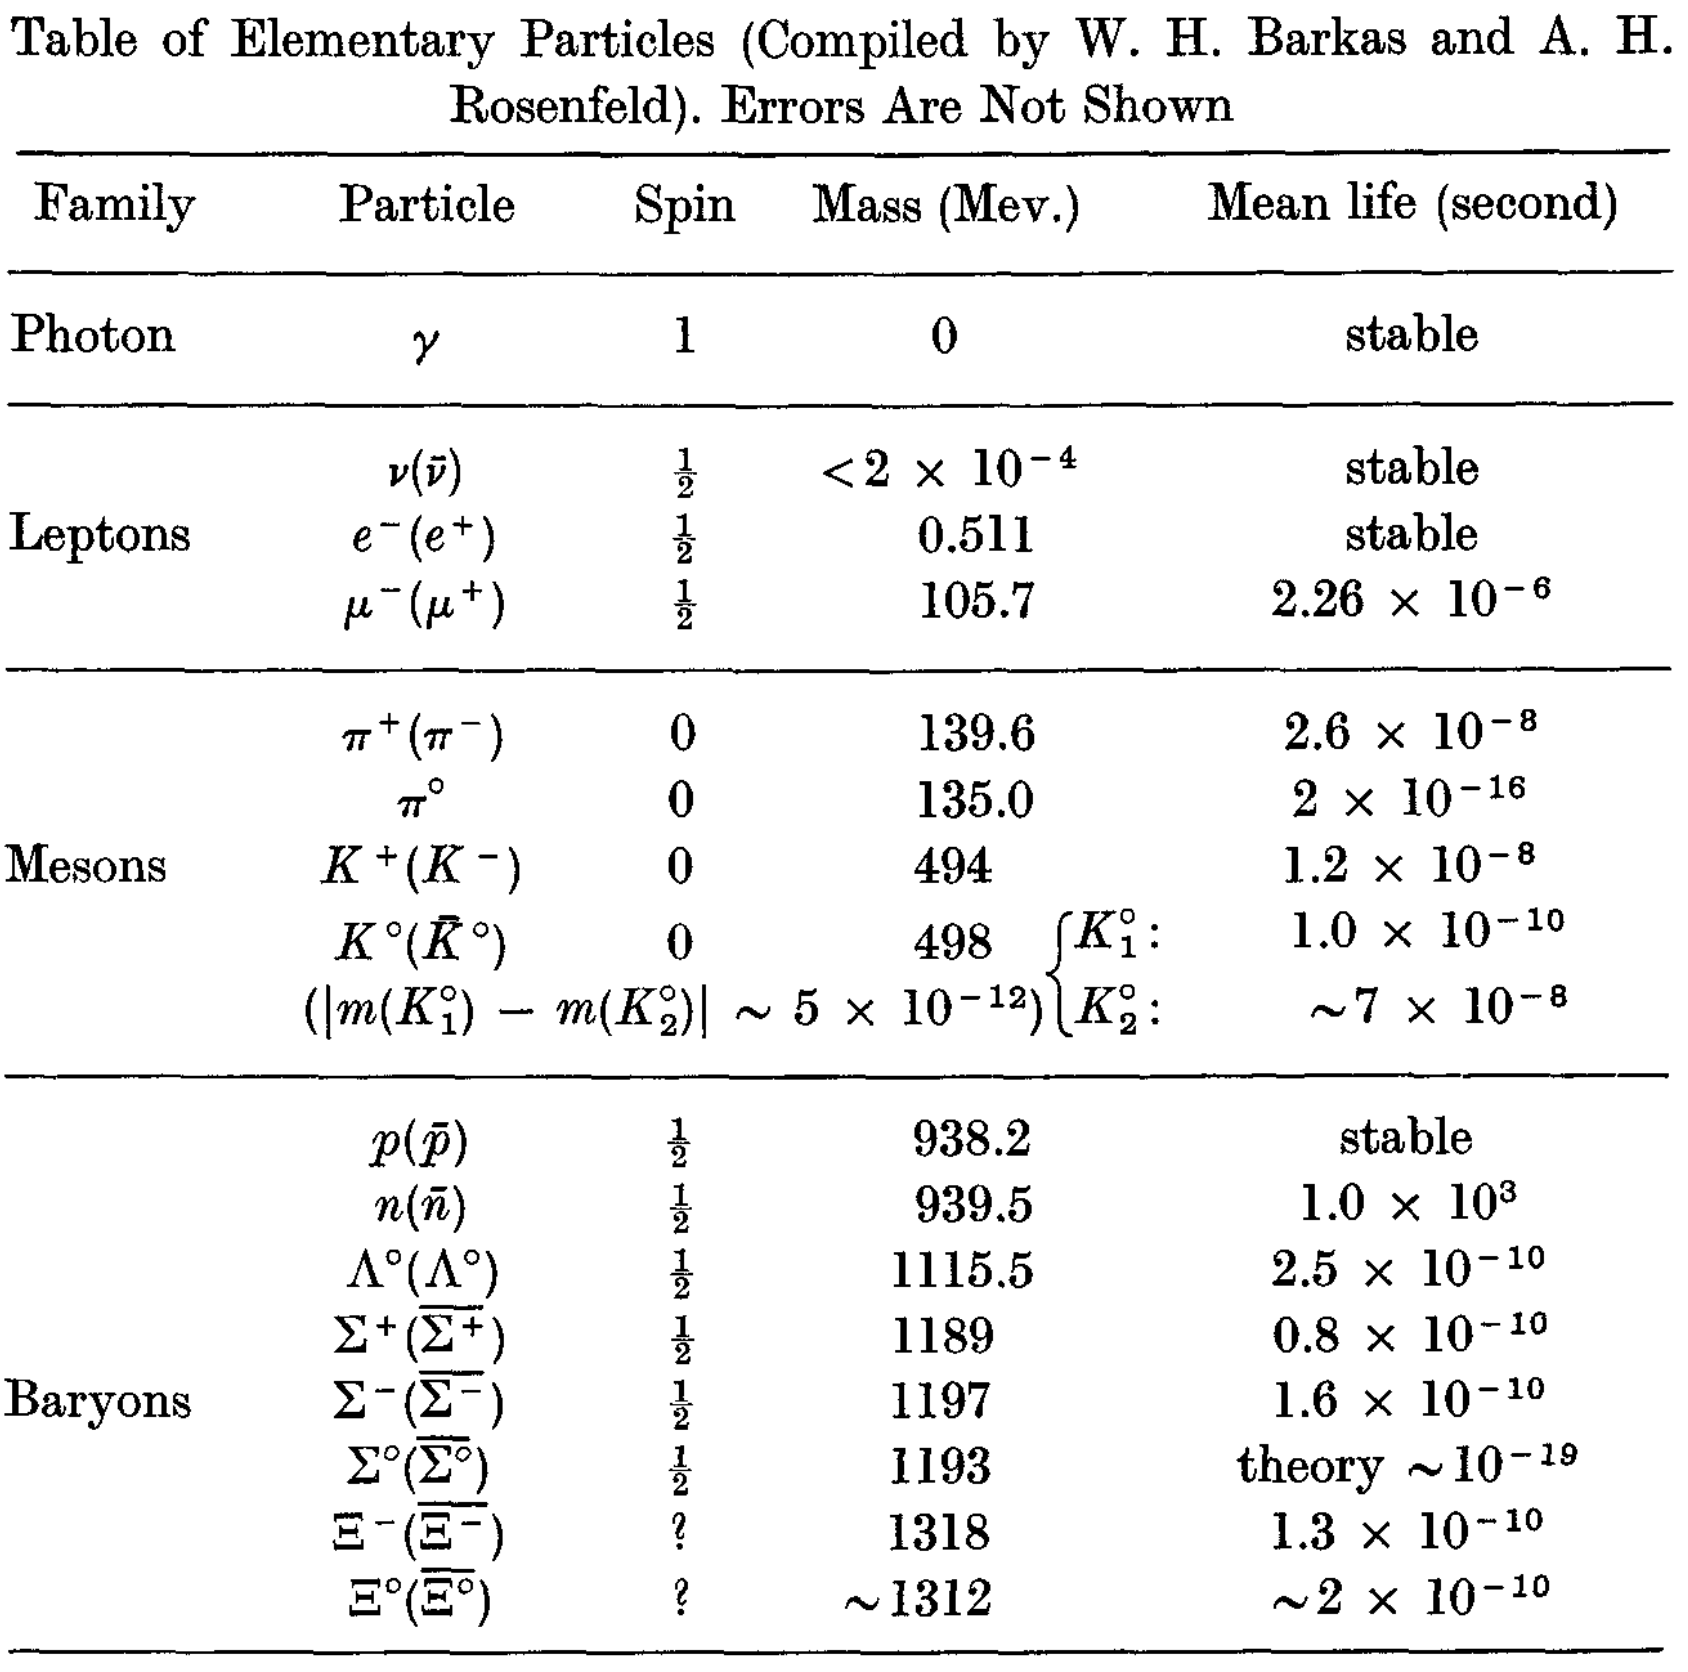
\includegraphics[width=0.8\textwidth]{figures/01-SM-03-SM/qcd/table_elementary_particles_sakurai.png}
	\caption{A table of what were considered to be elementary particles in 1964, reproduced from Ref.~\cite{Sakurai:2015gmk}.}
	\label{fig:01_sm_qcd_particle_zoo}
\end{figure}

In 1961, Murray Gell-Mann and Yuval Ne'eman independently realized that the new hadrons could elegantly fit into representations of a larger symmetry group, \SU[3]~\cite{Gell-Mann:1961omu, Neeman:1961jhl}.
Gell-Mann and George Zweig in 1964 then independently showed that this could be explained physically by hadrons being composed of combinations of three fundamental particles, named the ``up'', ``down'', and ``strange quarks'', with the former two carrying isospin up and down, respectively~\cite{Gell-Mann:1964ewy, Zweig:1964jf}.
% \footnote{Although, interestingly, Gell-Mann himself thought of them as mathematical conveniences than real particles.}
Gell-Mann named this model the ``eightfold way'' (since $\dim (\SU[3]) = 8$) and was awarded the Nobel Prize in 1969 for this work.

Examples of baryons (three-quark hadrons) in the octet and decuplet (dimension 8 and 10, respectively) representations of $\SU[3]$ are shown in Figure~\ref{fig:01_sm_qcd_eightfoldway}, sorted by their isospin along the ``z'' axis ($I_3 = $ \# of up quarks - \# of down quarks) and strangeness ($S = $ \# of strange quarks).
Note that this \SU[3] symmetry is only approximate; it is broken by the different masses of the quarks.
However, their significantly smaller masses compared to $\Lambda_{\mathrm{QCD}}$ mean it remains a useful symmetry for categorizing hadrons.
On the other hand, broader ``symmetries'' such as \SU[4] through \SU[6] including the heavier charm, bottom and top quarks are broken so heavily by their higher masses that they are not helpful for characterizing the heavier hadrons.

\begin{figure}[ht]
	\centering
	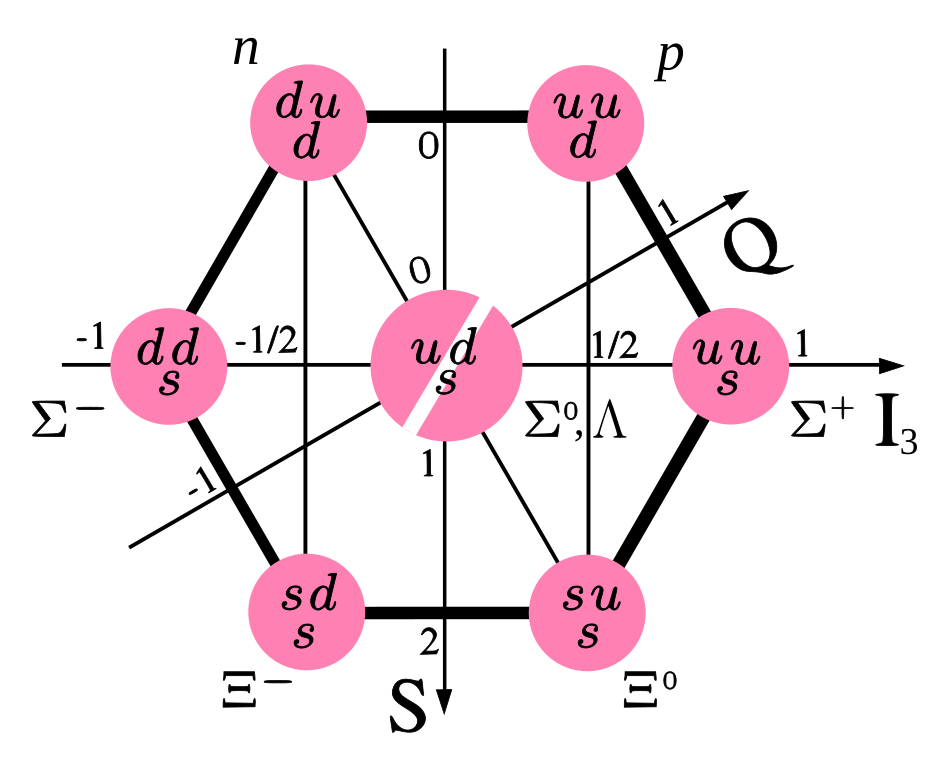
\includegraphics[width=0.45\textwidth]{figures/01-SM-03-SM/qcd/Baryon-octet-small.svg.png}
	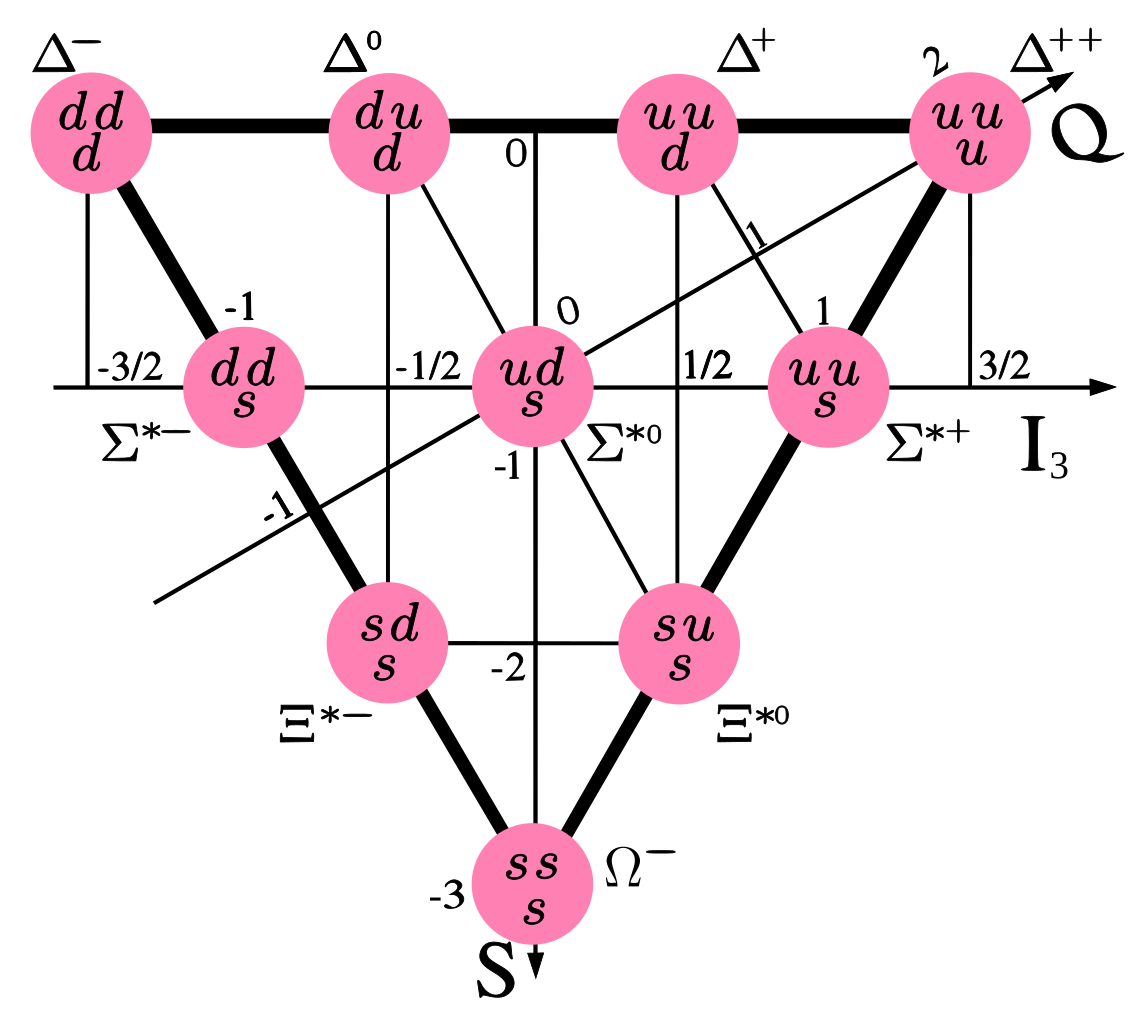
\includegraphics[width=0.45\textwidth]{figures/01-SM-03-SM/qcd/Baryon-decuplet-small.svg.png}
	\caption{Baryons in the octet (left) and decuplet (right) representations of $\SU[3]$, reproduced from Ref.~\cite{enwiki:1243626239}.}
	\label{fig:01_sm_qcd_eightfoldway}
\end{figure}

This fourth ``charm'' quark was notably predicted by Sheldon Glashow, John Iliopoulos, and Luciano Maiani in 1970 to explain the observed suppression of $Z$-boson-mediated flavor-changing neutral currents~\cite{Glashow:1970gm} (and also to match the number of known leptons at the time).
This, and the quark model as a whole, was famously validated by the discovery of a $3.1 \GeV$ charm-anti-charm bound state, named the $J/\psi$ meson, simultaneously by Burton Richter's team at the Stanford Linear Accelerator Center (SLAC) and Samuel Ting's team at Brookhaven National Laboratory in 1974~\cite{SLAC-SP-017:1974ind, E598:1974sol}, both of whom received the Nobel Prize in 1976.

A year before this, Makoto Kobayashi and Toshihide Maskawa had proposed the existence of a \textit{third} generation of quarks to explain the observed CP-violation in weak interactions~\cite{Kobayashi:1973fv}.
This proposal gained more traction after the $J/\psi$ discovery, as well as the discovery of a third-generation lepton, the $\tau$, by Martin Lewis Perl's team in electron-positron collisions at SLAC between 1973 and 1977~\cite{Perl:1975bf}.

In the end, both third generation quarks were discovered at the Fermi National Accelerator Laboratory (Fermilab): first the bottom quark in 1977 by Leon Lederman's team on the E288 experiment~\cite{E288:1977xhf}; and then, much later, the top quark in 1995 by the CDF and DØ experiments at the Tevatron~\cite{CDF:1995wbb, D0:1995jca}.
The bottom quark was discovered indirectly, as with the charm quark, through the observation of a bottom quark-antiquark bound state called bottomium, or the $\Upsilon$ meson, in proton-nucleon collisions.

The top quark, on the other hand, is highly unique because of its high $173 \GeV$ mass, and it decays too quickly to form bound states.
Hence, it is the only quark to have been observed ``directly'', through its decays to a $W$ boson and a bottom quark.
It is the heaviest known elementary particle, which is why its discovery required the 1\TeV center-of-mass energy proton-antiproton collisions of the Tevatron.
The unique nature of the heavy quarks leads to a rich phenomenology at high energy colliders such as the LHC, particularly in the context of the \textit{jets} they form (Section~\ref{sec:01_sm_qcd_jets}).

% and hence could be discovered directly through its decays to a $W$ boson and a bottom quark in proton-antiproton collisions.
% Indeed, because of its high mass, it is unable to form bound states, decaying too quickly, and is the only quark that can decay directly to other particles.
% in proton-nucleon collisions which produced a bottom-antibottom bound state called bottomium, or the $\Upsilon$ meson~\cite{E288:1977xhf}

% in proton-antiproton collisions

% The top quark turns out to be highly unique due to its high $173 \GeV$ mass.
% It is the heaviest known elementary particle, which is why its discovery required the 1\TeV center-of-mass energy collisions of the Tevatron.
% It cannot form hadronic bound states due to its short lifetime, and is the only quark that can directly decay to other particles (primarily to a $W$ boson and a bottom quark).
% The unique nature of the heavy quarks leads to a rich phenomenology at high energy colliders such as the LHC, particularly in the context of the \textit{jets} they form, as will be discussed in \TODO{??}.

\subsection{The parton model}
\label{sec:01_sm_qcd_quarks_parton}

Some physicists, including Gell-Mann himself, initially believed quarks not to be real particles but simply mathematical conveniences to describe hadrons.
It was only through \textit{deep inelastic scattering} (DIS) experiments in the 1960s and 70s at SLAC --- in which high energy electrons were shot at protons (in the form of hydrogen) to probe their inner structure --- that it was confirmed that protons are indeed not point-like particles.

To explain this behavior, Richard Feynman and others proposed the \textit{parton model} of the proton (and other hadrons).
In this, protons are composed of point-like particles called \textit{partons} that are what actually interact with the electrons in DIS, as illustrated in Figure~\ref{fig:01_sm_qcd_dis}.
Though initially partons were abstract entities, we now identify them as the quarks and gluons of QCD.
At the energies required for DIS (and modern hadron colliders), the ``partonic'' cross-section of electron-parton scattering (or parton-parton scattering) ($\hat\sigma$) can be calculated using standard perturbation theory and Feynman diagrams.

To then derive the total ``hadronic'' electron-proton cross-section, we must integrate over all possible electron-parton interactions, weighted by the probability of finding a parton carrying a fraction $x$ of the proton's momentum at an energy scale $Q^2$.
This is described by the \textit{parton distribution functions} (PDFs) $f_i(x, Q^2)$, where $i$ represents the type of parton.
PDFs cannot be calculated perturbatively and must be determined from experimental data.
Examples for the proton at $Q^2 = 10 \GeV$ are shown in Figure~\ref{fig:01_sm_qcd_pdfs}; observe that the up and down quarks --- called the \textit{valence} or ``real'' quarks --- dominate at high $x$, while at lower $x$ there are gluons as well as other \textit{sea} (i.e., virtual) quarks.

The overall hadronic cross-section for DIS is thus:
\begin{equation}
	\label{eq:01_sm_qcd_sigma_ep}
	\sigma_{eh} = \sum_{i} \int_0^1 \dd x f_i(x, Q^2) \hat\sigma_{ei}(Q^2, \mu_r),
\end{equation}
where $\mu_r$ is the scale used for renormalization when calculating the partonic cross-sections.
The separation of the perturbative and nonperturbative parts of the cross-section is called \textit{factorization}, and the fact that this is possible is proved in the \textit{factorization theorem}~\cite{Collins:1989gx}.

As also illustrated in Figure~\ref{fig:01_sm_qcd_dis}, high energy hadron-hadron collisions such as those at the LHC involve a similar, but more complicated, interaction.
The corresponding cross-section involves integrating over two partons' momenta (one each from the two colliding hadrons):
\begin{equation}
	\label{eq:01_sm_qcd_sigma_pp}
	\sigma_{hh} = \sum_{i, j} \int_0^1 \dd x_1 \dd x_2 f_i(x_1, Q^2) f_j(x_2, Q^2) \hat\sigma_{ij}(Q^2, \mu_r).
\end{equation}
% where $\mu_r$ is the scale used for renormalization when calculating the partonic cross-sections.
This is known as the ``master formula'' for cross-sections at the LHC.\footnote{See lectures by Torsten Pfoh~\cite{Pfoh:2012Lectures} and Joey Huston~\cite{Huston:2018Lectures} for useful pedagogical discussions.}
PDFs are generally measured via DIS at electron-proton colliders, and are then crucial inputs to the above equation for hadron colliders.
There is also hope of deriving these through lattice QCD simulations.

\begin{figure}
	\centering
	\adjustbox{valign=m}{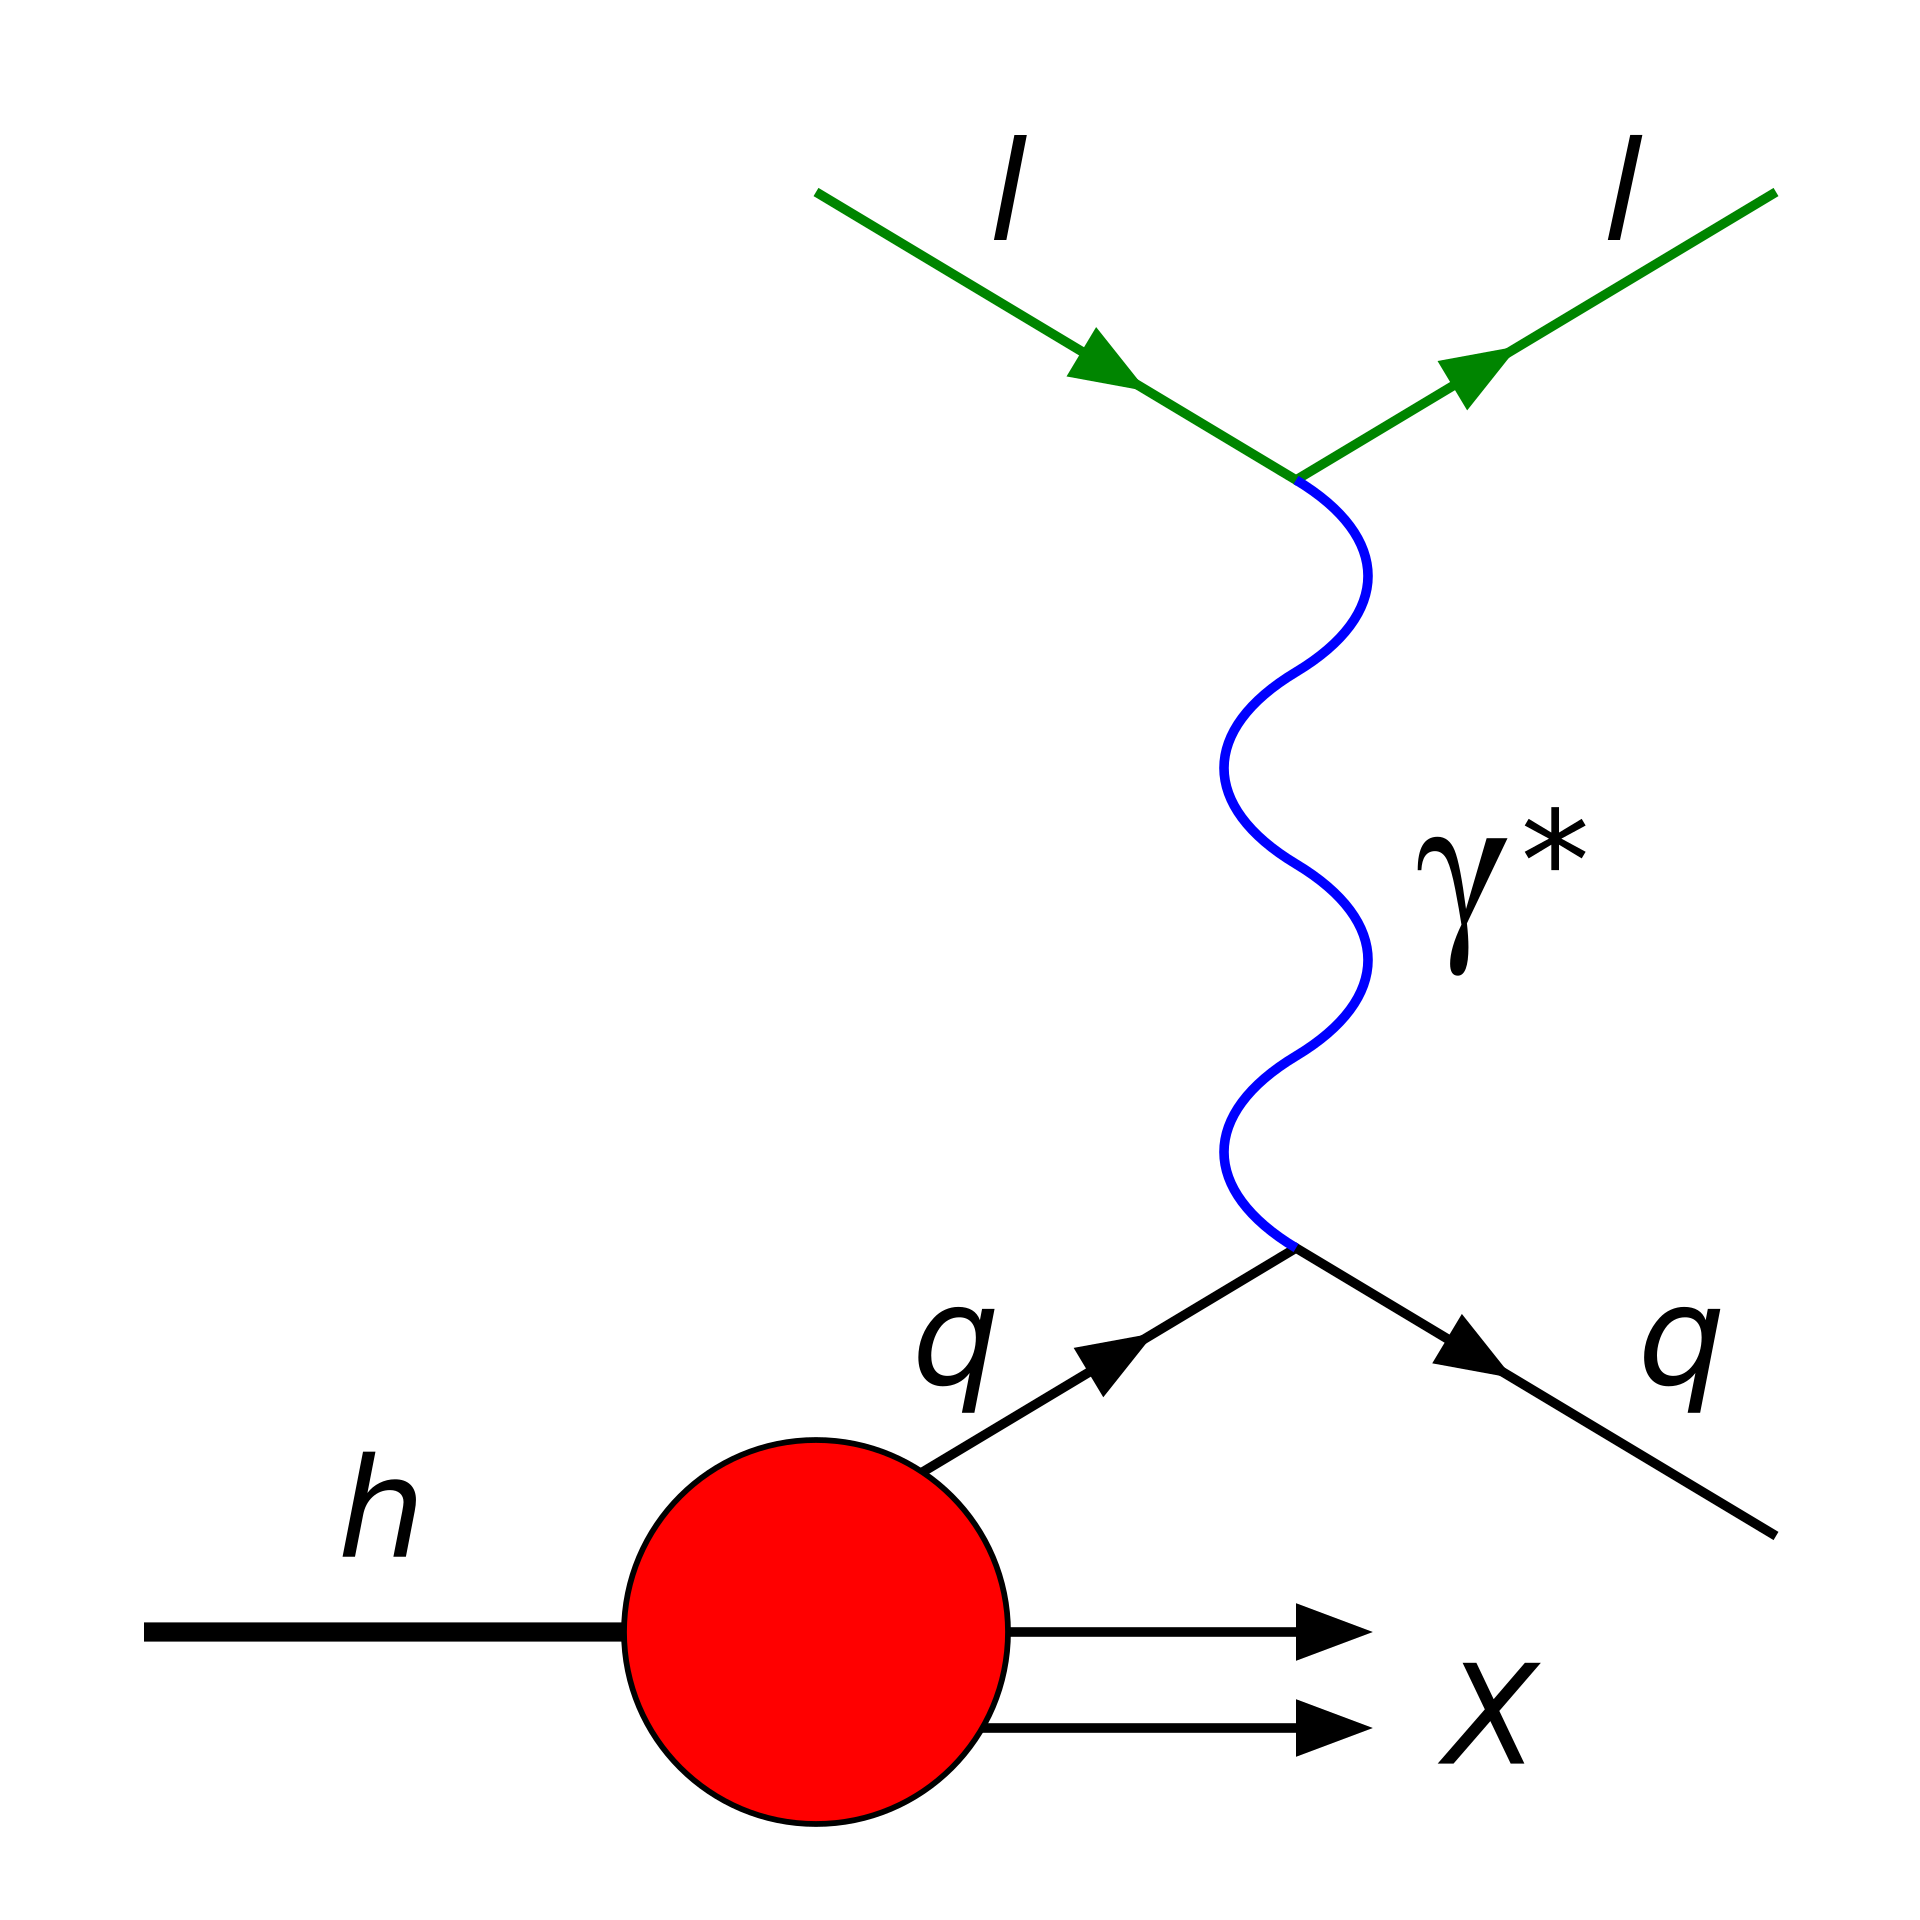
\includegraphics[width=0.3\textwidth]{figures/01-SM-03-SM/qcd/DIS.svg.png}}
	\hspace{1cm}
	\adjustbox{valign=m}{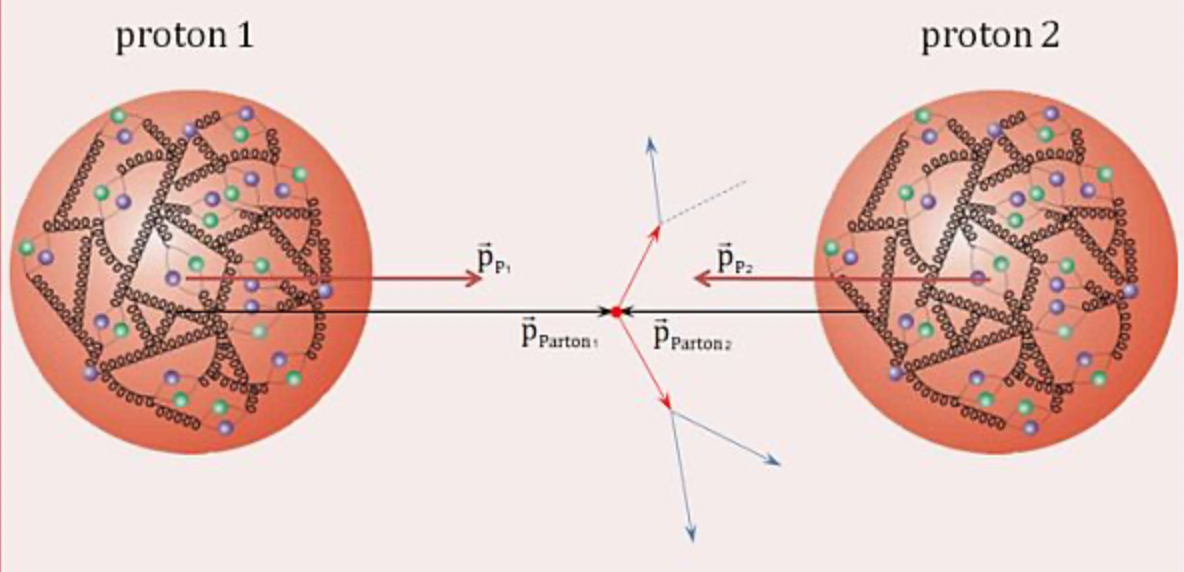
\includegraphics[width=0.45\textwidth]{figures/01-SM-03-SM/qcd/proton-proton.png}}
	\caption{Feynman diagram for deep inelastic scattering, reproduced from Ref.~\cite{enwiki:1240848406} (left) and an illustrative example of proton-proton collisions reproduced from Ref.~\cite{ATLAS:2024protoncollisions} (right).}
	\label{fig:01_sm_qcd_dis}
\end{figure}

\begin{figure}
	\centering
	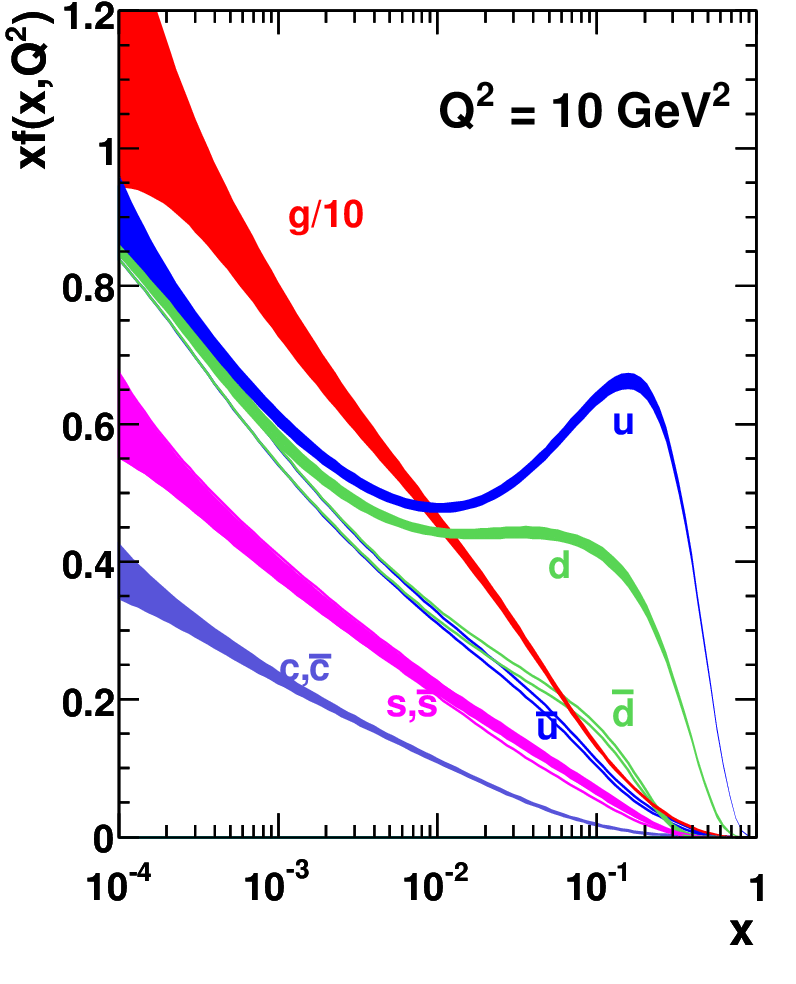
\includegraphics[width=0.5\textwidth]{figures/01-SM-03-SM/qcd/The-MSTW-2008-proton-PDFs.png}
	\caption{PDFs for the proton at $Q^2 = 10 \GeV$, reproduced from Ref.~\cite{Krasny2010}.}
	\label{fig:01_sm_qcd_pdfs}
\end{figure}

\subsubsection{The partonic cross section}

The partonic cross-section $\hat\sigma(Q^2, \mu_r)$ is an important theoretical input for measurements at high energy colliders.
The dependence on $\mu_r$ is perhaps surprising; however, it represents the fact that $\hat\sigma$ is calculated perturbatively: the $\mu_r$ dependence only appears in the highest order term of the expansion.
Indeed, this scale dependence would disappear at infinite order in perturbation theory.
While it may seem a nuisance, in fact, it provides a convenient handle to estimate the \textit{uncertainties} on our theoretical predictions by simply varying $\mu_r$ and $\mu_f$.\footnote{See Ref.~\cite{Salam:2010zt} 4.1 for further discussion.}

One important feature to keep in mind regarding the perturbative calculations for hadron colliders is that the leading order (LO) predictions are often a factor of $\gtrsim 2$ off the higher order next-to-LO (NLO) and next-to-NLO (NNLO) calculations.
This is exemplified in the predictions for \PZ boson production at the LHC, shown in Figure~\ref{fig:01_sm_qcd_qcd_nlo}.
The reason for this, despite $\alpha_s$ being reasonably small ($\approx 0.1$) at the scale for this process $m_Z \simeq 90\GeV$, is simply that the $\mathcal O(\alpha_s)$ corrections have large coefficients~\cite{Salam:2010zt}.
This is why measurements at the LHC relying on LO simulations often multiply the cross-section with an NLO / LO ``K-factor''.

Practically, matrix elements are first calculated as a function of the input and output ``hard particle'' momenta, after which event generator programs such as \MADGRAPH~\cite{Alwall:2014hca} use Monte Carlo (MC) methods to sample events appropriately from the overall phase space.
NLO and NNLO calculations are more complicated and often involve weighting events negatively to represent subtractions at higher orders~\cite{Danziger:2021xvr}.

\begin{figure}[ht]
	\centering
	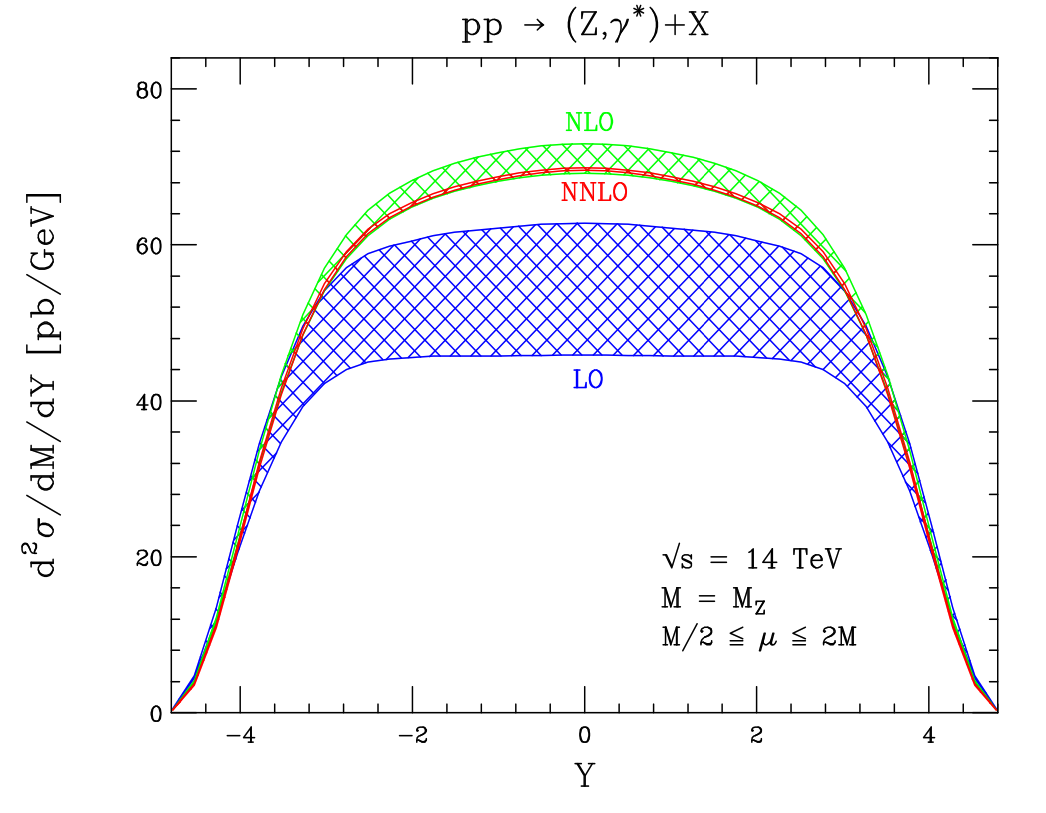
\includegraphics[width=0.7\textwidth]{figures/01-SM-03-SM/qcd/Zxs.png}
	\caption{LO, NLO, and NNLO predictions and uncertainties for $pp$ to Z boson production, differential in rapidity $Y$ at the LHC, reproduced from Ref.~\cite{Anastasiou:2003ds}.}
	\label{fig:01_sm_qcd_qcd_nlo}
\end{figure}


\subsubsection{Parton evolution}

Each parton has a certain probability of radiating another quark or gluon, with a fraction of the original parton's momentum, $z$.
These are called parton splitting functions, $P_{ij}(z)$, depicted in Figure~\ref{fig:01_sm_qcd_splitting}, and can be calculated perturbatively in QCD (see e.g. Ref.~\cite{Salam:2010zt}).
They are then further convolved with PDFs to derive their evolution with the energy scale:
\begin{equation}
	\label{eq:01_sm_qcd_pdf_evolution}
	\frac{\dd f_i(x, Q^2)}{\dd Q^2} = \frac{1}{Q^2} \sum_{j} \int_x^1 \frac{\dd z}{z} f_j(\cnicefrac{x}{z}, Q^2) P_{ji}(z).
\end{equation}

Equations~\ref{eq:01_sm_qcd_pdf_evolution} are called the Dokshitzer-Gribov-Lipatov-Altarelli-Parisi (DGLAP) evolution equations, after five physicists who developed them in the 1970s, and are analogous to the renormalization group flows of coupling constants.
The dependence of the PDFs on the energy scale has been confirmed in DIS experiments, which are then also used to fit the parameters of the PDFs, as shown in Figure~\ref{fig:01_sm_qcd_dglap}.

\begin{figure}[ht]
	\centering
	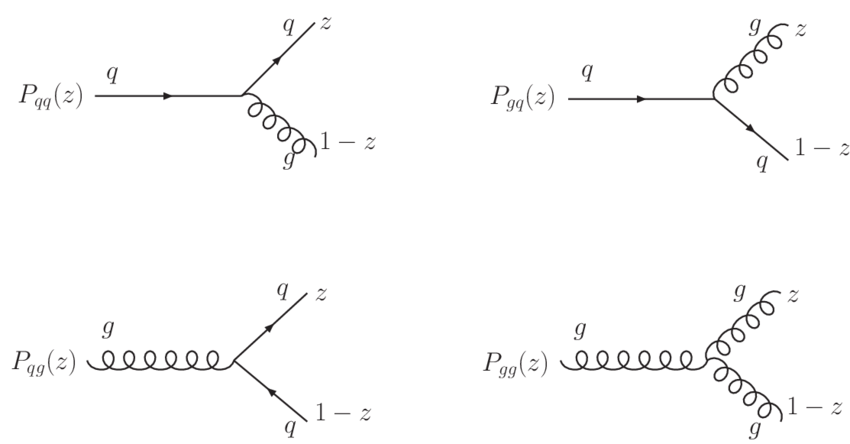
\includegraphics[width=0.9\textwidth]{figures/01-SM-03-SM/qcd/The-splitting-functions.png}
	\caption{The splitting functions for quarks and gluons, reproduced from Ref.~\cite{Kollar:2007TopQuark}.}
	\label{fig:01_sm_qcd_splitting}
\end{figure}

\begin{figure}[ht!]
	\centering
	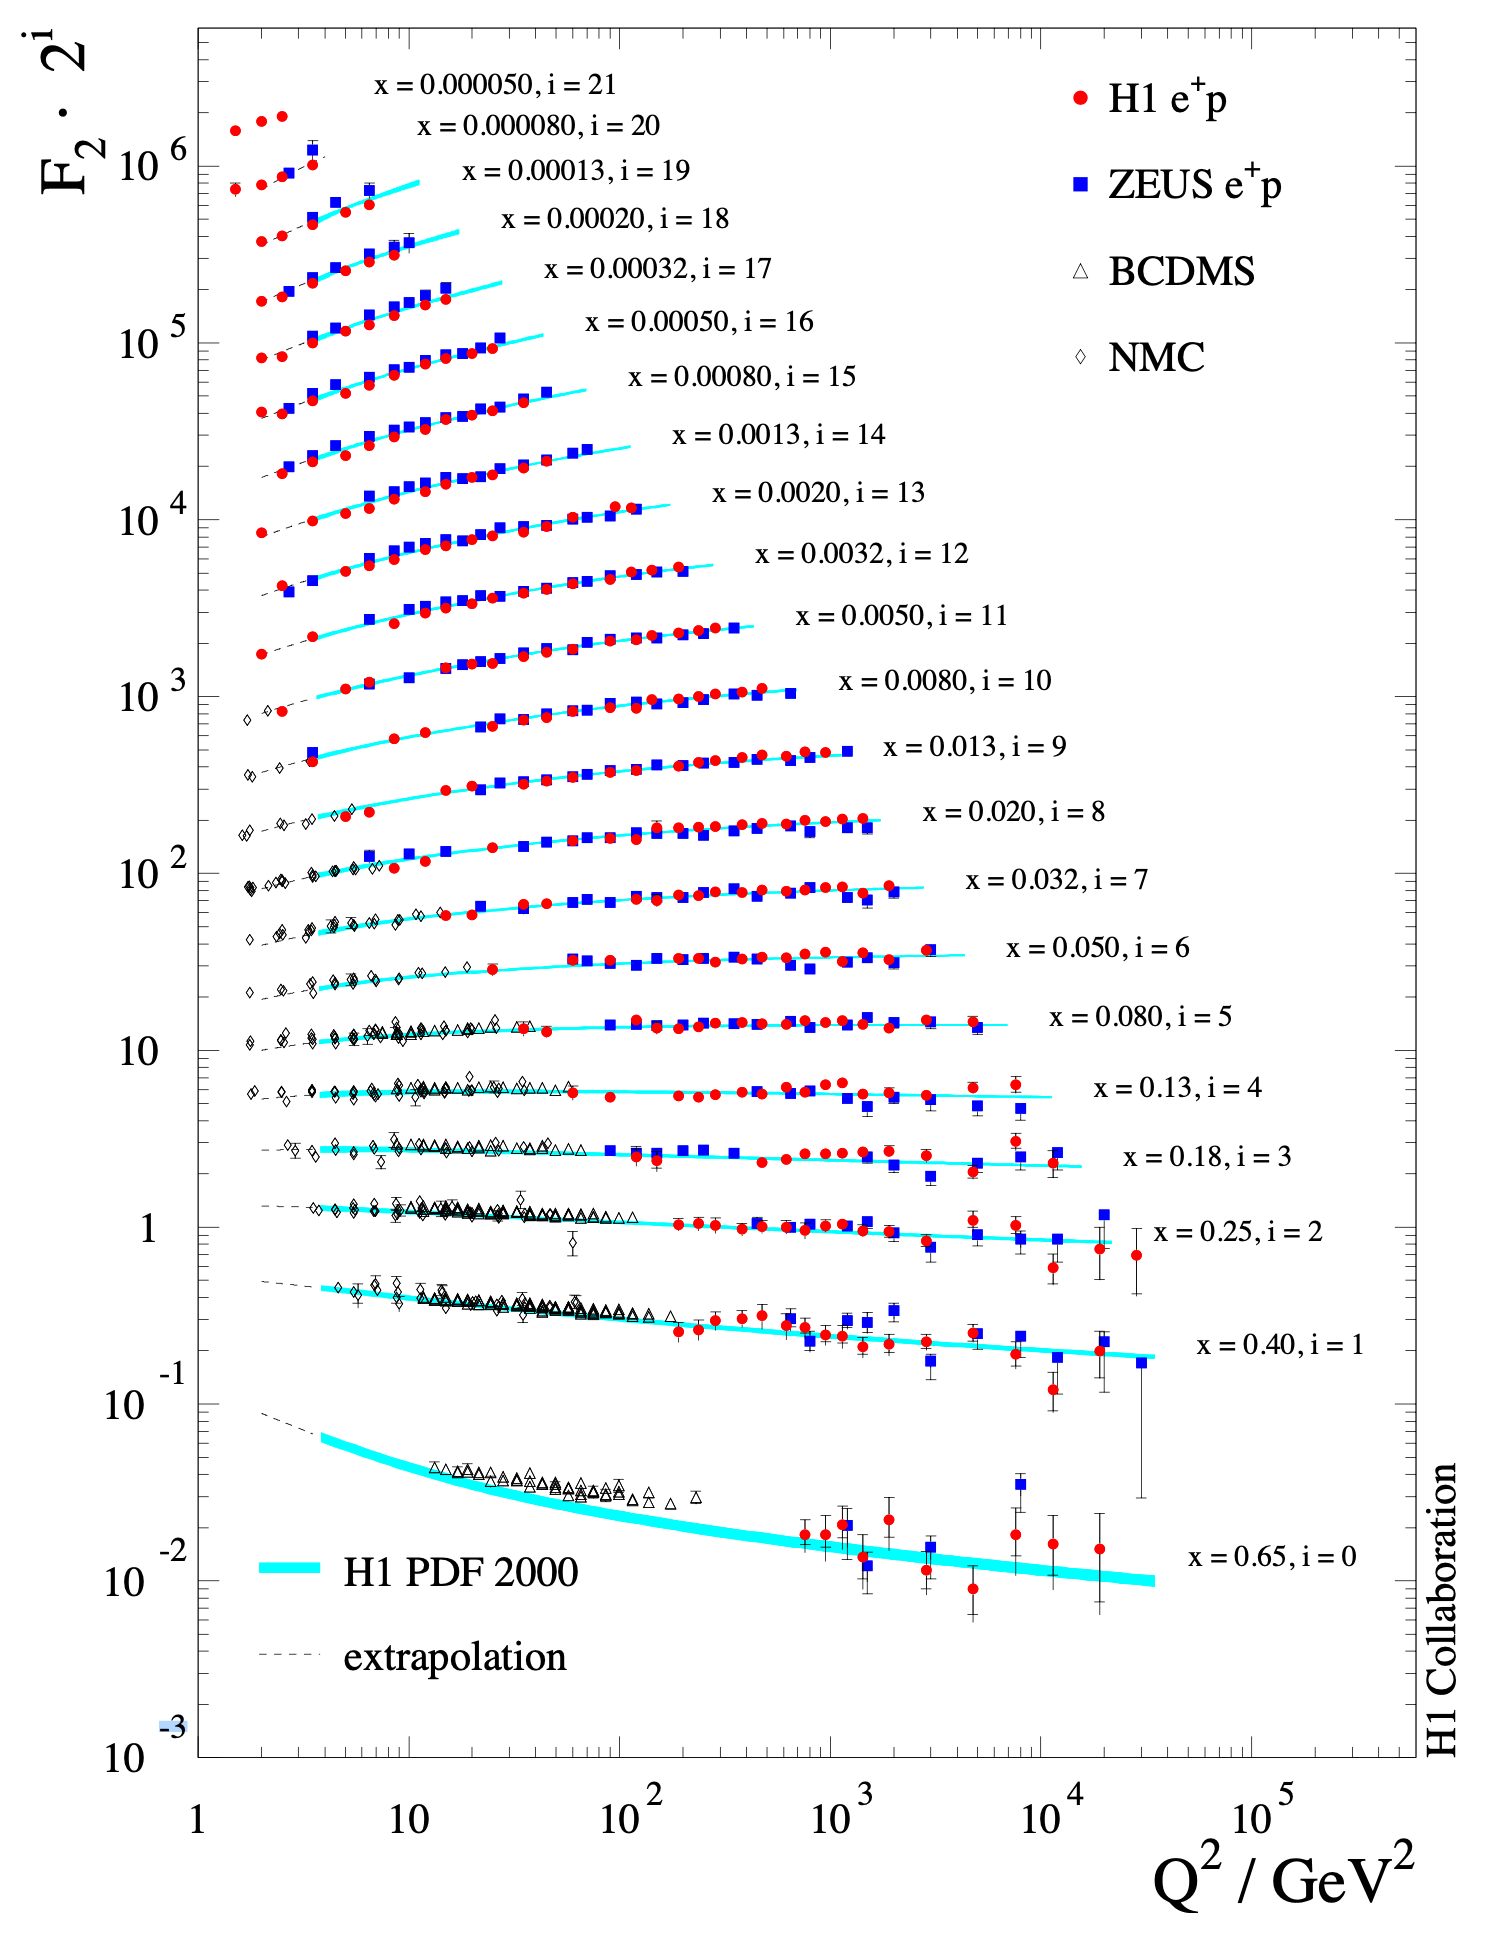
\includegraphics[width=0.75\textwidth]{figures/01-SM-03-SM/qcd/HERA_DIS.png}
	\caption{PDF measurements at different energy scales $Q^2$ and momentum fraction $x$ by the H1 collaboration in DIS experiments, reproduced from Ref.~\cite{Glazov:2007zz}.}
	\label{fig:01_sm_qcd_dglap}
\end{figure}


\subsection{Jets}
\label{sec:01_sm_qcd_jets}

As one may infer from the DGLAP equations (Eq.~\ref{eq:01_sm_qcd_pdf_evolution}), when high energy partons are produced at a collider, they will probabilistically radiate further and further partons --- called \textit{parton showering} --- until they approach the confinement scale and start forming bound hadrons --- called \textit{hadronization}.
For sufficiently high energy initial partons, the resulting hadrons will appear as a collimated spray of particles in the detector, called a \textit{jet} (Figures~\ref{fig:01_sm_qcd_jet_cartoon} and~\ref{fig:01_sm_qcd_jet_event}).

Since quarks and gluons are never observed in isolation, their production can only be inferred by understanding the jets they form.
Moreover, at a hadron collider, the high-energy hadrons continuously radiate partons \textit{before} and \textit{after} the collision as well, with the resulting jets referred to as \textit{initial} and \textit{final state radiation} (ISR and FSR), respectively.
Such jets are by far the most prevalent outputs of collisions at the LHC and, hence, represent a significant background in many measurements and searches, particularly those searching for hadronic final states.

\begin{figure}[ht]
	\centering
	\captionsetup{justification=centering}
	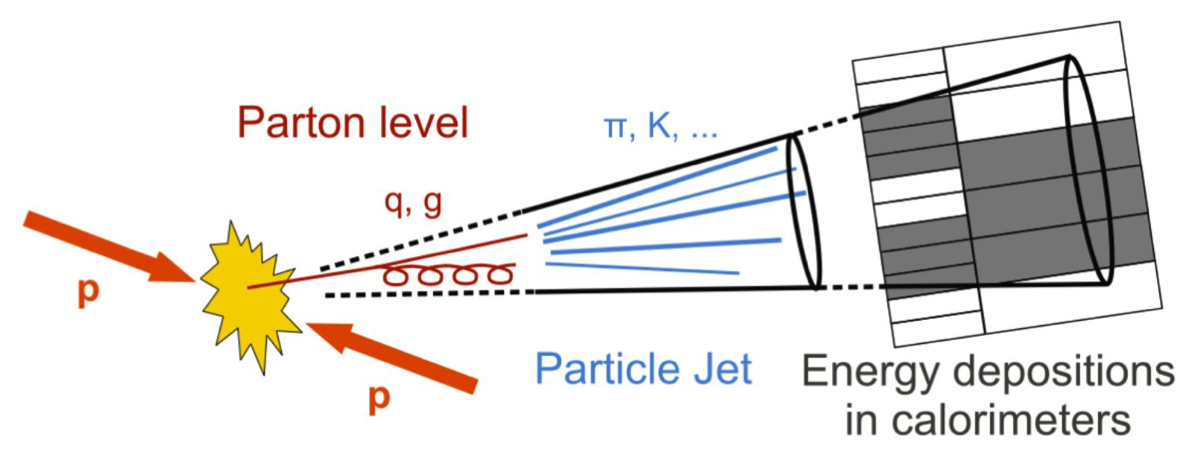
\includegraphics[width=\textwidth]{figures/01-SM-03-SM/qcd/jet_cartoon.png}
	\caption{A cartoon of a jet, reproduced from Ref.~\cite{Kirschenmann:2014vga}.}
	\label{fig:01_sm_qcd_jet_cartoon}
\end{figure}

\begin{figure}[ht]
	\centering
	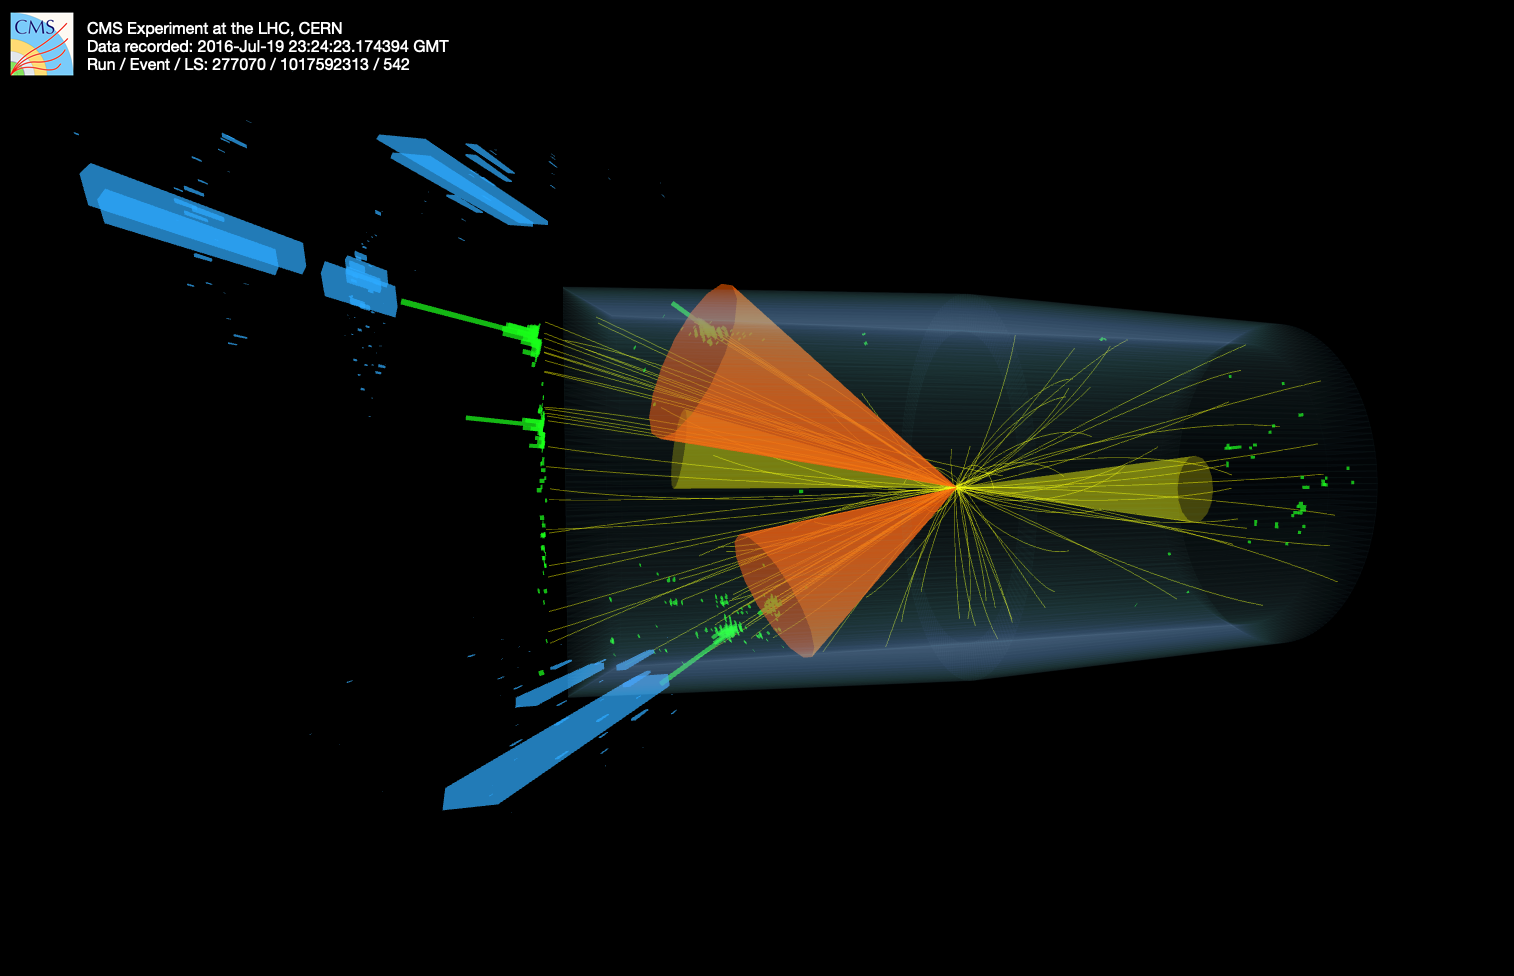
\includegraphics[width=\textwidth]{figures/01-SM-03-SM/qcd/bbww_event.png}
	\caption{An example of real jets in an event collected by CMS and identified in the search described in Chapter~\ref{sec:05_hh}~\cite{Bauerdick:2011zz, CMS:2024les}.
	An interactive version of this event display is available at \url{https://cms3d.web.cern.ch/HIG-23-012/.}}
	\label{fig:01_sm_qcd_jet_event}
\end{figure}


\subsubsection{Parton showering}

Jets can be understood and modeled by factorizing the dynamics.
As above, the parton scattering cross section (referred to as the \textit{hard process} and calculated perturbatively) is separated from the PDFs (measured from data) and their evolution (DGLAP equations).
This evolution is what produces the showering, and is modeled by numerically iterating through $Q^2$ (or, equivalently, through time) and randomly emitting new partons according to the splitting functions via MC sampling.

There are several subtleties involved in this process which numerical parton shower generators, such as \PYTHIA~\cite{Sjostrand:2014zea}, \HERWIG~\cite{Corcella:2000bw}, and \SHERPA~\cite{Sherpa:2019gpd} must account for.
First, the probability of gluon emission diverges in the soft --- i.e., low gluon energy --- and collinear --- small gluon angle with the parent parton --- limits.
Physically, this can be interpreted as the limit of our experimental resolution: at a certain point we cannot resolve two close-by or detect arbitrarily soft particles.

These are known as the \textit{infrared} and \textit{collinear} (IRC) divergences, respectively, and are typically regulated by introducing cut-off energies and angles for emissions (below which we can reasonably argue that perturbation theory is anyway invalid).
These divergences also mean that when analyzing jets in experimental data, care must be taken in defining observables to be \textit{IRC-safe}, meaning that jet clustering algorithms and physical properties derived therein should not be sensitive to arbitrarily soft or collinear emissions.

Another issue is that a naive combination of the hard matrix element and subsequent parton shower calculations may lead to double-counting of emissions, as illustrated in Figure~\ref{fig:01_sm_qcd_doublecounting}.
This necessitates a careful ``matching procedure'', such as the most common MLM scheme~\cite{Alwall:2007fs}, which defines cut-off energy and angular scales to separate the matrix element and parton shower phase spaces.
Other considerations include preserving unitarity, color coherence and color flow, and differences between ISR and FSR (see e.g. Refs.~\cite{Hoche:2014rga, Hoche:2018Lecture}).

\begin{figure}[ht]
	\centering
	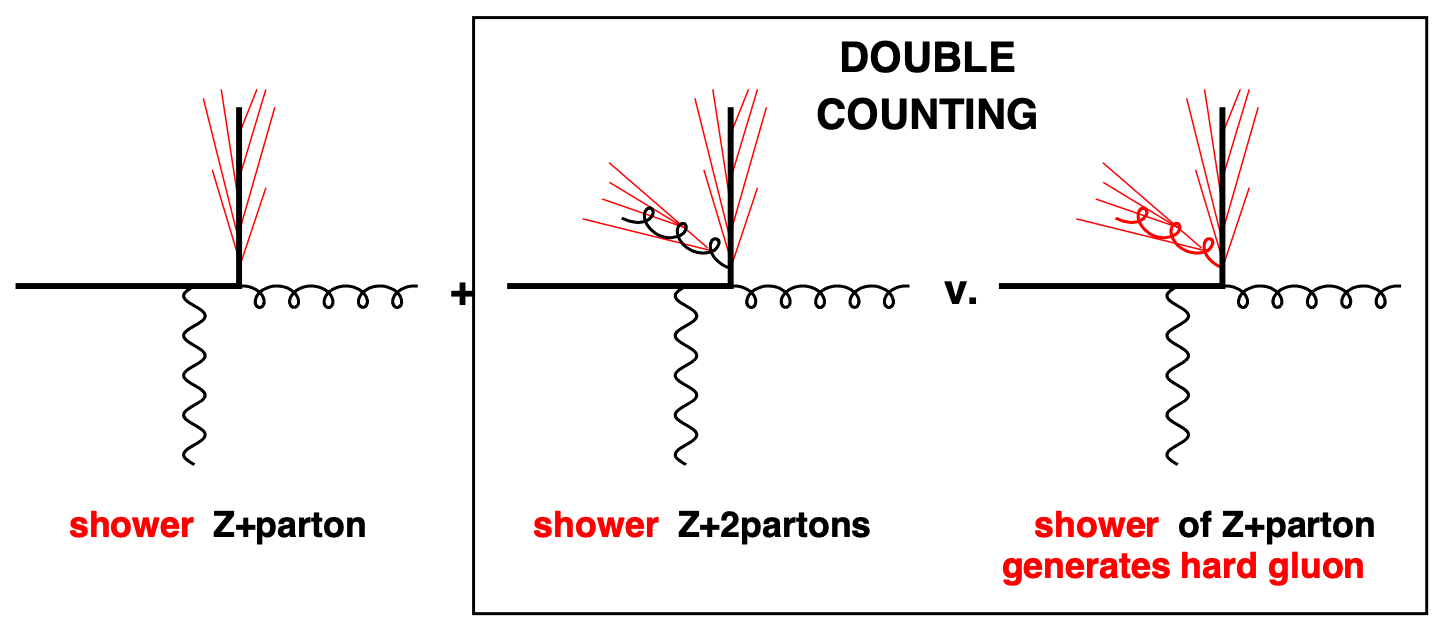
\includegraphics[width=0.8\textwidth]{figures/01-SM-03-SM/qcd/double_counting.png}
	\caption{An illustration of double-counting when combining matrix element predictions (in black) with parton showering algorithms (in red) for $Z+$parton and $Z+$2-parton events, reproduced from Ref.~\cite{Salam:2010zt}.}
	\label{fig:01_sm_qcd_doublecounting}
\end{figure}


\subsubsection{Hadronization}

The final element of the factorized process is hadronization, once the parton shower approaches the confinement scale.
This is a completely nonperturbative process and, hence, like PDFs, we must rely on numerical simulations and experimental measurements.

Lattice QCD simulations, such as those shown in Figure~\ref{fig:01_sm_qcd_fluxtubes}, indicate that in the low energy limit, the effective potential between quarks increases linearly with distance, resembling string tension:
\begin{equation}
	\label{eq:01_sm_qcd_string}
	V(r) = \sigma r,
\end{equation}
where $\sigma$ is the string tension coefficient.
In fact, this analogy can be extended further: above a certain energy, the string appears to ``snap'', in the sense that it becomes possible and energetically more favorable to produce a quark-antiquark pair.

This analogy the basis of the \textit{Lund string model} of hadronization~\cite{Andersson:1983ia}, illustrated in Figure~\ref{fig:01_sm_qcd_lundstring}.
The strong force between the final state partons is modeled as a series of strings stretched between them that probabilistically break into new partons.
Other models are based on clustering partons into color-neutral combinations~\cite{Corcella:2000bw}.

\begin{figure}[ht]
	\centering
	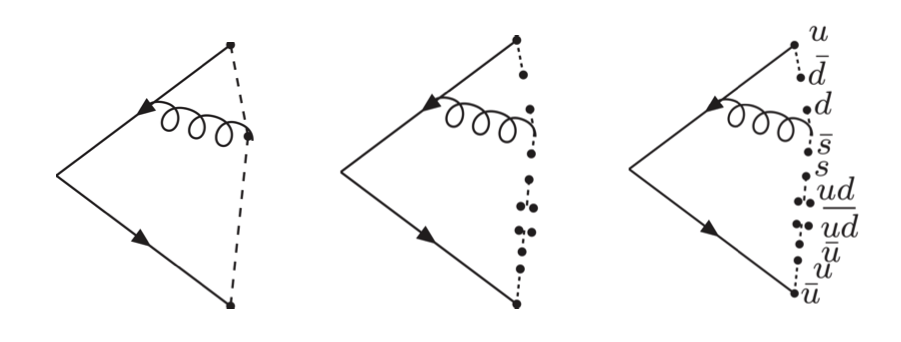
\includegraphics[width=0.6\textwidth]{figures/01-SM-03-SM/qcd/Lund_string.png}
	\caption{An illustration of the Lund string model of hadronization, reproduced from Ref.~\cite{Prestel:2018Lecture}.}
	\label{fig:01_sm_qcd_lundstring}
\end{figure}


% \subsubsection{Defining jets}

% As discussed above, it is important to define jets in an IRC-safe way.

%  - kT class of algorithms, anti-kT is most common \\

% \subsubsection{Identifying jets}

%  - jetnet cartoon \\
%  - quarks vs gluons \\
%  - ``heavy jets'', b jets \\
%  - jet substructure for boosted tops, Higgs \\

% \subsection{Chiral symmetry breaking}


\section{Electroweak interactions}
\label{sec:01_sm_ew}

The weak interaction is the last of the three fundamental forces we discuss in the SM.
Apart from its relatively weak coupling constant (Table~\ref{tab:01_sm_coupling_constants}), it is unique in several ways: (1) it couples only to left-chiral fermions, thereby violating parity ($P$) and charge conjugation ($C$); (2) it is the only force with massive gauge bosons, resulting in short-range interactions; and (3) it is the only force that ``sees'' and can change the flavors of the fermions.
Hence, it is responsible for radioactive decays and the instability of all hadrons and leptons bar the proton and electron.
Its couplings to the different flavors also lead to $CP$-violation, as we discuss in Section~\ref{sec:01_sm_ew_flavor}.

\subsection{Weak interactions}
\label{sec:01_sm_ew_weak}

The first theory of weak interactions was Enrico Fermi's 1933 theory of beta decay~\cite{Fermi:1934hr}: the decay of the neutron to a proton, $n \to p + e^- + \bar\nu_e$, through a four-fermion interaction (Figure~\ref{fig:01_sm_ew_fermi}, left).
Fermi was inspired by Dirac's nascent theory of QED, and using similar perturbative techniques, his theory proved successful in describing weak decays.
The same principle was also applied to other weak decays, such as muon decay (Figure~\ref{fig:01_sm_ew_fermi}, right) and pion decay.

As it turned out, the four-fermion interaction is of mass dimension $6$ and not renormalizable (see Chapter~\ref{sec:01_qft_interactions}), leading to the scattering cross-section diverging at high energies.
This is, of course, because these interactions are in fact mediated by the massive weak $W^\pm$ and $Z$ gauge bosons, which become relevant around their mass scale of $\mathcal O(100\GeV)$.
We now understand the Fermi theory as an effective field theory (EFT) valid for energies much lower than $100 \GeV$, wherein the $W$ and $Z$ boson DoFs can be integrated out and nonrenormalizable interactions are allowed --- they are just suppressed by factors of $(\cnicefrac{1}{M_W})^2$.
This suppression is why the weak interaction is so weak, with a coupling constant of $\approx \mathcal O(10^{-6})$ at the mass scale of the proton.

\begin{figure}[ht]
	\centering
	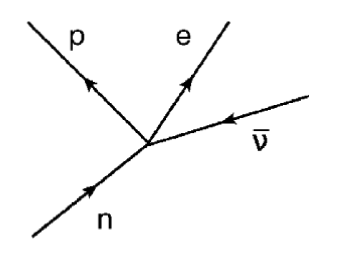
\includegraphics[width=0.25\textwidth]{figures/01-SM-03-SM/ew/beta_decay.png}
	\hspace{1cm}
	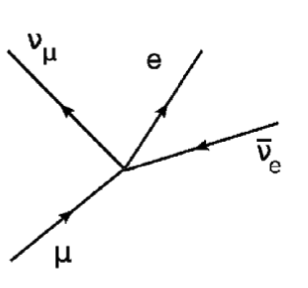
\includegraphics[width=0.2\textwidth]{figures/01-SM-03-SM/ew/muon_decay.png}
	\caption{Feynman diagrams for beta decay (left) and muon decay (right) in Fermi's theory.}
	\label{fig:01_sm_ew_fermi}
\end{figure}

% The discovery of the non-renormalizability of Fermi's theory in the 1950s led to disenchantment with QFT~\cite{WeinbergHistoryQFT}.
% with the advent of Yang-Mills theory, it was proposed that 

The weak interaction is described by an \SU[2] Yang-Mills theory, and is sometimes referred to as quantum flavordynamics (QFD) because of its deep connection to flavor, as we will discuss.
However, ``vanilla'' Yang-Mills theories cannot accommodate massive gauge bosons; hence, it was only after the development of the ABEGHHK (Higgs) mechanism in the 1960s that this description gained traction.
Specifically, Sheldon Glashow, Abdus Salam, Steven Weinberg and others showed that the spontaneous breaking of an \SU[2] $\times$ \UU[1] symmetry to \UU[1] could not only yield massive weak gauge bosons, but also naturally incorporate QED with a massless photon~\cite{Glashow:1959wxa, Salam:1968rm, Weinberg:1967tq}.

This combined \textit{electroweak} theory has been experimentally confirmed in many stages: 
first with the discovery of \textit{neutral currents} involving neutrinos with the Gargamelle bubble chamber at CERN in 1973~\cite{GargamelleNeutrino:1973jyy}, the first evidence for the $Z$ boson (the only neutral boson that couples to neutrinos); 
then with the direct discovery of the $W$ and $Z$ bosons at the Super Proton Synchrotron (SPS) in 1983~\cite{UA1:1983crd, UA1:1983mne, UA2:1983tsx, UA2:1983mlz}, as well as precision measurements of electroweak parameters such as the $W$ and $Z$ masses with the Large Electron-Positron Collider (LEP) in the 1990s; 
and finally with the discovery of the Higgs boson at the LHC in 2012~\cite{CMS:2012qbp, ATLAS:2012yve}, a particle predicted by the ABEGHHK mechanism, and the ongoing measurements of its properties.


\subsection{Before electroweak symmetry breaking}

Electroweak interactions are associated with the $\SU[2]_L \times \UU[1]_Y$ gauge symmetry, which is ``spontaneously broken'' to $\UU[1]_{\text{EM}}$ through the ABEGHHK mechanism during electroweak symmetry breaking (EWSB).\footnote{As discussed in Chapter~\ref{sec:01_qft_higgs}, technically, the gauge symmetry cannot be broken --- what breaks is the associated global symmetry.}
We label the three gauge bosons of $\SU[2]_L$ as $W^1, W^2, W^3$ and of $\UU[1]_Y$ as $B$, with coupling constants $g$ and $g'$, respectively.

The fermions in the SM can be categorized by their representations, or charges, under the three gauge symmetries before EWSB, as in Table~\ref{tab:01_sm_ew_fermions}.
The bold numbers indicate the dimension of the representation under the respective symmetry group, while the regular numbers are the charges under the $\UU[1]_Y$ group --- referred to as their \textit{hypercharge}, $Y$.

\begin{table}[ht]
	\renewcommand{\arraystretch}{1.5}
	\centering
	\caption{The representations and charges of fermionic and scalar fields in the SM under the $\UU[1]_Y$, $\SU[2]_L$, and $\SU[3]_C$ gauge symmetries. 
	The right-handed neutrino is included here for completeness but has not been experimentally confirmed.}
	\begin{tabular}{c|ccc}
		\toprule
		 & $\UU[1]_Y$ & $\SU[2]_L$ & $\SU[3]_C$ \\
		\midrule
		$Q_L$ & $+ \cnicefrac{1}{6}$ & $\mathbf{2}$ & $\mathbf{3}$ \\
		$L_L$ & $- \cnicefrac{1}{2}$ & $\mathbf{2}$ & $\mathbf{1}$ \\
		$u_R$ & $+ \cnicefrac{2}{3}$ & $\mathbf{1}$ & $\mathbf{3}$ \\
		$d_R$ & $- \cnicefrac{1}{3}$ & $\mathbf{1}$ & $\mathbf{3}$ \\
		$e_R$ & $-1$ & $\mathbf{1}$ & $\mathbf{1}$ \\
		$\nu_R$? & $0$ & $\mathbf{1}$ & $\mathbf{1}$ \\
		$H$ & $+ \cnicefrac{1}{2}$ & $\mathbf{2}$ & $\mathbf{1}$ \\
		\bottomrule
	\end{tabular}
	\label{tab:01_sm_ew_fermions}
\end{table}

The weak interactions specifically are associated with the $\SU[2]_L$ gauge symmetry, and their key characteristic is that they violate parity: they only couple to left-handed fermions and right-handed antifermions (hence, the subscript $L$).
Specifically, the left-handed quarks ($u_L$ and $d_L$) and leptons ($\nu_L$ and $e_L$) reside in $\SU[2]_L$ doublets:
\begin{equation}
	\label{eq:01_sm_ew_doublets}
	Q_L = \begin{pmatrix} u_L \\ d_L \end{pmatrix}, \quad L_L = \begin{pmatrix} \nu_L \\ e_L \end{pmatrix},
\end{equation}
while right-handed fermions live in the trivial representation.
The $L$ and $R$ subscripts indicate left- and right-chiral Weyl spinors, respectively.
Note that there are actually three generations of fermions, which we index as $u^i$ for $i = 1, 2, 3$; however, before EWSB, there is no distinction between them as they are all massless.
Often, we will omit this index when the properties across generations are identical.

The SM also contains a scalar, \SU[2]-doublet ``Higgs'' field $H$, which is listed in Table~\ref{tab:01_sm_ew_fermions} as well.
Its dynamics are governed by the Lagrangian:
\begin{equation}
	\label{eq:01_sm_ew_higgs_lagrangian}
	\mathcal{L}_{\mathrm{Higgs}} = (D_\mu H)^\dagger (D^\mu H) - \lambda (H^\dagger H - \frac{v^2}{2})^2,
\end{equation}
where $v$ is a constant and
\begin{equation}
	\label{eq:01_sm_ew_higgs_derivative}
	D_\mu H = \left[\partial_\mu - igW_\mu - \frac{i}{2} g' B_\mu\right]H
\end{equation}
is the covariant derivative of $H$.
The potential resembles the sombrero potential from Figure~\ref{fig:01_qft_higgs_potential}, but with a 2D rather than 1D complex field.

The Higgs field is able to couple to the fermions without violating gauge symmetry through Yukawa interactions.
The most general possible Yukawa terms are $3 \times 3$ matrices across the three generations.
\begin{equation}
	\label{eq:01_sm_ew_yukawa}
	\mathcal{L}_{\mathrm{Yukawa}} = -y^d_{ij} \bar{Q}^i_L H d^j_R - y^u_{ij} \bar{Q}^i_L \tilde H u^j_R - y^e_{ij} \bar{L}^i_L H e^j_R - y^\nu_{ij} \bar{L}^i_L \tilde H \nu^j_R + \text{h.c.},
\end{equation}
where $\tilde H = i\sigma_2 H^\dagger$ is the charge-conjugated Higgs field, $i$ and $j$ index the three generations of fermions, $y^d_{ij}$ are the Yukawa coupling constant matrices, and h.c. denotes the Hermitian conjugate of all the preceding terms.

The Higgs field contracts with the fermionic left-handed \SU[2]-doublets to produce an \SU[2]-singlet, while the quark fields contract with each other to form \SU[3]-singlets.
One can also check that through our clever choice of $H$ vs. $\tilde H$, the total hypercharge of each term is $0$.
Thus, each Yukawa term is independently gauge invariant.
% Finally, the quark fields contract with each other to form \SU[3]-singlets as well.

The overall electroweak Lagrangian is:
% \begin{equation}
\begin{multline}
	\label{eq:01_sm_ew_lagrangian}
	\mathcal{L}_{\mathrm{EW}} = -\frac{1}{4} W^a_{\mu\nu} W^{a\mu\nu} - \frac{1}{4} B_{\mu\nu} B^{\mu\nu} \\ 
	+ \bar{Q}_L i \cslashed{D} Q_L + \bar{L}_L i \cslashed{D} L_L + \bar{u}_R i \cslashed{D} u_R + \bar{d}_R i \cslashed{D} d_R + \bar{e}_R i \cslashed{D} e_R \\
	+ \mathcal{L}_{\mathrm{Higgs}} + \mathcal{L}_{\mathrm{Yukawa}},
\end{multline}
% \end{equation}
Note that without EWSB, not only are all the gauge bosons of the theory massless, but so are the fermions:
the usual fermionic mass terms of the form $m u_L u_R$ violate the $\SU[2]_L$ gauge symmetry.
% Because of this, there is also no distinction so far between the three generations of fermions.
As we will see, the ABEGHHK mechanism is what generates masses for all the fermions, through the Higgs Yukawa couplings, as well as the three weak gauge bosons.

\subsection{Electroweak symmetry breaking}
\label{sec:01_sm_ew_ewsb}

EWSB occurs when the Higgs field spontaneously breaks the global $\SU[2]_L \times \UU[1]_Y$ symmetry by moving to a ground state of the potential.
Without loss of generality, we can choose this ground state to be:
\begin{equation}
	\label{eq:01_sm_ew_higgs_vev}
	\langle H \rangle = \frac{1}{\sqrt{2}} \begin{pmatrix} 0 \\ v \end{pmatrix},
\end{equation}
where $\langle H \rangle$ is the vacuum expectation value (VEV) of the Higgs field.
As before, we can parametrize the fluctuations around this ground state as:
\begin{equation}
	\label{eq:01_sm_ew_higgs_fluctuations}
	H = e^{i \xi^A(x)T^A}
	\frac{1}{\sqrt{2}} \begin{pmatrix} 0 \\ v + h(x) \end{pmatrix},
\end{equation}
where $h$ is a real scalar field, $T^A$ are three generators of the broken $\SU[2]_L \times \UU[1]_Y$ symmetry, and $\xi^A$ are the corresponding Goldstone bosons.

The ABEGHHK mechanism for gauge theories effectively involves the original gauge bosons absorbing these Goldstone bosons, thereby acquiring mass (see Chapter~\ref{sec:01_qft_higgs}).
This can be equivalently thought of as simply a convenient choice of gauge in which $\xi^A(x) = 0$.
In the end, after some algebra, the gauge $+$ Higgs sector of the electroweak Lagrangian after EWSB looks like:
\begin{multline}
	\label{eq:01_sm_ew_gauge_lagrangian}
	\mathcal{L}_{\mathrm{GH}} = -\frac{1}{4} W^a_{\mu\nu} W^{a\mu\nu} - \frac{1}{4} B_{\mu\nu} B^{\mu\nu} + \frac{1}{2}\partial_\mu h \partial^\mu h - \underbrace{\lambda h^2 \left(v + \frac{h}{2}\right)^2}_{\equiv V(h)} \\
	+ \frac{1}{8} (v + h)^2 \left[g^2 (W^1_\mu)^2 + g^2 (W^2_\mu)^2 + (g W^3_\mu - g' B_\mu)^2\right],
\end{multline}
where $V(h)$ is the new Higgs potential.

We now have mass terms for three gauge, as well as the Higgs, bosons.
As always, we are free to define the gauge boson fields as we wish, and it turns out the most convenient choice is:
\begin{equation}
	\label{eq:01_sm_ew_gauge_fields}
	\begin{split}
		W^\pm_\mu &= \frac{1}{\sqrt{2}} (W^1_\mu \mp i W^2_\mu), \\
		Z_\mu &= \frac{1}{\sqrt{g^2 + g'^2}} (g W^3_\mu - g' B_\mu), \\
		A_\mu &= \frac{1}{\sqrt{g^2 + g'^2}} (g' W^3_\mu + g B_\mu).
	\end{split}
\end{equation}
It is conventional to define the \textit{Weinberg} or \textit{weak mixing angle} $\theta_W$:
\begin{equation}
	\label{eq:01_sm_ew_weinberg}
	\cos \theta_W = \frac{g}{\sqrt{g^2 + g'^2}}, \quad \sin \theta_W = \frac{g'}{\sqrt{g^2 + g'^2}},
\end{equation}
to simplify the forms of $Z$ and $A$ above:
\begin{equation}
	\label{eq:01_sm_ew_z_a}
	\begin{split}
		Z_\mu &= W^3_\mu \cos \theta_W - B_\mu \sin \theta_W, \\
		A_\mu &= W^3_\mu \sin \theta_W + B_\mu \cos \theta_W.
	\end{split}
\end{equation}
Experimentally, we have determined the free parameters of this theory to be:
\begin{equation}
	\label{eq:01_sm_ew_constants}
		v \approx 250\GeV, \quad \lambda \approx 0.35, \quad g \approx 0.64, \quad g' \approx 0.34 \quad \Rightarrow \quad \sin^2 \theta_W \approx 0.223,
\end{equation}
at an energy scale of the $Z$ boson mass.

The Lagrangian can hence be written as:
\begin{multline}
	\label{eq:01_sm_ew_gauge_lagrangian_weinberg}
		\mathcal{L}_{\mathrm{GH}} = -\frac{1}{4} W^+_{\mu\nu} W^{-\mu\nu} - \frac{1}{4} Z_{\mu\nu} Z^{\mu\nu} - \frac{1}{4} F_{\mu\nu} F^{\mu\nu}
		+  m_W^2 W^+_\mu W^{-\mu} + \frac{1}{2} m_Z^2 Z_\mu Z^\mu \\
		+ \frac{2 m_W^2}{v} h W^+_\mu W^{-\mu} + \frac{m_Z^2}{v} h Z_\mu Z^\mu + \frac{m_W^2}{v^2} h^2 W^+_\mu W^{-\mu} + \frac{m_Z^2}{4v^2} h^2 Z_\mu Z^\mu \\
		+ \frac{1}{2}\partial_\mu h \partial^\mu h - m_h^2 h^2 - \lambda v h^3 - \frac{1}{4} \lambda h^4,
\end{multline}
where
\begin{equation}
	\label{eq:01_sm_ew_masses}
	m_W = \frac{1}{2} vg \approx 80 \GeV, \quad m_Z = \frac{1}{2} v \sqrt{g^2 + g'^2} \approx 91 \GeV, \quad m_h = \sqrt{2\lambda} v \approx 125 \GeV.
\end{equation}

Note that in addition to the gauge-boson self-interactions, the Higgs field also has a trilinear ($\lambda v h^3$) and quartic ($\cnicefrac{1}{4} \lambda h^4$) self-interaction terms.
While some manner of EWSB has been confirmed experimentally through the discovery of the Higgs boson, its full nature, and the full form of the Higgs potential, can only be determined through measurements of these terms.
The trilinear self-coupling, in particular, can be accessed at the LHC through pair production of the Higgs boson, as we will discuss in Section~\ref{sec:01_higgs}.
Higgs pair production also allows exclusive access to the quartic $hhVV$ couplings, where $V$ is a weak gauge boson.

\subsubsection{The photon and re-emergence of Dirac spinors}

$A_\mu$ corresponds to the one unbroken symmetry of the original $\SU[2]_L \times \UU[1]_Y$ group.
In terms of the original generators --- three $T^A$s for $\SU[2]_L$ and one $Y$ for $\UU[1]_Y$ --- $A_\mu$ corresponds to linear combination $Q = T^3 + Y$.
This is the massless photon field, with the gauge group $\UU[1]_{\mathrm{EM}}$.

The eigenvalue of $Q$ for each fermion corresponds to their electric charge under this group.
For the $\SU[2]_L$-singlet fields, $T_3$ has no value and hence $Q = Y$, while for the doublets, $T_3$ has eigenvalues $\pm \cnicefrac{1}{2}$ for the upper and lower components, respectively: e.g. for $u_L$, $Q = \cnicefrac{1}{2} + \cnicefrac{1}{6} = \cnicefrac{2}{3}$ and for $e_L$, $Q = -\cnicefrac{1}{2}-\cnicefrac{1}{2} = 1$.
In the end, we see that the left- and right-chiral fermion field pairs have the same charge under this remaining unbroken symmetry, so they can again form Dirac spinors:
\begin{equation}
	\label{eq:01_sm_ew_dirac}
	\psi_u = \begin{pmatrix} u_L \\ u_R \end{pmatrix}, \quad \psi_d = \begin{pmatrix} d_L \\ d_R \end{pmatrix}, \quad \psi_e = \begin{pmatrix} e_L \\ e_R \end{pmatrix}, \quad \psi_\nu = \begin{pmatrix} \nu_L \\ \nu_R \end{pmatrix},
\end{equation}
times three for each generation.

Each Weyl spinor pair interacts identically with the photon and gluons but the $W$ and $Z$ bosons continue to couple only to the left-handed components.
For example the $W^+$--fermion coupling is:
\begin{equation}
	\label{eq:01_sm_ew_w_coupling}
	\mathcal{L}_{W^+f} = -\frac{g}{\sqrt{2}} W^+_\mu \underbrace{\left(\bar{u}_L \bar\sigma^\mu d_L + \bar{\nu}_L \bar\sigma^\mu e_L\right)}_{\equiv J^+_\mu},
\end{equation}
where $J^+_\mu$ is called the weak charged current.
%  (this interaction is hence also referred to as a weak charged current interaction).
In terms of Dirac spinors, this can be written using the projection operator (Eq.~\ref{eq:01_qft_spinors_chiral_projection}):
\begin{equation}
	\label{eq:01_sm_ew_w_coupling_dirac}
	\mathcal{L}_{W^+f} = -\frac{g}{\sqrt{8}} W^+_\mu \left(\bar{\psi}_u \gamma^\mu (1 - \gamma_5) \psi_d + \bar{\psi}_\nu \gamma^\mu (1 - \gamma_5) \psi_e\right).
\end{equation}
Recall that $\bar\psi \gamma^\mu \psi$ is a Lorentz vector, while $\bar\psi \gamma^\mu \gamma_5 \psi$ is a pseudo- or axial-vector, so the weak current is effectively an axial vector subtracted from a vector.
Indeed, historically, the weak interaction was referred to as ``V-A'' theory.

\subsubsection{A hierarchy problem}

Generally, if we encounter a new energy scale in nature, we are either able to connect it in some way to an existing scale or a (broken) symmetry of the theory.
For example, the mass of the proton $\sim 1\GeV$ is based on the QCD confinement scale $\Lambda_{\text{QCD}} \sim 200\MeV$, which in turn is related to the Planck scale $\Lambda_{\text{Planck}} \sim 10^{19}\GeV$ through dimensional transmutation.
The mass of the pion on the other hand, $\approx 140\MeV$, is a consequence of chiral symmetry breaking in QCD.
Physicists such as Dirac and Gell-Mann have in fact proposed these criteria as a principle of ``naturalness'' for physical theories~\cite{Dirac:1938mt, Gell-Mann:1956iqa}.

There are many examples of mysterious energy scales appearing experimentally, which were either later rationalized or in fact even used to correctly predict new physics, such as the prediction of the charm quark mass based on the small mass difference between the $K_L^0$ and $K_S^0$ mesons.
The electroweak energy scale of $\approx 100\GeV$ is one such example which has yet to be explained.

A common way of expressing the problem is based on the Higgs mass: if we believe the SM to be an EFT valid up to some energy scale $\Lambda$, and if we have \textit{a priori} no other energy scale to which to tie the Higgs mass, then we expect higher order corrections to its bare mass to be of order $\Lambda$.
For example, if there is no new physics up to the Planck scale, then we are left with a bare mass and correction both of order $10^{19} \GeV$.
The fact that the actual mass is $125 \GeV$ implies a cancellation between the two, or \textit{finetuning}, at a $\cnicefrac{125}{10^{19}} \approx 10^{-15}\%$ level.
This is considered highly ``unnatural'' and is called a \textit{hierarchy problem}, perhaps hinting at new physics.

One possibility is that $\Lambda$ is in fact on the order of the Higgs mass, and we are simply yet to find the new degrees of freedom at this $\mathcal O(100\GeV)$ scale.
Or, if we accept a higher level of finetuning, e.g. at the $10\%$ or $1\%$ levels, $\Lambda$ can be pushed up further to $1$--$10\TeV$.
Effectively, we can invert the hierarchy problem into setting a bound on new physics!

Another solution is the existence an underlying (approximate) symmetry of nature ``protecting'' the Higgs mass from higher order corrections, similar to the chiral symmetry for the pion mass.
The most promising candidate is \textit{supersymmetry}, postulating an additional global symmetry between bosons and fermions~\cite{Wess:1992cp}.
Both these solutions possibly hint at an extended scalar sector, with either another Higgs doublet or new scalar singlets, for example, through the minimal supersymmetric extension of the SM (MSSM)~\cite{Craig:2013hca} or based on two-real-scalar-singlet models~\cite{Robens:2019kga}.
This is one motivation behind the search for new Higgs bosons described in this dissertation.
% The fact that we have found no hints for either explanation to the hierarchy problem at the LHC in 10 years, however, has raised concerns regarding whether it is a problem at all, and not simply a fact of nature (AKA the anthropic principle)~\cite{Weinberg:1987dv}.
A more detailed, pedagogical discussion of naturalness can be found in e.g. Nathaniel Craig's IAS lectures~\cite{Craig:2017Lecture}.


\subsection{Fermion masses and flavor}
\label{sec:01_sm_ew_flavor}

After EWSB, we have
\begin{equation}
	\label{eq:01_sm_ew_higgs_tilde}
	H = \frac{1}{\sqrt{2}} \begin{pmatrix} 0 \\ v + h \end{pmatrix}, \quad
	\tilde H = \frac{1}{\sqrt{2}} \begin{pmatrix} v + h \\ 0 \end{pmatrix},
\end{equation}
which yields the following Yukawa Lagrangian:
\begin{equation}
	\label{eq:01_sm_ew_yukawa_after}
		\mathcal{L}_{\mathrm{Yukawa}} = -\frac{1}{\sqrt{2}}(v + h) \left[y^d_{ij} \bar d^i_L d^j_R + y^u_{ij} \bar u^i_L u^j_R + y^e_{ij} \bar e^i_L e^j_R + y^\nu_{ij} \bar \nu^i_L \nu^j_R\right] + \text{h.c.}.
\end{equation}
Again, we are free to redefine fields and can choose a basis for all the fermion fields in which the Yukawa matrices are diagonal:
\begin{equation}
	\label{eq:01_sm_ew_yukawa_transformation}
	u^i_L \rightarrow (V^u)^i_j u^j_L, \quad d^i_L \rightarrow (V^d)^i_j d^j_L, \quad u^i_R \rightarrow (U^u)^i_j u^j_R, \quad d^i_R \rightarrow (U^d)^i_j d^j_R,
\end{equation}
such that
\begin{equation}
	\label{eq:01_sm_ew_yukawa_diagonal}
	V^{\dagger u} Y^u U^u = \mathrm{diag}(m_u, m_c, m_t), \quad V^{\dagger d} Y^d U^d = \text{diag}(m_d, m_s, m_b),
\end{equation}
and same for the leptons (though again with the caveat that the right-handed neutrino, $\nu_R$, has not been experimentally confirmed).

This is the \textit{mass eigenstate} basis, where each generation and type of fermion has terms of the form:
\begin{equation}
	\label{eq:01_sm_ew_yukawa_mass}
	\mathcal{L}_{\mathrm{Yukawa}} = -\frac{v}{\sqrt{2}} y^u \bar u_L u_R - \frac{h}{\sqrt{2}} y^u u_L u_R + \text{h.c.} + \ldots,
\end{equation}
i.e., a mass term $m_X = \frac{v y^X}{\sqrt{2}}$ and a Yukawa interaction term with the Higgs field of strength $y^X$.
The same Yukawa constant determines both the mass of the particle and its coupling to the Higgs field;
indeed, in Appendix~\ref{sec:01_qft_spinors_feynman}, we show how this is used to determine the Higgs to fermion decay rates!

Like $v$ and $\lambda$, the Yukawa couplings are all free parameters of the SM which can only be determined experimentally.

\subsubsection{The CKM and PMNS matrices}

Observe that the transformation we needed to diagonalize the Yukawa matrices in Eq.~\ref{eq:01_sm_ew_yukawa_transformation} violates the $\SU[2]_L$ symmetry, by transforming the up and down components of $Q_L$ and $L_L$ independently.
This is actually okay because the $\SU[2]_L$ symmetry was already broken through EWSB; however, crucially, this means the weak eigenstates (also called the \textit{flavor eigenstates}), which the W bosons couple together, are not the same as the mass eigenstates!

Explicitly, any term which couples the up or down components of the \SU[2]-doublet only with their respective right-handed components, such as the kinetic terms $\partial_\mu u_L \partial^\mu u_L$ or the electromagnetic interaction $A_\mu \bar \psi_u \gamma^\mu \psi_L$, is invariant under the transformation in Eq.~\ref{eq:01_sm_ew_yukawa_transformation}.
It is only the weak charged currents (Eq.~\ref{eq:01_sm_ew_w_coupling}) in the SM which mix the two.
Including the three generations, the positive current is:
\begin{equation}
	\label{eq:01_sm_ew_flavor_jmu}
	J^+_\mu = \sum_i \bar u^i_L \bar \sigma^\mu d^i_L + \sum_i \bar \nu^i_L \bar \sigma^\mu e^i_L
\end{equation}
in the flavor eigenstate basis (the negative current is simply the h.c.).
But if we attempt to transform to the mass basis via Eq.~\ref{eq:01_sm_ew_yukawa_transformation}:
\begin{equation}
	\label{eq:01_sm_ew_flavor_jmu_ckm}
	J^+_\mu = \sum_i \bar u^i_L \bar \sigma^\mu \underbrace{[(V^u)^\dagger V^d]_{ij}}_{\equiv V_{\mathrm{CKM}}} d^j_L + \sum_i \bar \nu^i_L \bar \sigma^\mu \underbrace{[(V^\nu)^\dagger V^e]_{ij}}_{\equiv V_{\mathrm{PMNS}}} e^i_L,
\end{equation}
we are left with these two matrices, called the \textit{Cabibbo-Kobayashi-Maskawa} (CKM)~\cite{Kobayashi:1973fv} and \textit{Pontecorvo-Maki-Nakagawa-Sakata} (PMNS)~\cite{Maki:1962mu} matrices mixing the quark and lepton flavors, respectively.
The upshot is that the $W$ bosons can not only mix the components of (the former) $\SU[2]_L$ doublets, but also different mass eigenstates!
The $Z$ and photon currents do not have this property, which is why we say there are no \textit{flavor-changing neutral currents} (FCNCs) in the SM, at least at tree level.

The magnitude of this mixing by the $W$s is determined by the CKM and PMNS matrices.
They are $3 \times 3$ unitary matrices that, after accounting for the various constraints imposed by the fermion masses, unitarity, etc., have $4$ free parameters each.
They are most often parametrized as three real Euler angles and one complex phase, which again have to be determined experimentally.
Importantly, this complex phase means the weak interaction violates $CP$-symmetry as well!

To see why, we can go back to the Yukawa interactions, this time with the hermitian conjugates included:
\begin{equation}
	\label{eq:01_sm_ew_yukawa_hermitian}
	\mathcal{L}_{\mathrm{Yukawa}} \sim y^d_{ij} \bar d^i_L d^j_R + y^{d*}_{ij} \bar d^i_R d^j_L + \ldots
\end{equation}
One can check that the two field terms $\bar d^i_L d^j_R$ and $\bar d^i_R d^j_L$ are $CP$-conjugates of each other, which means invariance under $CP$ requires $y^d_{ij} = y^{d*}_{ij}$, i.e. the Yukawa matrix to be real.
The complex phases in the CKM and PMNS matrices therefore lead to $CP$-violation in the SM.
Interestingly, for fewer than three generations, the two matrices cannot be imaginary.
Kobayashi and Maskawa discovered this in 1973, after the observation of $CP$-violation in 1964, and predicted a third generation of quarks to explain $CP$-violation in the SM, for which they were awarded the Nobel prize in 2008.

Flavor is perhaps the least understood area of the SM:
Why are their exactly three generations each of quarks and leptons? 
Why their particular hierarchy of masses?
Is it a coincidence that nature chose the exact minimum number of generations needed to allow for $CP$-violation?
All of these mysteries point to the strong possibility of new physics in the flavor sector.


\section{The Higgs sector}
\label{sec:01_higgs}

The Higgs boson, being the only scalar in the SM and uncharged under the $\UU[1]_{\mathrm{EM}}$ and $\SU[3]_C$ symmetries, may appear to be the simplest particle in the theory.
However, these same properties also mean that the Higgs sector is not as strongly constrained by gauge invariance, renormalizability, etc. as the gauge and fermionic sectors.
Indeed, the Higgs sector contains the majority of the free parameters of the SM: the Yukawa couplings (12 masses of the fermions $+$ 8 more parameters from the CKM and PMNS matrices), the Higgs VEV, and the Higgs mass (or, equivalently, $\lambda$ in the Higgs potential).
Without it, the SM would only have three free parameters: the three forces' coupling constants!

This is why a significant motivation for the next decades of the LHC, as well as future ``Higgs factory'' colliders, is to precisely characterize the Higgs sector.
In this section, we first describe how this is possible at the LHC and discuss recent experimental constraints.
We then motivate measurements of Higgs pair production, both in the SM and through BSM decays of heavy resonances, which are the focus of this dissertation and a key target of the current and upcoming LHC physics program.

% We then briefly motivate measurements and searches of Higgs pair production, which are the focus of this dissertation.
% % We then focus on the Higgs self- and \HHVV-quartic couplings, two key interactions which have not been well-constrained.
% % Finally, we note that the Higgs sector, being perhaps the least understood part of the SM, has a high potential to contain BSM physics and describe strategies to search for it.


\subsection{Higgs boson production and measurements at the LHC}

Higgs bosons are produced at the LHC through a variety of parton-parton interactions, as shown in Figure~\ref{fig:01_sm_higgs_production}.
Because of their high mass, they have a lifetime of roughly $\mathcal O(10^{-22})$s and decay immediately into two vector bosons or two fermions at tree-level, with further decays possible through loops.
The decay probability depends on the strength of the respective interactions, which we see from Section~\ref{sec:01_sm_ew} are proportional to the mass or the mass squared for fermions and vector bosons, respectively, though with the probability lowered for decays that are not kinematically accessible (i.e., when the total mass of the decay products is greater than the Higgs').

This is illustrated in Figure~\ref{fig:01_sm_higgs_hbrs}, which shows the branching fractions (BFs) of the Higgs boson as a function of its mass.
Generally, we see the higher the mass of the decay product, the higher the BF; however, as the Higgs mass decreases, first the \ttbar and later the $W$ and $Z$ boson decays become kinematically inaccessible, leading to decreasing decay probabilities.

\begin{figure}[ht]
	\centering
	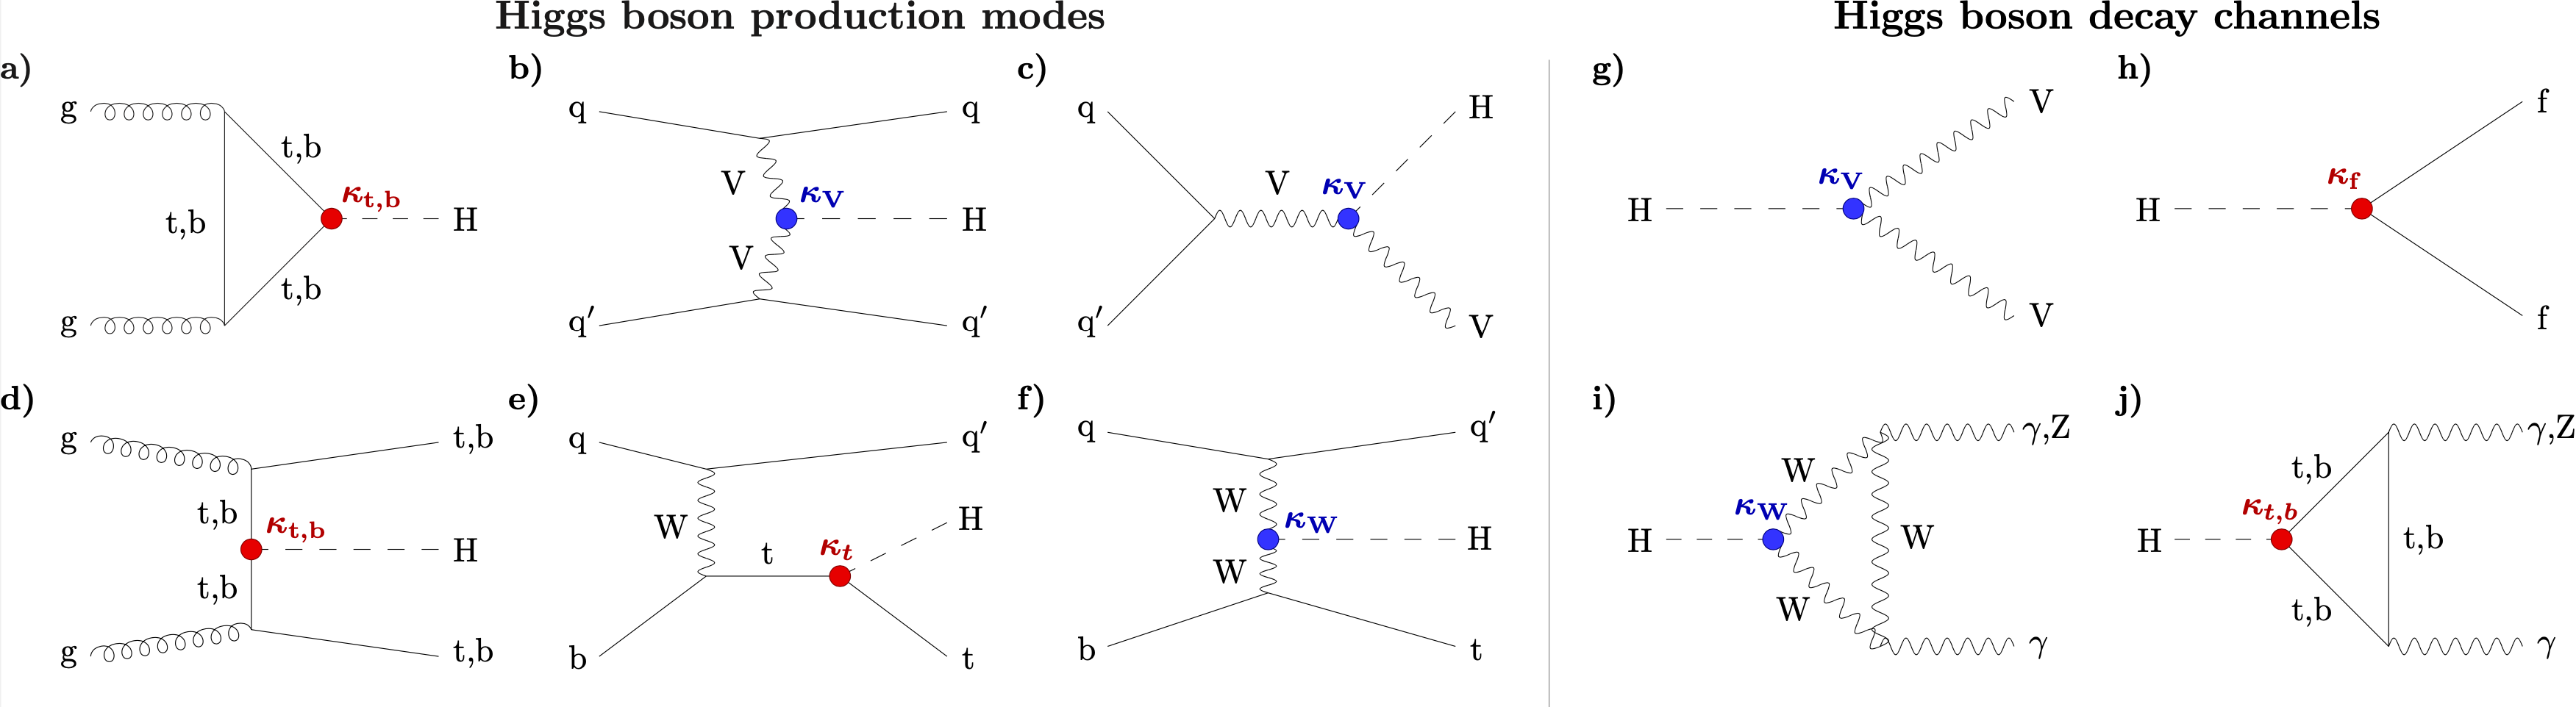
\includegraphics[width=\textwidth]{figures/01-SM-03-SM/higgs/higgs_production.png}
	\caption{Single Higgs boson production modes and decay channels at the LHC, reproduced from Ref.~\cite{CMS:2022dwd}.}
	\label{fig:01_sm_higgs_production}
\end{figure}

\begin{figure}[ht]
	\centering
	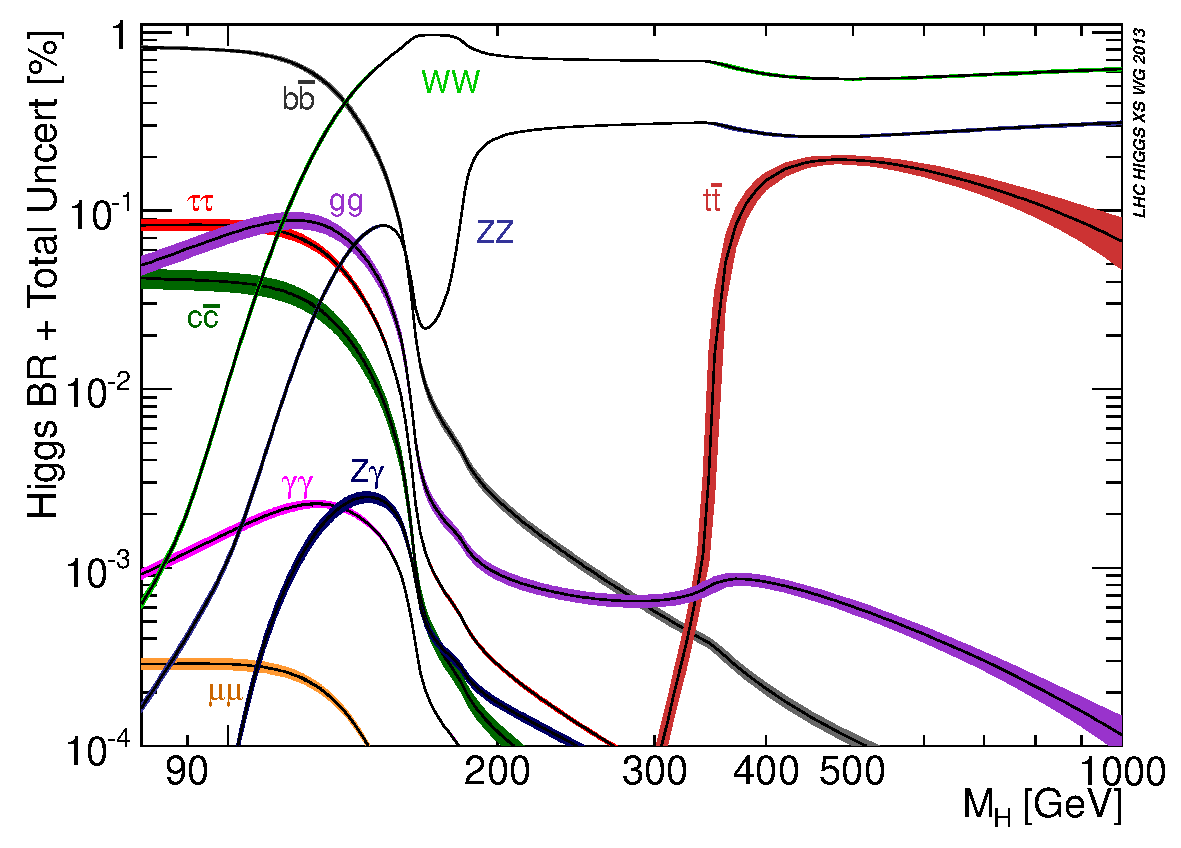
\includegraphics[width=0.8\textwidth]{figures/01-SM-03-SM/higgs/Higgs_BR_RECT.pdf}
	\caption{Higgs branching fractions predicted in the SM as a function of \mh (reproduced from Refs.~\cite{Dittmaier:2012vm,LHCHiggsCrossSectionWorkingGroup:2016ypw}).}
	\label{fig:01_sm_higgs_hbrs}
\end{figure}

The Higgs boson was initially observed by the CMS and ATLAS experiments in 2012 through a combination of several decay channels.
Since then, the two experiments have been making steady progress in the precise measurements of the various Higgs properties.
For example, Figure~\ref{fig:01_sm_higgs_constraints} shows the overall constraints on the Higgs to fermion and vector boson couplings and the Higgs mass by the CMS experiment.
Constraints are based on the $\kappa$-framework~\cite{LHCHiggsCrossSectionWorkingGroup:2013rie}, where $\kappa_X$ scales the Higgs-$X$ coupling strength with $\kappa_X = 1$ corresponding to the SM prediction.
Changes to the coupling strength due to new physics are thus generically captured by deviations from $\kappa_X = 1$.


\begin{figure}[ht]
	\centering
	\adjustbox{valign=m}{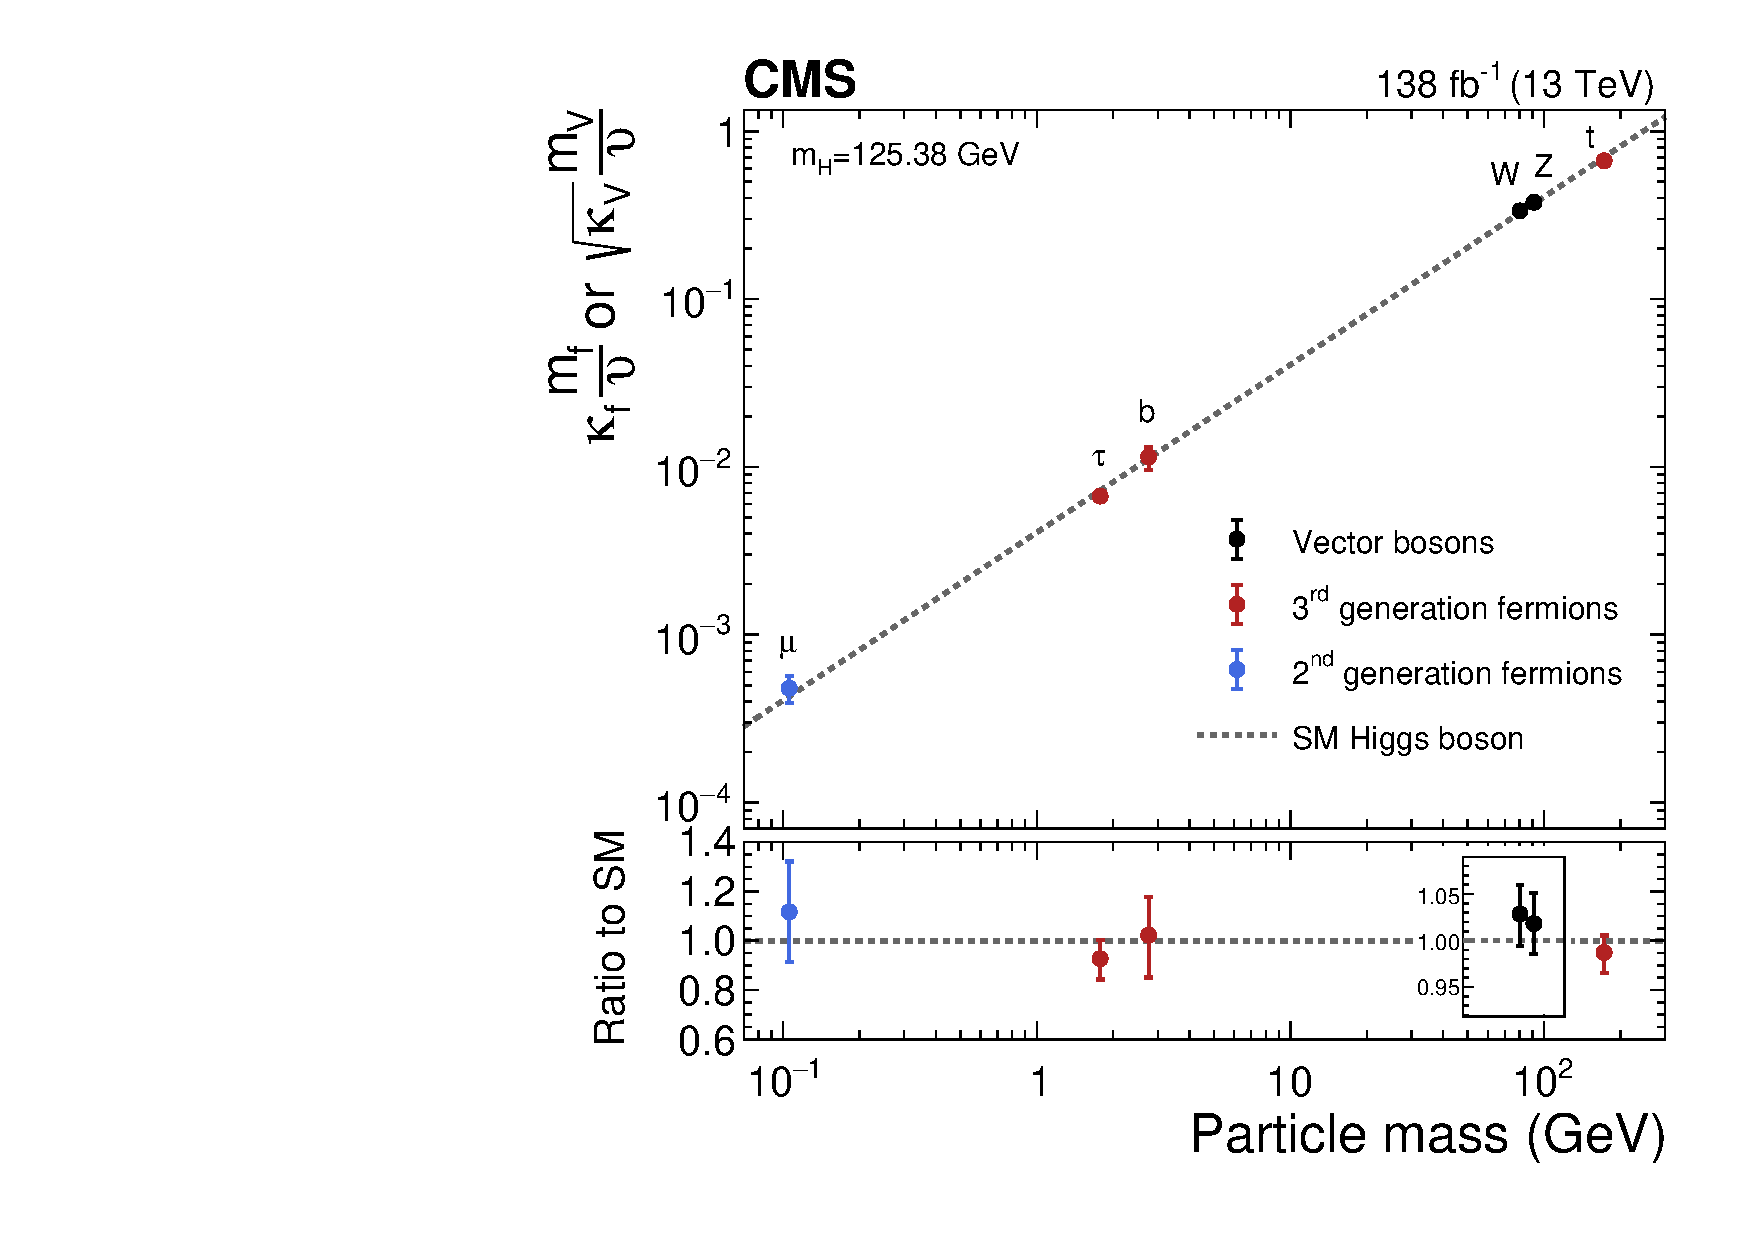
\includegraphics[width=0.49\textwidth]{figures/01-SM-03-SM/higgs/higgs_couplings.pdf}}
	\adjustbox{valign=m}{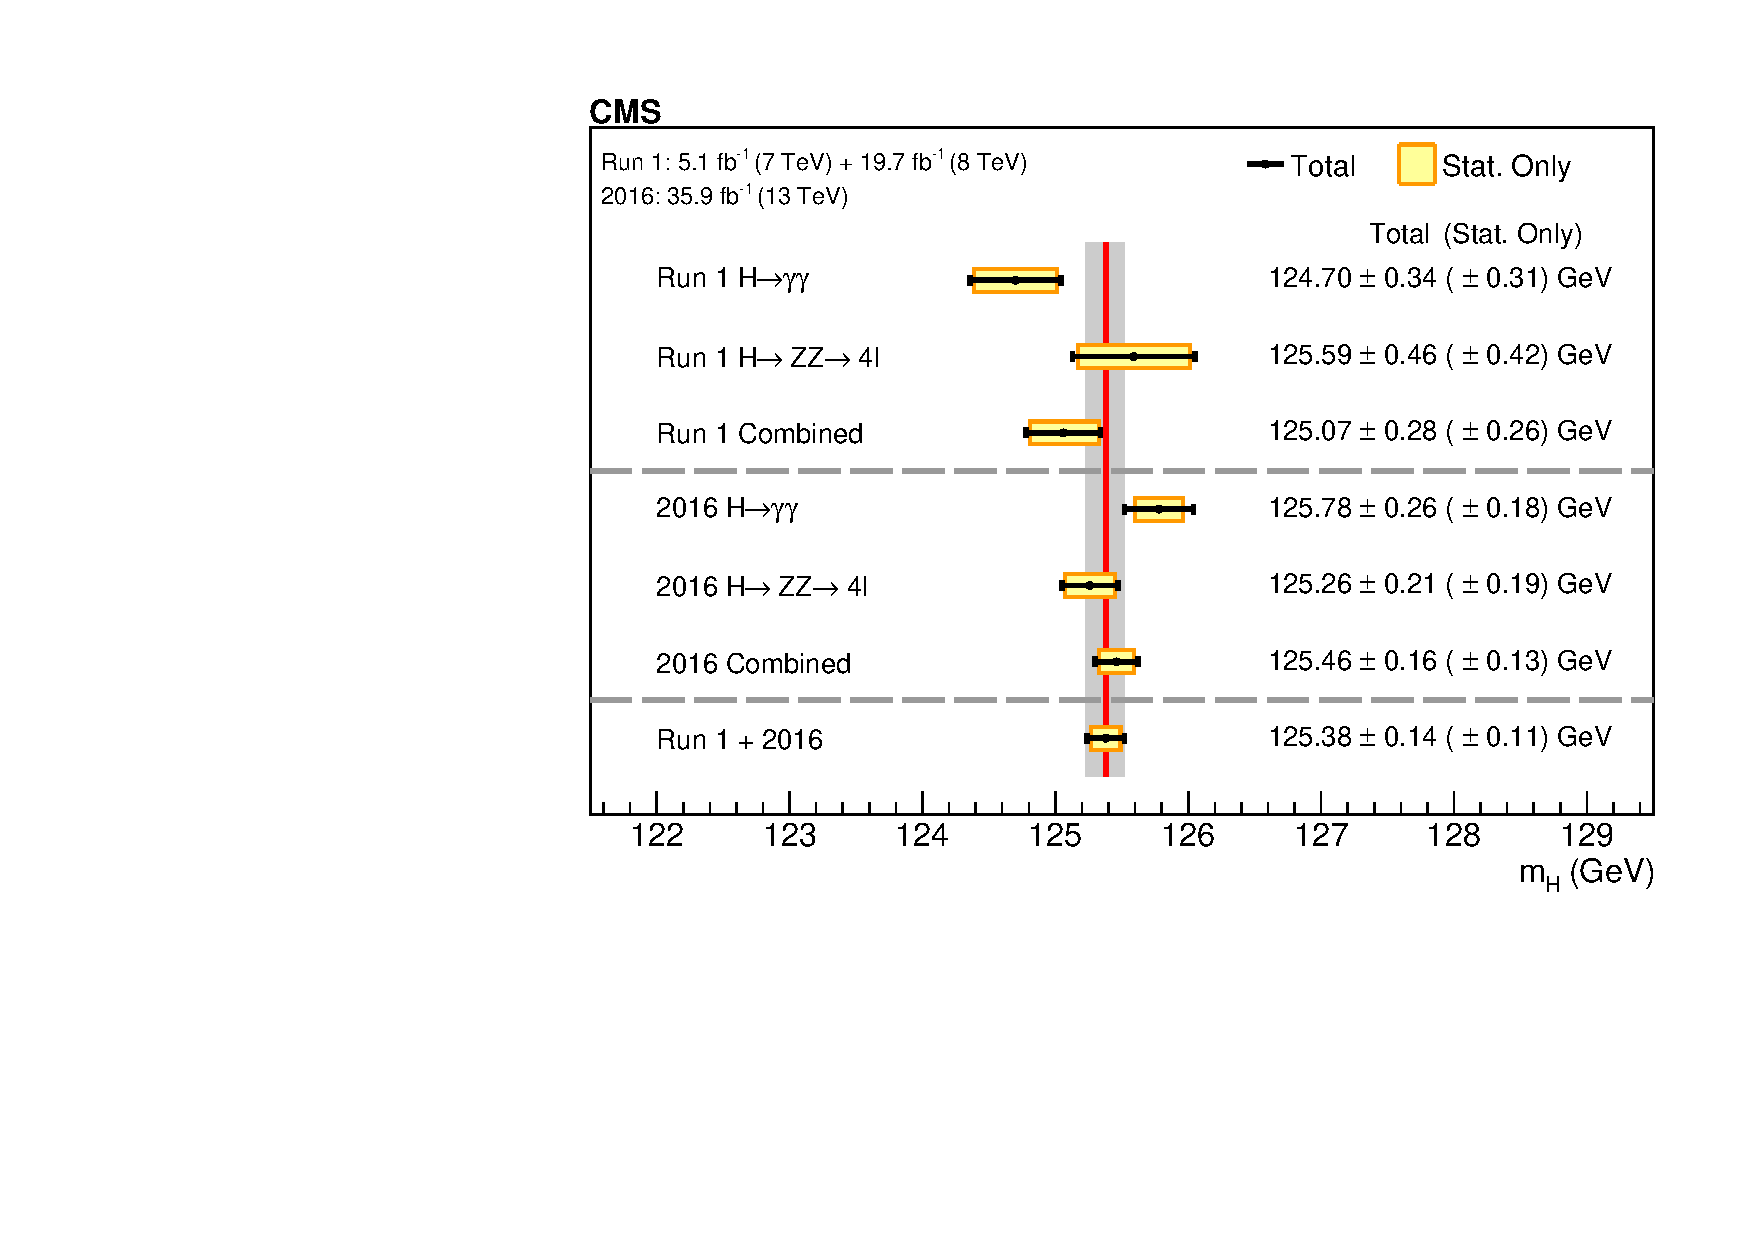
\includegraphics[width=0.49\textwidth]{figures/01-SM-03-SM/higgs/higgs_mass.pdf}}
	\caption{Constraints on Higgs to fermion and vector boson couplings, reproduced from Ref.~\cite{CMS:2022dwd} (left) and measurements of the Higgs mass, reproduced from Ref.~\cite{CMS:2020xrn} (right) by the CMS experiment.}
	\label{fig:01_sm_higgs_constraints}
\end{figure}


\subsection{Higgs pair production in the SM}
\label{sec:05_smhh}

Two couplings of the Higgs boson which have not been well-constrained are the trilinear Higgs self-coupling (\HHH), with coupling modifier \kapl, and the Higgs quartic coupling to vector bosons (\HHVV), with modifier $\kapvv$.
As discussed in Section~\ref{sec:01_sm_ew_ewsb} and illustrated in Figure~\ref{fig:01_sm_higgs_potential}, measuring the Higgs self-coupling in particular is necessary to fully characterize the Higgs potential, deviations to which could hint at BSM explanations to mysteries such as baryon asymmetry~\cite{Reichert:2017puo}.
As we describe below, both couplings can be probed exclusively through Higgs pair production (\HH), which is why it is a key physics target for the upcoming high-luminosity era of the LHC.

\begin{figure}[ht]
	\centering
	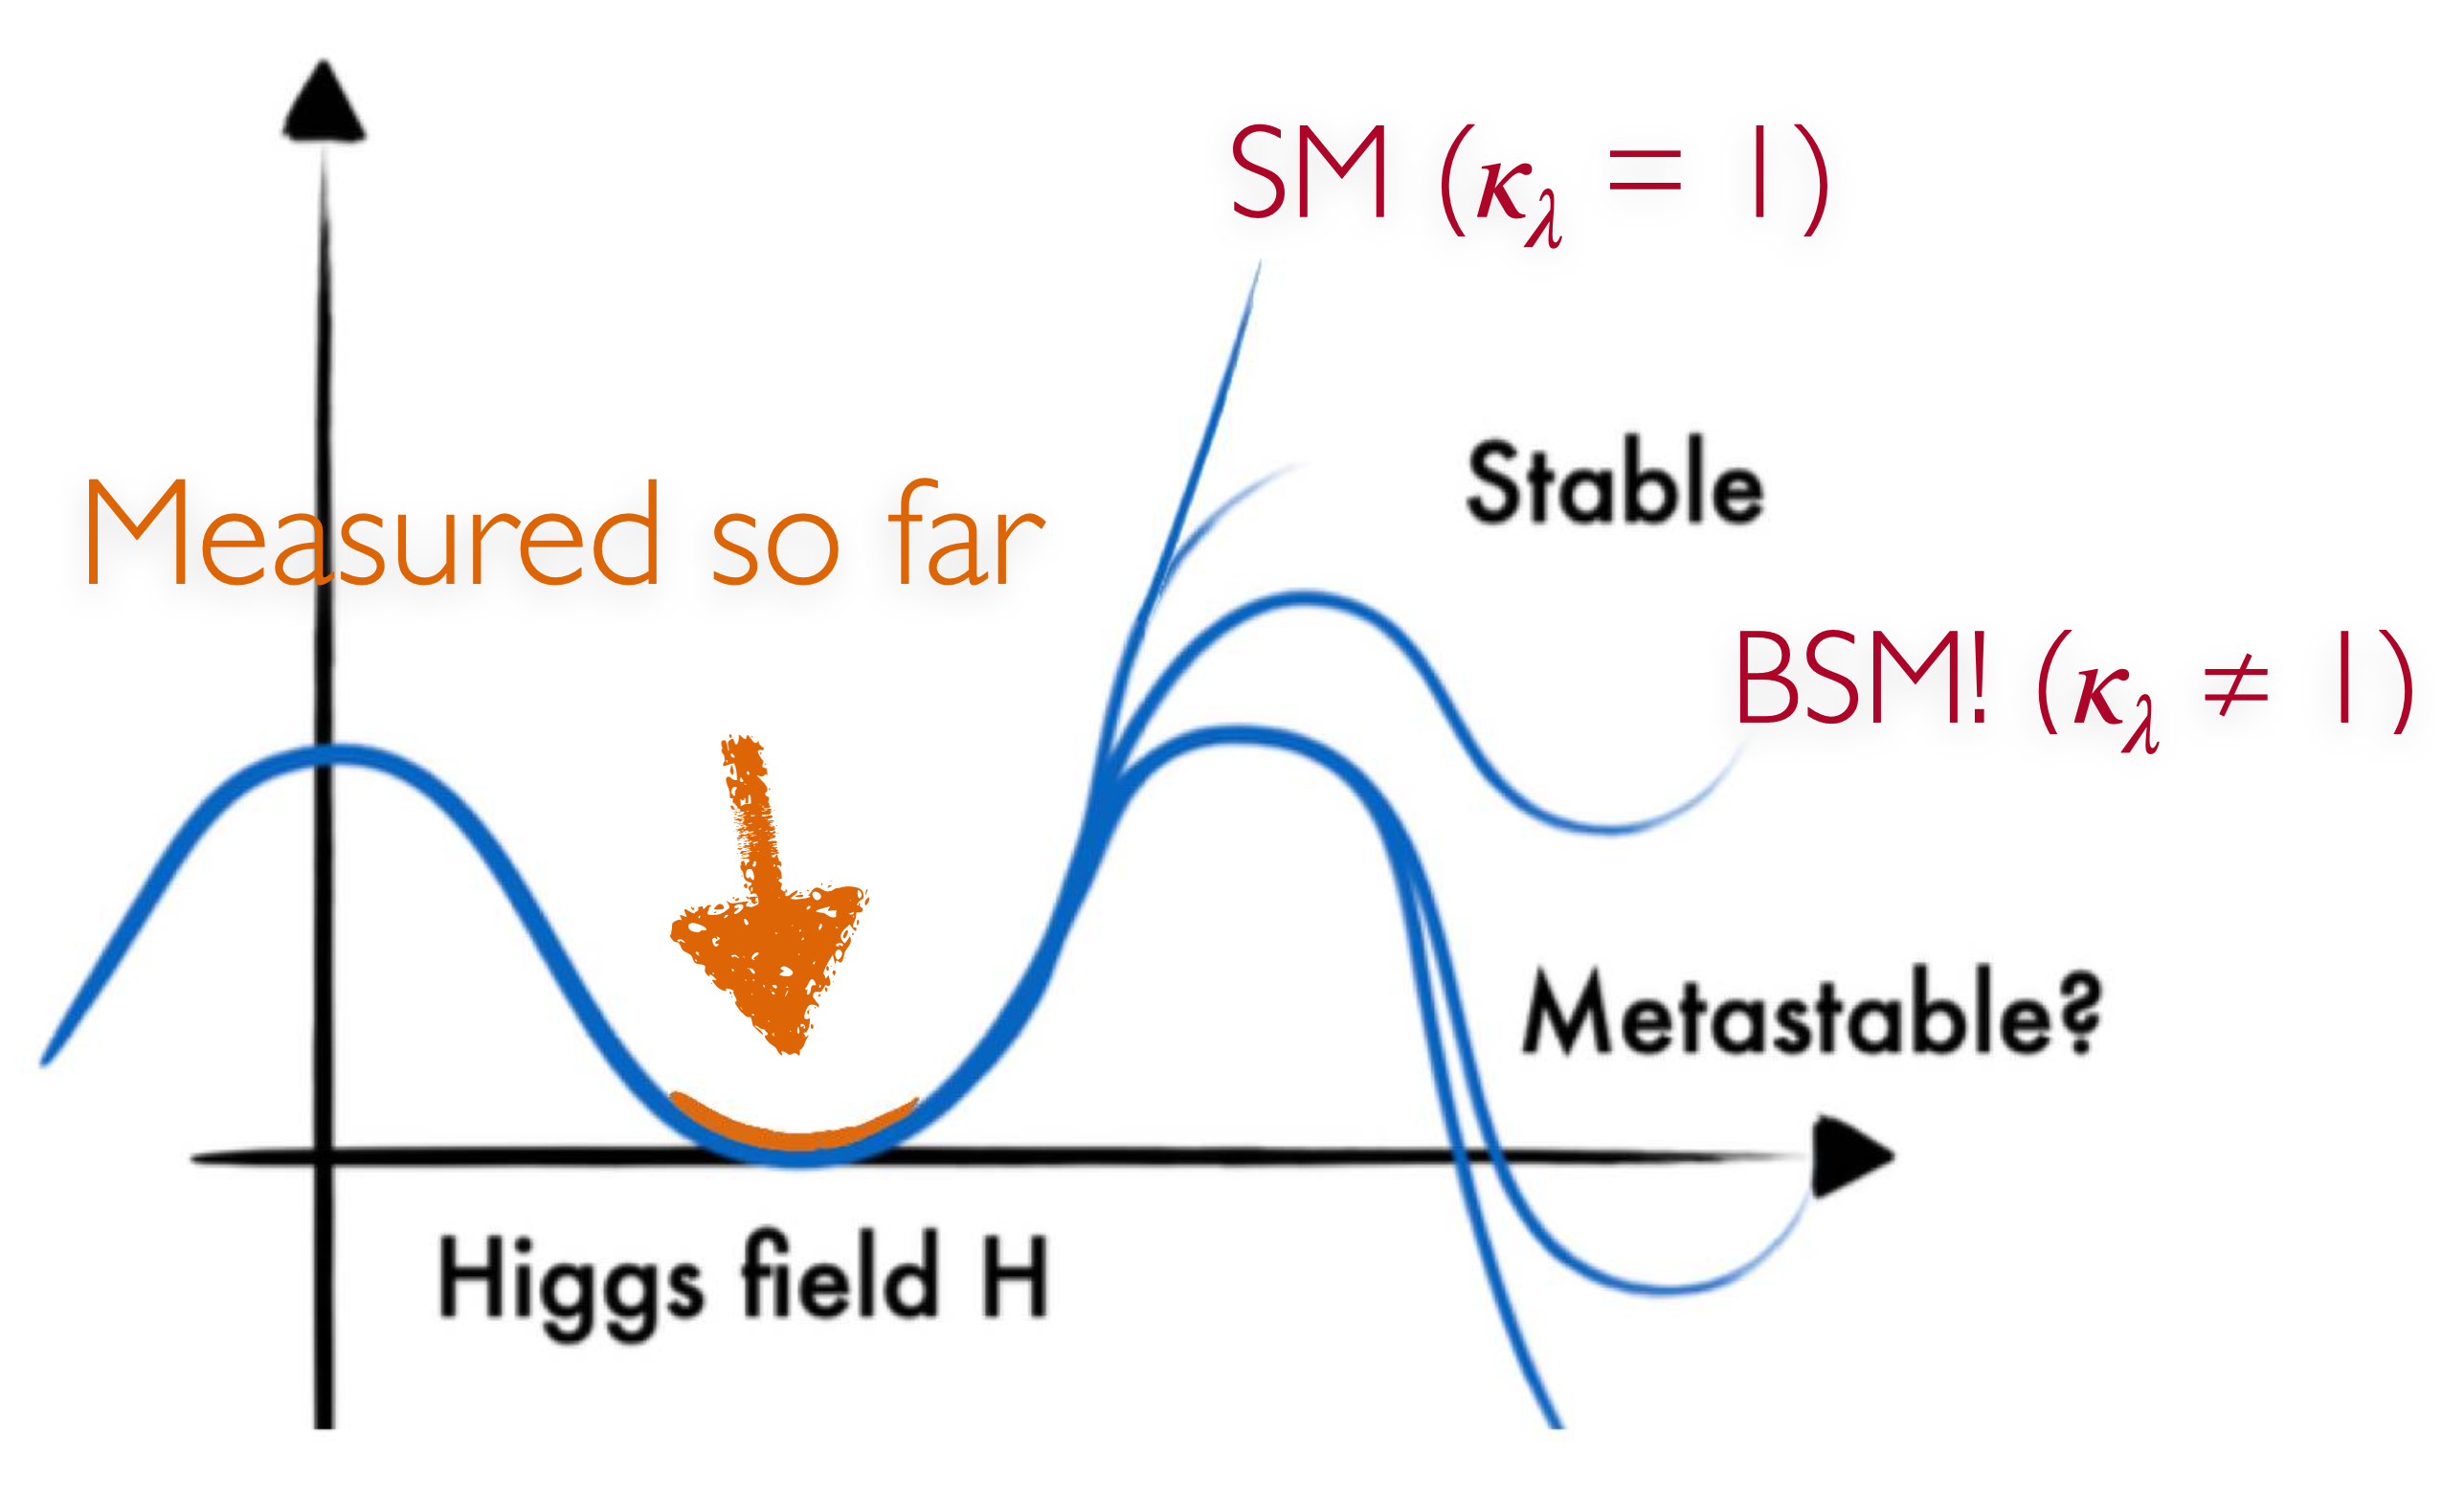
\includegraphics[width=0.5\textwidth]{figures/01-SM-03-SM/higgs/higgs_potential}
	\caption{Cartoon of the Higgs potential in the SM and potential deviations due to BSM physics.}
	\label{fig:01_sm_higgs_potential}
\end{figure}

\HH production in the SM occurs dominantly through gluon fusion (ggF), with a small production cross section $\sigma_{\mathrm{ggF}} = 31.05^{+2.2\%}_{-5.0\%} \pm 3\% (\textrm{PDF}+\alpS)^{+4\%}_{-18\%} (m_\PQt)\unit{fb}$~\cite{Grazzini:2018bsd,Baglio:2020wgt} at a center of mass energy of 13\TeV and $\mH = 125\GeV$, and subdominantly through vector boson fusion (VBF), with a smaller production cross section $\sigma_{\mathrm{VBF}} = 1.726^{+0.03\%}_{-0.04\%} \pm 2.1\% (\textrm{PDF}+\alpS)\unit{fb}$~\cite{LHCHiggsCrossSectionWorkingGroup:2016ypw}.
At leading order, the ggF production mode has contributions from diagrams that involve the trilinear \HHH Higgs self-coupling and the emission of two Higgs bosons through a top quark loop, while the VBF production mode has contributions from three diagrams involving the trilinear \HHH, \HVV, and quartic \HHVV couplings (Figures~\ref{fig:05_feynmanggf} and~\ref{fig:05_feynmanvbf}).
It also features the distinct final state signature of two, typically forward, jets in addition to the two Higgs bosons.

\begin{figure}[htb] %[ht]
    \centering
    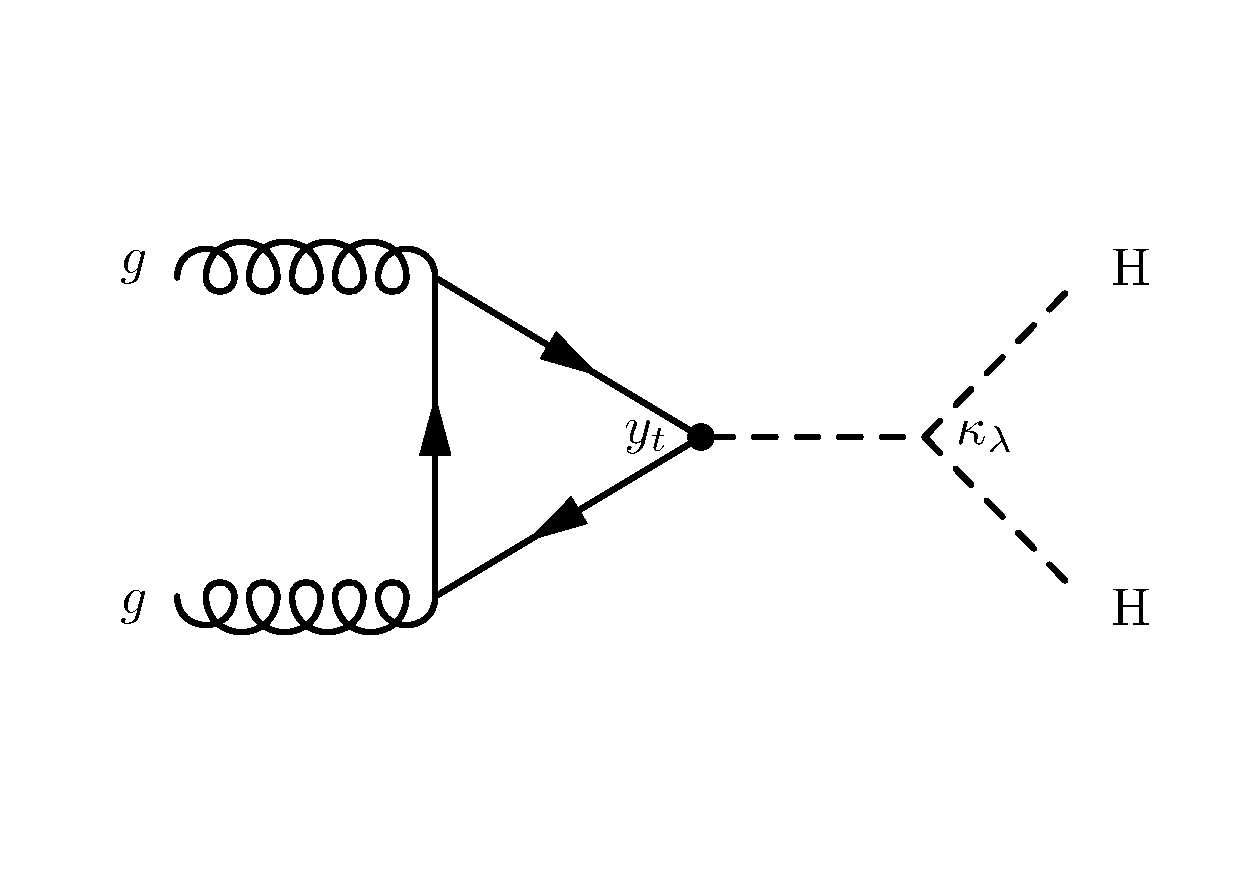
\includegraphics[width=0.4\textwidth]{figures/05-HH/production/diagrams/feynman_02.pdf}
    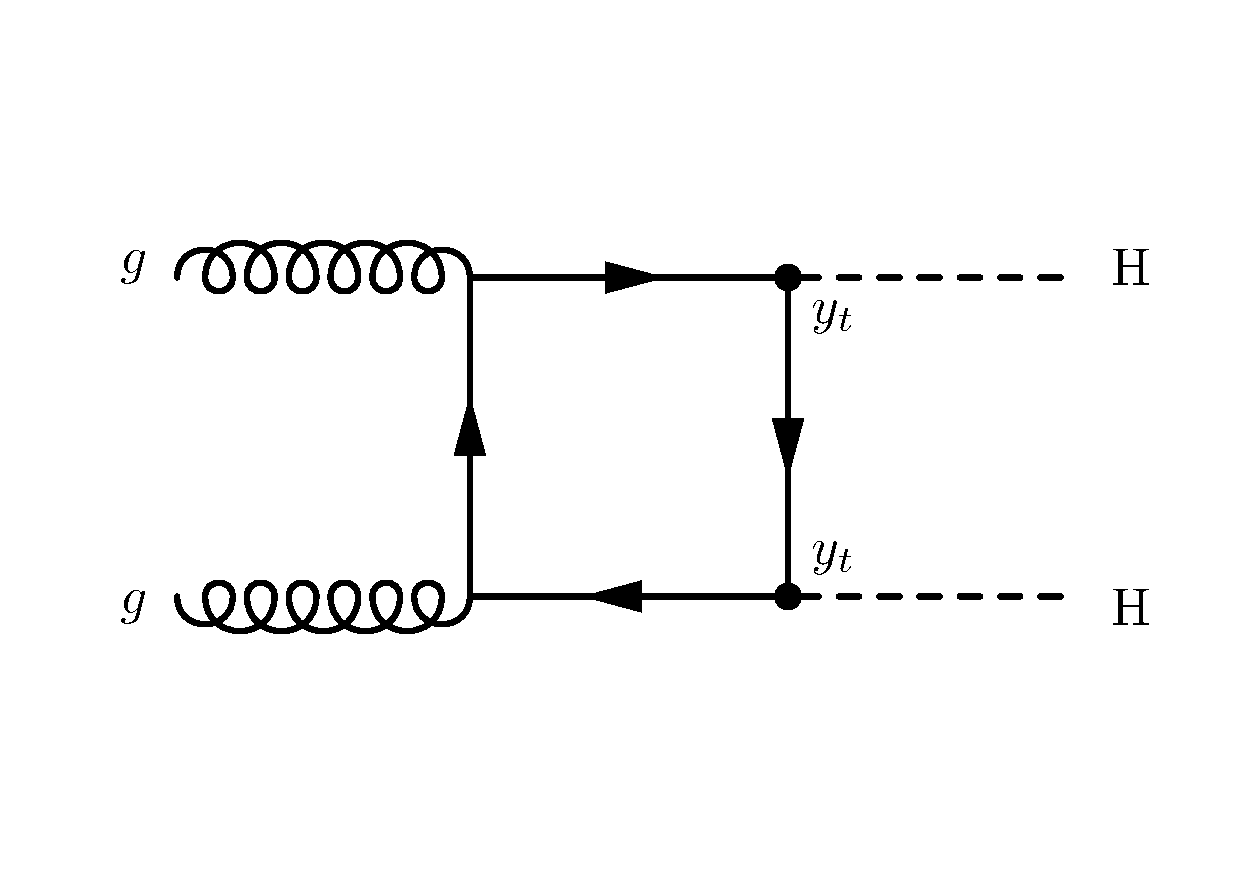
\includegraphics[width=0.4\textwidth]{figures/05-HH/production/diagrams/feynman_01.pdf}
    \caption{Leading-order diagrams for nonresonant \HH production via gluon gluon fusion.}
    \label{fig:05_feynmanggf}
\end{figure}  
    
\begin{figure}[htb]
    \centering
    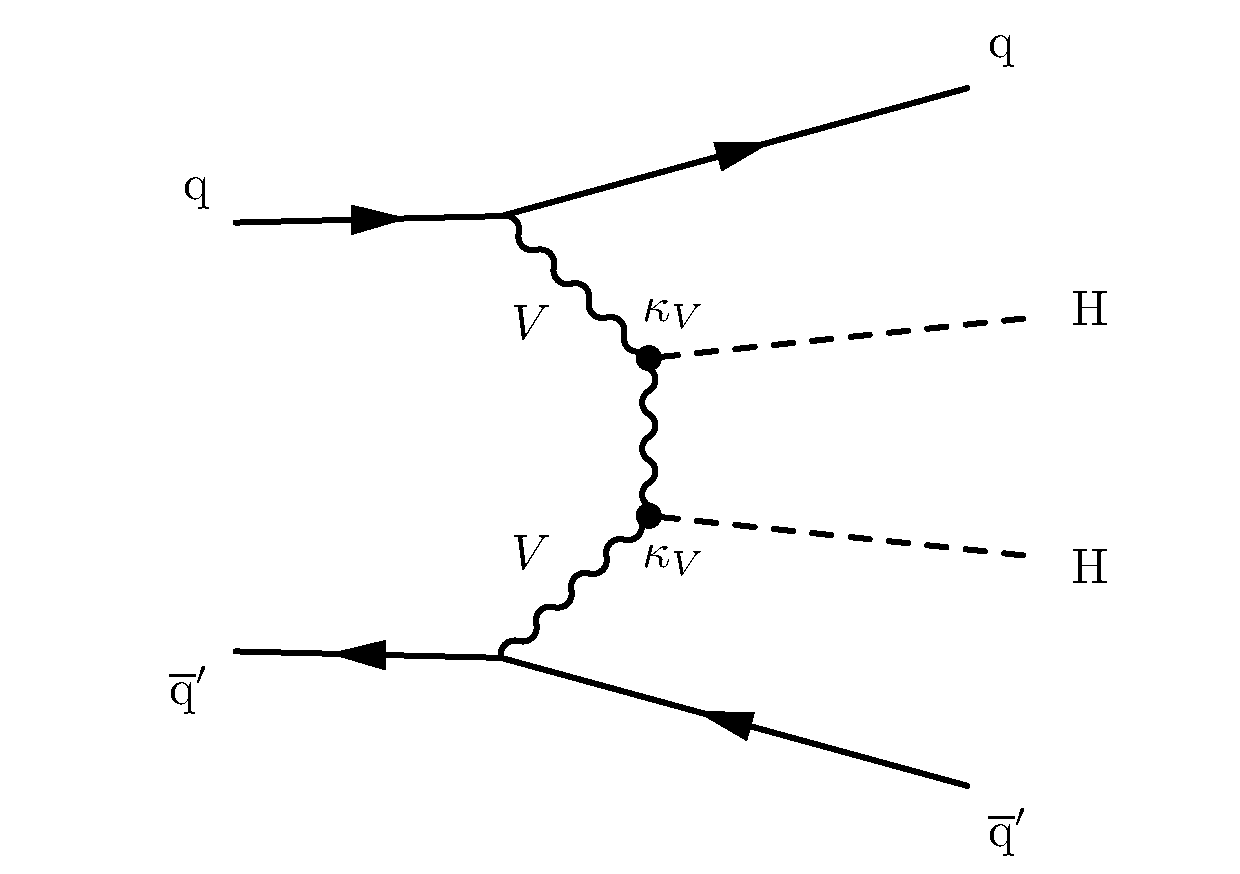
\includegraphics[width=0.32\textwidth]{figures/05-HH/production/diagrams/feynman_04.pdf}
    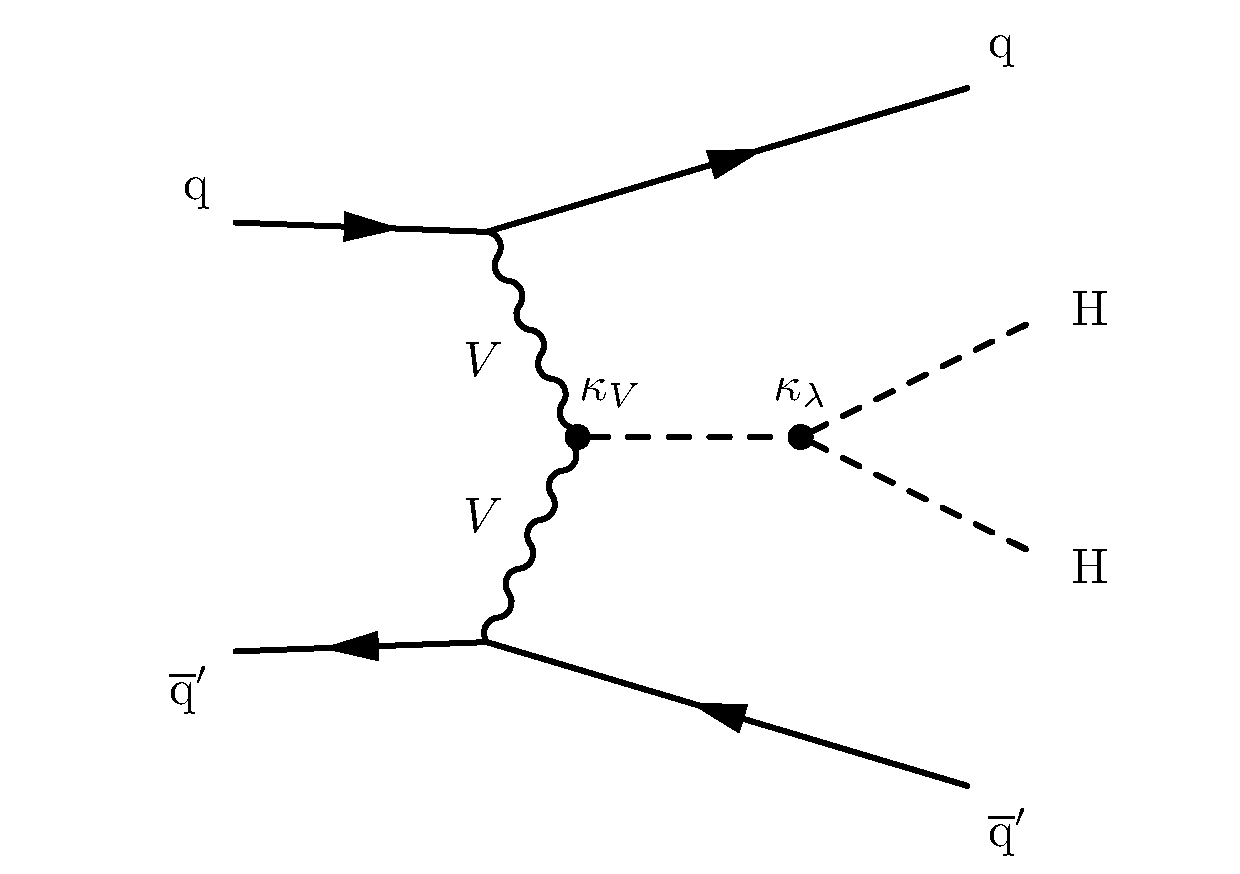
\includegraphics[width=0.32\textwidth]{figures/05-HH/production/diagrams/feynman_05.pdf}
    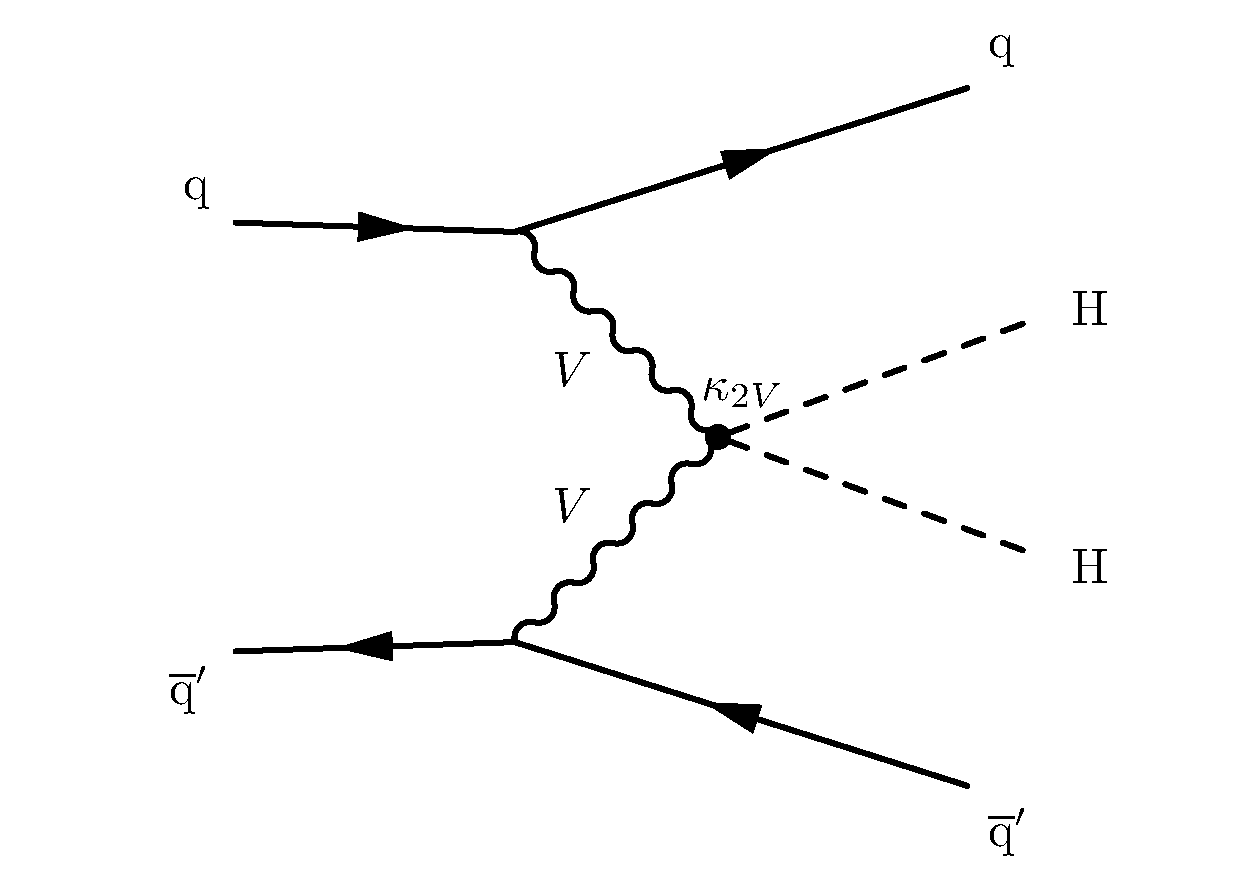
\includegraphics[width=0.32\textwidth]{figures/05-HH/production/diagrams/feynman_03.pdf}
    \caption{Leading-order diagrams for nonresonant \HH production via vector boson fusion.
    In this chapter, we refer to the left-most VBF diagram as the $(\HVV)^2$ and the right-most as the $\HHVV$ diagram.}
    \label{fig:05_feynmanvbf}
\end{figure} 

The production cross section and kinematic properties of the \HH system are altered if values of the Higgs self-coupling, the top Yukawa coupling, and/or the quartic \HHVV coupling are modified due to beyond the SM (BSM) effects.
Notably, at the energy scale of the LHC, the leading contribution to the VBF production amplitude is the scattering of longitudinal vector bosons, which scales as $\sim m_{\PH\PH}^2 (\kapvv - \kappa_{\PV}^2)$~\cite{Bishara:2016kjn}, where, as above, \kapl, $\kapvv$, and $\kapv$ are defined to be multiplicative modifiers of the \HHH, \HHVV, and \HVV couplings from their SM values, respectively.

In the SM, with $\kapvv = \kapv = 1$, VBF production is suppressed since the left-most $(\HVV)^2$ and right-most \HHVV VBF diagrams in Figure~\ref{fig:05_feynmanvbf} cancel; however, BSM deviations to \HHVV can spoil the cancelation, significantly enhancing this mode.
This departure from the SM could be more visible at high energies, as illustrated in Figure~\ref{fig:05_intro_mhh}, which shows the increase and shift towards higher \mHH of the differential VBF \HH production cross section for enhanced and reduced \kapvv values.
Thus, measuring high-\mHH nonresonant VBF \HH production, with both Higgs bosons highly Lorentz-boosted, is a powerful probe of the \HHVV coupling.

\begin{figure}[ht]
    \centering
    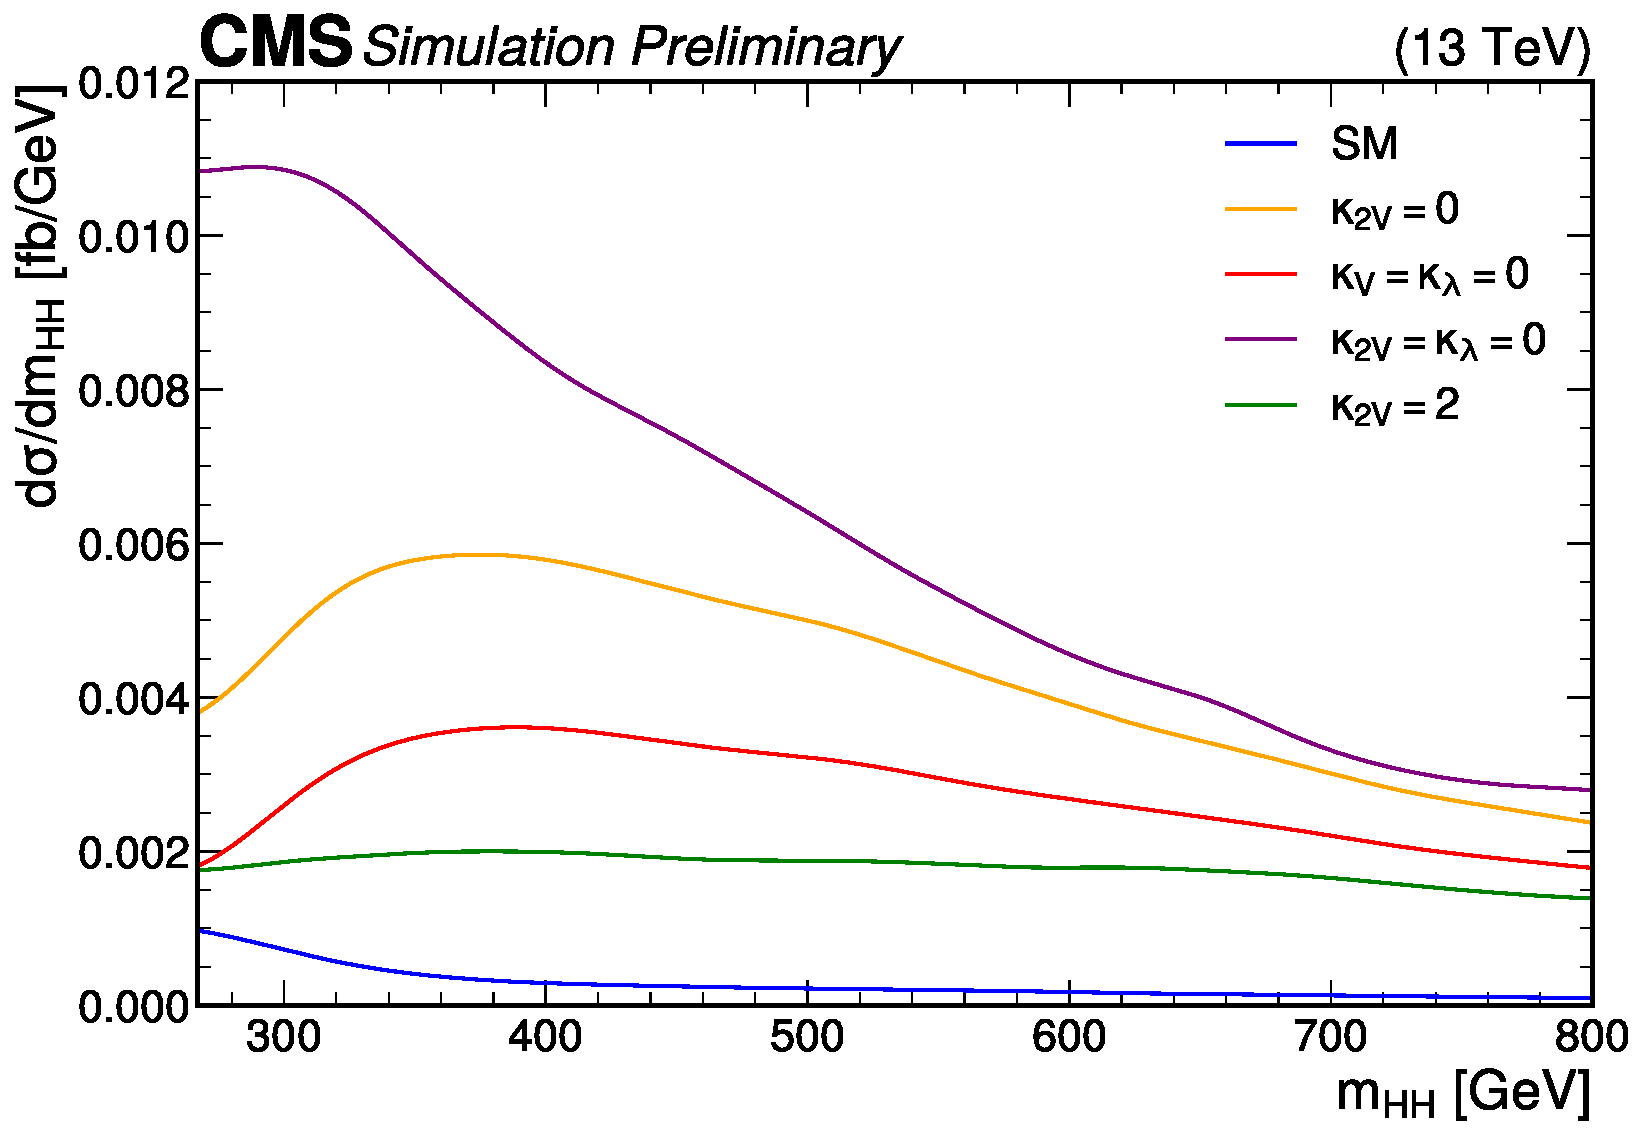
\includegraphics[width=0.7\textwidth]{figures/05-HH/production/diagrams_prelim.pdf}
    \caption{Differential cross section at $13\TeV$ center of mass for VBF \HH production as a function of the invariant mass of the \HH system (\mHH) for different diagrams and couplings.}
    \label{fig:05_intro_mhh}
\end{figure}

This is evidenced by the current \kapvv constraint in CMS being dominated by the search for boosted \HH in the \bbbb channel, with an observed (expected) 95\% confidence level (\CL) constraint of $[0.6, 1.4]$ ($[0.7, 1.4]$), excluding $\kapvv = 0$ for the first time~\cite{CMS:2022gjd}.
This is followed by CMS searches in the resolved \bbbb~\cite{CMS:2022cpr} and \bbtautau~\cite{CMS:2022hgz} channels, with constraints of $[-0.1, 2.2]$ ($[-0.4, 2.5]$) and $[-0.4, 2.6]$ ($[-0.6, 2.8]$), respectively.
Similarly, the strongest \kapvv constraint from the ATLAS experiment is from the boosted \bbbb search~\cite{ATLAS-CONF-2024-003}, with an observed (expected) 95\% \CL constraint of $[0.55, 1.49]$ ($[0.3, 1.7]$).

The success of searches in the boosted \bbbb channel motivates further exploration of high-\mHH \HH production.
This dissertation presents the first search in the all-hadronic \bbvv channel, where one Higgs boson decays to \bbbar while the other to \ww or \zz, where $\PW\to\qqbar$ and $\PZ\to\qqbar$.
The branching fractions for the \bbbar and all-hadronic \VV decays are $0.58$ and $0.11$ respectively, for a total branching fraction $\mathcal{B}(\HHbbVVq) = 2  \cdot0.58\cdot 0.11 = 0.13$, which is the second largest behind \bbbb.
The analysis primarily aims to constrain \kapvv and also sets an exclusion limit on the inclusive \HH production cross-section.
It is not expected to be sensitive to \kapl because of the focus on the high-\mHH regime.

Another benefit of the high-\mHH regime is the significantly reduced QCD multijet background, which otherwise makes such all-hadronic searches extremely challenging.
Because of the two Higgs bosons' high Lorentz-boosts, this regime also features the unique experimental signature of the \bbbar and \VVq decays each being reconstructed as single wide-radius jets.
Such merged \hbb jets have been identified to great effect in CMS using deep neural networks (DNNs)~\cite{CMS:2023tlv, CMS:2022gjd}, but attaining similar signal versus background discrimination for \hvv jets remains an open challenge.
To this end, we introduce a new attention-based DNN, referred to as the global particle transformer (GloParT) to not only enable this search but open new possibilities for searches in boosted-\VV channels as well (Chapter~\ref{sec:05_jet_tagging}).

\subsection{Experimental status of \HH measurements with CMS}
\label{sec:05_smhh_golden_channels}

\begin{figure}[ht]
    \centering
    % \captionsetup{justification=centering}
    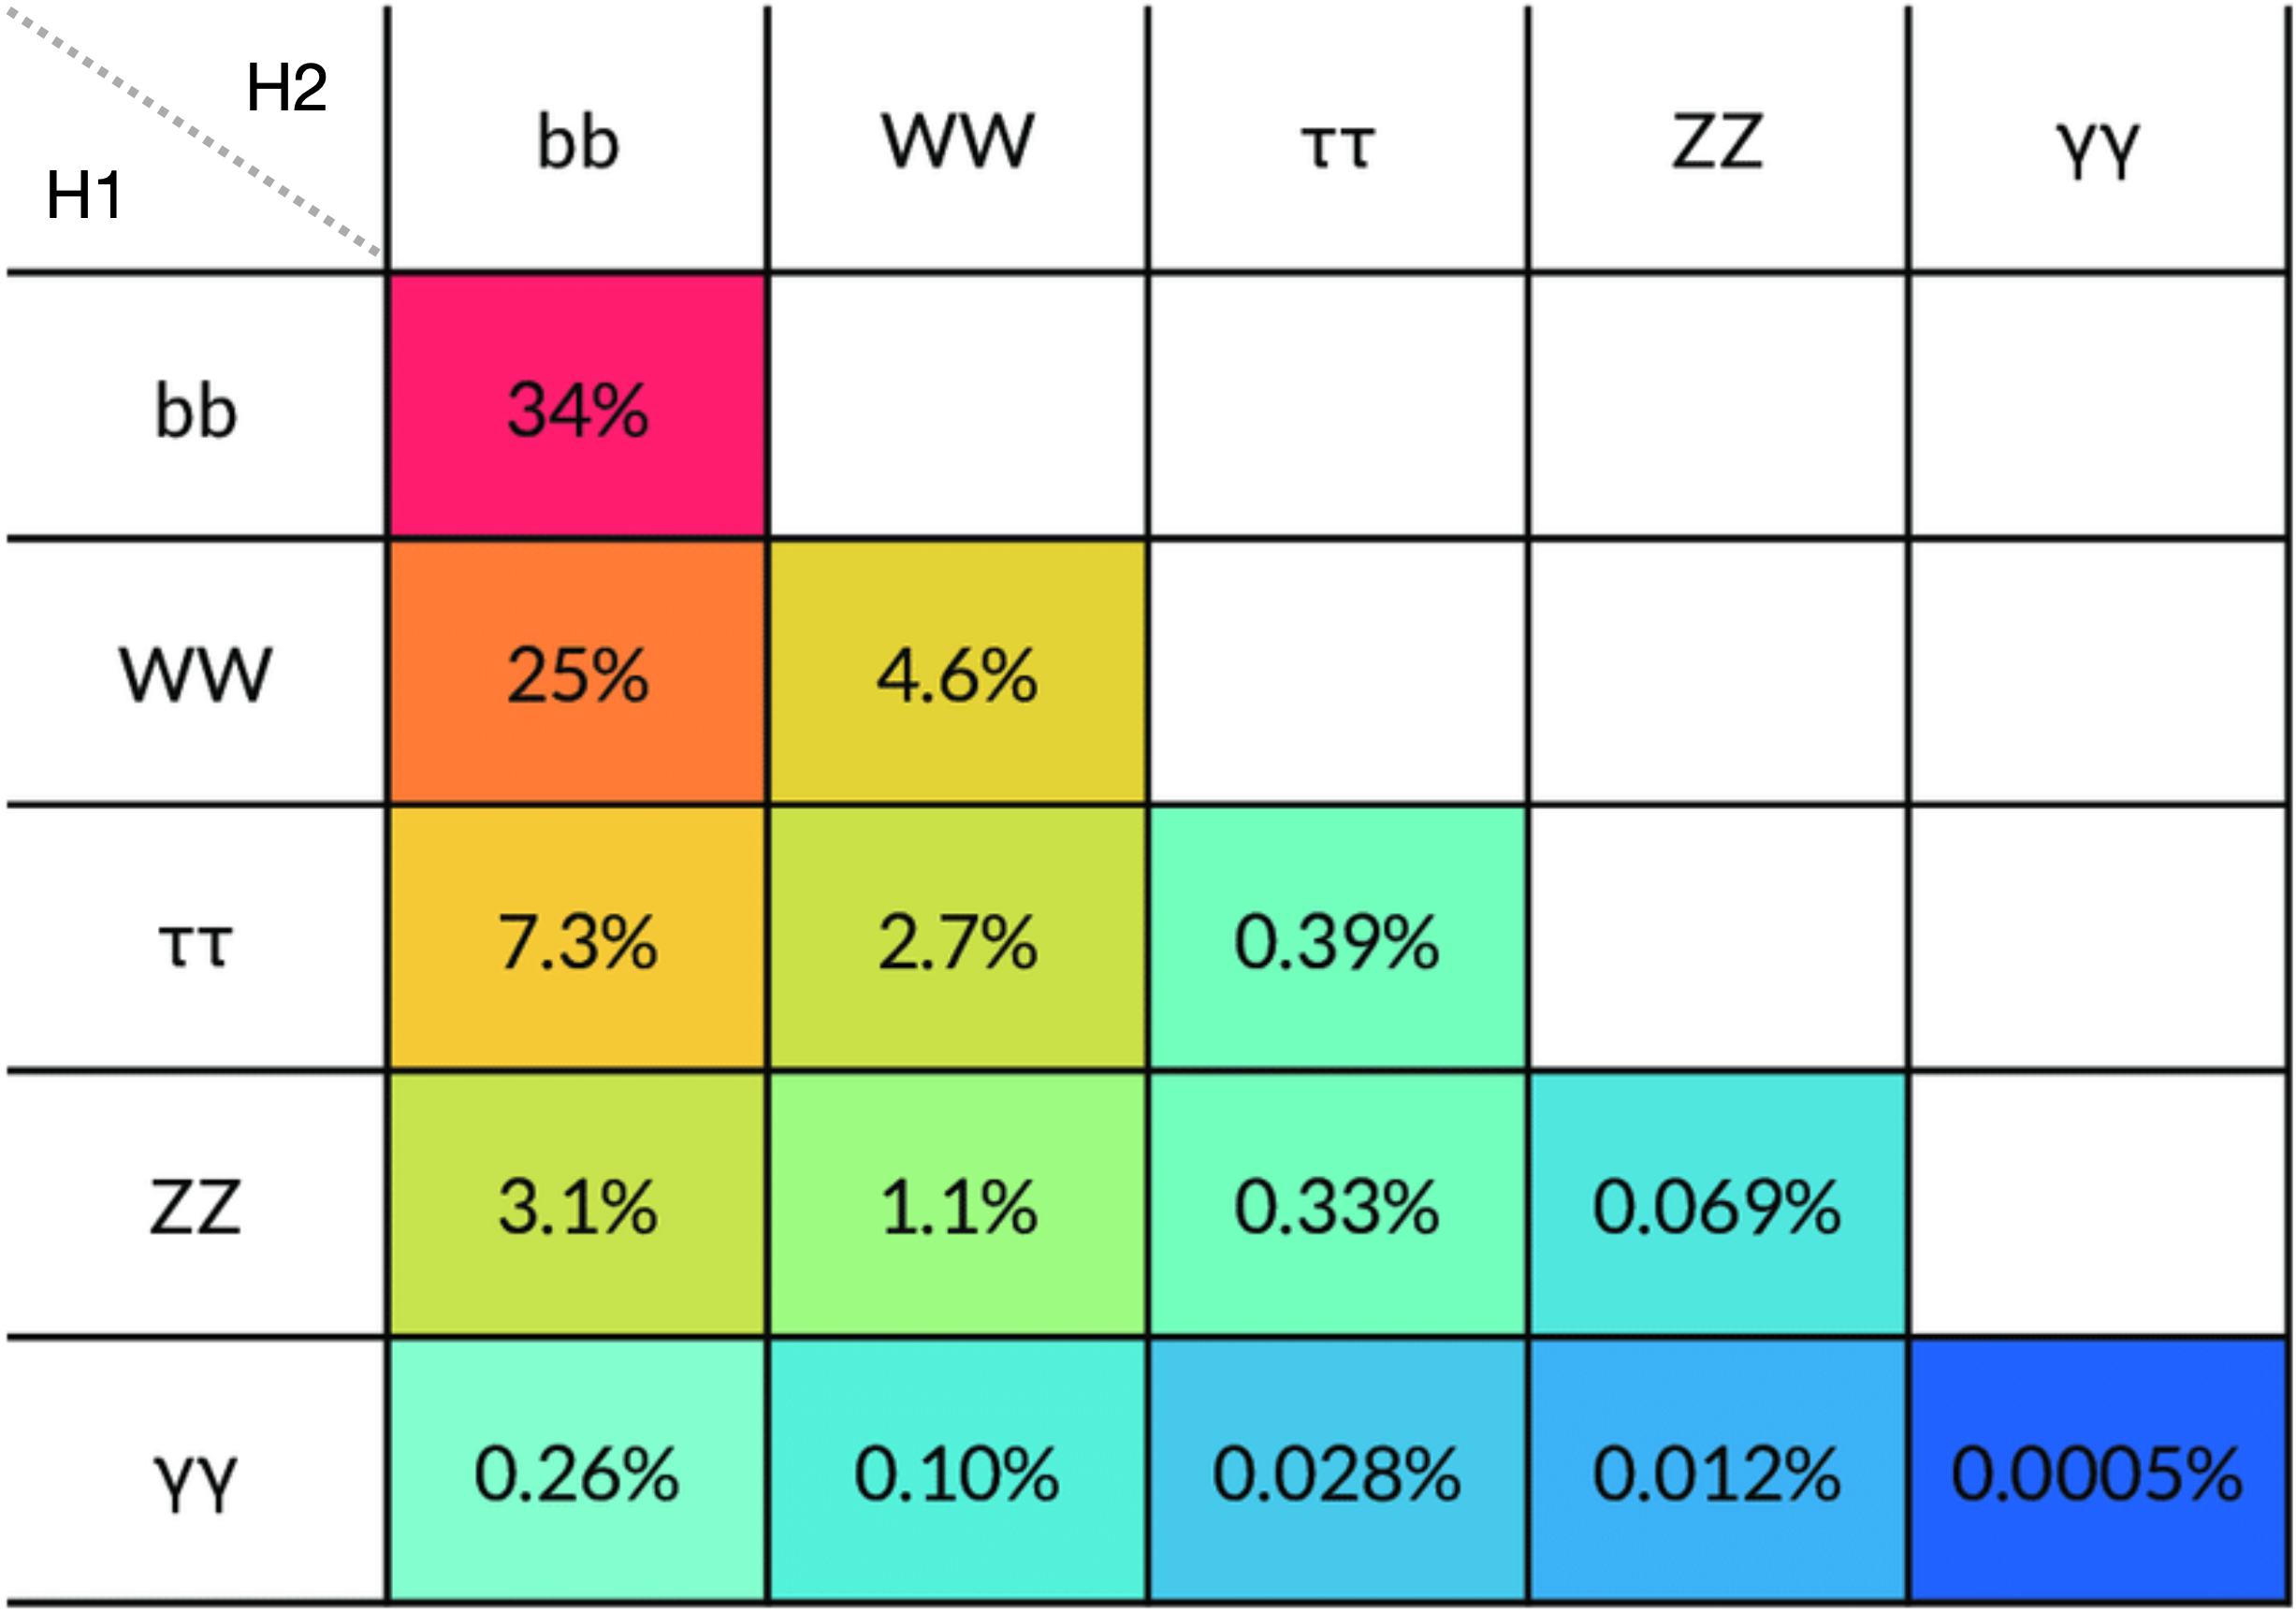
\includegraphics[width=0.6\textwidth]{figures/05-HH/CMS-results/HHBRs.png}
    \caption{\HH decays and their respective branching fractions (reproduced from Ref.~\cite{Veatch:2022uzz}).}
    \label{fig:05_hhbrs}
\end{figure}

The decays and branching fractions (BFs) of the Higgs boson pairs are shown in Figure~\ref{fig:05_hhbrs}.
Three of these final states have emerged as experimental ``golden channels'' --- the channels expected to yield the highest signal-to-background-events ratio for SM \HH production:
\begin{itemize}
    \item \bbbb:\quad This channel has the highest BF ($34\%$) and, despite the large QCD multijet background due to the all-hadronic final state, it benefits from unique signatures of heavy-flavor \Pb-jets, such as the presence of secondary vertices and displaced tracks due to the long lifetimes of \Pb-hadrons.
    Both the resolved~\cite{CMS:2022cpr} and boosted~\cite{CMS:2022gjd} Run 2 CMS analyses (Figure~\ref{fig:05_bbbb_run2}) have been highly effective, with the latter benefitting from the high BF of this decay mode, the exponential reduction of the QCD multijet background in the boosted regime, and significant recent advances in \bbbar-jet classification and reconstruction (as will be discussed in Chapter~\ref{sec:05_jet_tagging}). 
    \item \bbtautau:\quad This has an intermediate BF of $7\%$ but relatively lower background of primarily Drell-Yan ($\PZ/\PGg^*$), top quark pair production (\ttbar), and QCD multijet events (Figure~\ref{fig:05_bbtautau}, reproduced from Ref.~\cite{CMS:2022hgz}).
    It benefits from similar deep learning techniques for \Pb-jet tagging, and targets all-hadronic ($\PGt_h\PGt_h$) and semi-leptonic ($\PGt_h\PGt_e$ or $\PGt_h\PGt_\mu$) \PGt-lepton decays using a variety of traditional and ML techniques.
    \item \bbgg:\quad Despite the small BF ($0.3\%$) of this channel, the $\PH\to\PGg\PGg$ decay provides a clean experimental signature with a sharply peaking resonance over a small background of QCD multijet + $\PGg$ events (Figure~\ref{fig:05_bbgg}, from Ref.~\cite{CMS:2020tkr}).
\end{itemize}

More recently, the \bbww channel has been explored in the douple-lepton ($\Pl\Pl\nu\nu$) and single-lepton ($\Pl\nu\Pq\Pq$) \ww final states~\cite{CMS:2024rgy}, which have a large combined BF of $13.4\%$.
The former features a clean experimental signature of two opposite-sign leptons but a small BF of $2.6\%$, while the latter has the higher BF of 10.8\% but larger top quark background as well (Figure~\ref{fig:05_bbww}).
Because of this, the two channels have similar sensitivities to the \HH cross section.

\begin{figure}[htb!]
    \centering
    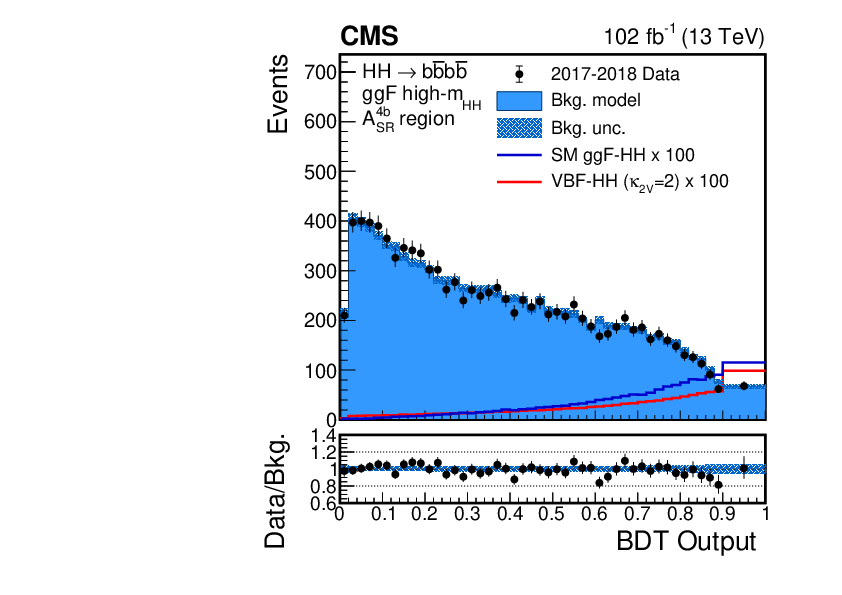
\includegraphics[trim=260pt 20pt 40pt 20pt, clip, width=0.31\textwidth]{figures/05-HH/CMS-results/4b/Figure_001-e.png}
    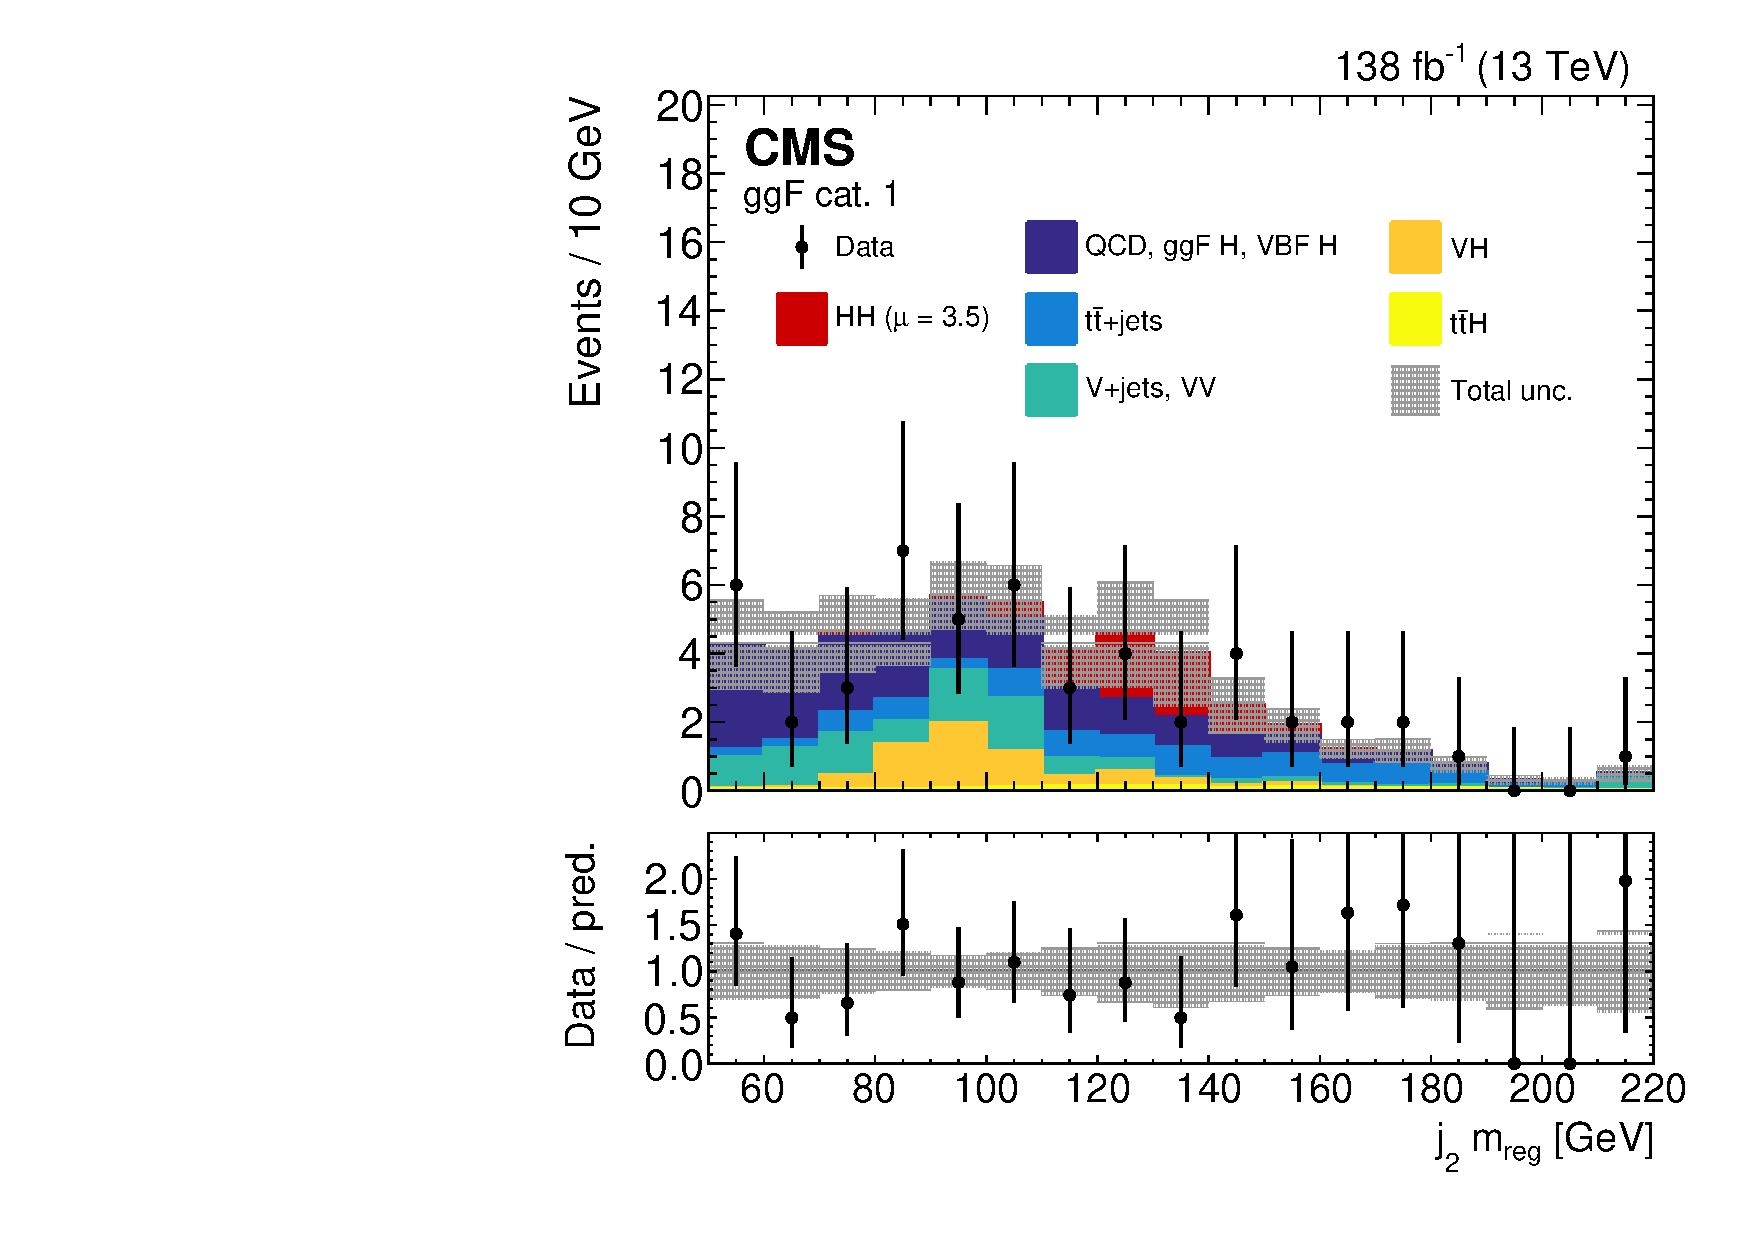
\includegraphics[width=0.33\textwidth]{figures/05-HH/CMS-results/4b/CMS-B2G-22-003_Figure_001.pdf}
    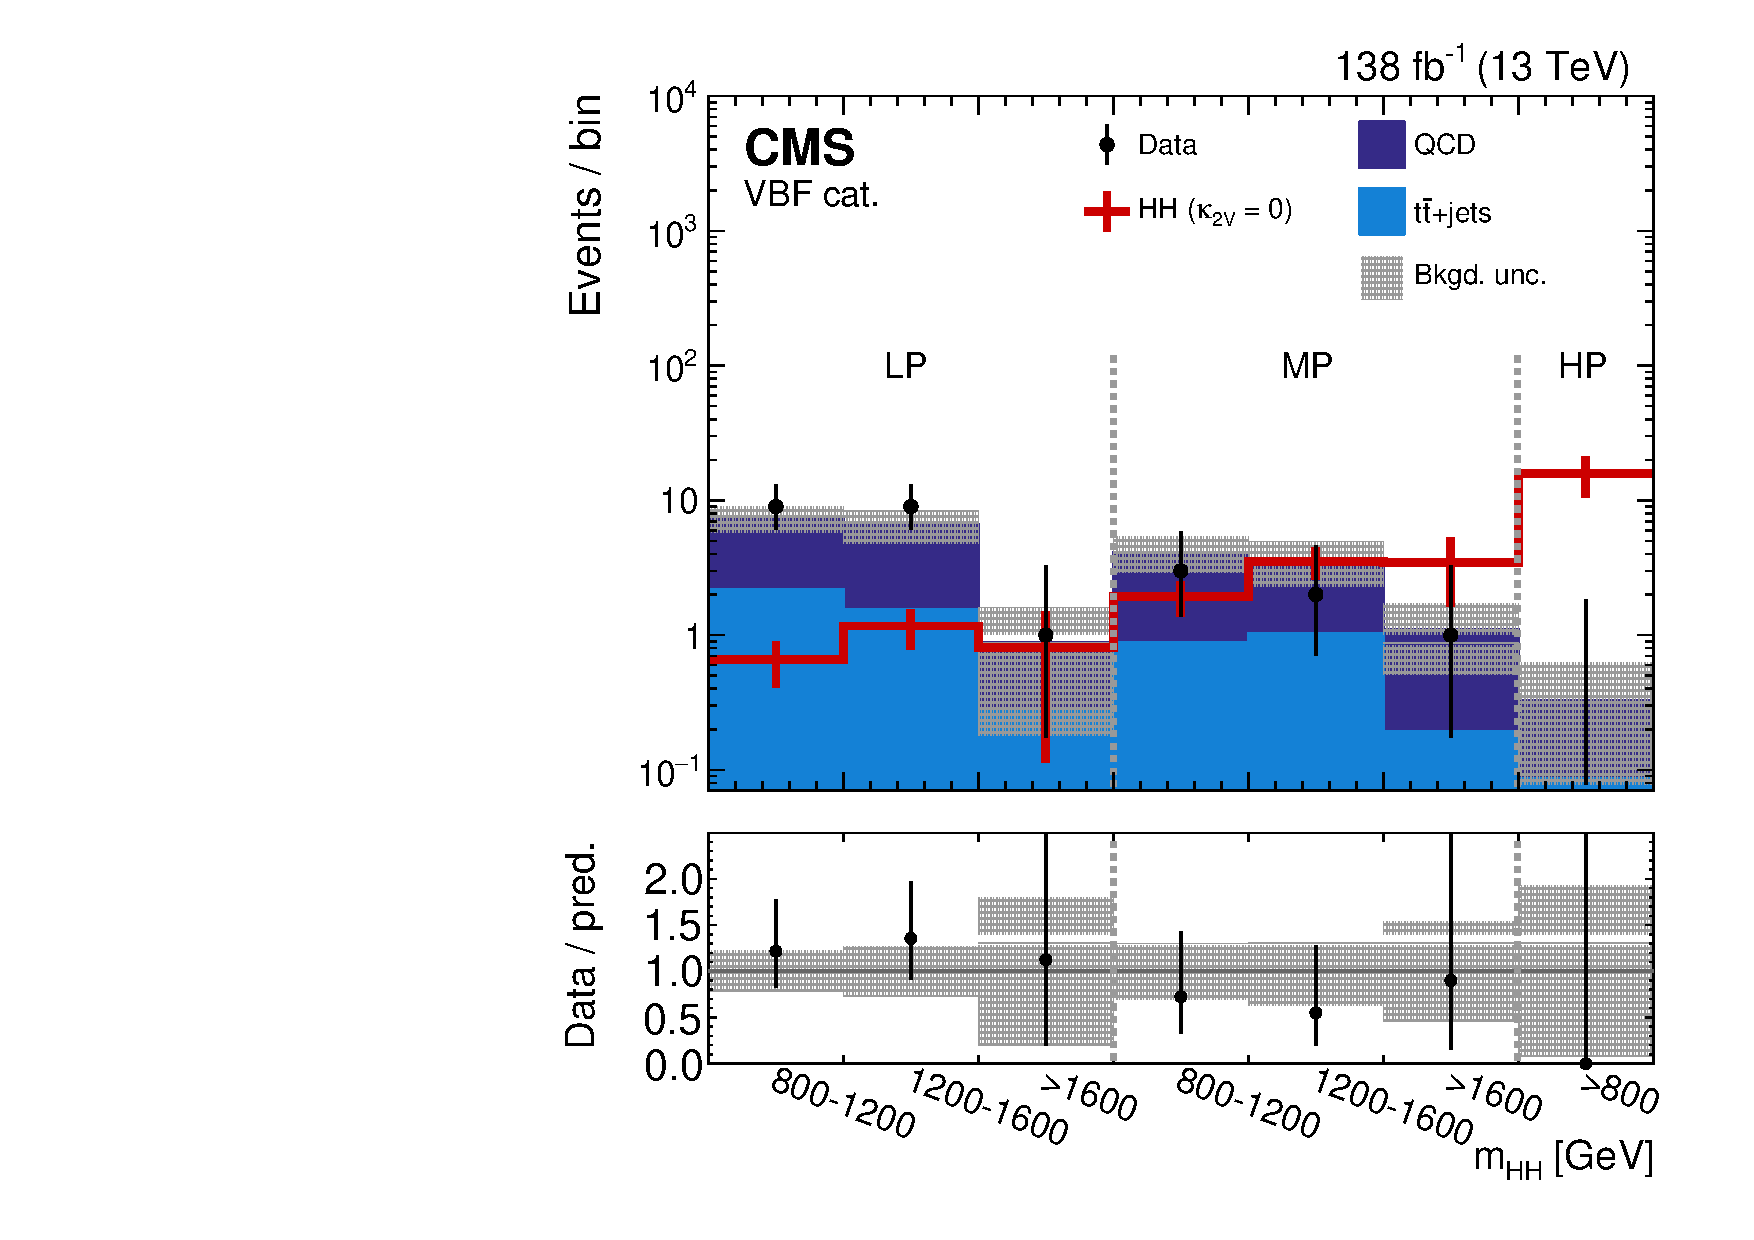
\includegraphics[width=0.33\textwidth]{figures/05-HH/CMS-results/4b/CMS-B2G-22-003_Figure_002.pdf}
    \caption[Distribution of events in the high-\mHH ggF category of the Run 2 CMS $\HH\to\bbbb$ resolved analysis~\cite{CMS:2022cpr}.]{Distribution of events in the high-\mHH ggF category of the Run 2 CMS $\HH\to\bbbb$ resolved analysis~\cite{CMS:2022cpr} as a function of the BDT discriminant (left), and of the Run 2 boosted analysis'~\cite{CMS:2022gjd} most sensitive ggF category, as a function of the second-highest tagged \bbbar-jet's mass (middle), and VBF categories, as a function of \mHH (right).}
    \label{fig:05_bbbb_run2}
\end{figure}

\begin{figure}[htb!]
    \centering
    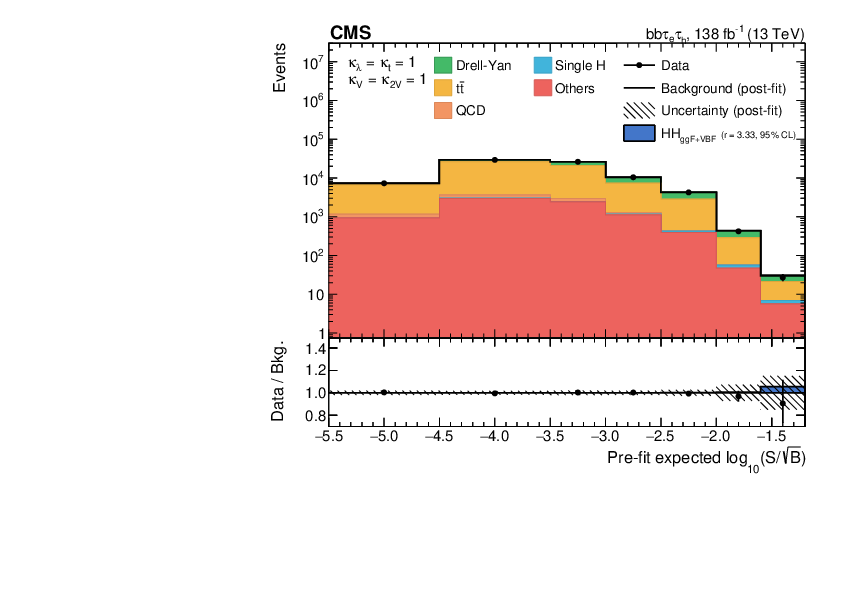
\includegraphics[trim=270pt 120pt 30pt 20pt, clip, width=0.32\textwidth]{figures/05-HH/CMS-results/bbtautau/Figure_005-a.png}
    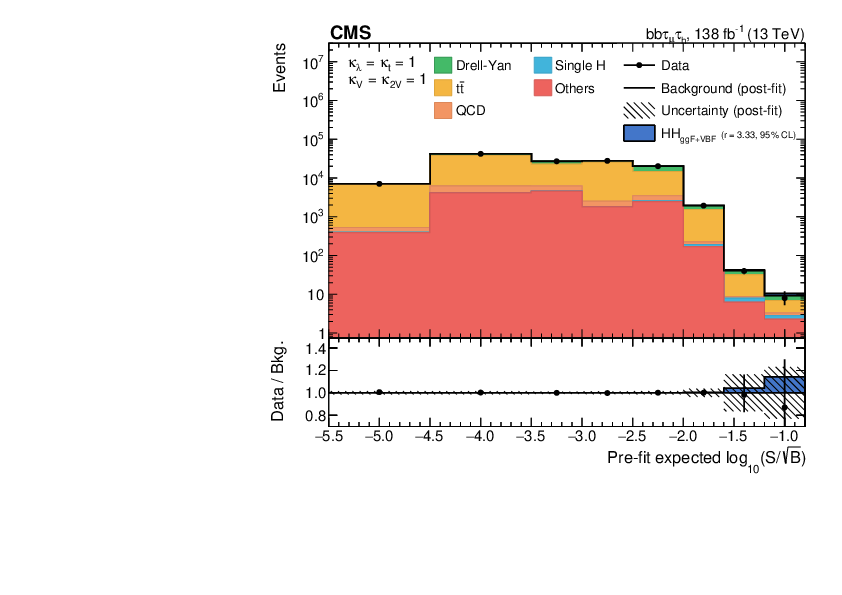
\includegraphics[trim=270pt 120pt 30pt 20pt, clip, width=0.32\textwidth]{figures/05-HH/CMS-results/bbtautau/Figure_005-b.png}
    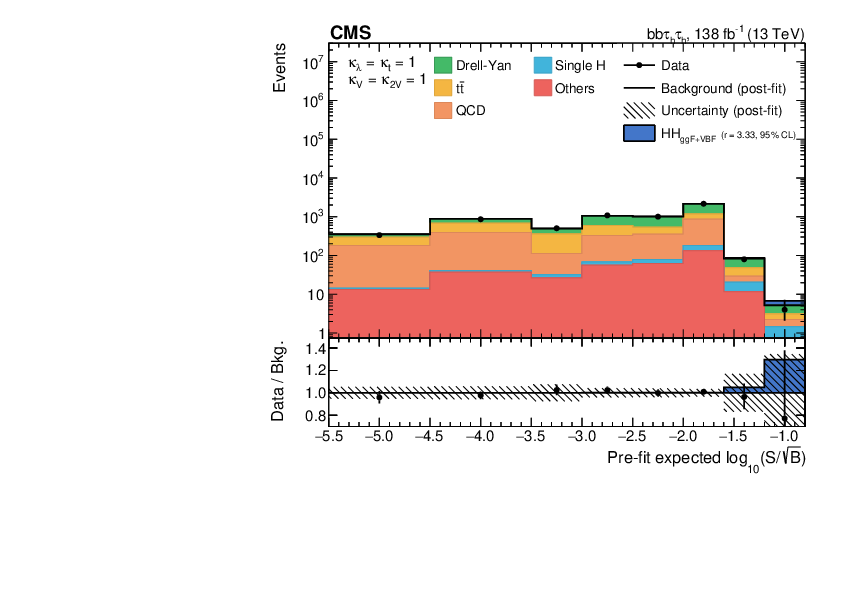
\includegraphics[trim=270pt 120pt 30pt 20pt, clip, width=0.32\textwidth]{figures/05-HH/CMS-results/bbtautau/Figure_005-c.png}
    \caption{Combination of bins of all postfit distributions of the Run 2 CMS $\HH\to\bbtautau$ analysis~\cite{CMS:2022hgz}, ordered according to the expected signal-to-square-root-background ratio, separately for the $\PGt_h\PGt_e$ (left), the $\PGt_h\PGt_\mu$ (center), and $\PGt_h\PGt_h$ (right) channels.}
    \label{fig:05_bbtautau}
\end{figure}

\begin{figure}[htb!]
    \centering
    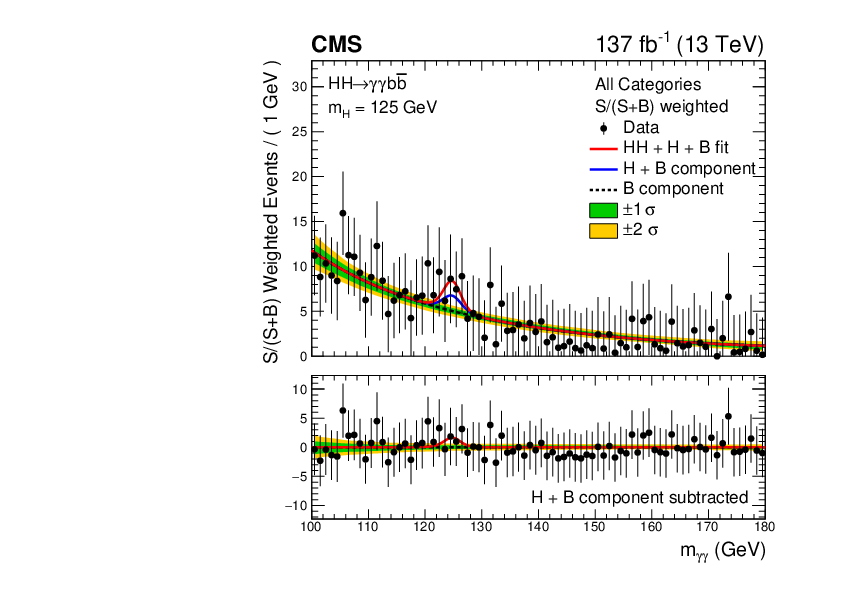
\includegraphics[trim=250pt 25pt 0 20pt, clip, width=0.5\textwidth]{figures/05-HH/CMS-results/bbgg.png}
    \caption[Invariant two-photon mass distribution of the Run 2 CMS $\HH\to\bbgg$ analysis~\cite{CMS:2020tkr}.]{Invariant two-photon mass distribution of the Run 2 CMS $\HH\to\bbgg$ analysis~\cite{CMS:2020tkr}, combined for all signal categories, weighted by S/(S+B), where S (B) is the number of signal (background) events extracted from the signal-plus-background fit.}
    \label{fig:05_bbgg}
\end{figure}

\begin{figure}[htb!]
    \centering
    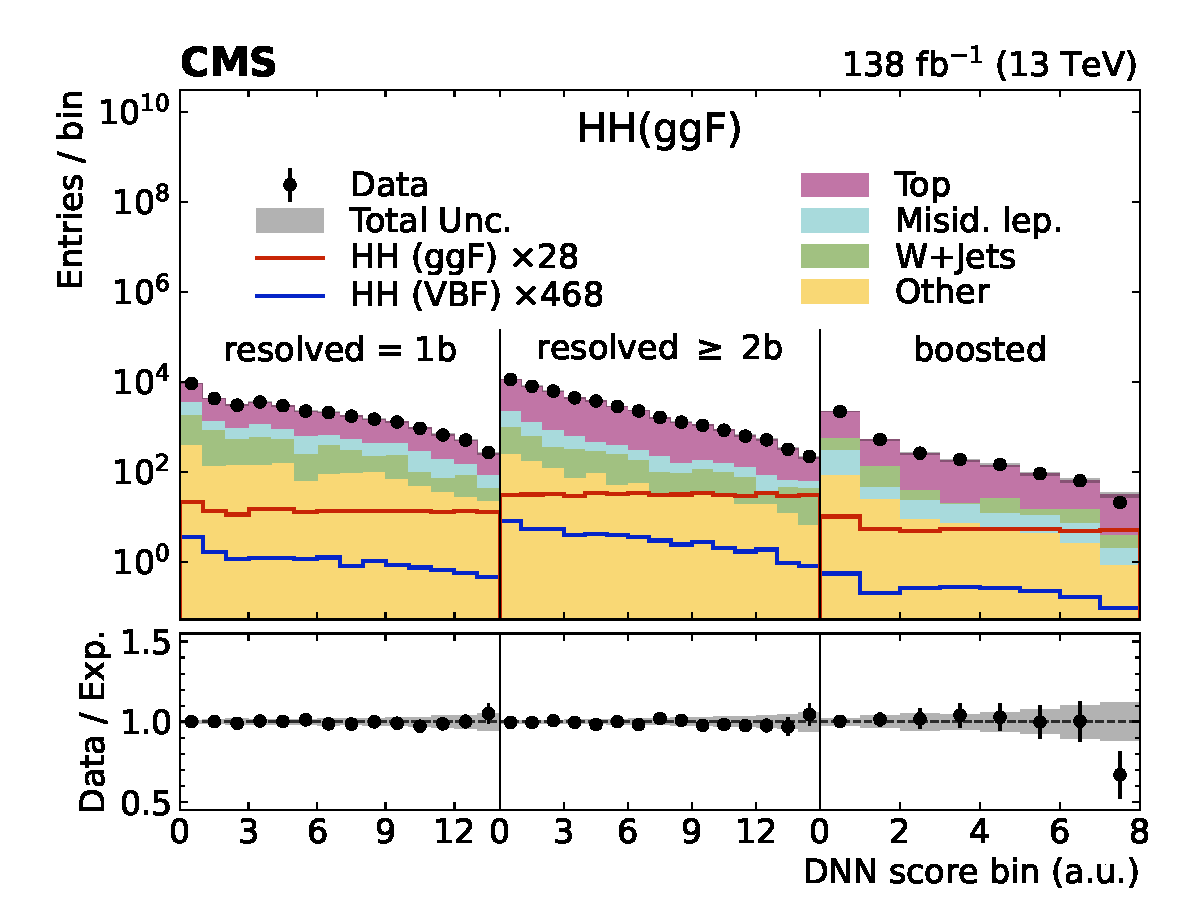
\includegraphics[width=0.49\textwidth]{figures/05-HH/CMS-results/bbww/CMS-HIG-21-005_Figure_005-a.pdf}
    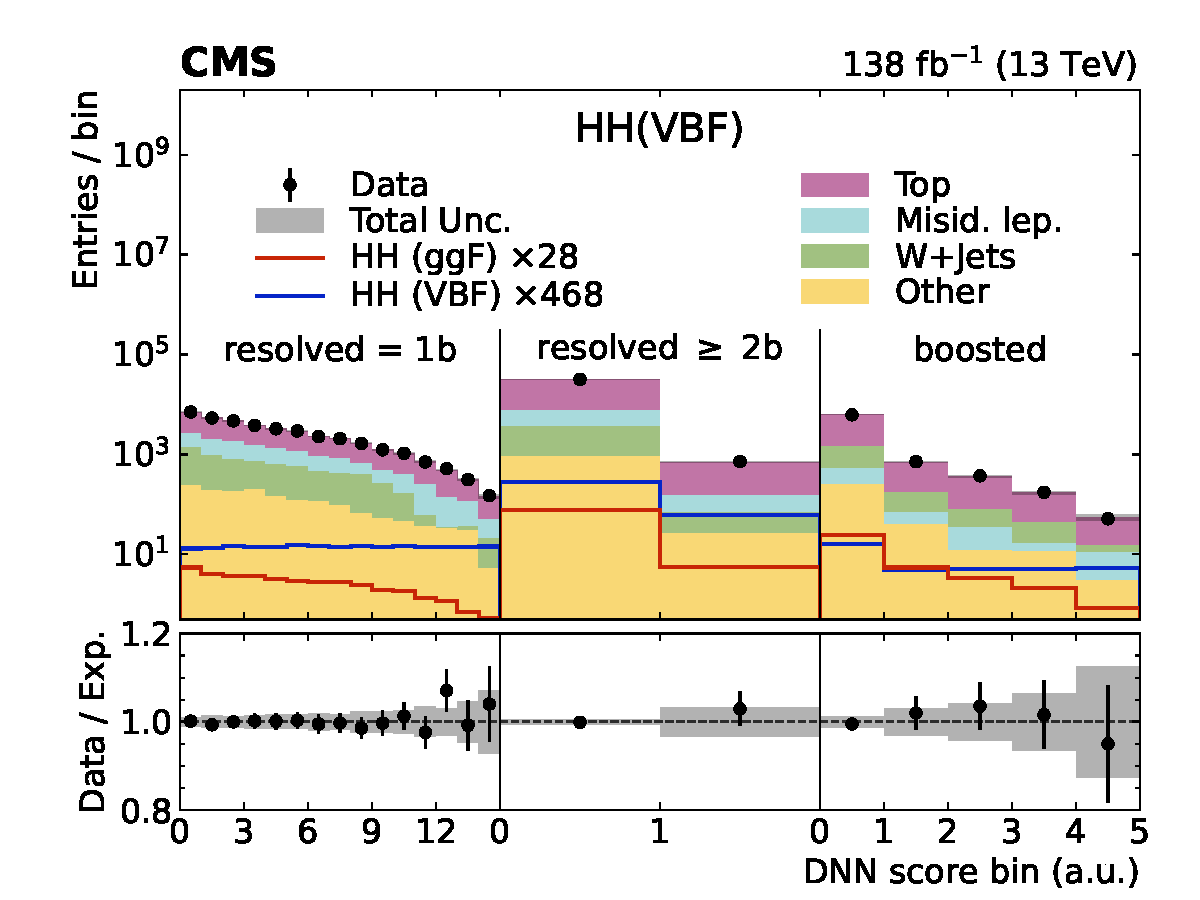
\includegraphics[width=0.49\textwidth]{figures/05-HH/CMS-results/bbww/CMS-HIG-21-005_Figure_005-b.pdf}
    \caption[Distribution of events in the resolved $1\Pb$, resolved $\geq2\Pb$, and boosted signal categories of the Run 2 CMS semi-leptonic $\HH\to\bbww$ analysis~\cite{CMS:2024rgy}.]{Distribution of events in the resolved $1\Pb$, resolved $\geq2\Pb$, and boosted signal categories of the Run 2 CMS semi-leptonic $\HH\to\bbww$ analysis~\cite{CMS:2024rgy} as a function of their DNN discriminant in the single-lepton (left) and double-lepton (right) final states.}
    \label{fig:05_bbww}
\end{figure}

The limits set on the \HH cross section by each channel, and their combinations, are shown in Figure~\ref{fig:05_hh_comb_xsec}, and as a function of \kapl and \kapvv in Figure~\ref{fig:05_hh_comb_kappa}.
The three ``golden channels'' each offer roughly similar sensitivities to the cross section and \kapl limits; however, the constraint on \kapvv is dominated by the boosted \bbbb channel, because of the enhancement of boosted \HH production at BSM \kapvv deviations, as discussed in Section~\ref{sec:05_smhh}.
Its observed (expected) $95\%$ confidence level (\CL) constraint is $[0.6, 1.4]$ ($[0.7, 1.4]$).
This is followed by the resolved \bbbb~\cite{CMS:2022cpr} and \bbtautau~\cite{CMS:2022hgz} channels, with constraints of $[-0.1, 2.2]$ ($[-0.4, 2.5]$) and $[-0.4, 2.6]$ ($[-0.6, 2.8]$), respectively.
Similarly, the strongest \kapvv constraint from the ATLAS experiment is from the recent boosted \bbbb search~\cite{ATLAS-CONF-2024-003}, with an observed (expected) $95\%$ \CL constraint of $[0.55, 1.49]$ ($[0.3, 1.7]$).

\begin{figure}[htb!]
    \centering
    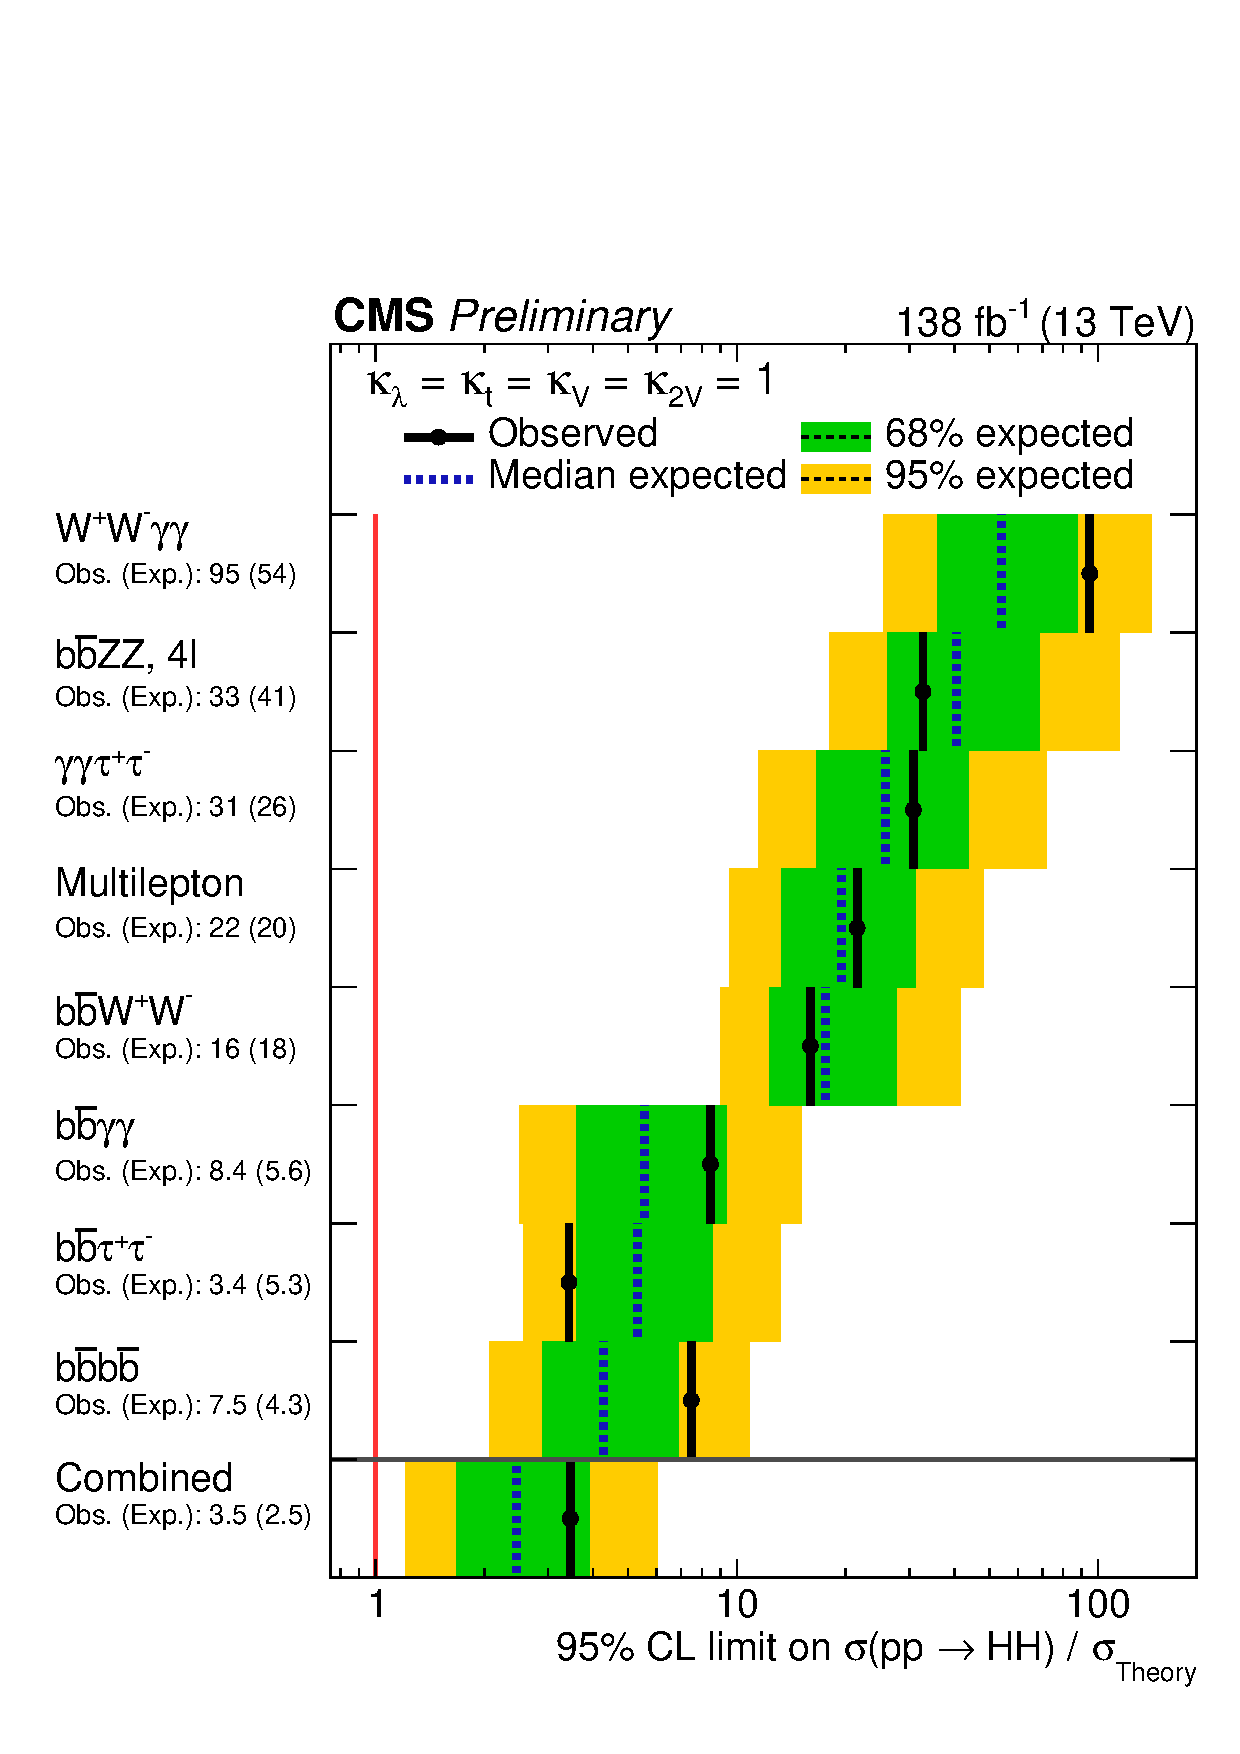
\includegraphics[width=0.8\textwidth]{figures/05-HH/CMS-results/HHcomb_xsec.pdf}
    \caption[The expected and observed limits on the ratio of experimentally estimated production cross section and the expectation from the SM in searches using different final states and their combination, reproduced from Ref.~\cite{CMS-PAS-HIG-20-011}.]{The expected and observed limits on the ratio of experimentally estimated production cross section and the expectation from the SM in searches using different final states and their combination, reproduced from Ref.~\cite{CMS-PAS-HIG-20-011}. 
    The search modes are ordered, from upper to lower, by their expected sensitivities from the least to the most sensitive. The overall combination of all searches is shown by the lowest entry.}
    \label{fig:05_hh_comb_xsec}
\end{figure}

\begin{figure}[htb!]
    \centering
    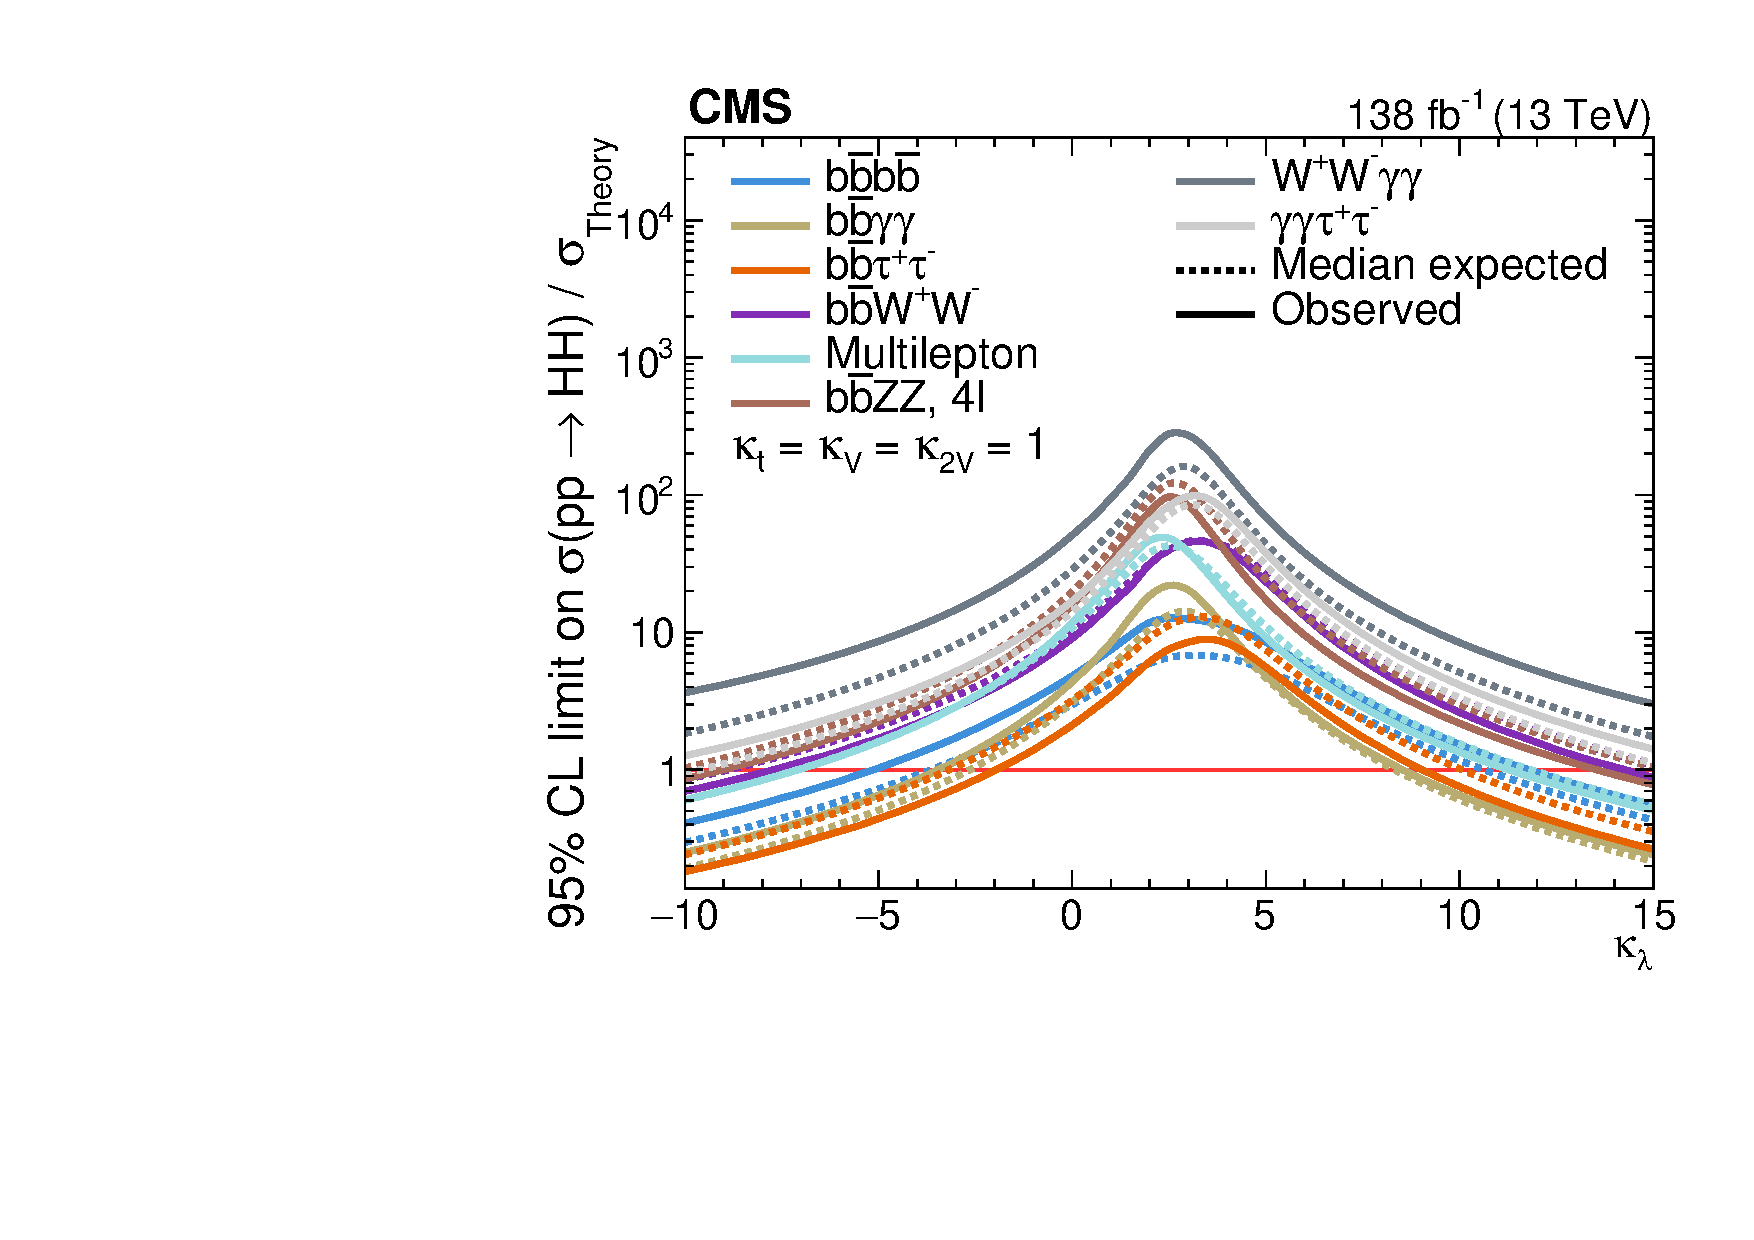
\includegraphics[width=0.49\textwidth]{figures/05-HH/CMS-results/kl_limits_channels_r_paper.pdf}
    \includegraphics[width=0.49\textwidth]{figures/05-HH/CMS-results/C2V_limits_channels_rqqHH_paper.pdf}
    \caption[The expected and observed limits on the ratio of experimentally estimated production cross section and the theory expectation.]{The expected and observed limits on the ratio of experimentally estimated production cross section and the theory expectation for different values of \kapl (left) and \kapvv (right), reproduced from Ref.~\cite{CMS-PAS-HIG-20-011}.}
    \label{fig:05_hh_comb_kappa}
\end{figure}


In this dissertation, we present the first search for nonresonant \HH production in the \textit{all-hadronic \bbvv channel}, where one Higgs decays to two bottom quarks, while the other to two vector bosons (\VV) both decaying hadronically to the four quark (\qqqq) final state.
Both the \PW and \PZ bosons are considered for the latter decay and collectively referred to as \PV bosons.
The branching fractions for the \bbbar and \VV decays are $0.58$ and $0.25$ respectively, for a total branching fraction $\mathcal{B}(\HHbbVV) = 2  \cdot0.58\cdot 0.25 = 0.29$, which is the second-highest, behind only \bbbb. 
The all-hadronic final state in particular has a branching fraction of $0.13$. 
The analysis targets the boosted regime, which, as discussed above, has the two-fold advantage of 1) increasing sensitivity to \kapvv deviations and 2) exponentially reducing the dominant QCD multijet background.



\subsection{BSM \texorpdfstring{\XHY}{X→HY} production}
\label{sec:05_bsmxhy}

\begin{figure}[htb] %[ht]
    \centering
    % \captionsetup{justification=centering}
    \includegraphics[width=\textwidth]{figures/05-HH/production/xhy.png}
    \caption{\XHY production in the symmetric (left) and asymmetric (right) cases.}
    \label{fig:05_xhy_production}
\end{figure} 

Many theoretical models predict a richer scalar sector than that in the SM to address aesthetic and observational inconsistencies with the SM, such as the Higgs mass hierarchy problem and the baryon asymmetry discussed above.
These include two-Higgs doublet models (2HDM)~\cite{Branco:2011iw} that add an additional scalar doublet to the SM, such as the minimal supersymmetric extension of the SM (MSSM)~\cite{Craig:2013hca}, which predicts two neutral CP-even scalars (\PH, \Ph), one neutral CP-odd scalar (\PA), and two charged scalars ($\PH^\pm$), where one of the neutral CP-even scalars may be the discovered SM Higgs \PHsm.
The next-to-minimal supersymmetric extension of the SM (NMSSM)~\cite{Domingo:2022kfm} adds to this a complex scalar singlet, predicting two more CP-even ($\Ph_{\mathrm{s}}$) and CP-odd ($\Pa_{\mathrm{s}}$) neutral scalars.
Finally, the two-real-singlet-model (TRSM) predicts two additional CP-even scalar fields.
Depending on the kinematics, all these models allow for cascade decays of a heavier scalar to symmetric and asymmetric lighter scalars, such as $\PH\to\PHsm\PHsm$ and $\PH\to\Ph\PHsm$, respectively, as shown in Figure~\ref{fig:05_xhy_production}.

We search for this broad class of signals, looking for generic decays of the form \XHY, where \PX is the heavier and \PY the lighter scalar resonance, with \PH decaying to \bbbar and \PY to \VVq. 
Many models, such as the TRSM, predict branching ratios for the lighter scalar similar to or the same as the SM Higgs.
In this case, the \VV decay modes are dominant for $\my > 140\GeV$ (Figure~\ref{fig:01_sm_higgs_hbrs}) and, hence, the \hbb and \yvv will be the dominant final states for the \XHY signal.
Thus, the \bbvv channel represents the highest BF in these models.

There are several published and ongoing CMS searches for \XHY production in a variety of regimes and final states with the Run 2 dataset, such as the boosted~\cite{BoostedXHY4b} \bbbb final state, the symmetric-only $\bbbar\PW\PW$ semi-leptonic final state~\cite{CMS:2024rgy}, the resolved $\bbbar\PGg\PGg$~\cite{CMS:2023boe}, and the resolved $\bbbar\PGt\PGt$~\cite{CMS:2021yci} final state. 
This dissertation presents the first search in the \bbvv all-hadronic state, and the first in the \bbvv state for the asymmetric case, representing a significant increase in the covered phase space for \XHY searches.

The search comprises two distinct topologies depending on the ratio of the \PX and \PY masses: a highly-boosted fully-merged \yvv topology for $\mx \gg \my$, with both \VV bosons' decay products highly collimated into a single wide-radius jet; and a relatively less-boosted semi-merged topology, where the \VV bosons are well separated and each \vqq decay is reconstructed as its own wide-radius jet.
These two phases are illustrated in Figure~\ref{fig:05_xhy_fraction_3q4q}, showing the fraction of \yvv jets containing three or four generator-level quarks as a function of the \PX and \PY boson masses, with the transition occurring around $\mx \approx 10\my$.
This dissertation focuses on a search for the fully-merged topology only, i.e. for $\mx \gtrsim 10\my$, and is complementary to an ongoing CMS search in the semi-merged topology.
Thus, in terms of the analysis strategy and techniques, this search is similar to the boosted nonresonant \HH search in that they both target highly-boosted Higgs boson decays with single wide-radius jets for both \PH or \PY bosons.

\begin{figure}[htb] %[ht]
    \centering
    % \captionsetup{justification=centering}
    \includegraphics[width=0.8\textwidth]{figures/05-HH/production/fraction_3q4q.pdf}
    \caption{The fraction of \yvv jets containing three or four generator-level quarks for the resonant \XHYbbVV signal as a function of the \PX and \PY boson masses.}
    \label{fig:05_xhy_fraction_3q4q}
\end{figure} 


% As shown in Figure~\ref{fig:01_sm_higgs_production}, both couplings can be accessed at the LHC exclusively through Higgs pair production.
% This dissertation describes one such measurement by the CMS experiment in the \bbvv channel, which is particularly sensitive to BSM deviations of the \HHVV coupling.
% It also presents a search for a new heavy resonance decaying to two Higgs bosons in the same channel, as predicted by many BSM theories described in Chapter~\ref{sec:05_bsmxhy}.


\subsubsection{Acknowledgements}

Chapters~\ref{sec:05_smhh} and~\ref{sec:05_bsmxhy} are in part, currently being prepared for the publication of the material by the CMS collaboration.
The dissertation author was the primary investigator and author of these papers.


% \section{Beyond the Standard Model}

% \subsection{Gravity}

%  - Gravity not a renormalizable QFT, can be thought of as an EFT in powers of (E/Mpl), so will never see the effect \\
%  - Experimentally, almost no consequence, but still fun to think about (although the 15 orders of magnitude gap makes you wonder if we are like the Greeks ``reasoning'' about atoms) \\
%  - String theory --- strings instead of particles, graviton arises, benefits: reproduces GR, SM etc. in the low-energy limit, but lots of unsolved problems \\
%  - Loop quantum gravity --- quantize space-time, only 4D, but so far does not reproduce our theories, interesting cosmological tests (constraint on spacetime quantization) \\
%  - Asymptotic safety --- Don't need gravity to be renormalizable, as long as the coupling constants have UV-safe fixed points (?), progress recently (see Weinberg 2009 lecture on motivation) \\


% \subsection{Grand unification}

%  - ``Zoo'' of particle representations can all be unified into two representations of a larger group SU(5), or even just a single huge representation of SO(10) (similar to two SU(2)'s embedded into SO(3, 1) or SO(4)) \\
%  - Very aesthetically pleasing, but moreover, lots of physical insights: charge quantization, proton charge = electron charge, \\
%  - SO(10) only: anti- / righthanded-neutrino, all fermions are encoded in ``five-bit strings'' (Zee) (although this predicts as-yet-unobserved fermions) \\
%  - Can keep adding bits / increasing the group size to include the different generations as well \\

%  - Similar to theories of quantum gravity, the GUT scale is so high that any effects will not be observed within our lifetimes sadly \\
%  - e.g. proton decay

% \subsection{Dark energy}

%  - Experimental evidence \\
%  - Higgs seesaw mechanism \\

% \subsection{Neutrino masses}

%  - Experimental evidence \\
%  - Seesaw mechanism \\

% \subsection{Dark matter}

%  - Experimental evidence \\
%  - WIMP, axion, sterile neutrinos, etc. \\
%  - Connections to Higgs \\

% \subsection{Baryon asymmetry}

%  - Sakharov conditions \\
%  - Relation to Higgs \\

% \subsection{Hierarchy problem}

%  - Is it a problem? \\
%  - Solutions \\

% \subsection{The SM as an effective field theory}

% HH EFT \\



% \section{Summary}

% \part{Experimental Background}
% \label{part:epp}

% \chapter{The CERN Large Hadron Collider}
\label{sec:02_lhc}

The Large Hadron Collider (LHC) is a proton-proton collider located at CERN on the border of Switzerland and France (Figure~\ref{fig:02_lhc_geneva}).
It is the largest and highest energy particle accelerator in the world, with a circumference of 27.6\unit{km} and a center-of-mass (COM) energy of 13.6\unit{TeV}, reproducing energies in the universe $10^{-11}$ seconds after the Big Bang.

\begin{figure}[ht]
    \centering
    \includegraphics[width=\textwidth]{figures/02-CMS/lhc/lhc_geneva.jpg}
    \caption{Outline of the LHC overlaid on a satellite image of Switzerland and France.}
    \label{fig:02_lhc_geneva}
\end{figure}

The tunnel was initially built for the large electron-positron collider (LEP), which operated from 1989 to 2000.
Being point particles and not interacting with the strong force, electrons and positrons produce ``clean'' collisions (i.e., with low background) and can be simulated with relative ease; thus, LEP allowed high precision measurements of the electroweak sector of the standard model (SM), as discussed in Chapter~\ref{sec:01_sm}.
The drawback, however, is that due to the power loss from synchotron radiation, which scales as $\propto ($mass of the accelerated particle$)^{-4}$, their low mass limits the COM energy that can be attained with electron-positron colliders.

Protons, on the other hand, are composite particles and produce ``noisy'', high-multiplicity collisions, but are $2000\times$ more massive and, hence, can be accelerated to much higher energies.
% The $1000\times$ higher mass of protons allows for much higher energies.
This is why, from early on, the LEP tunnel had also been proposed as a site for a future \textit{hadron-hadron} collider, which could achieve an order-of-magnitude greater energy than the previous energy-frontier machine, the Fermilab Tevatron.
The LHC was eventually approved in 1994 and was built in collaboration with over 100 countries at CERN between 1998 and 2008.
It is primarily a proton-proton collider, designed with the goal of accelerating each proton to $7\TeV$, for a COM energy of $14\TeV$, to explore the \TeV energy scale for the first time.
It also, less frequently, collides heavy ions to study QCD and the quark-gluon plasma inside nuclei.

The collisions occur at four interaction points around the ring and are observed by a total of nine detectors: two large general-purpose detectors, CMS and ATLAS, two more specialized detectors, ALICE and LHCb, for heavy-ion- and b-physics, respectively, and five smaller scale experiments, TOTEM, LHCf, MoEDAL, FASER, and SHiP.
In this section, we describe the LHC accelerator in Section~\ref{sec:02_lhc_accelerator} and the overall number of collisions, quantified as ``integrated luminosity'', it has delivered and expects to deliver in Section~\ref{sec:02_lhc_luminosity}.

\section{The accelerator}
\label{sec:02_lhc_accelerator}

The overall LHC accelerator complex is shown in Figure~\ref{fig:02_lhc_accelerator}.
Protons are first extracted from a hydrogen gas bottle through a duoplasmatron ion source~\cite{wolf1995handbook} as a low energy beam of around 100\unit{keV}.
They are then accelerated through a series of ``injectors'' (Figure~\ref{fig:02_lhc_injectors}): first through a linear accelerator (LINAC) up to 50\MeV; then a proton synchotron booster (PSB) up to 1.4\GeV; the proton synchotron (PS) up to 26\GeV; and finally through the super proton synchotron (SPS) up to 450\GeV, after which the protons are transferred to the LHC ring.

\begin{figure}[ht]
    \centering
    \includegraphics[trim=0pt 80pt 0pt 150pt, width=\textwidth]{figures/02-CMS/lhc/LHC_overall.pdf}
    \caption{Diagram of the LHC accelerator complex adapted from Ref.~\cite{Mouche:1708847}, depicting the initial proton source (in red), LINAC, proton synchotron booster, PS, SPS, LHC, and the four main experiments: CMS, ATLAS, ALICE, and LHCb.}
    \label{fig:02_lhc_accelerator}
\end{figure}

\begin{figure}[ht]
    \centering
    \captionsetup{justification=centering}
    \includegraphics[width=\textwidth]{figures/02-CMS/lhc/lhc_injectors.jpg}
    \caption{Schematic of the LHC injectors, reproduced from Ref.~\cite{Bruning:2012zz}.}
    \label{fig:02_lhc_injectors}
\end{figure}

Unlike particle-antiparticle colliders, like the Tevatron, which can accelerate both beams in the same ring with the same magnet system, the proton-proton collisions at the LHC require opposite magnetic fields for the beams before their collision.
The benefit, of course, is the ease of producing protons compared to antiprotons, allowing for far higher luminosities.
Due to the small 3.7\unit{m} internal diameter of the existing LEP tunnel, it was not possible to install two separate rings for the two counter-rotating beams; instead, a twin-bore magnet design~\cite{Blewett:1971zzb} was chosen to accommodate both in the same ring (Figure~\ref{fig:02_lhc_twinbore}) with two separate vacuum chambers and superconducting coils.

A total of 1,232 such superconducting NbTi dipole magnets are installed around the ring to maintain the circular trajectory of the protons, as well as 392 quadrupole and higher multipole-order magnets to focus the beams.
The maximum beam momentum $p$ is limited by the bending radius ($\rho$) and the bending field strength ($B$) of the dipole magnets, as~\cite{Bruning:2012zz}:
\begin{equation}
    p [\GeV / c] = B [\unit{T}] \rho [\unit{m}] / 3.336.
\end{equation}
For the LHC tunnel, $\rho$ is $2.8\unit{km}$; hence, to achieve 7\TeV protons, the dipole magnets were designed to achieve a field strength of 8.33\unit{T} (requiring liquid helium cooling to a temperature of 1.9\unit{K} to maintain superconductivity).
However, due to imperfections in some magnets, the LHC initially operated at 3.5--4\TeV per beam in Run 1 (2010--2012), then 6.5\TeV in Run 2 (2015--2018), and currently 6.8\TeV in Run 3 (2022--2026).

\begin{figure}[ht]
    \centering
    \includegraphics[width=0.49\textwidth]{figures/02-CMS/lhc/dipole_crossection.png}
    \includegraphics[width=0.49\textwidth]{figures/02-CMS/lhc/magnet.png}
    \caption{Diagram of the cross-section of the twin-bore LHC dipole magnets (left) and an image of an actual LHC dipole magnet (right), reproduced from Ref.~\cite{Evans:2008zzb}.}
    \label{fig:02_lhc_twinbore}
\end{figure}

The LHC layout comprises eight arcs and eight $\sim 500\unit{m}$ long straight sections.
The two beams are diverted and collided in four of the straight sections, called ``interaction points'' (IPs), where the detectors are located (Figure~\ref{fig:02_lhc_octants}).
The other four straight sections are used for utilities, such as the beam dump and collimation systems.

\begin{figure}[ht!]
    \centering
    \includegraphics[width=\textwidth]{figures/02-CMS/lhc/lhc_octants.jpg}
    \caption{Schematic of the LHC layout showing the two proton beams in green and blue and its division into eight octants, reproduced from Ref.~\cite{Bruning:2012zz}.}
    \label{fig:02_lhc_octants}
\end{figure}

The protons are accelerated and collided in ``bunches'' of $10^{11}$ protons each, with a separation of 25\unit{ns} between bunches.
The greater the number of protons per bunch and frequency of bunches, the greater the total luminosity of the collider.
Each bunch is accelerated and phase-focused longitudinally by a series of 16 superconducting radiofrequency (RF) cavities into separate ``RF buckets''.
The RF-frequency of the cavities is 400\unit{MHz}, corresponding to a theoretical minimum spacing in time of 2.5\unit{ns} between RF buckets / bunches.
The LHC opts for the 10-bucket spacing of 25\unit{ns} to avoid ``parasitic'' collisions between bunches~\cite{Bruning:2012zz}.
With this spacing, the maximum number of bunches in the ring is 2808.


\section{Luminosity and timeline}
\label{sec:02_lhc_luminosity}

As discussed in Chapter~\ref{sec:01_qft}, the number of scattering events we expect is the product of the scattering cross section and the \textit{luminosity} ($L$) of the particle beams (Eq.~\ref{eq:01_qft_interactions_cross_section_luminosity}).
Cross sections are typically given in units of barn (b), where $1\unit{b} = 10^{-28}\unit{m}^2$, and thus the luminosity often in inverse barns (b$^{-1}$).
For a circular collider, the instantaneous luminosity is given by~\cite{Bruning:2012zz}:
\begin{equation}
    \label{eq:02_lhc_luminosity}
    L = \frac{N_1 N_2 n_b f_{\mathrm{rev}}}{A},
\end{equation}
where $N_1$ and $N_2$ are the number of protons in each bunch, $n_b$ is the number of bunches, $f_{\mathrm{rev}}$ is the revolution frequency of the beams, and $A$ is the effective beam overlap area at the interaction point.
This is why the LHC design aims to maximize the number of protons per bunch, the number of bunches, and the frequency of bunches, while focusing and aligning the beams as much as possible at the interaction point.
The instantaneous luminosity of pp collisions at the LHC has increased steadily from a peak of $2.1\times10^{32}$\unit{cm$^{-2}$s$^{-1}$} in 2010 to around $2.5\times10^{34}$\unit{cm$^{-2}$s$^{-1}$} in 2022--24~\cite{cmslumi2024}.
Higher luminosity also leads to a higher rate of simultaneous pp collisions during a single bunch crossing, called \textit{pileup}, which results in background noise to the detectors.
As shown in Figure~\ref{fig:02_lhc_pileup}, the average rate of pileup in CMS has ranged from $10$ in 2011 to around $57$ in 2024.

The total luminosity delivered by the LHC is the integral of the above over time, called the \textit{integrated luminosity}, and is shown in Figure~\ref{fig:02_lhc_luminosity} along with the projection up to 2041.\footnote{Note that this projection has not been updated to reflect the decision made in September 2024 to extend Run 3 up to 2026 and delay the start of Run 4 to 2030.}
So far, the LHC has delivered around 60\unit{fb$^{-1}$} of integrated luminosity at $7$ or $8\TeV$ COM to the CMS and ATLAS experiments in Run 1, 138\unit{fb$^{-1}$} at $13\TeV$ in Run 2, and is currently aiming for around 300\unit{fb$^{-1}$} at $13.6\TeV$ in Run 3.
After this, (tentatively) between 2026 and 2030, the LHC will undergo a significant upgrade aiming to deliver an order of magnitude more luminosity in Runs 4--6, between $5$--$7\times10^{34}$\unit{cm$^{-2}$s$^{-1}$} instantaneously, integrated to around 3000\unit{fb$^{-1}$}!
This is called the High-Luminosity LHC (HL-LHC) upgrade~\cite{HL-LHC} (see Figure~\ref{fig:02_lhc_plan}), and is expected to allow access to rare processes such as Higgs boson pair production; however, it also entails major accelerator, detector, and computational challenges to effectively deliver and exploit the increased luminosity.

\begin{figure}[ht!]
    \centering
    \includegraphics[width=\textwidth]{figures/02-CMS/lhc/pileup_allYears}
    \caption{Mean number of interactions per crossing (pileup) in CMS between 2011--2024, reproduced from Ref.~\cite{cmslumi2024}.}
    \label{fig:02_lhc_pileup}
\end{figure}


\begin{figure}[ht!]
    \centering
    \includegraphics[width=\textwidth]{figures/02-CMS/lhc/luminosity.png}
    \caption{Integrated luminosity delivered by the LHC so far and the projection up to 2041, reproduced from Ref.~\cite{lhclumi}.}
    \label{fig:02_lhc_luminosity}
\end{figure}

\begin{figure}[ht!]
    \centering
    \includegraphics[width=\textwidth]{figures/02-CMS/lhc/HL-LHC_October2024.pdf}
    \caption{The LHC / HL-LHC operation and upgrade plan, reproduced from Ref.~\cite{hllhcplan}.}
    \label{fig:02_lhc_plan}
\end{figure}

% \chapter{The CMS detector}
\label{sec:02_cms}

\section{Overview}

The experimental apparatus used in this dissertation is the Compact Muon Solenoid (CMS) detector (Figure~\ref{fig:02_cms_detector}), one of the two general-purpose detectors at the LHC.
It is uniquely characterized by its strong, superconducting 3.8\unit{T} solenoid magnet, around which are arranged several subdetectors to measure the properties of particles produced in collisions at the LHC.
% It comprises a superconducting 3.8\unit{T} solenoid magnet and several subdetectors to measure the properties of particles produced in proton-proton as well as, to a lesser extent, heavy-ion collisions at the LHC.
Inside the solenoid, it contains an all-silicon tracker, to measure the momenta of charged particles and identify the collision vertex, and lead-tungstate crystal electromagnetic and brass and scintillator hadronic calorimeters to measure the energy of particles interacting through the electromagnetic and strong forces, respectively.
Finally, outside the solenoid are gas-ionization detectors, interleaved with steel flux-return yoke plates, to track muons. 

\begin{figure}[ht]
    \centering
    \includegraphics[width=\textwidth]{figures/02-CMS/cms/cms_schematic.png}
    \caption{A cutaway view of the CMS detector showing the various subdetectors and the solenoid magnet, reproduced from Ref.~\cite{CMS:2023gfb}.}
    \label{fig:02_cms_detector}
\end{figure}

% \begin{figure}[ht]
%     \centering
%     \captionsetup{justification=centering}
%     \includegraphics[width=\textwidth]{figures/02-CMS/cms/cms_raghav}
%     \caption{Author of the dissertation in front of the CMS detector in 2019.}
%     \label{fig:02_cms_raghav}
% \end{figure}

The CMS detector design was strongly motivated by the potential for discovery of the Higgs boson as well as new physics at the \TeV energy scale.
Specifically, the original design requirements were~\cite{CMS:2008xjf}:
\begin{itemize}
    \item Strong muon identification and momentum resolution, as well as good charge determination below $p < 1\TeV$;
    \item High charged-particle momentum resolution and reconstruction efficiency;
    \item Efficient triggering and good offline reconstruction of $\tau$-leptons and $b$-jets;
    \item Strong and hermetic electromagnetic energy resolution for photons and electrons;
    \item Good missing transverse energy (MET) and jet mass resolutions.
\end{itemize}
In addition to the above, the detector also had to be robust against the high radiation environment and pileup at the LHC, as well as have a powerful online event selection system, called the \textit{trigger}, to reduce the high raw 40\unit{MHz} data rate to something manageable for offline storage and analysis.

To satisfy the latter, events of interest in CMS are selected using a two-tiered trigger system. 
The first level (L1) uses custom hardware processors and information from the calorimeters and muon detectors to select events at a rate of around 100\unit{kHz} within a fixed latency of 4\unit{\mus}~\cite{CMS:2020cmk}. 
The second level, known as the high-level trigger (HLT), consists of a farm of processors running a version of the full event reconstruction software optimized for fast processing and reduces the event rate to around 1\unit{kHz} before data storage~\cite{CMS:2016ngn}.
Both online and offline, the raw detector signals are processed and reconstructed first locally as hits in the individual subdetectors, then as tracks and calorimeter clusters, and finally as physics objects such as electrons, muons, jets, and missing energy using the particle-flow (PF) algorithm~\cite{CMS:2017yfk}.

As we describe below, the CMS detector was able and continues to meet these ambitious requirements.
The CMS collaboration not only discovered the Higgs boson in 2012~\cite{CMS:2012qbp}, but also has since performed a wide range of measurements of the Higgs sector and the SM as well as searches for diverse new physics, such as those described in this dissertation.

Looking ahead, however, the upcoming high-luminosity era of the LHC (Chapter~\ref{sec:02_lhc_luminosity}) will bring forth considerable new challenges to the detector, with significantly higher radiation levels, occupancies, and pileup.
To overcome them, nearly all CMS subdetectors will undergo a major upgrade after Run 3, known as the Phase-2 upgrade~\cite{CMS:2017lum}.
The L1 trigger latency will be increased from 4 to 12.5\mus and the rate from 100 to 750\unit{kHz}, with an HLT rate of up to 10\unit{kHz}, to cope with the increased data rates (as well as incorporate tracking information at L1 for the first time)~\cite{Yates:2021dxs}.

Along with this, the Phase-2 upgrade includes the addition of new timing layers and the high granularity endcap calorimeter (HGCAL), which is notable not only for its ambitious design, but also the computational challenges it poses in detector simulation and reconstruction.
These challenges are a major motivation for the work described in Part~\ref{part:ml4sim}, exploring machine learning innovations to accelerate these simulations in CMS.
% To cope with the increased data rates (as well as incorporate tracking information for the first time), the L1 trigger latency will also be increased from 4 to 12.5\mus and the rate from 100 to 750\unit{kHz}, with an HLT rate of up to 10\unit{kHz}~\cite{Yates:2021dxs}.

In this chapter, we first introduce general concepts behind particle detectors in Section~\ref{sec:02_cms_particles}, before describing the individual CMS detector components in Section~\ref{sec:02_cms_detectors}.
The detector reconstruction and performance, as well as the PF algorithm is then discussed in Section~\ref{sec:02_cms_reconstruction}.
We conclude with the Phase-2 upgrade of CMS in Section~\ref{sec:02_cms_phase2}, including the HGCAL in Section~\ref{sec:02_cms_hgcal}.

\subsubsection{Coordinate system}

The CMS detector uses a coordinate system illustrated in Figure~\ref{fig:02_cms_coords}, with the origin set at the interaction point within the detector. 
The $x$-axis is oriented toward the center of the LHC ring, the $y$-axis is perpendicular to the plane of the LHC ring, and the $z$-axis is parallel to the beamline.
The azimuthal angle $\phi$ is measured in the $x$-$y$ plane, relative to the $x$-axis and the polar angle $\theta$ in the $x$-$z$ plane, relative to the $z$-axis.
Typically, $\theta$ is converted to the pseudorapidity $\eta = -\ln \left[ \tan \left( \cnicefrac{\theta}{2} \right) \right]$, which has a more useful scale for describing high energy collisions, and the angular separation between two particles is quantified using the variable $\Delta R = \sqrt{ (\Delta \phi)^2 + (\Delta \eta)^2 }$.
Finally, the transverse component of vectors, such as the transverse momentum \pt, are defined as projections onto the $x$-$y$ plane.

\begin{figure}[ht]
    \centering
    \captionsetup{justification=centering}
    \includegraphics[width=0.9\textwidth]{figures/02-CMS/cms/coordinate.png}
    \caption{The conventional CMS coordinate system.}
    \label{fig:02_cms_coords}
\end{figure}

\section{Detecting particles}
\label{sec:02_cms_particles}

\subsection{Particle interactions with matter}
\label{sec:02_cms_interactions}

In Part~\ref{part:sm}, we discussed the interpretation of fundamental particles as irreps of the Poincar\'e group and quantum excitations of fields.
In experimental physics, we have yet another interpretation: ``a particle is an object that interacts with your detector such that you can follow its track'' (W. Riegler~\cite{Riegler2013}).

Which is to say, in order to detect particles, they must interact with the detector material and transfer energy in a way that we can measure.
Out of the myriad particles produced in LHC proton-proton collisions, the are only eight particles stable enough to reach the CMS detector and be detected are listed in Table~\ref{tab:02_cms_particles}.
% are only nine particles stable enough to reach the CMS detector: photons, protons, neutrons, electrons, muons, charged pions, charged kaons, neutral kaons, and neutrinos.
Neutrinos are also stable, but are too weakly interacting to measure with the CMS detector, which means it is vital to measure the energy of all the other particles hermetically; the presence of neutrinos can then be inferred by energy conservation, or ``missing energy'' carried by neutrinos.

\begin{table}[ht!]
    \centering
    % \captionsetup{justification=centering}
    \caption{Particles which can reach and be detected by the CMS detector. Lifetimes are given in the rest frame for unstable particles.}
    \label{tab:02_cms_particles}
    \begin{tabular}{@{}lccc@{}}
        \toprule
        \textbf{Particle} & \textbf{Mass (MeV/$c^2$)} & \textbf{Charge ($e$)} & \textbf{Lifetime (s)} \\
        \midrule
        Photons                      & $0$                    & $0$     & Stable \\
        Electrons / positrons         & $0.511$                & $\pm1$    & Stable \\
        Protons                      & $938$                  & $+1$    & Stable \\
        Neutrons                    & $940$                 & $0$     & $880$ \\
        (Anti-)Muons                       & $106$                  & $\pm1$    & $2.2 \times 10^{-6}$ \\
        Charged pions                & $140$                  & $\pm1$  & $2.6 \times 10^{-8}$ \\
        Neutral kaons               & $498$                 & $0$                     & $9 \times 10^{-11}$---$5 \times 10^{-8}$ \\
        Charged kaons                & $494$                  & $\pm1$  & $1.2 \times 10^{-8}$ \\
        \bottomrule
    \end{tabular}
\end{table}

\subsubsection{Charged particles}

Out of these eight, the charged particles can interact electromagnetically with matter through:
\begin{itemize}
    \item Ionization and excitation of atoms: inelastic scattering with atomic electrons and elastic scattering from nuclei, respectively.
    The average energy loss per distance $\left\langle \cnicefrac{dE}{dx}\right\rangle$ of a particle due to ionization is given by the famous Bethe-Bloch formula~\cite{bethe1953passage}.
    \item Bremsstrahlung: photon radiation because of (de-)acceleration in the electric field of nuclei;
    \item Cherenkov effect: photon radiation due to the particle moving faster than the speed of light in the medium;
    \item and transition radiation: photon radiation due to the crossing a boundary between two different dielectrics.
\end{itemize}
Generally, for ``heavy'' charged particles (of mass $\gg$ electron mass), electromagnetic interactions are dominated by ionization and excitation, while for electrons and positrons, Bremsstrahlung is dominant at higher energies.
% The trajectories of low energy electrons and positrons can also deviate significantly due to \textit{multiple scattering} in the material.

The presence and angle of Cherenkov radiation depends on the particle momenta, a fact which is often exploited for ``particle identification'' (PID) by distinguishing particles of different masses at given momenta.
For example, LHCb uses ring-imaging Cherenkov (RICH) detectors to distinguish hadrons, which is critical for $b$-physics~\cite{LHCb:2008vvz}.
CMS, on the other hand, did not prioritize PID and cannot accurately distinguish between the different hadrons beyond their charge.

% accurately distinguish only between charged and neutral hadrons.

\subsubsection{Photons}

Photons primarily interact through:
\begin{itemize}
    \item The photoelectric effect: absorption by an atom causing the ejection of an electron, dominant at low energies, $\ll 1\MeV$;
    \item Compton scattering: incoherent scattering off an atomic electron, dominant at intermediate energies, $\sim 1\MeV$;
    \item and pair production: converting into electron-positron pairs in the Coulomb field of nuclei, dominant at high energies, $\gg 1\MeV$.
\end{itemize}
The combination of these effects means that as high energy electrons and photons propagate through the detector material, they produce a cascade of secondary particles, called an \textit{electromagnetic shower}, which are analyzed to infer the presence and overall energy of the originating particle.

It is often convenient to characterize detector materials by their \textit{radiation length} ($X_0$), which is the mean distance into the material over which high-energy electrons lose $\cnicefrac{1}{e}$ of their energy due to Bremsstrahlung, and $\cnicefrac{7}{9}$ of the mean free path of photons before pair production.

\subsubsection{Hadrons}

Finally, high energy hadrons can also interact with atomic nuclei through the strong force, losing energy through further particle emissions which create their own \textit{hadronic shower}.
As a large fraction of these emitted particles are neutral pions, which decay immediately into photons, hadronic showers are also often accompanied by electromagnetic sub-showers.
We can characterize materials for hadron detection similarly by their \textit{nuclear interaction length} ($\lambda$), the mean free path between nuclear interactions.

\subsection{Types of detectors}
\label{sec:02_cms_detecting_detectors}

\subsubsection{Tracking detectors}

The earliest particle detectors were gaseous \textit{ionization chambers}.
Charged particles passing through these detectors ionize the gas along their trajectory, creating visible tracks, which can be captured, for example, by using an electric field to push the ions towards photographic film.
The most notable examples are cloud chambers, which were prominent in the first half of the 20th century, and led to the discovery of the positron, muon, and kaon via cosmic rays.
The Nobel Prize was awarded to Charles Wilson in 1927 and Carl Anderson in 1936 for the invention and development of the cloud chamber, respectively.

% for the invention of the cloud chamber, and to Carl Anderson in 1936 for the discovery of the positron.
% Charles Wilson and Carl Anderson were awarded the Nobel Prize in 1927.
% as well as Nobel prizes for their inventors.

Tracking detectors have since continuously evolved, such as through the use of liquid media in \textit{bubble chambers} and charged wires to produce electric fields and read out ionization signals electronically in \textit{wire chambers}, both of which again led to Nobel Prizes for their inventors, Donald Glaser and Georges Charpak, respectively.
% Both inventions again led to Nobel Prizes, for Donald Glaser in 1960 and Georges Charpak in 1992, respectively.
The Gargamelle bubble chamber at CERN notably led to the discovery of weak neutral currents~\cite{GargamelleNeutrino:1973jyy} (see Chapter~\ref{sec:01_sm_ew_weak}).

More recently, a significant advancement in tracking detectors has been achieved through the use of semiconductors such as silicon.
A $p$-$n$ semiconductor diode~\cite{sparkes1994semiconductor, Nomerotski:2009zz} effectively forms an ionization chamber as well, where charged particles passing through will create electron-hole pairs whose charge can be collected and recorded.
Semiconductor detectors can have lower ionization energies, higher granularity, better position and time resolution, and strong radiation tolerance, while also being able to leverage innovations and state-of-the-art fabrication techniques from the semiconductor industry.

Thus, there has been a gradual shift towards their use, particularly in collider physics.
Here, tracking detectors are crucial for (1) \textit{vertexing} --- measuring particle tracks precisely to determine the point of collision, or the ``vertex'' --- and (2) measuring the curvature of charged-particle trajectories in a magnetic field to determine their momenta.
Silicon trackers, for example, were employed for vertexing in all LEP experiments and the CDF and D\O experiments at the Tevatron.
The CMS detector is notably the first to use silicon for its entire tracking volume.

Semiconductor trackers are, however, more expensive per unit area.
Hence, gaseous and liquid detectors remain prevalent in particle physics, particularly where large volumes are required, such as in neutrino experiments and the CMS muon system.

\subsubsection{Calorimeters}

Calorimeters are detectors designed primarily to measure the energy of particles.
They can be either \textit{homogeneous}, where the entire volume of the detector can both absorb \textit{and} measure the energy of the shower; or, \textit{sampling}, where separate ``passive'' layers which absorb energy and initiate the shower are interleaved with ``active'' layers to measure the energy.
Sampling calorimeters are less precise than homogeneous calorimeters, but are more cost-effective, especially when large volumes are required.
CMS employs both types of calorimeters, and primarily uses \textit{scintillation} --- photon emission due to atomic (de-)excitation from charged particles --- to capture and measure energy.

Generally in collider physics trackers are designed to have short radiation lengths, to minimize particle energy loss, and calorimeters as long a radiation length as possible, to capture the entire energy of electromagnetic or hadronic showers.
In addition to their radiation and nuclear interaction lengths, calorimeter materials are characterized as well by their \textit{Moli\`ere radius} ($R_M$), which is the radius of a cylinder containing, on average, 90\% of an incident electron or photon's electromagnetic shower energy.
It is approximately related to $X_0$ as:
\begin{equation}
    \label{eq:02_cms_moliere}
    R_M = 0.0265 X_0 (Z + 1.2),
\end{equation}
where $Z$ is the atomic number of the material.

\subsubsection{General-purpose detectors}

Designing a general-purpose detector, such as CMS, requires a careful optimization of several factors, including high efficiency and resolution for as many of the particles in Table~\ref{tab:02_cms_particles}, radiation hardness, cost effectiveness, and more.
A typical compromise in particle physics has been a ``layered'' detector design, as shown in Figure~\ref{fig:02_cms_layers}, with a thin (in radiation and nuclear interaction lengths) innermost tracker for precise vertexing and momentum measurements, followed by thick calorimeters to measure particle energies, and finally dedicated detectors to identify and measure high energy muons that are able to penetrate the previous layers.
The CMS detector follows this general philosophy, as shown in Figure~\ref{fig:02_cms_slice}.

\begin{figure}[ht]
    \centering
    \includegraphics[width=\textwidth]{figures/02-CMS/cms/interactions_layers_edit2.pdf}
    \caption{Layers in a typical general-purpose detector in particle physics and an illustration of the interactions of different particles.}
    \label{fig:02_cms_layers}
\end{figure}

\begin{figure}[ht!]
    \centering
    \includegraphics[width=\textwidth]{figures/02-CMS/cms/components/slice.png}
    \caption{Illustration of the different detector layers in the CMS barrel region and the expected hits and energy deposits from various particles, reproduced from Ref.~\cite{Davis:2205172}.}
    \label{fig:02_cms_slice}
\end{figure}

\section{CMS detector components}
\label{sec:02_cms_detectors}

\subsection{The magnet}
\label{sec:02_cms_magnet}

The defining characteristic of the CMS detector is its strong $3.8\unit{T}$ solenoid magnet, with a $11.4 \unit{T\,m}$ bending power (Figure~\ref{fig:02_cms_magnet}).
% , which allows precise measurements of charged-particle momenta in the tracker.
Its large $6\unit{m}$ diameter and $13\unit{m}$ length accommodate not only the tracker for momentum measurements, but also the calorimeters in order to reduce the material in front of them.
The strength of the magnet was chosen to allow precision measurements of charged-particle momenta and to achieve a target \pt resolution of 10\% for 1\TeV muons.

\begin{figure}[ht]
    \centering
    \includegraphics[width=\textwidth]{figures/02-CMS/cms/components/magnet_lowering.jpg}
    \caption{The CMS solenoid, as it was being lowered into the CMS cavern in 2007, reproduced from Ref.~\cite{Maximilien:1020310}.}
    \label{fig:02_cms_magnet}
\end{figure}

As shown in Figures~\ref{fig:02_cms_detector} and~\ref{fig:02_cms_slice} in red, the solenoid is additionally surrounded by massive layers of steel ``return yoke'', weighing 12,000 tonnes in total, for several complementary reasons:
(1) it confines the magnetic field, improving the efficiency and safety of the detector, by providing a low-reluctance path for the magnetic field lines to return to the solenoid; 
(2) it is interleaved with the CMS muon system and provides a residual magnetic field for muon tracking; 
(3) it absorbs the remaining particles not been completely contained by the calorimeters; 
and, finally, (4) it provides structural support to the detector.
The resulting magnetic field throughout CMS is shown in Figure~\ref{fig:02_cms_magnetic_field}, where we can see a uniform $3.8\unit{T}$ field within the solenoid and an $\approx 2\unit{T}$ field in the return yoke.

\begin{figure}[ht]
    \centering
    \includegraphics[width=\textwidth]{figures/02-CMS/cms/components/magnetic_field}
    \caption{Measurement using cosmic rays (left) and illustration (right) of the CMS magnetic field, reproduced from Ref.~\cite{CMS:2009moq}.}
    \label{fig:02_cms_magnetic_field}
\end{figure}

\subsection{Tracker}
\label{sec:02_cms_tracker}

\begin{figure}[ht]
    \centering
    \includegraphics[width=\textwidth]{figures/02-CMS/cms/components/Phase1_Tracker_1Quarter.pdf}
    \caption{Schematic of one quarter of the Phase-1 CMS tracker in the $r$-$z$ plane, reproduced from Ref.~\cite{CMS:2017lum}.
    In green are the pixel detector layers, in red the single-sided strip modules, and in blue the double-sided strip modules.}
    \label{fig:02_cms_tracker}
\end{figure}

The CMS tracker is designed to achieve the key detector requirements of strong charged-particle momentum resolution and efficient online and offline $\tau$ and $b$-jet reconstruction.
It must additionally operate at a high efficiency at the expected average pileup rate of 20-60 collisions per bunch crossing in Runs 1--3 of the LHC.
To do so, as illustrated in Figure~\ref{fig:02_cms_tracker}, it comprises relatively small and granular silicon \textit{pixel} layers close to the interaction point for precise vertexing, followed by larger silicon \textit{strip} layers.
The tracker has an overall diameter of 2.5m and length of 5.8m, and is composed of a separate co-axial ``barrel'' region and two ``endcap'' regions perpendicular to the beamline, to provide pseudorapidity coverage of $\abs{\eta} \lesssim 2.4$.

Silicon has several advantages for tracking detectors: it can be made radiation hard to be placed close to the interaction point~\cite{BaselgaBacardit:2015iqn}; it has a low ionization energy of $3.6$\unit{eV}; it can be made thin --- the maximum radiation and nuclear interaction lengths over the entire CMS tracker are around $2$ and $0.6$ respectively (Figure~\ref{fig:02_cms_tracker_material}); it is naturally abundant and widely used in the semiconductor industry; and it can be easily patterned to small dimensions for high granularity.
This is why, as discussed in Section~\ref{sec:02_cms_detectors}, silicon has gained popularity in particle physics, with CMS being the first to use it for the entire tracker.
% Because of these benefits, silicon has gradually gained prominence for particle tracking, being employed for vertexing in all LEP experiments and the CDF and D0 experiments at the Tevatron.
% The CMS detector was the first to use silicon for the entire tracker.

\begin{figure}
    \centering
    \includegraphics[width=0.49\textwidth]{figures/02-CMS/cms/components/figs_2011_cmsTracker_MaterialBudget_InteractionLengths.png}
    \includegraphics[width=0.49\textwidth]{figures/02-CMS/cms/components/figs_2011_cmsTracker_MaterialBudget_RadLengths.png}
    \caption[Total thickness $t$ of the tracker material traversed by a particle produced at the nominal interaction point.]{Total thickness $t$ of the tracker material traversed by a particle produced at the nominal interaction point, as a function of pseudorapidity $\eta$, expressed in units of radiation length $X_0$ (left) and nuclear interaction length $\lambda_I$ (right), reproduced from Ref.~\cite{CMS:2014pgm}.}
    \label{fig:02_cms_tracker_material}
\end{figure}

The pixel tracker includes three barrel layers at radii of 4.4, 7.3, and 10.2\unit{cm} and two pairs of endcap disks at $z = \pm34.5$ and $\pm46.5\unit{cm}$. 
It contains a total of 1440 modules and 66 million pixels, of size (or ``pitch'') $100\times150$\unit{$\mu$m$^2$}, and thickness $285$\unit{$\mu$m}.
The planar position of the sensor provides a third position coordinate as well.
The pixel tracker yields an overall hit position resolution of $10$--$20$\unit{$\mu$m} in the transverse direction --- $r\phi$ in the barrel ---  and $20$--$40$\unit{$\mu$m} in the longitudinal direction --- $z$ in the barrel.
The pixel orientation is optimized most for $r\phi$ resolution, as that is the plane in which charged particles bend from the CMS magnetic field.

Silicon strip modules are longer than pixels, providing high granularity only in one axis, but are more cost-effective; hence, they are used in the outer layers of the CMS tracker, which require a much larger area of coverage: $198$\unit{m$^2$} of active coverage versus $1.1$\unit{m$^2$} for the pixels.
The strip tracker has 10 barrel layers and three small and nine large endcap disks, with a total of 15,148 modules and 9.3 million strips.
It contains two types of strip modules: standard ``single-sided'' modules as well as ``double-sided`` modules mounted back-to-back at a stereo angle to effectively allow pixel-like 2D measurements as well, albeit at a lower granularity.

The strip modules in the barrel are aligned parallel to the beamline with a pitch ranging from $80$--$183$\unit{$\mu$m}, while those in the endcaps are mounted in the radial direction with a pitch of $81$--$205$\unit{$\mu$m}.
Overall, the strips in the inner barrel and disk layers provide an $r\phi$ resolution of $13$--$38$\unit{$\mu$m}, while the outer layers provide $18$--$47$\unit{$\mu$m}.


\subsection{ECAL}

The CMS electromagnetic calorimeter (ECAL) (Figure~\ref{fig:02_cms_ecal}) was designed to precisely measure energies of electrons and photons.
It was particularly optimized for sensitivity to the Higgs-to-two-photon decay channel, which proved crucial to the discovery of the Higgs boson~\cite{CMS:2012qbp}.
% It was especially optimized for high sensitivity to the Higgs to two photon decay channel, which proved crucial to the discovery of the Higgs boson.

The ECAL is a homogeneous calorimeter made out of 75,848 lead-tungstate (PbWO$_4$) crystals (Figure~\ref{fig:02_cms_ecal_crystals}), which are a type of highly transparent scintillators.
PbWO$_4$ was chosen for its high density (8.28\unit{g/cm$^3$}), short radiation length ($X_0 = 0.89\unit{cm}$), and small Moli\`ere radius ($R_M = 2.2\unit{cm}$), which allows for a compact calorimeter with fine granularity.
Additionally, its fast scintillation response ($\approx 10\unit{ns}$) allows distinguishing between ``out-of-time'' (OOT) pileup --- particles produced from adjacent bunch crossings --- and particles from the primary interaction~\cite{CMS:2020xlg}.
%  and the ability to minimize ambiguity between particles from different bunch crossings.
The scintillation light is detected by photodiodes glued to the back of each crystal.

\begin{figure}[ht]
    \centering
    \includegraphics[width=\textwidth]{figures/02-CMS/cms/components/ecal_layout.png}
    \caption{Layout of the CMS ECAL, reproduced from Ref.~\cite{Cooke:2022lbl}, with one of the 36 barrel regions highlighted in yellow, the preshower in pink, and the endcap regions in green.}
    \label{fig:02_cms_ecal}
\end{figure}

\begin{figure}[ht]
    \centering
    \captionsetup{justification=centering}
    \includegraphics[width=0.4\textwidth]{figures/02-CMS/cms/components/PbWO4_crystals.png}
    \caption{PbWO$_4$ crystals and photodiodes used in the CMS ECAL.}
    \label{fig:02_cms_ecal_crystals}
\end{figure}

Like the tracker, it has a barrel region, covering $\abs{\eta} < 1.48$, and two endcap regions for $1.48 < \abs{\eta} < 3.00$.
They have thicknesses of $25.8X_0$ and $24.7X_0$, respectively, and a total nuclear interaction length of around 1.
This is sufficient to contain >$98\%$ of the energy of $\leq 1\TeV$ electrons and photons, and causes around two thirds of charged hadrons to shower in the ECAL as well.

Additionally, the ECAL includes a ``Preshower'' sampling calorimeter in the endcap regions, which comprises two layers of $3X_0$ of lead to initiate electromagnetic showers, interleaved with active silicon strip detectors for measurements.
The purpose of the Preshower is primarily to distinguish between single photons and neutral pion decays into two, close-by, photons in the forward regions, whose energy deposits in the ECAL would otherwise overlap significantly.

\subsection{HCAL}

The CMS hadronic calorimeter (HCAL) sits roughly $30\unit{cm}$ outside the ECAL and is designed to measure the energies of neutral and charged hadrons.
It is composed of four major sections: the HCAL barrel (HB), the HCAL endcap (HE), the HCAL outer (HO), and the HCAL forward (HF) (Figure~\ref{fig:02_cms_hcal}).
Due to their much greater volume compared to the ECAL, the HB, HE, and HO are all chosen to be sampling calorimeters, with alternating layers of absorber material and plastic scintillator.
The HF extends the pseudorapidity coverage of CMS up to $\abs{\eta} = 5.2$ and is a steel and quartz-fiber \textit{Cherenkov calorimeter}.

The HB has 14 total layers of brass absorbers and scintillators, with additional steel front and back plates, covering $\abs{\eta} < 1.4$~\cite{CMS:2008xjf}.
Due to its radial constraints, with the ECAL and magnet on either side, it has a thickness at $\eta = 0$ of only $5.8\lambda$, with the ECAL adding another $\approx1\lambda$.

\begin{figure}[ht]
    \centering
    \includegraphics[width=\textwidth]{figures/02-CMS/cms/components/hcal_layout.png}
    \caption{Layout of the CMS detector in the $r$-$z$ plane with the four HCAL sections labeled, reproduced from Ref.~\cite{CMS:2012tda}.}
    \label{fig:02_cms_hcal}
\end{figure}

To capture the remaining ``tails'' of hadronic showers in the barrel region, the HO is placed outside the solenoid.
It uses the same scintillators and electronics as the HB, but uses the magnet and return yoke materials themselves as absorbers, adding up to $3\lambda$ more of material. 
Figure~\ref{fig:02_cms_hcal_ho} demonstrates that the HO is crucial for capturing the entire energy of hadronic showers: without it, we see an excess of events with the measured energy of hadrons lower than their incident energy, implying a loss of energy with the HB alone.

\begin{figure}[ht]
    \centering
    \includegraphics[width=0.7\textwidth]{figures/02-CMS/cms/components/hcal_ho_energy.png}
    \caption[Simulation of the distribution of measured $/$ incident energy for pions with incident energies of $200\GeV$ at $\eta = 0$, reproduced from Ref.~\cite{CMS:2008xjf}.]{Simulation of the distribution of measured $/$ incident energy for pions with incident energies of $200\GeV$ at $\eta = 0$, reproduced from Ref.~\cite{CMS:2008xjf}.
    Without the HO, there is an excess of events with the measured energy lower than the incident, while with the HO the distribution is a Gaussian centered at 1, implying recovery of the total pion shower energy.}
    \label{fig:02_cms_hcal_ho}
\end{figure}

The HE covers the pseudorapidity range $1.3 < \abs{\eta} < 3.0$ and has 18 layers of brass and scintillators, for a total length of $10\lambda$ including the ECAL.
The granularity of both the HB and HE for $\abs{\eta} < 1.6$ is $0.087\times0.087$ in $\eta$-$\phi$, while for $\abs{\eta} > 1.6$ in the HE it increases to $0.17\times0.17$.

The HF is placed 11.2\unit{m} from the interaction point to cover the very forward range $3.0 < \abs{\eta} < 5.2$.
Its primary design constraints are the extremely hostile radiation levels in the high-rapidity region, and hence uses steel absorbers and quartz fibers that are radiation hard~\cite{Penzo:2009zz}.
It contains $1.65\unit{m}$ of absorber material in each endcap, and measures energy through Cherenkov light emitted by charged particles moving through the longitudinal quartz fibers.
It is hence more sensitive to the electromagnetic component of showers.

The HF is important in measuring the energy of an event hermetically and, thereby, the missing energy as well.
Moreover, it is crucial in identifying highly forward jets like those produced through VBF-production of Higgs bosons, an important production-mode measured in this dissertation (see Chapters~\ref{sec:01_higgs} and~\ref{sec:05_hh}).


\subsection{Muon system}

As implied by its name, detecting muons with high efficiency and precision was a key consideration in the design of CMS.
This is because of their unique signature compared to the other particles in Table~\ref{tab:02_cms_particles}, the possibility of Higgs discovery in the $H\to ZZ^*\to 4\mu$ channel, and the relatively low isolated-muon background at the LHC.
Indeed, the $4\mu$ channel was crucial to the discovery of the Higgs boson~\cite{CMS:2012qbp}.

Muons are detected through a combination of the silicon tracker inside the solenoid, and dedicated gas ionization chambers for tracking muons outside the solenoid, covering a total pseudorapidity range of $\abs{\eta} < 2.4$.
The muon system, being the outermost subdetector, needs to cover the largest amount of area --- around 25,000m$^2$ of detector layers --- and hence uses gaseous detectors to minimize cost while maintaining reliability and robustness.
Three types of gas detectors are used: drift tubes (DTs) in the barrel region, cathode strip chambers (CSCs) in the endcap regions, and resistive plate chambers (RPCs) in both, all housed between the steel flux return yoke layers, as shown in Figure~\ref{fig:02_cms_muon}.

\begin{figure}[ht]
    \centering
    \includegraphics[trim=0pt 0pt 90pt 0pt, width=\textwidth]{figures/02-CMS/cms/components/muon_system}
    \caption[Layout of the CMS detector in the $r$-$z$ plane, with the muon system highlighted and the steel return yoke in dark grey, reproduced from Ref.~\cite{CMS:2018rym}.]{Layout of the CMS detector in the $r$-$z$ plane, with the muon system highlighted and the steel return yoke in dark grey, reproduced from Ref.~\cite{CMS:2018rym}.
    The drift tube stations (DTs) are labeled MB (“Muon Barrel”) and the cathode strip chambers (CSCs) are labeled ME (“Muon Endcap”). 
    Resistive plate chambers (RPCs) are mounted in both the barrel and endcaps of CMS, where they are labeled RB and RE, respectively.
    }
    \label{fig:02_cms_muon}
\end{figure}

Because of the lower radiation and background levels expected in the barrel region, standard DT chambers are used, which are known to have excellent spatial and timing resolution while remaining relatively inexpensive.
There are four muon barrel (MB) radial layers, or ``stations''.
The innermost three each contain eight chambers measuring the position in the $r$-$\phi$ plane and four measuring the $z$ coordinate.
The outermost contains only the $r$-$\phi$ chambers.

Each chamber comprises several layers of long aluminum \textit{drift cells}, which have a transverse area of $42\times13$\unit{mm$^2$} and are filled with a mixture of argon (Ar) and carbon dioxide (CO$_2$) gas.
They contain a single anode wire in the center, and the drift time of the electrons to the wire is used to calculate the muon position.
The average single-cell spatial resolution has been measured to be $170\mum$, with a combined per-chamber resolution of $100\mum$ in $r$-$\phi$~\cite{CMS:2008xjf}.
DT chambers also provide a time resolution on the order of nanoseconds, allowing local, independent triggering on muon \pt.

The endcaps are subject to much higher radiation and hence use the more radiation-hard CSCs, which offer fast response times and fine segmentation as well but are more expensive.
They can also tolerate the non-uniformity of the magnetic field in the endcap regions (see Figure~\ref{fig:02_cms_magnetic_field}).
There are four muon endcap (ME) stations on each side, which are divided into ``rings'' in the $r$-direction, and labeled as ME1/2 for the second ring in the first station and so on.

The endcap muon system contains a total of 468 CSCs: 216 in ME1, 108 in ME2 and ME3 each, and 36 in ME4.
A single CSC is composed of six layers of multi-wire proportional chambers, each containing several anode wires spaced between 2.5--3.2\unit{mm} apart and 80 cathode strips to read out position in the $r$-$\phi$ plane~\cite{CMS:2013vyz}.
The CSCs overall provide a spatial resolution in $r$-$\phi$ of $75\mum$ in ME1/1 and ME1/2 and $150\mum$ elsewhere, with a time resolution of <$5\unit{ns}$~\cite{CMS:2008xjf}.
This means CSCs, like the DTs, independently allow local triggering on muon \pt with good efficiency and background rejection.

Finally, RPCs are included as well in both the barrel and endcap regions to provide complementary triggering capabilities.
RPCs are double-gap chambers operated in \textit{avalanche mode}, which means they primarily offer fast timing information, with around $1.5\unit{ns}$ resolution, but relatively poor spatial resolution~\cite{Hebbeker:2017bix}.
There are four RPC barrel (RB) and three RPC endcap (RE) stations, complementing the DTs and CSCs with faster timing information and allowing the muon \pt trigger threshold to be lowered.


\section{Detector reconstruction and performance}
\label{sec:02_cms_reconstruction}

\subsection{Tracker}

Tracks are reconstructed from the hits in the tracker using an iterative algorithm called the Combinatorial Track Finder (CTF)~\cite{CMS:2014pgm}, based on the Kalman filter~\cite{Fruhwirth:1987fm}.
CTF starts by finding the ``easiest'' tracks (e.g. of high \pt and produced near the interaction region), removes their hits from the search, and then repeats the process until all tracks have been found.
Due to the high computational cost of track reconstruction, this cannot be performed at the L1 trigger and, hence, track information is not used for the L1 trigger decision currently in CMS.
% However, the Phase-2 upgrade of the tracker will include outer tracker modules designed especially for fast detection of high \pt tracks, which can be used by the L1 trigger for the first time~\cite{CMS:2017lum}.

Offline, CMS is able to reconstruct isolated muons of $\pt > 0.9\GeV$ with 100\% efficiency within the tracker acceptance of $\abs{\eta} < 2.4$, with a \pt resolution of up to $2.8\%$ for $\pt \sim 100\GeV$~\cite{CMS:2014pgm}.
The pixel tracker can also achieve a vertex position resolution of $10$--$12$\unit{$\mu$m} in all three spatial dimensions.
$B$-hadrons produced in the $pp$ collisions generally travel on the order of a few millimeters before decaying and, hence, the precise vertexing of the CMS tracker allows for efficient $b$-tagging~\cite{CMS:2016kkf} and even boosted $bb$-tagging~\cite{CMS:2023tlv}, as is crucial for the analysis described in this dissertation.

\subsection{ECAL}

Signals in the ECAL crystals are reconstructed by fitting the signal pulse with template pulse shapes to distinguish OOT pileup, both offline and online~\cite{CMS:2020xlg}.
The individual hits are then clustered to identify electromagnetic showers initiated by the same incident particle, and are further clustered into ``superclusters'' to account for photon conversions and bremsstrahlung losses~\cite{CMS:2020uim}.
Clusters are tested for compatibility with reconstructed tracks from both single electrons and pair-produced electrons by photons, and the combined information is used to identify electrons and photons.
Cluster energies are calibrated based on differences in neutral pion to two-photon decays in data and simulation~\cite{CMS:2017yfk}.

With the PF algorithm, electrons (isolated photons) are identified by the ECAL clusters, the presence (absence) of a corresponding track in the tracker, and a low relative energy deposit in the HCAL along the particle trajectory.
The online triggers use a similar but simplified algorithm with tighter requirements on electron and photon identification.
Offline, multivariate regression algorithms are used to correct the raw measured energy for inefficiencies due to energy loss before or in the ECAL.

Overall, the ECAL has been measured in data collected by CMS to have a reconstruction efficiency of >$95\%$ for $10 < E_{\mathrm{T}} < 500\GeV$, with an uncertainty on the electron and photon energy scale of $0.1\%$ in the barrel and $0.3\%$, in the endcaps~\cite{CMS:2020uim}.
Electron energy resolution was measured to be between $2$--$5\%$ in $Z\to e^+e^-$ decays.

\subsection{HCAL}

The energy of hits in the HCAL is estimated, and OOT PU rejected, by fitting pulse templates to the photodetector signals, both online and offline~\cite{CMS:2023lqq}.
Corrections are applied as well based on measured reduction of the light output of the scintillators due to radiation damage and decrease in the photodetector efficiencies~\cite{CMS:2019hpr}.
As the HCAL is a sampling calorimeter, the measured energy must be scaled to estimate the total energy of the hadronic shower.
This scale factor is nonlinear with the energy of the incident particle, and is estimated through a variety of techniques using simulations and data for the different HCAL components and regions~\cite{CMS:2019hpr}.
The overall energy scale is measured to a precision of <$2\%$ in the HB and HE, and <$3\%$ for the HO and HF.

A similar clustering algorithm to the ECAL's is used in all HCAL subdetectors, with the exception of the HF where a hit in a cell is directly considered a ``cluster'.
As hadrons deposit energy in the ECAL as well, cluster energies in both calorimeters are calibrated together for hadrons, using a sample of neutral kaons~\cite{CMS:2017yfk}.
As for electrons and photons in the ECAL, the PF algorithm is used to identify hadrons based on a higher relative energy deposit in the HCAL versus ECAL, and, for the case of charged hadrons, a matching track in the tracker.

Figure~\ref{fig:02_cms_hcal_response} shows the \textit{response} --- the relative mean difference between the measured and true energy of a particle --- and resolution for single neutral hadron energies in the barrel as a function of the true energy, before and after calibration.
We see that the energy resolution is significantly worse than for charged particles and photons --- >10\% for all energies --- due to the modest resolution of the HCAL compared to the tracker and ECAL.
However, neutral hadrons on average comprise only 10\% of event and jet energies (the rest coming from 65\% charged hadrons and 25\% photons), which means the overall contribution is at the percent level.

\begin{figure}[ht]
    \centering
    \includegraphics[width=0.7\textwidth]{figures/02-CMS/cms/components/hadron_response.pdf}
    \caption{Response and resolution of single neutral hadron energies in the barrel as a function of the true energy, before and after calibration, reproduced from Ref.~\cite{CMS:2017yfk}.}
    \label{fig:02_cms_hcal_response}
\end{figure}

\subsection{Muon system}

The muon system is triggered using the independent and complementary timing information from the DTs and CSCs in the barrel and endcap, respectively, and the RPCs in both.
% The large number of layers in each muon chamber allows enough \pt precision locally to trigger on muons at the L1 
% local triggers 
Hits are first reconstructed locally based on the timing information from the RPCs and the position and timing information from the DTs and CSCs.
Hits along the muon chambers are then combined to form \textit{standalone-muon tracks} using a Kalman filter technique~\cite{Fruhwirth:1987fm}.
Additional \textit{tracker muon tracks} and \textit{global muon tracks} are formed by propagating tracker tracks to loosely matched DT or CSC hits, and matching the standalone-muon tracks to tracker tracks, respectively~\cite{CMS:2018rym}.
The combined track information is used by the global PF algorithm to optimize muon identification and determine their momenta~\cite{CMS:2017yfk}.

Overall, the muon reconstruction and identification efficiency has been measured to be >$96\%$~\cite{CMS:2018rym}.
For lower \pt muons ($\pt < 200\GeV$), the momentum measurement is dominated by the inner tracker performance, with a resolution of approximately $1\%$ in the barrel and $3\%$ in the endcaps.
For higher \pt muons, the combined tracker and muon system information is important, with a measured resolution of <$6\%$ at $\pt \sim 1\TeV$.

\subsection{Object reconstruction and particle flow}

The PF algorithm~\cite{CMS:2017yfk} is used to reconstruct and identify each individual particle in an event, with an optimized combination of information from the different subdetectors.
The energy of photons is obtained from the ECAL measurement. 
The energy of electrons is determined from a combination of the electron momentum at the primary interaction vertex as determined by the tracker, the energy of the corresponding ECAL cluster, and the energy sum of all bremsstrahlung photons spatially compatible with originating from the electron track.
The energy of muons is obtained from the curvature of the corresponding track.
The energy of charged hadrons is determined from a combination of their momentum measured in the tracker and the matching ECAL and HCAL energy deposits, corrected for the response function of the calorimeters to hadronic showers.
Finally, the energy of neutral hadrons is obtained from the corresponding corrected ECAL and HCAL energies.
The primary vertex (PV) is taken to be the vertex corresponding to the hardest scattering in the event, evaluated using tracking information alone, as described in Ref.~\cite{CMS-TDR-15-02}.

For each event, hadronic jets are clustered from these reconstructed particles using the infrared and collinear safe anti-\kt algorithm~\cite{Cacciari:2008gp, Cacciari:2011ma} with a distance parameter of 0.4 (AK4 jets) or 0.8 (AK8 jets).
Jet momentum is determined as the vectorial sum of all particle momenta in the jet, and is found from simulation to be, on average, within 5 to 10\% of the true momentum over the whole \pt spectrum and detector acceptance. 
% Pileup can contribute additional tracks and calorimetric energy depositions to the jet momentum.
For the analysis described in this dissertation, the charged-hadron subtraction~\cite{CMS:2014ata} and pileup per particle identification~\cite{Bertolini:2014bba, Sirunyan:2020foa} algorithms are used to mitigate the effect of pileup on AK4 and AK8 jets, respectively, and further corrections are applied to their energy and mass scales and resolutions to correct for detector mismodeling.

Electrons falling within the tracker acceptance are reconstructed using momentum derived from the tracker, the energy from the corresponding ECAL cluster, and the collective energy of all bremsstrahlung photons spatially aligned with the electron track~\cite{Khachatryan:2015hwa}.
Muons falling within the muon chamber acceptance $\abs{\eta} < 2.4$ are reconstructed as tracks in the central tracker which align with tracks or hits in the muon chambers~\cite{CMS:2018rym}. 
For the analysis described in this dissertation, electron candidates are required to fall within the tracker acceptance of $\abs{\eta} < 2.5$ and have $\pt > 20 \GeV$, while muon candidates are required to be within the muon chamber acceptance of $\abs{\eta} < 2.4$ and have $\pt > 10 \GeV$.
Both leptons are then required to pass additional identification criteria~\cite{Khachatryan:2015hwa, CMS:2018rym} to improve purity and be isolated~\cite{CMS:2017yfk} to suppress those originating from bottom or charm hadron decays.

\section{The Phase-2 Upgrade}
\label{sec:02_cms_phase2}

\subsection{Tracker}
\label{sec:02_cms_phase2_tracker}

In the HL-LHC, the tracker will have to endure much higher radiation levels and help mitigate the larger 140--200 expected pileup interactions.
The entire CMS tracker will thus be replaced during the long shutdown 3 (LS3) between 2026 and 2029 with the ``Phase-2'' tracker~\cite{CMS:2017lum}, comprised of an Inner Tracker of silicon pixels and an Outer Tracker of silicon strip and ``macro-pixel'' modules.
Overall, the upgrade will improve its radiation hardness, granularity, as well as increase its forward acceptance.

A key additional novelty is the inclusion of dedicated ``\pt modules''~\cite{foudas2005studytrackingtriggerlevel} in the Outer Tracker to efficiently and quickly detect high \pt ($\gtrsim 2\GeV$) tracks.
This will allow, for the first time, L1 trigger decisions to be based on tracker information.
This is crucial to mitigate the increased pileup, and may perhaps even improve the trigger efficiency for objects such as $b$-jets and $\tau$-leptons~\cite{chambers2023neural}.

\subsection{Timing layers}

The Phase-2 upgrade of CMS will include a novel, thin layer of timing detectors between the tracker and calorimeters to provide a target resolution of 30--60\unit{ps} for charged particles.
This precise timing information will be crucial for reducing OOT pileup particles not compatible with the time of the primary vertex, with an estimated effective pileup reduction from 200 to between 33--70~\cite{Pandolfi:2019ehi}.
It may additionally aid particle identification (PID), and hence jet tagging, using time-of-flight measurements to calculate particle velocities and masses for given momenta~\cite{Soffi:2840966}.

The timing layers are based on minimum ionizing particle (MIP) timing detectors (MTDs).
MIPs are high-energy particles which deposit a small fraction of their energy as they traverse and ionize the sensors.
MTD sensors are designed for rapid signal collection and response to these interactions to achieve the target timing resolution.
Two separate barrel and endcap timing layers (BTL and ETL, respectively) will be installed, using different sensor technologies based on the different geometries and radiation levels.

The BTL will be made out of 300,000 scintillating Cerium-doped Lutetium (LYSO) crystals, known for their fast response time and high light yield, read out by silicon photomultipliers (SiPMs), also known for speed and good photon detection efficiency (PDE).
This combination has been measured to provide the desired time resolution of $30\unit{ps}$ in charged pion test beams~\cite{Butler:2019rpu}.
Both the crystals and SiPMs are sufficiently radiation-hard for the barrel; however, SiPM PDE is expected to degrade over time due to increased \textit{dark current} noise, reducing the timing resolution to about $50$-$60\unit{ps}$ by the end of the HL-LHC~\cite{Butler:2019rpu}.

The more extreme levels of radiation in the endcap preclude the use of SiPMs.
Instead, the ETL will use a more radiation-hard silicon sensor known as a low gain avalanche detector (LGAD).
LGADs incorporate an extra gain layer into the typical $p$-$n$ junction diode in order to rapidly amplify the signal by a factor of $10$--$30$.
They have been measured to allow single-hit resolution for MIPs at the level of $30$--$50\unit{ps}$, even after the full expected radiation dose of the HL-LHC~\cite{Pandolfi:2019ehi}.

\subsection{Barrel calorimeters}

In the barrel, the PbWO$_4$ crystals and photodiodes of the ECAL are expected to perform well and will be retained, although the operating temperature will be lowered from $18$ to $9$C to counter increased noise in the photodiodes~\cite{Cooke:2022lbl}.
The electronics will be upgraded to be faster and more radiation tolerant, with a target time resolution of $30\unit{ps}$ for energy deposits greater than $50\GeV$ to mitigate pileup.
The radiation damage to the HCAL barrel active material is expected to have a negligible impact on the physics performance and, hence, the HB scintillators and fibers will also be retained~\cite{CERN-LHCC-2017-011}.
However, its back-end electronics will be similarly upgraded to sustain the higher $750\unit{kHz}$ L1-trigger rate.

\subsection{HGCAL}
\label{sec:02_cms_hgcal}

Both the ECAL and HCAL calorimeter endcaps (CEs) will be replaced entirely by the new High-Granularity Calorimeter (HGCAL)~\cite{CMS:2017jpq} due to the extreme forward radiation levels expected.
The HGCAL has been designed to not only withstand the increased radiation, but also to provide: (1) high lateral granularity, for better shower separation and narrow jet identification; (2) fine longitudinal granularity, for better shower shape and energy resolution; as well as (3) precision timing for pileup rejection.
The latter means HGCAL will be a 5D calorimeter, able to measure the position, energy, and timing of hits.

The HGCAL will be a large sampling calorimeter with a total of 47 absorber and sensor layers, illustrated in Figure~\ref{fig:02_cms_hgcal}.
The electromagnetic section (CE-E) will comprise 26 sensitive layers of $\approx$0.5--1\unit{cm}$^2$ silicon sensors interleaved with copper, copper-tungsten, and lead absorber plates, with a total thickness of $27.7X_0$ and $1.7\lambda$.
The hadronic section (CE-H) will contain 21 layers of sensors, with silicon in the high-radiation regions and $\approx$4--30\unit{cm}$^2$ plastic scintillating tiles read-out by SiPMs in the low-radiation regions (Figure~\ref{fig:02_cms_hgcal_sensors}), and stainless steel and lead absorbers, for a total thickness of $7\lambda$.
The entire HGCAL will be operated at $-30$C to keep electronic noise sufficiently low.

Silicon is again chosen for the benefits described in Section~\ref{sec:02_cms_tracker}, as well as its fast response time, which is expected to provide time resolution of $20-60\unit{ps}$ depending on the energy of the hit.
This has been shown to significantly aid in pileup rejection~\cite{CMSHGCAL:2023rsx}.
% The fast response time of silicon sensors is expected to provide time resolution of $20--60$\unit{ps} depending on the energy of the hit, which can significantly aid in the rejection of pileup~\cite{CMSHGCAL:2023rsx}.
Cheaper plastic scintillators are used where the radiation levels are lower and, additionally, a hexagonal geometry is chosen to cover the more than 600\unit{m$^2$} of silicon area required in the most cost-effective manner, as shown in Figure~\ref{fig:02_cms_hgcal_sensors}.

\begin{figure}[ht]
    \centering
    \includegraphics[width=\textwidth]{figures/02-CMS/cms/phase2/hgcal_layout}
    \caption{Layout of the CMS HGCAL, reproduced from Ref.~\cite{Quast2021}.}
    \label{fig:02_cms_hgcal}
\end{figure}

\begin{figure}[ht]
    \centering
    \includegraphics[width=\textwidth]{figures/02-CMS/cms/phase2/hgcal_sensors}
    \caption{(Left) layers of the individual HGCAL modules and (right) their layout in the all-silicon and mixed layers, reproduced from Ref.~\cite{Quast2021}.}
    \label{fig:02_cms_hgcal_sensors}
\end{figure}

Overall, the high-granularity, high-density, and fast timing calorimetry of the HGCAL is expected to significantly improve electron, photon, and jet efficiency and resolution, mitigate pileup, and allow more powerful trigger algorithms in HL-LHC~\cite{CMS:2017jpq}.
However, the increased complexity and occupancy, and unorthodox geometry, will pose significant challenges not only in its design and construction, but also computationally with respect to its simulation and reconstruction.
This is a strong motivation for the exploration of new computing techniques for fast and efficient CMS simulations, as we will discuss in Part~\ref{part:ml4sim}.

\subsection{Muon system}

As with the barrel calorimeters, the gas detectors themselves in the muon system are expected to continue performing well at the HL-LHC with no significant degradation in the overall muon reconstruction performance~\cite{CMS:2018rym}.
The electronics, however, will be upgraded to be more radiation hard and sustain the higher trigger rate.

The higher radiation and pileup does pose considerable challenges to reliable muon triggering in the very forward regions, however.
In fact, trigger inefficiencies were already anticipated in Run 3 of the LHC, which led to the installation of a new gas electron multiplier (GEM) station in the endcap regions of the muon system in the 2019--2022 long shutdown before Run 3, and recently another GEM station at the beginning of 2024~\cite{Calzaferri:2912038}.
GEMs are popular gas detectors with high rate capability and radiation tolerance, and provide crucial additional hit information to improve the trigger efficiency and muon reconstruction in the forward $1.5 < \abs{\eta} < 2.4$ regions.

During LS3, two more RPC stations for $1.8 < \abs{\eta} < 2.4$ and one final GEM will be added in the endcap regions for HL-LHC.
The RPCs will provide further forward timing information as well to complement the CSCs and recover single-muon trigger efficiencies~\cite{Pellecchia:2023aev}.

% \part{AI/ML and Statistics Background}
% \label{part:aiml}

% \chapter{Machine Learning for HEP}
\label{sec:03_ml}

\section{Introduction}

Machine learning (ML) and deep learning (DL) are revolutionizing data analysis, computing, and even real-time triggers in high-energy physics (HEP).
Significant contributions of this dissertation include ML advancements for Higgs boson searches and beyond and fast detector simulations for the HL-LHC.
In this chapter, to motivate them, we introduce some core concepts of ML, especially as they relate to HEP applications.

% In this chapter, we provide a brief introduction to ML in HEP.
ML refers to a general class of algorithms that ``learn'' from data to solve problems.
This is in contrast to traditional, hand-engineered bespoke algorithms designed by domain experts to address specific tasks.
A relevant example in HEP is selecting a high-purity, in terms of signal versus background, region of data: a traditional approach would be to manually define a set of selections on individual kinematic features based on physical reasoning; for example, when measuring Higgs boson production, we select for events exhibiting resonances around the Higgs mass.

However, as we enter the regime of extremely large quantities of high-dimensional data and measurements of ever more complex processes (such as the \HH searches described in this dissertation), it soon becomes intractable, or at least suboptimal, to manually define selections over the $\mathcal O$(10--100) event features that can help distinguish signal from background.
This is where we turn to ML algorithms, such as boosted decision trees (BDTs)~\cite{hastie2009boosting}, which can automatically compute optimal, non-linear selections in this high-dimensional feature space.

More recently, the advent of artificial neural networks (ANNs) and deep learning (DL), along with increased data availability and computing power, has led to orders of magnitude increases in the dimensionality of data that can be exploited and the complexity and expressivity of the models built.
A relevant example of their significant impact in HEP is in jet identification: jets are extremely high-dimensional objects, composed of hundreds of particles, tracks, and vertices each with several distinguishing features.
Traditionally, this information had to be aggregated into hand-engineered, high-level features, such as the jet mass, number of prongs, and vertex displacements.

DL, on the other hand, allows us to leverage the full set of low particle- and vertex-level features.
This leads to powerful classifiers that significantly outperform traditional methods and improve the sensitivity of our jet-based measurements.
This is exemplified by the new \HVV jet identification algorithm we introduce in Chapter~\ref{sec:05_jet_tagging} and apply to searches for \HH production in Chapter~\ref{sec:05_hh}.
As we argue in Section~\ref{sec:03_genaes}, DL also has the potential to alleviate the computational challenges we foresee in the HL-LHC era, particularly with respect to detector simulations, which are the focus of Part~\ref{part:ml4sim}.

ANNs have proven to be extremely flexible building blocks out of which to construct diverse and sophisticated models for a variety of tasks in HEP, from classification and regression to simulation and anomaly detection, and more.
Indeed, the development of DL algorithms in HEP is a rapidly growing subfield in its own right, and its various applications are visualized as a ``nomological net'' in Figure~\ref{fig:03_ml_nomological_net}; a comprehensive ``living'' review is available in Ref.~\cite{hepmllivingreview}.
As we discuss below, however, with more complex data and models also comes the need for more sophisticated methods to validate, calibrate, and trust them; this is the subject of Chapters~\ref{sec:04_evaluating} and~\ref{sec:05_hww_calibration}, on evaluating generative models and calibrating \HVV jet taggers, respectively.

In this chapter, we first provide a brief introduction to ML and DL, emphasizing key aspects relevant to HEP.
These include the importance of: 1) generalization and calibration of models trained on simulations (Section~\ref{sec:03_ml_calibration}); and 2) the importance of building thoughtful, physics-informed models and representations for our data (Section~\ref{sec:03_ml_physics}).
In the same spirit, we then discuss \textit{equivariant neural networks} in Section~\ref{sec:03_ml_equivariantnns}, which are designed to respect the symmetries of physical data, such as Lorentz transformations in HEP.
Finally, we detail two types of unsupervised learning algorithms, autoencoders and generative models, that are relevant to the work in this dissertation in Section~\ref{sec:03_genaes}.

\begin{figure}[ht!]
    \centering
    \includegraphics[width=\textwidth]{figures/03-ML/nomological_net}
    \caption{A ``nomological net'' of ML applications in HEP, reproduced from Ref.~\cite{lincoln2024instrumentation}.}
    \label{fig:03_ml_nomological_net}
\end{figure}

\subsection{Basics of ML}
\label{sec:03_ml_basics}

\subsubsection{Supervised and unsupervised learning}

ML algorithms can be broadly categorized as \textit{supervised} and \textit{unsupervised} learning.
The former involves learning a mapping between some input data ${\vec{x}}$ and a specific output $\vec{y}$; for example, classifying jets as originating from a Higgs boson or QCD background.
Other examples include regression tasks where the target output is a continuous variable, such as predicting the mass of a jet or the energy of a particle.
Algorithms used for supervised learning include support vector machines (SVMs)~\cite{cortes1995support}, (boosted) decision trees (BDTs)~\cite{breiman1984classification, hastie2009boosting}, and neural networks.
Such algorithms necessitate a \textit{labeled} training dataset of input-output pairs $(\vec{x}_i, \vec{y}_i)$.

Tasks for which we do not have straightforward labeled data are considered unsupervised learning problems, in which the model must learn the properties and structure of the data $\vec{x}$ without explicit target outputs.
Examples include clustering algorithms, which aim to group similar data points together, and generative and anomaly detection models, both of which aim to learn the underlying distribution of the data in some manner for the purposes of generating new data or identifying outliers, respectively.
The latter two will be discussed in more detail in Section~\ref{sec:03_genaes}.

Note that these two categories are not mutually exclusive but rather two ends of a spectrum, with the middle ground including paradigms such as weakly-supervised~\cite{chapelle2006semisupervised} and self-supervised learning~\cite{balestriero2023cookbookselfsupervisedlearning}.

\subsubsection{Linear models}

Perhaps the simplest example of an ML task is linear regression, which entails fitting a linear model:
\begin{equation}
    \label{eq:03_ml_linear}
    f(x|w) = \vec{w} \cdot \vec{x}
\end{equation}
to a set of data points $(\vec{x}_i, y_i)$, where $\vec{w}$ are the model \textit{weights} which need to be learned.
%  and are the parameters ``learned'' during the training.
To do so, we define a \textit{loss function} $L$ that quantifies the difference between the model's prediction and our desired output, such as the mean squared error:
\begin{equation}
    \label{eq:03_ml_mse}
    L = \frac{1}{N} \sum_{i=1}^N (f(x_i|w) - y_i)^2.
\end{equation}
The learning objective of our model is hence to minimize $L$ with respect to the weights $\vec{w}$.

For linear regression, the minimum can in fact be found analytically to be:
\begin{equation}
    \label{eq:03_ml_linear_soln}
    \vec{w} = (\vec{X}^T \vec{X})^{-1} \vec{X}^T \vec{y},
\end{equation}
where $\vec{X}$ is the matrix of input data and $\vec{y}$ the vector of target outputs.
However, for more complex models (or even in linear regression when the matrix inversion is too expensive), numerical optimization techniques are required.
The most common is \textit{gradient descent}.

\subsubsection{Gradient descent}

Gradient descent is an optimization algorithm that iteratively adjusts the weights of a model in the direction of steepest descent, i.e., the gradient:
\begin{equation}
    \label{eq:03_ml_grad_desc}
    \vec{w}_{t+1} = \vec{w}_t - \eta \nabla_w L,
\end{equation}
where $\vec{w}_t$ are the weights at iteration $t$, and $\eta$ is the step size or \textit{learning rate} (LR).
This process is visualized for two learnable parameters in Figure~\ref{fig:03_ml_gradientdescent}.

\begin{figure}[ht]
    \centering
    \includegraphics[width=0.6\textwidth]{figures/03-ML/gradientdescent}
    \caption{Illustration of gradient descent in a 2D parameter space of $(\theta_0, \theta_1)$.}
    \label{fig:03_ml_gradientdescent}
\end{figure}

Gradient descent is the backbone of all deep learning optimization algorithms; though this basic idea is typically modified to improve convergence and efficiency.
The most common variants are \textit{stochastic} and \textit{mini-batch} gradient descent, which compute the gradient on a subset of the data at each iteration.
This has the dual benefit of computational efficiency and the introduction of stochasticity into the optimization process, which can help the model escape local minima of the loss function.

Other powerful ideas include \textit{adaptive learning rates}, which adjust the LR during training based on the history of the gradients and/or number of iterations; and \textit{momentum}, which retains some fraction of the previous gradients to smooth out oscillations in the optimization process.
Popular optimizers which incorporate these techniques include RMSprop~\cite{hinton2012rmsprop} and Adam~\cite{kingma2015adam}, both of which are prominently used for the work in this dissertation.

\subsection{The importance of generalization and calibration}
\label{sec:03_ml_calibration}

It is crucial in ML that the model not only learns the training data but can also \textit{generalize} to new, unseen data.
This is what signifies that the model has effectively learned the underlying patterns and relationships, rather than merely memorizing, or \textit{overfitting} to, the training samples.

A standard procedure to evaluate generalization is to split the available dataset into three subsets: training, validation, and testing.
The former is the only dataset used to update the learnable parameters of the model themselves, and is typically the largest subset.
The validation set is used to tune \textit{hyperparameters} of the model --- those parameters such as model size and learning rates that cannot be ``learned'' through gradient descent --- as well as assess the model's performance on unseen data during training: if the performance on the validation set is significantly worse than on the training set, the model is likely overfitting.
Finally, in case a bias is introduced by tuning the hyperparameters on the validation set, it is good practice to evaluate the model on the testing set at the end, which is never used to make decisions on the model.

\subsubsection{The bias-variance tradeoff}

Selecting the right model and hyperparameters involves making a \textit{bias-variance tradeoff}.
This is a fundamental concept in ML that describes the balance between two sources of error in a predictive model.
\textit{Bias} is the error due to overly simplistic assumptions in the learning algorithm --- for example, using a linear model to capture non-linear relationships; while \textit{variance} is the error due to a model which is too complex capturing noise in the training data.

A model with high bias may have systematic inaccuracies, or \textit{underfit} the data, while a model with high variance may overfit and fail to generalize.
Model selection involves using the performances on the training and validation datasets to find an optimal balance between these two errors.
Common techniques to improve bias include improving the model design and increasing its complexity, while to address variance, there are several established \textit{regularization} methods to reduce overfitting, such as early stopping~\cite{prechelt2012early}, dropout~\cite{srivastava2014dropout}, and batch normalization~\cite{ioffe2015batch}.


\subsubsection{Model calibration}

A related and unique aspect of ML in HEP is the reliance on theory and detector simulations to generate large quantities of labeled data for model training.
The aim though, of course, is to deploy on and model correctly the real data collected by the experiments.
It is hence crucial to verify how well the models generalize accurately to the latter, rather than overfitting to mismodeling in the former.

This process is sometimes referred to as \textit{calibration}, where the performance of the ML model is compared between simulation and data to derive possible corrections to the model's predictions and quantify the systematic uncertainties associated with them.
As models become more complex and high-dimensional, calibration becomes increasingly challenging (and often overlooked)!
To this end, significant contributions of this dissertation are the development of novel methods to efficiently and sensitively validate the performance of ML-based simulations (Chapter~\ref{sec:04_evaluating}), and improving the calibration of \HVV jet identification algorithms (Chapter~\ref{sec:05_jet_tagging}).


\subsection{Artificial neural networks and deep learning}

ANNs are ML models loosely inspired by the structure of the human brain.
They were originally proposed in the 1940s, and improved over the 20th century through the perceptron~\cite{rosenblatt1958perceptron} and backpropagation~\cite{rumelhart1986learning} algorithms, but had limited success in practical applications compared to algorithms like SVMs and decision trees.

Only in the 2010s was it recognized that their flexibility in both architecture and training makes them ideal for exploiting the recent exponential increase in data and computing power, propelling ANNs to the forefront of ML and sparking the so-called DL revolution.
% Only during the last decade have they been propelled to the forefront of ML, as their flexibility in both architecture and training turned out to make them ideal for exploiting the recent exponential increase in data and computing power.
Through the development of large and innovative, so-called \textit{deep} neural networks (DNNs), they have led to significant breakthroughs in the fields of computer vision, natural language processing, and indeed HEP.
% A big advantage of NNs is that they are flexible structures that can be used to build a diverse range of deep learning (DL) models for different tasks and data types.
Specific types of models, or ``architectures'', include convolutional neural networks (CNNs) for image data, graph neural networks (GNNs) for graph data, and transformers for sets and sequences, all of which we discuss below.

\subsubsection{Artificial neurons and multilayer perceptrons}

The building blocks of ANNs are single ``artificial neurons'', or \textit{perceptrons}~\cite{rosenblatt1958perceptron}.
They are similar to the linear models discussed above, but with an additional non-linear function $\sigma$ --- known as the \textit{activation function}, applied to the output (Figure~\ref{fig:03_ml_perceptron}, left):
\begin{equation}
    \label{eq:03_ml_perceptron}
    f(x|w, b) = \sigma(\vec{w} \cdot \vec{x} + b),
\end{equation}
where $b$ is a constant, learned \textit{bias} term.
Common choices for the activation include the sigmoid, hyperbolic tangent, and piecewise linear functions.

By combining multiple perceptrons in a \textit{multilayer perceptron} (MLP) architecture, i.e., an ANN, we can build a powerful and flexible model capable of learning complex, non-linear relationships in the data (Figure~\ref{fig:03_ml_perceptron}, right).
In fact, the famous \textit{universal approximation theorem}~\cite{hornik1989multilayer} states that, in theory, neural networks can approximate any continuous function to arbitrary accuracy given a sufficiently large number of neurons and layers (although in practice it is not so straightforward).

\begin{figure}[ht]
    \centering
    \includegraphics[width=0.49\textwidth]{figures/03-ML/perceptron}
    \includegraphics[width=0.49\textwidth]{figures/03-ML/nn}
    \caption{(Left) a single perceptron and (right) a neural network built using multiple layers of perceptrons (MLPs).}
    \label{fig:03_ml_perceptron}
\end{figure}

Another key characteristic of ANNs is their ability to learn hierarchical representations of the data, with each layer, in principle, learning progressively more abstract features from the previous layer's output.
Intelligently designed ``deep'' networks with many layers can hence learn powerful, nonlinear, high-level representations of the high-dimensional input data, which can then be used to perform the desired task (assuming enough data and computing power to train them effectively).
This is why this subfield of ML is also sometimes referred to as \textit{representation learning}.
As we discuss in Section~\ref{sec:03_ml_physics}, it is thus crucial to use representations and design architectures well-suited to the data and task at hand; naively adopting a specific architecture or input representation from another domain may not lead to the most optimal feature learning.


\subsubsection{Backpropagation}

Part of the effectiveness and popularity of DNNs is due to the backpropagation algorithm~\cite{rumelhart1986learning}, which allows for efficient training of arbitrarily deep networks.
Backpropagation is, essentially, the repeated application of the chain rule of calculus to iteratively propagate gradients of the loss function backwards through the network.
For a simple two-layer network, for example:
\begin{equation}
    \label{eq:03_ml_backprop_nn}
    f(x|w, b) = \sigma^{(2)}(\vec{w}^{(2)} \cdot (\sigma^{(1)}(\vec{w}^{(1)} \cdot \vec{x} + \vec{b}^{(1)}) + \vec{b}^{(2)}),
\end{equation}
where the superscript denotes the layer of the network, the gradient of the loss function $L$ with respect to $\vec{w}^{(1)}$ is:
\begin{equation}
    \label{eq:03_ml_backprop}
    \frac{\partial L}{\partial w^{(1)}} = \underbrace{\frac{\partial L}{\partial f} \frac{\partial f}{\partial \sigma^{(2)}} \frac{\partial \sigma^{(2)}}{\partial \vec{w}^{(2)}}}_{\nicefrac{\partial L}{\partial w^{(2)}}}
    \underbrace{\frac{\partial \vec{w}^{(2)}}{\partial \sigma^{(1)}} \frac{\partial \sigma^{(1)}}{\partial \vec{w}^{(1)}}}_{\nicefrac{\partial w^{(1)}}{\partial w^{(2)}}}.
\end{equation}
This tells us that $\nicefrac{\partial L}{\partial w^{(1)}}$ can be computed using the gradient with respect to $w^{(2)}$ --- which needs to be calculated anyway --- and, more generally, by walking backwards through the network operations and taking the product of the derivatives at each step.
This simple but powerful idea scales well to large and diverse network architectures, and is why huge DNNs can be trained effectively with relative ease.

\subsubsection{Convolutional neural networks}

We now walk through some popular ANN architectures, starting with CNNs.
CNNs are a type of NN designed to process grid-like data and, particularly, images.
They contributed the first major breakthrough in DL by achieving impressive performances in computer vision tasks, with models such as AlexNet~\cite{krizhevsky2012imagenet} in 2012 and ResNet~\cite{he2016deep} in 2016.

A single CNN convolutional layer convolves a set of discrete ``kernels'' (essentially, learnable matrices) through the input image or data (Figure~\ref{fig:03_ml_cnn}), each of which detect useful features such as edges or textures.
A CNN comprises multiple convolutional layers, interspersed with operations such as pooling or compression to reduce the spatial dimensions of the data, and then typically MLPs at the end as in Figure~\ref{fig:03_ml_cnn} to produce the final output.

\begin{figure}[ht]
    \centering
    % \captionsetup{justification=centering}
    \includegraphics[width=\textwidth]{figures/06-ML4Jets/equivariantnns/sensors-19-04933-g001.png}
    \caption{Schematic of a convolutional neural network, reproduced from Ref.~\cite{iuliana2019convolutional}.}
    \label{fig:03_ml_cnn}
\end{figure}


\subsubsection{Graph neural networks}

GNNs are designed for graph-structured data, such as social networks or molecular structures.
They are also useful for operating on \textit{point clouds}: sets of unordered data points in some space, which we argue in Section~\ref{sec:03_ml_physics} are the perfect data structures for representing particles in an event or hits in a detector.
This is why GNNs have been extremely successful in HEP, generally outperforming standard MLP or CNN approaches.

The idea behind GNNs is to learn representations per-node or per-edge, based on information aggregated from their neighbors.
Some generic methods to do so include local graph convolutions --- similar to CNNs, but with graph-based kernels; and message-passing neural networks (MPNNs), which deliver and aggregate learned messages between nodes.
An example of an MPNN is shown in Figure~\ref{fig:03_ml_gnn}, and is the basis for a novel GNN generative model introduced in Chapter~\ref{sec:04_models}.

\begin{figure}[ht]
    \centering
    \captionsetup{justification=centering}
    \includegraphics[width=0.7\textwidth]{figures/06-ML4Jets/equivariantnns/mpnn_box_line.pdf}
    \caption{Schematic of a message passing graph neural network.}
    \label{fig:03_ml_gnn}
\end{figure}


\subsubsection{Attention and transformers}

The final architecture we discuss is the transformer, introduced in 2017~\cite{vaswani2017attention}, which is the powerhouse behind the recent revolution in natural language processing (NLP) and AI chatbots such as GPT-3~\cite{brown2020language} and its successors.
Transformers are built around the idea of \textit{attention}, which encourages the model to learn to attend to different parts of an input set or sequence in each layer.

Explicitly, each element, or node's, features in the input set are first embedded via MLPs into \textit{key} ($K$) and \textit{value} ($V$) pairs, while each node in the output set is embedded into a \textit{query} ($Q$).
The attention mechanism is then defined as:
\begin{equation}
    \label{eq:03_ml_attention}
    A(Q, K, V) = \mathrm{softmax}\left(\frac{QK^T}{\sqrt{d_k}}\right)V,
\end{equation}
where $d_k$ is the dimension of the keys and queries, and $\mathrm{softmax}\left(\nicefrac{QK^T}{\sqrt{d_k}}\right)$ are the ``attention scores'' between each pair of input and output nodes.
This output $A$ is finally used to update the features of the output nodes.
Figure~\ref{fig:04_gapt_attention} shows a schematic of the special case of \textit{self-attention}, in which the input set is also the output set; i.e., each node's features are updated based on the features of all other nodes.

Transformers can be thought of as a type of fully-connected GNN, with attention a (particularly efficient) form of message-passing.
They have proven extremely successful and durable in NLP and other sequence-based tasks, and are also gaining prominence in computer vision and HEP.
We introduce two novel transformer-based models for jet simulations and tagging in Chapters~\ref{sec:04_models} and~\ref{sec:05_jet_tagging}, respectively.

\begin{figure}[ht]
    \centering
    \captionsetup{justification=centering}
    \includegraphics[width=\textwidth]{figures/04-ML4Sim/igapt/attention.pdf}
    \caption{Schematic of set self-attention.}
    \label{fig:04_gapt_attention}
\end{figure}


\subsection{The importance of being physics-informed}
\label{sec:03_ml_physics}

% As highlighted, DNNs have proven extremely powerful in a wide range of tasks.
The success of specific DNN models largely depends on the in-built \textit{inductive biases} --- assumptions or design choices --- towards certain types of data.
This is why it is important in HEP to build physics-informed models and representations that respect the symmetries and biases of our data.
In this section, we outline the relevant properties of HEP data, such as jets and calorimeter showers, and the inductive biases of CNNs, GNNs, and transformers, arguing that the latter two are stronger fits.

The power of CNNs, in addition to their ease of computation, comes from their biases towards natural images, namely: \textit{translation invariance} --- the same features are learned regardless of input translations --- and \textit{locality} --- the convolution operation is inherently local in space, suited to the structure of natural images.
This led to CNNs leading the DL revolution in the 2010s and achieving results on par with or surpassing human performance in computer vision.

Consequently, this also led to early work in HEP applying CNNs to jets and calorimeter showers.
Jets can, in principle, be represented as images by projecting the particle constituents onto a discretized angular $\eta$-$\phi$ plane, and taking the intensity of each ``pixel'' in this grid to be a monotonically increasing function of the corresponding particle $\pt$~\cite{deOliveira:2015xxd} (Figure~\ref{fig:03_ml_jetshowerimage}, left). 
Showers can similarly be represented as 3D images of the energy deposited in the calorimeter cells (Figure~\ref{fig:03_ml_jetshowerimage}, right).

At the time of the work of this dissertation, such image-based models were leading the field in tasks such as jet classification~\cite{CMS:2020poo} and shower generation~\cite{ATL-SOFT-PUB-2018-001}.
However, we argue that, despite these early successes, CNNs and images are not ideal for the physics and structure of our data, due to HEP data's following characteristics:
\begin{enumerate}
    \item \textit{Sparsity}: particles in a jet and hits in the detector tend to be extremely sparse relative to the total angular momentum phase space and total number of cells, respectively.
    Indeed, we see in Figure~\ref{fig:03_ml_jetshowerimage} that the resulting ``images'' tend to be extremely sparse, with typically fewer than 10\% of pixels nonempty~\cite{Qu:2019gqs}.
    \item \textit{High granularity}: LHC detectors are highly granular, which means the discretization process often lowers the spatial resolution (as with the ATLAS FastCaloGAN~\cite{ATL-SOFT-PUB-2018-001}), unless the pixels are chosen to exactly match the detector cells; however, this is often computationally intractable due to the large number of cells, and the property we describe next.
    \item \textit{Irregular geometry}: jets and showers are not naturally square grid-like objects, and must be made to conform to this structure for use with CNNs.
    This is again often intractable or, at best, suboptimal.
    \item \textit{Global structure}: jets and particle showers each originate from a single or small set of sources, which leads to global correlations between the final-state particles and hits, independent of the spatial distance between them, that are vital to understanding the underlying physics.
\end{enumerate}
Properties 1--3 strongly suggest that HEP data is not conducive to image-based representations.
This is exemplified by the upcoming CMS HGCAL (Chapter~\ref{sec:02_cms_hgcal}): its high granularity, sparsity, hexagonal geometry, and non-uniform cell sizes all make HGCAL showers extremely challenging to represent as an image.
Finally, Property 4 implies that local operations such as convolutions are ill-suited to the global structure of our data.

\begin{figure}
    \centering
    \includegraphics[width=0.3\textwidth]{figures/03-ML/jetimage.png}
    \hspace{0.1\textwidth}
    \includegraphics[width=0.38\textwidth]{figures/03-ML/caloimage}
    \caption{Examples of a jet (left) and calorimeter shower (right) represented as 2D and 3D images, respectively.}
    \label{fig:03_ml_jetshowerimage}
\end{figure}

In contrast, GNNs and transformers are naturally: \textit{sparse} --- only the particles or hits need be represented, rather than a dense grid of mostly empty pixels; and \textit{flexible} to the underlying geometry and granularity.
Moreover, they are \textit{permutation invariant} --- learned features are independent of the order of the inputs, which means there is no need to impose an artificial ordering on particles or hits (as opposed to with an MLP, for example).

Finally, in the case of GNNs, the graph topology (i.e. the connections between nodes) can be tuned or even learned to reflect the physical nature of the data.
For example, for local data, such as 3D point clouds of natural objects, connections can be defined based on the Euclidean distance between points, while in the case of jets or particle showers in a calorimeter, we can choose a fully-connected topology to reflect their global correlations (as we emphasize in Chapter~\ref{sec:04_models}).
The attention mechanism in transformers is by definition fully connected, and hence well-suited as well.

This is why we advocate for point-cloud representations and GNN and transformer models as natural choices for HEP data.
Indeed, major contributions of this dissertation are the development of the first point-cloud based generative models for jet simulations (Chapter~\ref{sec:04_models}), which achieve breakthrough performance for an ML simulator in terms of accuracy and efficiency, and the first transformer-based jet tagging algorithm (Chapter~\ref{sec:05_jet_tagging}) for \HVV jet-tagging, powering a significant boost in the sensitivity of the \HH search.
Finally, in Chapter~\ref{sec:06_lgae}, we push the inductive biases of ML models further by incorporating \textit{equivariance} to Lorentz-symmetries, as we introduce next.

\section{Equivariant neural networks}
\label{sec:03_ml_equivariantnns}

ANNs and DL have shown remarkable success in a wide range of computer vision and NLP tasks, motivating applications to the physical sciences.
However, as highlighted in the previous section, the power of DL models is often derived from architectures tuned to the inductive biases of their domains.

A unique feature of physical data is its inherent physical \textit{symmetries} (see Chapter~\ref{sec:01_symmetries}), such as with respect to $\EE[3]$ and Lorentz-transformations for molecules and high-energy collisions, respectively.
It is hence desirable to develop NN architectures that themselves are intrinsically \textit{equivariant} to the associated transformations, which can thereby be more data efficient, more easily interpretable, and perhaps ultimately more successful~\cite{thomas2018tensor}. 

We have already encountered some forms of equivariance: to translations in CNNs and to permutations in GNNs.
More recently, there has been work on building equivariance to a broader set of transformations, such as the symmetries mentioned above, which will be the focus of this section.
% We first define equivariance in the context of ML in Section~\ref{sec:06_equivariantnns_equiv}, before discussing three approaches to crafting equivariant NNs in Sections~\ref{sec:06_equivariantnns_e2}---\ref{sec:06_equivariantnns_lorentz}.
% Finally, in Chapter~\ref{sec:06_lgae}, we introduce a novel Lorentz-equivariant ML model for HEP.

\subsection{Equivariance}
\label{sec:06_equivariantnns_equiv}

Let us first introduce precisely what we mean by ``equivariance'', adapting a definition from Refs.~\cite{cohen2016group, cohen2016steerable, worrall2017harmonic, weiler2019general}.

\begin{definition}
\label{def:06_equivariantnns_equiv}
A feature map $f: \CX \rightarrow \CY$ is considered \textbf{equivariant} to a group of transformations $G$ if $\forall g \in G$ and some representation $\pi$ there exists a representation $\pi'$ satisfying  
\begin{equation}\label{eq:06_equivariantnns_equiv}
    \pi'(g)f(x) = f(\pi(g)x),
\end{equation}
i.e. the group operation commutes with the map $f$ (and $f$ therefore is an intertwiner).
In this context, $f$ generally represents a NN layer.
Another way to think about this is that each transformation by a group element $g$ on the input must correspond to a transformation by the same group element in the feature space (but with potentially different representations $\pi$ and $\pi'$). 
\end{definition}

\begin{definition}
    \textbf{Invariance} is the particular case where $\pi'$ is the trivial representation ($\pi'(g) = \identity$), wherein transformations on $x$ do not affect features at all.
\end{definition}

While for many tasks, such as classification, \textit{invariance} of the outputs is sufficient, Refs.~\cite{worrall2017harmonic, cohen2016steerable} argue that equivariance is more desirable at least in the intermediate layers, as it allows the network to learn useful information about the transformation $g$ itself. 

So far, we have discussed CNNs and GNNs / transformers, which are equivariant to the $\mathrm T(N)$ group (translations in $N$ dimensions) and invariant to the $\mathrm S_N$ group (permutations of $N$ objects), respectively. 
Next, we discuss the extension to broader symmetry groups. 


\subsection{Steerable CNNs for \texorpdfstring{\EE[2]}{E(2)}-equivariance}
\label{sec:06_equivariantnns_e2}

We first describe the generalization of the translational invariance of CNNs to equivariance to not only translations, but \textit{rotations and reflections} in 2D as well; i.e, the $\EE[2]$ group.
We make use of a general procedure, based on Refs.~\cite{cohen2016group, cohen2016steerable}, for extending 2D translational invariance ($\mathrm T(2)$) to equivariance to a group $G =  \mathrm T(2)\rtimes H$, where $\rtimes$ is the semi-direct product and $H$ is a subgroup of $G$, meaning we can induce representations of $G$, $\mathrm{Ind}^G_H$, from $H$.\footnote{See e.g. Chapter IV, p297 of Ref.~\cite{Zee:2016fuk} for induced representations of \EE[2].} 
For $G = \EE[2]$, in particular, $H = \mathrm O(2)$, the group of distance-preserving transformations in 2D; i.e., rotations and reflections.

The key idea in developing a $G$-equivariant layer is to first find the set of maps $F \ni f$ which satisfy Eq.~\ref{eq:06_equivariantnns_equiv} for an element $h \in H$:
\begin{equation}\label{eq:06_equivariantnns_equiv2}
    \ro(h)f = f\ri(h)
\end{equation}
where $\ro$ and $\ri$ are reps of $H$. After this, Eq.~\ref{eq:06_equivariantnns_equiv} can be automatically satisfied using 
\begin{equation}
    \pi'(g)f = \mathrm{Ind}^G_H(g)f = \ro(h)f(\ri(h^{-1})(x-t)) 
\end{equation}
where $g = th$ for some 2D translation $t \in \mathrm T(2)$. 

% One simple method for finding $F$ is to recognize that since Eq.~\ref{eq:06_equivariantnns_equiv2} 
Since Eq.~\ref{eq:06_equivariantnns_equiv2} is linear in $f$, we want a complete linear basis of functions that satisfy it.
We can obtain this by restricting the convolutional filters of a standard CNN to circular harmonics~\cite{worrall2017harmonic}:\footnote{See Refs.~\cite{weiler20183d, weiler2019general} for a more rigorous derivation.}  
\begin{equation}\label{eq:06_equivariantnns_circharms}
    W_m(r, \phi; R, \beta)=R(r)e^{i(m\phi + \beta)},
\end{equation}
where the radial component $R$ and the filter phase $\beta$ are learnable parameters. 
We can see that $m \in \mathbb Z$, these filters form a complete basis and satisfy Eq.~\ref{eq:06_equivariantnns_equiv2} under convolutions ($*$) with an image $F(r, \phi)$ rotated by $\theta$:
\begin{equation}
    W_m * F(r, \phi + \theta) = e^{im\theta} W_m * F(r, \phi).
\end{equation}
Here we took $\ri$ to be the fundamental $\SO[2]$ rep acting on the image and $\ro$ to be any one of the infinite complex reps. 
After discretizing these filters Ref.~\cite{worrall2017harmonic} demonstrates significant improvement in classification of rotated images compared to SOTA CNNs.
Such networks are generally referred to as ``Steerable CNNs'', and, in practice, are implemented using a finite set of $N$ such circular harmonic filters, with $m \in \{0, \frac{2\pi}{N}, ..., \frac{2\pi(N-1)}{N}\}$ (and possibly their reflections), which are then pooled in a rotationally-invariant manner, as illustrated in Figure~\ref{fig:06_equivariantnns_scnn}.

\begin{figure}[ht]
    \centering
    \captionsetup{justification=centering}
    \includegraphics[width=\textwidth]{figures/06-ML4Jets/equivariantnns/scnns}
    \caption{Schematic of a steerable CNN, reproduced from Ref.~\cite{weiler2018learning}.}
    \label{fig:06_equivariantnns_scnn}
\end{figure}


\subsection{Tensor-field networks for \texorpdfstring{\EE[3]}{E(3)}-equivariance}
\label{sec:06_equivariantnns_e3}

Steerable CNNs have been extended to $\EE[3]$-equivariance --- translations, rotations, and reflections in 3D --- as well~\cite{weiler20183d}. 
However, we will discuss a slightly different approach, applied to point-cloud data.
This approach uses ``Fourier decompositions'' of the input, feature, and output spaces into irreducible representations (irreps) of the symmetry group, and is referred to as a ``tensor-field network''~\cite{thomas2018tensor}. 
In addition to their aforementioned applications to HEP, point clouds are also extremely useful representations of physical objects such as molecules and crystals, both of which are inherently $\EE[3]$ invariant.

In the approach of Ref.~\cite{thomas2018tensor}, the input and intermediate network layers $f$ take the set of coordinates $\vec{r}_a$ and features $\vec{x}_a$ for each point $a$ in the point cloud and map them to the same set of coordinates with new learned features $\vec{y}_a$ ($f(\vec{r}_a,\vec{x}_a) = (\vec{r}_a,\vec{y}_a)$), with an equivariant $f$ again having to satisfy Eq.~\ref{eq:06_equivariantnns_equiv}.
If necessary, the features are aggregated at the end across all points to produce the output.
Translation equivariance is achieved directly by requiring $f$ to only consider distances $\vec{r}_i - \vec{r_j}$ between points $i$ and $j$ (a global translation will not affect these). 

For rotation equivariance, first the feature vectors $\vec{x}_a$ are decomposed according to how they transform under irreps of $\SO[3]$ --- scalars, vectors or higher order tensors (the coordinates $\vec{r}_a$ already transform as vectors in $\mathbb R^3$ under the fundamental rep): 
\begin{equation}
    \mathbb R^3 \oplus \CX = \bigoplus _l R_l^{m_l}
\end{equation}
where the sum is performed over irreps $R_l$ (with dimension $2l+1$) and $m_l$ are the multiplicities. 
Thus, each point's features and coordinates have the corresponding decomposition:
\begin{equation}
    \vec{r}_a \oplus \vec{x}_a = \bigoplus _l \bigoplus _{c=1}^{m_l} V^l_{ac}
\end{equation}
where the $V^l_{ac}$ are tensors which transform under the $l$ irrep. 
Similar to steerable CNNs, each of these tensors are individually acted upon by generalized convolutional filters with the form $R(r)Y^{l_f}(\hat{r})$, where $R$ is a learned radial function, $Y^l$ are the spherical harmonic tensors, and the set $l_f$ corresponds to the set of desired irreps in feature space. The spherical harmonics are directly analogous to using circular harmonics for $\EE[2]$ (except they have dimension $2l+1$) and by the same argument they satisfy Eq.~\ref{eq:06_equivariantnns_equiv}. 
This convolution effectively produces a tensor product representation of $\SO[3]$ $R_{l} \otimes R_{l_f}$, which is then decomposed via Clebsch-Gordan (CG) decomposition into irreps again.

A useful pedagogical example is of a network taking as input a collection of point masses and outputting the inertia tensor. 
The input features are the masses of each point, which are scalars under $\SO[3]$, and the inertia tensor transforms as the $0 \oplus 2$ representation, so we define this network to be of the type $0 \rightarrow 0 \oplus 2$. 

Some interesting and successful applications include classifying molecules~\cite{miller2020relevance}, predicting protein complex structures~\cite{Eismann2020HierarchicalRN}, and predicting the phonon density of states (DoS) in crystals~\cite{chen2020direct}. 
A schematic of the architecture used for the latter is shown in Figure~\ref{fig:06_equivariantnns_dos}. 
Different crystals are represented geometrically as point clouds in $\mathbb R^3$, with individual atoms labeled via feature vectors $\vec{x}_a$ using mass weighted one-hot encoding. 
After a series of convolution layers the features are summed over all points to predict 51 scalars comprising the phonon DoS.


\begin{figure}[ht]
    \centering
    \includegraphics[width=\textwidth]{figures/06-ML4Jets/equivariantnns/dos}
    \caption{Schematic of the $\EE[3]$-equivariant neural network architecture used for predicting phonon density of states, reproduced from Ref.~\cite{chen2020direct}.}
    \label{fig:06_equivariantnns_dos}
\end{figure}


\subsection{Lorentz-group-equivariant networks}
\label{sec:06_equivariantnns_lorentz}

Recently there has been some success in creating Lorentz-group-equivariant networks, which are desirable for DL applications to high energy data. 
The Lorentz group $\mathrm{O}(3, 1)$ comprises the set of linear transformations between inertial frames with coincident origins.
Henceforth, we restrict ourselves to the special orthochronous Lorentz group $\mathrm{SO}^+(3, 1)$, which consists of all Lorentz transformations that preserve the orientation and direction of time.
Equivariance to such transformations is a fundamental symmetry of the data collected out of high-energy particle collisions.

To our knowledge, there has been no generalization of steerable CNNs to the Lorentz group; however, Refs.~\cite{equivariance-Fourier-Kondor,equivariance-Fourier-Anderson,E(2)-Equivariant, bogatskiy2020lorentz} propose an alternative, completely Fourier-based approach, again acting on point clouds, that shares some similarities with the $\EE[3]$-equivariant network discussed above.

The general method is to:

\begin{enumerate}
    \item Decompose the input space into irreps of the group.
    \item Apply an equivariant mapping (satisfying Eq.~\ref{eq:06_equivariantnns_equiv}) to the feature space.
    \item Take tensor products of the irreps and CG-decompose them again into irreps.
    \item Repeat steps 2--3 until the output layer. 
\end{enumerate}

The crucial difference between this and the previous networks is that the mapping is no longer via convolutional filters; instead, it is chosen to be a simple linear aggregation across the nodes of the point clouds.
Recall from Definition~\ref{def:06_equivariantnns_equiv} that equivariant maps $f$ must be intertwiners between input and output representations, which, according to Schur's Lemma, imposes strong restrictions on both the form of a linear $f$ and its output $f(x)$. Namely: the outputs and inputs must have the same irrep decomposition (though the multiplicities are allowed to vary, akin to increasing/decreasing the ``channels'' in an image) and $f$ must be a direct sum of learned matrices acting individually on each irrep. The transformation between $f^{\mathrm{in}}$ and $f^{\mathrm{pre}}$ in Figure~\ref{fig:06_equivariantnns_equivneuron} illustrates such a mapping. 

\begin{figure}[t]
    \centering
    % \captionsetup{justification=centering}
    \includegraphics[width=0.7\textwidth]{figures/06-ML4Jets/equivariantnns/equivneuron}
    \caption{Schematic of a Lorentz group-equivariant network layer, reproduced from Ref.~\cite{bogatskiy2020lorentz}.}
    \label{fig:06_equivariantnns_equivneuron}
\end{figure}

% Since this mapping is now linear, we need another way of injecting group equivariant non-linearities into the network.
To inject non-linearities into the network, Ref.~\cite{bogatskiy2020lorentz} proposes to take tensor products between each pair of irreps after the mapping, and then perform a CG decomposition.\footnote{See Ref.~\cite{gelfand2018representations} for a detailed analysis of CG decomposition for the Lorentz group.} 
Another freedom available to us is acting with arbitrary learned functions on any scalar irreps that result from the decomposition, since they are, by definition, Lorentz-invariants.  

One successful application of this network has been to jet tagging:
Ref.~\cite{bogatskiy2020lorentz} successfully applied this ``Lorentz-group network'' (LGN) to top-quark identification, demonstrating a high (92.9\%) accuracy, though they were unable to match the then-SOTA (93.8\% using the ParticleNet GNN~\cite{Qu:2019gqs}).

Finally, we note that overall this is, in fact, a very general approach: applicable to any symmetry group. 
This includes the aforementioned $\EE[2]$ and $\EE[3]$ groups as well as potentially more exotic groups such as $E_8$ or $G_2$ which also arise in physics. 
The only group-dependent operations in such a network are the decompositions into irreps which can readily be calculated for any group (as opposed to steerable CNNs where one needs to derive group equivariant kernels/convolutional filters). 

\subsubsection{Summary}
\label{sec:06_equivariantnns_conclusion}

We reviewed three approaches to creating neural networks that are equivariant to physical symmetry groups: by extending the translation-equivariant convolutions in CNNs to more general symmetries with appropriately defined learnable filters as in Refs.~\cite{equivariance-kernel-Cohen,equivariance-kernel-Finzi,cohen2016group}, by operating in the Fourier space of the group~\cite{bogatskiy2020lorentz}, and a combination thereof~\cite{thomas2018tensor}.
Such networks are highly relevant to the physical sciences, where datasets often possess intrinsic symmetries, and, as demonstrated in some example tasks, they are promising alternatives and improvements to standard non-equivariant DL approaches.
In particular, Lorentz-equivariant networks have shown promise in jet classification, a key task in HEP.
In Chapter~\ref{sec:06_lgae}, we will discuss the extension of these ideas to the first Lorentz-equivariant \textit{autoencoder} for jets, with applications to data compression, anomaly detection, and potentially fast simulations as well.


\section{Autoencoders and generative models}
\label{sec:03_genaes}

\subsection{Autoencoders and anomaly detection}
\label{sec:03_aes}

\begin{figure}[ht]
    \centering
    \captionsetup{justification=centering}
    \includegraphics[width=\textwidth]{figures/03-ML/autoencoder-architecture.png}
    \caption{Diagram of an image autoencoder, reproduced from Ref.~\cite{weng2018VAE}.}
    \label{fig:03_ml_autoencoder}
\end{figure}

In this final section, we discuss two paradigms of unsupervised learning relevant to this dissertation: autoencoders (AEs) and generative models.
AEs are NN architectures composed of an \textit{encoder} network, which maps the input into a typically lower dimensional latent space --- called a ``bottleneck'' --- and a \textit{decoder}, which attempts to reconstruct the original input from the latent features (Figure~\ref{fig:03_ml_autoencoder}).
The bottleneck encourages AEs to learn a compressed representation of data that captures salient properties~\cite{autoencoders}, which can be valuable in HEP for compressing the significant volumes of data collected at the LHC~\cite{Guglielmo}.

The learned representation can also be exploited for later downstream tasks, such as anomaly detection, where an autoencoder is trained to reconstruct data considered ``background'' to our signal, with the expectation that it will reconstruct the signal worse than the background.
Thus, examining the reconstruction loss of a trained autoencoder may allow the identification of anomalous data.
This can be an advantage in searches for new physics, since instead of having to specify a particular signal hypothesis, a broader search can be performed for data incompatible with the background.
This approach has been successfully demonstrated in Refs.~\cite{Heimel:2018mkt,Farina-anomaly,Cerri:2018anq,Finke-anomaly,Kasieczka:2021xcg,Govorkova:2021utb,Pol:2020weg,Ngairangbam:2021yma,Dillon-lower-dimension}.
Two recent exciting examples from CMS include a model-agnostic search for di-jet resonances with Run 2 data~\cite{CMS-PAS-EXO-22-026}, which prominently uses AEs for multiple search strategies, and a new AE-based online Level-1 trigger paths implemented in Run 3~\cite{CMS-DP-2023-079, CMS-DP-2024-059}.

Furthermore, there are many possible variations to the general autoencoder framework for alternative tasks~\cite{AE-review-1,AE-review-2}, such as variational autoencoders (VAEs)~\cite{VAE}, which we discuss in the next section.
While there have been some recent efforts at GNN-based autoencoder models~\cite{Tsan:2021brw,Atkinson:2021nlt}, in this dissertation, we present the first Lorentz-equivariant autoencoder for jets in Chapter~\ref{sec:06_lgae}.
We focus on data compression and anomaly detection but note that our model can be extended to further applications, such as fast simulations in HEP.

\subsection{Generative models}
\label{sec:03_generative}

\begin{figure}[ht]
    \centering
    \includegraphics[width=\textwidth]{figures/03-ML/generative-overview.png}
    \caption{Summary of popular generative models, reproduced from Ref.~\cite{weng2021diffusion}.}
    \label{fig:03_ml_generative}
\end{figure}

Generative models are a class of statistical models that aim to capture the probability distribution of the data $p(x)$ in order to generate new samples.
This is a challenging problem, but one that has seen significant progress in recent years with DL, particularly in computer vision and NLP.
We will briefly walk through four popular approaches, illustrated in Figure~\ref{fig:03_ml_generative}, which can be broadly categorized as \textit{likelihood-based} or \textit{implicit} models.

\subsubsection{Likelihood-based models}

Likelihood-based models attempt to directly learn the probability distribution of the data through some form of (approximate) likelihood maximization.\footnote{See the next chapter for an introduction to likelihoods.}
Flow-based models, for example, learn a series of invertible transformations to map a simple base distribution that is easy to sample from, such as a Gaussian, to the complex target data distribution.
The most popular of these at the time of writing are ``normalizing flows'', which require each transformation to have a tractable Jacobian determinant with which to correctly normalize the result.
% Normalizing flows have been applied to a wide range of tasks, including image~\cite{NICE,RealNVP,Glow} and calorimeter shower generation~\cite{ATL-SOFT-PUB-2018-001}.

Normalizing flows have a number of advantages, such as their simple and intuitive training objective --- maximizing the likelihood of each data point --- and a tractable likelihood evaluation.
These have led to successful applications to density estimation and generation tasks in both computer vision~\cite{dinh2017density, kingma2018glow} and HEP~\cite{Krause:2021ilc}.
However, the constraint of invertible transformations with tractable Jacobians turns out to be extremely restrictive on the model design and expressivity in practice~\cite{fjelde2024flow, hawley2024flow}, generally resulting in worse performance on high-dimensional data compared to the models we discuss below.
Recently, over the last year, a related (in spirit) class of models without the normalization constraint, called ``flow-matching'' models, have emerged with extremely promising and, in some cases, state-of-the-art (SOTA) results on images~\cite{liu2023flow, lee2024improving}.

Another example of a likelihood-based model is the variational autoencoder (VAE)~\cite{VAE}, which is structurally similar to an AE in that it has an encoder mapping an input data point into a latent representation, and a decoder mapped that back to the original.
They key novelty, however, is that the latent space is encouraged through the loss function to follow a well-defined simple distribution to sample from --- again, typically, a Gaussian.
Explicitly, the VAE loss function is a combination of the reconstruction loss of a standard AE and the Kullback-Leibler divergence between the learned latent distribution and the assumed prior.
Together, this can be shown to approximate the evidence lower bound (ELBO) of the true likelihood~\cite{VAE}, which is why VAEs are thought of as likelihood-based.

VAEs were one of the early success stories in generative modeling, with a relatively simple implementation, training, and learning objective.
However, they again are restrictive, this time due to the strong assumption imposed on the latent space, which actually competes with the reconstruction objective, and which, if incorrect, limits the performance.
Indeed, our early studies in HEP showed that the learned latent space of VAEs is manifestly non-Gaussian for jets, leading to suboptimal performance with a Gaussian latent prior~\cite{Orzari_2023}.
This is why VAEs also generally yield poorer performance than \textit{generative adversarial networks} (GANs)~\cite{Goodfellow:2014upx}, which we discuss next.

\subsubsection{GANs}

GANs are a type of implicit generative model.
This means they learn to generate samples without directly learning the likelihood of the data.
Instead, their loss function is effectively provided by a second neural network, called the discriminator or critic, which tries to distinguish between real and generated samples.
The two generator and discriminator networks, with the former aiming to fool the latter, are trained iteratively and \textit{adversarially}, forming a feedback loop and progressively improving each other.
This continues until, ideally, the duo converge to a point where the generator produces samples indistinguishable from the real by the discriminator.

GANs have an interesting game-theoretic interpretation as a minimax game, where the Nash equilibrium, or global optimum, is achieved through minimizing the Jensen-Shannon divergence between the real and generated data distributions~\cite{Goodfellow:2014upx}.
Several variations of GANs have also been proposed, including the Wasserstein-GAN~\cite{arjovsky2017wasserstein}, which instead aims to minimize the Wasserstein distance between the two distributions.

Due to the adversarial nature of the training, GANs are notoriously difficult to train~\cite{salimans2016improved, arjovsky2017towards, arjovsky2017wasserstein, mescheder2018training}.
However, their formulation poses no restrictions on the form of the generator while providing a powerful loss function and feedback mechanism.
When trained successfully, this leads to expressive, flexible, and extremely successful generative models in a wide variety of domains.
Indeed, at the time of the work of this dissertation, GANs were the SOTA in computer vision~\cite{karras2019style, brock2019large, karras2020analyzing} and had shown promising signs in HEP as well~\cite{deOliveira:2017pjk, Paganini:2017dwg, ATL-SOFT-PUB-2018-001, ATL-SOFT-PUB-2020-006, Erdmann:2018jxd, Carminati:2020kym}.
However, as we highlight below, there had been no successful application of GANs, or indeed any generative model, to point cloud data and GNNs or transformers in HEP.

\subsubsection{Score-based diffusion models}

Finally, we briefly note the recent development in the past two years of a new class of generative models, called \textit{diffusion} or \textit{score-based} models~\cite{ho2020denoising, song2021score}.
These models iteratively ``denoise'' initial Gaussian noise into something resembling samples from the true data distribution; conceptually, this is related to diffusion in physical systems.
The breakthrough with these models came from recognizing that, with the right learning objective, this denoising process is in fact equivalent to following the gradient of the log-likelihood function, AKA the \textit{score}.

Diffusion models allow a likelihood-driven training objective, like flow-based models, but without the restrictive constraints (as the score does not need to be normalized!), thereby offering the flexibility of a GAN along with a far more stable training procedure.
This, combined with several innovations in training and inference techniques, has led to diffusion models surpassing GANs in computer vision~\cite{dhariwal2021diffusion}, and showing promising signs over the last year in HEP as well (in part enabled by the work in this dissertation, as we discuss in Chapter~\ref{sec:04_outlook}).
However, so far, diffusion models remain computationally expensive, with inference naively requiring up to hundreds of denoising steps, which limits their application to fast simulations.
Nevertheless, they are an exciting area for exploration in future work.

\subsection{Previous work}
\label{sec:04_mpgan_genhep}

\textit{Note: the following discussion represents the state of the field at the time of our first publications in 2021, to provide context.
Since then, the field has evolved significantly, partly due to the work presented in this dissertation, as we discuss in Chapter~\ref{sec:04_outlook}. 
}

\subsubsection{Generative modeling in HEP}

Past work in generative modeling in HEP exclusively used image-based representations for HEP data.
The benefit of images is the ability to employ CNN-based generative models, which have been highly successful on computer vision tasks. 
References~\cite{deOliveira:2017pjk, Paganini:2017dwg, ATL-SOFT-PUB-2018-001, ATL-SOFT-PUB-2020-006, Erdmann:2018jxd, Carminati:2020kym}, 
for example, build upon CNN-based GANs, and Ref.~\cite{sarm} uses an autoregressive model, to output jet- and detector-data-images. 

However, as highlighted in Section~\ref{sec:03_ml_physics}, the high sparsity of the images can lead to training difficulties in GANs, while the irregular geometry of the data poses a challenge for CNNs which require uniform matrices.
While these challenges can be mitigated to an extent with techniques such as batch normalization~\cite{ioffe2015batch} and using larger/more regular pixels~\cite{ATL-SOFT-PUB-2020-006}, the approach we develop avoids both issues by generating particle-cloud-representations of the data, which are inherently sparse data structures and completely flexible to the underlying geometry.


\subsubsection{Point cloud generative modeling}
\label{sec:04_mpgan_pcgans}

% In the context of ML, jets can be represented in multiple ways. 
% Two more spatially efficient representations are as ordered lists or unordered sets~\cite{Shlomi:2020gdn,Duarte:2020ngm} of the jet constituents and their features. 
% The difficulty with the former is that there is no particular preferred ordering of the particles---one would have to impose an arbitrary ordering such as by transverse momentum~\cite{Sirunyan:2020lcu}.
% The more natural representation is the unordered set of particles in momentum space, which we refer to as a ``particle cloud.'' 

\begin{figure}[ht]
    \centering
    \includegraphics[width=\textwidth]{figures/03-ML/shapenet}
    \caption{Sample point clouds from the ShapeNet dataset, reproduced from Ref.~\cite{DBLP:journals/corr/GadelhaMW17}.}
    \label{fig:03_ml_shapenet}
\end{figure}

Prior to this work, point cloud generative approaches had not yet been developed in HEP; however, there had been some work in computer vision, primarily for 3D objects like those from the ShapeNet dataset~\cite{shapenet}.
As shown in Figure~\ref{fig:03_ml_shapenet}, ShapeNet comprises point clouds derived by sampling everyday objects in position space, and are thus naively analogous to the particle cloud representations in momentum space we employ for jets.
% This is entirely analogous to point cloud representations of 3D objects in position-space prevalent in computer vision created, for example, by sampling from 3D ShapeNet models~\cite{shapenet}.
However, as we note next, there are important differences in the inductive biases of the two datasets.

Firstly, jets have physically meaningful low- and high-level features such as particle momentum, total mass of the jet, the number of sub-jets, and $n$-particle energy correlations. 
These physical observables are how we characterize jets, and hence are important to reproduce correctly for physics analysis applications. 
Secondly, unlike the conditional distributions of points given a particular ShapeNet object, which are identical and independent, particle distributions within jets are highly correlated, as the particles each originate from a single source.
The independence of their constituents also means that ShapeNet-sampled point clouds can be chosen to be of a fixed cardinality, whereas this is not possible for jets, which inherently contain varying numbers of particles due to the stochastic nature of particle production.
Indeed, the cardinality is correlated with other jets features such as the jet mass and type.

\subsubsection{Baseline models from computer vision}

Still, particle clouds and point clouds have similarities insomuch as they represent sets of elements in some physical space, hence we first test existing point cloud GANs as baseline comparisons on \jetnet. 
There are several published generative models in this area; however, the majority exploit inductive biases specific to their respective datasets, such as ShapeNet-based~\cite{pcgan,pointflow,discretepointflow,ShapeGF} and molecular~\cite{kohler20,simm21,gschnet} point clouds, which are not appropriate for jets.
A more detailed discussion, including some experimental results, can be found in App.~\ref{app:04_mpgan_pcgen}. 

There do exist some more general-purpose GAN models, namely r-GAN~\cite{rgan}, GraphCNN-GAN~\cite{graphcnngan}, and TreeGAN~\cite{treegan}, and we test these on \jetnet.
r-GAN uses a fully-connected (FC) network, GraphCNN-GAN uses graph convolutions based on dynamic $k$-nn graphs in intermediate feature spaces, and TreeGAN iteratively up-samples the graphs with information passing from ancestor to descendant nodes.
In terms of discriminators, past work has used either an FC or a PointNet~\cite{pointnet}-style network.
Ref.~\cite{wang2020rethinking} is the first work to study point cloud discriminator design in detail and finds amongst a number of PointNet and graph convolutional models that PointNet-Mix, which uses both max- and average-pooled features, is the most performant.

In Chapter~\ref{sec:04_models}, we apply the three aforementioned generators and FC and PointNet-Mix discriminators to our dataset, but find jet structure is not adequately reproduced. 
GraphCNN's local convolutions make learning global structure difficult, and while the TreeGAN and FC generator + PointNet discriminator combinations are improvements, they are not able to learn multi-particle correlations, particularly for the complex top quark jets, nor deal with the variable-sized light quark jets to the extent necessary for physics applications.
We thus aim to overcome limitations of existing GANs by designing novel generator and discriminator networks that can learn such correlations and handle variable-sized particle clouds. 

\subsubsection{Acknowledgements}

This chapter is, in part, a reprint of the materials as they appear in
R. Kansal. ``Symmetry Group Equivariant Neural Networks,'' (2020);
and
NeurIPS, 2021, R. Kansal; J. Duarte; H. Su; B. Orzari; T. Tomei; M. Pierini; M. Touranakou; J.-R. Vlimant; and D. Gunopulos. Particle Cloud Generation with Message Passing Generative Adversarial Networks.
The dissertation author was the primary investigator and author of these papers.
% \chapter{Data Analysis and Statistical Interpretation}
\label{sec:03_stats}

\begin{center}
  \centering
  \noindent
  \textit{There are two possible outcomes: if the result confirms the hypothesis, then you've made a discovery. If the result is contrary to the hypothesis, then you've made a discovery.} --- Enrico Fermi
\end{center}

\section{Introduction or: What is an analysis?}

Once our data is collected by the CMS detector and reconstructed offline, it is analyzed to search and measure processes of interest.
Typically, the raw data is entirely dominated by irrelevant background processes which we want to filter out in favor of the signal.
The first step towards this is through appropriate online triggers, followed by offline selections to isolate the signal.
The advent of machine learning, and later deep learning (DL), allows for more sophisticated selections, using increasingly lower-level information such as individual particles in jets, tracks and clusters, and even detector hits, as we introduced in Chapter~\ref{sec:03_ml}.
% An example of such a deep learning model for Higgs-jet classification will be discussed in detail in Chapter~\ref{sec:05_hww_tagger}.

Optimizing the event selection for all but a handful of data-driven searches requires simulations of the signal and background processes.
Additionally, once the selections and phase space in which to perform the measurement have been finalized, the expected signal and background yields have to be carefully estimated, which often again necessitates simulations, as well as data-driven methods via unbiased control regions.
Given the importance of simulations, it is critical to ensure sufficient quality and quantity of simulations in the HL-LHC era; Part~\ref{part:ml4sim} will discuss efforts towards using DL.

Once we have our observations, and signal and background estimates, the final critical step is to interpret the results in a robust statistical framework.
At the LHC, this is typically done using a frequentist, likelihood-based approach.
In this chapter, this approach is introduced by way of simple experimental examples.

The chapter is organized as follows.
Section~\ref{sec:03_likelihood} introduces the concepts of the likelihood functions and test statistics, with Section~\ref{sec:03_hypothesis_testing} discussing the framework for hypothesis testing, including $p$-values, significances, and the statistical definition of a ``discovery''.
Sections~\ref{sec:03_intervals} and~\ref{sec:03_expected} then describe frequentist confidence intervals and upper limits, and the important concepts of expected significances and limits, respectively.
Finally, asymptotic approximations to simplify these computations are discussed Section~\ref{sec:03_asymptotic}.

The chapter is based primarily on the highly useful Refs.~\cite{Cowan:2010js, Cranmer:2014lly}.
The code for all the plots and results in this chapter is available at \href{https://rkansal47.github.io/stats-for-hep}{rkansal47.github.io/stats-for-hep}; it makes extensive use of the \texttt{NumPy}~\cite{harris2020array}, \texttt{SciPy}~\cite{2020SciPy-NMeth}, and \texttt{matplotlib}~\cite{Hunter:2007} Python libraries.


\section{Frequentist statistics at the LHC}

\subsection{The likelihood function and test statistics}
\label{sec:03_likelihood}

\subsubsection{The data model}
\label{sec:03_data_model}

Let us take the simplest possible case of a (one bin) counting experiment, where in our ``signal region'' we expect $s$ signal events and $b$ background events.
The probability to observe $n$ events in our signal region is distributed as a Poisson with mean $s+b$:
\begin{equation}
\label{eq:03_poisson}
P(n; s, b) = \pois(n; s+b) = \frac{(s+b)^n e^{-(s+b)}}{n!}
\end{equation}

Since we have only one observation but two free parameters, this experiment is underconstrained.
So, let's also add a ``control region'' where we expect no signal and $b$ background events.
The probability of observing $m$ events in our control region is therefore:
\begin{equation}
\label{eq:03_pois2}
\pois(m; b) = \frac{b^m e^{-b}}{m!}
\end{equation}
Combining the two, the joint probability distribution for $n$ and $m$ is:
\begin{equation}
\label{eq:03_pois3}
P(n, m; s, b) = \pois(n; s+b) \cdot \pois(m; b) = \frac{(s+b)^n e^{-(s+b)}}{n!} \cdot \frac{b^m e^{-b}}{m!}
\end{equation}
This is also called the model for the data and is plotted for sample $s, b$ values in Figure~\ref{fig:03_pois}.

\begin{figure}[htb]
    \centering
    \captionsetup{justification=centering}
    \includegraphics[width=\textwidth]{figures/03-Stats/01-intro/1.png}
    \caption{Sample 2D Poisson distributions.}
    \label{fig:03_pois}
\end{figure}

\subsubsection{The likelihood function}

In the \textit{frequentist} philosophy, however, all our parameters $n$, $m$ etc. are simply fixed values of nature and, hence, don't have a probability distribution.
Instead, we work with the \textit{likelihood function}, which is a function only of our parameters of interest (POIs), $s$ in our example, and ``nuisance parameters'' ($b$), given fixed values for $n$ and $m$:
\begin{equation}
\label{eq:03_likelihood}
L(s, b) = P(n, m; s, b) = \frac{(s+b)^n e^{-(s+b)}}{n!} \cdot \frac{b^m e^{-b}}{m!}.
\end{equation}
Importantly, this is not a probability distribution on $s$ and $b$! To derive that, we would have to use Bayes' rule to go from $P(n, m; s, b) \to P(s, b; n, m)$; however, such probability distributions don't make sense in our frequentist world view, so we're stuck with this likelihood formulation.
Often, it's more convenient to consider the negative log-likelihood:
\begin{equation}
\label{eq:03_nll}
-\ln L = \ln n! + \ln m! + s + 2b - n\ln(s+b) - m \ln b
\end{equation}

\subsubsection{The profile likelihood ratio}

Fundamentally, the goal of any experiment is to test the compatibility of the observed data ($n, m$ here) with a certain hypothesis $H$.
We do this by mapping the data to a ``test statistic'' $t$, which is just a number, and comparing it against its distribution under $H$, $P(t| H)$.
Our problem, thus, boils down to 1) choosing the most effective $t$ for testing $H$, and 2) obtaining $P(t| H)$.

In the case of testing a particular signal strength, we use the ``profile likelihood ratio'':
\begin{equation}
\label{eq:03_plr}
\lambda(s) = \frac{L(s, \hat{\hat{b}}(s))}{L(\hat{s}, \hat{b})},
\end{equation}
where $\hat{s}, \hat{b}$ are the maximum-likelihood estimates (MLEs) for $s$ and $b$, given the observations $n, m$, and $\hat{\hat{b}}(s)$ is the MLE for $b$ given $n, m$, \textit{and} $s$.
The MLE for a parameter is simply the value of it for which the likelihood is maximized, and will be discussed in the next section.
The numerator of $\lambda(s)$ can be thought of as a way to ``marginalize'' over the nuisance parameters by simply values that maximize the likelihood for any given $s$, while the denominator is effectively a normalization factor, such that $\lambda(s) \leq 1$.

Again, it's often more convenient to use the (negative) logarithm:
\begin{equation}
\label{eq:03_ts}
t_s = -2 \ln \lambda(s)
\end{equation}
% This statistic also has nice asymptotic forms, which we'll see later.
Note that $\mathrm{Max}[\lambda(s)] = 1 \Rightarrow \mathrm{Min}[t_s] = 0$.
$\lambda(s)$ and $t_s$ are plotted for sample $n, m$ values with $n - m = 10$ in Figure~\ref{fig:03_plr}.
The maximum (minimum) of the profile likelihood ratio ($t_s$) is at $s = n - m = 10$, as we expect; however, as the ratio between $n$ and $m$ decreases --- i.e., the experiment becomes more noisy --- the distributions broaden, representing the reduction in sensitivity, or the higher uncertainty on the true value of $s$.

\begin{figure}[htb]
    \centering
    \includegraphics[width=\textwidth]{figures/03-Stats/01-intro/2.png}
    \caption{The profile likelihood ratio $\lambda(s)$ (left) and the $t_s$ test statistic (right) for our one-bin Poisson model.}
    \label{fig:03_plr}
\end{figure}

Note that the likelihood ratio and $t_s$ are also broadened due to the nuisance parameter; i.e., because we are missing information about $b$.
This can be demonstrated by plotting them with $b = m$, emulating perfect information of $b$ (Figure~\ref{fig:03_plr_nob}), and indeed, we see the functions are narrower than in Figure~\ref{fig:03_plr}.
More generally, increasing (decreasing) the uncertainties on the nuisance parameters will broaden (narrow) the test statistic distribution.
This is which is why experimentally we want to constrain them through auxiliary measurements as much as possible.

\begin{figure}[tb]
    \centering
    \includegraphics[width=\textwidth]{figures/03-Stats/01-intro/3.png}
    \caption{The profile likelihood ratio $\lambda(s)$ (left) and the $t_s$ test statistic (right) with $b = m$, demonstrating the effect of decreasing uncertainties on our nuisance parameters.}
    \label{fig:03_plr_nob}
\end{figure}

\subsubsection{Maximum-likelihood estimates}

MLEs for $s$ and $b$ can be found for this example by setting the derivative of the negative log-likelihood to 0 (more generally, this would require numerical minimization):
\begin{align}
\label{eq:03_cmle_b}
\frac{\partial (-\ln L)}{\partial s} &= 1 - \frac{n}{s+b} = 0 \\
\frac{\partial (-\ln L)}{\partial b} &= 2 - \frac{n}{s+b} - \frac{m}{b} = 0
\end{align}
Solving simultaneously yields, as you might expect:
\begin{equation}
\label{eq:03_mles}
\hat{b} = m, \hat{s} = n - m,
\end{equation}
Or just for $\hat{\hat{b}}(s)$ from Eq.~\ref{eq:03_cmle_b}:
\begin{equation}
\label{eq:03_cmle_b_f}
2b^2 + (2s - n - m)b - ms = 0
\end{equation}
Plugging this back in, we can get $\lambda(s)$ and $t_s$ for any given $s$.
%  (which I won't write out because even in this simple example they're painful).

% The next step would be to derive $P(t| H)$, by either sampling $t$s for multiple ``toy'' generated events or using an asymptotic (i.e., large $n,m$) approximation.

\subsubsection{Alternative test statistic}

So far, our construction allows for $s < 0$; however, physically the number of signal events can't be negative.
Rather than incorporating this constraint in the model, it's more convenient to impose this in the test statistic, by defining:
\begin{equation}
    \tilde{\lambda}(s) = \left\{
    \begin{array}{ll}
      \frac{L(s, \hat{\hat{b}}(s))}{L(\hat{s}, \hat{b})}, & \mbox{$\hat{s}\geq0$}.\\
      \frac{L(s, \hat{\hat{b}}(s))}{L(\hat{0}, \hat{\hat{b}}(0))}, & \mbox{$\hat{s}<0$}.
    \end{array}
  \right.,
\label{eq:03_lambda_tilde}
\end{equation}
and
\begin{equation}
    \tilde{t}_s = -2\ln \tilde{\lambda}(s)
\label{eq:03_t_tilde}
\end{equation}

The difference between the nominal and alternative test statistics is highlighted in Figure~\ref{fig:03_alt_ts}.
For $n < m$, the $\tilde{\lambda}(s) = 1$ and $\tilde{t}_s = 0$ values are at $s = 0$, since physically that is what fits best with our data (even though the math says otherwise).

\begin{figure}[htb]
\centering
\includegraphics[width=\textwidth]{figures/03-Stats/01-intro/4.png}
\captionsetup{justification=centering}
\caption{Comparing the nominal vs alternative test statistic.}
\label{fig:03_alt_ts}
\end{figure}

Next, we want to translate this to a probability distribution of $\tilde{t}_s$ under a particular signal hypothesis ($H_s$) (i.e., an assumed value of $s$): $p(\tilde{t}_s|H_s)$, or just $p(\tilde{t}_s|s)$ for simplicity.


\subsection{Hypothesis testing}
\label{sec:03_hypothesis_testing}

The goal of any experiment is to test whether our data support or exclude a particular hypothesis $H$, and quantify the (dis)agreement. For example, to what degree did our search for the Higgs boson agree or disagree with the standard model hypothesis?

We have already discussed the process of mapping data to a scalar test statistic $t$ that we can use to test $H$.
However, we need to know the probability distribution of $t$ under $H$ to quantify the (in)consistency of the observed data with $H$ and decide whether or not to exclude $H$.

We must also recognize that there's always a chance that we will exclude $H$ even if it's true (called a Type I error, or a false positive), or not exclude $H$ when it's false (Type II error, or false negative).
The probability of each is referred to as $\alpha$ and $\beta$, respectively.
This is summarized handily in Table~\ref{tab:03_error_types}.

\begin{table}[htb]
\centering
\captionsetup{justification=centering}
\caption{Table of error types, reproduced from Ref.~\cite{enwiki:1259353735}.}
\label{tab:03_error_types}
\renewcommand{\arraystretch}{1.5} % Increase vertical spacing
\begin{tabular}{c|c|c|c}
\toprule
\multicolumn{2}{c|}{\multirow{2}{*}{Table of error types}} & \multicolumn{2}{c}{Null hypothesis ($H_0$) is} \\ \cline{3-4}
\multicolumn{2}{c|}{} & True & False \\
\midrule
\multirow{2}{*}{\raisebox{-1.25cm}{\begin{tabular}[c]{@{}c@{}}Decision\\ about null\\ hypothesis ($H_0$)\end{tabular}}} & Fail to reject & \begin{tabular}[c]{@{}c@{}}Correct inference\\ (true negative)\\ (probability = $1-\alpha$)\end{tabular} & \begin{tabular}[c]{@{}c@{}}Type II error\\ (false negative)\\ (probability = $\beta$)\end{tabular} \\ \cline{2-4}
    & Reject & \begin{tabular}[c]{@{}c@{}}Type I error\\ (false positive)\\ (probability = $\alpha$)\end{tabular} & \begin{tabular}[c]{@{}c@{}}Correct inference\\ (true positive)\\ (probability = $1-\beta$)\end{tabular} \\
\cbottomrule
\end{tabular}
\end{table}


Before the test, we should decide on a probability of making a Type I error, $\alpha$, that we are comfortable with, called a ``significance level''. Typical values are 5\% and 1\%, although if we're claiming something crazy like a new particle, we better be very sure this isn't a false positive; hence, we set a much lower significance level for these tests of $3\times10^{-7}$.
(The \textit{significance} of this value will be explained in Section~\ref{sec:03_significance} below.)

\subsubsection{Deriving \texorpdfstring{$p(\tilde{t}_s|s)$}{p(ts|s)}}

We can approximate $p(\tilde{t}_s|s)$ by generating several pseudo- or ``toy'' datasets assuming $s$ expected signal events.
In this case, this means sampling possible values for $n, m$ from our probability model.
We will continue with our simple counting experiment (Section~\ref{sec:03_data_model}), for which such toy datasets are generated and then used to create histograms for $p(\tilde{t}_s|s)$ in Figure~\ref{fig:03_p_tilde_t}.
Note that one complication in generating these toys is that the $n, m$ distributions from which we want to sample (Eq.~\ref{eq:03_pois3}) also depend on the nuisance parameter $b$.
However, we see from the figure that this does not matter as much as we might expect.

\begin{figure}[htb]
\centering
\includegraphics[width=\textwidth]{figures/03-Stats/02-hypothesis-testing/1.png}
\captionsetup{justification=centering}
\caption{Estimating $p(\tilde{t}_s|s)$ through toys.}
\label{fig:03_p_tilde_t}
\end{figure}

We make two important observations:
\begin{enumerate}
    \item $p(\tilde{t}_s|s)$ does not depend on nuisance parameters as long as we have sufficiently large statistics (in this case, when $b$ is sufficiently large).
    This is a key reason for basing our test statistic on the profile likelihood.
    \item In fact, $p(\tilde{t}_s|s)$ doesn't even depend on the POI $s$! (Again, as long as $s$ is large.)
\end{enumerate}

Reference~\cite{Cowan:2010js} shows that, asymptotically, this distribution follows a $\chi^2$ distribution with degrees of freedom equal to the number of POIs, as illustrated in Figure~\ref{fig:03_p_tilde_t_asym}.\footnote{One can find the derivation in the reference therein; essentially, like with most things in physics, this follows from Taylor expanding around the minimum...}
We can see that the asymptotic form looks accurate even for $s, b$ as low as $\sim5$.
Note that for cases where we can't use the asymptotic form, Ref.~\cite{Cranmer:2014lly} recommends using $b = \hat{\hat{b}}(s)$ when generating toys, so that we (approximately) maximize the agreement with the hypothesis.
% Update this if I include the derivation

\begin{figure}[htb]
\centering
\includegraphics[width=\textwidth]{figures/03-Stats/02-hypothesis-testing/2.png}
\captionsetup{justification=centering}
\caption{Asymptotic form of $p(\tilde{t}_s|s)$.}
\label{fig:03_p_tilde_t_asym}
\end{figure}

\subsubsection{\texorpdfstring{$p$-values}{p-values} and significance}
\label{sec:03_significance}

Now that we know the distribution of the test statistic $p(\tilde{t}_s|H_s) \equiv p(\tilde{t}_s|s)$, we can finally test $H_s$ with our experiment.
We just need to calculate the ``observed'' test statistic $\tilde{t}^{\mathrm{obs}}_s$ from our observations, and compare it to the $p(\tilde{t}_s|s)$.

\begin{example}
\label{ex:03_pvalue}
Let's say we're testing the hypothesis of $s = 10$ signal events in our model and we observe $n = 20, m = 5$ events.
We can map this observation to our test statistic $\tilde{{t}}^{\mathrm{{obs}}}_s(s = 10, n_{\mathrm{obs}} = 20, m_{\mathrm{obs}} = 5) = 1.07$,
and see where this falls in our $p(\tilde{t}_s|s)$ distribution (Figure~\ref{fig:03_Hs}).
\end{example}

\begin{figure}[htb]
\centering
\includegraphics[width=0.6\textwidth]{figures/03-Stats/02-hypothesis-testing/3.png}
\captionsetup{justification=centering}
\caption{Testing $H_s$ in Example~\ref{ex:03_pvalue}.}
\label{fig:03_Hs}
\end{figure}

Ultimately, we care about, given $p(\tilde{t}_s|s)$, the probability of obtaining $\tilde{t}^{\mathrm{obs}}_s$ \textit{or a value more inconsistent} with $H_s$; i.e., the green shaded region above.
This is referred to as the $p$\textit{-value} of the observation:
\begin{equation}
p_s = \int_{\tilde{t}_{\mathrm{obs}}}^{\infty}p(\tilde{t}_s|s)\mathrm d \tilde{t}_s = 1 - F(\tilde{t}_{\mathrm{obs}}|s),
\label{eq:03_pvalue}
\end{equation}
which is $0.30$ for this example, where
\begin{equation}
F(\tilde{t}_s|s) = \int_{-\infty}^{\tilde{t}_s}p(\tilde{t}'_s|s)\mathrm d \tilde{t}'_s
\label{eq:03_cdf}
\end{equation}
is the cumulative distribution function (CDF) of $\tilde{t}_s$.
We reject the hypothesis if this $p$-value is less than our chosen significance level $\alpha$; the idea being that if $H_s$ were true and we repeated this measurement many times, then the probability of a false-positive ($p$-value $\leq \alpha$) is exactly $\alpha$, as we intended.

The $p$-value is typically converted into a \textit{significance} ($Z$), which is the corresponding number of standard deviations away from the mean in a Gaussian distribution:
\begin{equation}
Z = \Phi^{-1}(1-p),
\label{eq:03_Z}
\end{equation}
where $\Phi$ is the CDF of the standard Gaussian.
This is more easily illustrated in Figure~\ref{fig:03_significance}, where $\varphi$ is the standard Gaussian distribution:

\begin{figure}[htb]
\centering
\includegraphics[width=0.6\textwidth]{figures/03-Stats/02-hypothesis-testing/significance.png}
\caption{Relationship between significance $Z$ and the $p$-value, reproduced from Ref.~\cite{Cranmer:2014lly}.}
\label{fig:03_significance}
\end{figure}

The significance in Example~\ref{ex:03_pvalue} is, therefore, $\Phi^{-1}(1-0.30) = 0.53$.
We sometimes say that our measurement is (in)consistent or (in)compatible with $H$ at the $0.53\sigma$ level, or within $1\sigma$, etc.

\subsubsection{Signal discovery}

So far, we have been testing the signal hypothesis, but usually when searching for a particle, we instead test the ``background-only'' hypothesis $H_0$ and decide whether or not to reject it.
This means we want $\tilde{t}^{\mathrm{obs}}_0$ and $p(\tilde{t}_0|0)$ (Figure~\ref{fig:03_H0}).\footnote{Ref.~\cite{Cowan:2010js} refers to the special case of the test statistic $\tilde{t}_s$ for $s = 0$ as $q_0$.}

\begin{figure}[htb]
\centering
\includegraphics[width=0.6\textwidth]{figures/03-Stats/02-hypothesis-testing/4.png}
\captionsetup{justification=centering}
\caption{Testing the background-only hypothesis in Example~\ref{ex:03_pvalue}.}
\label{fig:03_H0}
\end{figure}

We could say for this experiment, therefore, that we exclude the background-only hypothesis at the ``3 sigma'' level.
However, for an actual search for a new particle at the LHC, this is insufficient to claim a discovery, as the probability of a false positive at $3\sigma$, ~1/1000, is too high.
The standard is instead set at $5\sigma$ for discovering new signals, corresponding to the $3\times10^{-7}$ significance level quoted earlier, as we really don't want to be making a mistake if we're claiming to have discovered a new particle!
$3\sigma$, $4\sigma$, and $5\sigma$ are commonly referred to as ``evidence'', ``observation'', and ``discovery'', respectively, of the signals we're searching for.

% \subsubsection{Summary}

In summary, the framework for hypothesis testing comprises:

\begin{enumerate}
    \item Defining a test statistic $t$ to map data $\cvec{x}$ (in our example, $\cvec{x} = (n, m)$) to a single number.
    \item Deriving the distribution of $t$ under the hypothesis being tested $p(t|H)$ by sampling from ``toy'' datasets assuming $H$.
    \item Quantifying the compatibility of the observed data $\cvec{x}_{\mathrm{obs}}$ with $H$ with the $p$-value or significance $Z$ of $t_{\mathrm{obs}}$ relative to $p(t|H)$.
\end{enumerate}

This $p$-value / significance is what we then use to decide whether or not to exclude $H$.
A particularly important special case of this, as discussed above, is testing the background-only hypothesis when trying to discover a signal.

\subsection{Confidence intervals and limits}
\label{sec:03_intervals}

\subsubsection{Confidence intervals using the Neyman construction}

Next, we discuss going beyond hypothesis testing to setting intervals and limits for parameters of interest.
The machinery from Section~\ref{sec:03_hypothesis_testing} can be extended straightforwardly to extracting ``confidence intervals'' for our parameters of interest (POIs): a range of values of the POIs that are allowed, based on the experiment, at a certain ``confidence level'' (CL), e.g. 68\% or 95\%.
Very similar to the idea of the significance level, the CL is defined such that if we were to repeat the experiment many times, a 95\%-confidence-interval must contain, or \textit{cover}, the true value of the parameter 95\% of the time.

This can be ensured for any given CL by solving Eq.~\ref{eq:03_pvalue} for a $p$-value of $1 - \mathrm{CL}$:
\begin{equation}
p = 1 - \mathrm{CL} = \int_{\tilde{t}^{\mathrm{obs}}_s}^{\infty}p(\tilde{t}_s|s_\pm)\mathrm d \tilde{t}_s,
\label{eq:03_cl}
\end{equation}
where $s_-$ and $s_+$ are the lower and upper limits on $s$, respectively.

This can be solved by scanning $s$ and finding the values of $s$ for which the RHS $= 1 - \mathrm{CL}$, as demonstrated in Figure~\ref{fig:03_neymanconstruction} for the experiment in Example~\ref{ex:03_pvalue} ($n_{\mathrm{obs}} = 20, m_{\mathrm{obs}} = 5$).
This procedure of inverting the hypothesis test by scanning along the values of the POIs is called the ``Neyman construction''.

\begin{figure}[htb]
\centering
\includegraphics[width=\textwidth]{figures/03-Stats/03-intervals-and-limits/1.png}
\caption[Demonstration of the Neyman construction for a 95\% confidence interval for the experiment in Example~\ref{ex:03_pvalue} ($n_{\mathrm{obs}} = 20, m_{\mathrm{obs}} = 5$).]{Demonstration of the Neyman construction for a 95\% confidence interval for the experiment in Example~\ref{ex:03_pvalue} ($n_{\mathrm{obs}} = 20, m_{\mathrm{obs}} = 5$).
Left: Scanning $p(\tilde{t}_s|s)$ using 10,000 toys each for different values of $s$.
Right: Converting this to a contour plot of the $p$-values for different $\tilde{t}_s$'s as a function of $s$, with the observed $t^{\mathrm{obs}}_s$ in red.
The points at which $t^{\mathrm{obs}}_s$ intersects with the $p$-value = 0.05 contour are marked in black and signify the limits of the 95\% confidence interval for $s$ - in this case, $[6.0, 25.8]$.}
\label{fig:03_neymanconstruction}
\end{figure}

One subtlety to remember is that, in principle, we should also be scanning over the nuisance parameters ($b$) when estimating the $p$-values. However, this would be very computationally expensive so in practice, we continue to use $b = \hat{\hat{b}}(s)$, to always (approximately) maximize the agreement with the hypothesis. Ref.~\cite{Cranmer:2014lly} calls this trick ``profile construction''.

\subsubsection{Upper limits}
\label{sec:03_upper_limits}

Typically if a search does not have enough sensitivity to directly observe a new signal, we instead quote an upper limit on the signal strength.
This is similar in practice to the Neyman construction for confidence intervals, solving Eq.~\ref{eq:03_cl} only for the upper boundary. However, an important difference is that when setting upper limits, we have to modify the test statistic so that a best-fit signal strength \textit{greater} than the expected signal ($\hat{s} > s$) does not lower the compatibility with $H_s$:
\begin{gather}
    \tilde{q}(s) = \left\{
        \begin{array}{ll}
          \tilde{t}(s), & \mbox{$\hat{s} < s$}.\\
          0, & \mbox{$\hat{s} \geq s$}.
        \end{array}
      \right.
      = \left\{
        \begin{array}{ll}
          -2\ln\tilde{\lambda}(s), & \mbox{$\hat{s} < s$}.\\
          0, & \mbox{$\hat{s} \geq s$}.
        \end{array}
      \right.
      = \left\{
      \begin{array}{ll}
          -2\ln\frac{L(s, \hat{\hat{b}}(s))}{L(0, \hat{\hat{b}}(0))}, & \mbox{$\hat{s}<0$}.\\
          -2\ln\frac{L(s, \hat{\hat{b}}(s))}{L(\hat{s}, \hat{b})}, & \mbox{0 $\leq \hat{s} < s$}.\\
          0, & \mbox{$\hat{s} \geq s$}.
        \end{array}
      \right.
  \label{eq:03_qs_tilde}
\end{gather}

The upper limit test statistic $\tilde{q}(s)$ is set to $0$ for $\hat{s} > s$ so that this situation does not contribute to the $p$-value integral in Eq.~\ref{eq:03_pvalue}.
Figure~\ref{fig:03_q_tilde_s} demonstrates this, and the difference between $\tilde{t}_s$ and $\tilde{q}_s$, for different sample observations.

\begin{figure}[htb]
\centering
\includegraphics[width=0.7\textwidth]{figures/03-Stats/03-intervals-and-limits/2.png}
\captionsetup{justification=centering}
\caption{Comparing $\tilde{t}_s$ and $\tilde{q}_s$.}
\label{fig:03_q_tilde_s}
\end{figure}

Note that (as one may expect from Figure~\ref{fig:03_q_tilde_s}) the distribution $p(\tilde{q}_s|s)$ no longer behaves like a standard $\chi^2$ but, instead, as a ``half-$\chi^2$''.
This is essentially a $\chi^2$ plus a delta function at 0 (since, under the signal hypothesis, on average there will be an over-fluctuation half the time, for which $\tilde{q}_s = 0$), as shown in Figure~\ref{fig:03_p_tilde_q}.

\begin{figure}[htb]
\centering
\includegraphics[width=\textwidth]{figures/03-Stats/03-intervals-and-limits/3.png}
\caption{Comparing $p(\tilde{t}_s|s)$ and $p(\tilde{q}_s|s)$. $p(\tilde{q}_s|s)$ asymptotically follows a half-$\chi^2$ distribution (green).}
\label{fig:03_p_tilde_q}
\end{figure}

We can now revisit Example~\ref{ex:03_pvalue} to set an upper limit on $s$ rather than a confidence interval (Figure~\ref{fig:03_upperlimits}).
$p(\tilde{q}_s|s)$ is shifted to the left with respect to $p(\tilde{t}_s|s)$; hence, the upper limit of $24$ is slightly lower than the upper bound of the 95\% confidence interval we derived using $\tilde{t}_s$.

\begin{figure}[htb]
\centering
\includegraphics[width=\textwidth]{figures/03-Stats/03-intervals-and-limits/4.png}
\caption[Extending the Neyman construction to an upper limit on $s$.]{Extending the Neyman construction to an upper limit on $s$.
Left: Scanning the upper limit test statistic distribution $p(\tilde{q}_s|s)$ using 10,000 toys each for different values of $s$.
Right: Converting this to a contour plot of the $p$-values for different $\tilde{q}_s$'s as a function of $s$, with the observed $q^{\mathrm{obs}}_s$ in red.
The point at which $q^{\mathrm{obs}}_s$ intersects with the $p$-value = 0.05 contour is marked in black and signifies the upper limit at 95\% CL.}
\label{fig:03_upperlimits}
\end{figure}

\subsubsection{The \texorpdfstring{CL$_s$}{CLs} criterion}
\label{sec:03_cls}

We now introduce two conventions related to hypothesis testing and searches in particle physics.
Firstly (the simple one), the POI $s$ is usually re-parametrized as $s \rightarrow \mu \cdot s$,
where $\mu$ is now considered the POI, referred to as the ``signal strength'', and $s$ is a fixed value representing the number of signal events we expect to see for the nominal signal strength $\mu$ of $1$.
For the example in Figure~\ref{fig:03_upperlimits}, if we expect $s = 10$ signal events, then we would quote the upper limit as $24 / s = 2.4$ on $\mu$ at 95\% CL.

The second, important, convention is that we use a slightly different criterion for confidence intervals, called ``CL$_s$''.
This is motivated by situations where we have little sensitivity to the signal we're searching for, as in the below example.

\begin{example}
\label{ex:03_cls}
Let's say we expect $s = 10$ and observe $n = 70$, $m = 100$.
Really, what this should indicate is that our search is not at all sensitive, since our search region is completely dominated by background and, hence, we should not draw strong conclusions about the signal strength.
However, if we follow the above procedure for calculating the upper limit, we get $\mu \leq 0.001$ at 95\% CL.
\end{example}

This is an extremely aggressive limit on $\mu$, where we're excluding the nominal $\mu = 1$ signal at a high confidence level.
Given the complete lack of sensitivity to the signal, this is not a sensible result.
The CL$_s$ method solves this problem by considering both the $p$-value of the signal + background hypothesis $H_s$ (referred to as $p_{s+b}$ or just $p_\mu$ for short), \textit{and} the $p$-value of the background-only hypothesis $H_0$ ($p_b$), to define a new criterion:
\begin{equation}
p_\mu' = \frac{p_\mu}{1 - p_b}
\label{eq:03_pmu_prime}
\end{equation}

In cases where the signal region is completely background-dominated, the compatibility with the background-only hypothesis should be high, so $p_b \sim 1$ and, hence, $p_\mu'$ will be increased.
On the other hand, for more sensitive regions, compatibility should be lower $\Rightarrow p_b \sim 0$ and $p_\mu' \sim p_\mu$.

To be explicit, here
\begin{equation}
p_b = \int^{\tilde{t}_{\mathrm{obs}}}_{-\infty}p(\tilde{t}_s|0)\mathrm d \tilde{t}_s,
\label{eq:03_pb}
\end{equation}

where we should note that:
\begin{enumerate}
    \item We're looking at the distribution of $\tilde{t}_s$ --- \textit{not} $\tilde{t}_0$ --- under the background-only hypothesis, since the underlying test is of $H_s$, not $H_0$; and
    \item We're integrating \textit{up to} $\tilde{t}_{\mathrm{obs}}$, unlike for $p_s$, because lower $\tilde{t}$ means greater compatibility with the background-only hypothesis.
\end{enumerate}

The effect of the CL$_s$ criterion is demonstrated in Figure~\ref{fig:03_cls} for Examples~\ref{ex:03_pvalue} and~\ref{ex:03_cls}.
In the former, the background-only distribution is shifted to the right of the $s+b$ distribution.
This indicates that the experiment is sensitive to $\mu$ and, indeed, we find $p_\mu' \sim p_\mu$.
In Example~\ref{ex:03_cls}, however, the search is not sensitive and, hence, the background-only and $s+b$ distributions almost completely overlap, meaning $p_b \sim 1$ and $p_\mu' >> p_\mu$.\footnote{Note that, unlike $p(\tilde{t}_s|s)$, $p(\tilde{t}_s|0)$ \textit{doesn't} follow a simple $\chi^2$; asymptotically, it is closer to a \textit{noncentral} $\chi^2$, as will be discussed in Section~\ref{sec:03_asymptotic_plr}.
}

\begin{figure}[htb]
\centering
\includegraphics[width=\textwidth]{figures/03-Stats/03-intervals-and-limits/5.png}
\captionsetup{justification=centering}
\caption{Demonstration of CL$_s$ criterion for Examples~\ref{ex:03_pvalue} (left) and~\ref{ex:03_cls} (right).}
\label{fig:03_cls}
\end{figure}

Finally, if we repeat the Neyman construction using the CL$_s$ criterion $p_\mu'$ instead of $p_\mu$ for Example~\ref{ex:03_cls}, we can find an upper limit of $\mu \leq 1.2$ at 95\% CL, which is indeed a looser, more conservative, upper limit.
The upper limit for Example~\ref{ex:03_pvalue} remains unchanged at $\mu \leq 2.4$, as we would expect.


\subsection{Expected significances and limits}
\label{sec:03_expected}

\subsubsection{Expected significance}

The focus so far has been only on evaluating the \textit{results} of experiments.
However, it is equally important to characterize the expected sensitivity of the experiment \textit{before} running it (or before looking at the data).

\begin{example}
\label{ex:03_expsig}
Concretely, we continue with the simple one-bin counting experiment (Section~\ref{sec:03_data_model}).
Let's say we expect $b = 10$ background events and --- at the nominal signal strength $\mu = 1$ --- $s = 10$ signal events.
How do we tell if this experiment is at all useful for discovering this signal, i.e., does it have any sensitivity to the signal?
\end{example}

One way is to calculate the significance with which we expect to exclude the background-only hypothesis if the signal were, in fact, to exist.
Practically, this means we are testing $H_0$ and, hence, need $p(\tilde{t}_0|\mu = 0)$ as before. However, now we also need the distribution of the test statistic $\tilde{t}_0$ under the \textit{background + signal} hypothesis $p(\tilde{t}_0|\mu = 1)$.
Then, by calculating the significance for each sampled $\tilde{t}_0$ under $H_{\mu = 1}$, we can estimate the distribution of expected significances.
This is illustrated for Example~\ref{ex:03_expsig} in Figure~\ref{fig:03_expZ}.

\begin{figure}[htb]
\centering
\includegraphics[width=\textwidth]{figures/03-Stats/04-expected/1.png}
\caption[Left: Distributions of $\tilde{t}_0$ under the background-only and background + signal hypotheses using 30,000 toys each.]{Left: Distributions of $\tilde{t}_0$ under the background-only and background + signal hypotheses using 30,000 toys each.
The median of the latter is marked in red.
Right: Distribution of the significances (with respect to the background-only hypothesis) of each sampled $\tilde{t}_0$ under the signal hypothesis.
}
\label{fig:03_expZ}
\end{figure}

Importantly, we usually quote the \textbf{median} of this distribution as the expected significance, since the median is ``invariant'' to monotonic transformations (i.e., the median $p$-value will always correspond to the median $Z$ as well, whereas the mean $p$-value will not correspond to the mean $Z$).
Similarly, we quote the $16\%/84\%$ and $2\%/98\%$ quantiles as the $\pm 1\sigma$ and $\pm 2\sigma$, respectively, expected significances.
These quantiles correspond to the cumulative probabilities for a standard Gaussian (Figure~\ref{fig:03_gaussian_quantiles}).
For Example~\ref{ex:03_expsig}, we thus find the median expected significance to be 1.83.

\begin{figure}[htb]
\centering
\includegraphics[width=0.6\textwidth]{figures/03-Stats/04-expected/gaussian_quantiles.png}
\captionsetup{justification=centering}
\caption{Gaussian quantiles, reproduced from Ref.~\cite{Stiller:thesis}.}
\label{fig:03_gaussian_quantiles}
\end{figure}

Note that instead of converting each sampled $\tilde{t}$ under $H_{\mu=1}$ into a significance and finding the median of that distribution, as in Figure~\ref{fig:03_expZ} (right), we can take advantage of the invariance of the median and directly use the significance of the median $\tilde{t}$ under $H_{\mu=1}$ (Figure~\ref{fig:03_expZ}, left).
We will do this below for the expected limit.

\subsubsection{Expected limits}

The other figure of merit we care about in searches is the upper exclusion limit set on the signal strength.
To derive the \textit{expected} limit, we do the opposite of the above and ask, if the signal were not to exist, what value of $\mu$ would we expect to exclude at the 95\% CL.\footnote{$95\%$ is the standard CL for upper limits in HEP.}

This means we need:
\begin{enumerate}
  \item The distribution $p(\tilde{q}_\mu|\mu)$ to solve for $\mu^+$ in Eq.~\ref{eq:03_cl} and be able to do the upper limit calculation (as in Section~\ref{sec:03_upper_limits});
  \item $p(\tilde{q}_\mu|0)$ to get the median (and other quantiles') expected $\tilde{q}_\mu^{\mathrm{obs}}$ for different signal strengths under the background-only hypothesis; and, furthermore,
  \item To scan over the different signal strengths to find the $\mu$ that results in a median $p$-value of $0.05$ --- or, rather, $p_\mu'$-value (Eq.~\ref{eq:03_pmu_prime}), since we're using the CL$_s$ method for upper limits (Section~\ref{sec:03_cls}).
\end{enumerate}

First, let's look at the first two steps for just the $\mu = 1$ signal strength in Example~\ref{ex:03_expsig}.
These steps are similar to, and essentially an inversion of, the procedure for the expected significance: we're now finding the $p_{\mu=1}'$-value with respect to the signal + background hypothesis, for the median $\tilde{q}_\mu$ sampled under the background-only hypothesis.
This is demonstrated in Figure~\ref{fig:03_explim}.

\begin{figure}[htb]
\centering
\includegraphics[width=0.7\textwidth]{figures/03-Stats/04-expected/2.png}
\caption[Calculating the median expected $p_{\mu=1}'$-value with respect to the signal + background hypothesis, for test statistics $\tilde{q}_\mu$ sampled under the background-only hypothesis.]{Calculating the median expected $p_{\mu=1}'$-value with respect to the signal + background hypothesis, for test statistics $\tilde{q}_\mu$ sampled under the background-only hypothesis.
$p(\tilde{q}_\mu|1)$ and $p(\tilde{q}_\mu|0)$ are estimated using 30,000 toys each.
Then, the median $p(\tilde{q}_\mu|0)$ (red) is used to calculate the $p_{\mu}'$-value following the CL$_s$ criterion.}
\label{fig:03_explim}
\end{figure}

The key difference with respect to calculating the expected significance is step 3, in which this procedure has to be repeated for a range of signal strengths to find the value that gives a median (and $\pm1\sigma,\pm2\sigma$ quantile-) $p_\mu'$ of $0.05$.
This is thus the minimum value of $\mu$ that we expect to be able to exclude at 95\% CL, as shown in Figure~\ref{fig:03_explim2}.

\begin{figure}[htb]
\centering
\includegraphics[width=\textwidth]{figures/03-Stats/04-expected/3.png}
\caption{Left: The expected median and $\pm1\sigma,\pm2\sigma$ quantiles of $p_\mu'$ for different $\mu$'s. The intersection of these with $p_\mu' = 0.05$ (gray) corresponds to the expected exclusion limits. Right: The median and $\pm 1\sigma, \pm 2\sigma$ expected limits at 95\% CL$_s$ on $\mu$.}
\label{fig:03_explim2}
\end{figure}


Thus, we have our expected limits.
The right plot of Figure~\ref{fig:03_explim2} is colloquially known as a ``Brazil-band plot'', and is the standard way of representing limits.
For example, Figure~\ref{fig:03_atlas_higgs} is the corresponding plot by ATLAS for the Higgs discovery (scanning over the Higgs mass).

\begin{figure}[htb]
\centering
\includegraphics[width=0.6\textwidth]{figures/03-Stats/04-expected/atlas_limits.png}
\caption{Expected and observed 95\% CL$_s$ upper limits for the SM Higgs by ATLAS in 2012, for different hypothetical Higgs masses~\cite{ATLAS:2012yve}.}
\label{fig:03_atlas_higgs}
\end{figure}


\section{Asymptotic formulae}
\label{sec:03_asymptotic}

\subsection{Asymptotic form of the MLE}
\label{sec:03_asymptotic_mle}

So far, we have discussed how to extract meaningful statistical results from HEP experiments by making extensive use of pseudodata / toy experiments to estimate the sampling distributions of profile-likelihood-ratio-based test statistics.
While this worked nicely for our simple counting experiment, generating a sufficiently large number of toys can quickly become computationally intractable for the more complex searches (and statistical combinations of searches) that are increasingly prevalent at the LHC, containing at times up to thousands of bins and nuisance parameters.
This and the following section discuss a way to approximate these sampling distributions without the need for pseudodata.
This was introduced in the famous ``CCGV'' paper~\cite{Cowan:2010js} in 2011 and has since become the de-facto procedure at the LHC.

As hinted at previously, such as in Figures~\ref{fig:03_p_tilde_t_asym} and~\ref{fig:03_p_tilde_q}, the distributions $p(\tilde{t}_\mu|\mu')$ and $p(\tilde{q}_\mu|\mu')$ (where, in general, $\mu' \neq \mu$) have similar forms regardless of the nuisance parameters (or sometimes even the POIs).
This is not a coincidence: we will now derive their ``asymptotic'' --- i.e., in the large sample limit --- forms, starting first with the asymptotic form of the maximum likelihood estimator (MLE).

It is important to remember that the MLE $\hat \mu$ of $\mu$ is a random variable with its own probability distribution.
We can estimate it as always by sampling toys, shown in Figure~\ref{fig:03_p_mle} for our counting experiment (Eq.~\ref{eq:03_pois3}).
One can observe that $p(\hat \mu)$ follows a Gaussian distribution as the number of events $N$ increases, and indeed this becomes clear if we try to fit one to the histograms (Figure~\ref{fig:03_p_mle_fit}).
We will now show this to be true generally, deriving the analytic distribution in Sections~\ref{sec:03_pmle_bg}---\ref{sec:03_pmle_derivation}, and discussing the results and the important concept of the \textit{Asimov} dataset for numerical estimation in Sections~\ref{sec:03_pmle_result} and~\ref{sec:03_pmle_asimov}, respectively.

\begin{figure}[htb]
\centering
\includegraphics[width=\textwidth]{figures/03-Stats/05-asymptotic-mle/1.png}
\caption{Distribution of the MLE of $\mu$ for different $s$ and $b$ produced using 30,000 toy experiments each. (Note the x-axis range is becoming narrower from the left-most to the right-most plot.)}
\label{fig:03_p_mle}
\end{figure}

\begin{figure}[htb]
\centering
\includegraphics[width=\textwidth]{figures/03-Stats/05-asymptotic-mle/2.png}
\caption{Gaussian fits to distributions of $\hat\mu$ for different $s$ and $b$ from Figure~\ref{fig:03_p_mle}.}
\label{fig:03_p_mle_fit}
\end{figure}


\subsubsection{Statistics background}
\label{sec:03_pmle_bg}

We first provide a lightning review of some necessary statistics concepts and results.

\begin{definition}
\label{def:03_score}
Let the negative log-likelihood (NLL) $-\ln L(\mu) \equiv -l(\mu)$.
The derivative of the NLL $-l'(\mu)$ is called the \textbf{score} $s(\mu)$.
It has a number of useful properties:
\footnote{See derivations in e.g. Ref.~\cite{enwiki:1253018821}.}
\begin{enumerate}
  \item Its expectation value at $\mu'$ $\mathbb E_{\mu = \mu'}[s(\mu')] = 0$.
  \item Its variance $\mathrm {Var} [s(\mu)] = - \mathbb E [l''(\mu)]$.
\end{enumerate}
Note that the expectation value here means an average over observations which are distributed according to a particular $\mu$, which here we're calling the ``true'' $\mu$: $\mu'$.
\end{definition}

\begin{definition}
\label{def:03_fisher_information}
$- \mathbb E [l''(\mu)] \equiv \mathcal I(\mu)$ is called the \textbf{Fisher information}.
It quantifies the information our data contains about $\mu$ and importantly, as we'll see, it (approximately) represents the inverse of the variance of $\hat \mu$.
More generally, for multiple parameters,
\begin{equation}
\label{eq:03_fisher_matrix}
\mathcal I_{ij}(\mu) = - \mathbb E [\frac{\partial^2 l}{\partial \mu_i \partial \mu_j}]
\end{equation}
is the Fisher information matrix.
It is also commonly called the \textbf{covariance matrix}.
\end{definition}

\begin{theorem}
Putting this together, by the central limit theorem~\cite{enwiki:1257009135}, this means $p(s(\mu'))$ follows a normal distribution with mean $0$ and variance $\mathcal I(\mu')$, up to terms of order $\mathcal O(\frac{1}{\sqrt{N}})$:
\begin{equation}
s(\mu') \xrightarrow{\sqrt{N} >> 1} \mathcal N(0, \sqrt{\mathcal I(\mu')}),
\label{eq:03_score}
\end{equation}
where $N$ represents the data sample size.
\end{theorem}


\subsubsection{The Fisher information}

For our simple counting experiment, the Fisher information matrix $\mathcal I(\mu, b)$ can be found by taking second derivatives of the NLL (Eq.~\ref{eq:03_nll}).
The $\mathcal I_{\mu\mu}$ term, for example, is:
\begin{equation}
    \mathcal I_{\mu\mu}(\mu, b) = - \mathbb E[\partial^\mu\partial^\mu l(\mu, b)] = \mathbb E \bigg[n \cdot \frac{s^2}{(\mu s + b)^2}\bigg] = \mathbb E[n] \cdot \frac{s^2}{(\mu s + b)^2} = \frac{(\mu' s + b') s^2}{(\mu s + b)^2}.
\label{eq:03_fisher}
\end{equation}

In the last step we use the fact that $\mathbb E[n]$ under true $\mu = \mu'$, $b = b'$, is $\mu' s + b'$.
For the remainder of this section, $\mathcal I(\mu, b)$ will always be evaluated at the true values of the parameters,\footnote{The reason for this is discussed shortly in Section~\ref{sec:03_pmle_derivation}.} so this can be simplified to $\mathcal I_{\mu\mu}(\mu', b') = \frac{s^2}{\mu' s + b'}$.
This is plotted in Figure~\ref{fig:03_fisher}, where we can the Fisher information captures the fact that as $b$ increases, we lose sensitivity to --- or \textit{information} about --- $\mu$.

\begin{figure}[htb]
\centering
\includegraphics[width=0.7\textwidth]{figures/03-Stats/05-asymptotic-mle/3.png}
\caption{The Fisher information $\mathcal I_{\mu\mu}(\mu, b)$ for different $\mu$ and $s$, as a function of the expected background $b$.}
\label{fig:03_fisher}
\end{figure}

For completeness (and since we'll need it below), the full Fisher information matrix for our problem, repeating the steps in Eq.~\ref{eq:03_fisher}, is:
\begin{equation}
    \mathcal I(\mu', b')
    = \begin{pmatrix}\mathcal I_{\mu\mu} & \mathcal I_{\mu b} \\ \mathcal I_{b\mu} & \mathcal I_{bb}\end{pmatrix}(\mu', b')
    = \begin{pmatrix}
    \frac{s^2}{\mu' s + b'} & \frac{s}{\mu' s + b'} \\ \frac{s}{\mu' s + b'} & \frac{1}{\mu' s + b'} + \frac{1}{b'}
    \end{pmatrix}
\label{eq:03_fishermatrix}
\end{equation}


\subsubsection{Derivation}
\label{sec:03_pmle_derivation}

We now have enough background to derive the asymptotic form of the MLE.
We do this for the 1D case by Taylor-expanding the score of $\hat \mu$, $l'(\hat\mu)$ - which we know to be $ = 0$ - around $\mu'$:
\begin{align}
l'(\hat\mu) &= l'(\mu') + l''(\mu')(\hat\mu - \mu') + \mathcal O((\hat\mu - \mu')^2) = 0 \\
\Rightarrow \hat\mu - \mu' &\simeq - \frac{l'(\mu')}{l''(\mu')} \xrightarrow{\sqrt{N} >> 1} \frac{1}{\mathcal I(\mu')}N(0, \sqrt{\mathcal I(\mu')}) = N\bigg(0, \frac{1}{\sqrt{\mathcal I(\mu')}}\bigg),
\label{eq:03_taylorl}
\end{align}

where we plugged in the distribution of $l'(\mu')$ from Eq.~\ref{eq:03_score}, claimed $l''(\mu')$ asymptotically equals its expectation value $\mathbb E[l''(\mu')] = \mathcal I(\mu')$ by the law of large numbers~\cite{enwiki:1256071749}, and are ignoring the $\mathcal O((\hat\mu - \mu')^2)$ term.\footnote{For a more rigorous derivation, see e.g. Ref.~\cite{gundersen_asymptotic_2019}.}

For multiple parameters, $\mathcal I$ is a matrix so the variance generalized to the matrix inverse:
\begin{equation}
    \hat\mu - \mu' \simeq N(0, \sqrt{\mathcal I^{-1}_{\mu\mu}(\mu', b')}),
\label{eq:03_asym_std_fisher}
\end{equation}

\subsubsection{Result}
\label{sec:03_pmle_result}

Thus, we see that $\hat \mu$ asymptotically follows a normal distribution around the true $\mu$ value, $\mu'$, with a variance $\sigma_{\hat\mu}^2 = \mathcal I^{-1}_{\mu\mu}(\mu', b')$, up to $\mathcal O (1/\sqrt{N})$ terms.
Intuitively, from the definition of the Fisher information $\mathcal I$, we can interpret this as saying that the more information we have about $\mu$ from the data, the lower the variance should be on $\hat \mu$.

Continuing with our counting experiment from Section~\ref{sec:03_data_model}, inverting $\mathcal I$ from Eq.~\ref{eq:03_fishermatrix} gives us
\begin{equation}
    \sigma_{\hat\mu} = \sqrt{\mathcal I^{-1}_{\mu\mu}(\mu', b')} = \frac{\sqrt{\mu' s + 2b'}}{s}.
\label{eq:03_asymstd}
\end{equation}

Note that, as we might expect, this scales as $\sim \sqrt{b}$, which is the uncertainty of our Poisson nuisance parameter $b$ --- showing mathematically why we want to keep uncertainties on nuisance parameters as low as possible.
This is compared to the toy-based distributions from Section~\ref{sec:03_asymptotic_mle} in Figure~\ref{fig:03_p_mle_asym} this time varying the true signal strength $\mu'$ as well, where we can observe that this matches very well for large $s, b$, while for small values there are some discrete differences.

\begin{figure}[htb]
\centering
\includegraphics[width=\textwidth]{figures/03-Stats/05-asymptotic-mle/4.png}
\caption{Asymptotic (dotted lines) and toy-based (solid lines) distributions, using 30,000 toys each, of the MLE of $\mu$ for different $s$, $b$, and true signal strengths $\mu'$.}
\label{fig:03_p_mle_asym}
\end{figure}

We can also check the total per-bin errors between the asymptotic form and the toy-based distributions directly, as shown in Figure~\ref{fig:03_mle_errors} (for $\mu' = 1$ only).
Indeed, this confirms that the error scales as $\sim \frac{1}{\sqrt{s}}$ and $\sim \frac{1}{\sqrt{b}}$, as claimed above.

\begin{figure}[htb]
\centering
\includegraphics[width=\textwidth]{figures/03-Stats/05-asymptotic-mle/5.png}
\caption{Error between the sampled toy distributions, using 50,000 toys each, and the asymptotic distributions of the MLE of $\mu$ for different $s$ and $b$ (blue), with $1/\sqrt{N}$ fits in red.}
\label{fig:03_mle_errors}
\end{figure}


\subsubsection{Numerical estimation and the Asimov dataset}
\label{sec:03_pmle_asimov}

In this section, because of the simplicity of our data model, we were able to derive the Fisher information $\mathcal I$ and, hence, the asymptotic form of $\hat \mu$ analytically.
In general, this is not possible and we typically have to minimize $l$, find its second derivatives, and solve Eq.~\ref{eq:03_fisher} etc. \textit{numerically} instead.

However, when calculating the Fisher information, how do we deal with the expectation value over the observed data ($n, m$ in our case)? Naively, this would require averaging over a bunch of generated toy $n, m$ values again, which defeats the purpose of using the asymptotic form of $\hat \mu$!

Instead, we can switch the order of operations in Eq.~\ref{eq:03_fisher},\footnote{We are able to do this because, as we saw above, the score is linear in $n$ for Poisson likelihoods.} rewriting it as:
\begin{equation}
  \mathcal I_{ij}(\mu, b) = - \mathbb E[\partial^i\partial^j l(\mu, b; n, m)] = - \partial^i\partial^j \mathbb E[l(\mu, b; n, m)] = -\partial^i\partial^j l(\mu, b; \mathbb E[n], \mathbb E[m]).
\label{eq:03_fisher_asimov}
\end{equation}

Importantly, this says we can find $\mathcal I$ by simply evaluating the likelihood for a dataset of observations equal to their expectation values under $\mu'$ instead of averaging over the distribution of observations and \textit{then} getting its second derivatives.

\begin{definition}
Such a dataset is called the \textbf{Asimov} dataset, and $L(\mu; \mathbb E[n], \mathbb E[m]) \equiv L_A$ is referred to as the ``Asimov likelihood''.\footnote{The \textit{Asimov} dataset is named after Isaac Asimov, the popular science fiction author, whose book \textit{Franchise} is about a supercomputer choosing a single person as the sole voter in the U.S. elections, because they can represent the entire population.}
\end{definition}



\subsection{Asymptotic form of the profile likelihood ratio}
\label{sec:03_asymptotic_plr}

We can now proceed to derive the asymptotic form of the sampling distribution $p(t_\mu|\mu')$ of the profile likelihood ratio test statistic $t_\mu$, under a ``true'' signal strength of $\mu'$.
This asymptotic form is extremely useful for simplifying the computation of (expected) significances, limits, and intervals; indeed, standard procedure at the LHC is to use it in lieu of toy-based, empirical distributions for $p(t_\mu|\mu')$.


\subsubsection{Asymptotic form of the profile likelihood ratio}

We start with deriving the asymptotic form of the profile likelihood ratio test statistic $t_\mu$ (Eq.~\ref{eq:03_ts}) by following a similar procedure to Section~\ref{sec:03_pmle_derivation} --- and using the results therein --- of Taylor expanding around its minimum at $\hat\mu$:\footnote{Note: this is not a rigorous derivation; it's just a way to motivate the final result, which is taken from Ref.~\cite{Cowan:2010js}.
(If you know of a better way, let me know!)}
\begin{align}
    t_\mu &= -2\ln\lambda(\mu) \\
         &= -2l(\mu, \hat{\hat{b}}(\mu)) + 2l(\hat\mu, \hat{b}) \\
         &\simeq
        \underbrace{-2l(\hat\mu, \hat{\hat{b}}(\hat\mu)) + 2l(\hat\mu, \hat{b})}_{\textcolor{blue}{\hat{\hat{b}}(\hat\mu)=\hat b \text{ so this is 0}}} -
        \underbrace{2l'(\hat\mu, \hat{\hat{b}}(\hat\mu))(\mu-\hat\mu)}_{\textcolor{blue}{l'(\hat\mu, \hat b) = 0}} - 2l''(\hat\mu, \hat{\hat{b}}(\hat\mu))\cdot\frac{(\mu-\hat\mu)^2}{2} \\
        &= -l''(\hat\mu, \hat b) \cdot (\mu-\hat\mu)^2 \\
        &= \underbrace{-\mathbb E[l''(\hat\mu, \hat b)]}_{\textcolor{blue}{\text{By law of large numbers}}} \cdot (\mu-\hat\mu)^2 \label{eq:03_asym_plr_l5} \\
        &= \underbrace{-\mathbb E[l''(\mu', b')]}_{\textcolor{blue}{\text{Since bias of MLEs $\sim$ 0}}} \cdot (\mu-\hat\mu)^2 \label{eq:03_asym_plr_l6} \\
        &= \underbrace{\mathcal I_{\mu\mu}(\mu', b')}_{\textcolor{blue}{\text{From definition of Fisher information}}} \cdot (\mu-\hat\mu)^2 \\
 \Rightarrow  & \underbrace{\boxed{t_\mu \simeq \frac{(\mu-\hat\mu)^2}{\sigma_{\hat\mu}^2}}}_{\textcolor{blue}{\text{Using } \sigma_{\hat\mu} \simeq \sqrt{\mathcal I^{-1}_{\mu\mu}(\mu', b')}}} + \mathcal O((\mu-\hat\mu)^3) + \mathcal O(\frac{1}{\sqrt N}).
\label{eq:03_plr_taylor}
\end{align}

Here, just like in Eq.~\ref{eq:03_taylorl}, we use the law of large numbers in Line~\ref{eq:03_asym_plr_l5} and take $l''(\hat\mu, \hat b)$ to asymptotically equal its expectation value under the true parameter values $\mu', b'$: $l''(\hat\mu, \hat b) \xrightarrow{\sqrt{N} >> 1} \mathbb E[l''(\hat\mu, \hat b)]$.
We then in Line~\ref{eq:03_asym_plr_l6} also use the fact that MLEs are generally unbiased estimators of the true parameter values in the large sample limit to say $\mathbb E[l''(\hat\mu, \hat b)] \xrightarrow{\sqrt{N} >> 1} \mathbb E[l''(\mu', b')]$.
Finally, in the last step, we use the asymptotic form of the MLE (Eq.~\ref{eq:03_asym_std_fisher}).


\subsubsection{Asymptotic form of \texorpdfstring{$p(t_\mu|\mu')$}{p(t\_µ|µ')}}

Now that we have an expression for $t_\mu$, we can consider its sampling distribution.
With a simple change of variables, the form of $p(t_\mu|\mu')$ should hopefully be evident:
recognizing that $\mu$ and $\sigma_{\hat\mu}^2$ are simply constants, while $\hat\mu$ we know is distributed as a Gaussian centered around $\mu'$ with variance $\sigma_{\hat\mu}^2$, let's define $\gamma \equiv \frac{\mu-\hat\mu}{\sigma_{\hat\mu}}$, so that
\begin{align}
    t_\mu &\simeq \frac{(\mu-\hat\mu)^2}{\sigma_{\hat\mu}^2} = \gamma^2, \\
    \gamma &\sim \mathcal N \bigg(\frac{\mu - \mu'}{\sigma_{\hat\mu}}, 1 \bigg).
\label{eq:03_plr_gamma}
\end{align}

For the special case of $\mu = \mu'$, we can see that $t_\mu$ is simply the square of a standard normal random variable, which is the definition of the well-known $\chi^2_k$ distribution with $k=1$ degrees of freedom (DoF):
\begin{equation}
    p(t_\mu|\mu) \sim \chi^2_1.
\label{eq:03_chi2}
\end{equation}

In the general case where $\mu$ may not $ = \mu'$, $t_\mu$ is the square of random variable with unit variance but \textit{non-zero mean}.
This is distributed as the similar, but perhaps less well-known, \textbf{non-central chi-squared $\chipt_k(\Lambda)$}, again with 1 DoF, and with a ``non-centrality parameter''
\begin{align}
    \Lambda = \bar\gamma^2 &= \bigg(\frac{\mu - \mu'}{\sigma_{\hat\mu}}\bigg)^2,
  \label{eq:03_Lambda} \\
    p(t_\mu|\mu') &\sim \chipt_1(\Lambda).
  \label{eq:03_noncentralchi2}
\end{align}

The ``central'' vs. non-central chi-squared distributions are visualized in Figure~\ref{fig:03_noncentralchi2} for $k = 1$.
We can see that $\chipt_k(\Lambda)$ simply shifts towards the right as $\Lambda$ increases (at $\Lambda = 0$ it is a regular central $\chi^2$).
As $\Lambda \rightarrow \infty$, $\chipt_k(\Lambda)$ becomes more and more like a normal distribution with mean $\Lambda$.\footnote{More information can be found in e.g. Ref.~\cite{enwiki:1256854724}.
}

\begin{figure}[htb]
  \centering
  \includegraphics[width=\textwidth]{figures/03-Stats/06-asymptotic-plr/1.png}
  \caption{Central $\chi^2_k$ and non-central $\chipt_k(\Lambda)$ distributions for $\Lambda$ between $1-30$ (left) and $30-300$ (right).}
  \label{fig:03_noncentralchi2}
\end{figure}

By extending the derivation in Eq.~\ref{eq:03_plr_taylor} to multiple POIs, one can find the simple generalization to multiple POIs $\cvec\mu$:
\begin{equation}
p(t_\mu|\mu') \sim \chipt_k(\Lambda),
\label{eq:03_chi2multipois}
\end{equation}
where the DoF $k$ are equal the number of POIs $\dim\cvec\mu$, and
\begin{equation}
\Lambda = (\cvec\mu - \cvec\mu')^T \cdot \tilde{\mathcal I}^{-1}(\cvec\mu') \cdot (\cvec\mu - \cvec\mu'),
\label{eq:03_Lambdamultipois}
\end{equation}
where $\tilde{\mathcal I}^{-1}$ is $\mathcal I^{-1}$ restricted only to the components corresponding to the POIs.


\subsubsection{Estimating \texorpdfstring{$\sigma_{\hat\mu}^2$}{σ2}}

The critical remaining step to understanding the asymptotic distribution of $t_\mu$ is estimating $\sigma_{\hat\mu}^2$ to find the non-centrality parameter $\Lambda$ in Eq.~\ref{eq:03_Lambda}.
We now discuss two methods to do this.

\paragraph{Method 1: Inverting the Fisher information / covariance matrix}

The first method is simply using $\sigma_{\hat\mu} \simeq \sqrt{\mathcal I^{-1}_{\mu\mu}(\mu', b')}$ as in Section~\ref{sec:03_asymptotic_mle}.\footnote{More generally, we'd need $\tilde{\mathcal I}^{-1}$ for Eq.~\ref{eq:03_Lambdamultipois}.}
This is shown in Figure~\ref{fig:03_ptmu_asym1} for our counting experiment, using the analytic form for $\sigma_{\hat\mu}$ from Eq.~\ref{eq:03_asymstd}.
We can see that this asymptotic approximation agrees well with the true distribution for some range of parameters, but can deviate significantly for others, as highlighted especially in the right plot.

\begin{figure}[htb]
  \centering
  \includegraphics[width=\textwidth]{figures/03-Stats/06-asymptotic-plr/2.png}
  \caption{Comparing the distribution $p(t_\mu|\mu')$ (solid) with non-central $\chipt_1(\Lambda)$ distributions (dotted) for a range of $s, b, \mu, \mu'$ values, with $\sigma^2_{\hat\mu}$ estimated using the inverse of the Fisher information matrix.}
  \label{fig:03_ptmu_asym1}
\end{figure}


\paragraph{Interlude on Asimov dataset}

While we are able to find the analytic form for $\sqrt{\mathcal I^{-1}_{\mu\mu}(\mu', b')}$ easily for our simple counting experiment, in general it has to be calculated numerically.
As introduced in Section~\ref{sec:03_pmle_asimov}, to handle the expectation value under $\mu', b'$ in Eq.~\ref{eq:03_fisher_matrix}, we can make use of the \textbf{Asimov dataset}, where the observations $n_A$, $m_A$ are taken to be their expectation values under $\mu', b'$, simplifying the calculation of $\mathcal I$ to Eq.~\ref{eq:03_fisher_asimov}.

Explicitly, for our counting experiment (Eq.~\ref{eq:03_pois3}), the Asimov observations are simply
\begin{align}
n_A &= \mathbb E[n] = \mu' s + b', \\
m_A &= \mathbb E[m] = b'.
\label{eq:03_asimov_data}
\end{align}
We'll now consider a second powerful use of the Asimov dataset to estimate $\sigma^2_{\hat\mu}$.

\paragraph{Method 2: The ``Asimov sigma'' estimate}

Putting together Eqs.~\ref{eq:03_mles} and~\ref{eq:03_asimov_data}, we can derive a nice property of the Asimov dataset: the MLEs $\hat\mu$, $\hat b$ equal the true values $\mu'$, $b'$:
\begin{align}
    \hat b &= m_A = b' \\
    \hat \mu &= \frac{n_A - m_A}{s} = \frac{\mu's + b' - b'}{s} = \mu'.
\label{eq:03_asimov_mles}
\end{align}
Thus, $t_\mu$ evaluated for the Asimov dataset is exactly the non-centrality parameter $\Lambda$ that we are after!
\begin{equation}
    t_{\mu, A} \simeq \bigg (\frac{\mu-\hat\mu}{\sigma_{\hat\mu}}\bigg)^2 = \bigg (\frac{\mu-\mu'}{\sigma_{\hat\mu}}\bigg)^2 = \Lambda.
\label{eq:03_tmuasimov}
\end{equation}
While, not strictly necessary to obtain the asymptotic form for $p(t_\mu|\mu')$, we can also invert this to estimate $\sigma_{\hat\mu}$, as
\begin{equation}
    \sigma_A \simeq \frac{(\mu-\mu')^2}{t_{\mu, A}},
\label{eq:03_asimov_sigma}
\end{equation}
where $\sigma_A$ is known as the ``Asimov sigma''.

The asymptotic distributions using $\Lambda = t_{\mu, A}$ are plotted in Figure~\ref{fig:03_ptmu_asym2}.
We see that this estimate matches the sampling distributions very well, even for cases where the covariance-matrix-estimate failed!
Indeed, this is why estimating $\sigma_{\hat\mu} \simeq \sigma_A$ is the standard in LHC analyses, and that is the method we'll employ going forward.

Reference~\cite{Cowan:2010js} conjectures that this is because the Fisher-information-approach is restricted only to estimating the second-order term of Eq.~\ref{eq:03_plr_taylor}, while with $t_{\mu, A}$ we're matching the shape of the likelihood at the minimum which may be able capture some of the higher order terms as well.

\begin{figure}[htb]
  \centering
  \includegraphics[width=\textwidth]{figures/03-Stats/06-asymptotic-plr/3.png}
  \caption{Comparing the sampling distribution $p(t_\mu|\mu')$ with non-central $\chipt_1(\Lambda)$ distributions for a range of $s, b, \mu, \mu'$ values, with the Asimov sigma estimation for $\sigma^2_{\hat\mu}$.}
  \label{fig:03_ptmu_asym2}
\end{figure}


Despite the pervasive use of the asymptotic formula at the LHC, it's important to remember that it's an \textit{approximation}, only valid for large statistics.
Figure~\ref{fig:03_ptmu_asym3} shows it breaking down for $s, b \lesssim 10$ below.

\begin{figure}[htb]
  \centering
  \includegraphics[width=\textwidth]{figures/03-Stats/06-asymptotic-plr/4.png}
  \caption{Comparing the sampling distribution $p(t_\mu|\mu')$ with non-central $\chipt_1(\Lambda)$ distributions for different $s, b \leq 10$, showing the break-down of the $\sigma_A$ approximation for $\sigma^2_{\hat\mu}$ at low statistics.}
  \label{fig:03_ptmu_asym3}
\end{figure}

\subsubsection{The PDF and CDF}

The probability distribution function (PDF) for a $\chipt_k(\Lambda)$ distribution can be found in e.g. Ref.~\cite{enwiki:1256854724} for $k=1$:
\begin{equation}
    p(t_\mu|\mu') \simeq \chipt_1(\Lambda) = \frac{1}{2\sqrt{t_\mu}}\big(\varphi(\sqrt{t_\mu} - \sqrt\Lambda) + \varphi(\sqrt{t_\mu} + \sqrt\Lambda)\big),
\label{eq:03_ptmu_pdf}
\end{equation}
where $\varphi$ is the PDF of a standard normal distribution.
For $\mu = \mu' \Rightarrow \Lambda = 0$, this simplifies to:
\begin{equation}
    p(t_\mu|\mu) \simeq \chi^2 = \frac{1}{\sqrt{t_\mu}}\varphi(\sqrt{t_\mu}).
\label{eq:03_ptmu_pdf_special}
\end{equation}

The cumulative distribution function (CDF) for $k=1$ is:
\begin{equation}
    F(t_\mu|\mu') \simeq \Phi(\sqrt{t_\mu} - \sqrt\Lambda) + \Phi(\sqrt{t_\mu} + \sqrt\Lambda) - 1,
\label{eq:03_ptmu_cdf}
\end{equation}
where $\Phi$ is the CDF of the standard normal distribution.
For $\mu = \mu' \Rightarrow \Lambda = 0$, again this simplifies to:
\begin{equation}
    F(t_\mu|\mu) \simeq 2\Phi(\sqrt{t_\mu}) - 1.
\label{eq:03_ptmu_cdf_special}
\end{equation}
From Eq.~\ref{eq:03_pvalue}, we know the $p$-value $p_\mu$ of the observed $t_\mu^{\mathrm{obs}}$ under a signal hypothesis of $H_\mu$ is
\begin{equation}
    p_\mu = 1 - F(t_\mu^{\mathrm{obs}}|\mu) = 2(1 - \Phi(\sqrt{t_\mu^{\mathrm{obs}}})),
\label{eq:03_pmu_asym}
\end{equation}
with an associated significance
\begin{equation}
    Z = \Phi^{-1}(1-p_\mu) = \Phi^{-1}(2\Phi(\sqrt{t_\mu^{\mathrm{obs}}} - 1)
\label{eq:03_Z_asym}
\end{equation}


\subsubsection{Application to hypothesis testing}

Let's see how well this approximation agrees with the toy-based $p$-value we found in Example~\ref{ex:03_pvalue}.
For the same counting experiment example, where we expect $s = 10$ and observe $n_{\mathrm{obs}} = 20$, $m_{\mathrm{obs}} = 5$, we found the $p$-value for testing the $\mu = 1$ hypothesis $p_{\mu = 1} = 0.3$ (and the associated significance $Z = 0.52$).
Calculating $t_\mu^{\mathrm{obs}}$ for this example and plugging it into the asymptotic approximation from Eq.~\ref{eq:03_pmu_asym} gives:\footnote{Note that we're using $t_\mu$ here, not the alternative test statistic $\tilde{t_\mu}$; however, in this case since $\hat\mu > 0$, they are equivalent.}
\begin{align}
\label{eq:03_pmu_asym_example}
  &t_\mu^{\mathrm{obs}} = 1.08  \\
  &\Rightarrow p_{\mu = 1} = 2(1 - \Phi(\sqrt{1.08})) = 0.3 \\
  &\Rightarrow Z = 0.52.
\end{align}
We see that it agrees exactly!

The agreement more generally, with varying $s, \mu, n_{\mathrm{obs}}, m_{\mathrm{obs}}$, is plotted in Figure~\ref{fig:03_asym_significances}.
We observe generally strong agreement, except for low $n, m$ where, as expected, the asymptotic approximation breaks down.

\begin{figure}[htb]
  \centering
  \includegraphics[width=\textwidth]{figures/03-Stats/06-asymptotic-plr/5.png}
  \caption[Comparing the significances, as a function of the signal strength $\mu$ of the hypothesis being tested, for simple counting experiments (Eq.~\ref{eq:03_pois3}) with different $s, n_{\mathrm{obs}}, m_{\mathrm{obs}}$'s.]{Comparing the significances, as a function of the signal strength $\mu$ of the hypothesis being tested, for simple counting experiments (Eq.~\ref{eq:03_pois3}) with different $s, n_{\mathrm{obs}}, m_{\mathrm{obs}}$'s, derived using $30,000$ toys each (solid) to estimate the $p(t_\mu|\mu)$ distribution vs. the asymptotic approximation (dashed).}
  \label{fig:03_asym_significances}
\end{figure}


\subsubsection{Summary}

We have been able to find the asymptotic form for the profile-likelihood-ratio test statistic $t_\mu \simeq \frac{(\mu-\hat\mu)^2}{\sigma_{\hat\mu}^2}$, which is distributed as a \textit{non-central chi-squared} ($\chipt_k(\Lambda)$) distribution.
We discussed two methods for finding the non-centrality parameter $\Lambda$, out of which the Asimov sigma $\sigma_A$ estimation generally performed better.
Finally, the asymptotic formulae were applied to simple examples of hypothesis testing to check the agreement with toy-based significances.
These asymptotic formulae can be extended to the alternative test statistics for positive signals $\tilde{t}_\mu$ and upper-limit-setting $\tilde{q}_\mu$, as in Ref.~\cite{Cowan:2010js}, to simplify the calculation of both observed and expected significances, limits, and intervals.

With that, we conclude the overview of the statistical interpretation of LHC results.
We will see practical applications of these concepts to searches in the high energy Higgs sector in Part~\ref{part:hh}.


% \subsection{Machine learning}
% \label{sec:03_ml}

% \subsubsection{Rapid introduction to ML}


% \subsubsection{Potential for CMS data analysis}

% ML has the power to transform every stage of the CMS data analysis pipeline, starting from the on-chip intelligence for data compression, up to the analysis section optimization.
% This dissertation will discuss a number of developments and use cases...


\part{Accelerating Simulations with AI}
\label{part:ml4sim}

% % \chapter{Accelerating Simulations with AI}
% \label{sec:04_ml4sim}

\ifdefined\HCode
    \chapter{Introduction and the JetNet Dataset}
\else
    \chapter{Introduction and the \jetnet Dataset}
\fi
\label{sec:04_intro}

\begin{center}
    \parbox{.8\linewidth}{%
        \centering
        \noindent
        \textit{What I cannot create, I do not understand.}
        - Richard Feynman
    }
\end{center}

Simulations are critical components of the scientific process in high-energy physics.
They are employed from the beginning of the experimental design, to evaluate the expected performance of a detector, all the way up to the data analysis, to determine our sensitivity to a given signal process.

For the CMS experiment, the simulation pipeline broadly involves:
\begin{enumerate}
    \item Event generation: simulating the hard collision process, parton showering, hadronization, and underlying event interactions (see Chapter~\ref{sec:01_sm_qcd}), outputting generator-level or ``gen-level'' particles.
    \item Detector simulation: simulating the response of the detector to the particles produced in the collision and outputting the raw detector signals, or ``hits'' in the detector, most commonly with the \GEANTfour software~\cite{Agostinelli:2002hh}.
    \item Reconstruction: converting the raw detector signals into tracks and ECAL/HCAL clusters, which can then be reconstructed further into physical ``objects'' like jets, leptons, and missing transverse energy (see Chapter~\ref{sec:02_cms_reconstruction}).
\end{enumerate}

The first two steps are inherently stochastic processes due to the randomness of quantum mechanical decays and interactions between particles and materials.
This means that the complete analytic form for the probability densities of collision and detector outputs is intractable.
Instead, traditionally, the event generation relies on Monte Carlo (MC) methods to sample from probability distributions of decays and interactions, while the detector simulation propagates the resulting particles through the detector and magnetic field, simulating the random interactions and energy deposits at each step.

These methods have proven extremely effective at modeling collisions and the detector response for decades in HEP, but are computationally expensive: the full simulation of a single collision in CMS takes $\mathcal O(10\unit{s})$~\cite{Pedro:2018jqu}.
To maximize the physics potential of the upcoming era of high luminosity, the CMS experiment will need to reconstruct 300 billion real collision events, and
simulate and reconstruct 2--3$\times$ more, a monumental task to which current methods cannot scale.
Indeed, we are expected to fall 3--10$\times$ short of the necessary CPU resources to do this in HL-LHC~\cite{CMS:2815292}.

There are two important avenues of R\&D which must be explored to address this.
First, performing simulation and reconstruction on GPUs: even porting a conservative fraction can improve computing capacity by 20-26\%.
% , but it is unclear whether the sequential nature of simulation can translate well.
Second, wide adoption of a fast simulation and reconstruction alternative (FastSim): 50\% of CMS analyses switching to this would mean a 10$\times$ speed-up in simulations, which are in total expected to require 40\% of CPU resources~\cite{CMS:2815292}.
However, they each carry risks: of simulations not translating well to GPUs due to their sequential nature, and of inadequate FastSim performance leading to insufficient adoption by analyzers.
% ~\cite{CMS:2815292}.

ML advancements in generative modeling can simultaneously improve the quality of fast simulations and naturally enable GPU-acceleration, addressing both risks.
In this Part, we introduce such advancements using novel physics-informed deep learning (DL) generative models, and efficient and sensitive techniques for their validation.

We first introduce below the problem of simulating high energy jets and introduce the \jetnet benchmark dataset used for all studies in the chapter.
As highlighted in Chapter~\ref{sec:03_ml}, a key contribution of this work is use of particle-cloud representations of jets, which we argued are more natural for HEP data than the more common (at the time) image- and vector-based algorithms.
% We also discuss representations of jets, as a key result of this work is the success, for the first time, of point-cloud, or ``particle-cloud'', representations for simulating HEP data, as opposed to the more common (at the time) image- and vector-based algorithms.

To that end, we introduce two novel and highly performant ML-based approaches designed to leverage point clouds in HEP, using (1) message-passing graph neural networks (GNNs) (Chapter~\ref{sec:04_mpgan}) and (2) attention-based transformer networks (Chapter~\ref{sec:04_gapt}).
We will then discuss the critical problem of validating such ML-based fast simulation techniques and propose two new, sensitive methods to do so (Section~\ref{sec:04_evaluating}).
We will finally conclude with the outlook for these techniques in Chapter~\ref{sec:04_outlook}, discussing as well how this work has sparked a new, vibrant subfield of ML research in HEP.
% and ultimately their potential to revolutionize the HEP computing paradigm.

% \chapter{Jets and the \texorpdfstring{\jetnet}{JetNet} dataset}
% \label{sec:04_jetnet}

\section{Simulating jets}
\label{sec:04_jetnet_jets}

We test the performance of our generative models on the simulation of high energy jets, from parton-level inputs through parton showering and hadronization up to emulating the detector response.
% Jets and their current methods of simulation are reviewed in Section~\ref{sec:04_jetnet_jets}.
% We then introduce the \jetnet dataset in Section~\ref{sec:04_jetnet_dataset}, which will be used as a test bench for all our models, and discuss the various representations of jets in the context of ML in Section~\ref{sec:04_jetnet_representations}.
As discussed in Chapter~\ref{sec:01_sm_qcd}, high-energy proton-proton collisions at the LHC produce elementary particles like quarks and gluons, which cannot be isolated due to the QCD property of color confinement.
These particles continuously radiate or into sets of particles, a process referred to as parton showering.
Eventually, they cool to an energy at which they undergo the process of hadronization, where the fundamental particles combine to form color-neutral hadrons, such as pions and protons.
The final set of collimated hadrons produced after such a process is referred to as a jet.

The task of simulating a single jet can be algorithmically defined as inputting an initial particle, which produces the jet, and outputting the final set of particles a.k.a. the jet constituents.
Typically in HEP the parton shower and hadronization are steps that are simulated sequentially using MC event generators such as \PYTHIA~\cite{pythia} or \HERWIG~\cite{herwig}.
Simulating either process exactly is not possible because of the nonperturbative nature of QCD at low energies, and instead these event generators fit simplified physics-inspired stochastic models, such as the Lund string model for hadronization~\cite{Andersson:1983ia}, to existing data using MC methods.
% These models are then used to generate more data for use in analyses.
The present work can be seen as an extension of this idea, using a simpler, ML-based model, also fitted to data, for generating the jet in one shot.
Effectively, we are trading the interpretability of MC methods for the speed of GPU-accelerated ML generators.


\ifdefined\HCode
    \section{JetNet}
\else
    \section{\texorpdfstring{\jetnet}{JetNet}}
\fi

\label{sec:04_jetnet_dataset}

\begin{figure}[t!]
    \centering
    \includegraphics[width=0.74\textwidth]{figures/04-ML4Sim/jets/jetcartoon.pdf}
    \caption[The three jet classes we simulate.]{
    The three jet classes we simulate.
    Gluon (g) and light quark (q) jets have simple topologies, with q jets generally containing fewer particles.
    Top quark (t) jets have a complex three-pronged structure.
    Shown also are the relative angular coordinates $\etarel$ and $\phirel$, measured from the jet axis.}
    \label{fig:04_jetcartoon}
\end{figure}

We introduce the \jetnet dataset as a benchmark dataset for studies of fast simulation techniques in high-energy physics.
It is derived from Ref.~\cite{hls4mldata_150p},\footnote{This dataset was released under the CC-BY 4.0 license.} and comprises simulated particle jets with transverse momenta $\pt^{\mathrm{jet}}\approx 1\TeV$, originating from gluons, light quarks, top quarks, and \PW and \PZ bosons produced in $13\TeV$ proton-proton collisions through a simplified detector (Figure~\ref{fig:04_jetcartoon}).

As disucssed in Chapter~\ref{sec:03_ml}, each jets is represented as a point cloud, or \textit{particle cloud}, of particles, with each particle represented as a node in the cloud with the three kinematic $(\ptrel, \etarel, \phirel)$ features.
$\pt, \eta, \phi$ are the transverse momentum, pseudorapidity, and azimuthal angle, respectively, commonly used in collider physics and defined in Chapter~\ref{sec:02_cms}.
\ptrel is the transverse momentum of the particle relative to the jet \pt, and $\etarel$ and $\phirel$ are the particle's angular coordinates relative to the jet axis.

Details of the simulations are as follows.
The parton-level events are first produced at leading-order using \MGvATNLO2.3.1~\cite{Alwall:2011uj} with the NNPDF\,2.3LO1 parton distribution functions~\cite{Ball:2012cx}.
To focus on a relatively narrow kinematic range, the transverse momenta of the partons and undecayed gauge bosons are generated in a window with energy spread given by $\Delta \pt / \pt = 0.01$, centered at $1\TeV$.
These parton-level events are then decayed and showered in \PYTHIA8.212~\cite{pythia} with the Monash 2013 tune~\cite{Skands:2014pea}, including the contribution from the underlying event.
For each original particle type, 200,000 events are generated.
Jets are clustered using the anti-$\kt$ algorithm~\cite{Cacciari:2008gp}, with a distance parameter of $R = 0.8$ using the \textsc{FastJet}~3.1.3 and \textsc{FastJet~contrib}~1.027 packages~\cite{fastjet:1,fastjet:2}.
Even though the parton-level $\pt$ distribution is narrow, the jet $\pt$ spectrum is significantly broadened by kinematic recoil from the parton shower and energy migration in and out of the jet cone.
We apply a restriction on the measured jet $\pt$ to remove extreme events outside of a window of $0.8\TeV < \pt < 1.6\TeV$ for the $\pt = 1\TeV$ bin.
This generation is a significantly simplified version of the official simulation and reconstruction steps used for real detectors at the LHC, to remain experiment-independent as well as allow public access to the dataset.


\subsubsection{Acknowledgements}

This chapter is, in part, a reprint of the materials as they appear in
NeurIPS, 2021, R. Kansal; J. Duarte; H. Su; B. Orzari; T. Tomei; M. Pierini; M. Touranakou; J.-R. Vlimant; and D. Gunopulos. Particle Cloud Generation with Message Passing Generative Adversarial Networks.
The dissertation author was the primary investigator and author of this paper.

% \chapter{Generative models for fast particle-cloud simulations}
\label{sec:04_models}

\section{Message passing GANs}
\label{sec:04_mpgan}

In this chapter we describe two novel generative models for fast simulations of particle clouds in HEP.
We first introduce the message-passing generative adversarial network (MPGAN) trained on high-energy \jetnet jets.
To our knowledge, it was the first generative model in HEP to effectively simulate point cloud data, and represented a breakthrough in the performance of ML-based fast simulations, leveraging sparse and efficient representations naturally suited to our data.
It builds on top of the success of graph neural networks (GNNs) in learning from point clouds in computer vision, but is designed to take advantage of additional key inductive biases in HEP data, such as the non-local correlations between particles in a jet and their varying cardinalities.

The landscape of point cloud generative models in HEP and computer vision at the time of MPGAN's publication was detailed in Chapter~\ref{sec:04_mpgan_genhep}.
In this section, we first discuss evaluation metrics used to compare MPGAN to existing models (Section~\ref{sec:04_mpgan_geneval}) before describing the model architecture (Section~\ref{sec:04_mpgan_arch}).
We then discuss experimental results, first on MNIST handwritten digits as a testbench in Section~\ref{sec:04_mpgan_mnist}, and finally on the \jetnet dataset in Section~\ref{sec:04_mpgan_exp}.


\subsection{Evaluation}
\label{sec:04_mpgan_geneval}

Evaluating generative models is a difficult task; however, there has been extensive work in this area in both the physics and computer-vision communities.
We provide here a brief overview of the metrics used for comparing MPGAN and the baseline models discussed above, leaving a more detailed discussion, as well as an introduction to the novel metrics we develop for this task, to Chapter~\ref{sec:04_evaluating}.

\subsubsection{Physics-inspired metrics}

An accurate jet simulation algorithm should reproduce both low-level and high-level features (such as those described in Chapter~\ref{sec:04_mpgan_genhep}); hence, a standard method of validating generative models, which we too employ, is to compare the distributions of such features between the real and generated samples~\cite{deOliveira:2017pjk, Paganini:2017dwg, ATL-SOFT-PUB-2020-006, Erdmann:2018jxd, Carminati:2020kym, Sekmen:2016iql}. 

For application in HEP, a generative model needs to produce jets with physical features indistinguishable from real.
Therefore, we propose the validation criteria that differences between real and generated sample features may not exceed those between sets of randomly chosen real samples.
To verify this, we use bootstrapping to compare between random samples of only real jets as a baseline. 

A practically useful set of features to validate against are the so-called ``energy-flow polynomials'' (EFPs)~\cite{Komiske:2017aww}, which are a type of multi-particle correlation functions. 
Importantly, the set of all EFPs forms a linear basis for all experimentally useful --- i.e., all infrared- and colinear- (IRC-) safe --- jet-level features / observables.
Therefore, we claim that if we observe all EFP distributions to be reproduced with high fidelity and to match the above criteria, we can conclude with strong confidence that our model is outputting accurate particle clouds. 

\subsubsection{Computer-vision-inspired metrics}
A popular metric for evaluating images which has been shown to be sensitive to output quality and mode-collapse --- though it has its limitations~\cite{borji2021} --- is the Fr\'{e}chet Inception Distance~\cite{TTUR} (FID). 
FID is defined as the Fr\'{e}chet distance between Gaussian distributions fitted to the activations of a fully-connected layer of the Inception-v3 image classifier in response to real and generated samples. 
We develop a particle-cloud-analogue of this metric, which we call Fr\'{e}chet ParticleNet Distance (FPND), using the state-of-the-art (SOTA) ParticleNet graph convolutional jet classifier~\cite{Qu:2019gqs} in lieu of the Inception network.
We note that FPND and comparing distributions as above are conceptually equivalent, except here instead of physically meaningful and easily interpretable features, we are comparing those found to be statistically optimum for distinguishing jets.

Two common metrics for evaluating point cloud generators are coverage (COV) and minimum matching distance (MMD)~\cite{rgan}. 
Both involve finding the closest point cloud in a sample $X$ to each cloud in another sample $Y$, based on a metric such as the Chamfer distance or the earth mover's distance. 
Coverage is defined as the fraction of samples in $X$ which were matched to one in $Y$, measuring thus the diversity of the samples in $Y$ relative to $X$, and MMD is the average distance between matched samples, measuring the quality of samples. 
We use both, and due to drawbacks of the Chamfer distance pointed out in Ref.~\cite{rgan}, for our distance metric choose only the analogue of the earth mover's distance for particle clouds a.k.a. the energy mover's distance (EMD)~\cite{Komiske:2019fks}. 
We discuss the effectiveness and complementarity of all four metrics in evaluating clouds in Section~\ref{sec:04_mpgan_results}.


\subsection{Architecture}
\label{sec:04_mpgan_arch}

We describe now the architecture of the MPGAN model (Figure~\ref{fig:04_mpgan_arch}), noting particle-cloud-motivated aspects compared to its r-GAN and GraphCNN-GAN predecessors (see Chapter~\ref{sec:04_mpgan_genhep}).

\begin{figure}[t!]
    \centering
    \centerline{\includegraphics[width=\textwidth]{figures/04-ML4Sim/mpgan/mparch_wide.pdf}}
    \caption[Top: The MP generator uses message passing to generate a particle cloud.]{Top: The MP generator uses message passing to generate a particle cloud. 
    In blue is the initial latent vector and FC layer part of the MP-LFC variant.
    Bottom: The MP discriminator uses message passing to classify an input particle cloud as real or generated.}
    \label{fig:04_mpgan_arch}
\end{figure}

\subsubsection{Message passing}

Jets originate from the decay and hadronization of a single source-particle; hence, they end up with important high-level jet features and a rich global structure, known as the jet substructure~\cite{larkoski2020jet}, stemming from the input particle. 
Indeed, any high-level feature useful for analyzing jets, such as jet mass or multi-particle correlations, is necessarily global~\cite{Komiske:2017aww}.  
Because of this, while past work in learning on point clouds~\cite{dynamicgraphcnn, monti2017geometric, Qu:2019gqs}, including GraphCNN-GAN, has used a locally connected graph structure and convolutions for message passing, we choose a fully connected graph, equally weighting messages from all particles in the clouds. 
Rather than subtracting particle features for messages between particles, useful in graph convolutions to capture local differences within a neighborhood, the respective features are concatenated to preserve the global structure (the difference between particle features is also only physically meaningful if they are in the 4-vector representation of the Lorentz group). 
During the update step in the message passing we find it empirically beneficial to incorporate a residual connection to previous particle features.

The operation can be described as follows. 
For an $N$-particle cloud $J^t = \{p_1^t, \cdots, p_N^t\}$ after $t$ iterations of message passing, with $t=0$ corresponding to the original input cloud, each particle $p^t_i$ is represented by features $\cvec{h}^t_i$.
One iteration of message passing is then defined as
\begin{align}
        \label{eqn:mpm} \cvec{m}^{t+1}_{ij} &= f_e^{t+1}(\cvec{h}^t_i \oplus \cvec{h}^t_j), \\
        \label{eqn:mph} \cvec{h}^{t+1}_i &= f_n^{t+1}(\cvec{h}^t_i \oplus \sum_{j \in J} \cvec{m}^{t+1}_{ij})\,,
\end{align}
where $\cvec{m}^{t+1}_{ij}$ is the message vector sent from particle $j$ to particle $i$, $\cvec{h}^{t+1}_i$ are the updated features of particle $i$, and $f_e^{t+1}$ and $f_n^{t+1}$ are arbitrary functions which, in our case, are implemented as multilayer perceptrons (MLPs) with 3 FC layers.
% Ablation studies using our message passing operation but with locally connected topologies are discussed in App.~\ref{app:04_mpgan_locallyconnected}.


\subsubsection{Generator}

We test two initializations of a particle cloud for the MPGAN generator: (1) directly initializing the cloud with $N$ particles, each with $L$ randomly sampled features, which we refer to as the MP generator, and (2) inputting a single $Z$-dimensional latent noise vector and transforming it via an FC layer into an $N\times L$-dimensional matrix, which we refer to as the MP-Latent-FC (MP-LFC) generator. 
MP-LFC uses a latent space which can intuitively be understood as representing the initial source particle's features along with parameters to capture the stochasticity of the jet production process.
Due to the complex nature of this process, however, we posit that this global, flattened latent space cannot capture the full phase space of individual particle features. 
Hence, we introduce the MP generator, which samples noise directly per particle, and find that it outperforms MP-LFC (Table~\ref{tab:04_mpgan_results}).

\subsubsection{Discriminator}

We find the MP generator, in conjunction with a PointNet discriminator, to be a significant improvement on every metric compared to FC and GraphCNN generators.
However, the jet-level features are not yet reproduced to a high enough accuracy (Section~\ref{sec:04_mpgan_results}).
While PointNet is able to capture global structural information, it can miss the complex interparticle correlations in real particle clouds.
We find we can overcome this limitation by incorporating message passing in the discriminator as well as in the generator.
Concretely, our MP discriminator receives the real or generated cloud and applies MP layers to produce intermediate features for each particle, which are then aggregated via a feature-wise average-pooling operation and passed through an FC layer to output the final scalar feature.
We choose 2 MP layers for both networks. 

\subsubsection{Variable-sized clouds}

In order to handle clouds with varying numbers of particles, as typical of jets, we introduce an additional binary ``masking'' particle feature classifying the particle as genuine or zero-padded. 
Particles in the zero-padded class are ignored entirely in the message passing and pooling operations. 
The MP generator adds mask features to the initial particle cloud, using an additional input of the size of the jet $N$, sampled from the real distribution per jet type, before the message passing layers, based on sorting in particle feature space. 
Ablation studies with alternative (as well as without) masking strategies are discussed in App.~\ref{app:04_mpgan_masking}.

\subsection{Experiments on MNIST handwritten digits}
\label{sec:04_mpgan_mnist}

Before applying MPGAN to the \jetnet dataset, we test it initially on point-cloud versions of the MNIST handwritten digits dataset~\cite{deng2012mnist}.
Practically, these were highly useful during the development of the model, while exploring architectures, hyperparameters, and training strategies, as they provided a simpler test-bench as well as an easy way to visually evaluate the model.

We consider two MNIST datasets.
First, a sparse graph representation of the MNIST dataset, where from each image we select the 100 highest intensity pixels as the nodes of a fully connected graph, with their feature vectors consisting of the $x$, $y$ coordinates and intensities. 
This is directly analogous to selecting the coordinates and momenta of the highest momentum particles in a jet or highest energy hits in a detector.
The second dataset, known as the MNIST superpixels dataset~\cite{monti2017geometric}, was created by converting each MNIST image into 75 superpixels, corresponding to the nodes of a graph. 
The centers and intensities of the superpixels comprise the hidden features of the nodes.
% Edge features for both datasets are chosen to be the Euclidean distance between the connected nodes. 

We train MPGAN separately for each digit, analogous to independent trainings for different jet classes.
The best parameters per-digit are chosen using a variation of FID adopted for point clouds, using the hidden features of the MoNet classifier~\cite{monti2017geometric}.
The comparison between the real and MPGAN-generated samples for both datasets can be seen in Figure~\ref{fig:04_mpgan_mnist}.
We observe that the model is able to reproduce the real samples with high fidelity and little evidence of mode dropping.

\begin{figure}[ht]
    \centering
    \includegraphics[width=\textwidth]{figures/04-ML4Sim/mpgan/real_gen.pdf}
    \caption{Samples from our sparse MNIST dataset (far left) compared to samples from MPGAN (center left). 
    Samples from the MNIST superpixels dataset (center right) compared to samples from MPGAN (far right).\label{fig:04_mpgan_mnist}}
\end{figure}


\subsection{Experiments on jets}
\label{sec:04_mpgan_exp}

We now present results on the \jetnet dataset.
We first discuss the evaluation metrics, then the results of the MPGAN model compared to several baseline point-cloud generative models, as well as extensive discussion on both the architecture and evaluation metric choices.

\subsubsection{Evaluation}
\label{sec:04_mpgan_eval}

We use four techniques discussed in Section~\ref{sec:04_mpgan_geneval} for evaluating and comparing models. 
Distributions of physical particle and jet features are compared visually and quantitatively using the Wasserstein-1 (\wass) distance between them. 
For ease of evaluation, we report (1) the average scores of the three particle features (\wassp) $\etarel$, $\phirel$, and $\ptrel$, (2) the jet mass (\wassm), and (3) the average of a subset of the EFPs\footnote{We choose 5 EFPs corresponding to the set of loopless multigraphs with 4 vertices and 4 edges.}
(\wassefp), which together provide a holistic picture of the low- and high-level aspects of a jet. 
The \wass distances are calculated for each feature between random samples of 10,000 real and generated jets, and averaged over 5 batches. 
Baseline \wass distances are calculated between two sets of randomly sampled real jets with 10,000 samples each, and are listed for each feature in Table \ref{tab:04_mpgan_realw1}.
The real samples are split 70/30 for training/evaluation.
We train ParticleNet for classification on our dataset to develop the FPND metric.
FPND is calculated between 50,000 random real and generated samples, based on the activations of the first FC layer in our trained model\footnote{ParticleNet training details are given in App.~\ref{app:04_mpgan_pnet}. The trained model is provided in the \jetnet library~\cite{jetnetlib}.}. 
Coverage and MMD are calculated between 100 real and 100 generated samples, and averaged over 10 such batches.
Implementations for all metrics are provided in the \jetnet package~\cite{jetnetlib}.

\begin{table}[htpb!]
    \centering
    \caption{\wass distances between real jet mass (\wassm), averaged particle features (\wassp), and averaged jet EFPs (\wassefp) distributions calculated as a baseline, for three classes of jets.
    \label{tab:04_mpgan_realw1}}
    \begin{tabular}{clll}
    \toprule
    Jet class     & \wassm ($\times 10^{-3}$) & \wassp ($\times 10^{-3}$) & \wassefp ($\times 10^{-5}$) \\
    \midrule
    Gluon       & $0.7 \pm 0.2$                    & $0.44 \pm 0.09$                   & $0.62 \pm 0.07$                     \\
    Light quark & $0.5 \pm 0.1$                     & $0.5 \pm 0.1$                     & $0.46 \pm 0.04$                     \\
    Top quark        & $0.51 \pm 0.07$                   & $0.55 \pm 0.07$                   & $1.1 \pm 0.1$                       \\
    \bottomrule
    \end{tabular}
\end{table}

\subsubsection{Results}
\label{sec:04_mpgan_results}

On each of \jetnet's three classes, we test r-GAN's FC, GraphCNN, and TreeGAN generators with rGAN's FC and the PointNet-Mix discriminators, and compare them to MPGAN's MP generator and discriminator models, including both MP and MP-LFC generator variations.
Training and implementation details for each can be found in App.~\ref{app:04_mpgan_training}, and all code in Ref.~\cite{mpgancode}. 
We use a maximum of 30 particles per jet, choosing the 30 highest-\pt particles in jets with more than 30.

\begin{figure}[htpb]
    \centering
    \centerline{\includegraphics[width=\textwidth]{figures/04-ML4Sim/mpgan/results/feature_distributions.pdf}}
    \caption[Comparison of real and generated distributions for a subset of jet and particle features.]{Comparison of real and generated distributions for a subset of jet and particle features. We use the best performing model for each of the FC, GraphCNN, TreeGAN, and MP generators, as per Table~\ref{tab:04_mpgan_results}. Top: gluon jet features, Middle: light quark jets, Bottom: top quark jets.
    % \TODO{plot rgan and graphcnngan with cut-offs for zero-padded}
    }
    \label{fig:04_mpgan_results}
\end{figure}

We choose model parameters which, during training, yield the lowest \wassm score.
This is because (1) \wass scores between physical features are more relevant for physics applications than the other three metrics, and (2) qualitatively we find it be a better discriminator of model quality than particle features or EFP scores. 
Table \ref{tab:04_mpgan_results} lists the scores for each model and class, and Figure~\ref{fig:04_mpgan_results} shows plots of selected feature distributions of real and generated jets, for the best performing FC, GraphCNN, TreeGAN, and MP generators.
We also provide discretized images in the angular-coordinates-plane, a.k.a ``jet images'', in Figures~\ref{fig:04_mpgan_jetims_g}---\ref{fig:04_mpgan_jetims_t}; however, we note that it is in general not easy to visually evaluate the quality of individual particle clouds, hence we focus on metrics and visualizations aggregated over batches of clouds.
Overall we find that MPGAN is a significant improvement over the best FC, GraphCNN, and TreeGAN models, particularly for top and light quark jets.
This is evident both visually and quantitatively in every metric, especially jet $\wass$s and FPND, with the exception of \wassp where only the FC generator and PointNet discriminator (FC + PointNet) combination is more performant. 

\begin{table}[htpb!]
\caption{Six evaluation scores on different generator and discriminator combinations. 
Lower is better for all metrics except COV. 
\label{tab:04_mpgan_results}}
\centering\resizebox{\textwidth}{!}{
    \begin{tabular}{cllcccccc}
    \toprule
    Jet class & Generator & Discriminator & 
    \begin{tabular}[c]{@{}l@{}}\wassm \\ ($\times 10^{-3}$)\end{tabular} &
    \begin{tabular}[c]{@{}l@{}}\wassp \\ ($\times 10^{-3}$)\end{tabular} &
    \begin{tabular}[c]{@{}l@{}}\wassefp \\ ($\times 10^{-5}$)\end{tabular} & 
    FPND & COV $\uparrow$ & MMD \\
    \midrule
    \multirow{13}{*}{Gluon}  
     & FC & FC & $18.3 \pm 0.2$ & $9.6 \pm 0.4$ & $8.5 \pm 0.5$ & $176$ & $0.24$ & $0.045$\\ 
 & GraphCNN & FC & $2.6 \pm 0.2$ & $9.6 \pm 0.3$ & $12 \pm 8$ & $61$ & $0.39$ & $0.046$\\ 
 & TreeGAN & FC & $41.9 \pm 0.3$ & $69.3 \pm 0.3$ & $14.2 \pm 0.8$ & $355$ & $0.19$ & $0.130$\\ 
 & FC & PointNet & $1.3 \pm 0.4$ & $1.3 \pm 0.2$ & $1.5 \pm 0.9$ & $5.0$ & $0.49$ & $0.039$\\ 
 & GraphCNN & PointNet & $1.9 \pm 0.2$ & $16 \pm 6$ & $200 \pm 1000$ & $7$k & $0.46$ & $0.040$\\ 
 & TreeGAN & PointNet & $1.7 \pm 0.1$ & $4.0 \pm 0.4$ & $4 \pm 1$ & $84$ & $0.37$ & $0.042$\\ 
\cmidrule(lr){2-3}
 & MP & MP & $0.7 \pm 0.2$ & $\mathbf{0.9 \pm 0.3}$ & $\mathbf{0.7 \pm 0.2}$ & $\mathbf{0.12}$ & $\mathbf{0.56}$ & $0.037$\\ 
 & MP-LFC & MP & $\mathbf{0.69 \pm 0.07}$ & $1.8 \pm 0.2$ & $0.9 \pm 0.6$ & $0.20$ & $0.54$ & $0.037$\\ 
\cmidrule(lr){2-3}
 & FC & MP & $4.3 \pm 0.3$ & $21.1 \pm 0.2$ & $9 \pm 1$ & $368$ & $0.11$ & $0.085$\\ 
 & GraphCNN & MP & $2.5 \pm 0.1$ & $9.8 \pm 0.2$ & $13 \pm 8$ & $61$ & $0.38$ & $0.048$\\ 
 & TreeGAN & MP & $2.4 \pm 0.2$ & $12 \pm 7$ & $18 \pm 9$ & $69$ & $0.34$ & $0.048$\\ 
 & MP & FC & $1.2 \pm 0.2$ & $3.7 \pm 0.5$ & $1.6 \pm 0.8$ & $39$ & $0.44$ & $0.040$\\ 
 & MP & PointNet & $1.3 \pm 0.4$ & $1.2 \pm 0.4$ & $4 \pm 2$ & $18$ & $0.53$ & $\mathbf{0.036}$ 
    \\ \midrule
    \multirow{13}{*}{\begin{tabular}[c]{@{}l@{}}Light \\ quark\end{tabular}} 
     & FC & FC & $6.0 \pm 0.2$ & $16.3 \pm 0.9$ & $3.9 \pm 0.6$ & $395$ & $0.18$ & $0.053$\\
 & GraphCNN & FC & $3.5 \pm 0.2$ & $15.1 \pm 0.4$ & $10 \pm 50$ & $100$ & $0.25$ & $0.038$\\
 & TreeGAN & FC & $31.5 \pm 0.3$ & $22.3 \pm 0.4$ & $9.3 \pm 0.4$ & $176$ & $0.06$ & $0.055$\\
 & FC & PointNet & $3.1 \pm 0.2$ & $4.5 \pm 0.4$ & $2.3 \pm 0.6$ & $17$ & $0.37$ & $0.028$\\
 & GraphCNN & PointNet & $4 \pm 1$ & $5.2 \pm 0.5$ & $50$k $\pm 100$k & $316$ & $0.37$ & $0.031$\\
 & TreeGAN & PointNet & $10.1 \pm 0.1$ & $5.7 \pm 0.5$ & $4.1 \pm 0.3$ & $11$ & $0.47$ & $0.031$\\
\cmidrule(lr){2-3}
 & MP & MP & $\mathbf{0.6 \pm 0.2}$ & $4.9 \pm 0.5$ & $\mathbf{0.7 \pm 0.4}$ & $0.35$ & $0.50$ & $0.026$\\
 & MP-LFC & MP & $0.7 \pm 0.2$ & $\mathbf{2.6 \pm 0.4}$ & $0.9 \pm 0.9$ & $\mathbf{0.08}$ & $\mathbf{0.52}$ & $\mathbf{0.024}$\\
\cmidrule(lr){2-3}
 & FC & MP & $6.3 \pm 0.2$ & $16.5 \pm 0.2$ & $4.0 \pm 0.8$ & $212$ & $0.11$ & $0.070$\\
 & GraphCNN & MP & $3.5 \pm 0.4$ & $15.0 \pm 0.3$ & $10 \pm 10$ & $99$ & $0.26$ & $0.038$\\
 & TreeGAN & MP & $4.8 \pm 0.2$ & $33 \pm 6$ & $10 \pm 2$ & $148$ & $0.22$ & $0.041$\\
 & MP & FC & $1.3 \pm 0.1$ & $4.5 \pm 0.4$ & $2.2 \pm 0.6$ & $41$ & $0.37$ & $0.030$\\
 & MP & PointNet & $6.5 \pm 0.3$ & $23.2 \pm 0.6$ & $6 \pm 1$ & $850$ & $0.18$ & $0.034$

    \\ \midrule
    \multirow{13}{*}{\begin{tabular}[c]{@{}l@{}}Top \\ quark\end{tabular}} 
     & FC & FC & $4.8 \pm 0.3$ & $14.5 \pm 0.6$ & $23 \pm 3$ & $160$ & $0.28$ & $0.103$\\
 & GraphCNN & FC & $7.0 \pm 0.3$ & $8.0 \pm 0.5$ & $1$k $\pm 6$k & $15$ & $0.48$ & $0.081$\\
 & TreeGAN & FC & $17.0 \pm 0.2$ & $19.6 \pm 0.6$ & $33 \pm 2$ & $77$ & $0.39$ & $0.083$\\
 & FC & PointNet & $2.7 \pm 0.1$ & $\mathbf{1.6 \pm 0.4}$ & $7.7 \pm 0.5$ & $3.9$ & $0.56$ & $0.075$\\
 & GraphCNN & PointNet & $11.3 \pm 0.9$ & $30 \pm 10$ & $37 \pm 2$ & $30$k & $0.39$ & $0.085$\\
 & TreeGAN & PointNet & $5.19 \pm 0.08$ & $9.1 \pm 0.3$ & $16 \pm 2$ & $17$ & $0.53$ & $0.079$\\
\cmidrule(lr){2-3}
 & MP & MP & $\mathbf{0.6 \pm 0.2}$ & $2.3 \pm 0.3$ & $\mathbf{2 \pm 1}$ & $\mathbf{0.37}$ & $0.57$ & $\mathbf{0.071}$\\
 & MP-LFC & MP & $0.9 \pm 0.3$ & $2.2 \pm 0.7$ & $\mathbf{2 \pm 1}$ & $0.93$ & $0.56$ & $0.073$\\
\cmidrule(lr){2-3}
 & FC & MP & $6.9 \pm 0.1$ & $39.1 \pm 0.3$ & $15 \pm 1$ & $81$ & $0.26$ & $0.120$\\
 & GraphCNN & MP & $6.7 \pm 0.1$ & $8.2 \pm 0.5$ & $40 \pm 10$ & $15$ & $0.49$ & $0.081$\\
 & TreeGAN & MP & $13.4 \pm 0.4$ & $45 \pm 7$ & $50 \pm 30$ & $66$ & $0.29$ & $0.101$\\
 & MP & FC & $12.9 \pm 0.3$ & $26.3 \pm 0.4$ & $46 \pm 3$ & $58$ & $0.27$ & $0.103$\\
 & MP & PointNet & $0.76 \pm 0.08$ & $\mathbf{1.6 \pm 0.4}$ & $4 \pm 1$ & $3.7$ & $\mathbf{0.59}$ & $0.072$

    \\ \midrule
    \end{tabular}
}
\end{table}


\begin{figure}[htpb]
    \centering
    \centerline{\includegraphics[width=\textwidth]{figures/04-ML4Sim/mpgan/results/jet_images_g.pdf}}
    \caption{Random samples of discretized images in the \etarel$-$\phirel plane, with pixel intensities equal to particle \ptrel, of real and generated gluon jets (left), and an average over 10,000 such sample images (right).}
    \label{fig:04_mpgan_jetims_g}
\end{figure}

\begin{figure}[htpb]
    \centering
    \centerline{\includegraphics[width=\textwidth]{figures/04-ML4Sim/mpgan/results/jet_images_q.pdf}}
    \caption{Random samples of discretized images in the \etarel$-$\phirel plane, with pixel intensities equal to particle \ptrel, of real and generated light quark jets (left), and an average over 10,000 such sample images (right).}
    \label{fig:04_mpgan_jetims_q}
\end{figure}

\begin{figure}[htpb]
    \centering
    \centerline{\includegraphics[width=\textwidth]{figures/04-ML4Sim/mpgan/results/jet_images_t.pdf}}
    \caption{Random samples of discretized images in the \etarel$-$\phirel plane, with pixel intensities equal to particle \ptrel, of real and generated top quark jets (left), and an average over 10,000 such sample images (right).}
    \label{fig:04_mpgan_jetims_t}
\end{figure}

We additionally perform a latency measurement and find, using an NVIDIA A100 GPU, that MPGAN generation requires $35.7\mu$s per jet. 
In comparison, the traditional generation process for \jetnet is measured on an 8-CPU machine as requiring 46ms per jet, meaning MPGAN provides a three-orders-of-magnitude speed-up.
Furthermore, as noted in Section~\ref{sec:04_jetnet_dataset}, the generation of \jetnet is significantly simpler than full simulation and reconstruction used at the LHC, which has been measured to require 12.3s~\cite{Pedro:2018jqu} and 4s~\cite{chen2020data} respectively per top quark jet. 
Hence in practical applications we anticipate MPGAN's improvement to potentially rise to five-orders-of-magnitude.


\subsubsection{Real baseline comparison}

We find that MPGAN's jet-level \wass scores all fall within error of the baselines in Table~\ref{tab:04_mpgan_realw1}, while those of alternative generators are several standard deviations away. 
% best performing fc gen is ~4x worse on top jet features
This is particularly an issue with complex top quark particle clouds, where we can see in Figure~\ref{fig:04_mpgan_results} none of the existing generators are able to learn the bimodal jet feature distributions, and smaller light quark clouds, where we see distortion of jet features due to difficulty reproducing the zero-padded particle features. 
No model is able to achieve particle-level scores close to the baseline, and only those of the FC + PointNet combination and MPGAN are of the same order of magnitude.
We conclude that MPGAN reproduces the physical observable distributions to the highest degree of accuracy, but note, however, that it requires further improvement in particle feature reconstruction before it is ready for practical application in HEP.

\subsubsection{Architecture discussion}

To disentangle the effectiveness of the MP generator and discriminator, we train each individually with alternative counterparts (Table~\ref{tab:04_mpgan_results}). 
With the same PointNet discriminator, the GraphCNN and TreeGAN generators perform worse than the simple FC generator for every metric on all three datasets.
The physics-motivated MP generator on the other hand outperforms all on the gluon and top quark datasets, and significantly so on the jet-level \wass scores and the FPND. 
We note, however, that the MP generator is not a significant improvement over the other generators with an FC discriminator. 
Holding the generator fixed, the PointNet discriminator performs significantly better over the FC for all metrics.
With the FC, GraphCNN, and TreeGAN generators, PointNet is also an improvement over the MP discriminator.
With an MP generator, the MP discrimimator is more performant on jet-level \wass and FPND scores but, on the top quark dataset, degrades \wassp relative to PointNet.

We learn from these three things: (1) a generator or discriminator architecture is only as effective as its counterpart---even though the MPGAN combination is the best overall, when paired with a network which is not able to learn complex substructure, or which breaks the permutation symmetry, neither the generator or discriminator is performant, (2) for high-fidelity jet feature reconstruction, both networks must be able to learn complex multi-particle correlations---however, this can come at the cost of low-level feature accuracy, and (3) MPGAN's masking strategy is highly effective as both MP networks are improvements all around on light quark jets.


\subsubsection{Particle cloud evaluation metrics}

\begin{figure}[htpb]
    \centering
    \centerline{
    \includegraphics[width=\textwidth]{figures/04-ML4Sim/mpgan/correlation_plots.pdf}}
    \caption{Correlation plots between pairs of evaluation metrics, evaluated on 400 separate batches of 50,000 MPGAN generated top quark jets.
    }
    \label{fig:04_mpgan_correlation}
\end{figure}

We now discuss the merits of each evaluation metrics and provide suggestions for their use in future work. Figure~\ref{fig:04_mpgan_correlation} shows correlation plots between chosen pairs of our evaluation metrics.
As expected, we find W1-M and W1-EFP to be highly correlated,  as they both measure learning of global jet features. 
For rigorous validation we suggest measuring both but for time-sensitive use-cases, such as quick evaluations during model training, W1-M should be sufficient. 
W1-M, FPND, and W1-P are all measuring different aspects of the generation and are relatively uncorrelated. 
We expect FPND overall to be the best and most discriminatory metric for evaluation, as it compares features found by a SOTA classifier to be statistically optimum for characterizing jets, while the W1 scores are valuable for their interpretability. 
Out of these, W1-M/W1-EFP are the most important from a physics-standpoint, as we generally characterize collisions by the high-level features of the output jets, rather than the individual particle features. 

MMD and coverage are both valuable for specifically evaluating the quality and diversity of samples respectively, however we see from Figure~\ref{fig:04_mpgan_correlation} that they saturate after a certain point, after which FPND and \wass scores are necessary for stronger discrimination. 
We also note that in Table~\ref{tab:04_mpgan_results}, models with low \wass scores relative to the baseline have the best coverage and MMD scores as well.
This indicates that the \wass metrics are sensitive to both mode collapse (measured by coverage), which is expected as in terms of feature distributions mode collapse manifests as differing supports, to which the \wass distance is sensitive, as well as to individual sample quality (measured by MMD), which supports our claim that recovering jet feature distributions implies accurate learning of individual cloud structure.
Together this suggests that low \wass scores are able to validate sample quality and against mode collapse, and justifies our criteria that a practical ML simulation alternative have \wass scores close to the baselines in Table~\ref{tab:04_mpgan_results}. 
In conclusion, for thorough validation of generated particle clouds, we recommend considering all three W-1 scores in conjunction with FPND, while MMD and coverage, being focused tests of these aspects of generation, may be useful for understanding failure modes during model development. 


\subsection{Summary}
\label{sec:04_mpgan_summary}

In this section, we applied existing state-of-the-art point cloud generative models to \jetnet, and proposed several physics- and computer-vision-inspired metrics to rigorously evaluate generated clouds.  
We found that existing models are not performant on a number of metrics, and failed to reproduce high-level jet features---arguably the most significant aspect for HEP.
We then introduced the novel message-passing generative adversarial network (MPGAN) model, designed to capture complex global structure and handle variable-sized clouds, which significantly improved performance in this area, as well as other metrics. 

Despite the high performance, the major limitation of MPGAN is the quadratic scaling of the message passing operation, which makes it difficult to scale to larger clouds than 30-particle ones used in Section~\ref{sec:04_mpgan_exp}.
In the next section, we discuss the iGAPT model to overcome this limitation.


\section{Generative adversarial particle transformers}
\label{sec:04_gapt}

In the previous section, we introduced the MPGAN model, which represented a significant advance in ML-based fast simulations for HEP, being able to capture the complex global structure of jets and handle variable-sized particle clouds using fully-connected graph neural networks.
However, this fully-connected nature means its memory and time complexity scale quadratically with the number of particles per jet, leading to difficulty in simulating larger particle clouds.

In this section, we first introduce in Section~\ref{sec:04_gapt_gapt} the generative adversarial particle transformer (GAPT) model, which takes advantage of the computationally efficient ``attention''-mechanism that has led to significant advances in natural language processing.
This provides a significant speed-up over MPGAN, but is still limited by the quadratic scaling of the attention mechanism.
We then present the induced GAPT (iGAPT) model in Section~\ref{sec:04_gapt_igapt}, featuring ``induced particle attention blocks'' (IPABs) that incorporate physics-informed inductive biases of jets, to offer both linear-time complexity and improved output fidelity.
We discuss architecture choices and timing comparisons, but defer a deeper evaluation of the performance of these models and MPGAN to Chapter~\ref{sec:04_evaluating}, which details our new methodology for quantitatively validating and comparing fast simulations.

\subsection{GAPT}
\label{sec:04_gapt_gapt}

Similar to MPGAN, GAPT is a GAN for particle cloud data, but employing self-attention instead of message passing in the two generator and discriminator networks.
It is based on the generative adversarial set transformer (GAST) architecture~\cite{stelzner2020generative}, which makes use of set transformer~\cite{lee2019set} blocks to aggregate information across all points and update their features. 
It maintains the key inductive biases which makes MPGAN successful---permutation symmetry-respecting operations, and fully connected interaction between nodes during generation to learn high-level global features, but with a significant improvement in speed due to the higher computational efficiency of the attention mechanism compared to the message passing operations used in MPGAN.

The generator and discriminator networks are composed of permutation-invariant multihead self-attention blocks (SABs) as defined in Ref.~\cite{lee2019set} and illustrated in Figure~\ref{fig:04_gapt_attention}.
We use four and two SAB blocks in the generator and discriminator respectively.
Each SAB block uses 8 attention heads, and a 128-dimensional embedding space for each of the query, key, and value vectors.
It also contains a one-layer feed-forward neural network (FFN) after each attention step, which maintains the 128-dimensional embedding for node features, and applies a leaky ReLU activation, with negative slope coefficient 0.2.
Residual connections to the pre-SAB node features are used after both the attention step and FFN.
After the final SAB block, a tanh activation is applied to the generator, whereas in the discriminator, the results are first pooled using a pooling by multihead attention (PMA) block~\cite{lee2019set}, followed by a final fully connected layer and sigmoid activation.

For training, we use the mean squared error loss function, as in the LSGAN~\cite{mao_lsgan}, and the RMSProp optimizer with a two timescale update rule~\cite{TTUR}, using a learning rate of $3\cdot10^{-4}$ and $10^{-4}$ for the discriminator and generator respectively.
Dropout, with probability 0.5, is used to regularize the discriminator.
We train for 2000 epochs and select the model with the lowest Fr\'echet physics distance.

\subsection{iGAPT}
\label{sec:04_gapt_igapt}

\begin{figure}[ht]
    \centering
    \captionsetup{justification=centering}
    \includegraphics[width=1\linewidth]{figures/04-ML4Sim/igapt/gapt.png}
    \caption{Diagram of the iGAPT generator and discriminator networks.}
    \label{fig:04_igapt_arch}
\end{figure}


The iGAPT model builds on the GAPT architecture, but introduces a novel physics-informed attention mechanism that allows for linear-time complexity in the number of particles per jet.
As illustrated in Figure~\ref{fig:04_igapt_arch}, it is a GAN with the generator and discriminator networks composed of ``induced particle attention blocks'' (IPABs).
On top of maintaining permutation invariance and operating on point-cloud representations, as in MPGAN and GAPT, the key inductive bias we experiment with in iGAPT is maintaining a global vector through the generation and discrimination processes, $\cvec{z}$, which implicitly represents global jet features.
IPABs and different ways of incorporating $\cvec{z}$ into the attention process are described below.

The generation process starts with sampling random Gaussian noise and a particle multiplicity $N$ from the true distribution, which is transformed via a learned linear embedding layer.
The noise has two components: a set of $N_\mathrm{max}$ vectors representing initial particle features, and a single vector representing initial jet features.
$N_\mathrm{max}$ is the maximum number of particles per jet we want to simulate, and the number of initial particle and jet features is a hyperparameter we tune.
The jet noise is added to the embedded $N$ to produce $\cvec{z}$, which is then transformed along with the particle noise via multiple IPABs to output a generated jet.

The discrimination process starts with a generated or real jet, and the sampled or true jet multiplicity $N$.
This is again transformed via a learned embedding layer to produce the 
$\cvec{z}$ conditioning vector for the discriminator, which along with the input jet are processed through IPABs producing an intermediate jet representation.
The constituents of this jet are aggregated in a permutation-invariant manner using a pooling by multihead attention (PMA) layer, as introduced in~\cite{lee2019set}, the output of which is finally fed into a linear layer to classify the jet as real or fake.

Attention blocks require fixed multiplicity; however, jets naturally have a variable number of particle constituents.
To handle this, we zero-pad all jets to $N_\mathrm{max}$ particles and use masked attention in every block to ignore these.


\subsubsection{Attention Blocks}
\label{sec:04_igapt_attentionblocks}

The SAB blocks used by GAPT offer the benefit of global, fully connected interactions between particles; however, this also results in quadratic scaling with the particle multiplicity, which is undesirable.
To counter this, Ref.~\cite{lee2019set} also proposed ``induced'' SABs (ISABs), where the input set is first attended to by $M$ learned inducing vectors via a MAB, outputting an intermediate, compressed representation.
This representation is then attended to by the original set to produce the new output.
This retains the global interactions between particles while achieving $\mathcal O(NM)$ scaling---linear in the particle multiplicity.
ISABs have been used in generative adversarial set transformers (GAST)~\cite{stelzner2020generative}, yielding high quality results on computer vision datasets.
GAST incorporates similar global set features $\cvec{z}$ by concatenating them to each particle before every ISAB operation.

\begin{figure}[ht!]
    \centering
    \captionsetup{justification=centering}
    \includegraphics[width=0.7\linewidth]{figures/04-ML4Sim/igapt/IPAB.png}
    \caption{Illustration of an induced particle attention block (IPAB).}
    \label{fig:04_igapt_ipab}
\end{figure}

In iGAPT, we experiment with an alternative version of conditioning, which we call ``induced particle attention''.
Here, $\cvec{z}$ is directly used as the inducing vector in an ISAB, and is continuously updated through the intermediate, induced attention outputs.
Explicitly, as illustrated in Figure~\ref{fig:04_igapt_ipab}, the $i$th IPAB receives as input the jet $\cvec{x}^{i}$ and global features $\cvec{z}^{i}$ from the previous block, after which $\cvec{x}^{i}$ is first attended to by $\cvec{z}^{i}$ to output updated features $\cvec{z}^{i+1}$, and then conversely $\cvec{z}^{i+1}$ is attended to by $\cvec{x}^{i}$ to output the updated jet $\cvec{x}^{i+1}$.
This is interpreted as a way to update and learn the global jet features, such as mass and \pt, along with the individual particle features, and allow both to interact in each attention layer.
An additional and significant advantage is that this induced attention operation involves only one inducing vector --- $\cvec{z}$, hence $M = 1$ and we achieve $\mathcal O(N)$ computational complexity.



\subsubsection{Training and Hyperparameters}

Along with GAPT, we test both the GAST and iGAPT models on the \jetnet dataset, to compare the performance of ISABs and IPABs.
The iGAPT and GAST models were trained for a maximum of 6000 epochs on a single NVIDIA RTX1080 GPU using the RMSProp optimizer.
The training time and batch size for 30- and 150-particle gluon jets is shown in Table~\ref{tab:04_igapt_times_gluon}.
We use a two-time update rule~\cite{TTUR}, with learning rates of $0.5 \times 10^{-4}$ and $1.5 \times 10^{-4}$ for the generator and discriminator, respectively.
The discriminator is regularized with dropout with a probability of 0.5 and layer normalization.
We use a LeakyReLU activation after every linear layer, except the final generator (tanh) and discriminator (sigmoid) outputs.
After hyperparameter tuning, we settle on on 3 and 6 ISAB layers for the generator and discriminator respectively, and 4 and 8 IPAB layers for the iGAPT model.
We use 16 and 128 initial particle and jet features, respectively, in iGAPT.
GAST uses 20 inducing vectors for its ISABs.


\subsection{Experiments}

\subsubsection{Results}

We test and compare the GAPT, GAST, iGAPT, and MPGAN models on 30-particle gluon, light quark, and top quark jets, and on 150-particle gluon jets.
Out of all our trainings, we select the GAPT, GAST, and iGAPT models with the lowest Fr\'{e}chet physics distance score, as will be introduced in Section~\ref{sec:04_evaluating}, due to its high sensitivity to common types of mismodeling.
Comparisons of real and iGAPT- and MPGAN-generated feature distributions are shown in Figure~\ref{fig:04_igapt_feature_distributions_30} and Appendix~\ref{app:04_gapt_150} for 30 and 150 particles, respectively, demonstrating high fidelity results from both models.
We defer a detailed evaluation of the performance to Section~\ref{sec:04_evaluating}.

\begin{figure}[htbp!]
    \centering
    \includegraphics[width=\textwidth]{figures/04-ML4Sim/igapt/feature_distributions_30.pdf}
    \caption[Low-level particle feature distributions (far left and center left) and high-level jet feature distributions (center right and far right).]{Low-level particle feature distributions (far left and center left) and high-level jet feature distributions (center right and far right) for the real data (red), MPGAN-generated data (blue), and iGAPT-generated data (green), for 30-particle gluon (top row), light quark (middle), and top quark jets (bottom).
    A sample $d = 4$ energy flow polynomial~\cite{Komiske:2017aww} is plotted in the rightmost column.
    }
    \label{fig:04_igapt_feature_distributions_30}
\end{figure}

\subsubsection{Timing} 

A key benefit of iGAPT is its improved time complexity over MPGAN.
This is demonstrated in Table~\ref{tab:04_igapt_times_gluon}, which shows the training and generation times for each model for 30 particle jets using the largest batch size possible on an NVIDIA 1080 GPU, with iGAPT outperforming MPGAN by a factor of 3.5.
MPGAN is computationally challenging to extend to 150 particles, hence timing information is not provided; in contrast, iGAPT's training and generation times scale well with the number of particles.
Finally, we note that the ``true'' generation time per jet is approximately 50\,ms (see Section~\ref{sec:04_mpgan_results}), thus iGAPT represents more than a factor of 100 speed up.


\begin{table}[htbp!]
\centering
\caption{Timing measurements for MPGAN and iGAPT, measured on an NVIDIA 1080 GPU.}
\label{tab:04_igapt_times_gluon}
\centering\resizebox{\textwidth}{!}{
\begin{tabular}{l|lccccc}
\toprule
Jet type & Model & Training time & & Generation time & & Batch size \\
 & & (s/epoch) & & (µs / jet) & \\
\midrule
\multirow{2}{*}{Gluon, $n=30$} 
& MPGAN & $193$ & & $142$ & & 512 \\
% & GAPT & 28 & & 1.79 & & 4096 \\
% & GAST & 79 & & 2.64 & & 2048 \\
& iGAPT & \textbf{$31$} & & \textbf{$40$} & & 4096 \\
\midrule
\multirow{1}{*}{Gluon, $n=150$} 
% & MPGAN & - & & - & & - \\
% & GAPT & 92 & & 12.84 & & 512 \\
% & GAST & 229 & & 12.67 & & 512 \\
& iGAPT & $267$ & & $315$ & & 512 \\
\bottomrule
\end{tabular}
}
\end{table}


\subsection{Summary}

We introduced the attention-based generative adversarial particle transformer (GAPT) and induced GAPT (iGAPT) models for fast simulation of particle clouds, and demonstrated their performance visually on the \jetnet dataset.
The iGAPT model, in particular with its induced particle attention blocks (IPABs), offers a significant improvement in time complexity over MPGAN, with promising potential to scale up to the cardinality necessary for (HL-)LHC simulations.

As seen from Figure~\ref{fig:04_igapt_feature_distributions_30}, while visually we can observe roughly that the iGAPT and MPGAN models perform similarly and match the real distributions, this is not sufficient to draw robust and objective conclusions about the models.
In the next chapter, we tackle the problem of quantitatively evaluating and comparing such fast simulators in HEP.

\subsubsection{Acknowledgements}

This chapter is, in part, a reprint of the materials as they appear in the NeurIPS ML4PS Workshop, 2020, R. Kansal; J. Duarte; B. Orzari; T. Tomei; M. Pierini; M. Touranakou; J.-R. Vlimant; and D. Gunopulos. Graph generative adversarial networks for sparse data generation in high energy physics;
NeurIPS, 2021, R. Kansal; J. Duarte; H. Su; B. Orzari; T. Tomei; M. Pierini; M. Touranakou; J.-R. Vlimant; and D. Gunopulos. Particle Cloud Generation with Message Passing Generative Adversarial Networks; and
the NeurIPS ML4PS Workshop, 2024, A. Li; V. Krishnamohan; R. Kansal; J. Duarte; R. Sen; S. Tsan; and Z. Zhang; Induced generative adversarial particle transformers.
The dissertation author was the primary investigator and (co-)author of these papers.
\chapter{Validating and comparing fast simulations}
\label{sec:04_evaluating}

% \section{Introduction}

In this Part, we have discussed the development of fast DL simulators to tackle the critical problem of producing efficient and high-quality simulations in the HL-LHC.
% As discussed in Chapter~\ref{sec:03_ml}, it is critical to develop fast simulations for HEP that can maintain the quality of current simulations.
In particular, we have introduced the MPGAN, GAPT, and iGAPT models, the first to effectively simulate point clouds in HEP, which have demonstrated promising results in both speed and quality.
However, for an experimental collaboration to apply one of these techniques in real data analyses, we require methods to objectively compare the performance of different simulation techniques and extensively validate the produced simulations.
This calls for the study and adoption of standard quantitative evaluation metrics for generative modeling in HEP.

This chapter presents the first, to our knowledge, systematic investigation of generative evaluation metrics' sensitivity to expected failure modes of generative models, and their relevance to validation and feasibility for broad adoption in HEP.
We study the performance of several proposed metrics from HEP and computer vision and, inspired by both domains, we develop two novel metrics we call the Fr\'echet and kernel physics distances (FPD and KPD, respectively).
We find them to collectively have excellent sensitivity to all tested data mismodeling, as well as to satisfy practical requirements for evaluation and comparison of generative models in HEP.

We conclude our experiments by recommending the adoption of FPD and KPD, along with quantifying differences in individual feature distributions using the Wasserstein 1-distance, and demonstrate their use in evaluating the MPGAN and GAPT-based models.
Implementations for the new metrics are provided in the \jetnet library~\cite{kansal_jetnet_library}.

This section is structured as follows.
In Section~\ref{sec:04_evaluating_metrics} we define our criteria for evaluation metrics in HEP and review existing metrics.
We present results on the performance of these metrics on Gaussian-distributed synthetic toy data and simulated high energy jets in Sections~\ref{sec:04_evaluating_toydata} and~\ref{sec:04_evaluating_jetdata} respectively.
Based on these experiments, we provide our recommendations and concretely illustrate their application by evaluating and comparing the aforementioned models discussed in Section~\ref{sec:04_evaluating_models}.
Finally, we conclude in Section~\ref{sec:04_evaluating_conclusion}.


\section{Evaluation metrics for generative models}
\label{sec:04_evaluating_metrics}

In evaluating generative models, we aim to quantify the difference between the real and generated data distributions $\real{p}(\cvec{x})$ and $\gen{p}(\cvec{x})$ respectively, where data samples $\cvec{x} \in \mathbb{R}^d$ are typically high dimensional.
Lacking tractable analytic distributions in general, this can be viewed as a form of two-sample goodness-of-fit (GOF) testing of the hypothesis $\real{p}(\cvec{x}) = \gen{p}(\cvec{x})$ using real and generated samples, $\{\cvec{x}_{\mathrm{real}}\}$ and $\{\cvec{x}_{\mathrm{gen}}\}$, drawn from their respective distributions.
As illustrated in Ref.~\cite{cousins_gof}, in general, there is no ``best'' GOF test with power against all alternative hypotheses.
Instead, we aim for a set of tests that collectively have power against the relevant alternatives we expect, and are practically most appropriate.
Below, we first outline the criteria we require of our evaluation metrics, then review and discuss the suitability of possible metrics, and end with a discussion on the features to use in comparing such high-dimensional distributions, thereby motivating FPD and KPD.

\subsubsection{Criteria for evaluation metrics in HEP}
\label{sec:04_evaluating_criteria}

Typical failure modes in ML generative models such as normalizing flows and autoregressive models include a lack of sharpness and smearing of low-level features, while generative adversarial networks (GANs) often suffer from ``mode collapse'', where they fail to capture the entire real distribution, only generating samples similar to a particular subset.
Therefore, with regard to the performance of generative models, we require first and foremost that the tests be sensitive to both the quality and the diversity of the generated samples.
It is critical that these tests are multivariate as well, particularly when measuring the performance of conditional models, which learn conditional distributions given input features such as those of the incoming particle into a calorimeter or originating parton of a jet, and which will be necessary for applications to LHC simulations~\cite{Butter:2022rso}.
Multivariate tests are required in order to capture the correlations between different features, including those on which such a model is conditioned.
% note about multivariate g.o.f testing?
Finally, it is desirable for the test's results to be interpretable to ensure trust in the simulations.

To facilitate a fair, objective comparison between generative models, we also require the tests to be reproducible---i.e., repeating the test on a fixed set of samples should produce the same result---and standardizable across different datasets, such that the same test can be used for multiple classes and data structures (e.g., both images and point clouds for calorimeter showers or jets).
It is also desirable for the test to be reasonably efficient in terms of speed and computational resources, to minimize the burden on researchers evaluating their models.

\subsubsection{Evaluation metrics}
\label{sec:04_evaluating_emetrics}

Having outlined criteria for our metrics, we now discuss possible metrics and their merits and limitations.
The traditional method for evaluating simulations in HEP is to compare physical feature distributions using one-dimensional (1D) binned projections.
This allows valuable, interpretable insight into the physics performance of these simulators.
% , and can be quantified by measures such as the binned chi-squared ($\chi^2$) test.
% or the unbinned Wasserstein $p$-distance ($W_p$)~\cite{wasserstein_original,villani_ot}.
However, it is intractable to extend this binned approach to multiple distributions simultaneously, as it falls victim to the curse of dimensionality---the number of bins and samples required to retain a reasonable granularity in our estimation of the multidimensional distribution grows exponentially with the number of dimensions.
Therefore, while valuable, this method is restricted to evaluating single features, losing sensitivity to correlations and conditional distributions.

\paragraph{Integral probability metrics and \texorpdfstring{$f$}{f}-divergences}
\label{sec:04_evaluating_ipmsfdivs}

To extend to multivariate distributions, we first review measures of differences between probability distributions.
The two prevalent, almost mutually exclusive,\footnote{The total variation distance is the only nontrivial discrepancy measure that is both an IPM and an $f$-divergence~\cite[Appendix A]{sriperumbudur_empirical}; however, to our knowledge, a consistent finite-sample estimator for it does not exist (see, for example, Ref.~\cite[Section 5]{sriperumbudur_empirical}).} classes of discrepancy measures are integral probability metrics (IPMs)~\cite{muller_ipms} and $f$-divergences.
An IPM $D_{\mathcal{F}}$, defined as
\
\begin{equation}\label{eqn:ipm}
    D_{\mathcal{F}}(\real p, \gen p) = \sup _{f \in \mathcal F} |\mathbb E_{\cvec x \sim p_{\mathrm{real}}} f(\cvec{x}) - \mathbb E_{\cvec y \sim p_{\mathrm{gen}}} f(\cvec y)|,
\end{equation}
measures the difference in two distributions, \real{p} and \gen{p} in Eq.~(\ref{eqn:ipm}), by using a ``witness'' function $f$, out of a class of measurable, real-valued functions $\mathcal{F}$, which maximizes the absolute difference in its expected value over the two distributions.
The choice of $\mathcal{F}$ defines different types of IPMs.
The famous Wasserstein 1-distance ($W_1$)~\cite{wasserstein_original,villani_ot}, for example, is an IPM for which $\mathcal F$ in Eq.~(\ref{eqn:ipm}) is the set of all $K$-Lipschitz functions (where $K$ is any positive constant).
Maximum mean discrepancy (MMD)~\cite{gretton_mmd} is another popular example, where $\mathcal F$ is the unit ball in a reproducing kernel Hilbert space (RKHS).

$f$-divergences, on the other hand, are defined as
\begin{equation}\label{eqn:fdiv}
    D_f(\gen p, \real p) = \int \real p (\cvec x) f \bigg( \frac{\real p (\cvec x)}{\gen p (\cvec x)} \bigg ) d\cvec x.
\end{equation}
They calculate the average of the pointwise differences between the two distributions, \real{p} and \gen{p} in Eq.~(\ref{eqn:ipm}), transformed by a ``generating function'' $f$, weighted by \real{p}.
Like IPMs, different $f$-divergences are defined by the choice of generating function.
Famous examples include the Kullback-Leibler (KL)~\cite{kl} and Jenson-Shannon (JS)~\cite{js_1,js_2} divergences, which are widely used in information theory to capture the expected information loss when modeling \real{p} by \gen{p} (or vice versa), as well as the Pearson $\chi^2$~\cite{pearson} divergence and related metrics~\cite{Baker:1983tu,generalization_gof,parametric}, which are ubiquitous in HEP as GOF tests.

% IPMs include popular measures such as the Wasserstein 1-distance ($W_1$) ~\cite{wasserstein_original,villani_ot}, maximum mean discrepancy (MMD)~\cite{gretton_mmd}, and energy distance~\cite{rizzo_energydist}, while measures such as the Kullback--Leibler (KL)~\cite{kl}, Jenson--Shannon (JS)~\cite{js_1,js_2}, and Pearson $\chi^2$~\cite{pearson} divergences are all forms of $f$-divergences.
% These two, almost mutually exclusive%
% ,
% classes each have unique, interesting properties.

Overall, $f$-divergences can be powerful measures of discrepancies, with convenient information-theoretic interpretations and the advantage of coordinate invariance.
However, unlike IPMs, they do not generally take into account the metric space of distributions, because of which we argue that IPMs are more useful for evaluating generative models and their respective learned distributions.
An illustrative example of this is provided in Appendix~\ref{app:04_evaluating_metricspace}.
IPMs can thereby be powerful metrics with which to compare different models, with measures such as $W_1$ and MMD able to metrize the weak convergence of probability measures~\cite{villani_ot, simongabriel_mmdmetrizing}.

% On the other hand, in general, $f$-divergences do not take the metric space into account, and instead measure pointwise differences in probability mass~\cite{renyi_measures}.
% This allows for coordinate invariance and convenient information-theoretic interpretations.
% $f$-divergences can thus be powerful measures of discrepancies, with the $\chi^2$ GOF test and related variants~\cite{Baker:1983tu,generalization_gof,parametric} ubiquitous in HEP.
% However, because they do not generally take into account the metric space of distributions, we argue that IPMs are more useful for \textit{comparing} generative models and their respective learned distributions.

Additionally, on the practical side, finite-sample estimation of $f$-divergences such as the KL and the Pearson $\chi^2$ divergences is intractable in high dimensions, generally requiring partitioning in feature space, which suffers from the curse of dimensionality as described above.
References~\cite{sriperumbudur_empirical, sriperumbudur_ipms} demonstrate more rigorously the efficacy of finite-sample estimation of IPMs, in comparison to the difficulty of estimating $f$-divergences.

\paragraph{IPMs as evaluation metrics}
\label{sec:04_evaluating_ipms}

Having argued in their favor, we discuss specific IPMs and related measures, and their viability as evaluation metrics.
The most famous is the Wasserstein distance~\cite{wasserstein_original,villani_ot}, as defined above.
It is closely related to the problem of optimal transport~\cite{villani_ot}: finding the minimum ``cost'' to transport the mass of one distribution to another, when the cost associated with the transport between two points is the Euclidean distance between them.
This metric is sensitive to both the quality and diversity of generated distributions; however, its finite-sample estimator is the optimum of a linear program---an optimization problem with linear constraints and objective~\cite{vanderbei2013linear}, which, while tractable in 1D, is biased with very poor convergence in high dimensions~\cite{ramdas_wasserstein}.
We demonstrate these characteristics empirically in Sections~\ref{sec:04_evaluating_toydata} and~\ref{sec:04_evaluating_jetdata}.

A related \textit{pseudometric}\footnote{This is a pseudometric because distinct distributions can have a distance of 0 if they have the same means and covariances.} is the Fr\'echet, or $W_2$, distance between Gaussian distributions fitted to the features of interest, which we generically call the Fr\'echet Gaussian distance (FGD).
A form of this known as the Fr\'echet \textsc{Inception} distance (FID)~\cite{TTUR}, using the activations of the \textsc{Inception} v3 convolutional neural network model~\cite{inception_v3} on samples of real and generated images as its features, is currently the standard metric for evaluation in computer vision.
The FID has been shown to be sensitive to both quality and mode collapse in generative models and is extremely efficient to compute; however, it has the drawback of assuming Gaussian distributions for its features.
While finite-sample estimates of the FGD are biased~\cite{binkowski_demystifying}, Ref.~\cite{chong_unbiasedfid} introduces an effectively unbiased estimator \fgdinf, obtained by extrapolating from multiple finite-sample estimates to the infinite-sample value.

The final IPM we discuss is the MMD~\cite{mmd}, for which $\mathcal F$ is the unit ball in an RKHS for a chosen kernel $k(x, y)$.
Intuitively, it is the distance between the mean embeddings of the two distributions in the RKHS, and it has been demonstrated to be a powerful two-sample test~\cite{gretton_mmd, liu_deepkernels}.
However, generally, high sensitivity requires tuning the kernel based on the two sets of samples.
For example, the traditional choice is a radial basis function kernel, where kernel bandwidth is typically chosen based on the statistics of the two samples~\cite{gretton_mmd}.
While such a kernel has the advantage of being characteristic---i.e., it produces an injective embedding~\cite{sriperumbudur_rkhs}---to maintain a standard and reproducible metric, we experiment instead with fixed polynomial kernels of different orders.
These kernels allow access to high order moments of the distributions and have been proposed in computer vision as an alternative to FID, termed kernel \textsc{Inception} distance (KID)~\cite{binkowski_demystifying}.
MMD has unbiased estimators~\cite{gretton_mmd}, which have shown to converge quickly even in high dimensions~\cite{binkowski_demystifying}.


\paragraph{Manifold estimation}

Another form of evaluation metrics recently popularized in computer vision involves estimating the underlying manifold of the real and generated samples.
While computationally challenging, such metrics can be intuitive and allow us to disentangle the aspects of quality and diversity of the generated samples, which can be valuable in diagnosing individual failure modes of generative models.
The most popular metrics are ``precision'' and ``recall'' as defined in Ref.~\cite{kynkaanniemi_pr}.
For these, manifolds are first estimated as the union of spheres centered on each sample with radii equal to the distance to the $k$th-nearest neighbor.
Precision is defined as the number of generated points which lie within the real manifold, and recall as the number of real points within the generated manifold.
Alternatives, named diversity and coverage, are proposed in Ref.~\cite{naeem_dc} with a similar approach, but which use only the real manifold, and take into account the density of the spheres rather than just their union.
We study the efficacy of both pairs of metrics for our problem in Sections~\ref{sec:04_evaluating_toydata} and~\ref{sec:04_evaluating_jetdata}.


\paragraph{Classifier-based metrics}

Finally, an alternative class of GOF tests proposed in Refs.~\cite{friedman_gof, lopez_paz_c2st, liu_deepkernels}, and most relevantly in Ref.~\cite{krause_caloflow} and the fast calorimeter simulation challenge~\cite{calochallenge} to evaluate simulated calorimeter showers, are based on binary classifiers trained between real and generated data.
These tests have been posited to have sensitivity to both quality and diversity; however, they have significant practical and conceptual drawbacks in terms of understanding and comparing generative models.

First, deep neural networks (DNNs) are widely considered uninterpretable black boxes~\cite{black_box}, hence it is difficult to discern which features of the generated data the network is identifying as discrepant or compatible.
Second, the performance of DNNs is highly dependent on both the architecture and dataset, and it is unclear how to specify a standard architecture sensitive to all possible discrepancies for all datasets.
Furthermore, training of DNNs is typically stochastic, minimizing a complex loss function with several potential local minima, and slow; hence it is sensitive to initial states and hyperparameters irrelevant to the problem, difficult to reproduce, and not efficient.

In terms of GOF testing, evaluating the performance of an individual generative model requires a more careful understanding of the null distribution of the test statistic than is proposed in Refs.~\cite{krause_caloflow, calochallenge}, such as by using a permutation test as suggested in Refs.~\cite{friedman_gof, liu_deepkernels} or retraining the model numerous times between samples from the true distribution as proposed recently in Refs.~\cite{dagnolo_nplm, dagnolo_lmnp} with applications to HEP searches.
However, even if such a test was performed for each model, which would itself be practically burdensome, it would remain difficult to fairly compare models, as, since different classifiers are trained for each model, this means comparing values of entirely different test statistics.\footnote{In the case of Refs.~\cite{dagnolo_nplm, dagnolo_lmnp} the test statistic remains the same, but estimating the null distribution is even more practically challenging, as it involves multiple trainings of the classifier.}
% As a corollary to these issues, if different binary classifiers are trained for each model, it begs the question of whether classifier summary metrics, e.g. the area under the curve (AUC) and accuracy, obtained for different models can be fairly compared at all.
% Finally, there is no straightforward way to extend this method to conditional evaluation, apart from binning in the conditioning variables, which faces the curse of dimensionality and leads to an even more computationally challenging metric.
Despite these drawbacks, we perform the classifier-based test from Refs.~\cite{krause_caloflow, calochallenge} in Section~\ref{sec:04_evaluating_jetdata} and find that, perhaps surprisingly, it is insensitive to a large class of failures typical of ML generative models.


\subsubsection{Feature selection}
\label{sec:04_evaluating_feature_selection}

We end by discussing which features to select for evaluation.
Generally, for data such as calorimeter showers and jets, individual samples $\cvec x \in \mathbb R^d$ are extremely high dimensional, with showers and jets containing up to $\mathcal{O}(1000)$s of hits and particles respectively, each with its own set of features.
Apart from the practical challenges of comparing distributions in this $d$-dimensional case, often this full set of low-level features is not the most relevant for our downstream use case.


This is an issue in computer vision as well, where images are similarly high dimensional, and comparing directly the low-level, high-dimensional feature space of pixels is not practical or meaningful.
Instead, the current solution is to derive salient, high-level features from the penultimate layer of a pretrained SOTA classifier.

This approach is necessary for images, for which it is difficult to define such meaningful numerical features by hand.
We also tried a similar approach in Section~\ref{sec:04_mpgan} using the Fr\'echet ParticleNet distance (FPND), using the ParticleNet jet classifier to derive its features.
However, one key insight and study of this work is that this may be unnecessary for HEP applications, as we have already developed a variety of meaningful, hand-engineered features such as jet observables~\cite{marzani_jets, larkoski2020jet, Komiske:2017aww} and shower-shape variables~\cite{baffioni_electronrecocms, atlas_photonrecoatlas}.
Such variables may lead to a more efficient, more easily standardized, and interpretable test.
We experiment with both types of features in Section~\ref{sec:04_evaluating_jetdata}.

\section{Experiments on gaussian-distributed data}
\label{sec:04_evaluating_toydata}

As a first test and filtering of the many metrics discussed, we evaluate each metric's performance on simple 2D (mixture of) Gaussian-distributed datasets.
Below, we describe the specific metrics tested, the distributions we evaluate, and experimental results.


\subsubsection{Metrics}
\label{sec:04_evaluating_toydata_metrics}

We test several metrics discussed in Section~\ref{sec:04_evaluating_metrics}, with implementation details provided below.
Values are measured for different numbers of test samples, using the mean of five measurements each and their standard deviation as the error, for all metrics but \fgdinf and MMD.
The sample size was increased until the metric was observed to have converged, or, as in the case of the Wasserstein distance and diversity and coverage, until it proved too computationally expensive.
Timing measurements for each metric can be found in Appendix~\ref{app:04_evaluating_details}.


\begin{enumerate}
    \item \textbf{Wasserstein distance} is estimated by solving the linear program described in, for example, Ref.~\cite{bertsimas_linearopt}, using the Python optimal transport library~\cite{flamary_pot}.
    \item $\mathbf{FGD}_{\infty}$ is calculated by measuring FGD for 10 batch sizes, between a minimum batch size of 20,000 and varying maximum batch size.
    A linear fit is performed of the FGD as a function of the reciprocal of the batch size, and \fgdinf is defined to be the $y$ intercept---it, thus, corresponds to the infinite batch size limit.
    The error is taken to be the standard error of the intercept.
    % The FGD at each of the 10 batch sizes is measured 20 times and the average is used for the linear fit.
    This closely follows the recommendation of Ref.~\cite{chong_unbiasedfid}, except empirically we find it necessary to increase the minimum batch size from 5,000 to 20,000 and to use the average of 20 measurements at each batch size in the linear fit, in order to obtain \fgdinf intervals with $>$68\% coverage of the true value.\footnote{The tests of coverage are performed on the jet distributions described in Section~\ref{sec:04_evaluating_jetdata}, with the true FGD estimated as the FGD between batch sizes of 150,000, similar to Ref.~\cite{chong_unbiasedfid}.}
    \item \textbf{MMD} is calculated using the unbiased quadratic time estimator defined in Ref.~\cite{gretton_mmd}.
    We test 3rd (as in KID) and 4th order polynomial kernels.
    We find MMD measurements to be extremely sensitive to outlier sets of samples, hence we use the median of 10 measurements each per sample size as our estimates, and half the difference between the 16th and 84th percentile as the error.
    We find empirically that this interval has 74\% coverage of the true value when testing on the true distribution.
    \item \textbf{Precision and recall}~\cite{kynkaanniemi_pr} and
    \item \textbf{Diversity and coverage}~\cite{naeem_dc} are both calculated using the recommendations of their respective authors, apart from the maximum batch size, which we vary.
\end{enumerate}

\subsubsection{Distributions}
\label{sec:04_evaluating_toydata_distributions}

\begin{figure*}[htbp]
    \includegraphics[width=\textwidth]{figures/04-ML4Sim/evaluating/test_dists.pdf}
    \caption{Samples of (mixtures of) Gaussian distributions used for testing evaluation metrics.}
    \label{fig:04_evaluating_toydists}
\end{figure*}

\begingroup  % increase spacing for line with matrix in it.
\setlength{\lineskip}{5pt}

We use a 2D Gaussian with 0 means and covariance matrix $\Sigma = \left(\begin{smallmatrix}
    1.00 & 0.25 \\ 0.25 & 1.00
\end{smallmatrix}\right)$ as the true distribution.
We test the sensitivity of the above metrics to the following distortions, shown in Figure~\ref{fig:04_evaluating_toydists}:

\endgroup

\begin{enumerate}
    \item a large shift in $x$ (1 standard deviation $\sigma$);
    \item a small shift in $x$ ($0.1\,\sigma$);
    \item removing the covariance between the parameters---this tests the sensitivity of each metric to correlations;
    \item multiplying the (co)variances by 10---tests sensitivity to quality;
    \item dividing (co)variances by 10---tests sensitivity to diversity; and, finally,
    \item[6 \& 7.] two mixtures of two Gaussian distributions with the same combined means, variances, and covariances as the truth---this tests sensitivity to the shape of the distribution.
\end{enumerate}

\subsubsection{Results}
\label{sec:04_evaluating_toydata_results}

\begin{figure*}[ht]
    \includegraphics[width=\textwidth]{figures/04-ML4Sim/evaluating/truth_scores.pdf}
    \caption{Scores of each metric on samples from the true distribution for varying sample sizes.}
    \label{fig:04_evaluating_toy_truth_scores}
\end{figure*}

\paragraph{Bias}

We first discuss the performance of each metric in distinguishing between two sets of samples from the truth distribution in Figure~\ref{fig:04_evaluating_toy_truth_scores}, effectively estimating the null distributions of each test statistic.
A fourth-order polynomial kernel for MMD is shown as it proved most sensitive.
We see that indeed \fgdinf and MMD are effectively unbiased, while the values of others depend on the sample size.
This is a significant drawback; even if the same number of samples is specified for each metric to mitigate the effect of the bias, as discussed in Ref.~\cite{chong_unbiasedfid}, in general there is no guarantee that the level of bias \textit{for a given sample size} is the same across different distributions.
One possible solution is to use a sufficiently large number of samples to ensure convergence within a certain percentage of the true value.
However, from a practical standpoint, the Wasserstein distance quickly becomes computationally intractable beyond $\mathcal{O}(1000)$ samples, before which, as we see in Figure~\ref{fig:04_evaluating_toy_truth_scores}, it does not converge even for a two-dimensional distribution.
Similarly, diversity and coverage require a large number of samples for convergence, which is impractical given their $\mathcal{O}(n^2)$ scaling, while precision and recall suffer from the same scaling but converge faster.

\paragraph{Sensitivity}

Table~\ref{tab:04_evaluating_toy_results} lists the means and errors of each metric per dataset for the largest sample size tested for each.
A similar plot to Figure~\ref{fig:04_evaluating_toy_truth_scores} for each alternative distribution can be found in Appendix~\ref{app:04_evaluating_details}.
A significance is also calculated for each score by assuming a Gaussian null (truth) distribution,\footnote{We note that this is not necessarily the case, particularly for the Wasserstein distance, which has a biased estimator.
However, this is not a significant limitation, because, as can be seen in Table~\ref{tab:04_evaluating_toy_results}, there is rarely a significant overlap between the null and alternative distributions which would require an understanding of the shape of the former.}
and the most significant scores per alternative distribution are highlighted in bold.
We can infer several properties of each metric from these measurements.

\begin{sidewaystable}[ht!]
    \centering
    % \begin{table*}[ht]
    \caption[Values, significances, and errors of metrics, as defined in Section~\ref{sec:04_evaluating_toydata}, for each (mixture of) Gaussian distribution(s), for the largest sample size tested.]
    {Values, significances, and errors of metrics, as defined in Section~\ref{sec:04_evaluating_toydata}, for each (mixture of) Gaussian distribution(s), for the largest sample size tested.
    The most significant scores per distribution are in bold.
    \label{tab:04_evaluating_toy_results}
    }
    % \adjustwidth
    \scriptsize
    \centering\resizebox{\textwidth}{!}{%
    \begin{tabular}{l|C{2cm}C{2cm}C{2cm}C{2cm}C{2cm}C{2cm}C{2cm}C{2cm}}
    % \begin{tabular}{l|cccccccc}
    \toprule
    \multirow{3}{*}{Metric} & \multirow{3}{*}{Truth} & \multirow{3}{*}{\vspace{2mm}\parbox{2cm}{Shift $\mu_x$ by 1$\sigma$}} & \multirow{3}{*}{\vspace{2mm}\parbox{2cm}{Shift $\mu_x$ by 0.1$\sigma$}} & \multirow{3}{*}{\vspace{2mm}\parbox{2cm}{Zero covariance}} & Multiply (co)variances by 10 & Divide (co)variances by 10 & Mixture of Two Gaussians 1 & Mixture of Two Gaussians 2\\ \midrule
%  & & & & & & & \\ 
%  & & & & & & & \\ \midrule
Wasserstein & $0.016 \pm 0.004$ & $1.14 \pm 0.02$ & $0.043 \pm 0.008$ & $0.077 \pm 0.006$ & $9.8 \pm 0.1$ & $0.97 \pm 0.01$ & $\mathbf{0.036 \pm 0.003}$ & $0.191 \pm 0.005$\\
Significance & $ $ & $284 \pm 6$ & $7 \pm 1$ & $16 \pm 1$ & $2460 \pm 30$ & $241 \pm 3$ & $\mathbf{5.2 \pm 0.5}$ & $44 \pm 1$\\ \midrule
$\mathrm{FGD}_\infty$ $\times 10^3$ & $0.27 \pm 0.08$ & $\mathbf{1002 \pm 4}$ & $\mathbf{11.5 \pm 0.5}$ & $\mathbf{28.4 \pm 0.5}$ & $9400 \pm 20$ & $\mathbf{941 \pm 2}$ & $0.4 \pm 0.1$ & $0.21 \pm 0.07$\\
Significance & $ $ & $\mathbf{11960 \pm 40}$ & $\mathbf{134 \pm 6}$ & $\mathbf{336 \pm 6}$ & $112300 \pm 200$ & $\mathbf{11230 \pm 20}$ & $1.3 \pm 0.4$ & 0\\ \midrule 
MMD & $0.01 \pm 0.02$ & $16.4 \pm 0.9$ & $0.07 \pm 0.04$ & $0.40 \pm 0.08$ & $\mathbf{19\mathrm{k} \pm 1\mathrm{k}}$ & $4.3 \pm 0.1$ & $0.06 \pm 0.02$ & $0.35 \pm 0.03$\\
Significance & \ & $790 \pm 40$ & $3 \pm 2$ & $19 \pm 4$ & $\mathbf{920\mathrm{k} \pm 70\mathrm{k}}$ & $204 \pm 6$ & $2.3 \pm 0.8$ & $16 \pm 1$\\ \midrule 
Precision & $0.972 \pm 0.005$ & $0.91 \pm 0.01$ & $0.976 \pm 0.004$ & $0.969 \pm 0.006$ & $0.34 \pm 0.01$ & $1.0 \pm 0.0$ & $0.975 \pm 0.003$ & $0.998 \pm 0.001$\\
Significance & \ & $12.2 \pm 0.1$ & 0 & $0.440 \pm 0.003$ & $119 \pm 4$ & 0 & 0 & 0\\ \midrule 
Recall & $0.997 \pm 0.001$ & $0.992 \pm 0.003$ & $0.997 \pm 0.001$ & $0.998 \pm 0.001$ & $0.998 \pm 0.001$ & $0.58 \pm 0.02$ & $0.996 \pm 0.001$ & $0.997 \pm 0.001$\\
Significance & \ & $5.38 \pm 0.02$ & $0.227 \pm 0.000$ & 0 & 0 & $420 \pm 10$ & $0.762 \pm 0.001$ & 0\\ \midrule 
Diversity & $0.979 \pm 0.005$ & $0.969 \pm 0.007$ & $0.980 \pm 0.005$ & $0.977 \pm 0.006$ & $0.486 \pm 0.007$ & $0.98 \pm 0.01$ & $0.981 \pm 0.007$ & $0.98 \pm 0.01$\\
Significance & \ & $2.11 \pm 0.02$ & 0 & $0.335 \pm 0.002$ & $109 \pm 2$ & 0 & 0 & $0.654 \pm 0.007$\\ \midrule 
Coverage & $0.946 \pm 0.004$ & $0.791 \pm 0.008$ & $0.944 \pm 0.002$ & $0.939 \pm 0.002$ & $0.580 \pm 0.003$ & $0.367 \pm 0.004$ & $0.942 \pm 0.003$ & $\mathbf{0.717 \pm 0.003}$\\
Significance & \ & $43.8 \pm 0.4$ & $0.493 \pm 0.001$ & $2.047 \pm 0.004$ & $103.6 \pm 0.6$ & $164 \pm 2$ & $1.094 \pm 0.004$ & $\mathbf{64.9 \pm 0.3}$\\
    \cbottomrule
    \end{tabular}%
    }
    % \end{table*}
\end{sidewaystable}

Focusing first on the holistic metrics (Wasserstein, \fgdinf, and MMD), we find that each converges to ${\approx}0$ on the truth distribution, indicating their estimators are consistent.
We can evaluate the sensitivity to each alternative distribution by considering the difference in scores versus the truth scores.
With the notable exception of \fgdinf on the mixtures of two Gaussian distributions, we observe that all three metrics find the alternatives discrepant from the truth score with a significance of $>$2 (equivalent to a $p$-value of $<$0.05 of the test statistic on the alternative distributions).

As expected, despite the clear difference in the shapes of the mixtures compared to the truth, since \fgdinf has access to up to only the second-order moments of the distributions, it is not sensitive to such shape distortions.
We also note that a fourth-order polynomial kernel, as opposed to the third-order kernel proposed for KID, is required for MMD to be sensitive to the mixtures of Gaussian distributions, as shown in Appendix~\ref{app:04_evaluating_details}.
\fgdinf is, however, generally the most sensitive to other alternative distributions.

Finally, we note that precision and recall are clearly sensitive to the two distributions designed to reduce quality and diversity respectively, while not sensitive to others.
This indicates that they are valuable for diagnosing these individual failure modes but not for a rigorous evaluation or comparison.
Diversity and coverage are also sensitive to these distributions, but their relationship to quality and diversity is less clear.
For example, the coverage is lower with the covariances multiplied by 10, when, in fact, the diversity should remain unchanged.
We, therefore, conclude that precision and recall are the more meaningful metrics to disentangle quality and diversity, and use those going forward.

\section{Experiments on jet data}
\label{sec:04_evaluating_jetdata}

We next test the performance of the Wasserstein distance, \fgdinf, MMD, precision, and recall on high momentum gluon jets from the \jetnet dataset.
As discussed in Section~\ref{sec:04_evaluating_metrics}, we test all metrics on two sets of features per jet: (i) physically meaningful high-level features and (ii) features derived from a pretrained classifier.
We choose a set of 36 energy flow polynomials (EFPs)~\cite{Komiske:2017aww} (all EFPs of degree less than five) for the former, as they form a complete basis for all infrared- and collinear-safe observables.
The classifier features are derived from the activations of the penultimate layer of the SOTA ParticleNet~\cite{Qu:2019gqs} classifier, as described in Section~\ref{sec:04_mpgan}.
Finally, we test the binary classifier metric as in Refs.~\cite{krause_caloflow, calochallenge} using both ParticleNet directly on the low-level jet features and a two-layer fully connected network (FCN) on the high-level EFPs.
We note that Refs.~\cite{krause_caloflow, calochallenge} do not provide a recipe for measuring the null distribution, instead relying on direct comparisons between area under the curve (AUC) values, which is a limitation of this classifier-based metric.
We first describe the dataset and tested distortions, and then the experimental results.

\subsubsection{Dataset}
\label{sec:04_evaluating_jetdata_dataset}

\begin{figure*}[ht]
    \includegraphics[width=\textwidth]{figures/04-ML4Sim/evaluating/jet_mass_dists.pdf}
    \caption{The probability, in arbitrary units (A.U.), of the relative jet mass for truth and distorted gluon jet distributions.
    On the left are distribution-level distortions, and on the right particle-level.}
    \label{fig:04_evaluating_jetdists}
\end{figure*}

As our true distribution we use simulated gluon jets of ${\approx}1\TeV$ transverse momentum (\pt) from the \jetnet dataset (Section~\ref{sec:04_jetnet_dataset}) using the associated \jetnet library (Section~\ref{sec:06_jetnet}).
% Details of the simulation and representation of the dataset can be found in Ref.~\cite{kansal_mpgan}.
We again consider the three particle features: relative angular coordinates
$\etarel =\eta^{\mathrm{particle}} - \eta^{\mathrm{jet}}$ and
$\phirel =\phi^{\mathrm{particle}} - \phi^{\mathrm{jet}} \pmod{2\pi}$, and the relative transverse momentum
$\ptrel = p_{\mathrm{T}}^{\mathrm{particle}}/p_{\mathrm{T}}^{\mathrm{jet}}$.
To obtain alternative distributions we distort the dataset in several ways typical of the mismodeling we observe in ML generative models: lower feature resolution, systematic shifts in the features, and inability to capture the full distribution.

We perform both distribution-level distortions, by reweighting the samples in jet mass to produce a mass distribution that is (i) smeared, (ii) smeared and shifted higher, and (iii) missing the tail of the distribution, as well as direct particle-level distortions, by (iv) smearing all three \phirel, \etarel, and \ptrel features, smearing the (v) \ptrel and (vi) \etarel individually, and (vii) shifting the \ptrel higher.
The effects of the distortions on the relative jet mass are shown in Figure~\ref{fig:04_evaluating_jetdists}, with further plots of different variables available in Appendix~\ref{app:04_evaluating_jet_plots}.

\subsubsection{Results}
\label{sec:04_evaluating_jetdata_results}

\begin{table*}[ht!]
\caption[Values, significances, and errors of metrics for each jet distribution.]{Values, significances, and errors of metrics, as defined in Sections~\ref{sec:04_evaluating_toydata} and~\ref{sec:04_evaluating_jetdata}, for each jet distribution, for the largest sample size tested. EFP and PN refer to metrics using EFPs and ParticleNet activations as their input features, respectively.
The most significant scores per distribution are in bold.\label{tab:04_evaluating_jet_results}}
\centering\resizebox{\textwidth}{!}{
    % \begin{tabular}{l|C{2cm}C{2cm}C{2cm}C{2cm}C{2cm}C{2cm}C{2cm}C{2cm}}
    \begin{tabular}{l|cccccccc}
    \toprule
    \multirow{3}{*}{Metric} & \multirow{3}{*}{Truth} & \multirow{3}{*}{Smeared} & \multirow{3}{*}{Shifted} & \multirow{3}{*}{Removing tail} & Particle & Particle & Particle & Particle \\
 & & & & & features & $\eta^\mathrm{rel}$ & $\pt^\mathrm{rel}$ & $\pt^\mathrm{rel}$\\
 & & & & & smeared & smeared & smeared & shifted \\\midrule
$W_1^M \times 10^3$ & $0.28 \pm 0.05$ & $2.1 \pm 0.2$ & $6.0 \pm 0.3$ & $0.6 \pm 0.2$ & $1.7 \pm 0.2$ & $0.9 \pm 0.3$ & $0.5 \pm 0.2$ & $5.8 \pm 0.2$\\
Significance &  & $37 \pm 3$ & $114 \pm 6$ & $7 \pm 2$ & $28 \pm 3$ & $12 \pm 4$ & $4 \pm 1$ & $111 \pm 3$\\ \midrule  \midrule 
Wasserstein EFP & $0.02 \pm 0.01$ & $0.09 \pm 0.05$ & $0.10 \pm 0.02$ & $0.016 \pm 0.007$ & $0.19 \pm 0.08$ & $0.03 \pm 0.01$ & $0.03 \pm 0.02$ & $0.06 \pm 0.02$\\
Significance &  & $6 \pm 4$ & $7 \pm 1$ & $0.06 \pm 0.02$ & $14 \pm 6$ & $0.8 \pm 0.4$ & $0.9 \pm 0.6$ & $4 \pm 1$\\ \midrule 
$\mathrm{FGD}_{\infty}$ EFP $\times 10^3$ & $0.08 \pm 0.03$ & $\mathbf{20 \pm 1}$ & $\mathbf{26.6 \pm 0.9}$ & $\mathbf{2.4 \pm 0.1}$ & $21 \pm 2$ & $\mathbf{3.6 \pm 0.3}$ & $2.3 \pm 0.2$ & $29.1 \pm 0.4$\\
Significance &  & $\mathbf{580 \pm 30}$ & $\mathbf{760 \pm 20}$ & $\mathbf{66 \pm 4}$ & $610 \pm 40$ & $\mathbf{103 \pm 8}$ & $64 \pm 4$ & $830 \pm 10$\\ \midrule 
MMD EFP $\times 10^3$ & $-0.006 \pm 0.005$ & $0.17 \pm 0.06$ & $0.9 \pm 0.1$ & $0.03 \pm 0.02$ & $0.35 \pm 0.09$ & $0.08 \pm 0.05$ & $0.01 \pm 0.02$ & $1.8 \pm 0.1$\\
Significance &  & $30 \pm 10$ & $170 \pm 20$ & $6 \pm 4$ & $70 \pm 10$ & $10 \pm 10$ & $3 \pm 5$ & $360 \pm 20$\\ \midrule 
Precision EFP & $0.9 \pm 0.1$ & $0.94 \pm 0.04$ & $0.978 \pm 0.005$ & $0.88 \pm 0.08$ & $0.7 \pm 0.1$ & $0.94 \pm 0.06$ & $0.7 \pm 0.1$ & $0.79 \pm 0.09$\\
Significance &  & 0 & 0 & $0.109 \pm 0.009$ & $1.9 \pm 0.3$ & 0 & $2.0 \pm 0.3$ & $0.9 \pm 0.1$\\ \midrule 
Recall EFP & $0.9 \pm 0.1$ & $0.88 \pm 0.07$ & $0.97 \pm 0.01$ & $0.92 \pm 0.06$ & $0.83 \pm 0.05$ & $0.92 \pm 0.07$ & $0.8 \pm 0.1$ & $0.8 \pm 0.1$\\
Significance &  & $0.16 \pm 0.01$ & 0 & 0 & $0.58 \pm 0.04$ & 0 & $0.8 \pm 0.1$ & $1.1 \pm 0.2$\\ \midrule \midrule 
Wasserstein PN & $1.65 \pm 0.06$ & $1.7 \pm 0.1$ & $2.4 \pm 0.4$ & $1.71 \pm 0.08$ & $4.5 \pm 0.1$ & $1.79 \pm 0.05$ & $4.0 \pm 0.4$ & $7.6 \pm 0.2$\\
Significance &  & $0.84 \pm 0.05$ & $12 \pm 2$ & $0.97 \pm 0.05$ & $45 \pm 1$ & $2.26 \pm 0.06$ & $37 \pm 3$ & $95 \pm 3$\\ \midrule 
$\mathrm{FGD}_{\infty}$ PN $\times 10^3$ & $0.6 \pm 0.4$ & $37 \pm 2$ & $202 \pm 4$ & $4.3 \pm 0.4$ & $\mathbf{1220 \pm 10}$ & $20 \pm 1$ & $\mathbf{1230 \pm 10}$ & $\mathbf{3630 \pm 10}$\\
Significance &  & $98 \pm 4$ & $540 \pm 0$ & $9.8 \pm 0.9$ & $\mathbf{3320 \pm 20}$ & $51 \pm 3$ & $\mathbf{3340 \pm 30}$ & $\mathbf{9870 \pm 30}$\\ \midrule 
MMD PN $\times 10^3$ & $-2 \pm 2$ & $4 \pm 8$ & $80 \pm 10$ & $-1 \pm 4$ & $500 \pm 100$ & $3 \pm 2$ & $560 \pm 60$ & $1100 \pm 40$\\
Significance &  & $3 \pm 6$ & $40 \pm 10$ & $0 \pm 3$ & $280 \pm 70$ & $3 \pm 2$ & $310 \pm 30$ & $610 \pm 20$\\ \midrule 
Precision PN & $0.68 \pm 0.07$ & $0.64 \pm 0.04$ & $0.71 \pm 0.06$ & $0.73 \pm 0.03$ & $0.09 \pm 0.04$ & $0.75 \pm 0.08$ & $0.08 \pm 0.04$ & $0.39 \pm 0.08$\\
Significance &  & $0.57 \pm 0.04$ & 0 & 0 & $8 \pm 4$ & 0 & $8 \pm 5$ & $4.0 \pm 0.8$\\ \midrule 
Recall PN & $0.70 \pm 0.05$ & $0.61 \pm 0.04$ & $0.61 \pm 0.08$ & $0.73 \pm 0.06$ & $0.014 \pm 0.009$ & $0.7 \pm 0.1$ & $0.01 \pm 0.01$ & $0.57 \pm 0.09$\\
Significance &  & $1.8 \pm 0.1$ & $1.8 \pm 0.2$ & 0 & $14 \pm 9$ & 0 & $10 \pm 10$ & $2.6 \pm 0.4$\\ \midrule \midrule 
Classifier LLF AUC & 0.50 & 0.52 & 0.54 & 0.50 & 0.97 & 0.81 & 0.93 & 0.99\\
Classifier HLF AUC & 0.50 & 0.53 & 0.55 & 0.50 & 0.84 & 0.64 & 0.74 & 0.92\\
    \cbottomrule
    \end{tabular}
}
\end{table*}

Table~\ref{tab:04_evaluating_jet_results} shows the central values, significances, and errors for each metric, as defined in Section~\ref{sec:04_evaluating_toydata}, with the most significant scores per alternative distribution highlighted in bold.
The first row shows the Wasserstein distance between only the 1D jet mass distributions (\wassm) as introduced in Section~\ref{sec:04_mpgan}, as a test of the power and limitations of considering only 1D marginal distributions.
We see that, in fact, \wassm identifies most distortions as significantly discrepant but is not as sensitive to subtle changes such as particle \ptrel smearing.
Additionally, even with up to 50,000 samples, it is unable to converge to the true value.
Nevertheless, it proves to be a valuable metric that can be used for focused evaluation of specific physical features, complementing aggregate metrics.

The next five rows show values for metrics which use EFPs as their features.
We find that, perhaps surprisingly, \fgdinf is the most sensitive to all distortions, with significances orders of magnitude higher than the rest.
The Wasserstein distance is not sensitive to many distortions for the sample sizes tested, while the MMD is successful, but not as sensitive as \fgdinf.
It is also clear that precision and recall have difficulty discerning the quality and diversity of distributions in high-dimensional feature spaces, which is perhaps expected considering the difficulty of manifold estimation in such a space.

An extremely similar conclusion is reached when considering the metrics using ParticleNet activations, with \fgdinf again the highest performing.
Broadly, ParticleNet activations allow the metric to distinguish particle-level distortions slightly better, and vice versa for distribution-level distortions, although overall the sensitivities are quite similar.
% Considering the significant practical benefits of using hand-engineered features, in terms of ease of standardisation and interpretability, we conclude that they are the more appropriate set of features to use going forward.
We posit that including a subset of lower-level particle features in addition to EFPs could improve sensitivity to particle-level distortions, a study of which we leave to future work.

Finally, the last two rows provide the AUC values for a ParticleNet classifier trained on the particle low-level features (LLF), and an FCN trained on high-level features (HLF).
% We follow the prescription in Ref.~\cite{krause_caloflow}, and note
We find that while both appear to be able to distinguish well the samples with particle-level distortions, they have no sensitivity to the distribution level distortions.

In conclusion, we find from these experiments that \fgdinf is in fact the most sensitive metric to all distortions tested.
Despite the Gaussian assumption, it is clear that access to the first-order moments of the distribution is sufficient for it to have high discriminating power against the relevant alternative distributions we expect from generative models.

Applying \fgdinf to hand-engineered physical features or ParticleNet activations leads to similar performance, with the former having a slight edge.
In addition, \fgdinf using physical features---\textit{Fr\'echet physics distance (FPD)} for short---has a number of practical benefits.
For instance, it can be consistently applied to any data structure (e.g. point clouds or images) and easily adapted to different datasets as long as the same physical features can be derived from the data samples (Ref.~\cite{deOliveira:2017pjk} and Section~\ref{sec:04_mpgan} derive similar jet observables from images and point clouds, respectively).
These are both difficult to do with features derived from a pretrained classifier, where different classifier architectures may need to be considered for different data structures and potentially even different datasets.
FPD is also more easily interpreted, as evaluators have more control and understanding of the set of features they provide as input.

Hence, we propose FPD as a novel efficient, interpretable, and highly sensitive metric for evaluating generative models in HEP.
However, MMD on hand-engineered features---kernel physics distance (KPD) for short---and $W_1$ scores between individual feature distributions also provide valuable information and, as demonstrated in Section~\ref{sec:04_evaluating_toydata}, can cover alternative distributions for which FPD lacks discriminating power.


\section{Demonstration on particle cloud GANs}
\label{sec:04_evaluating_models}

We now provide a practical demonstration of the efficacy of our proposed metrics in evaluating the high-performing generative model discussed previously in this chapter: MPGAN, GAPT, GAST, and iGAPT.
The visual comparison between the iGAPT and MPGAN models has been shown in Figure~\ref{fig:04_igapt_feature_distributions_30}, demonstrating the high performance, but also the difficulty in distinguishing visually between the two models and the real jets.
This makes these models an effective test bench for our proposed metrics.


\begin{figure}[ht]
    \includegraphics[width=\textwidth]{figures/04-ML4Sim/evaluating/162_correlations.pdf}
    \caption{Correlations between FPD and FPND, KPD, and \wassm on 400 separate batches of 50,000 GAPT-generated jets.}
    \label{fig:04_evaluating_correlations}
\end{figure}

Figure~\ref{fig:04_evaluating_correlations} first shows correlation plots between FPD and FPND, KPD, and \wassm on 400 separate batches of 50,000 GAPT-generated jets.
We observe an overall positive relationship between the metrics, as one might expect.
FPD and KPD have the strongest correlation, likely because they are accessing similar information about the same set of input features.
However, for low values, the correlation is weak between all metrics, indicating that these metrics are complementary in understanding different aspects of the model's performance.
As noted in Section~\ref{sec:04_evaluating_jetdata}, the correlation between FPD and FPND may improve if the former were to use a subset of lower-level particle features as well.


\begin{table}[ht!]
    \centering
    \caption{Evaluation metrics for different jet types and models.
    The best-performing model on each metric and jet type is highlighted in bold.}
    \label{tab:04_evaluating_modelscores}
    \centering\resizebox{\textwidth}{!}{
    \begin{tabular}{l|lcccc}
        \toprule
        & Model & \wassppt ($10^{-3}$) & \wassm ($10^{-3}$) & FPD ($ 10^{-3}$) & KPD ($10^{-6}$) \\
        \midrule
        \multirow{5}{*}{Gluon (30)}
        & Truth & $0.14 \pm 0.06$ & $0.46 \pm 0.08$ & $0.14 \pm 0.04$ & $1.8 \pm 11.9$\\
        & MPGAN & $0.27 \pm 0.02$ & $0.7 \pm 0.3$ & $0.41 \pm 0.09$ & $\mathbf{0 \pm 8}$\\
        & GAPT & $\mathbf{0.25 \pm 0.07}$ & $1.0 \pm 0.2$ & $0.46 \pm 0.06$ & $5 \pm 3$\\
        & GAST & $0.8 \pm 0.1$ & $0.7 \pm 0.2$ & $0.40 \pm 0.05$ & $7.0 \pm 10.3$\\
        & iGAPT & $0.76 \pm 0.07$ & $\mathbf{0.7 \pm 0.1}$ & $\mathbf{0.29 \pm 0.04}$ & $3 \pm 5$\\ \cline{1-6}
        \multirow{5}{*}{Light quark (30)}
        & Truth & $0.21 \pm 0.05$ & $0.5 \pm 0.2$ & $0.09 \pm 0.03$ & $-3 \pm 3$\\
        & MPGAN & $\mathbf{0.41 \pm 0.07}$ & $\mathbf{0.5 \pm 0.1}$ & $1.9 \pm 0.2$ & $\mathbf{1.7 \pm 15.1}$\\
        & GAPT & $2.74 \pm 0.09$ & $2.54 \pm 0.05$ & $4.03 \pm 0.06$ & $96 \pm 9$\\
        & GAST & $1.2 \pm 0.1$ & $1.8 \pm 0.2$ & $0.65 \pm 0.07$ & $27.0 \pm 11.7$\\
        & iGAPT & $1.89 \pm 0.04$ & $1.2 \pm 0.3$ & $\mathbf{0.51 \pm 0.07}$ & $12 \pm 7$\\  \cline{1-6}
        \multirow{5}{*}{Top quark (30)}
        & Truth & $0.20 \pm 0.05$ & $0.7 \pm 0.2$ & $0.07 \pm 0.03$ & $-16 \pm 2$\\
        & MPGAN & $0.44 \pm 0.08$ & $\mathbf{0.5 \pm 0.1}$ & $2.8 \pm 0.2$ & $14.7 \pm 12.9$\\
        & GAPT & $\mathbf{0.34 \pm 0.02}$ & $1.9 \pm 0.2$ & $0.43 \pm 0.03$ & $25.4 \pm 28.8$\\
        & GAST & $1.16 \pm 0.08$ & $1.5 \pm 0.2$ & $0.30 \pm 0.05$ & $\mathbf{-2.4 \pm 17.2}$\\
        & iGAPT & $0.54 \pm 0.04$ & $0.9 \pm 0.3$ & $\mathbf{0.25 \pm 0.03}$ & $-0.6 \pm 14.1$\\  \cline{1-6}
        \multirow{4}{*}{Gluon (150)}
        & Truth & $0.09 \pm 0.03$ & $0.7 \pm 0.2$ & $0.10 \pm 0.03$ & $0.5 \pm 10.5$\\
        & GAPT & $0.77 \pm 0.03$ & $\mathbf{1.1 \pm 0.3}$ & $22.0 \pm 0.1$ & $62.5 \pm 11.1$\\
        & GAST & $0.68 \pm 0.05$ & $3.7 \pm 0.3$ & $3.60 \pm 0.06$ & $\mathbf{47.7 \pm 13.8}$\\
        & iGAPT & $\mathbf{0.66 \pm 0.03}$ & $4.4 \pm 0.7$ & $\mathbf{2.99 \pm 0.06}$ & $158.1 \pm 37.9$\\
        \cbottomrule
    \end{tabular}
    }
\end{table}

Next, FPD, KPD, \wassm scores, as well as the $W_1$ distance between the particle \ptrel distributions, from the best-performing MPGAN, GAPT, GAST, and iGAPT models are shown in Table~\ref{tab:04_evaluating_modelscores}, respectively.
Focusing on just the 30-particle gluon jets first, we observe that it is extremely difficult to either distinguish between the performance of the models or draw a conclusion for their viability as alternative simulators based only on visual inspection of the histograms or even the \wassm score.
However, FPD provides crucial information in this regard clearly indicating that iGAPT is outperforming the other models, validating our physics-informed approach to its architecture.
However, we see that the FPD scores are discrepant from the truth, indicating room for improvement.

Overall, we see from this experiment the value in employing a broad set of sensitive, interpretable metrics.
Firstly, evaluators can identify specific points of failures in their models.
In the case of iGAPT, we note that while its \wassm, FPD and KPD scores are generally strong, it is consistently worse than MPGAN on \wassppt, indicating difficulty in learning the particle-level features --- likely because of the increased emphasis on high-level, jet, features in the IPAB architecture.
Secondly, evaluators are also able to define clear, quantitative criteria for model selection for their downstream tasks: for example, if comparing different simulator options, they can simply choose the model with the lowest FPD score, or if validating a faster alternative to traditional, accurate simulations, they may wish to require all scores to be compatible (e.g., significances of $<2$) with the latter, or even with LHC data itself, before adopting the model.

\section{Summary}
\label{sec:04_evaluating_conclusion}

We discussed several potential evaluation metrics for generative models in HEP, using the framework of two-sample GOF testing between real and simulated data.
Inspired by the validation of simulations in both physics and machine learning, we introduce two new metrics, the Fr\'echet and kernel physics distances, which employ hand-engineered physical features, to compare and evaluate alternative simulators.
Practically, these metrics are efficient, reproducible, and easily standardized, and, being multivariate, can be naturally extended to conditional generation.

We performed a variety of experiments using the proposed metrics on toy Gaussian-distributed and high energy jet data.
We illustrated as well the power of these metrics to discern between state-of-the-art ML models for simulating jets: MPGAN and iGAPT.
We find that FPD is extremely sensitive to expected distortions from ML generative models, and collectively, FPD, KPD and the Wasserstein 1-distance ($W_1$) between individual feature distributions, should successfully cover all relevant alternative generated distributions.
Hence, we recommend the adoption of these metrics in HEP for evaluating generative models.
Future work may explore the specific set of physical features for jets, calorimeter showers, and beyond, to use for FPD and KPD.

\subsubsection{Acknowledgements}

This chapter is, in part, a reprint of the materials as they appear in
Phys. Rev. D, 2023, R. Kansal; A. Li; J. Duarte; N. Chernyavskaya; M. Pierini; B. Orzari; and T. Tomei; Evaluating generative models in high energy physics.
The dissertation author was the primary investigator and author of this paper.

% \clearpage
\chapter{Conclusion and impact}
\label{sec:04_outlook}

In this Part, we argued for the necessity of a new generation of fast and accurate simulators in HEP to meet the computational demands of Run 3 and HL-LHC.
To this end, we introduced two state-of-the-art (SOTA) ML-based generative models, MPGAN and iGAPT, which leverage the success of generative adversarial networks (GANs) in computer vision, but incorporate critical physical inductive biases of our data to achieve breakthrough performance in simulating high-energy jets.
Specifically, they use permutation invariant graph- and attention-based architectures, respectively, to operate on point cloud representations of jets and model the interactions of their particle constituents and global correlations.
In the case of iGAPT, we further introduce the novel ``induced particle attention blocks'' which offer linear time complexity and high computational efficiency by building physics insight into the attention mechanism.
Both models are able to model well physical observables of jets and, crucially, generate jets at $3-5$ orders of magnitude faster than traditional simulators.

We also discussed the critical challenge of validating such models, to ensure trust in their applications in HEP.
Several methods were reviewed and systematically evaluated, and the novel Fr\'echet and kernel physics distances (FPD and KPD) were introduced as efficient, interpretable, and highly sensitive metrics for evaluating generative models in HEP.
Their performance, along with Wasserstein ($W_1$) distances between individual features and the neural-network-based Fr\'echet ParticleNet distance (FPND), was demonstrated on toy distributions as well as on evaluating the MPGAN and iGAPT models.
We propose FPD, KPD, and $W_1$ distances as effective metrics for evaluating fast simulators, and recommend their adoption by CMS and other collaborations in validating the next generation of simulators.

This work has proven impactful in the HEP community, leading to several follow-up studies on point-cloud generative modeling in HEP using the \jetnet dataset and our proposed evaluation metrics, benchmarked against MPGAN and iGAPT~\cite{Kach:2022qnf, Kach:2022uzq, Buhmann:2023pmh, Leigh:2023toe, Mikuni:2023dvk, Kach:2023rqw, Leigh:2023zle, Scham:2023cwn, Scham:2023usu, Buhmann:2023zgc, Jiang:2024ohg}.
\jetnet and our metrics have been used to develop and benchmark a variety of novel architectures such as diffusion and conditional flow-matching models~\cite{Mikuni:2023dvk, Buhmann:2023zgc, Jiang:2024ohg, Jiang:2024bwr}, foundation models~\cite{Mikuni:2024qsr}, equivariant models~\cite{Hao:2022zns} and even quantum GNNs~\cite{Chen:2024rna} on myriad applications including calorimeter and future detector simulations~\cite{Krause:2024avx, Araz:2024bom}, anomaly detection, and jet classification.
Ongoing work explores the adoption of our metrics in the CMS release validation pipeline and our models for CMS fast simulation.



\part{Searches for High Energy Higgs Boson Pairs}
\label{part:hh}

% \chapter{Boosted Higgs identification}
\label{sec:05_jet_tagging}

In Part~\ref{part:hh}, we describe searches for the nonresonant SM and resonant BSM Higgs boson pair production, in the \bbvvq decay channel.
As discussed in Chapter~\ref{sec:01_higgs}, classifying the merged \hbb and \hyvv jets is a key component of these analyses.
Traditionally, jet-tagging involved hand-engineering high-level features, such as the jet mass, substructure variables, and secondary vertices, to manually define selections for such jets.
The advent of deep learning techniques, which are able to make effective use of low-level particle and vertex data, however, has revolutionized this process.

This is epitomized by the ParticleNet tagger~\cite{Qu:2019gqs}, described in Section~\ref{sec:05_hbb_tagger}, which uses a graph neural network (GNN) architecture to model individual jet constituents and their interactions, and has demonstrated strong performance on \hbb tagging (among other final states).
However, a similarly high performing classifier has not yet been developed for four-pronged \VVq jets.
In this chapter, we showcase the development of a new attention-based ParticleTransformer model~\cite{Qu:2022mxj} to identify such boosted \hvvq jets, which has proven to be a critical component of not only this analysis, but many ongoing boosted Higgs searches in CMS.
We additionally present a novel calibration method for the \hyvv tagger, which improves the systematic uncertainties on signal efficiency scale factors from 50\% using a previous proxy-based method~\cite{CMS:2022lqh} down to 16\%, representing a significant improvement in analysis sensitivity.

% We use the established mass-decorrelated (MD) version of this for tagging \hbb jets, as well as reconstructing the jet mass; and, since a similarly high-performing tagger has not yet been developed for \qqqq jets, we introduce a new transformer-based tagger for \hvvq jets.

\section{ParticleNet for \texorpdfstring{\bbbar}{bb}-jet tagging and mass regression}
\label{sec:05_hbb_tagger}

A ParticleNet model~\cite{CMS-DP-2020-002} has been trained to classify between background quark and gluon (QCD) jets and signal jets from a boosted spin-0 resonance (\PX) of mass varying between 15 and 250 \GeV and decaying into a pair of quarks, which are categorized into heavy and light flavors: $\PX\to\bbbar$, $\PX\to\ccbar$, and $\PX\to\qqbar$.
The mass of the resonance is varied to ensure the tagger cannot use it as a discriminating variable, thereby achieving mass decorrelation.
The model inputs are single AK8 jets with up to 100 PF candidates and 7 secondary vertices, each with 42 and 15 features, respectively, while the outputs are the probabilities of the jet to have originated from each of the individual training processes.

We focus on discriminating between $\PX\to\bbbar$ jets and QCD by using the $\TXbb$ discriminant, defined as:
\begin{equation}
    \label{eq:05_txbb}
  \TXbb = \frac{\PXbb}{\PQCD+\PXbb},
\end{equation}
where $P_{\mathrm{XYZ}}$ is the probability of class $\mathrm{XYZ}$ as outputted by ParticleNet.
This discriminator has shown to be highly performant for $\hbb$ vs QCD tagging, for example, in the CMS boosted $\HH\to\bbbb$ analysis~\cite{CMS:2022gjd}.

A similar model is also used to regress the mass of wide-radius jets.
It is trained on the same set of samples but trained to learn the ``true'' jet mass, defined as the \PX mass in the case of signal jets and the generator-level jet mass in the case of QCD jets.
A comparison of the traditional soft-drop algorithm~\cite{Larkoski:2014wba} (\msd) for mass reconstruction and the ParticleNet regressed mass (\mreg) is shown in Figure~\ref{fig:05_ak8jetmass_2018} for the \bbbar and \VV-candidate jets in the 2018 dataset for data, simulated background events, and a subset of the nonresonant and resonant signal samples.
We observe two significant benefits of the regressed mass:
1) the signal mass resolution is significantly improved, especially for the 4-pronged \VV jets; and
2) the regressed mass can recover jets that are too aggressively groomed by the soft-drop algorithm, as indicated by the peak at $0\GeV$ in \msd and lack thereof in \mreg.

\begin{figure}[htb!]
    \centering
    \includegraphics[width=0.49\textwidth]{figures/05-HH/jetmass/2018/bbFatJetMsd.pdf}
    \includegraphics[width=0.49\textwidth]{figures/05-HH/jetmass/2018/bbFatJetParticleNetMass.pdf}
    \includegraphics[width=0.49\textwidth]{figures/05-HH/jetmass/2018/VVFatJetMsd.pdf}
    \includegraphics[width=0.49\textwidth]{figures/05-HH/jetmass/2018/VVFatJetParticleNetMass.pdf}
    \caption{Soft drop (left) and regressed (right) mass distributions for the \bbbar and \VV-candidate AK8 jets for 2018 data and simulated samples following a loose pre-selection for boosted jets.}
    \label{fig:05_ak8jetmass_2018}
\end{figure}

\section{GloParT for \texorpdfstring{\hyvv}{H/Y→VV} classification}
\label{sec:05_hww_tagger}

To target the \hyvvq jets, as well as several additional signatures, we introduce a new transformer-based model, based on the ParTe~\cite{Qu:2022mxj} architecture, called ``Global Particle Transformer'' (GloParT).
It is trained to classify between background QCD jets and a wide variety of fully hadronic and semi-leptonic Higgs and top quark processes.
The full set of training classes is illustrated in Figure~\ref{fig:05_part_classes}.
As for the ParticleNet tagger, to achieve mass-decorrelation, the masses of Higgs- and top-quark-like resonances are varied in the training samples; specifically, Higgs-like topologies are simulated using spin-0 particles (\PG) decaying to \HH and top-quark-like topologies with \PG decaying to \ttbar, where the \PH and \PQt masses are varied between 15 and 250\GeV.
For \hvv decays, the \PW and \PZ boson masses are also varied, either linearly with the \PH mass---for SM Higgs boson searches such as the nonresonant \HH search, or independently, motivated by BSM scenarios such as the resonant \XHY search.

The final states for each process are grouped by the number of quarks and leptons per jet, and then further separated by heavy flavors.
Notably, fully hadronic \hvv jets are separated into 4- and 3-pronged jets (qqqq and qqq), to account for boosted jets which may not capture all four \VV daughter quarks.
The inputs to the model are AK8 jets with up to 128 PF candidates and 7 secondary vertices, with features listed in Table~\ref{tab:05_part_inputs}, and the outputs are the probabilities of the jet to have originated from each of the aforementioned processes and final states.

In the resonant analysis (and to evaluate the performance of the tagger for nonresonant signals), we focus on discriminating between the hadronic \hvv final states and top quark and QCD multijet backgrounds using the \THWW discriminator defined as
\begin{equation}
  \label{eq:05_thww}
  \THWW = \frac{\PHWWqqqq + \PHWWqqq}{\PQCD + \PTop + \PHWWqqqq + \PHWWqqq},
\end{equation}
where \PHWWqqqq, \PHWWqqq, \PQCD, and \PTop are the sum of the predicted probabilities of their respective sub-categories.
The performance of this discriminant on \VV-candidate jets passing loose a preselection for boosted jets is shown in Figure~\ref{fig:05_part_roc}.
In the nonresonant analysis, the raw \PHWWqqqq, \PHWWqqq, \PQCD, and \PTop are used as inputs to the BDT.

\begin{figure}[htb!]
    \centering
    \captionsetup{justification=centering}
    \includegraphics[width=0.8\textwidth]{figures/05-HH/part/classes_stage1.pdf}
    \caption{Full set of training jet classes for GloParT.}
    \label{fig:05_part_classes}
\end{figure}

\begin{table}[htb!]
    \begin{center}
    \caption{The complete set of input features into GloParT. Three types of inputs are considered: charged PF candidates, neutral PF candidates, and secondary vertices (SVs).}
    \label{tab:05_part_inputs}
    \resizebox*{\textwidth}{!}{
    \begin{tabular}{ll}
    \hline\hline
    Variable & Definition \\ \hline\hline
    \multicolumn{2}{c}{\textbf{charged PF candidates}}\\\hline
    $\log\pt$ & logarithm of the particle’s \pt \\
    $\log E$ & logarithm of the particle’s energy \\
    $\Delta\eta(\text{jet})$ & difference in pseudorapidity between the particle
    and the jet axis\\
    $\Delta\phi(\text{jet})$ & difference in azimuthal angle between the particle
    and the jet axis \\
    $|\eta|$ & absolute value of the particle's pseudorapidity\\
    $q$ & electric charge of the particle\\
    \texttt{isMuon} & if the particle is identified as a muon \\
    \texttt{isElectron} & if the particle is identified as an electron \\
    \texttt{isChargedHadron} & if the particle is identified as a charged hadron \\
    \texttt{pvAssociationQuality} & flag related to the association of the track to
    the primary vertices \\
    \texttt{lostInnerHits} & quality flag of the track related to missing hits on
    the pixel layers \\
    $\chi^2/dof$ & $\chi^2$ value of the trajectory fit normalized to the number of
    degrees of freedom \\
    \texttt{qualityMask} & quality flag of the track \\
    $d_z$ & longitudinal impact parameter of the track \\
    $d_z$/$\sigma_{d_{z}}$ & significance of the longitudinal impact parameter \\
    $d_{xy}$ & transverse impact parameter of the track \\
    $d_{xy}$/$\sigma_{d_{xy}}$ & significance of the transverse impact parameter \\
    $\eta_{\text{rel}}$ & pseudorapidity of the track relative to the jet axis \\
    $p_{\text{T,rel}}$ ratio & track momentum perpendicular to the jet axis,
    divided by the magnitude of the track momentum \\
    $p_{\text{par,rel}}$ ratio & track momentum parallel to the jet axis divided by
    the magnitude of the track momentum \\
    $d_{\text{3D}}$ &  signed 3D impact parameter of the track \\
    $d_{\text{3D}}/\sigma_{\text{3D}}$ & signed 3D impact parameter significance of
    the track \\
    \texttt{trackDistance} & distance between the track and the jet axis at their
    point of closest approach \\
    \hline\hline
    
    \multicolumn{2}{c}{\textbf{Neutral PF candidates}}\\\hline
    $\log\pt$ & logarithm of the particle’s \pt \\
    $\log E$ & logarithm of the particle’s energy \\
    $\Delta\eta(\text{jet})$ & difference in pseudorapidity between the particle
    and the jet axis\\
    $\Delta\phi(\text{jet})$ & difference in azimuthal angle between the particle
    and the jet axis \\
    $|\eta|$ & absolute value of the particle's pseudorapidity\\
    \texttt{isPhoton} & if the particle is identified as a photon \\
    \texttt{isNeutralHadron} & if the particle is identified as a neutral hadron \\
    \hline\hline
    \multicolumn{2}{c}{\textbf{For SVs within the jet cone}}\\\hline
    $\log\pt$ & logarithm of the SV \pt \\
    $m_{\text{SV}}$ & mass of the SV \\
    $\Delta\eta(\text{jet})$ & difference in pseudorapidity between the SV and the
    jet axis\\
    $\Delta\phi(\text{jet})$ & difference in azimuthal angle between the SV and the
    jet axis \\
    $|\eta|$ & absolute value of the SV's pseudorapidity\\
    $N_\text{tracks}$ & number of tracks associated with the SV \\
    $\chi^2/dof$ & $\chi^2$ value of the SV fit normalized to the number of degrees
    of freedom \\
    $d_{\text{2D}}$ &  signed 2D impact parameter (i.e., in the transverse plane)
    of the SV \\
    $d_{\text{2D}}/\sigma_{\text{2D}}$ & signed 2D impact parameter significance of
    the SV \\
    $d_{\text{3D}}$ &  signed 3D impact parameter of the SV \\
    $d_{\text{3D}}/\sigma_{\text{3D}}$ & signed 3D impact parameter significance of
    the SV \\
    \hline\hline
    \end{tabular}
    }
    \end{center}
    \end{table}

\begin{figure}[htb!]
    \centering
    \includegraphics[width=0.6\textwidth]{figures/05-HH/part/roccurve_allsigs_thvv4qt_pt_300_3000.pdf}
    \caption{Receiver operating characteristic (ROC) curve for the \THWW discriminator on \VV-candidate jets passing the AK8 online and offline selections for a subset of nonresonant and resonant signals versus QCD and \ttbar backgrounds.}
    \label{fig:05_part_roc}
\end{figure}

\section{Calibrating \texorpdfstring{\hyvv}{H/Y→VV} taggers}
\label{sec:05_hww_calibration}

Unlike boosted \hbb calibration, where we can use $\Pg\to\bbbar$ jets as a proxy to measure data versus MC disagreement, it is difficult to define a control region dominated by a standard model candle for the 4-pronged \hvvq jets.
We instead use a method that measures data versus MC differences in the per-prong, or per-subjet, radiation pattern based on densities of their primary Lund jet planes~\cite{Dreyer:2018nbf}.
The primary Lund plane of a jet represents each successive hardest splitting in the 2D ($\ln(1/\Delta)$, $\ln(\kt/\GeV)$) plane, where $\Delta$ and $\kt$ are the angular separation and relative transverse momentum between the emitted and emitting particle, respectively.
As highlighted in Figure~\ref{fig:05_part_lundplane}, the primary Lund plane captures key physics and substructure information about the jet.
The data versus MC ratio of the densities of primary Lund planes are measured in Ref.~\cite{CMS-DP-2023-046} per-subjet in merged two-pronged jets originating from \PW bosons, clustered with the \kt algorithm~\cite{Catani:1993hr, Ellis:1993tq} to two exclusive jets, binned in subjet \pt, reproduced in Figure~\ref{fig:05_part_lundplane}.

\begin{figure}[htb!]
\centering
\raisebox{0.2\height}{\includegraphics[width=0.25\textwidth]{figures/05-HH/part/lundplane.png}}
\includegraphics[width=0.74\textwidth]{figures/05-HH/part/lundratios.png}
\caption{Regions of the primary Lund plane (left) and data versus MC Lund plane ratios in $\PW\to\qqbar$ jets, binned in subjet \pt (right), reproduced from Refs.~\cite{Dreyer:2018nbf} and~\cite{CMS-DP-2023-046}, respectively.}
\label{fig:05_part_lundplane}
\end{figure}

A data-to-MC per-event relative weight for the signal is derived by calculating the primary Lund planes for each subjet in the \hvv jet, then taking the product across the subjets of each splitting's data-to-MC correction factor (from Figure~\ref{fig:05_part_lundplane}) as a function of its \kt, $\Delta$, and subjet \pt.
% These weights thus capture overall data/MC mismodeling based on the differences in each subjet's radiation pattern.
The signal efficiency scale factor for a BDT selection in the nonresonant analysis, and the \THWW selection in the resonant analysis, is thus defined as the ratio of the efficiencies before and after applying the Lund plane weights.
Statistical uncertainties and systematic uncertainties related to the MC modeling and extrapolation up to high \pt subjets on the data-to-MC Lund plane ratios are each propagated as sources of systematic uncertainties on the scale factor, as well as an additional factor representing the uncertainty on the quark-subjet matching, as described in detail in Ref.~\cite{CMS-DP-2023-046}.
The measured SFs and uncertainties for different signals and analysis regions are shown in Chapter~\ref{sec:05_hh_systematics}.

The scale factor measurement is validated for the GloParT on boosted top quark jets.
We define a semi-leptonic boosted \ttbar control region, tagging a leptonically-decaying top quark ($\PQt\to\PQb\PW\to\PQb\PGm\PGn$), and then probing an opposite-side high \pt AK8 jet representing the hadronically-decaying quark.
The event selection follows that of the control region in Ref.~\cite{CMS-DP-2023-046}, comprising online muon triggers, and offline selections for a \PQb-tagged AK4 jet, a leptonically-decaying \PW boson --- based on the presence of a muon and missing transverse energy --- and a high \pt AK8 jet with mass close to that of the top quark.
Jets from the \ttbar MC samples are categorized using generator-level particles as either: ``top matched'' --- all three daughter quarks lying within the jet; ``W matched'' --- only the \PW daughter quarks inside the jet; or ``unmatched'' --- neither of these two cases.
Only the top-matched jets are reweighted with the Lund plane ratios.

We consider the \THWW discriminant from Eq.~\ref{eq:05_thww}, excluding \PTop in the denominator to ensure top quark events are retained in the high tagger score bins.
Plots of the \THWW distribution from the 2018 datasets before and after Lund plane reweighting of the top-matched jets are shown in Figure~\ref{fig:05_part_ttbar}.
The combined uncertainties per bin are also shown in the distributions and data/MC ratios.
We observe an overall improvement in data/MC agreement in the highest \THWW bins ($\THWW > 0.6$), with the $\chi^2$-test value between MC and data yields improving from 16.6 to 10.9.
The data and MC yields are all consistent within $1\sigma$ in these bins.

\begin{figure}[hbt]
\centering
\includegraphics[width=0.49\textwidth]{figures/05-HH/part/pre_ak8FatJetParTMD_THWW4q-prelim.pdf}
\includegraphics[width=0.49\textwidth]{figures/05-HH/part/postlnN_ak8FatJetParTMD_THWW4q-prelim.pdf}
\caption[Distributions of the GloParT \THWW discriminant before and after the Lund plane reweighting of top matched jets.]{Distributions of the GloParT \THWW discriminant before (left) and after (right) the Lund plane reweighting of top matched jets.
The combined uncertainties from Lund-plane-based scale factors on the MC yield per bin are shown in gray on the right.
\label{fig:05_part_ttbar}
}
\end{figure}

\subsubsection{Acknowledgements}

This chapter, in part, is currently being prepared for the publication of the material by the CMS collaboration.
The dissertation author was the primary investigator and author of these papers.

% \chapter{High energy \HH searches in the all-hadronic bbVV channel}
\label{sec:05_hh}

\begin{figure}[h!]
\centering
% \captionsetup{justification=centering}
\includegraphics[width=0.48\textwidth]{figures/05-HH/HHbbVV-cartoon.png}
% \hspace{0.19\textwidth}
\includegraphics[width=0.48\textwidth]{figures/05-HH/XHYbbVV-cartoon.png}
\caption{The boosted \HHbbVVq (left) and \XHYbbVVq (right) processes.}
\label{fig:05_hhbbvv}
\end{figure}


\section{Introduction}

We now present two searches for the simultaneous production of two highly energetic Higgs bosons using the CMS detector at the LHC and the AI developments described in the previous chapter.
The first search targets \textbf{nonresonant} Higgs pair (\HH) production as predicted by the standard model (SM) to measure critical SM parameters; while the second looks for \textbf{resonant} Higgs (\PH) and Higgs-like (\PY) production resulting from new beyond-SM (BSM) particles (\PX) in the high energy Higgs sector, to explain mysteries such as the hierarchy problem and matter-antimatter asymmetry.

In the SM, \HH production is expected to be an extremely rare process: out of the 1,000,000,000,000,000 collisions observed by CMS in Run 2 of the LHC, only 6000 of them are expected to produce two Higgs bosons.
On top of that, the each Higgs decays into a variety of different particles, or ``final states'', splintering the signal further into myriad different experimental signatures, or ``channels'' (shown in Figure~\ref{fig:05_hhbrs}).

However, as detailed in Chapter~\ref{sec:01_higgs}, its measurement can uniquely probe the Higgs trilinear self- (\cl) and quartic two-vector-boson- (\cvv) couplings, the former being critical to understanding the Higgs potential and the nature of electroweak symmetry breaking.
Indeed, this is why it is considered one of the flagship measurements of the CMS and ATLAS experiments' HL-LHC programs.
Due to the rarity of \HH production, the current measurements of these couplings are some of our least precise, with \cl constrained to $[-1.39, 7.02]$ and \cvv to $[0.62, 1.42]$ times their SM prediction at $95\%$ confidence level (\CL) by CMS~\cite{CMS-PAS-HIG-20-011}.
This calls for new, innovative techniques to cover the vast phase space of \HH decays.

This chapter presents one such idea, measuring for the first time the all-hadronic \HHbbVV channel: where one Higgs decays into a pair of bottom quarks (\bbbar), and the other into a pair of vector bosons (\VV), which then decay into four quarks (\qqqq) (Figure~\ref{fig:05_hhbbvv}, left).
While not a traditional ``golden channel'' (Chapter~\ref{sec:05_smhh_golden_channels}), due to its complicated and noisy experimental signature, by 1) targeting the extremely high energy \HH regime, where both Higgs bosons are produced highly Lorentz-boosted; and 2) exploiting and developing advanced ML techniques for identifying such boosted Higgs bosons (Chapter~\ref{sec:05_jet_tagging}), we are able to achieve competitive sensitivity to boosted \HH production and the \cvv coupling.
% In particular, we showcase the development and application of an attention-based ParticleTransformer model~\cite{Qu:2022mxj} to identify boosted \hvvq jets, which has proven to be a critical component of not only this analysis, but many ongoing boosted Higgs searches in CMS.

By measuring \HH production and couplings, especially in the boosted regime, the nonresonant search is also indirectly sensitive to new physics in the very high energy Higgs sector, which could manifest as deviations from SM predictions.
To complement this, this chapter also presents a \textit{resonant} search for direct evidence of such new physics, in the form of new particles in the Higgs sector: specifically, a heavy scalar \PX which can decay into a Higgs and Higgs-like boson \PY, in the same final state (Figure~\ref{fig:05_hhbbvv}, right).
As described in Chapter~\ref{sec:05_bsmxhy}, such additions to the Higgs sector are motivated by a variety of BSM models, such as composite Higgs models, supersymmetry, and extra dimensions, to solve the matter-antimatter asymmetry and hierarchy problems.
The \bbvv channel is particularly important for this search because for heavy \PY boson masses, assuming SM Higgs-like couplings, the \yvv decay modes are completely dominant (Figure~\ref{fig:01_sm_higgs_hbrs}).
Hence, the \bbvv channel is expected to have the highest branching fraction.
The resonant search exploits the same techniques and developments as the nonresonant, but searches more broadly for excesses, or ``bumps'', in the resonant di-Higgs mass spectrum corresponding to the mass of the new particle \PX.

% Together, these two searches represesnt a sensitive and innovative approach to studying the very high energy Higgs sector at the LHC, and are a testament to the power of combining advanced ML techniques with traditional experimental methods to probe the most fundamental questions in particle physics.
This chapter is organized as follows.
% Section~\ref{sec:05_smhh} and~\ref{sec:05_bsmxhy} discuss SM \HH  and BSM \XHY production, respectively, and the motivations for their all-hadronic \bbvv channels.
Section~\ref{sec:05_analysis_strategy} outlines the analysis strategy for both searches, based on the ML techniques described in Chapter~\ref{sec:05_jet_tagging} for identifying boosted Higgs jets, before detailing the online and offline event selection for both the nonresonant and resonant searches in Section~\ref{sec:05_selection}.
The background estimation strategy and systematic uncertainties are then described in Sections~\ref{sec:05_bgestimation} and~\ref{sec:05_hh_systematics}, respectively, followed by the Run 2 results of the nonresonant and expected results of the resonant searches in Section~\ref{sec:05_results}.
Finally, we conclude in Section~\ref{sec:05_outlook} with a summary and outlook for boosted \HH analyses in Run 3 and the HL-LHC.
%  identification of boosted Higgs jets using ML techniques
% , with Section~\ref{sec:05_hww_tagger} describing specifically the development and calibration of the boosted \hyvv tagger.
% Finally, Sections~\ref{sec:05_results} and~\ref{sec:05_outlook} conclude with the Run 2 results and outlook for boosted \HH analyses in Run 3 and the HL-LHC.

\section{Overview of analysis strategy}
\label{sec:05_analysis_strategy}

Looking for all-hadronic decays is challenging because of the large QCD multijet background.
By searching for boosted \HHY production, where the final state particles for each Higgs boson produce a single merged wide-radius jet, this background is exponentially reduced.
Furthermore, in this regime, deep learning techniques can be extremely effective in identifying these unique merged wide-radius signal jets using low-level reconstructed particle and vertex data; indeed, key components of this search are the development and application of such techniques for identifying boosted Higgs jets.

For both the nonresonant and resonant searches, triggers and a loose offline preselection for boosted jets are first applied, selecting for two high \pt wide-radius jets with at least one loosely \bbbar-tagged.
The key discriminating features between our signals and the predominantly QCD background are the masses of the two jets (plus the dijet mass in the resonant search) and \bbbar and \VV tagging scores.
As described in Chapter~\ref{sec:05_jet_tagging}, we use ParticleNet-based mass regression to improve the mass resolution of the two jets, and the established ParticleNet and new Particle Transformer mass-decorrelated taggers for \bbbar and \VV tagging, respectively.

Following the event selection, which uses a combination of these features, QCD remains the dominant background in the signal regions.
The shape and normalization of this background are predicted from data in control regions, defined by inverting tagger selections, multiplied by transfer factors assumed to be smoothly parametrized functions.
Smaller contributions from top quark and vector boson backgrounds are predicted from MC simulations.

For the nonresonant analysis, an event-level boosted decision tree (BDT) is trained to further discriminate between the HH signals and the QCD multijet and top backgrounds.
As the boosted regime is particularly sensitive to high \kapvv deviations, the BDT optimized simultaneously for both the SM ggF HH signal as well as the BSM VBF signal with \kapvv = 0, and includes information about smaller-radius forward jets which are unique to the VBF mode.
The shape of the \bbbar~jet mass exhibits a resonance peak for the HH signal (with better resolution than the \VV jet mass) and thus it is chosen as the observable used in the final step of the signal extraction procedure.
The control region for the QCD background is defined by inverting the \bbbar tagger cut.

In the resonant case, the two tagger scores, along with a selection around the Higgs mass window on the \bbbar-tagged jet, are used to define the signal region.
The signal is then extracted from the 2D distribution of the dijet mass and \ww-tagged jet mass, with the QCD background predicted from a control region with both tagger scores inverted.
As the analysis is currently blinded in the signal region, secondary validation pass and fail regions are defined with the same selections above, except in the sidebands of the Higgs mass.
These are used to estimate the background in the signal region and derive expected sensitivities and upper limits.


\section{Event Selection}
\label{sec:05_selection}

The primary physics objects considered in this analysis are large-radius, AK8 jets representing the two Higgs bosons.
AK4 jets are also used in the online triggers and to identify nonresonant VBF \HH production.
As we do not expect any isolated leptons in our signal, events containing any isolated electrons and muons are vetoed.
The online trigger selections are described in Section~\ref{sec:05_triggers}, and the offline selections for the nonresonant and resonant searches in Sections~\ref{sec:05_selection_nonresonant} and~\ref{sec:05_selection_resonant}, respectively.

\subsection{Triggers}
\label{sec:05_triggers}

No dedicated online trigger algorithms were available in Run 2 for boosted Higgs classification.
Instead, a combination of high level triggers (HLTs) is considered, which require high hadronic activity and/or AK8 jets with high transverse momentum, as well as jet mass and/or \Pb-tagging requirements.
The efficiencies of these triggers as a function of AK8 jet \pt, soft-drop mass~\cite{Larkoski:2014wba}, and \bbbar-tagging score are measured in data in an unbiased semi-leptonic \ttbar region, defined using single muon triggers and offline selections on the muon and an AK8 jet.
This measurement is shown in Figure~\ref{fig:05_triggers_eff_2018} for the 2018 dataset.
The triggers are generally fully efficient for jet $\pt > 500\GeV$, while for $\pt < 400\GeV$ the efficiency is $\lesssim 10\%$.
\textbf{This is a significant limitation of the analysis} and generally of boosted Higgs searches in Run 2, which is addressed in Run 3 by the introduction of dedicated triggers for boosted Higgs searches~\cite{Varghese:2023bue}.

\begin{figure}[hbt!]
\centering
\includegraphics[width=\textwidth]{figures/05-HH/selection/2018_txbb_effs.pdf}
\caption{Trigger efficiencies for the 2018 dataset measured in bins of the AK8 jet \pt, soft drop mass (MassSD) and \TXbb score.
\label{fig:05_triggers_eff_2018}
}
\end{figure}

\subsection{Nonresonant offline selection}
\label{sec:05_selection_nonresonant}

In the nonresonant analysis, both the \hbb and \hvv decays are targeted through an offline selection for two highly boosted AK8 jets with a minimum \pt of $300\GeV$ and $\abs{\eta} < 2.4$.
ParticleNet is used to isolate the signal \hbb jets against background QCD jets, using the \TXbb discriminant derived from its outputs (Eq.~\ref{eq:05_txbb}), while our new GloParT model is leveraged to identify the \hvvq jet.
% , we introduce a new attention-based neural network called ``GloParT'', based on the ParticleTransformer (ParT) architecture~\cite{Qu:2022mxj}, described below in Section~\ref{sec:05_boosted_jets}.
Both networks have been decorrelated from the mass of the jets by enforcing a uniform distribution in jet mass and \pt in the training samples~\cite{CMS:2023tlv}, to aid with their calibration.
Additionally, as the jet mass resolution is crucial to the sensitivity of the search, we optimize the mass reconstruction for all AK8 jets using the ParticleNet-based regression algorithm, the output of which we refer to as \mreg.
The jet with the higher (lower) \TXbb score is considered the \bbbar- (\VV-) candidate jet.

The VBF process produces two, likely forward, jets with large invariant masses and pseudorapidity separations.
To identify this mode, we select up to two AK4 jets per event, required to have $\pt > 25\GeV$, $\abs{\eta} < 4.7$, and a $\Delta R$ separation of 1.2 and 0.8, respectively, from the \bbbar- and \VV-candidate AK8 jets.
The pseudorapidity separation between and invariant mass of the two highest \pt jets passing these requirements are used as input variables in a boosted decision tree (BDT) to discriminate against QCD and other backgrounds.
Other input variables include outputs from the GloParT tagger and the two selected AK8 jet kinematics.
The variables are optimized to provide the highest BDT performance while remaining decorrelated from the \bbbar-candidate jet's mass.

The BDT is optimized simultaneously for both the SM ggF and BSM VBF $\kapvv=0$ signals, and separate ``ggF'' and ``VBF'' signal regions are defined using the BDT probabilities for the respective processes, referred to as \ggfbdt and \vbfbdt.
Concretely, the VBF region is defined by selections on the \TXbb and \vbfbdt discriminants, corresponding to VBF signal (background) efficiencies of 40\% ($\approx 0.1\%$) and 20\% ($\approx 0.003\%$), respectively, chosen to optimize the expected exclusion limit on the VBF signal.
The ggF region is defined by a veto on events passing the VBF selections plus selections on the \TXbb and \ggfbdt discriminants, corresponding to ggF signal (background) efficiencies of 60\% ($\approx 0.3\%$) and 7\% ($\approx 0.01\%$), respectively, similarly chosen to optimize the limit on the ggF signal.
These selections are henceforth referred to as the ggF and VBF \TXbb and BDT working points (WPs).
The \TXbb discriminant's signal efficiencies are calibrated using boosted gluon splitting to bottom quark ($\Pg\to\bbbar$) jets in data and simulations~\cite{CMS:2023tlv}, with \pt-dependent scale factors and uncertainties applied to the \HH signals.
The uncertainty on the BDT signal efficiency is dominated by that of the GloParT tagger and is calibrated based on a new technique using the ratio of the primary Lund jet plane~\cite{Dreyer:2018nbf} densities of each individual quark-subjet, described below in Section~\ref{sec:05_hww_calibration}.

The search is performed by constructing a likelihood in the pass region as a function of the \hbb-candidate jet's regressed mass (\mregbb).
The QCD multijet background contribution in the pass region is estimated through data in a ``fail'' region, defined using the same baseline selections on the two AK8 jets, but with the \TXbb selection inverted, as described in Section~\ref{sec:05_bgestimation} below.
A summary of all offline selections is provided in Table~\ref{table:05_selections_nonresonant}, and the signal and fail region selections in terms of the \TXbbbb and BDT scores are illustrated in Figure~\ref{fig:05_selection_nonresonant}.


\begin{table}[htbp!]
    \unless\ifdefined\HCode
        \renewcommand{\arraystretch}{1.4}
    \fi
    \centering
    \caption{Offline selection criteria for the signal and fail nonresonant analysis regions.}
    \begin{tabular}{c|c|c}
    \toprule
    VBF Region &  ggF Region &  Fail Region \\ \midrule
    \multicolumn{3}{c}{\begin{tabular}[c]{@{}c@{}}
        No electrons or muons \\[3mm]

        $\geq 2$ AK8 jets \\
        $\pt > 300$\GeV (all jets) \\
        $|\eta| < 2.4$ (all jets) \\
        $50 < \mreg < 250\GeV$ (all jets) \\
        $\TXbb > 0.8$ (at least one jet) \\[3mm]

        Jet assignment: \\
        \hbb: highest $\TXbb$ score \\
        \hvv: out of remaining jets, highest GloParT score
    \end{tabular}} \\\midrule
    % Selection criteria rows
    & Not passing VBF selections & \\
    $\TXbbbb \geq$ VBF \TXbb WP & $\TXbbbb \geq$ ggF \TXbb WP & $\TXbbbb <$ ggF \TXbb WP \\
    $\vbfbdt \geq$ VBF BDT WP & $\ggfbdt \geq$ ggF BDT WP & \\ \bottomrule
    \end{tabular}
    \label{tab:selection_criteria}
\end{table}

\begin{figure}[htb!]
    \centering
    \includegraphics[width=0.7\textwidth]{figures/05-HH/selection/Nonresonant_Selections.pdf}
    \caption{Illustration of the signal and fail nonresonant analysis region selections in terms of the \TXbbbb and BDT scores.}
    \label{fig:05_selection_nonresonant}
\end{figure}


\subsection{Resonant offline selection}
\label{sec:05_selection_resonant}

The resonant analysis similarly selects for two wide-radius jets representing the two \hbb and \yvv processes.
Specifically, we select for two boosted AK8 jets with $\pt \geq 350\GeV$, with at least one of $\pt \geq 400 \GeV$, and pseudorapidity $|\eta| \leq 2.4$.
Out of all AK8 jets in the event passing these requirements, the one with the highest \TXbb discriminant score is considered our \hbb candidate jet, and is required to pass the high purity WP and have a jet mass close to the SM Higgs mass: $110 \leq \mathrm{mass} < 145\GeV$.
As in the nonresonant case, the jet mass resolution is crucial to the sensitivity of the search and hence we use the ParticleNet-based regression algorithm to reconstruct the jet mass, \mreg, here as well.

The mass-decorrelated GloParT tagger is again used to identify the \yvvq jet, using the discriminant \THWW targeting the \VVq final state derived from its outputs (Eq.~\ref{eq:05_thww}).
The AK8 jet passing the above \pt and $\eta$ kinematic selections with the highest \THWW score is considered the \yvv candidate jet,\footnote{\label{bbvvconflictnote}In the rare ($<0.1\%$ of signal events) case where the same jet has the highest \TXbb and \THWW score, that jet is considered the \hbb candidate, and the second-highest \THWW scoring jet is the \yvv candidate.}
and is required to have a \THWW score $> 0.6$, corresponding to a $\approx 60\%$ ($\approx 1\%$) signal (background) efficiency.
The signal efficiency is calibrated based the Lund jet plane as described in Chapter~\ref{sec:05_hww_calibration}.
All the \pt and tagger selections were jointly optimized for the lowest expected exclusion limits for a range of \mxmy points.

The search is performed in events passing these selections, referred to as the signal or ``pass'' region, in the 2D plane of the \VV-candidate jet regressed mass (\mregvv) and the invariant mass of the \bbbar- and \VV-candidate jets (\mjj), representing the potential \PY and \PX boson masses, respectively.
An orthogonal control, or ``fail'', region is defined by inverting the two tagger selections for both jets to estimate the QCD background in the pass region, as detailed in Section~\ref{sec:05_bgestimation}.
Finally, separate ``validation'' pass and fail regions using the \hbb candidate jet's mass sidebands are used to validate the background estimation technique before unblinding the analysis.
A summary of the offline selections is provided in Table~\ref{table:EvtSel-mergedY}.


\begin{table}[htbp!]
    \unless\ifdefined\HCode
        \renewcommand{\arraystretch}{1.4}
    \fi
    \caption{Offline selection criteria for analysis regions for the fully-merged \PY topology.}
    \label{table:EvtSel-mergedY}
    \centering\resizebox{\textwidth}{!}{
    \begin{tabular}{c|c|c|c}
    \toprule
    \multicolumn{2}{c|}{Signal Region} & \multicolumn{2}{c}{Validation Region} \\ \midrule

    \multicolumn{4}{c}{\begin{tabular}[c]{@{}c@{}}
    $\geq 2$ AK8 jets \\
    $\pt > 350$\GeV (all jets) \\
    $|\eta| < 2.4$ (all jets) \\
    $\pt > 400$\GeV (jet leading in \pt) \\[3mm]

    Jet assignment: \\
    \hbb: highest $\TXbb$ score \\
    \yvv: out of remaining jets, highest $\THWW$ score
    \end{tabular}} \\
    \midrule
    \multicolumn{2}{c|}{$110 \leq \mregbb < 145\GeV$} & \multicolumn{2}{c}{$92.5 \leq \mregbb < 110\GeV$ or $145 \leq \mregbb < 162.5\GeV$} \\
    \midrule
    Pass & Fail & Pass & Fail \\ \midrule
    $\TXbb \geq \mathrm{HP\ WP}$ & $\TXbb < \mathrm{HP\ WP}$ & $\TXbb \geq \mathrm{HP\ WP}$ & $\TXbb < \mathrm{HP\ WP}$ \\
    $\THWW \geq 0.6$ & $\THWW < 0.6$ & $\THWW \geq 0.6$ & $\THWW < 0.6$ \\
    \bottomrule
    \end{tabular}
    }
\end{table}

\section{Background estimation}
\label{sec:05_bgestimation}

The QCD multijet background is the primary background of both searches.
It is estimated with a data-driven approach, using the shape of the data minus other MC backgrounds, whose uncertainties are incorporated into the fit, in a control region multiplied by a polynomial transfer factor to the signal regions, whose order is determined by an $F$-test.
This is described in more detail below.
The parameters of the transfer factor are estimated with a simultaneous fit in the signal and fail regions.
Other minor backgrounds include top quark and vector boson plus jets, which are estimated from MC simulation.

Correction factors are applied to the W and Z boson samples to match the generator-level \pt distributions with those predicted by the highest available order in the perturbative expansion.
The $\PW+$jets and $\PZ+$jets MC samples are corrected to approximately NNLO in QCD and then further reweighted to incorporate the reduction of the cross section at high \pt due to higher-order electroweak effects (EWK).

The QCD event yields in the signal, or ``pass'', and fail regions are related by a smoothly parametrized transfer factor $\rpf$:
\begin{equation}
n(\mathrm{QCD})^{\mathrm{pass}}_b = \rpf(m)\, n(\mathrm{QCD})^{\mathrm{fail}}_b,
\end{equation}

where $n(\mathrm{QCD})_b$ is the QCD yield in bin $b$, and $n(\mathrm{QCD})^{\mathrm{fail}}_b$ is estimated to be the data in the fail region minus non-QCD backgrounds.
In the nonresonant case, separate transfer factors are used for each signal region $R$ ($\in$ \{ggF, VBF\}), each of which is parametrized by the coefficients $a^R_k$ of the set of $n^R + 1$ Bernstein basis polynomials $b_{k, n^R}$ of order $n^R$ in \mregbb:
\begin{equation}
R^{\mathrm{Region\ R}}_{P/F\ \textrm{nonresonant}}(\mregbb) = \sum^{n^R_\mregbb}_{k=0} a^R_k b_{k, n^R_\mregbb}(\mregbb),
\end{equation}
while in the resonant case it is generalised to two dimensions, as a function of \mjj and \mregvv:
\begin{equation}
R_{P/F\ \textrm{resonant}}(\mjj, \mregvv) = \sum^{n_\mjj}_{k=0} \sum^{n_\mregvv}_{l=0} a_{k,l} \big[ b_{k, n_\mjj}(\mjj)\, b_{l, n_\mregvv}(\mregvv)\big].
\end{equation}

The optimal orders of the polynomials are determined to be $n^{\mathrm{ggF}}_\mregbb = 0$, $n^{\mathrm{VBF}}_\mregbb = 1$, $n_\mjj = 2$, and $n_\mregvv = 1$ by a Fisher F-test.
This iteratively tests each polynomial order, starting from the lowest considered, against higher order polynomials to see if the latter provide significantly better fits.
The lowest order tested is 0 for all but the nonresonant VBF region, for which we require the transfer factor to be at least linear to account for observed shift in the simulated QCD \mregbb shape (due to the higher \mHH phase space of this region).

\section{Systematic uncertainties}
\label{sec:05_hh_systematics}

We consider several sources of theoretical and experimental systematic uncertainties on the signal and background modelling in the signal regions, which are summarized in Table~\ref{tab:05_hh_systematics}.
Overall, the dominant source of uncertainty on the \HH signal strength is the statistical uncertainty in the QCD multijet background estimation, driven by the limited signal region sample size.
This uncertainty has an impact on the best-fit signal strength of 50\% (38\%) relative to the overall uncertainty in the nonresonant (resonant) analyses.

The uncertainties on the signal efficiency of \hbb and \hvv are also significant.
The \hbb efficiency scale factors and uncertainties are measured for data versus simulation in a control region dominated by $\Pg\to\bbbar$ jets~\cite{CMS:2023tlv} and represent a 10\% (15\%) relative impact.
The \hyvv efficiency scale factor and uncertainty measurements are described in Chapter~\ref{sec:05_hww_calibration} and vary depending on the production mode and different coupling strengths of the nonresonant \HH signal, and the \PX and \PY masses of the \XHY signal.
Measured scale factors and uncertainties are shown in Table~\ref{tab:05_hh_nonres_part_ljp_sfs} and Table~\ref{tab:05_hh_res_part_ljp_sfs}, respectively.
Overall, the \hyvv signal efficiencies represent around a 23\% (50\%) relative impact in the nonresonant (resonant) analyses.

Other significant sources of experimental uncertainty include the scale and resolution of the regressed jet mass and reconstructed jet energy~\cite{CMS-DP-2021-033} in data versus simulations.
Jet mass corrections and uncertainties are measured in a control region enriched in \ttbar events, using AK8 jets originating from hadronic \PW boson decays~\cite{CMS-PAS-B2G-21-001}, and with a 7\% (15\%) impact, while jet energy corrections and uncertainties constitute 2\%.
Finally, there are large statistical uncertainties related to the MC simulations of the subdominant top quark and vector boson backgrounds, reaching $30\%$ in some bins of the signal regions; these have roughly a 10\% impact.

On the theoretical side, there is a large uncertainty related to the nonresonant \HH production cross sections, which has a relative impact of up to 24\% on best-fit signal strength.
Uncertainties related to the parton showering performed using \PYTHIA 8~\cite{Mrenna:2016sih} are propagated to the MC kinematic distributions and have a 15\% (5\%) impact, while QCD renormalization and factorization scale uncertainties are estimated by considering the envelope of distributions obtained by varying the scales by a factor of $2$ and constitute a 5\% impact.

Subdominant sources considered include uncertainties related to parton distribution functions (PDFs), \PH branching fractions, luminosity~\cite{CMS-LUM-17-003,CMS-PAS-LUM-17-004,CMS-PAS-LUM-18-002}, pileup interactions, and trigger efficiencies, which have sub-percent-level impacts.

\begin{table}[htb!]
    \caption{Summary of the effect of different systematic uncertainties on the signal or background yields.}
    \label{tab:05_hh_systematics}
    \centering
    \resizebox*{\textwidth}{!}{
        \begin{tabular}{ccc}
            \hline
            Source                                      & Processes affected & Uncertainty (combined \%) \\ \hline
            ggF \HH production cross section            & ggF \HH            & $+5\%$/$-19\%$            \\
            VBF \HH production cross section            & VBF \HH            & $2.1\%$                   \\
            \hbb branching fraction                     & \HH and \XHY       & $1.25\%$                  \\
            \hvv branching fraction                     & \HH                & $1.53\%$                  \\
            \hbb tagging signal efficiency              & \HH and \XHY       & $7$--$10\%$               \\
            \hvv tagging signal efficiency              & \HH and \XHY       & $16$--$50\%$              \\
            QCD multijet background uncertainty         & QCD multijet       & $10\%$                    \\
            Parton showering                            & All MC             & $1$--$9\%$                \\
            Jet energy scale and resolution             & All MC             & $1$--$3\%$                \\
            Jet mass scale and resolution               & All MC             & $1$--$4\%$                \\
            MC statistical uncertainty                  & All MC             & $1$--$30\%$               \\
            QCD renormalization and factorization scale & All MC             & $7$--$10\%$               \\
            PDF                                         & All MC             & $1$--$4\%$                \\
            Luminosity                                  & All MC             & $1\%$                     \\
            Pileup                                      & All MC             & $1\%$                     \\
            Trigger efficiency                          & All MC             & ${<}1\%$                  \\\hline
        \end{tabular}
    }
\end{table}


\begin{table}[!ht]
    \begin{center}
        \caption[Signal efficiency scale factors (SFs) and uncertainties for the BDT selection using the Lund jet plane for different nonresonant \HH signals and analysis regions.]{Signal efficiency scale factors (SFs) and uncertainties for the BDT selection using the Lund jet plane for different nonresonant \HH signals and analysis regions.
        Both the total combined uncertainty and the components mentioned in the text are shown.
        }
        \label{tab:05_hh_nonres_part_ljp_sfs}
        \resizebox*{1\textwidth}{!}{
            \begin{tabular}{c|c|c|c|c|c|c}
                \hline
                \multirow{2}{*}{Signal Region} & \multirow{2}{*}{Process} & \multirow{2}{*}{SF $\pm$ unc.} & \multicolumn{4}{c}{Uncertainty components (fractional)}                                                                 \\ \cline{4-7}
                                               &                          &                                & Ratio MC modeling                          & Ratio statistical & Ratio \pt extrapolation & Subjet matching \\
                \hline
                \multirow{4}{*}{ggF} & SM ggF \HH & $1.05 \pm 0.24$ & 0.16 & 0.05 & 0.00 & 0.16 \\
& SM VBF \HH & $1.17 \pm 0.45$ & 0.35 & 0.05 & 0.00 & 0.16 \\
& VBF \HH ($\kapvv = 0$) & $1.09 \pm 0.18$ & 0.02 & 0.04 & 0.01 & 0.15 \\
& VBF \HH ($\kapvv = 2$) & $1.10 \pm 0.18$ & 0.02 & 0.05 & 0.01 & 0.15 \\
\hline
\multirow{4}{*}{VBF} & SM ggF \HH & $0.95 \pm 0.28$ & 0.26 & 0.08 & 0.01 & 0.12 \\
& SM VBF \HH & $1.08 \pm 0.46$ & 0.38 & 0.05 & 0.01 & 0.19 \\
& VBF \HH ($\kapvv = 0$) & $0.93 \pm 0.27$ & 0.16 & 0.06 & 0.02 & 0.23 \\
& VBF \HH ($\kapvv = 2$) & $0.94 \pm 0.27$ & 0.16 & 0.05 & 0.02 & 0.23

                \\ \hline
            \end{tabular}
        }
    \end{center}
\end{table}

\begin{table}[!ht]
    \begin{center}
    \caption[Signal efficiency scale factors (SFs) and uncertainties using the Lund jet plane for a subset of BSM resonant signals, for our \THWW discriminant working point.]{Signal efficiency scale factors (SFs) and uncertainties using the Lund jet plane for a subset of BSM resonant signals, for our \THWW discriminant working point.
    Both the total combined uncertainty and the components mentioned in the text are shown.
    }
    \label{tab:05_hh_res_part_ljp_sfs}
    \resizebox*{1\textwidth}{!}{
        \begin{tabular}{c|c|c|c|c|c}
        \hline
        \multirow{2}{*}{Process} & \multirow{2}{*}{SF $\pm$ Unc.} & \multicolumn{4}{c}{Uncertainty components (fractional)} \\ \cline{3-6}
         & & Ratio MC modeling                          & Ratio statistical & Ratio \pt extrapolation & Subjet matching \\
        \hline
        $\PX[1000]\to\PH\PY[125]$ & 0.74 $\pm$ 0.12 & 0.11            & 0.07            & 0.00                  & 0.09                 \\
$\PX[1400]\to\PH\PY[125]$ & 0.74 $\pm$ 0.08 & 0.00            & 0.03            & 0.03                  & 0.10                 \\
$\PX[1400]\to\PH\PY[150]$ & 0.76 $\pm$ 0.08 & 0.04            & 0.04            & 0.02                  & 0.08                 \\
$\PX[1800]\to\PH\PY[125]$ & 0.73 $\pm$ 0.11 & 0.05            & 0.03            & 0.09                  & 0.10                 \\
$\PX[1800]\to\PH\PY[150]$ & 0.74 $\pm$ 0.11 & 0.09            & 0.04            & 0.08                  & 0.08                 \\
$\PX[1800]\to\PH\PY[190]$ & 0.73 $\pm$ 0.12 & 0.12            & 0.03            & 0.09                  & 0.08                 \\
$\PX[2200]\to\PH\PY[125]$ & 0.79 $\pm$ 0.17 & 0.07            & 0.03            & 0.17                  & 0.11                 \\
$\PX[2200]\to\PH\PY[150]$ & 0.73 $\pm$ 0.18 & 0.16            & 0.03            & 0.16                  & 0.09                 \\
$\PX[2200]\to\PH\PY[190]$ & 0.71 $\pm$ 0.21 & 0.23            & 0.05            & 0.17                  & 0.07                 \\
$\PX[2200]\to\PH\PY[250]$ & 0.73 $\pm$ 0.19 & 0.21            & 0.03            & 0.16                  & 0.05                 \\
$\PX[3000]\to\PH\PY[125]$ & 0.75 $\pm$ 0.28 & 0.17            & 0.03            & 0.30                  & 0.14                 \\
$\PX[3000]\to\PH\PY[150]$ & 0.77 $\pm$ 0.26 & 0.10            & 0.04            & 0.31                  & 0.09                 \\
$\PX[3000]\to\PH\PY[190]$ & 0.73 $\pm$ 0.31 & 0.29            & 0.03            & 0.31                  & 0.07                 \\
$\PX[3000]\to\PH\PY[250]$ & 0.71 $\pm$ 0.35 & 0.38            & 0.04            & 0.31                  & 0.04
        \\ \hline
        \end{tabular}
    }
    \end{center}
\end{table}


% The dominant source of uncertainty on the \HH signal strengths in the nonresonant analysis is the statistical uncertainty on the QCD multijet background estimation, which accounts for 50\% of the overall uncertainty.
% Other sources include the theory uncertainty in the \HH cross section (24\%), the uncertainties in the BDT and \TXbb signal efficiency scale factors (23\% and 15\%, respectively), systematic uncertainties in the parton showering (15\%), and statistical uncertainties in the top quark simulation (8\%).

% The dominant source of uncertainty in the resonant analysis is that of the signal efficiency of the ParticleTransformer \yvvq classifier, accounting for 50\% of the overall uncertainty on the signal strength.
% This is followed by the systematic uncertainty on the QCD background estimate, contributing to 38\% of the overall uncertainty, while other significant sources include uncertainties on the signal efficiency of the ParticleNet \hbb classifier (15\%), the jet mass and energies (15\%), pileup (5\%), and the luminosity (3\%).


\section{Results}
\label{sec:05_results}

\subsection{Nonresonant \texorpdfstring{\HH}{HH} search}
\label{sec:05_results_hh}

A binned maximum likelihood-fit is performed simultaneously in the ggF, VBF, and fail regions, and the post-fit distributions are shown in Figure~\ref{fig:05_results_hh_postfit}, with QCD in the signal regions predicted using the data-driven estimate described in Section~\ref{sec:05_bgestimation}.
Upper limits on the \HH production cross section and constraints on the \kapvv coupling at a 95\% \CL are derived based on the asymptotic formulae for the profile likelihood ratio test statistic and the \CLs criterion, as described in Chapter~\ref{sec:03_stats} and are shown in Figures~\ref{fig:05_results_hh_UL} and~\ref{fig:05_results_hh_UL_k2v}, respectively.
The upper limits on the SM \HH production cross section and for $\kapvv=0$ are observed (expected) to be \hhobs (\hhexp) and \cvvobs (\cvvexp) relative to the theoretical predictions, respectively.
The coupling modifier \kapvv is observed (expected) to be constrained within \kvvobslims (\kvvexplims) at 95\% CL, which represents the second-strongest constraint by CMS to date, behind only the boosted \bbbb analysis.

\begin{figure}[hbt!]
\centering
\includegraphics[trim={0 0 0 15mm},clip,width=0.49\textwidth]{figures/05-HH/results_nonres/postfit_passggf_bbFatJetParticleNetMass.pdf}
\includegraphics[trim={0 0 0 15mm},clip,width=0.49\textwidth]{figures/05-HH/results_nonres/postfit_passvbf_bbFatJetParticleNetMass.pdf}
\caption{Post-background-only-fit distributions of the \bbbar-candidate jet regressed mass (\mregbb) in the ggF (left) and VBF (right) signal regions.
The data is not shown in the Higgs mass window.
\label{fig:05_results_hh_postfit}
}
\end{figure}

\begin{figure}[hbt!]
\centering
\includegraphics[width=\textwidth]{figures/05-HH/results_nonres/UL_combined.pdf}
\caption{Observed and expected exclusion limits at 95\% CL for the \HHbbVV signal SM cross section (top) and cross section at $\kapvv=0$ (bottom).
\label{fig:05_results_hh_UL}
}
\end{figure}

\begin{figure}[hbt!]
\centering
\includegraphics[width=0.7\textwidth]{figures/05-HH/results_nonres/UL_scan_C2V.pdf}
\caption{1D upper limits scans on the inclusive HH cross section as a function of \kapvv.
\label{fig:05_results_hh_UL_k2v}
}
\end{figure}


\subsection{Resonant \texorpdfstring{\XHY}{XHY} search}
\label{sec:05_results_xhy}

Similarly, a binned maximum likelihood fit is performed to the observed \mxmy distributions for a wide range of potential \PX and \PY mass points simultaneously in the fail and pass regions for the resonant analysis.
The data and post-fit estimates for the backgrounds are shown in Figure~\ref{fig:05_results_xhy_postfit_fm_mvv}, with the data not shown in the pass region as the analysis is currently blinded.
Upper limits on the \XHY production cross section, assuming a 100\% branching fraction for the \yvv decay, are shown in Figures~\ref{fig:05_results_xhy_xUL_fm}.


\begin{figure}[hbt!]
\centering
\includegraphics[width=\textwidth]{figures/05-HH/results_res/postfit_DijetMass.pdf}
\caption[Post-background-only-fit distributions in the fully-merged category of the \VV-candidate jet regressed mass (\mregvv).]{Post-background-only-fit distributions in the fully-merged category of the \VV-candidate jet regressed mass (\mregvv) in the validation fail (bottom left), and validation pass (bottom right) regions, as well as distributions in the pass region after applying the post-fit transfer factor from the validation regions (top right), and the fail region (top left).
The data is not shown in the pass region.
\label{fig:05_results_xhy_postfit_fm_mvv}
}
\end{figure}

\begin{figure}[hbt!]
\centering
\includegraphics[width=\textwidth]{figures/05-HH/results_res/postfit_DijetMass.pdf}
\caption[Post-background-only-fit distributions in the fully-merged category of the dijet mass (\mjj).]{Post-background-only-fit distributions in the fully-merged category of the dijet mass (\mjj) in the validation fail (bottom left), and validation pass (bottom right) regions, as well as distributions in the pass region after applying the post-fit transfer factor from the validation regions (top right), and the fail region (top left).
The data is not shown in the pass region.
\label{fig:05_results_xhy_postfit_fm_mjj}
}
\end{figure}

\begin{figure}[hbt!]
\centering
\includegraphics[width=\textwidth]{figures/05-HH/results_res/mesh_50.0_turbo.pdf}
\caption{Median expected exclusion limits in the fully-merged category for resonant \XHYbbVVq signals for different \mx and \my.
\label{fig:05_results_xhy_xUL_fm}
}
\end{figure}


% \section{Run 3 HH→4b}
% \label{sec:05_hh4b}

% As discussed in Section~\ref{sec:05_triggers}, a significant limitation of both the Run 2 boosted $\HH\to\bbvv$ and \bbbb analyses were the lack of dedicated triggers for boosted Higgs jets, leading to very low trigger efficiencies for AK8 jet $\pt < 400\GeV$.
% This has been improved in Run 3 with dedicated triggers boosted \hbb triggers using ParticleNet.
% The improvement in the trigger and the impact on the signal efficiency is shown in \TODO{Add if approved}.

\section{Summary and Outlook}
\label{sec:05_outlook}

In this chapter, we described two sensitive and complementary searches for SM nonresonant double Higgs boson production (\HH) and the BSM nonresonant massive scalar resonances \PX and \PY (\XHY), into the \bbbar and \VV all-hadronic final states, at high \mHH, and high \mx and \my, respectively.
The former aims to constrain the \kapvv quartic coupling modifier, while the latter is motivated by the high branching fraction predicted for the \yvv decay and the potential for new physics in the \XHY sector.

In both cases we search for boosted \HHY with fully merged jets; i.e., where all \PH and \PY daughter quarks are contained within a single wide-radius AK8 jet.
The established ParticleNet mass-decorrelated tagger is used to select for \hbb jets and we develop a new high performing Particle Transformer tagger for \hyvv jets.

We extract the SM \HH signal from the \hbb regressed mass and the resonant \XHY signal from the \yww regressed mass and dijet \PX mass, using control regions with tagger scores inverted to obtain a data-driven estimate of the shape and normalization of the QCD multijet background via a parametric transfer function.
Other minor backgrounds including top quark and vector boson plus jets are estimated using MC simulations.
We observe (expect) an upper limit at 95\% CL of $\hhobs\times$ ($\hhexp\times$) the SM for nonresonant \HHbbVVq production and a constraint on \kapvv of \kvvobslims (\kvvexplims), which is the second-highest constraint set by the CMS experiment.
We expect exclusion limits as low as 0.3fb for resonant \XHYbbVVq production for various \mx and \my mass points.

As discussed in Section~\ref{sec:05_triggers}, a significant limitation of both the Run 2 boosted $\HH\to\bbvv$ and \bbbb analyses were the lack of dedicated triggers for boosted Higgs jets, leading to very low trigger efficiencies for AK8 jet $\pt < 400\GeV$.
This has been improved in Run 3 with dedicated triggers boosted \hbb triggers using ParticleNet~\cite{Varghese:2023bue}, which have the potential to significantly improve our constraints on the \HH cross section and \kapvv.
Additionally, as the boosted regime is currently statistically limited, with the statistical uncertainty on the background estimate dominating the uncertainties on the signal strength, such boosted \HH analyses stand to gain significantly from the increased luminosity of Run 3 and HL-LHC as well.
Thus, the future is very bright for high energy searches of Higgs pair production!
% in the coming decade.
% \TODO{Discuss more if approved.}

\subsubsection{Acknowledgements}

This chapter, in part, is currently being prepared for the publication of the material by the CMS collaboration.
The dissertation author was the primary investigator and author of these papers.


\part{AI for Jets}
\label{part:ml4jets}

% % \chapter{Equivariant ML for jets and anomaly detection}
% \label{sec:06_ml4jets}

% \chapter{Introduction}
% \label{sec:06_ml4jets_intro}

\ifdefined\HCode
    \chapter{Introduction and the JetNet Package}
\else
    \chapter{Introduction and the \jetnet Package}
\fi

\label{sec:06_jetnet}

In the final Part of the dissertation, we discuss some more developments in machine learning and high energy physics, focusing primarily on jets.
We first present the \jetnet Python package in Chapter~\ref{sec:06_jetnet}.
In the same spirit as the eponymous dataset introduced in Chapter~\ref{sec:04_intro}, it aims to increase the accessibility and reproducibility in our field by providing a standardized interface for accessing HEP datasets and benchmarking ML algorithms, as well as general utilities for ML and HEP.
Since its introduction in $2021$, it has become widely adopted by the community, with over 50,000 downloads, and has been used extensively for many exciting developments in the field, as described below.
By providing a common framework for jet datasets and evaluation metrics, it has also facilitated easy benchmarking and comparisons between different algorithms, particularly in the area of ML-based fast simulations, as discussed in Part~\ref{part:ml4sim}.

We then conclude this Part, and the dissertation, by presenting the first Lorentz-group-equivariant autoencoder (LGAE) in Chapter~\ref{sec:06_lgae}.
% We then have a brief interlude on the development, more generally, of \textit{equivariant} neural networks in Section~\ref{sec:06_equivariantnns}: ML models that are designed to respect intrinsic symmetries of the data, such as rotations, translations, and even Lorentz-boosts.
As detailed in Chapter~\ref{sec:03_ml_equivariantnns}, equivariant neural networks are extremely useful in the physical sciences, where data from sources such as molecules and high energy collisions naturally possess intrinsic physical symmetries, such as rotations, translations, and Lorentz-boosts.
Incorporating such \textit{inductive biases} of our data can lead to more data-efficient, interpretable, and performant AI algorithms.
Indeed, we find that the LGAE outperforms baseline, non-Lorentz-equivariant, models on tasks of compression and anomaly detection for jets, provides a more interpretable latent space, and achieves high performance with a small fraction of the data needed to train CNNs.

\ifdefined\HCode
    \section{JetNet}
\else
    \section{\texorpdfstring{\jetnet}{JetNet}}
\fi
\label{sec:06_jetnet_jetnet}

\begin{figure}[ht!]
    \centering
    \captionsetup{justification=centering}
    \includegraphics[width=0.5\textwidth]{figures/06-ML4Jets/jetnetlogo.pdf}
    \caption{The \jetnet logo.}
    \label{fig:06_jetnet_logo}
\end{figure}

% \jetnet is a Python package that aims to increase accessibility and reproducibility for ML in HEP, primarily focusing on jets.
% Based on the popular PyTorch ML framework, it provides easy-to-access and standardized interfaces for multiple heterogeneous HEP datasets and implementations of evaluation metrics, loss functions, and more general utilities relevant to HEP.

It is essential in scientific research to maintain standardized benchmark datasets following the findable, accessible, interoperable, and reproducible (FAIR) data principles~\cite{Chen:2021euv}, practices for using the data, and methods for evaluating and comparing different algorithms.
This can often be difficult in high energy physics (HEP) because of the broad set of formats in which data is released and the expert knowledge required to parse the relevant information.
The \jetnet Python package aims to facilitate this by providing a standard interface and format for HEP datasets, integrated with PyTorch~\cite{NEURIPS2019_9015}, to improve accessibility for both HEP experts and new or interdisciplinary researchers looking to do ML.
Furthermore, by providing standard formats and implementations for evaluation metrics, results are more easily reproducible, and models are more easily assessed and benchmarked.
\jetnet is complementary to existing efforts for improving HEP dataset accessibility, notably the \texttt{EnergyFlow} library~\cite{Komiske:2019jim}, with a unique focus to ML applications and integration with PyTorch.

\jetnet currently provides easy-to-access and standardized interfaces for the \jetnet dataset (Chapter~\ref{sec:04_jetnet_dataset}), top quark tagging~\cite{kasieczka_gregor_2019_2603256, Kasieczka:2019dbj}, and quark-gluon tagging~\cite{komiske_patrick_2019_3164691} reference datasets, all hosted on Zenodo~\cite{Zenodo}.
It also provides standard implementations of the generative evaluation metrics discussed in Chapter~\ref{sec:04_evaluating}, including Fr\'echet physics distance (FPD), kernel physics distance (KPD), 1-Wasserstein distance (W1), Fr\'echet ParticleNet distance (FPND), coverage, and minimum matching distance (MMD).
Finally, \jetnet implements as well custom loss functions like a differentiable version of the energy mover's distance~\cite{Komiske:2019fks} and more general jet utilities.
% \TODO{Can talk more about this? tie into learning EMD with the GNN too?}

\jetnet has had a considerable impact in the field, demonstrated by the surge in ML and HEP research it has facilitated, including in the areas of generative adversarial networks~\cite{Kansal:2021cqp}, transformers~\cite{Kach:2022uzq, Kansal:2022spb, Kach:2023rqw},  diffusion models~\cite{Leigh:2023toe, Mikuni:2023dvk}, and equivariant networks~\cite{Hao:2022zns, Buhmann:2023pmh}, all accessing datasets, metrics, and more through the package.
In particular, it has been the basis for virtually all research in the last two years on ML-based fast jet simulations~\cite{Kansal:2021cqp, Kach:2022uzq, Kansal:2022spb, Kach:2023rqw, Leigh:2023toe, Mikuni:2023dvk}, allowing objective comparisons and benchmarking of different algorithms; indeed, a planned direction for future work is a \jetnet community challenge collating all of these results.
We would also like to note that from the educational perspective, we have found \jetnet to be a valuable tool to involve new students quickly in ML research;
both through its use in easily initiating ML projects, as well as through contributions to the software itself.

In the future, we hope to expand the package to additional dataset loaders, including detector-level data, and different machine learning backends such as JAX~\cite{jax2018github}.
Improvements to the performance, such as optional lazy loading of large datasets, are also planned, as well as community challenges to benchmark algorithms as discussed above.

\subsubsection{Acknowledgements}

This chapter is, in part, a reprint of the materials as they appear in
JOSS, 2023, R. Kansal; C. Pareja; Z. Hao; and J. Duarte; JetNet: A Python package for accessing open datasets and benchmarking machine learning methods in high energy physics.
The dissertation author was the primary investigator and author of this paper.



\chapter{Lorentz-group equivariant autoencoders}
\label{sec:06_lgae}

\section{Introduction}
\label{sec:06_lgae_intro}

In this chapter, we present the first Lorentz-group-equivariant autoencoder (LGAE) for jets.
As described in Chapter~\ref{sec:03_genaes}, autoencoders are networks that learn to encode input data into, and decode data from, a low dimensional latent space, and thus have interesting applications in data compression~\cite{AE-data-compression-1,AE-data-compression-2} and anomaly detection~\cite{AE-anomaly,Atkinson:2021nlt,VAE-anomaly-VAE,Tsan:2021brw,Farina-anomaly,Finke-anomaly,VAE-anomaly-latent-space,QUAK}.
Both tasks are particularly relevant for HEP: the former to cope with the storage and processing of the ever-increasing data collected at the LHC; and the latter for model-agnostic searches for new physics.

Incorporating Lorentz equivariance into an autoencoder has the potential to not only increase performance in both respects, but also provide a more interpretable latent space and reduce training data requirements.
As discussed in Chapter~\ref{sec:03_ml_equivariantnns}, Lorentz symmetry has been successfully exploited recently in HEP for jet classification~\cite{bogatskiy2020lorentz,LorentzNet,Li:2022xfc,Butter_2018}, with competitive and even SOTA results.
In the same spirit, we aim to extend these developments to an autoencoder and explore its performance and interpretability.
To do so, we employ the Fourier space approach discussed above, which uses the set of irreducible representations (irreps) of the Lorentz-group as the basis for constructing equivariant maps.
We also train alternative architectures, including GNNs and convolutional neural networks (CNNs), with different inherent symmetries and find the LGAE outperforms them on reconstruction and anomaly detection tasks.

The principal results of this work demonstrate (1) that the advantage of incorporating Lorentz equivariance extends beyond whole jet classification to applications with particle-level outputs and (2) the interpretability of Lorentz-equivariant models.
The key challenges overcome in this work include: (1) training an equivariant autoencoder via particle-to-particle and permutation-invariant set-to-set losses (Section~\ref{sec:06_lgae_experiments}); (2) defining a jet-level compression scheme for the latent space (Section~\ref{sec:06_lgae_architecture}); and (3) optimizing the architecture for different tasks, such as reconstruction (Section~\ref{sec:06_lgae_reconstruction}) and anomaly detection (Section~\ref{sec:06_lgae_anomaly}).

This paper is structured as follows.
% In Section~\ref{sec:06_lgae_relatedwork}, we discuss existing work, motivating the LGAE.
We present the LGAE architecture in Section~\ref{sec:06_lgae_architecture}, and discuss experimental results on the reconstruction and anomaly detection of high energy jets in Section~\ref{sec:06_lgae_experiments}.
We also demonstrate the interpretability of the model, by analyzing its latent space, and its data efficiency relative to baseline models.
Finally, we conclude in Section~\ref{sec:06_lgae_conclusion}.


% \section{Related Work}
% \label{sec:06_lgae_relatedwork}

% In this section, we briefly recap progress in developing Lorentz-equivariant networks in Section~\ref{sec:06_lgae_lgenn} and applications of autoencoders in HEP in Section~\ref{sec:06_lgae_aehep}.

% \subsection{\label{sec:06_lgae_lgenn} Lorentz Group Equivariant Neural Networks}

% There have been some recent advances in incorporating this Lorentz-equivariance into NNs.
% As discussed in Section~\ref{sec:06_equivariantnns_lorentz}, the Lorentz group network (LGN)~\cite{bogatskiy2020lorentz} was the first such DNN, using an architecture similar to that of a GNN, but operating entirely in Fourier space on objects in irreps of the Lorentz group, and using tensor products between irreps and Clebsch--Gordan decompositions to introduce non-linearities in the network.
% More recently, LorentzNet~\cite{LorentzNet,Li:2022xfc} uses a similar GNN framework for equivariance, with additional edge features --- Minkowski inner products between node features --- but restricting itself to only scalar and vector representations of the group.
% Both networks have been successful in jet classification, with LorentzNet achieving SOTA results in top quark and quark versus gluon classification, further demonstrating the benefit of incorporating physical inductive biases into network architectures.
% In this work, we build on top of the LGN framework to go beyond outputting scalars alone (e.g. jet class probabilities) but encoding and reconstructing an input set of particles under the constraint of Lorentz group equivariance in an autoencoder-style architecture.




\section{LGAE architecture}
\label{sec:06_lgae_architecture}

\begin{figure}[htb!]
    \centering
    \includegraphics[width=\linewidth]{figures/06-ML4Jets/lgae/architectures/LGAE.pdf}
    \caption[Individual Lorentz group equivariant message passing (LMP) layers are shown on the left, and the LGAE architecture is built out of LMPs on the right.]{Individual Lorentz group equivariant message passing (LMP) layers are shown on the left, and the LGAE architecture is built out of LMPs on the right.
    Here, $\mathrm{MixRep}$ denotes the node-level operator that upsamples features in each $(m, n)$ representation space to $\tau_{(m, n)}$ channels; it appears as $W$ in Eq.~(\ref{eq:06_lgae_update}).}
    \label{fig:06_lgae_architecture-full}
\end{figure}


The LGAE is built out of Lorentz group-equivariant message passing (LMP) layers, which are identical to individual layers in the LGN~\cite{bogatskiy2020lorentz}.
We reinterpret them in the framework of message-passing neural networks~\cite{gilmer2017neural}, to highlight the connection to GNNs, and define them in Section~\ref{sec:06_lgae_lmp}.
We then describe the encoder and decoder networks in Sections~\ref{sec:06_lgae_lgaee} and \ref{sec:06_lgae_lgaed}, respectively.
The LMP layers and LGAE architecture are depicted in Figure~\ref{fig:06_lgae_architecture-full}.
We provide the LGAE code, written in Python using the \textsc{PyTorch} ML framework~\cite{pytorch} in Ref.~\cite{LGAE_code}.

\subsection{LMP layers \label{sec:06_lgae_lmp}}

LMP layers take as inputs fully-connected graphs with nodes representing particles and the Minkowski distance between respective node 4-vectors as edge features.
Each node $\mathcal{F}_i$ is defined by its features, all transforming under a corresponding irrep of the Lorentz group in the canonical basis~\cite{gelfand2018representations}, including at least one 4-vector (transforming under the $(1/2, 1/2)$ representation) representing its 4-momentum.
As in Ref~\cite{bogatskiy2020lorentz}, we denote the number of features in each node transforming under the $(m, n)$ irrep as $\tau_{(m,n)}$, referred to as the multiplicity of the $(m,n)$ representation.

The $(t+1)$-th MP layer operation consists of message-passing between each pair of nodes, with a message $m_{i j}^{(t)}$ to node $i$ from node $j$ (where $j \neq i$) and a self-interaction term $m_{ii}$ defined as
\begin{align} \label{eq:06_lgae_msg}
        m_{i j}^{(t)} &= f\left( \left(p_{ij}^{(t)}\right)^2 \right) p_{ij}^{(t)} \otimes \mathcal{F}_j^{(t)} \\
        m_{i i}^{(t)} &= \mathcal{F}_i^{(t)} \otimes \mathcal{F}_i^{(t)}
\end{align}
where $\mathcal{F}_{i}^{(t)}$ are the node features of node $i$ before the $(t+1)$-th layer, $p_{ij} = p_i - p_j$ is the difference between node four-vectors, $p_{ij}^2$ is the squared Minkowski norm of $p_{i j}$, and $f$ is a learnable, differentiable function acting on Lorentz scalars.
A Clebsch--Gordan (CG) decomposition, which reduces the features to direct sums of irreps of $\mathrm{SO}^+(3,1)$, is performed on both terms before concatenating them to produce the message $m_i$ for node $i$:
\begin{equation}
    m_i^{(t)} =
    \mathrm{CG}\left[
    m_{i i}^{(t)}
    \right]
    \oplus
    \mathrm{CG}\left[
    \sum_{j\neq i} m_{i j}^{(t)}
    \right],
\end{equation}
where the summation over the destination node $j$ ensures permutation symmetry because it treats all other nodes equally.

Finally, this aggregated message is used to update each node's features, such that
\begin{equation} \label{eq:06_lgae_update}
    \mathcal{F}_i^{(t+1)} = W^{(t+1)} \left( \mathcal{F}_i^{(t)} \oplus m_i^{(t)} \right)
\end{equation}
for all $i \in \{1, \ldots, N_{\mathrm{particle}}\}$, where $W^{(t+1)}$ is a learnable node-wise operator which acts as separate fully-connected linear layers $W^{(t+1)}_{(m, n)}$ on the set of components living within each separate $(m, n)$ representation space, outputting a chosen $\tau_{(m,n)}^{(t+1)}$ number of components per representation.
In practice, we then truncate the irreps to a maximum dimension to make computations more tractable.

\subsection{Encoder \label{sec:06_lgae_lgaee}}
The encoder takes as input an $N$-particle cloud, where each particle is each associated with a 4-momentum vector and an arbitrary number of scalars representing physical features such as mass, charge, and spin.
Each isotypic component is initially transformed to a chosen multiplicity of $\parenthesis{\tau_{(m, n)}^{(0)}}_{\mathrm{E}}$ via a node-wise operator $W^{(0)}$ identical conceptually to $W^{(t+1)}$ in Eq.~(\ref{eq:06_lgae_update}).
The resultant graph is then processed through $N_{\mathrm{MP}}^{\mathrm{E}}$ LMP layers, specified by a sequence of multiplicities $\left\{ \parenthesis{\tau_{(m, n)}^{(t)}}_{\mathrm{E}} \right\}_{t=1}^{N_{\mathrm{MP}}^{\mathrm{E}}}$, where $\parenthesis{\tau_{(m, n)}^{(t)}}_{\mathrm{E}}$ is the multiplicity of the $(m, n)$ representation at the $t$-th layer.
Weights are shared across the nodes in a layer to ensure permutation equivariance.
After the final MP layer, node features are aggregated to the latent space by a component-wise minimum (min), maximum (max), or mean.
The min and max operations are performed on the respective Lorentz invariants.
We also find, empirically, interesting performance by simply concatenating isotypic components across each particle and linearly ``mixing" them via a learned matrix as in Eq.~(\ref{eq:06_lgae_update}).
Crucially, unlike in Eq.~(\ref{eq:06_lgae_update}), where this operation only happens per particle, the concatenation across the particles imposes an ordering and, hence, breaks the permutation symmetry.


\subsection{Decoder \label{sec:06_lgae_lgaed}}

The decoder recovers the $N$-particle cloud by acting on the latent space with $N$ independent, learned linear operators, which again mix components living in the same representations.
This cloud passes through $N_{\mathrm{MP}}^{\mathrm{D}}$ LMP layers, specified by a sequence of multiplicities $\left\{ \parenthesis{\tau_{(m, n)}^{(t)}}_{\mathrm{D}} \right\}_{t=1}^{N_{\mathrm{MP}}^{\mathrm{D}}}$, where $\parenthesis{\tau_{(m, n)}^{(t)}}_{\mathrm{D}}$ is the multiplicity of the $(m, n)$ representation at the $t$-th LMP layer.
After the LMP layers, node features are mixed back to the input representation space $\parenthesis{D^{(0,0)}}^{\oplus \tau_{(0,0)}^{(0)}} \oplus D^{(1/2, 1/2)}$ by applying a linear mixing layer and then truncating other isotypic components.

\section{Experiments}
\label{sec:06_lgae_experiments}

We experiment with and evaluate the performance of the LGAE and baseline models on reconstruction and anomaly detection for simulated high-momentum jets from the \jetnet dataset.
In this section, we describe the dataset in more detail in Section~\ref{sec:06_lgae_dataset}, the different models we consider in Section~\ref{sec:06_lgae_models}, the reconstruction and anomaly detection results in Sections~\ref{sec:06_lgae_reconstruction} and~\ref{sec:06_lgae_anomaly} respectively, an interpretation of the LGAE latent space in Section~\ref{sec:06_lgae_latent-analysis}, and finally experiments of the data efficiency of the different models in Section~\ref{sec:06_lgae_data-efficiency}.

\subsection{Dataset}
\label{sec:06_lgae_dataset}

We use 30-particle high \pt jets from the \jetnet dataset as described in Chapter~\ref{sec:04_jetnet_dataset}, obtained using the \jetnet library from Chapter~\ref{sec:06_jetnet}.
The model is trained on jets produced from gluons and light quarks, which are collectively referred to as quantum chromodynamics (QCD) jets.

As before, we represent the jets as a point cloud of particles, termed a ``particle cloud'', with the respective 3-momenta, in absolute coordinates, as particle features.
In the processing step, each 3-momentum is converted to a 4-momentum: $p^\mu = (|\mathbf{p}|, \mathbf{p})$, where we consider the mass of each particle to be negligible.
We use a $60\%/20\%/20\%$ training/testing/validation splitting for the total 177,000 jets.
For evaluating performance in anomaly detection, we consider jets from \jetnet produced by top quarks, $W$ bosons, and $Z$ bosons as our anomalous signals.

We note that the detector and reconstruction effects in \jetnet, and indeed in real data collected at the LHC, break the Lorentz symmetry; hence, Lorentz equivariance is generally an \textit{approximate} rather than an exact symmetry of HEP data.
We assume henceforth that the magnitude of the symmetry breaking is small enough that imposing exact Lorentz equivariance in the LGAE is still advantageous --- and the high performance of the LGAE and classification models such as LorentzNet support this assumption.
Nevertheless, important studies in future work may include quantifying this symmetry breaking and considering approximate symmetries in NNs.

\subsection{Models}
\label{sec:06_lgae_models}

LGAE model results are presented using both the min-max (LGAE-Min-Max) and ``mix'' (LGAE-Mix) aggregation schemes for the latent space, which consists of varying numbers of complex Lorentz vectors --- corresponding to different compression rates.
We compare the LGAE to baseline GNN and CNN autoencoder models, referred to as ``GNNAE'' and ``CNNAE'' respectively.

The GNNAE model is composed of fully-connected MPNNs adapted from MPGAN (Section~\ref{sec:04_mpgan}).
We experiment with two types of encodings: (1) particle-level (GNNAE-PL), as in the PGAE~\cite{Tsan:2021brw} model, which compresses the features per node in the graph but retains the graph structure in the latent space, and (2) jet-level (GNNAE-JL), which averages the features across each node to form the latent space, as in the LGAE.
Particle-level encodings produce better performance overall for the GNNAE, but the jet-level provides a more fair comparison with the LGAE, which uses jet-level encoding to achieve a high level of compression of the features.

For the CNNAE, which is adapted from Ref.~\cite{Farina-anomaly}, the relative coordinates of each input jets' particle constituents are first discretized into a $40 \times 40$ grid.
The particles are then represented as pixels in an image, with intensities corresponding to $\ptrel$.
Multiple particles per jet may correspond to the same pixel, in which case their \ptrel's are summed.
The CNNAE has neither Lorentz nor permutation symmetry, however, it does have in-built translation equivariance in $\eta-\phi$ space.

Hyperparameter and training details for all models can be found in~\ref{app:06_lgae_hyperparams} and~\ref{app:06_lgae_training}, respectively, and a summary of the relevant symmetries respected by each model is provided in Table~\ref{tab:06_lgae_model-symmetry}.
The LGAE models are verified to be equivariant to Lorentz boosts and rotations up to numerical error, with details provided in~\ref{app:06_lgae_equivariancetests}.

\begin{table}[t!]
    \centering
    \captionsetup{justification=centering}
    \caption{Summary of the relevant symmetries respected by each model tested.}
    \label{tab:06_lgae_model-symmetry}
    \resizebox{\textwidth}{!}{
    \begin{tabular}{llllll}
        \toprule
        Model                  & Aggregation    & Name                    & Lorentz symmetry        & Permutation symmetry  & Translation symmetry  \\ \midrule
        \multirow{2}{*}{LGAE}  &
        Min-Max                & LGAE-Min-Max   & \checkmark (equivariance) & \checkmark (invariance)  & \checkmark (equivariance)                           \\
                               & Mix            & LGAE-Mix                & \checkmark (equivariance) & \xmark   & \checkmark (equivariance)               \\[2mm]
        \multirow{2}{*}{GNNAE} &
        Jet-level              & GNNAE-JL       & \xmark                  & \checkmark (invariance) & \checkmark (equivariance)                          \\
                               & Particle-level & GNNAE-PL                & \xmark                  & \checkmark (equivariance) & \checkmark (equivariance) \\[2mm]
        CNNAE & & CNNAE & \xmark  & \xmark & \checkmark (equivariance) \\
        \cbottomrule
    \end{tabular}
    }
\end{table}

\subsection{Reconstruction}
\label{sec:06_lgae_reconstruction}

\begin{figure}[ht!]
    \centering
    \includegraphics[width=\linewidth]{figures/06-ML4Jets/lgae/reconstructions/jet_images-cnnae.pdf}
    \caption[Jet image reconstructions.]{Jet image reconstructions by
        LGAE-Min-Max ($\tau_{(1/2, 1/2)}=4$, $56.67\%$ compression),
        LGAE-Mix ($\tau_{(1/2, 1/2)}=9$, $61.67\%$ compression),
        GNNAE-JL ($\dim(L) = 55$, $61.11\%$ compression),
        GNNAE-PL ($\dim(L) = 2\times 30$, $66.67\%$ compression), and CNNAE ($\dim(L) = 55$, $61.11\%$ compression).
    }
    \label{fig:06_lgae_recons-jet-imgs}
\end{figure}


We evaluate the performance of the LGAE, GNNAE, and CNNAE models, with the different aggregation schemes discussed, on the reconstruction of the particle and jet features of QCD jets.
We consider relative transverse momentum
$\ptrel = p_{\mathrm{T}}^{\mathrm{particle}}/p_{\mathrm{T}}^{\mathrm{jet}}$ and relative angular coordinates
$\etarel =\eta^{\mathrm{particle}} - \eta^{\mathrm{jet}}$ and
$\phirel =\phi^{\mathrm{particle}} - \phi^{\mathrm{jet}} \pmod{2\pi}$
as each particle's features, and total jet mass, \pt and $\eta$ as jet features.
We define the compression rate as the ratio between the total dimension of the latent space and the number of features in the input space: $30\ \mathrm{particles} \times 3\ \mathrm{features\ per\ particle} = 90$.

Figure~\ref{fig:06_lgae_recons-jet-imgs} shows random samples of jets, represented as discrete images in the angular-coordinate plane, reconstructed by the models with similar levels of compression in comparison to the true jets.
Figure~\ref{fig:06_lgae_recons-hist} shows histograms of the reconstructed features compared to the true distributions.
The differences between the two distributions are quantified in Table~\ref{tab:06_lgae_recons-particle} by calculating the median and interquartile ranges (IQR) of the relative errors between the reconstructed and true features.
To calculate the relative errors of particle features for the permutation invariant LGAE and GNNAE models, particles are matched between the input and output clouds using the Jonker–Volgenant algorithm~\cite{JonkerVolgenant,2020SciPy-NMeth} based on the L2 distance between particle features.
Due to the discretization of the inputs to the CNNAE, reconstructing individual particle features is not possible; instead, only jet features are shown.\footnote{These are calculated by summing each pixel's momentum ``4-vector'' --- using the center of the pixel as angular coordinates and intensity as the \ptrel.}

We can observe visually in Figure~\ref{fig:06_lgae_recons-jet-imgs} that out of the two permutation invariant models, while neither is able to reconstruct the jet substructure perfectly,
the LGAE-Min-Max outperforms the GNNAE-JL.
Perhaps surprisingly, the permutation-symmetry-breaking mix aggregation scheme improves the LGAE in this regard.
Both visually in Figure~\ref{fig:06_lgae_recons-hist} and quantitatively from Tables~\ref{tab:06_lgae_recons-particle} and~\ref{tab:06_lgae_recons-jet}, we conclude that the LGAE-Mix has the best performance overall, significantly outperforming the GNNAE and CNNAE models at similar compression rates.
The LGAE-Min-Max model outperforms the GNNAE-JL in reconstructing all features and the GNNAE-PL in all but the IQR of the particle angular coordinates.

\begin{figure}[ht!]
    \centering
    \includegraphics[width=\linewidth]{figures/06-ML4Jets/lgae/reconstructions/hist-cnnae.pdf}
    \caption[Particle and jet feature reconstruction by the LGAE, GNNAE, and CNNAE models.]{
        \textbf{Top}:
        particle momenta $(\ptrel, \eta^{\mathrm{rel}}, \phi^{\mathrm{rel}})$ reconstruction by
        LGAE-Min-Max ($\tau_{(1/2, 1/2)}=4$, resulting in $56.67\%$ compression) and
        and LGAE-Mix ($\tau_{(1/2, 1/2)}=9$, resulting in $61.67\%$ compression),
        and GNNAE-JL ($\dim(L) = 55$, resulting in $61.11\%$ compression) and
        GNNAE-PL ($\dim(L) = 2\times 30$, resulting in $66.67\%$ compression). The reconstructions by the CNNAE are not included due to the discrete values of $\etarel$ and $\phirel$, as discussed in the text.
        \textbf{Bottom}:
        jet feature $(M, \pt, \eta)$ reconstruction by the four models.
        For the jet feature reconstruction by the GNNAEs, the particle features in relative coordinates were transformed back to absolute coordinates before plotting.
        The jet $\phi$ is not shown because it follows a uniform distribution in $(-\pi, \pi]$ and is reconstructed well.
    }
    \label{fig:06_lgae_recons-hist}
\end{figure}

\begin{table}[ht!]
    \centering
    \caption{Median and IQR of relative errors in particle feature reconstruction of selected LGAE and GNNAE models.
        In each column, the best-performing latent space per model is italicized, and the best model overall is highlighted in bold.
    }
    \label{tab:06_lgae_recons-particle}
    \resizebox{\textwidth}{!}{
    \begin{tabular}{lllcccccc }  \toprule
        \multirow{2}{*}{Model}
        & \multirow{2}{*}{Aggregation}
        & \multirow{2}{*}{Latent space}
        & \multicolumn{2}{c}{Particle \ptrel}
        & \multicolumn{2}{c}{Particle \etarel}
        & \multicolumn{2}{c}{Particle \phirel}
        \\ \cline{4-9}
        &&& Median & IQR & Median & IQR & Median & IQR
        \\ \midrule
        \multirow{4}{*}{LGAE} & \multirow{2}{*}{Min-max}
        & $\tau_{(1/2, 1/2)} = 4$ ($56.67\%$)
        & $\mathit{0.006}$ & $\mathit{0.562}$
        & $\mathit{0.002}$ & ${1.8}$
        & ${0.003}$ & ${1.8}$                              \\ &
        & $\tau_{(1/2, 1/2)} = 7$ ($96.67\%$)
        & $0.002$ & $0.640$
        & $-0.627$ & $\mathit{1.7}$
        & $\mathbf{< 10^{-3}}$ & $\mathit{1.7}$                       \\[1mm]
        & \multirow{2}{*}{Mix}
        & $\tau_{(1/2, 1/2)} = 9$ ($61.67\%$)
        & $\mathbf{< 10^{-3}}$ & $0.011$
        & $\mathbf{< 10^{-3}}$ & $0.452$
        & $\mathbf{< 10^{-3}}$ & ${0.451}$
        \\
        & & $\tau_{(1/2, 1/2)} = 13$ ($88.33\%$)
        & $\mathbf{< 10^{-3}}$ & $\mathbf{0.001}$
        & $\mathbf{< 10^{-3}}$ & $\mathbf{0.022}$
        & $\mathbf{< 10^{-3}}$ & $\mathbf{0.022}$                     \\[2mm]
        \multirow{4}{*}{GNNAE}
    & \multirow{2}{*}{Jet-level}
    & $\dim(L) = 45$ ($50.00\%$)
    & $-0.983$ & $3.8$
    & $\mathit{0.363}$ & $\mathit{3.1}$
    & $\mathit{0.146}$ & $\mathit{2.1}$                       \\
    & & $\dim(L) = 90$ ($100.00\%$)
    & $\mathit{-0.627}$ & $\mathit{3.5}$
    & $4.4$ & ${14.7}$
    & $\mathit{0.146}$ & ${2.6}$                              \\[1mm]
    & \multirow{2}{*}{Particle-level}
    & $\dim(L) = 2 \times 30$ ($66.67\%$)
    & $-0.053$ & $0.906$
    & $\mathit{0.009}$ & ${0.191}$
    & ${0.013}$ & $\mathit{0.139}$                     \\
    & & $\dim(L) = 3 \times 30$ ($100.00\%$)
    & $\mathit{-0.040}$ & $\mathit{0.892}$
    & ${-0.037}$ & $\mathit{0.177}$
    & $\mathit{0.005}$ & $0.243$                              \\
        \cbottomrule
    \end{tabular}
    }
\end{table}



\begin{table}[ht!]
    \centering
    \caption[Median and IQR of relative errors in jet feature
    reconstruction by selected LGAE and GNNAE models, along with the CNNAE model.]{Median and IQR of relative errors in jet feature
        reconstruction by selected LGAE and GNNAE models, along with the CNNAE model.
        In each column, the best performing latent space per model is italicised, and the best model overall is highlighted in bold.
    }
    \label{tab:06_lgae_recons-jet}
    \resizebox{\textwidth}{!}{
    \begin{tabular}{lllcccccccc}  \toprule
        \multirow{2}{*}{Model}
         & \multirow{2}{*}{Aggregation}
         & \multirow{2}{*}{Latent space}
         & \multicolumn{2}{c}{Jet mass}
         & \multicolumn{2}{c}{Jet $\pt$}
         & \multicolumn{2}{c}{Jet $\eta$}
         & \multicolumn{2}{c}{Jet $\phi$}
        \\ \cline{4-11}
         & &
         & Median & IQR
         & Median & IQR
         & Median & IQR
         & Median & IQR
        \\ \midrule
        \multirow{4}{*}{LGAE}
         & \multirow{2}{*}{Min-max}
         & $\tau_{(1/2,1/2)} = 4$ ($56.67\%$)
         & $\mathit{0.096}$ & $\mathit{0.134}$
         & $\mathit{0.097}$ & $\mathit{0.109}$
         & $\mathbf{< 10^{-3}}$ & $\mathit{0.004}$
         & $\mathbf{< 10^{-3}}$ & $\mathit{0.002}$
        \\
         & & $\tau_{(1/2,1/2)} = 7$ ($96.67\%$)
         & ${-0.139}$ & ${0.287}$
         & ${-0.221}$ & ${0.609}$
         & $\mathbf{< 10^{-3}}$ & ${0.021}$
         & $\mathbf{< 10^{-3}}$ & ${0.007}$
        \\[1mm]
         & \multirow{2}{*}{Mix}
         & $\tau_{(1/2,1/2)} = 9$ ($61.67\%$)
         & $\mathbf{< 10^{-3}}$ & $\mathbf{0.003}$
         & $\mathbf{< 10^{-3}}$ & $\mathbf{< 10^{-3}}$
         & $\mathbf{< 10^{-3}}$
         & $\mathbf{< 10^{-3}}$
         & $\mathbf{< 10^{-3}}$ &
         $\mathbf{< 10^{-3}}$
        \\
         & & $\tau_{(1/2,1/2)} = 13$ ($88.33\%$)
         & $\mathbf{< 10^{-3}}$ & $\mathbf{0.003}$
         & $\mathbf{< 10^{-3}}$ & $\mathbf{< 10^{-3}}$
         & $\mathbf{< 10^{-3}}$
         & $\mathbf{< 10^{-3}}$
         & $\mathbf{< 10^{-3}}$ &
         $\mathbf{< 10^{-3}}$
        \\[2mm]
        \multirow{4}{*}{GNNAE}
         & \multirow{2}{*}{Jet-level}
         & $\dim(L) = 45$ ($50.00\%$)
         & ${0.326}$ & $\mathit{0.667}$
         & $\mathit{0.030}$ & $\mathit{0.088}$
         & $\mathit{0.005}$ & $\mathit{0.040}$
         & $\mathit{0.001}$ & ${0.021}$
        \\
         & & $\dim(L) = 90$ ($100.00\%$)
         & ${3.7}$ & $2.6$
         & $\mathit{0.030}$ & ${0.089}$
         & ${0.292}$ & ${0.433}$
         & ${0.006}$ & ${0.021}$
        \\[1mm]
         & \multirow{2}{*}{Particle-level}
         & $\dim(L) = 2 \times 30$ ($66.67\%$)
         & $\mathit{0.277}$ & ${0.299}$
         & $\mathit{0.037}$ & ${0.110}$
         & ${0.002}$ & $\mathit{0.010}$
         & $-0.001$ & ${0.005}$
        \\
         & & $\dim(L) = 3 \times 30$ ($100.00\%$)
         & ${0.339}$ & $\mathit{0.244}$
         & ${0.050}$ & $\mathit{0.094}$
         & $\mathit{-0.001}$ & ${0.011}$
         & $\mathbf{<10^{-3}}$ & ${0.005}$
        \\[2mm]
        CNNAE
        & Linear layer
        & $\dim(L) = 55$ ($61.67\%$)
        & $-0.030$
        & $0.042$
        & $-0.021$
        & $0.017$
        & $\mathbf{< 10^{-3}}$
        & $0.017$
        & $\mathbf{<10^{-3}}$
        & $0.003$ \\
        \cbottomrule
    \end{tabular}
    }
\end{table}

\clearpage
\subsection{Anomaly detection}
\label{sec:06_lgae_anomaly}

\begin{figure}[ht!]
    \centering
    \includegraphics[width=\linewidth]{figures/06-ML4Jets/lgae/anomaly/roc_curves-cnnae.pdf}
    \caption[Anomaly detection ROC curves for the LGAE, GNNAE, and CNNAE models.]{
        Anomaly detection ROC curves for
        the top quark signal (upper left),
        $W$ boson signal (upper right),
        $Z$ boson signal (lower left),
        and the combined signal (lower right)
        by the selected
        LGAE-Min-Max ($\tau_{(1/2, 1/2)} = 7$),
        LGAE-Mix ($\tau_{(1/2, 1/2)}=2$),
        GNNAE-JL ($\dim(L) = 30$),
        GNNAE-PL ($\dim(L) = 2 \times 30$),
        and CNNAE ($\dim(L) = 55$)
        models.
    }
    \label{fig:06_lgae_roc-each}
\end{figure}

We test the performance of all models as unsupervised anomaly detection algorithms by pre-training them solely on QCD and then using the reconstruction error for the QCD and new signal jets as the discriminating variable.
We consider top quark, $\PW$ boson, and $\PZ$ boson jets as potential signals and QCD as the ``background''.
We test the Chamfer distance, energy mover's distance~\cite{Komiske:2019fks} --- the earth mover's distance applied to particle clouds, and MSE between input and output jets as reconstruction errors, and find the Chamfer distance most performant for all graph-based models.
For the CNNAE, we use the MSE between the input and reconstructed image as the anomaly score.

Receiver operating characteristic (ROC) curves showing the signal efficiencies ($\varepsilon_s$) versus background efficiencies ($\varepsilon_b$) for individual and combined signals are shown in Figure~\ref{fig:06_lgae_roc-each},\footnote{Discontinuities in the top quark and combined signal LGAE-Min-Max ROCs indicate that at background efficiencies of $\lessapprox 5\times10^{-3}$, there are no signal events remaining in the validation dataset.} and $\varepsilon_s$ values at particular background efficiencies are given in Table~\ref{tab:06_lgae_ad}.
We see that in general the permutation equivariant LGAE and GNNAE models outperform the CNNAE, strengthening the case for considering equivariance in neural networks.
Furthermore, LGAE models have significantly higher signal efficiencies than GNNAEs and CNNAEs for all signals when rejecting $>90\%$ of the background (which is the minimum level we typically require in HEP), and LGAE-Mix consistently performs better than LGAE-Min-Max.

\begin{table}[ht!]
    \centering
    \caption{
        Anomaly detection metrics by a selected LGAE and GNNAE models, along with the CNNAE model.
        In each column, the best performing latent space per model is italicized, and the best model overall is highlighted in bold.
    }
    \label{tab:06_lgae_ad}
    \resizebox{\textwidth}{!}{
    \begin{tabular}{llllccc } \toprule
        \multirow{2}{*}{Model}       &
        \multirow{2}{*}{Aggregation} & \multirow{2}{*}{Latent space}       & \multirow{2}{*}{AUC}                 &
        \multicolumn{3}{c}{$\varepsilon_s$ at given $\varepsilon_b$}
        \\ \cline{5-7}
        & & & & $\varepsilon_s (10^{-1})$ & $\varepsilon_s (10^{-2})$ & $\varepsilon_s (10^{-3})$ \\ \midrule
        \multirow{6}{*}{LGAE}
        & \multirow{3}{*}{Min-Max}
        & $\tau_{(1/2,1/2)} = 2$ ($30.00\%$)  & $0.7253$ & $0.5706$ & $0.1130$ & $\mathit{0.0011}$                                     \\
                                     &                                     & $\tau_{(1/2,1/2)} = 4$ ($56.67\%$)   & $0.7627$          & $0.5832$                  & $\mathit{0.1305}$         & $0.0007$                  \\
                                     &                                     & $\tau_{(1/2,1/2)} = 7$ ($96.67\%$)   & $\mathit{0.7673}$ & $\mathit{0.5932}$         & $0.0820$                  & $0.0009$                  \\[1mm]
                                     & \multirow{3}{*}{Mix}
                                     & $\tau_{(1/2,1/2)} = 2$ ($15.00\%$)  & $\mathit{0.8023}$                    & $0.6178$          & $\mathbf{0.1662}$         & $\mathbf{0.0250}$                                     \\
                                     &                                     & $\tau_{(1/2,1/2)} = 4$ ($28.33\%$)   & $\mathit{0.8023}$ & $0.6257$                  & $0.1592$                  & $0.0229$                  \\
                                     &                                     & $\tau_{(1/2,1/2)} = 7$ ($48.33\%$)   & $0.7967$          & $\mathbf{0.6290}$         & $0.1562$                  & $0.0225$                  \\[2mm]
        \multirow{5}{*}{GNNAE}
                                     & \multirow{3}{*}{JL}
                                     & $\dim(L) = 10$ ($11.11\%$)          & $0.5891$                             & $0.1576$          & $0.0161$                  & $\mathit{0.0014}$                                     \\
                                     &                                     & $\dim(L) = 40$ ($44.44\%$)           & $0.6636$          & $\mathit{0.2293}$         & $\mathit{0.0262}$         & $0.0013$                  \\
                                     &                                     & $\dim(L) = 80$ ($88.89\%$)           & $\mathit{0.7006}$ & $0.2240$                  & $0.0239$                  & $0.0010$                  \\[1mm]
                                     & \multirow{2}{*}{PL}
                                     & $\dim(L) = 2 \times 30$ ($66.67\%$) & $\mathbf{0.8195}$                    & $\mathit{0.4435}$ & $0.0564$                  & $0.0042$                                              \\
                                     &                                     & $\dim(L) = 3 \times 30$ ($100.00\%$) & $0.8095$          & $0.4306$                  & $\mathit{0.0762}$         & $\mathit{0.0044}$         \\[2mm]
       CNNAE & linear layer
       & $\dim(L) = 55$ ($61.67\%$)
       & $0.7700$
       & $0.2473$
       & $0.0469$
       & $0.0053$ \\
        \cbottomrule
    \end{tabular}
    }
\end{table}


\subsection{Latent space interpretation}
\label{sec:06_lgae_latent-analysis}

\begin{figure}[ht!]
    \centering
    \includegraphics[width=\linewidth]{figures/06-ML4Jets/lgae/latent-space-analysis/corr.pdf}
    \caption{The correlations between the total momentum of the imaginary components in the $\tau_{(1/2, 1/2)} = 2$ LGAE-Mix model and the target jet momenta.
        The Pearson correlation coefficient $r$ is listed above.
    }
    \label{fig:06_lgae_correlations}
\end{figure}

\begin{figure}[ht!]
    \centering
    \includegraphics[width=\linewidth]{figures/06-ML4Jets/lgae/latent-space-analysis/invariant_masses-mix-log.pdf}
    \includegraphics[width=\linewidth]{figures/06-ML4Jets/lgae/latent-space-analysis/invariant_masses-min_max-selected-log.pdf}
    \caption[Distributions of the invariant mass squared of the latent 4-vectors and jet momenta of the LGAE models.]{
        \textbf{Top}: distributions of the invariant mass squared of the latent 4-vectors and jet momenta of the LGAE-Mix with $\tau_{(1/2, 1/2)} = 2$ latent 4-vectors.
        \textbf{Bottom}: distributions of the invariant mass squared of two latent 4-vectors and jet momenta of the LGAE-Min-Max with $\tau_{(1/2, 1/2)} = 2$ latent 4-vectors.
    }
    \label{fig:06_lgae_distribution}
\end{figure}


The outputs of the LGAE encoder are irreducible representations of the Lorentz groups; they consist of a pre-specified number of Lorentz scalars, vectors, and potentially higher-order representations.
This implies a significantly more interpretable latent representation of the jets than traditional autoencoders, as the information distributed across the latent space is now disentangled between the different irreps of the Lorentz group.
For example, scalar quantities like the jet mass will necessarily be encoded in the scalars of the latent space, and jet and particle 4-momenta in the vectors.

We demonstrate the latter empirically on the LGAE-Mix model ($\tau_{(1/2, 1/2)} = 2$) by looking at correlations between jet 4-momenta and the components of different combinations of latent vector components.
Figure~\ref{fig:06_lgae_correlations} shows that, in fact, the jet momenta is encoded in the imaginary component of the sum of the latent vectors.

We can also attempt to understand the anomaly detection performance by looking at the encodings of the training data compared to the anomalous signal.
Figure~\ref{fig:06_lgae_distribution} shows the individual and total invariant mass of the latent vectors of sample LGAE models for QCD and top quark, W boson, and Z boson inputs.
We observe that despite the overall similar kinematic properties of the different jet classes, the distributions for the QCD background are significantly different from the signals, indicating that the LGAE learns and encodes the difference in jet substructure --- despite substructure observables such as jet mass not being direct inputs to the network --- explaining the high performance in anomaly detection.

Finally, while in this section we showcased simple ``brute-force'' techniques for interpretability by looking directly at the distributions and correlations of latent features, we hypothesize that such an equivariant latent space would also lend itself effectively to the vast array of existing explainable AI algorithms~\cite{vilone_xaireview,minh_xaireview}, which generically evaluate the contribution of different input and intermediate neuron features to network outputs.
We leave a detailed study of this to future work.


\subsection{Data efficiency}
\label{sec:06_lgae_data-efficiency}

\begin{figure}[ht!]
    \centering
    \includegraphics[width=0.6\linewidth]{figures/06-ML4Jets/lgae/data_efficiency/jet_mass-rel_err-median.pdf}
    \caption{Median magnitude of relative errors of jet mass reconstruction by LGAE and CNNAE models at trained on different fractions of the training data.}
    \label{fig:06_lgae_median-jet-mass}
\end{figure}

In principle, equivariant neural networks should require less training data for high performance, since critical biases of the data, which would otherwise have to be learned by non-equivariant networks, are already built in.
We test this claim by measuring the performances of the best-performing LGAE and CNNAE architectures from Section~\ref{sec:06_lgae_reconstruction} trained on varying fractions of the training data.

The median magnitude of the relative errors between the reconstructed and true jet masses of the different models and fractions is shown in Figure~\ref{fig:06_lgae_median-jet-mass}.
Each model is trained five times per training fraction, with different random seeds, and evaluated on the same-sized validation dataset; the median of the five models is plotted.
We observe that, in agreement with our hypothesis, the LGAE models both maintain their high performance all the way down to training on 1\% of the data, while the CNNAE's performance steadily degrades down to 2\% and then experiences a further sharp drop.


\section{Conclusion}
\label{sec:06_lgae_conclusion}

We develop the Lorentz group autoencoder (LGAE), an autoencoder model equivariant to Lorentz transformations.
We argue that incorporating this key inductive bias of high energy physics (HEP) data can have a significant impact on the performance, efficiency, and interpretability of machine learning models in HEP.
We apply the LGAE to tasks of compression and reconstruction of input quantum chromodynamics (QCD) jets, and of identifying anomalous top quark, W boson, and Z boson jets.
We report excellent performance in comparison to baseline graph and convolutional neural network autoencoder models, with the LGAE outperforming them on several key metrics.
We also demonstrate the LGAE's interpretability, by analyzing the latent spaces of LGAE models for both tasks, and data efficiency relative to baseline models.
The LGAE opens many promising avenues in terms of both performance and model interpretability, with the exploration of new datasets, the magnitude of Lorentz and permutation symmetry breaking due to detector effects, higher-order Lorentz group representations, and challenges with real-life compression and anomaly detection applications all exciting possibilities for future work.

\subsubsection{Acknowledgements}

This chapter is, in part, a reprint of the materials as they appear in
Eur. Phys. J. C, 2023, Z. Hao; R. Kansal; J. Duarte; and N. Chernyavskaya; Lorentz group equivariant autoencoders.
The dissertation author was the primary investigator and (co-)author of this paper.



\appendix
\part{Appendix}

% \chapter{Supplementary Material for Chapter~\ref{sec:01_symmetries}}
\label{app:01}

\section{Symmetries in physics}
\label{app:01_ymmetries}

\subsection{Derivation of the Poincaré algebra}
\label{app:01_poincare_algebra}

Perhaps the simplest way to derive these is via the infinite-dimensional representation of the generators as differential operators acting on functions of spacetime $\psi(x^\mu)$:
\begin{equation}
	\label{eq:01_poincare_generators_diff_representation}
	\begin{split}
		P_\mu &= -i\partial_\mu, \\
		M_{\mu\nu} &= i(x_\mu \partial_\nu - x_\nu \partial_\mu).
	\end{split}
\end{equation}
These should be familiar as the momentum and angular momentum operators from classical and quantum mechanics, generalized to include boosts and the time dimension.
Thus, for example,
\begin{equation}
	\label{eq:01_poincare_commutation_derivation_example}
	\begin{split}
	[M_{0i}, P_j]\psi(x^\mu)
		&= (-i^2)[x_0\partial_i - x_i\partial_0, \partial_j]\psi \\
		&= [(x_0\partial_i\partial_j - x_i\partial_0\partial_j) - (\partial_j(x_0\partial_i) - \partial_j(x_i\partial_0))]\psi \\
		&= [(x_0\partial_i\partial_j - x_i\partial_0\partial_j) - (x_0\partial_i\partial_j - \eta_{ij}\partial_0 -  x_i\partial_0\partial_j)]\psi \\
		&= \eta_{ij}\partial_0 \psi \\
		&= i\eta_{ij}P_0\psi.
	\end{split}
\end{equation}
The rest of the commutation relations in Eqs.~\ref{eq:01_poincare_algebra} and~\ref{eq:01_poincare_algebra_mmunu} can be derived similarly.


\chapter{Supplementary Material for Chapter~\ref{sec:01_qft}}
\label{app:01_qft}

\section{Classical field theory}
\label{app:01_qft_classical}

\subsection{Lagrangian mechanics}
\label{sec:01_qft_classical_lagrangian}

Lagrangian mechanics is a formulation of classical mechanics based on the energies of a system, as opposed to the force-based Newtonian approach.
We define the Lagrangian of a particle as the difference between its kinetic ($T$) and potential energies ($V$):
\begin{equation}
	\label{eq:01_qft_classical_lagrangian}
	L(\dot x, x) = T(\dot x) - V(x),
\end{equation}
where $x$ and $\dot x$ are the particle's position and velocity, respectively.
To determine the dynamics of the system, we assign a value based on $L$ to each possible path the particle can take between two points $t_i$ and $t_f$, called the \textit{action} $S$:
\begin{equation}
	\label{eq:01_qft_classical_action}
	S[x(t)] = \int_{t_i}^{t_f} L(\dot x(t), x(t)) dt.
\end{equation}
The equations of motion (EOMs) are then derived from the \textit{principle of stationary action}, which states that the true path is an extremum of $S$.
This condition yields the Euler-Lagrange (E-L) equations:
\begin{equation}
	\label{eq:01_qft_classical_euler_lagrange}
	\frac{d}{dt}\left(\frac{\partial L}{\partial \dot x}\right) - \frac{\partial L}{\partial x} = 0.
\end{equation}

\begin{example}
\label{ex:01_qft_lagrangian_classical_newton}
We can confirm that this is equivalent to Newtonian mechanics by considering the simple Lagrangian:
\begin{equation}
\label{eq:01_qft_classical_lagrangian_newton}
L = \frac{1}{2}m\dot x^2 - V(x).
\end{equation}
Plugging this into Eq.~\ref{eq:01_qft_classical_euler_lagrange} gives us:
\begin{equation}
	\label{eq:01_qft_classical_euler_lagrange_newton}
	m\ddot x + \frac{d V}{d x} = 0 \quad\Rightarrow m\ddot x = -\frac{d V}{d x} = F,
\end{equation}
which is exactly Newton's second law.
Classically, Lagrangian mechanics has certain benefits over Newtonian mechanics, such as being based on scalars (energies) instead of vectors (forces), and ease of coordinate transformations.
For us, as we will see, its main advantage is its natural generalization to fields rather than particles.
\end{example}

\subsubsection{Path integral formulation of QM}
\label{sec:01_qft_classical_path_integral}

Note that the principle of stationary action is based on the classical behavior of particles, in that they follow a single true path.
However, in QM, (unobserved) particles are thought to traverse a superposition of all possible paths between two observed positions.
This can be expressed with Feynman's path integral formula, where the probability of observing a particle at position $q_f$ and time $T$ given it was at $q_i$ at $t = 0$ is based on its wavefunction
\begin{equation}
	\label{eq:01_qft_lagrangian_path_integral}
	\psi(q_f, T) = \int_{q_i}^{q_f} \mathcal{D}q(t) e^{iS[q(t)]/\hslash},
\end{equation}
where $\int_{q_i}^{q_f}\mathcal{D}q(t)$ is an integral over all possible paths $q(t)$ between $q_i$ and $q_f$, interfering through their complex phases $e^{iS[q(t)]/\hslash}$ that are based on the action $S[q(t)]$ of the path divided by the reduced Planck constant $\hslash$.
In the classical limit $\cnicefrac{\hslash}{S} \rightarrow 0$,\footnote{If we take $S \sim \mathrm{energy} \cdot T = \frac{\hslash c}{\lambda}\cdot T$, then the classical limit $\frac{\hslash}{S} = \frac{\lambda}{cT} \rightarrow 0$ physically is the case where the de Broglie wavelength of the particle $\lambda$ is negligible compared to the relevant length scales.} by the stationary phase approximation, only the path that extremizes the action contributes, as we expect.

The path integral formulation was a critical development in QFT.
The fact that the Lagrangian shows up naturally in this formulation is the reason why we ``consider it the most fundamental specification of a QFT'' (Peskin and Schroeder~\cite{Peskin:1995ev} Chapter 9).


\subsection{Solutions to the Klein-Gordon equation}

Using the Fourier transform, we see the solutions to the Klein-Gordon equation are plane waves:
\begin{equation}
	\label{eq:01_qft_field_kg_solutions}
	\phi(\cvec x, t) = \int \frac{d^3p}{(2\pi)^3} \tilde \phi(\cvec{p}, t) e^{i\cvec{p}\cdot\cvec{x}},
\end{equation}
with $\tilde \phi(\cvec{p}, t)$ satisfying the simple-harmonic oscillator (SHO) equation
\begin{equation}
	\label{eq:01_qft_field_kg_sho}
	(\partial_t^2 - |\cvec{p}|^2 - m^2)\tilde \phi(\cvec{p}, t) = 0 \quad \Rightarrow \quad \tilde \phi(\cvec{p}, t) \propto e^{-i\omega_p t},
\end{equation}
with frequency $\omega_p = \abs{\sqrt{|\cvec{p}|^2 + m^2}}$.
Thus,
\begin{equation}
	\label{eq:01_qft_field_kg_solutions_final}
	\phi(\cvec x, t) = \int \frac{d^3p}{(2\pi)^3} \frac{1}{\sqrt{2\omega_p}} (a(\cvec{p})e^{ip\cdot x} + a^*(\cvec{p})e^{-ip\cdot x}),
\end{equation}
where $p\cdot x$ is the 4D spacetime inner product with $p_\mu = (\omega_p, \cvec{p})$, and the $\cnicefrac{1}{\sqrt{2\omega_p}}$ factor is conventional.
The coefficients $a$ and $a^*$ are complex conjugates to ensure a real sum.
As we will see, in \textit{quantum} field theory, the form of the fields is quite similar but with $a$ and $a^*$ quantum operators.


\subsection{Hamiltonian mechanics}

In QM, the Hamiltonian formalism is most natural.
In QFT, as well, it will prove useful for the \textit{canonical quantization} of the fields in the next section.
The Hamiltonian density is the Legendre transform of the Lagrangian:
\begin{equation}
	\label{eq:01_qft_hamiltonian}
	\mathcal H = \pi_a\dot\phi_a - \mathcal{L},
\end{equation}
where $\dot\phi$ is the time derivative and
\begin{equation}
	\label{eq:01_qft_hamiltonian_momenta}
	\pi_a = \frac{\partial\mathcal L}{\partial\dot\phi_a}
\end{equation}
are the \textit{conjugate momenta} to the fields $\phi_a$.
The Hamiltonian generally has the interpretation of the energy of a system, or the energy operator in QM.
The EOMs are Hamilton's equations:
\begin{equation}
	\label{eq:01_qft_hamiltonian_eoms}
	\begin{split}
		\dot\phi_a &= \frac{\partial\mathcal H}{\partial\pi_a}, \\
		\dot\pi_a &= -\frac{\partial\mathcal H}{\partial\phi_a}.
	\end{split}
\end{equation}

\subsubsection{Poisson brackets}

The time evolution of a general quantity $f(\phi, \pi)$ can be expressed as:
\begin{equation}
	\label{eq:01_qft_hamiltonian_time_evolution_f}
	\frac{df(\phi, \pi)}{dt} = \frac{\partial f}{\partial\phi}\dot\phi + \frac{\partial f}{\partial\pi}\dot\pi = \frac{\partial f}{\partial\phi}\frac{\partial\mathcal H}{\partial\pi} - \frac{\partial f}{\partial\pi}\frac{\partial\mathcal H}{\partial\phi} \equiv \{f, \mathcal H\},
\end{equation}
where the last step defines the \textit{Poisson bracket} $\{\cdot, \cdot\}$.
In terms of Poisson brackets, Hamilton's equations can be written as:
\begin{equation}
	\label{eq:01_qft_hamiltonian_eoms_poisson}
	\begin{split}
		\dot\phi_a &= \{\phi_a, \mathcal H\} = \frac{\partial\mathcal H}{\partial\pi_a}, \\
		\dot\pi_a &= \{\pi_a, \mathcal H\} = -\frac{\partial\mathcal H}{\partial\phi_a}.
	\end{split}
\end{equation}
Importantly, the \textit{canonical} fields of the Hamiltonian, $\phi$ and $\pi$, obey the canonical Poisson bracket relations:
\begin{equation}
	\label{eq:01_qft_hamiltonian_canonical_poisson}
	\begin{split}
		\{\phi(\cvec{x}), \phi(\cvec{y})\} &= 0, \\
		\{\pi(\cvec{x}), \pi(\cvec{y})\} &= 0, \\
		\{\phi(\cvec{x}), \pi(\cvec{y})\} &= \delta^3(\cvec{x} - \cvec{y}).
	\end{split}
\end{equation}

\begin{example}
\label{ex:01_qft_hamiltonian}
Revisiting the simple (non-field-theoretic) Lagrangian from Example~\ref{ex:01_qft_lagrangian_classical_newton}, we can derive the conjugate momentum to $x$ to be:
\begin{equation}
	\label{eq:01_qft_hamiltonian_example_momenta}
	p = \frac{\partial L}{\partial\dot x} = m\dot x,
\end{equation}
and hence,
\begin{equation}
	\label{eq:01_qft_hamiltonian_example}
	H = p\dot x - L = \frac{1}{2}m\dot x^2 + V(x) = \frac{p^2}{2m} + V(x),
\end{equation}
which is the classical energy of a free particle.
Note, as in the last step, we express the Hamiltonian as a function of the conjugate momenta $p$ rather than the time derivative of the coordinate $\dot x$.
Finally, the EOMs are:
\begin{equation}
	\label{eq:01_qft_hamiltonian_example_eoms}
	\begin{split}
		\dot x &= \frac{\partial H}{\partial p} = \frac{p}{m}, \\
		\dot p &= -\frac{\partial H}{\partial x} = -\frac{dV}{dx}.
	\end{split}
\end{equation}
The former is simply the definition of velocity, while the latter again reproduces Newton's second law.
Finally, we can explitly confirm the canonical Poisson bracket relations for the canonical coordinates $x$ and $p$:
\begin{equation}
	\label{eq:01_qft_hamiltonian_example_poisson}
	\begin{split}
		\{x, x\} &= \{p, p\} = 0, \\
		\{x, p\} &= \frac{\partial x}{\partial x}\frac{\partial p}{\partial p} - \frac{\partial x}{\partial p}\frac{\partial p}{\partial x} = 1.
	\end{split}
\end{equation}
\end{example}

\subsubsection{Free scalar field Hamiltonian}

For the free scalar Lagrangian in Eq.~\ref{eq:01_qft_field_kg_lagrangian}, we find
\begin{equation}
	\label{eq:01_qft_hamiltonian_kg_momenta}
    \pi = \dot\phi = -i \int \frac{d^3p}{(2\pi)^3} \sqrt{\frac{\omega_p}{2}} (a(\cvec{p})e^{ip\cdot x} - a^*(\cvec{p})e^{-ip\cdot x}),
\end{equation}
where we plugged in the plane-wave solutions for $\phi$ from Eq.~\ref{eq:01_qft_field_kg_solutions_final}, and
\begin{equation}
    \label{eq:01_qft_hamiltonian_kg}
    \mathcal H = \pi\dot\phi - \mathcal L = \frac{1}{2}\pi^2 + \frac{1}{2}(\nabla\phi)^2 + \frac{1}{2}m^2\phi^2.
\end{equation}
This is, in fact, the same as the expression for energy we derived via Noether's theorem in Eq.~\ref{eq:01_qft_symmetries_charge_translation_kg}.
Note that, unlike the Lagrangian, the Hamiltonian is not Lorentz-invariant.
This makes sense under the interpretation of the Hamiltonian as the energy, which is not a Lorentz scalar.
Its Lorentz-invariance, as well as its natural connection to the path integral formulation (Section~\ref{sec:01_qft_classical_path_integral}), is the reason the Lagrangian viewpoint is preferred in QFT.



\section{Quantization}
\label{app:01_qft_quantization}

In this section, we briefly sketch \textit{canonical quantization}, a process of turning a classical field theory into a QFT.
It is based on the Hamiltonian formalism, in close analogy to the quantization of classical mechanics $\rightarrow$ QM.
The result makes manifest the connection between quantum fields and their associated particles.

An alternative quantization approach not discussed here is based on the path integral formulation (see Section~\ref{sec:01_qft_classical_path_integral}).
As with most alternative mathematical prescriptions of the same physics, it provides useful insight into the theory and can simplify certain calculations.
Further detail can be found, for example, in Peskin and Schroeder~\cite{Peskin:1995ev} Chapter 9.

\subsection{Canonical quantization}

The process of quantizing a classical system in QM can be summarized as (1) promoting the canonical coordinates to quantum operators, and (2) imposing the canonical Poisson bracket relations as quantum commutator relations:
\begin{equation}
	\label{eq:01_qft_quantization}
	\begin{split}
		x \rightarrow \hat x,& \quad p \rightarrow \hat p, \\
		\{x, p\} = 1 &\rightarrow [\hat x, \hat p] = i\hslash.
	\end{split}
\end{equation}
Canonical quantization of a field theory is done analogously, with fields becoming operator-valued and obeying their own canonical commutation relations based on Eq.~\ref{eq:01_qft_hamiltonian_canonical_poisson}.

For our free scalar field theory (Eq.~\ref{eq:01_qft_field_kg_lagrangian}), this means promoting the integration constants in the classical solution (Eq.~\ref{eq:01_qft_field_kg_solutions_final} and~\ref{eq:01_qft_hamiltonian_kg_momenta}) to operators:
\begin{equation}
	\label{eq:01_qft_quantization_fsf_fields}
    \begin{split}
    \phi(\cvec x, t) &= \int \frac{d^3p}{(2\pi)^3} \frac{1}{\sqrt{2\omega_p}} (\hat a_{\cvec{p}}\,e^{ip\cdot x} + \hat a^\dagger_{\cvec{p}}\, e^{-ip\cdot x}), \\
    \pi(\cvec x, t) &= -i\int \frac{d^3p}{(2\pi)^3} \sqrt{\frac{\omega_p}{2}} (\hat a_{\cvec{p}}\,e^{ip\cdot x} - \hat a^\dagger_{\cvec{p}}\, e^{-ip\cdot x}),
    \end{split}
\end{equation}
where again $p \cdot x = p_\mu x^\mu$ is the 4D spacetime inner product and $p_\mu = (\omega_p = \sqrt{\abs{\cvec{p}}^2 + m^2}, \cvec{p})$.
Recall that the integration constants $a(\cvec{p})$ and $a^*(\cvec{p})$ arose from a SHO equation for each momentum $\cvec{p}\,$ (Eq.~\ref{eq:01_qft_field_kg_sho}); thus, quantized, we expect them to correspond to the raising ($\hat a^\dagger$) and lowering ($\hat a$) operators of a quantum harmonic oscillator (QHO), again one for each momentum mode $\cvec{p}$.

We can check this by deriving their commutation relations.
%  and with energy levels $\omega_p = \abs{\sqrt{\cvec{p}^2 + m^2}}$.
Indeed, imposing the canonical commutation relationships:
\begin{equation}
	\label{eq:01_qft_quantization_fsf_commutators}
	[\phi(\cvec{x}, t), \phi(\cvec{y}, t)] = [\pi(\cvec{x}, t), \pi(\cvec{y}, t)] = 0, \quad [\phi(\cvec{x}, t), \pi(\cvec{y}, t)] = i\delta^3(\cvec{x} - \cvec{y}),
\end{equation}
reproduces (continuous versions of) the raising and lowering operator commutation relationships for a QHO:
\begin{equation}
	\label{eq:01_qft_quantization_fsf_commutators_qho}
	[\hat a_{\cvec{p}}, \hat a_{\cvec{q}}] = [\hat a^\dagger_{\cvec{p}}, \hat a^\dagger_{\cvec{q}}] = 0, \quad [\hat a_{\cvec{p}}, \hat a^\dagger_{\cvec{q}}] = (2\pi)^3\delta^3(\cvec{p} - \cvec{q}).
\end{equation}
Next, we look at the commutators with the Hamiltonian and the resulting Hilbert space.

\subsection{The Hamiltonian and the vacuum catastrophe}
\label{sec:01_qft_quantization_hamiltonian}

The quantized Hamiltonian, from Eq.~\ref{eq:01_qft_hamiltonian_kg}, can be found to be:
\begin{equation}
	\label{eq:01_qft_quantization_hamiltonian_zeropoint}
	\begin{split}
		H &= \int d^3x\ \left(\frac{1}{2}\pi^2 + \frac{1}{2}(\nabla\phi)^2 + \frac{1}{2}m^2\phi^2\right) \\
		% &= \int \frac{d^3p}{(2\pi)^3} \frac{1}{2\omega_p} (\hat a_{\cvec{p}}\hat a^\dagger_{\cvec{p}} + \hat a^\dagger_{\cvec{p}}\hat a_{\cvec{p}}) + \frac{\omega_p}{2}(\hat a_{\cvec{p}}\hat a^\dagger_{\cvec{p}} + \hat a^\dagger_{\cvec{p}}\hat a_{\cvec{p}}) \\
		&= \int \frac{d^3p}{(2\pi)^3} \omega_p [\hat a^\dagger_{\cvec{p}}\,\hat a_{\cvec{p}} + \frac{1}{2} (2\pi)^3\delta^3(0)].
	\end{split}
\end{equation}
This looks a lot like the Hamiltonian for a QHO, $H = \omega(a^\dagger a + \cnicefrac{1}{2})$, for each momenta, but with an unwieldy delta function.
This latter term is called the \textit{zero-point energy} and represents the energy of the vacuum state.
It is infinite, and, indeed, is one of the many infinities that have to be dealt with in QFT.

In this case, since it is a constant energy term, it does not affect the dynamics of the system and can simply be ignored / subtracted for our purposes.\footnote{Equivalently, we can consider the \textit{normal-ordered} Hamiltonian (see, e.g., Tong QFT~\cite{TongQFT} Chapter 2.3).
An alternative way of resolving the infinity is to introduce an ultra-violet cut-off scale $\Lambda$ in the integral over momenta.}
However, the vacuum energy density \textit{does} affect Einstein's equations of general relativity, and the disagreement between the large zero-point energy we expect from QFT and the small observed value is known as the \textit{cosmological constant problem} (or, more dramatically, the \textit{vacuum catastrophe})~\cite{Adler:1995vd, Bengochea:2019daa}.

\subsubsection{An infinity of harmonic oscillators}

Subtracting away the zero-point energy gives us
\begin{equation}
    \label{eq:01_qft_quantization_hamiltonian}
    H = \int \frac{d^3p}{(2\pi)^3} \omega_p \hat a^\dagger_{\cvec{p}}\,\hat a_{\cvec{p}},
\end{equation}
whose commutators with the raising and lowering operators are:
\begin{equation}
    \label{eq:01_qft_quantization_hamiltonian_commutators}
    [H, \ophatd a] = \svecp \omega \ophatd a, \quad [H, \ophat a] = -\svecp \omega \ophat a,
\end{equation}
just as for a QHO.
This tells us that given an eigenstate of $H$, $\ket{E}$, with eigenvalue $E$, $\ophatd a \ket{E}$ and $\ophat a \ket{E}$ are also eigenstates with eigenvalues $E + \svecp \omega$ and $E - \svecp \omega$, respectively:
\begin{equation}
    \label{eq:01_qft_quantization_hamiltonian_eigenstates}
    \begin{split}
        H\ophatd a \ket{E} &= (\ophatd a H + \svecp \omega \ophatd a) \ket{E} = (E + \svecp \omega) \ophatd a \ket{E}, \\
        H\ophat a \ket{E} &= (\ophat a H - \svecp \omega \ophat a) \ket{E} = (E - \svecp \omega) \ophat a \ket{E}.
    \end{split}
\end{equation}

% To derive the Hilbert space of this theory, we first define the vacuum $\ket{0}$ as the state for which
% \begin{equation}
%     \label{eq:01_qft_quantization_hamiltonian_vacuum}
%     \ophat a \ket{0} = 0\; \forall \cvec{p} \quad \Rightarrow \quad H\ket{0} = 0.
% \end{equation}
% The remaining eigenstates are then obtained by (repeatedly) acting with $\ophatd a$ on the vacuum:
% \begin{equation}
%     \label{eq:01_qft_quantization_hamiltonian_states}
%     \begin{split}
%         \ket{\cvec{p}} \propto \ophatd a\ket{0} \quad &\Rightarrow \quad H\ket{p} = \svecp \omega\ket{p}. \\
%         \ket{\cvec{p}_1, \cvec{p}_2} \propto \hat a^\dagger_{\cvec{p}_1}\hat a^\dagger_{\cvec{p}_2}\ket{0} \quad &\Rightarrow \quad H\ket{\cvec{p}_1, \cvec{p}_2} = (\omega_{\cvec{p}_1} + \omega_{\cvec{p}_2})\ket{\cvec{p}_1, \cvec{p}_2} \\
%         &\vdots \\
%         \ket{\cvec{p}_1, \ldots, \cvec{p}_n} \propto \hat a^\dagger_{\cvec{p}_1} \ldots\hat a^\dagger_{\cvec{p}_n}\ket{0} \quad &\Rightarrow \quad H\ket{\cvec{p}_1, \ldots, \cvec{p}_n} = \bigg(\sum_{i=1}^n \omega_{\cvec{p}_i}\bigg) \ket{\cvec{p}_1,  \ldots, \cvec{p}_n}.
%     \end{split}
% \end{equation}
% This is essentially the sum of the Hilbert spaces of an infinite number of QHOs, across all momenta.
% It is called the \textit{Fock space}.

\subsection{Particles}
\label{sec:01_qft_quantization_particles}

To understand these states further, we can also quantize the total momentum of the field density we found from Noether's theorem (Eq.~\ref{eq:01_qft_symmetries_charge_translation_kg}):\footnote{Technically, we show here the \textit{normal-ordered} momentum.}
\begin{equation}
    \label{eq:01_qft_quantization_momentum}
    \cvec{P} = \int d^3x\ \pi\cvec{\nabla}\phi = \int \frac{d^3p}{(2\pi)^3} \cvec{p}\, \ophatd a \ophat a.
\end{equation}
Acting with $\cvec{P}$ on $\ket{\cvec{p}}$ gives us:
\begin{equation}
    \label{eq:01_qft_quantization_momentum_states}
    \begin{split}\,
    \cvec{P}\ket{\cvec{p}} &= \int \frac{d^3k}{(2\pi)^3} \cvec{k}\, \hat a^\dagger_{\cvec{k}}\, \hat a_{\cvec{k}} \hat a^\dagger_{\cvec{p}} \ket{0} \\
    &= \int \frac{d^3k}{(2\pi)^3} \cvec{k}\, \hat a^\dagger_{\cvec{k}}\, \big(\ophatd a \hat a_{\cvec{k}} - (2\pi)^3 \delta^3(\cvec{k} - \cvec{p})\big) \ket{0} \\
    &= \cvec{p}\ket{\cvec{p}}.
    \end{split}
\end{equation}
Thus the states $\ket{\cvec{p}}$ are eigenstates of $\cvec{P}$ as well, with eigenvalues $\cvec{p}$.
Putting this together, we have a Hilbert space spanned by the states $\ket{\cvec{p}}$, which each have momentum $\cvec{p}$ and energy $\omega_{\cvec{p}} = \abs{\sqrt{\cvec{p}^2 + m^2}}$, i.e. the relativistic energy-momentum relation for a free particle.

Thus, we see $\ket{\cvec{p}}$ exactly corresponds to the momentum eigenstate for a single particle of mass $m$ and momentum $\cvec{p}$!
One can similarly quantize the total angular momentum of the field $\cvec{J}$ and show that $\cvec{J}\ket{\cvec{p} = 0} = 0$, i.e. the particle has spin 0.

This is one of the miracles of QFT: what from quantizing a free, relativistic field looked bizarrely like an infinite series of QHOs, actually gives the intuitive physical result of discrete particle states.
The Fock space hence is the space spanned by different numbers of discrete particles per each continuous momentum mode $\cvec{p}$.
The number of particles $n$ in a particular state of the Fock space is given by the number operator $N$, essentially the Hamiltonian density divided by $\svecp \omega$:
\begin{equation}
    \label{eq:01_qft_quantization_number}
    N = \int \frac{d^3p}{(2\pi)^3} \ophatd a \ophat a \quad \Rightarrow \quad N\ket{\cvec{p}_1, \ldots, \cvec{p}_n} = n\ket{\cvec{p}_1, \ldots, \cvec{p}_n}.
\end{equation}
Note that the number operator $N$ commutes with the Hamiltonian $H$, $[N, H] = 0$, which means particle number is conserved; however, this will not be the case for interacting theories in the next section.

% Finally, observe that for our scalar field, the creation operators commute amongst themselves.
% This means the states $\ket{\cvec{p}_1, \ldots, \cvec{p}_n}$ are symmetric under exchange of particles, and thus describe \textit{bosons}.

\subsubsection{Normalization of states and wavepackets}

% Note that we have not chosen a normalized the momentum eigenstates in Eq.~\ref{eq:01_qft_quantization_hamiltonian_eigenstates}.
Note that we cannot simply choose the normalization of momentum eigenstates as $\braket{\cvec{q}|\cvec{p}} = \delta^3(\cvec{q} - \cvec{p})$, as in nonrelativistic QM, because the delta function alone is not Lorentz-invariant.
Instead, we choose the normalization in Eq.~\ref{eq:01_qft_quantization_normalization}, which is a Lorentz scalar.
% \begin{equation}
% 	\label{eq:01_qft_quantization_normalization}
% 	\ket{\cvec{p}} = \sqrt{2\svecp E}\, \ophatd a \ket{0} \quad \Rightarrow \quad \braket{\cvec{q}|\cvec{p}} = 2\svecp E\, \delta^3(\cvec{q} - \cvec{p}),
% \end{equation}
% which is a Lorentz scalar.

% \subparagraph{Normalization of states and wavepackets} We choose to normalize the momentum eigenstates as $\ket{\cvec{p}} = \sqrt{2\svecp E}\, \ophatd a \ket{0}$.
% This is chosen carefully so that the inner product between two states $\braket{\cvec{q}|\cvec{p}} = 2\svecp E\, \delta^3(\cvec{q} - \cvec{p})$ is Lorentz-invariant.
Like in QM, however, these momentum eigenstates are not normalized to 1: $\braket{\cvec{p}|\cvec{p}} = 2\svecp E\delta^3(0)$, so they are not exactly physical one-particle states.
Physical particles must exist in the form of a wavepacket:
\begin{equation}
	\label{eq:01_qft_quantization_wavepacket}
	\ket{\varphi} = \int d^3p\, \varphi(\cvec{p})\ket{\cvec{p}},
\end{equation}
with some spread in momenta $\varphi(\cvec{p})$.
However, as long as this variation is smaller than the resolution of our detector (as we will assume), for all practical purposes and calculations we can continue to treat particles as momentum eigenstates.
This assumption is further motivated in Peskin and Schroeder~\cite{Peskin:1995ev} Chapter 4.5.

\subsection{The complex scalar field and antiparticles}
\label{sec:01_qft_quantization_complex}

The complex scalar field Lagrangian from Eq.~\ref{eq:01_qft_symmetries_complex_lagrangian} has the EOMs:
\begin{equation}
    \label{eq:01_qft_quantization_complex_eoms}
    \begin{split}
        (\partial_\mu\partial^\mu + m^2)\psi &= 0, \\
        (\partial_\mu\partial^\mu + m^2)\psi^* &= 0,
    \end{split}
\end{equation}
with solutions:
\begin{equation}
    \label{eq:01_qft_quantization_complex_solutions}
    \begin{split}
        \psi(x) &= \int \frac{d^3p}{(2\pi)^3} \frac{1}{\sqrt{2\omega_p}} (b(\cvec{p})e^{ip\cdot x} + c^*(\cvec{p}) e^{-ip\cdot x}).
        % \psi^*(x) &= \int \frac{d^3p}{(2\pi)^3} \frac{1}{\sqrt{2\omega_p}} (a^*(\cvec{p})\,e^{ip\cdot x} + b(\cvec{p}) e^{-ip\cdot x}).
    \end{split}
\end{equation}
Note that because the field is complex, the coefficients $b$ and $c^*$ need not be complex conjugates of each other as for a real field.
This field can be quantized analogously to above:
\begin{equation}
    \label{eq:01_qft_quantization_complex_fields}
    \begin{split}
        \psi(\cvec x, t) &= \int \frac{d^3p}{(2\pi)^3} \frac{1}{\sqrt{2\omega_p}} (\hat b_{\cvec{p}}\,e^{ip\cdot x} + \hat c^\dagger_{\cvec{p}}\, e^{-ip\cdot x}), \\
        \psi^\dagger(\cvec x, t) &= \int \frac{d^3p}{(2\pi)^3} \frac{1}{\sqrt{2\omega_p}} (\hat b^\dagger_{\cvec{p}}\,e^{-ip\cdot x} + \hat c_{\cvec{p}}\, e^{ip\cdot x}),
    \end{split}
\end{equation}
where we now have two sets of creation and annihilation operators, $\{\hat b^\dagger, \hat b\}$ and $\{\hat c^\dagger, \hat c\}$.
One can check each pair individually satisfies the canonical commutation relations from Eq.~\ref{eq:01_qft_quantization_fsf_commutators_qho}, and mutually commutes with each other.

Thus, they are interpreted as corresponding to two different particles, with the same mass $m$ and spin 0, \textit{but}, as we saw, with opposite charges under the \UU[1] internal symmetry.
Such pairs are considered particles and antiparticles.

Finally, let us revisit and quantize the conserved charge associated with the \UU[1] symmetry (Eq.~\ref{eq:01_qft_symmetries_u1_current_charge}):
\begin{equation}
    \label{eq:01_qft_quantization_complex_charge}
    Q = \int d^3x\ i(\psi^*\partial^0\psi - \psi\partial^0\psi^*) \rightarrow \int \frac{d^3p}{(2\pi)^3} \left(\hat b^\dagger_{\cvec{p}}\,\hat b_{\cvec{p}} - \hat c^\dagger_{\cvec{p}}\,\hat c_{\cvec{p}}\right) = N_b - N_c.
\end{equation}
This is saying the difference in the number of particles and antiparticles is conserved, which for a single charged particle-antiparticle pair, is equivalent to charge conservation.
This will be more significant for interacting theories, in which $N_b$ and $N_c$ are not individually conserved but as long as the interactions retain the \UU[1] symmetry, $Q$ is.

\subsubsection{Negative energy states?}

Note that the full, time-dependent formula for the field $\psi(\cvec{x}, t)$ contains both the $e^{-ip\cdot x}\propto e^{-iEt}$ and $e^{ip\cdot x}\propto e^{iEt}$ terms.
As single-particle plane-wave solutions to the nonrelativistic Schr\"odinger equation, these would correspond to positive and negative energy states, the latter of which does not make physical sense.\footnote{This is related to the problem Dirac faced in developing his relativistic quantum theory of the electron, except we are dealing with bosons instead of fermions, so we cannot rely on the fermionic Dirac sea ``solution''.}
Our solution is to refer to these states instead as \textit{positive-} and \textit{negative-frequency} modes, which, as we saw, are always associated to operators that create and destroy positive-energy (anti)particles, respectively.
% For our complex scalar field, these are two distinct particles, while for a real scalar field we say the particle is its own antiparticle.

\section{Interactions}
\label{app:01_qft_quantization_interactions}

\subsection{The interaction picture and Dyson's formula}
\label{sec:01_qft_quantization_interactions}

For treating interactions that are small perturbations to the free theory, it is most useful to employ the interaction picture of QM, a hybrid of the Schr\"odinger and Heisenberg pictures.
Recall that in the Schr\"odinger picture, operators are fixed while states evolve with time, and vice versa in the Heisenberg picture.
In the interaction picture, we split the Hamiltonian into the free ($H_0$) and interaction terms ($H_{\mathrm{int}}$), defining operators to evolve with the former and states with the latter.

The upshot of this in QFT is that the S-matrix element can be written according to \textit{Dyson's formula}:
\begin{equation}
	\label{eq:01_qft_interactions_dysons_formula}
	\braket{f|S|i} = \braket{f|T\exp\left(-i\int_{-\infty}^\infty H_I(t)dt\right)|i},
\end{equation}
where $T$ is the same time-ordering operator from Section~\ref{sec:01_qft_quantization_propagators} and $H_I$ is the time-evolved interaction Hamiltonian in the interaction picture:
\begin{equation}
	\label{eq:01_qft_interactions_interaction_hamiltonian}
	H_I(t) = e^{iH_0t}H_{\mathrm{int}}e^{-iH_0t}.
\end{equation}

Assuming a small $H_{\mathrm{int}}$, Dyson's formula can be Taylor expanded as:
\begin{multline}
	\label{eq:01_qft_interactions_dysons_expansion}
	\braket{f|S|i} = \braket{f|\identity|i} + (-i) \int_{-\infty}^\infty \braket{f|H_I(t)|i}dt \\
	+ \frac{(-i)^2}{2} \int\int_{-\infty}^{\infty} \braket{f|T H_I(t_1)H_I(t_2)|i}dt_1dt_2 + \ldots.
\end{multline}
The first term in the expansion is the free field term, which we ignore.\footnote{Often we simply define the ``interesting'' part as $\braket{f|S-\identity|i} \equiv iT$ and focus on calculating $T$.}
The $n$th term after that is of order $g^n$, where $g$ is the coupling constant of the interaction term.
Thus, this offers a prescription for calculating the S-matrix element up to any fixed order in the interaction strength.

Note that $\ket{i}$ and $\ket{f}$ are particle momentum eigenstates of the free theory.
We can justify this intuitively by thinking of them as the states long before and after the interaction, when the interaction term is negligible.
Formally, there is in fact a complicated formula relating the free and interacting eigenstates; however, the proportionality factors cancel rather beautifully in the S-matrix element, allowing us to focus on only ``connected'' and ``amputated'' Feynman diagrams between the free eigenstates, defined in the next section.
This is illustrated (literally) for the vacuum states in Peskin and Schroeder~\cite{Peskin:1995ev} Chapter 4, and justified more generally by the LSZ reduction formula.


\subsection{First-order examples and the matrix element \texorpdfstring{$\mathcal M$}{M}}
\label{sec:01_qft_quantization_firstorder}

Let us look at the $n = 1$ and $n = 2\,$ S-matrix element terms from Eq.~\ref{eq:01_qft_interactions_dysons_expansion} for our scalar Yukawa theory (Eq.~\ref{eq:01_qft_interactions_yukawa}):
\begin{equation}
	\label{eq:01_qft_interactions_yukawa_smatrix_terms}
	\begin{split}
		\braket{f|S|i}^{(1)} &= -i \int_{-\infty}^\infty \braket{f|H_I(t)|i}dt = -ig \int d^4x \braket{f|\phi(x)\psi^\dagger(x)\psi(x)|i}, \\[1em]
		\braket{f|S|i}^{(2)} &= \frac{(-ig)^2}{2} \int d^4x \int d^4y \braket{f|T \phi(x)\psi^\dagger(x)\psi(x)\phi(y)\psi^\dagger(y)\psi(y)|i}.
	% \braket{f|S|i}^{(1)} = -i \int_{-\infty}^\infty \braket{f|H_I(t)|i}dt = -ig \int d^4x \braket{f|\phi(x)\psi^\dagger(x)\psi(x)|i}.
	\end{split}
\end{equation}
For given initial and final $N$-particle momentum states, these can be calculated manually by plugging in the field expansions (Eq.~\ref{eq:01_qft_quantization_fsf_fields} and \ref{eq:01_qft_quantization_complex_fields}).

For example, the first-order term $\braket{f|S|i}^{(1)}$ is non-zero only for processes like:
\begin{itemize}
	\item Meson decay $\phi \rightarrow \psi^\dagger\psi$:\quad $\ket{i} = \sqrt{2\svecp E} a^\dagger_{\cvec{p}} \ket{0}$,\quad $\ket{f} = \sqrt{4 E_{\cvec{q}_1} E_{\cvec{q}_2}} b^\dagger_{\cvec{q}_1} c^\dagger_{\cvec{q}_2} \ket{0}$; and
	\item Nucleon-antinucleon annihilation $\psi^\dagger\psi \rightarrow \phi$:\quad $\ket{i} = \sqrt{4 E_{\cvec{q}_1} E_{\cvec{q}_2}} b^\dagger_{\cvec{q}_1} c^\dagger_{\cvec{q}_2} \ket{0}$,\quad $\ket{f} = \sqrt{2\svecp E} a^\dagger_{\cvec{p}} \ket{0}$.
	% \item Meson emission $\psi \rightarrow \phi\psi$:\quad $\ket{i} = \sqrt{2E_{\cvec{q}_1}} c^\dagger_{\cvec{q}_1} \ket{0}$,\quad $\ket{f} = \sqrt{4\svecp E E_{\cvec{q}_2}} a^\dagger_{\cvec{p}\,} c^\dagger_{\cvec{q}_2} \ket{0}$.
\end{itemize}
The amplitude for these can be calculated to be:
\begin{equation}
	\label{app:01_qft_interactions_yukawa_smatrix_1}
	\braket{f|S|i}^{(1)} = -ig (2\pi)^4 \delta^{(4)}(p - q_1 - q_2),
\end{equation}
% The delta function ensures momentum conservation, and is in fact a general feature of all S-matrix elements.
% It also tells us that this process can only occur for $m \geq 2M$.
% We typically define
% \begin{equation}
% 	\label{eq:01_qft_interactions_matrix_element}
% 	\braket{f|S - \identity|i} \equiv i (2\pi)^4 \delta^{(4)}(\Sigma\,p) \mathcal M,
% \end{equation}
% where $\mathcal M$ is called the \textit{matrix element} of the process, and is the nontrivial component we must compute.
with the simple matrix element $\mathcal M = -g$.
Generally, however, calculating $\mathcal M$ each time using the field expansions can be quite cumbersome.
This is especially true at higher orders, which require \textit{Wick's theorem}~\cite{Wick:1950ee} to treat time-ordered fields.
We can avoid this by using \textit{Feynman diagrams}, and their associated rules, which allow us to simply read off a matrix element from a drawing of the process.

\subsection{Feynman diagrams}
\label{app:01_qft_quantization_feynman}

The conventions for Feynman diagrams in this dissertation are as follows:
\begin{enumerate}
	\item Time and momentum always flow from left to right.
	Thus, the left-most particles represent the initial, and the right-most the final states.
	Momentum arrows are shown in Figure~\ref{fig:01_qft_interactions_feynman_first_order} explicitly but need not be.
	\item Mesons are plotted as dotted and nucleons as solid lines.
	\item Nucleon lines have arrows representing \textit{particle-flow}.
	For external (i.e., initial or final state) nucleons they point in the direction of momentum for particles and opposite for antiparticles.
	Again, in general, particles need not be explicitly labeled as in in Figure~\ref{fig:01_qft_interactions_feynman_first_order} since the linestyles and particle-flow arrows suffice.
\end{enumerate}

As discussed above, only \textit{connected} and \textit{amputated} diagrams contribute to the S-matrix element, and we will focus on these.
Connected means that every part of the diagrams is connected to at least one external line, and amputated means that there are no loops on external lines.
Examples of disconnected and un-amputated diagrams are shown in Figure~\ref{fig:01_qft_interactions_feynman_disconnected}.
Interestingly, disconnected and un-amputated diagrams contribute to the vacuum and one-particle states, respectively, differing in the interacting versus free theory.

\begin{figure}[ht]
	\centering
	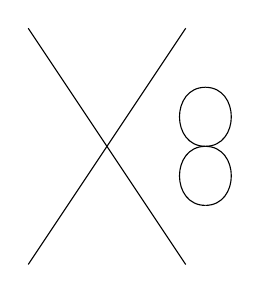
\begin{tikzpicture}
		\begin{feynman}
			% disconnected t-channel diagram
			\vertex (a1) at (0,1.5);
			\vertex (a2) at (0,-1.5);
			\vertex (b1) at (2,1.5);
			\vertex (b2) at (2,-1.5);
			\vertex (c) at (1, 0);

			\diagram*{
				(a1) -- [plain] (c) -- [plain] (b1),
				(a2) -- [plain] (c) -- [plain] (b2),
			};

			\vertex (f1) at (2.25, 0);
			\vertex (fup) at (2.25, 0.75);
			\vertex (fdown) at (2.25, -0.75);

			\diagram*{
				(f1) -- [plain, half left] (fup),
				(f1) -- [plain, half right] (fup),
				(f1) -- [plain, half left] (fdown),
				(f1) -- [plain, half right] (fdown),
			};

		\end{feynman}
	\end{tikzpicture}
	\hspace{3cm}
	
\begin{tikzpicture}
		\begin{feynman}
			% disconnected t-channel diagram
			\vertex (a1) at (0,1.5);
			\vertex (a2) at (0,-1.5);
			\vertex (b1) at (2,1.5);
			\vertex (b2) at (2,-1.5);
			\vertex (c) at (1, 0);

			\diagram*{
				(a1) -- [plain] (c) -- [plain] (b1),
				(a2) -- [plain] (c) -- [plain] (b2),
			};

			\vertex (loopv1) at (1.33, 0.5);  % Place the loop vertex near the upper leg
			\vertex (loopv2) at (1.67, 1);  % Place the loop vertex near the upper leg

			\diagram*{
				(loopv1) -- [plain, half right, min distance=5mm] (loopv2),
			};
		\end{feynman}
	\end{tikzpicture}
	\vspace{5mm}
	\caption{Examples of a disconnected (left) and an un-amputated (right) Feynman diagram.}
	\label{fig:01_qft_interactions_feynman_disconnected}
\end{figure}



\subsubsection{Example: nucleon scattering}

Nucleon-nucleon scattering is the process: $\psi\psi \rightarrow \psi\psi$.
The lowest order at which this can occur is of $\mathcal O(g^2)$, as it requires at least two interaction vertices.
The possible second-order diagrams are shown in Figure~\ref{fig:01_qft_interactions_feynman_nn_scattering}.
We interpret them as nucleons interacting via the exchange of a meson.
As the nucleons are identical, we require two diagrams, for the two permutations of the two final states.

\begin{figure}[ht]
	\centering
	\captionsetup{justification=centering}
	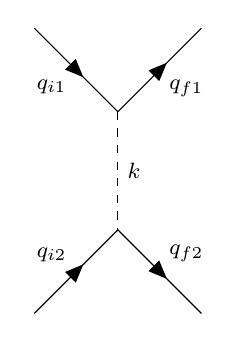
\begin{tikzpicture}
		\begin{feynman}
			\vertex (a);
			\vertex [below=of a] (b);
			\vertex [above left=of a] (i1);
			\vertex [below left=of b] (i2);
			\vertex [above right=of a] (f1);
			\vertex [below right=of b] (f2);
			\diagram* {
				(a) -- [scalar, edge label={\footnotesize$k$}] (b),
				(i1) -- [fermion, edge label'={\footnotesize$q_{i1}$}] (a),
				(i2) -- [fermion, edge label={\footnotesize$q_{i2}$}] (b),
				(a) -- [fermion, edge label'={\footnotesize$q_{f1}$}] (f1),
				(b) -- [fermion, edge label={\footnotesize$q_{f2}$}] (f2),
			};
		\end{feynman}
	\end{tikzpicture}
	\hspace{3cm}
	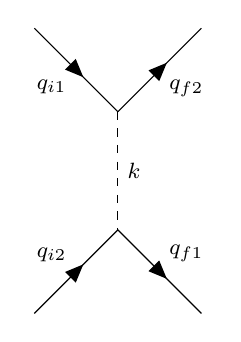
\begin{tikzpicture}
		\begin{feynman}
			\vertex (a);
			\vertex [below=of a] (b);
			\vertex [above left=of a] (i1);
			\vertex [below left=of b] (i2);
			\vertex [above right=of a] (f1);
			\vertex [below right=of b] (f2);
			\diagram* {
				(a) -- [scalar, edge label={\footnotesize$k$}] (b),
				(i1) -- [fermion, edge label'={\footnotesize$q_{i1}$}] (a),
				(i2) -- [fermion, edge label={\footnotesize$q_{i2}$}] (b),
				(a) -- [fermion, edge label'={\footnotesize$q_{f2}$}] (f1),
				(b) -- [fermion, edge label={\footnotesize$q_{f1}$}] (f2),
			};
		\end{feynman}
	\end{tikzpicture}
	\vspace{5mm}
	\caption{The two lowest order nucleon scattering diagrams.}
	\label{fig:01_qft_interactions_feynman_nn_scattering}
\end{figure}

Using the first two Feynman rules, we find
\begin{equation}
	\label{eq:01_qft_interactions_nn_scattering_1}
	i \mathcal M = (-ig)^2 \cdot  \frac{1}{k^2 - m^2 + i\varepsilon}
\end{equation}
for both diagrams.
What remains is to enforce momentum conservation at each vertex.
For the left-most diagram, we see $k = q_{f1} - q_{i1} = q_{f2} - q_{i2}$, while for the right-most $k = q_{f2} - q_{i1} = q_{f1} - q_{i2}$.
Thus, the total matrix element is
\begin{equation}
	\label{eq:01_qft_interactions_nn_scattering_2}
	i \mathcal M = i(\mathcal M_{\mathrm{left}} + \mathcal M_{\mathrm{right}}) = (-ig)^2 \bigg[ \frac{1}{(q_{f1} - q_{i1})^2 - m^2} + \frac{1}{(q_{f2} - q_{i1})^2 - m^2} \bigg],
	% \begin{split}
	% 	i \mathcal M_1 = (-ig)^2 \cdot  \frac{1}{(q_{f1} - q_{i1})^2 - m^2 + i\varepsilon}, \\
	% 	i \mathcal M_2 = (-ig)^2 \cdot  \frac{1}{(q_{f2} - q_{i1})^2 - m^2 + i\varepsilon},
	% \end{split}
\end{equation}
where we have left out the $i\varepsilon$ term as there is no integral to perform.

Generally, we have to be careful with the relative signs of the matrix elements of different diagrams, corresponding to either constructive or destructive interference.
(In fact, Peskin and Schroeder list ``Figure out the overall sign of the diagram'' as a Feynman rule.)
In this case, we can reason physically that since nucleons are bosons, the amplitude will be symmetric under interchange of the two final states, and hence the two diagrams should be summed.

\subsubsection{Mandelstam variables}

To build some intuition for Mandelstam variables, let us sit in the center of mass (COM) frame, and define our coordinate frame such that incoming particles collide along the $z$-axis and scatter in the $y$-$z$ plane:
\begin{equation}
	\label{eq:01_qft_interactions_mandelstam_pcom}
	\begin{split}
		p_{i1} = (E, 0, 0, p) &\qquad p_{i2} = (E, 0, 0, -p) \\
		p_{f1} = (E, 0, p\sin\theta, p\cos\theta) &\qquad p_{f2} = (E, 0, -p\sin\theta, -p\cos\theta).
	\end{split}
\end{equation}
Then,
\begin{equation}
	\label{eq:01_qft_interactions_mandelstam_com}
	s = 4E^2, \quad t = -2p^2(1-\cos\theta), \quad u = -2p^2(1+\cos\theta).
\end{equation}
Thus, $s$ is the total energy in the COM frame squared --- hence, we usually refer to the COM energy as $\sqrt{s}$ --- while $t$ and $u$ are a measure of how much momentum is exchanged between the scattered particles.
For example, if $\theta = 0$, both particles continue in the same direction and $t = 0$, while if $\theta = \pi$, they completely
reverse direction and the momentum transfer along the collision axis is maximized at $\sqrt{\abs{t}} = 2p$.



\section{Spinor field theory}
\label{sec:01_qft_spinors}

\begin{center}
	\centering
	\noindent
	\textit{...anything that comes back to itself with a minus sign after a 2$\pi$ rotation is always going to be a little strange.} --- David Tong~\cite{TongSM}
\end{center}

So far, we have focused on scalar fields, which live in the trivial representation of the Lorentz group and correspond to spin-$0$ bosons.
In this section, we discuss the field theory for spin-$\frac{1}{2}$ particles, or fermions, which constitute all matter in the universe.
% As discussed in Chapter~\ref{sec:01_symmetries_poincare}, all known elementary fermions are associated with \textit{Dirac spinor} fields, which transform under the $(\cnicefrac{1}{2},0) \oplus (0,\cnicefrac{1}{2})$ representation of the Lorentz group.
% We describe the EOM governing free spinor fields, known as the Dirac equation, in Section~\ref{sec:01_qft_spinors_dirac}.
% \TODO{We then...}
% We then quantize the free spinor field in Section~\ref{sec:01_qft_spinors_quantization} and finally discuss Feynman rules for an interacting spinor theory in Section~\ref{sec:01_qft_spinors_feynman}.

\subsection{The Dirac equation}
\label{sec:01_qft_spinors_dirac}

% \subsubsection{Historical development}

Like the Klein-Gordon equation, the Dirac equation was also an attempt at a relativistic version of the Schrödinger equation.
Before the development of QFT, the quantized KG equation was thought to produce negative probabilities due to its second derivative in time.\footnote{We now understand that the KG equation describes perfectly good scalar quantum fields, where the field-theoretic analog of the probability density is in fact the conserved charge of Eq.~\ref{eq:01_qft_quantization_complex_charge}, which is allowed to be negative.}
Dirac thus sought a relativistic \textit{first-order} differential equation in space and time.

Legend has it he was staring into a fire in Cambridge when he came up with an equation of the form
\begin{equation}
	\label{eq:01_qft_spinors_dirac}
	(i\gamma^\mu \partial_\mu - m)\psi = 0,
\end{equation}
where $\gamma^\mu$ are constants that will be defined in a moment, and $\psi$ is a complex field.
It is difficult to make this equation Lorentz covariant; indeed, it is impossible if $\psi$ is a scalar and each $\gamma^\mu$ is simply a number.\footnote{Or even two- or three-dimensional.}
Dirac's brilliant insight, however, was that it \textit{can} be covariant if $\gamma_\mu$ are $4\times 4$ complex matrices and $\psi$ a four component field.

The key is that $\gamma^\mu\partial_\mu$ is essentially the ``square-root'' of the d'Alembertian $\Box$ from the KG-equation:
\begin{equation}
	\label{eq:01_qft_spinors_dirac_wave}
	\gamma^\mu \partial_\mu \gamma^\nu \partial_\nu = \Box = \partial_\mu \partial^\mu,
\end{equation}
if (and only if) $\gamma^\mu$ and $\gamma^\nu$ satisfy the \textit{Clifford algebra}:
\begin{equation}
	\label{eq:01_qft_spinors_clifford_algebra}
	\{\gamma^\mu, \gamma^\nu\} = 2\eta^{\mu\nu},
\end{equation}
where $\{A, B\} = AB + BA$ is the anticommutator.
Dirac found this is possible with $4\times 4$ matrices such as
% Equation~\ref{eq:01_qft_spinors_clifford_algebra} defines \textit{Clifford algebra}, which has irreps only of dimension $4$, such as
\begin{equation}
	\label{eq:01_qft_spinors_gamma_matrices_weyl_basis}
	% \setlength{\arraycolsep}{8pt}
	\gamma^0 = \begin{pmatrix} 0 & \identity \\ \identity & 0 \end{pmatrix}, \quad
	\gamma^i = \begin{pmatrix} 0 & \sigma^i \\ -\sigma^i & 0 \end{pmatrix},
\end{equation}
where $\sigma^i$ are the Pauli matrices (Chapter~\ref{sec:01_symmetries_so3}).
These are called the \textit{gamma}, or \textit{Dirac}, matrices, and plugging them into Eq.~\ref{eq:01_qft_spinors_dirac} yields the \textit{Dirac equation}, which can be written even more compactly by defining $\cslashed{\partial} \equiv \gamma^\mu \partial_\mu$:
\begin{equation}
	\label{eq:01_qft_spinors_dirac_slash}
	(i\cslashed{\partial} - m)\psi = 0.
\end{equation}

This equation is considered one of the most significant breakthroughs in theoretical physics, ``on par with the works of Newton, Maxwell, and Einstein before him''~\cite{hey2003new}.
The insights that followed, as we will outline in this section, provided a theoretical basis for fermion spin, implied the existence of antiparticles, and overall were foundational to the development of the SM.\footnote{These insights were so unexpected that Dirac thought ``his equation was more intelligent than its author''~\cite{brown1983birth}.}

\subsection{Spinors}
\label{sec:01_qft_spinors_spinors}

Before discussing solutions and quantization of the Dirac equation, let us examine what kind of object $\psi$ is.
A related property of the Clifford algebra is that
\begin{equation}
	\label{eq:01_qft_spinors_gamma_lorentz_generators}
	\Sigma_{\mu\nu} \equiv \frac{i}{4}[\gamma^\mu, \gamma^\nu]
\end{equation}
satisfies the Lorentz algebra (Eq.~\ref{eq:01_poincare_algebra_mmunu}).
This means $\Sigma_{\mu\nu}$ are generators of Lorentz transformations
\begin{equation}
	\label{eq:01_qft_spinors_spinor_lorentz_transformation}
	S[\Lambda] = e^{\frac{1}{2}\omega^{\mu\nu}\Sigma_{\mu\nu}},
\end{equation}
where $\Lambda$ is a Lorentz transformation with parameters $\omega^{\mu\nu}$, and $S[\Lambda]$ is a particular 4D representation.

It can be shown\footnote{See e.g. Ref.~\cite{LiuRQFT} Lecture 14.} that the Dirac equation is only Lorentz covariant if the components of $\psi$, $\psi_\alpha$, transform under this exact representation:
\begin{equation}
	\label{eq:01_qft_spinors_spinor_transformation}
	\psi_\alpha \rightarrow \psi'_\alpha = S[\Lambda]^\beta_{\ \alpha} \psi_\beta.
\end{equation}
It is important to note here that $S[\Lambda]$ is acting on the $\psi$ components --- also called the spinor indices -- and not on the spacetime coordinates $x^\mu$, which transform under the vector representation (Eq.~\ref{eq:01_lorentz_generators}).
Explicitly, including the spacetime coordinates, $\psi(x)$ transforms as:
\begin{equation}
	\label{eq:01_qft_spinors_spinor_transformation_x}
	\psi_\alpha(x) \rightarrow \psi'_\alpha(x') = S[\Lambda]^\beta_{\ \alpha} \psi_\beta(\Lambda^{-1}x),
\end{equation}
where both $S[\Lambda]$ and $\Lambda$ share the same transformation parameters $\omega^{\mu\nu}$ and thus correspond to the same Lorentz transformation.\footnote{$x' = \Lambda^{-1}x$ as this is an \textit{active} transformation, in which the field is shifted.}

\subsubsection{Dirac and Weyl spinors}

What is this representation?
Let's look at the rotation and boost generators individually:
\begin{equation}
	\label{eq:01_qft_spinors_spinor_generators}
	\Sigma_{0i} = \frac{i}{2} \begin{pmatrix} -\sigma^i & 0 \\ 0 & \sigma^i \end{pmatrix}, \quad
	\Sigma_{ij} = \frac{1}{2} \epsilon_{ijk} \begin{pmatrix} \sigma^k & 0 \\ 0 & \sigma^k \end{pmatrix}.
\end{equation}
Comparing this with Eqs.~\ref{eq:01_lorentz_irreps_weyl_left} and~\ref{eq:01_lorentz_irreps_weyl_right}, we see that the top left and bottom right blocks are exactly the left- and right-handed Weyl spinor irreps of the generators.
The handedness of a spinor is called its \textit{chirality}, and its physical significance will be discussed in a moment.
Thus, we identify $S[\Lambda]$ with the $(\cnicefrac{1}{2},0) \oplus (0,\cnicefrac{1}{2})$, or Dirac spinor, representation.

This also means that, in this basis of the gamma matrices (called the \textit{Weyl}, or \textit{chiral}, basis), the Dirac spinor $\psi$ can be decomposed into two Weyl spinors:
\begin{equation}
	\label{eq:01_qft_spinors_spinor_decomposition}
	\psi = \begin{pmatrix} \psi_L \\ \psi_R \end{pmatrix},
\end{equation}
which transform under their respective representations.
The two components can be isolated if we consider a fifth gamma matrix:
\begin{equation}
	\label{eq:01_qft_spinors_gamma_five}
	\gamma^5 = i\gamma^0\gamma^1\gamma^2\gamma^3 = \begin{pmatrix} -\identity & 0 \\ 0 & \identity \end{pmatrix}.
\end{equation}
$\gamma^5$ is similar to our main four matrices in that $\{\gamma^5, \gamma^\mu\} = 0$ and $(\gamma^5)^2 = \identity$.
Importantly, we see from its form in the Chiral basis that projection operators $P_L$ and $P_R$ can be defined as:
\begin{equation}
	\label{eq:01_qft_spinors_chiral_projection}
	P_L = \frac{1 - \gamma^5}{2}, \quad P_R = \frac{1 + \gamma^5}{2},
\end{equation}
which satisfy the projection property $P_{L/R}^2 = P_{L/R}$ and project out the left- and right-handed components of a Dirac spinor:
\begin{equation}
	\label{eq:01_qft_spinors_chiral_projection_action}
	P_{L} \begin{pmatrix} \psi_L \\ \psi_R \end{pmatrix} = \begin{pmatrix} \psi_L \\ 0 \end{pmatrix}, \quad P_{R} \begin{pmatrix} \psi_L \\ \psi_R \end{pmatrix} = \begin{pmatrix} 0 \\ \psi_R \end{pmatrix}.
\end{equation}
Note that while the specific form depends on the basis, the definitions in Eq.~\ref{eq:01_qft_spinors_chiral_projection} are basis-independent and can be considered to define chirality.

\subsubsection{Chirality}

The two Weyl spinor representations are related by a complex conjugation, meaning $\psi_L^*$ is a right-handed Weyl spinor, and vice versa.
For a complex scalar field, we interpreted the conjugate as the antiparticle.
The same interpretation applies here; hence, if a left-handed spinor describes a particle, its antiparticle is described by its conjugate, right-handed spinor.

The Dirac equation can be rewritten in the Weyl basis as two coupled equations of the Weyl spinors.
Let us define $\sigma^\mu = (\identity, \cvec{\sigma})$ and $\bar{\sigma}^\mu = (\identity, -\cvec{\sigma})$, so that
\begin{equation}
	\label{eq:01_qft_spinors_dirac_weyl}
	(i\gamma^\mu\partial_\mu - m)\psi =
	\begin{pmatrix}
		-m & i\sigma^\mu\partial_\mu \\ i\bar{\sigma}^\mu\partial_\mu & -m
	\end{pmatrix}
	\begin{pmatrix} \psi_L \\ \psi_R \end{pmatrix} = 0.
\end{equation}
Hence, we see the mass term couples the left- and right-handed components.
This is why all massive fermions must exist in pairs of particles and antiparticles.
An important special case, however, is for a neutral \textit{Majorana} fermion, where $\psi$ equals its charge conjugate $\psi^c$ (to be defined below).
Such a particle is its own antiparticle and can have a left-handed- or right-handed-only mass term.
As discussed in Chapter~\ref{sec:01_symmetries_poincare}, the only Majorana candidate in the SM is the right-handed neutrino.

For $m = 0$, the Dirac equation decouples and leaves us with the \textit{Weyl equations} describing massless fermions:
\begin{equation}
	\label{eq:01_qft_spinors_weyl}
	i\sigma^\mu\partial_\mu \psi_R= 0, \quad i\bar{\sigma}^\mu\partial_\mu \psi_L = 0.
\end{equation}
In Fourier space, these are:
\begin{equation}
	\label{eq:01_qft_spinors_weyl_fourier}
	\begin{split}
		\sigma^\mu p_\mu \psi_R = (E - \cvec{\sigma}\cdot\cvec{p})\psi_R = 0 \quad \Rightarrow \quad  \frac{\cvec{\sigma}\cdot\cvec{p}}{\abs{\cvec{p}}}\, \psi_R = +\psi_R, \\
		\bar{\sigma}^\mu p_\mu \psi_L = (E + \cvec{\sigma}\cdot\cvec{p})\psi_L = 0 \quad \Rightarrow \quad \frac{\cvec{\sigma}\cdot\cvec{p}}{\abs{\cvec{p}}}\, \psi_L = -\psi_L,
	\end{split}
\end{equation}
where we used $E = \abs{\cvec{p}}$ for massless particles.
You may recall $\frac{\cvec{\sigma}\cdot\cvec{p}}{\abs{\cvec{p}}}$ is the helicity operator, projecting the particle spin along its momentum.
Thus, in the massless limit, we see that the left- and right-handed Weyl spinors are the $+1$ and $-1$ helicity eigenstates, respectively.

This is not the case for massive particles, as helicity is no longer Lorentz invariant: one can always boost into a frame where the momentum is inverted while the spin remains the same, changing the sign of the helicity.
Chirality is thus a more abstract concept for massive particles, related only to how they transform under Lorentz transformations.

Theories not symmetric under exchange of left- and right-handed components are called \textit{chiral}, and symmetric theories \textit{vector}.
QED and QCD are both vector theories, but weak interactions are, surprisingly, chiral.
This necessarily means it violates parity and charge conjugation symmetries ($P$ and $C$), which we will discuss soon in Section~\ref{sec:01_qft_spinors_cpt}.


\subsection{The Dirac Lagrangian}
\label{sec:01_qft_spinors_lagrangian}

Recall that to quantize the scalar theory, we first needed the Lagrangian and the classical solutions of the K-G equation, to then obtain Hamiltonian and canonical fields and Poisson brackets before finally promoting them to quantum commutatation relations.
We will proceed in similar (though condensed) fashion for the spinor theory, and first derive the Lagrangian corresponding to the Dirac equation.

Since we are no longer dealing with trivial representation of the Lorentz group, we have to be more careful with the types of terms we put into the Lagrangian; it must be composed of good Lorentz-invariant objects.
% The action is Lorentz invariant, so the Lagrangian must be composed of good Lorentz-covariant objects.
A first guess at a Lorentz scalar formed of spinors may be $\psi^\dagger\psi$.
This is indeed a scalar, but it is \textit{not} Lorentz invariant:
$\psi$ and $\psi^\dagger$ transform as $\psi\rightarrow S[\Lambda]\psi$, $\psi^\dagger\rightarrow \psi^\dagger S[\Lambda]^\dagger$ and, hence
\begin{equation}
	\label{eq:01_qft_spinors_lagrangian_scalar_wrong}
	\psi^\dagger\psi \rightarrow \psi^\dagger S[\Lambda]^\dagger S[\Lambda]\psi. % \neq \psi^\dagger\psi.
\end{equation}
However, recall from Chapter~\ref{sec:01_symmetries_poincare} that (finite-dimensional) representations of Lorentz transformations are not unitary.
(We can see this as well from the fact that the generators of $S[\Lambda]$ in Eq.~\ref{eq:01_qft_spinors_spinor_generators} are not anti-Hermitian.)
Thus, $S[\Lambda]^\dagger S[\Lambda] \neq 1$ in general and $\psi^\dagger\psi$ is not a Lorentz scalar.

Instead, with a bit of matrix algebra\footnote{See e.g. Schwartz~\cite{Schwartz:2014sze} Chapter 10.3}, one can show that
\begin{equation}
	\label{eq:01_qft_spinors_gamma0_inverse}
	\gamma^0 S[\Lambda] \gamma^0 = (S[\Lambda]^{-1})^\dagger,
\end{equation}
and hence
\begin{equation}
	\label{eq:01_qft_spinors_lagrangian_scalar}
	\psi^\dagger\gamma^0\psi \rightarrow \psi^\dagger S[\Lambda]^\dagger \gamma^0 S[\Lambda]\psi = \psi^\dagger\gamma^0 S[\Lambda]^{-1} S[\Lambda]\psi = \psi^\dagger\gamma^0\psi
\end{equation}
\textit{is} a Lorentz scalar.
Thus, we define $\bar\psi \equiv \psi^\dagger\gamma^0$ as the ``natural'' conjugate to $\psi$, and end up with a nice Lorentz scalar $\bar\psi \psi$ for our Lagrangian.

Similarly, one can show that $\bar\psi\gamma^\mu\psi$ transforms as a Lorentz $4$-vector and, hence, contracting it with $\partial_\mu$ as $\bar\psi\gamma^\mu\partial_\mu\psi$ yields another scalar.
These two terms, which are analogous to the mass and derivative terms a free complex scalar field (Eq.~\ref{eq:01_qft_symmetries_complex_lagrangian}), are enough to build the Dirac Lagrangian:
\begin{equation}
	\label{eq:01_qft_spinors_lagrangian}
	\mathcal{L} = i\bar\psi\gamma^\mu\partial_\mu\psi - m\bar\psi\psi = \bar\psi(i\cslashed{\partial} - m)\psi.
\end{equation}
One can check that the EL equations reproduce the Dirac equation for $\psi$ and $\bar\psi$.

\subsubsection{The U(1) conserved current}

As with the complex scalar field, observe that the Dirac Lagrangian is invariant under global \UU[1] symmetry $\psi \rightarrow e^{i\alpha}\psi$.
Using Noether's theorem, we can derive the conserved current and charge associated with this symmetry:
\begin{equation}
	\label{eq:01_qft_spinors_lagrangian_current}
	j^\mu = \bar\psi\gamma^\mu\psi, \quad Q = \int d^3x\, j^0 = \int d^3x\, \psi^\dagger\psi.
\end{equation}
As for the complex scalar field, these represent the electromagnetic $4$-current and charge, respectively --- a connection we will explore further in Section~\ref{sec:01_qft_gt_maxwell}.


\subsection{Quantizing the Dirac field}
\label{sec:01_qft_spinors_quantization}

\subsubsection{Solutions to the Dirac equation}

Before quantizing, we first need the classical solutions to the Dirac equation.
Multiplying both sides of it by $-(i\gamma^\mu\partial_\mu + m)$ gives us:
\begin{equation}
	\label{eq:01_qft_spinors_dirac_squared}
	-(i\gamma^\mu\partial_\mu + m)(i\gamma^\nu\partial_\nu - m)\psi = (\Box - m^2)\psi = 0,
\end{equation}
which means each component of $\psi$ individually satisfies the KG-equation.
Thus, we can assume similar plane wave solutions:
\begin{equation}
	\label{eq:01_qft_spinors_dirac_solution}
	\psi(x) = \int \frac{d^3p}{(2\pi)^3} \, u(p) e^{-ip\cdot x} + v(p) e^{ip\cdot x},
\end{equation}
where $u(p)$ and $v(p)$ are now spinors, and again we have positive and negative frequency solutions that correspond to particles and antiparticles, respectively, after quantization.

One can check using Fourier space, as we did for the Weyl equations, that
\begin{equation}
	\label{eq:01_qft_spinors_dirac_solution_up}
	u(p) = \begin{pmatrix} \sqrt{p \cdot \sigma}\, \xi \\ \sqrt{p \cdot \bar\sigma}\, \xi \end{pmatrix}, \quad
	v(p) = \begin{pmatrix} \sqrt{p \cdot \sigma}\, \eta \\ -\sqrt{p \cdot \bar\sigma}\, \eta \end{pmatrix}
\end{equation}
are general solutions to the Dirac equation, where $\xi$ and $\eta$ are the familiar two-component spinors from QM for spin-$\cnicefrac{1}{2}$ particles (although technically they do not have this interpretation before quantization).
As is conventional, we will use a basis of $\sigma_z$ eigenstates $\xi_1 = \eta_1 = (1, 0)^T$ and $\xi_2 = \eta_2 = (0, 1)^T$, corresponding to spin-up and spin-down, respectively.
% , with eigenvalues $+1$ and $-1$, respectively.

For example, in the rest frame $p_\mu = (m, 0, 0, 0)$, we have:
\begin{equation}
	\label{eq:01_qft_spinors_dirac_solution_rest}
	u(p)_1 = \sqrt{m} \begin{pmatrix} 1 \\ 0 \\ 1 \\ 0 \end{pmatrix}, \,
	u(p)_2 = \sqrt{m} \begin{pmatrix} 0 \\ 1 \\ 0 \\ 1 \end{pmatrix}, \,
	v(p)_1 = \sqrt{m} \begin{pmatrix} 1 \\ 0 \\ -1 \\ 0 \end{pmatrix}, \,
	v(p)_2 = \sqrt{m} \begin{pmatrix} 0 \\ 1 \\ 0 \\ -1 \end{pmatrix}.
\end{equation}
More generally, we can always orient a particle's 3-momentum along the $z$-axis, in which case:
\begin{equation}
	\label{eq:01_qft_spinors_dirac_solution_momentum}
\resizebox{\textwidth}{!}{$
	u(p)_1 = \begin{pmatrix} \sqrt{E - p_z} \\ 0 \\ \sqrt{E + p_z} \\ 0 \end{pmatrix}, \quad
	u(p)_2 = \begin{pmatrix} 0 \\ \sqrt{E - p_z} \\ 0 \\ \sqrt{E + p_z} \end{pmatrix} \quad
	v(p)_1 = \begin{pmatrix} \sqrt{E + p_z} \\ 0 \\ -\sqrt{E - p_z} \\ 0 \end{pmatrix}, \quad
	v(p)_2 = \begin{pmatrix} 0 \\ \sqrt{E + p_z} \\ 0 \\ -\sqrt{E - p_z} \end{pmatrix}.
$}
\end{equation}

\subsubsection{Quantization}

Now that we have a sensible Lagrangian and the classical solutions to the Dirac equation, the remaining steps to quantization follow closely that for our complex scalar field in Section~\ref{sec:01_qft_quantization_complex}, but with two notable differences.
The first is that we now must sum over the two spin components of $u_s(p)$ and $v_s(p)$, in addition to integrating over the momentum:
\begin{equation}
	\label{eq:01_qft_spinors_quantization}
	\begin{split}
		\psi(x) &= \sum_{s = 1, 2} \int \frac{d^3p}{(2\pi)^3} \left[\hat b^s_{\cvec{p}}\, u_s(p) e^{-ip\cdot x} + c^{s\dagger}_{\cvec{p}}\, v_s(p) e^{ip\cdot x}\right], \\
		\bar\psi(x) &= \sum_{s = 1, 2} \int \frac{d^3p}{(2\pi)^3} \left[\hat b^{s\dagger}_{\cvec{p}}\, \bar{u}_s(p) e^{ip\cdot x} + \hat c^s_{\cvec{p}}\,  \bar{v}_s(p) e^{-ip\cdot x}\right].
	\end{split}
\end{equation}
As before, we have positive and negative frequency solutions, with the $b/b^\dagger$ and $c/c^\dagger$ operators associated with particles of the same mass and opposite charge.

For spinors, we find that the $\hat b^{s\dagger} \ket{0}$ and $\hat c^{s\dagger} \ket{0}$ also have opposite spins, i.e. for the $z$-axis angular momentum operator $J_z$ (which can be derived through Noether's theorem as we did for the momentum operator in Section~\ref{sec:01_qft_classical_symmetries}):
\begin{equation}
	\label{eq:01_qft_spinors_spin_z}
	J_z\, \hat b^{s\dagger} \ket{0} = \pm\frac{1}{2} \hat b^{s\dagger} \ket{0}, \quad J_z\, \hat c^{s\dagger}\ket{0} = \mp \frac{1}{2} \hat c^{s\dagger}\ket{0}.
\end{equation}
By convention, we take $b^{s\dagger}$ and $b^s$ to be the creation and annihilation operators for the electron, and $c^{s\dagger}$ and $c^s$ for its antiparticle, the positron.
Thus, $\bar\psi_s(x)\ket{0}$ corresponds to an electron at $x$ with spin state $s$, and $\psi_s(x)\ket{0}$ to a positron at $x$ with the opposite spin state to $s$.

Through his equation, Dirac was the first to predict the existence of antimatter in 1930~\cite{Dirac:1930ek} (although he initially thought the electron's antiparticle was the proton).
This prediction was soon confirmed by the discovery of a particle with the same mass as the electron but opposite charge by Carl Anderson in a bubble chamber in 1932~\cite{Anderson:1932zz}.
Both were awarded the Nobel prize.

% made shocking prediction, and they were discovered.
% particles created by b have same mass as by a, but opposite charge and spin (?).

\subsubsection{The spin-statistics connection}

The second, extremely important difference from scalar quantization is that, because spinors are spin-$\frac{1}{2}$ particles, they must obey \textit{anticommutation relations}:
\begin{equation}
	\label{eq:01_qft_spinors_anticommutation}
	\begin{split}
		\{\psi_\alpha(x), \psi_\beta(y)\} =& \,\{\bar\psi_\alpha(x), \bar\psi_\beta(y)\} = 0, \\
		\{\psi_\alpha(x), \bar\psi_\beta(y)\} &= \delta_{\alpha\beta}\delta^3(\cvec{x} - \cvec{y}),
	\end{split}
\end{equation}
which also means the creation and annihilation operators satisfy:
\begin{equation}
	\label{eq:01_qft_spinors_anticommutation_operators}
	% \{a_s(p), a_{r}^\dagger(q)\} = \{b_s(p), b_{r}^\dagger(q)\} = (2\pi)^3\delta^3(\cvec{p} - \cvec{q})\delta_{sr}.
	\{\hat b^{s}_{\cvec{p}}, \hat b^{r\dagger}_{\cvec{q}}\} = \{\hat c^{s}_{\cvec{p}}, \hat c^{r\dagger}_{\cvec{q}}\} = (2\pi)^3\delta^3(\cvec{p} - \cvec{q})\delta_{sr}.
\end{equation}
Thus, unlike bosons, exchanging two particles yields a minus sign: $\hat b^{r\dagger}_{\cvec{p}_1} \hat b^{s\dagger}_{\cvec{p}_1} \ket{0} = -\hat b^{s\dagger}_{\cvec{p}_2} \hat b^{r\dagger}_{\cvec{p}_1} \ket{0}$, confirming that spinors obey Fermi-Dirac statistics and obey the Paul-Exclusion principle.

Were we to try and impose our earlier commutation relations for spinors (or indeed, any half-integer-spin field), we would run into several issues.
These include the time-ordered product in the $S$-matrix not being Lorentz invariant, and antiparticles contributing arbitrarily negative energies, making the theory unstable.
They are all related to the deep connection between spin and statistics: the requirement of Lorentz invariance, stability, and causality in a QFT necessitates that half-integer-spin particles obey Fermi-Dirac, and integer-spin particles Bose-Einstein statistics.\footnote{For more detailed discussion, see e.g. Peskin and Schroeder~\cite{Peskin:1995ev} Chapter 3.5 and Schwartz~\cite{Schwartz:2014sze} Chapter 12.}


\subsection{Interactions and Feynman rules}
\label{sec:01_qft_spinors_feynman}

Having quantized the free Dirac field, we now discuss interactions, again focusing on small (and renormalizable) perturbations to the free theory.
% \TODO{fix this...} As one may expect, the primary difference with respect to the complex scalar ``nucleon'' fields from Section~\ref{sec:01_qft_quantization_interactions} is
We start by presenting the propagators for the Dirac field and then extending our scalar Yukawa theory from Section~\ref{sec:01_qft_interactions} to spinor ``nucleons''.

\subsubsection{Propagators}

We define the propagator for the Dirac field the same as for scalar fields in Section~\ref{sec:01_qft_quantization_propagators}:
% Recall from Section~\ref{sec:01_qft_quantization_propagators} that the propagator between spacetime points $x$ and $y$ is:
\begin{equation}
	\label{eq:01_qft_spinors_propagator}
	D_{\alpha\beta}(x - y) = \bra{0}\psi(x)_\alpha\bar\psi(y)_\beta\ket{0} = \int \frac{d^3p}{(2\pi)^3} \frac{1}{2E_p} \sum_s u^s_\alpha(p) \bar u^s_\beta(p) e^{-ip\cdot(x - y)},
\end{equation}
where $\alpha$ and $\beta$ index the spinor components.
Again, we have an extra sum over the spin states.
With some more matrix algebra one can show that these kinds of sums simplify nicely to
\begin{equation}
	\label{eq:01_qft_spinors_uvsum}
	\sum_s u^s_\alpha(p) \bar u^s_\beta(p) = (\cslashed{p} + m)_{\alpha\beta}, \quad \sum_s v^s_\alpha(p) \bar v^s_\beta(p) = (\cslashed{p} - m)_{\alpha\beta},
\end{equation}
so that we end up with, in momentum space, the Feynman propagator:
\begin{equation}
	\label{eq:01_qft_spinors_propagator_momentum}
	\Delta_F(p) \equiv \bra{0}T\psi(x)\bar\psi(y)\ket{0} =  \frac{i(\cslashed{p} + m)}{p^2 - m^2 + i\epsilon}.
\end{equation}
Note that we have now suppressed the spinor indices; $\Delta_F$ is still a $4\times4$ matrix in spinor space.
Note as well the relative minus sign in the time-ordering operator for fermions, due to exchanging the fields:
\begin{equation}
	\label{eq:01_qft_spinors_propagator_time_ordering}
	\bra{0}T\psi(x)\bar\psi(y)\ket{0} = \begin{cases} \bra{0}\psi(x)\bar\psi(y)\ket{0} & x^0 > y^0, \\ -\bra{0}\bar\psi(y)\psi(x)\ket{0} & x^0 < y^0. \end{cases}
\end{equation}

\subsubsection{External lines}

For scalars, external line terms such as $\phi \ket{p}$ simply contributed a factor of $1$ to the matrix element, where $\ket{p}$ is again a one-particle meson state with momentum $p$:
\begin{equation}
	\label{eq:01_qft_spinors_yukawa_scalar_external}
	\phi \ket{p} \sim \int \frac{d^3p'}{(2\pi)^3} \frac{1}{\sqrt{2E_{p'}}} a_{\cvec{p}'} e^{-ip'\cdot x} \sqrt{2E_{p}}\, a_{\cvec{p}}^\dagger \ket{0} = e^{-ip\cdot x} \ket{0}.
\end{equation}
(The $e^{-ip\cdot x}$ factor contributes only to the momentum conservation delta function in the $S$-matrix element.)
For spinors, we instead end up with a spinor factor.
For example, for an incoming fermion with momentum $q$ and spin $s$:
\begin{equation}
	\label{eq:01_qft_spinors_yukawa_spinor_external}
	\psi \ket{q, s} \sim \int \frac{d^3q'}{(2\pi)^3} \frac{1}{\sqrt{2E_{q'}}} \sum_s' b^{s'}_{\cvec{q}'} u^{s'}(q') e^{-iq'\cdot x} \sqrt{2E_{q}}\, b^{s\dagger}_{\cvec{q}} \ket{0} = u^s(q) e^{-iq\cdot x} \ket{0}.
\end{equation}
We can see looking at the form of the quantized fields (Eq.~\ref{eq:01_qft_spinors_quantization}), and which terms will contribute something non-zero, that incoming (outgoing) external fermions will be associated with a $u$ $(\bar u$) and antifermions with a $\bar v$ $(v$) factor.\footnote{The ``$\sim$'' becomes an ``$=$'' for a \textit{Wick contraction}, $\contraction{}{\phi}{}{\ket{p}} \phi \ket{p}$, which is what we deal with with time-ordered operator products.}

\subsubsection{Yukawa theory reloaded}

We now revisit Yukawa theory, the simplest possible theory of interactions for spinors.
The Lagrangian is the same as in Eq.~\ref{eq:01_qft_interactions_yukawa}, but now with $\psi$ a spinor:
\begin{equation}
	\label{eq:01_qft_spinors_yukawa_lagrangian}
	\mathcal{L} = \frac{1}{2}\partial^\mu\phi\partial_\mu\phi + i\bar\psi\cslashed{\partial}\psi - \frac{1}{2}m^2\phi^2 - M\bar\psi\psi - g\phi\bar\psi\psi.
\end{equation}
Note that through dimensional analysis, since $[M\bar\psi\psi] = [\bar\psi\cslashed{\partial}\psi] \mustequal 4$ we can deduce that $[\psi] = \frac{3}{2}$.
This means that (1) the Yukawa interaction is marginal, with $[\phi\bar\psi\psi] = 4$ and $[g] = 0$, and (2) importantly, there are no other renormalizable, Lorentz-invariant interactions we can write down for spinors with the fields at our disposal (modulo some $\gamma^5$'s thrown in, as we'll discuss in Section~\ref{sec:01_qft_spinors_cpt}).
Terms like $\psi\phi^2$, $\cslashed{\partial}\psi\phi$, or $\bar\psi\psi\phi^2$ are all either not Lorentz-scalars or of dimension $\geq 5$.
In this sense, because their possible interactions are so heavily constrained by their $\frac{3}{2}$-dimensionality, spinors in QFT are quite simple!
There is only one other spinor interaction in the SM, which we will see in Section~\ref{sec:01_qft_gt}, with gauge bosons.

We again refer to $\phi$ and $\psi$ as the ``meson'' and ``nucleon'' fields, which is slightly more accurate now since nucleons are in reality fermions.
The two main features missing from this theory are that the relevant mesons, the pions, are \textit{pseudoscalars} (to be discussed in the next section) and are a strong isospin triplet (to be described briefly in Chapter.~\ref{sec:01_sm_qcd}).
% However, \TODO{pseudo-scalar, isospin?}.

\begin{definition}
	\label{def:01_qft_spinors_yukawa_feynman}
	The Feynman rules in momentum space for spinor Yukawa theory are:
	\begin{enumerate}
	\item Vertices: \qquad
	\begin{tikzpicture}[baseline={([yshift=-0.8ex]current bounding box.center)}]
		\begin{feynman}[small]
			\vertex (a);
			\vertex [right=of a] (b);
			\vertex [above right=of b] (f1);
			\vertex [below right=of b] (f2);
			\diagram* {
				(a) -- [scalar] (b),
				(b) -- [fermion] (f1),
				(b) -- [anti fermion] (f2),
			};
		\end{feynman}
	\end{tikzpicture}
	$ = -ig$ \\[1em]
	\item Internal lines (propagators) \\[1em]
	\qquad\qquad Mesons: \quad
	\begin{tikzpicture}[baseline={([yshift=-1.8ex]current bounding box.center)}]
		\begin{feynman}[small]
			\vertex (a);
			\vertex [right=of a] (b);
			\diagram* {
				(a) -- [scalar, edge label={\footnotesize$p$}] (b) ,
			};
		\end{feynman}
	\end{tikzpicture}
	$\, = \cfrac{i}{p^2 - m^2 + i\varepsilon}$ \qquad
	Nucleons: \quad
	\begin{tikzpicture}[baseline={([yshift=-1.8ex]current bounding box.center)}]
		\begin{feynman}[small]
			\vertex (a);
			\vertex [right=of a] (b);
			\diagram* {
				(a) -- [fermion, edge label={\footnotesize$q$}] (b),
			};
		\end{feynman}
	\end{tikzpicture}
	$\, = \cfrac{i(\cslashed{q} + m)}{q^2 - M^2 + i\varepsilon}$ \\[1em]
	\item External lines (on-shell particles)  \\
    % \\[1.5em]
    % % \hspace*{-\leftmargini}
    % \begin{minipage}{0.99\textwidth}
    \begin{tabbing}
    Incoming mesons: 
    \hspace*{1.5cm}
    \=
	\begin{tikzpicture}[baseline={([yshift=-0.8ex]current bounding box.center)}]
		\begin{feynman}[small]
			\vertex (a);
			\vertex [right=of a] (b);
			\vertex [above right=of b] (f1);
			\vertex [below right=of b] (f2);
			\diagram* {
				(a) -- [scalar] (b),
				(b) -- [fermion] (f1),
				(b) -- [anti fermion] (f2),
			};
		\end{feynman}
	\end{tikzpicture}
    \hspace*{0.5cm}
    \=
    $ = 1$
    \\[1.5em]
    Outgoing mesons: 
    % \hspace*{1.5cm}
    \>
    \begin{tikzpicture}[baseline={([yshift=-0.8ex]current bounding box.center)}]
        \begin{feynman}[small]
            \vertex (a);
            \vertex [right=of a] (b);
            \vertex [above left=of a] (f1);
            \vertex [below left=of a] (f2);
            \diagram* {
                (f1) -- [fermion] (a),
                (f2) -- [anti fermion] (a),
                (a) -- [scalar] (b),
            };
        \end{feynman}
    \end{tikzpicture}
    % \hspace*{0.2cm}
    \>
    $ = 1$ \\[1.5em]
    Incoming nucleons: 
    % \hspace*{1.5cm}
    \>
    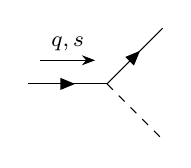
\begin{tikzpicture}[baseline={([yshift=-0.8ex]current bounding box.center)}]
        \begin{feynman}[small]
            \vertex (a);
            \vertex [right=of a] (b);
            \vertex [above right=of b] (f1);
            \vertex [below right=of b] (f2);
            \diagram* {
                (a) -- [fermion, momentum={\footnotesize$q, s$}] (b),
                (b) -- [fermion] (f1),
                (b) -- [scalar] (f2),
            };
        \end{feynman}
    \end{tikzpicture}
    % \hspace*{0.2cm}
    \>
    $ = u_s(q)$
    \\[1.5em]
    Outgoing nucleons: 
    \>
    % \hspace*{1.5cm}
    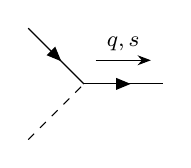
\begin{tikzpicture}[baseline={([yshift=-0.8ex]current bounding box.center)}]
        \begin{feynman}[small]
            \vertex (a);
            \vertex [right=of a] (b);
            \vertex [above left=of a] (f1);
            \vertex [below left=of a] (f2);
            \diagram* {
                (f1) -- [fermion] (a),
                (f2) -- [scalar] (a),
                (a) -- [fermion, momentum={\footnotesize$q, s$}] (b),
            };
        \end{feynman}
    \end{tikzpicture}
    \>
    $ = \bar{u}_s(q)$
    \\[1.5em]
    Incoming antinucleons: 
    \>
    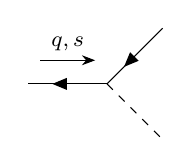
\begin{tikzpicture}[baseline={([yshift=-0.8ex]current bounding box.center)}]
        \begin{feynman}[small]
            \vertex (a);
            \vertex [right=of a] (b);
            \vertex [above right=of b] (f1);
            \vertex [below right=of b] (f2);
            \diagram* {
                (a) -- [anti fermion, momentum={\footnotesize$q, s$}] (b),
                (b) -- [anti fermion] (f1),
                (b) -- [scalar] (f2),
            };
        \end{feynman}
    \end{tikzpicture}
    \>
    $ = \bar{v}_s(q)$
    \\[1.5em]
    Outgoing antinucleons: 
    \>
    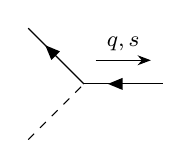
\begin{tikzpicture}[baseline={([yshift=-0.8ex]current bounding box.center)}]
        \begin{feynman}[small]
            \vertex (a);
            \vertex [right=of a] (b);
            \vertex [above left=of a] (f1);
            \vertex [below left=of a] (f2);
            \diagram* {
                (f1) -- [anti fermion] (a),
                (f2) -- [scalar] (a),
                (a) -- [anti fermion, momentum={\footnotesize$q, s$}] (b),
            };
        \end{feynman}
    \end{tikzpicture}
    \>
    $ = v_s(q)$
    \end{tabbing}
	\item Impose momentum conservation at each vertex.
	\item Integrate over the momentum $k$ flowing through each loop.
	\item Figure out the sign based on statistics.
\end{enumerate}
\end{definition}

\subsubsection{Meson decay and the Higgs decay width}

\begin{figure}[ht]
	\centering
    % \captionsetup{justification=centering}
	\begin{tikzpicture}
		\begin{feynman}
			\vertex (a) {$\phi$};
			\vertex [right=of a] (b);
			\vertex [above right=of b] (f1) {$\bar u_{s_1}(q_1)$};
			\vertex [below right=of b] (f2) {$v_{s_2}(q_2)$};
			\diagram* {
				(a) -- [scalar] (b),
				(b) -- [fermion] (f1),
				(b) -- [anti fermion] (f2),
			};
		\end{feynman}
	\end{tikzpicture}
    \vspace{3mm}
    \caption{Tree-level Feynman diagram for meson decay via a Yukawa interaction.}
	\label{fig:01_qft_spinors_meson_decay}
\end{figure}


The matrix element for meson decay into a fermion-antifermion pair with spin and momentum $s_1, q_1$ and $s_2, q_2$, respectively, to first-order can be read off from the Feynman diagram in Figure~\ref{fig:01_qft_spinors_meson_decay}:
\begin{equation}
	\label{eq:01_qft_spinors_meson_decay_m}
	i \mathcal M = -ig\bar u_{s_1}(q_1) v_{s_2}(q_2)
\end{equation}

We can calculate the decay rate as in Section~\ref{sec:01_qft_interactions_decay}, except now we have to sum over the spins of the fermions:
\begin{equation}
	\label{eq:01_qft_spinors_meson_decay_rate}
	d\Gamma = \sum_{s_1, s_2}^2 \frac{1}{2m} \abs{\mathcal M}^2 d\Pi_{\mathrm{LIPS}} = \frac{g^2}{2m} \sum_{s_1, s_2}^2 \abs{\bar u_{s_1}(q_1) v_{s_2}(q_2)}^2 d\Pi_{\mathrm{LIPS}}.
\end{equation}
In the COM frame, we can choose $q_1 = (\frac{m}{2}, 0, 0, q)$ and $q_2 = (\frac{m}{2}, 0, 0, -q)$, with $q^2 = \frac{m^2}{4} - M^2$ by energy conservation.
Using the forms of $\bar u_s$ and $v_s$ we found in Eq.~\ref{eq:01_qft_spinors_dirac_solution_momentum}, we see that the sum over spin states simplifies nicely:
\begin{equation}
	\label{eq:01_qft_spinors_meson_decay_sum}
	\sum_{s_1, s_2}^2 \abs{\bar u_{s_1}(q_1) v_{s_2}(q_2)}^2 = 8q^2 = 2(m^2 - 4M^2).
\end{equation}
Since this is independent of the final state kinematics, the integral of $d\Pi_{\mathrm{LIPS}}$ is the same as for the scalar meson decay, and we obtain an the overall decay rate of:
\begin{equation}
	\label{eq:01_qft_spinors_meson_decay_rate_final}
	\Gamma = \frac{g^2m}{16\pi} \left(1 - \frac{4M^2}{m^2}\right)^{3/2}.
\end{equation}

As we hinted at in Section~\ref{sec:01_qft_interactions_decay}, this is in fact the decay width of the Higgs boson to fermions at tree level, if we plug in the Higgs Yukawa coupling constant $g_f = \cnicefrac{\sqrt{2} m_f}{v}$.
Here $m_f$ is the fermion mass and $v$ is the Higgs vacuum expectation value, $246\GeV$.
For example, for the $H\to \mu^+\mu^-$ decay, with $M = m_\mu = 105.7\MeV$ and $m = m_H = 125\GeV$, we get $\Gamma \approx 900\eV$, exactly in line with the predicted value~\cite{Denner:2011mq}!

One can similarly update our nucleon scattering amplitudes from Section~\ref{sec:01_qft_interactions_feynman}, which simply gain some inner products between the incoming and outgoing spin states (see e.g. Tong QFT~\cite{TongQFT} Chapter 5.7).
Notably, however, the $t$-channel and $u$-channel diagrams (Figure~\ref{fig:01_qft_interactions_feynman_nn_scattering}) now have a relative \textit{minus} sign, in accordance with Fermi-Dirac statistics.


\subsection{CPT Symmetries}
\label{sec:01_qft_spinors_cpt}

In this section, we discuss three important \textit{discrete} symmetries in QFT.
As discussed in Chapter~\ref{sec:01_symmetries_poincare}, the full Lorentz group includes the parity $P$ and time reversal $T$ operators.
In the $4$-vector representation, they have the simple forms $P = \diag(1, -1, -1, -1)$ and $T = \diag(-1, 1, 1, 1)$, meaning
\begin{equation}
	\label{eq:01_qft_spinors_pt4v}
	P: (t, \cvec{x}) \rightarrow (t, -\cvec{x}), \quad T: (t, \cvec{x}) \rightarrow (-t, \cvec{x}).
\end{equation}
However, their forms in other representations, such as spinors, are not as straightforward.

Observe also that all our complex Lagrangians so far have been invariant under some form of complex conjugation $\psi \leftrightarrow \psi^*$.
This represents another discrete symmetry, and since we know from Eq.~\ref{eq:01_qft_symmetries_u1_transformation} that complex conjugation inverts ``charge'', we call this charge conjugation, or $C$, symmetry.

All local, relativistic QFTs are necessarily invariant under the combined $CPT$ symmetry; this is known as the CPT theorem~\cite{Schwinger:1951xk, Luders:1954zz}.\footnote{One way to convince yourself of this is to check that all possible Lorentz scalar terms in the Lagrangian are invariant under $CPT$, as shown in Peskin and Shroeder~\cite{Peskin:1995ev} Chapter 3.6.}
Whether a theory is individually $C$, $P$, or $T$ invariant, however, must be determined by experiment,\footnote{And also somewhat by the requirement of anomaly cancellation; see e.g. Tong SM~\cite{TongSM} Chapter 4.} as we give examples of below.
If it is, we must impose the symmetries in our mathematical formulation by carefully defining the actions of the relevant operators; i.e., we have to consider how $\psi$ must transform under $P$ to maintain $P$-invariance of the Lagrangian, etc.

Such symmetries are crucial handles for understanding QFTs, particularly in the case of the weak and strong interactions for which we have otherwise little classical intuition.
By studying them, we often glean important insights into the theory, such as why certain processes are forbidden: for example, we now understand that the pion cannot decay into three photons because this would violate the $C$-invariance of QED.

\subsubsection{$P$- and $CP$-violation}

Historically, it was thought that parity individually is a universal symmetry of nature.
Indeed, this was verified experimentally for electromagnetism and the strong interaction, but, surprisingly, in 1956 an experiment measuring the isotropy of the beta decay of cobalt-60 to nickel-60 by Chien-Shiung Wu showed that the weak interaction in fact violates parity- (and $C$-) invariance~\cite{Wu:1957my}.
% Specifically, she measured that the electrons emitted in the decay were not emitted isotropically but were preferentially left-handed.
The two theorists, Yang Chen-Ning and Lee Tsung-Dao, who proposed this experiment won the Nobel prize the year after but, controversially, Wu did not.

It was then proposed by Lev Landau~\cite{Landau:1957tp} and others that perhaps the combined $CP$-symmetry
% (which implies $T$-symmetry, according to the CPT theorem)
is the true symmetry of nature.
As we define below, the $CP$ operation transforms a particle into its antiparticle, hence, $CP$-invariance can be thought of as saying the laws of physics are the same for particles and antiparticles.
This indeed appeared to be the case until 1964, when the Fitch-Cronin experiment discovered small, indirect $CP$-violation by the weak interaction by measuring decays of neutral kaons~\cite{Christenson:1964fg}, for which another Nobel prize was awarded to James Cronin and Val Fitch.
Since then, several experiments have observed both direct and indirect $CP$-violation, and quantifying the magnitude of $CP$-violation in different sectors of the SM remains an active area of research in HEP (see Ref.~\cite{ParticleDataGroup:2024cfk} Chapters 13-14 for a nice comprehensive review).

Interestingly, $CP$-violation is only possible through the weak interaction if there exist $\geq 3$ generations of fermions, whereas it is \textit{expected} for the strong interaction but not observed (the so-called ``strong $CP$ problem''~\cite{Wu:1991rw,Mannel:2007zz}.\footnote{The difference is a consequence of an ABJ anomaly for the \SU[2] gauge group (see e.g. Tong SM~\cite{TongSM} Chapter 5.1).}
Furthermore, the experimentally determined magnitude of $CP$-violation in the weak interaction is about $1000\times$ smaller than what is allowed~\cite{Mannel:2007zz, ParticleDataGroup:2024cfk}.
These mysterious ``coincidences'' --- Why did nature ``choose'' exactly the minimum number of generations needed for $CP$-violation? Why is there no strong $CP$-violation? etc. --- suggest deeper underlying physics, such as ``axions''~\cite{Dine:1981rt}.


% \subsubsection{Particles versus fields}

% Note that there is an ambiguity in our terminology related to whether these $C$, $P$, and $T$ operators are acting on particles or fields.
% For example, the $\hat C$ particle operator acting on a left-handed electron $\ket{p, s}_{e^-_L}$ is defined to transform it to a left-handed positron $\ket{p, s}_{e^-_L}$.
% However, the $C$ \textit{field} operator loosely transforms $\psi \rightarrow \bar\psi$, which is
% gives a negative charged antiparticle state $\ket{p, s}$, but acting on the field $\psi$ it gives $\bar\psi$.


\subsubsection{Scalar fields}

We see from our complex scalar Lagrangian in Eq.~\ref{eq:01_qft_symmetries_complex_lagrangian} that it can only be invariant under $C$, $P$, or $T$ if they transform the field $\phi$ by at most a complex phase: $\phi \rightarrow e^{i\alpha}\phi$.
A further physical requirement, however, is that applying any of the operators twice should return the original field, which thus constrains the possible transformations to:
\begin{equation}
	\label{eq:01_qft_spinors_cpt_scalars}
	\begin{split}
		C\mathrm{:}\; \phi(t, \cvec{x}) &\rightarrow \pm\phi^*(t, \cvec{x}), \\
		P\mathrm{:}\; \phi(t, \cvec{x}) &\rightarrow \pm\phi(t, -\cvec{x}), \\
		T\mathrm{:}\; \phi(t, \cvec{x}) &\rightarrow \pm\phi(-t, \cvec{x}).
	\end{split}
\end{equation}
The time-reversal operation is a bit subtle, as it must be \textit{anti-unitary}.
We will not discuss it much further, although its implications can be fun to think about.
% The $\phi^*$ appears in the $T$ transformation because the time reversal operator $T$ is anti-unitary.

\subparagraph{Nomenclature} Whether a field transforms with a $+$ or $-$ sign under $P$ is called its \textit{intrinsic parity}, and similarly under $C$ its intrinsic $C$-parity.
We also refer to them as ``even'' or ``odd'' under the transformation, respectively.
In particular, an odd-parity scalar, i.e. one which transforms with a minus sign under parity, is called a \textit{pseudoscalar}.
The Higgs field, for example, is a scalar, while the pion is a pseudoscalar (as was determined based on nuclear interactions).

\subsubsection{Vector fields}

Though we introduce vector fields in detail in the next section, their transformation properties are analogous to scalars and simple enough to describe here:
\begin{equation}
	\label{eq:01_qft_spinors_cpt_vectors}
	\begin{split}
		C\mathrm{:}\; A^\mu(t, \cvec{x}) &\rightarrow \pm A^{\dagger\mu}(t, \cvec{x}), \\
		P\mathrm{:}\; A^\mu(t, \cvec{x}) &\rightarrow \pm \eta_{\mu\nu}A^\nu(t, -\cvec{x}), \\
		T\mathrm{:}\; A^\mu(t, \cvec{x}) &\rightarrow \mp \eta_{\mu\nu}A^\nu(-t, \cvec{x}),
	\end{split}
\end{equation}
where $\eta_{\mu\nu}$ is the Minkowski metric (i.e. $P$ and $T$ flip the sign of the first and the last three components of $A^\mu$, respectively).

We use similar ``odd'' and ``even'' nomenclature for vectors, with an odd-parity vector called a \textit{pseudovector}.
Recall for example that the electric and magnetic $3$-vector fields are vectors and pseudovectors, respectively.
Notably, the photon is odd under $C$ while the neutral pion; this explains why the pion can decay into two photons (since the two photons have a combined parity of $(-1)(-1) = +1$), but not to three, even though either would be allowed kinematically.


\subsubsection{Spinors: parity}

Spinors live in a more complicated representation of the Lorentz group, so it takes more work to derive their transformations.
On the other hand, this also means their properties and the physical consequences are more interesting.

% \subparagraph*{Parity}
If $P$ is a true symmetry of the theory, after a parity transformation $\psi'(x') = P\psi(x)P^\dagger$ must satisfy the parity-transformed Dirac equation:
\begin{equation}
	\label{eq:01_qft_spinors_cpt_parity}
	(i\gamma^\mu\partial'_\mu - m)\psi'(x') = 0,
\end{equation}
where $x^\mu \rightarrow x'^\mu = (x^0, -\cvec{x})$ and $\partial_\mu' \equiv \partial/\partial x'^\mu$ under parity.
One can see, by multiplying the original Dirac equation by $\gamma^0$, that this is satisfied if $\psi'(x') = \pm \gamma^0\psi(x)$:
\begin{equation}
	\label{eq:01_qft_spinors_cpt_parity2}
	\gamma^0(i\gamma^\mu\partial_\mu - m)\psi(x) = (i \gamma^\mu\partial'_\mu - m)\gamma^0\psi(x) = (i \gamma^\mu\partial'_\mu - m)\psi'(x') = 0.
\end{equation}
Again, the sign in the transformation indicates the intrinsic parity of the field.

Looking at the form of $\gamma^0$ and $\psi$ in the Weyl basis (Eqs.~\ref{eq:01_qft_spinors_gamma_matrices_weyl_basis} and~\ref{eq:01_qft_spinors_spinor_decomposition}), we see that the parity transformation swaps around left- and right-handed spinors:
\begin{equation}
	\label{eq:01_qft_spinors_cpt_parity3}
	P\psi_L(x)P^\dagger = \pm \psi_R(x'), \quad P\psi_R(x)P^\dagger = \pm \psi_L(x').
\end{equation}
Chirality being inverted makes sense given its (loose) connection to helicity, which is flipped under parity.
Similarly, remembering from Section~\ref{sec:01_qft_spinors_quantization} that particle and anti-particle solutions to the Dirac equation have the form $u(p) \propto (\xi, \xi)^T$ and $v(p) \propto (\eta, -\eta)^T$, respectively, we see that fermions and antifermions have even and odd parity, respectively.
The weak interaction breaks parity symmetry by interacting only with left-chiral fermions and right-chiral antifermions.

We can also check that the Lorentz scalars and vectors we constructed, $\bar\psi\psi$ and $\bar\psi\gamma^\mu\psi$, are indeed invariant under parity, e.g.:
\begin{equation}
	\label{eq:01_qft_spinors_cpt_scalar}
	P\mathrm{:}\; \bar\psi\psi \rightarrow \bar\psi'\psi' = \psi^\dagger\gamma^0\gamma^0\gamma^0\psi = \psi^\dagger\gamma^0\psi = \bar\psi\psi.
\end{equation}
However, we can also construct \textit{pseudo}scalars and \textit{pseudo}vectors by throwing in a $\gamma^5$ matrix: $\bar\psi\gamma^5\psi$ and $\bar\psi\gamma^5\gamma^\mu\psi$.
One can confirm this by grinding it out as above, or by simply looking at their form in the Weyl basis, e.g.:
\begin{equation}
	\label{eq:01_qft_spinors_cpt_pseudoscalar}
	\bar\psi\gamma^5\psi = \begin{pmatrix} \psi_L^\dagger & \psi_R^\dagger \end{pmatrix} \begin{pmatrix} 0 & \identity \\ \identity & 0 \end{pmatrix} \begin{pmatrix} -\identity & 0 \\ 0 & \identity \end{pmatrix} \begin{pmatrix} \psi_L \\ \psi_R \end{pmatrix} = \psi_L^\dagger\psi_R - \psi_R^\dagger\psi_L.
\end{equation}
We thus see that this will pick up an overall minus sign under $\psi_L \leftrightarrow \psi_R$.


\subsubsection{Spinors: charge conjugation and $CP$}

Under charge conjugation, $\psi \rightarrow \psi_c = C\psi^*$, where $C$ is a matrix that can mix up the spinor components.
We can follow similar reasoning as for parity to show that $\psi_c$ satisfies the Dirac equation only if:
\begin{equation}
	\label{eq:01_qft_spinors_cpt_charge_operator}
	C^{-1}\gamma^\mu C = -(\gamma^\mu)^*
\end{equation}
In the Weyl basis, this means $C = \pm i \gamma^2$ and thus
\begin{equation}
	\label{eq:01_qft_spinors_cpt_charge_conjugation}
	C\mathrm{:\,} \psi \rightarrow \psi_c = \pm i\gamma^2\psi^*,
\end{equation}
where as always the sign in the transformation indicates the intrinsic $C$-parity of the field.
Looking at the individual components:
\begin{equation}
	\label{eq:01_qft_spinors_cpt_charge_conjugation_weyl}
	C\mathrm{:\,} \psi_L \rightarrow \pm i\sigma^2\psi_R^*, \quad C\mathrm{:\,} \psi_R \rightarrow \mp i\sigma^2\psi_L^*.
\end{equation}
$\gamma^2$ and complex conjugation both flip chirality, so combined we see that charge conjugation retains it, transforming left-(right-)chiral fermions into left-(right-)chiral antifermions.
Thus, the weak interaction violates $C$-symmetry as well by coupling only to opposite-chirality fermions and antifermions.

Combining parity and charge conjugation gives us, in the Weyl basis:
\begin{equation}
	\label{eq:01_qft_spinors_cpt_cp}
	CP\mathrm{:\;} \psi \rightarrow \pm i \gamma^2\gamma^0\psi^*,
\end{equation}
or, in terms of the Weyl spinors:
\begin{equation}
	\label{eq:01_qft_spinors_cpt_cp_weyl}
	CP\mathrm{:\;} \psi_L \rightarrow \pm i\sigma^2\psi_L^*, \quad CP\mathrm{:\,} \psi_R \rightarrow \mp i\sigma^2\psi_R^*.
\end{equation}
The combination thus transforms fermions into their opposite-chirality antifermions, and vice versa.
Often, this transformation is considered to define the relation between particles and antiparticles, and is a better symmetry of the weak interaction (and, hence, the sm) than $C$ or $P$ individually.
However, as discussed above, it is violated as well, to a lesser extent, through the mixing of the three generations of fermions.


\subsubsection{Spinors: time reversal and CPT}

The time reversal operation is more subtle, as it is anti-unitary.
We will forego a detailed discussion of these subtleties (see e.g. Schwartz ~\cite{Schwartz:2014sze} Chapter 11.6), and note that the time reversal operator $T$ is defined to transform a Dirac spinor in the Weyl basis as:
\begin{equation}
	\label{eq:01_qft_spinors_cpt_time_reversal}
	T\mathrm{:\;} \psi(t, \cvec{x}) \rightarrow \pm i\gamma^1\gamma^3\psi(-t, \cvec{x}).
\end{equation}
It flips both the spin and momenta of the fermions, and is violated as well by the weak interaction (as it must be to ensure $CPT$-invariance, given $CP$-violation).

Finally, we can combine all these operations to obtain the $CPT$-transformation of the Dirac spinor:
\begin{equation}
	\label{eq:01_qft_spinors_cpt_cpt}
	CPT\mathrm{:\;} \psi(x) \rightarrow \pm -i\gamma^2\gamma^0\gamma^1\gamma^3\psi^*(-x) = -\gamma^5\psi^*(-x).
\end{equation}
This transforms a particle into an antiparticle reversed in space and time.

One interesting way of testing $CPT$-invariance is to measure the rates of a process' $CP$- and $T$-conjugates, and confirm that they are equal.
All experimental tests to this date have confirmed $CPT$-invariance~\cite{ParticleDataGroup:2024cfk}.


\section{Gauge theories}
\label{app:01_qft_gt}

\subsection{Why gauge invariance?}
\label{sec:01_qft_gt_why}

Gauge invariance is needed in order to embed massless spin-$1$ particles with only two physical DoFs (i.e., two polarizations), like the photon or gluons, into a spin-$1$ Lorentz tensor with 3 DoFs.\footnote{And similarly, for a massless spin-2 particle, i.e., the graviton.}
It also ensures the renormalizability of spin-$1$ fields (a Nobel-prize-winning result of `t Hooft in 1971~\cite{tHooft:1971akt, tHooft:1971qjg}).
The spin-$1$ tensor itself is simply an abstract mathematical convenience, which is redundant up to gauge transformations; only terms that are gauge invariant can be physical.

Why the charade of inventing fields with extra DoFs and then imposing an abstract symmetry to remove them?
The purely pragmatic answer is that it has proven the most expedient and precise way to calculate physical observables.
In this sense, it is not so dissimilar to using complex numbers to describe oscillating physical phenomena or renormalizing by imposing a cut-off and taking the limit as it goes to infinity.
They are all simply mathematical conveniences without necessarily any deeper physical meaning.

A less abstact alternative proposed in the 1960s, for example, was S-matrix theory which aimed to do away with all this QFT mumbo-jumbo and focus directly on the physical observables; however, to quote Weinberg, ``it got nowhere with real calculations''~\cite{WeinbergCERNLecture}.
On the other hand, despite its abstruseness, in the end with QFT we simply draw some pretty pictures and can quickly read off extremely sophisticated results (with some heavy caveats).
%  for weakly coupled theories and once we develop the mathematical apparatus like renormalization group theory and Fadeev-Popov ghosts).

A more poetic view is that, on top of their practicality, gauge symmetries offer a beautiful and elegant description of the fundamental forces of nature.
It is rather amazing that we need only to require a quantum \UU[1] gauge theory, with the usual physical properties of Lorentz invariance, causality, renormalizability etc., and QED naturally falls out!
To quote O'Raifeartaigh, ``gauge symmetry introduces all the physical radiation fields in a natural way and determines the form of their interactions, up to a few coupling constants.
It is remarkable that this variety of physical fields, which play such different roles at the phenomenological level, are all manifestations of the same simple principle and even more remarkable that the way in which they interact with matter is prescribed in advance.''~\cite{ORaifeartaigh:1997dvq}.

This universality can be extended further with the geometric view of gauge theories, which has a strong connection to general relativity (GR).
Namely, invariance under gauge transformations in the SM is analogous to invariance under local diffeomorphisms (an \textit{external} local symmetry) in GR, and gauge fields are themselves connections on their respective gauge groups' fiber bundles, similar to the Levi-Civita connection between tangent bundles on a manifold.\footnote{See e.g. Frederic Schuller's lectures~\cite{SchullerGATP} for a great introduction to the geometric view of physics.}
Indeed, this is why the ``covariant derivative'' below is named so.

Finally, there is the possibility that gauge invariance is simply one of those mysteries of the SM, like flavor and charge quantization, which point to some deeper underlying physics we are yet to uncover.
For example, in string theory, gauge invariance can arise naturally in an EFT of massless spin-$1$ particles~\cite{Green:1987sp}.
Ultimately, these considerations are not particularly relevant to the experimental physics, but after all this is a dissertation for a doctorate of philosophy...
%  - These views have next to no practical consequence (yet?) but after all, this is a dissertation for a doctorate of philosophy. \\

% \chapter{Supplementary Material for Chapter~\ref{sec:04_models}}
\label{app:04_models}

\section{Message Passing GANs}
\label{app:04_mpgan}

\subsection{Point Cloud Generative Models}
\label{app:04_mpgan_pcgen}

\begin{figure}[htpb!]
    \centering
    \centerline{\includegraphics[width=\textwidth]{figures/04-ML4Sim/mpgan/results/pcgan_feature_distributions.pdf}}
    \caption{Comparison of real and PCGAN-generated distributions for a subset of jet and particle features. Top: gluon jet features, Middle: light quark jets, Bottom: top quark jets.}
    \label{fig:04_mpgan_pcgan_results}
\end{figure}

\subsubsection{ShapeNet Point Clouds}
A number of successful generative models exploit a key inductive bias of ShapeNet-based clouds: that the individual distributions of sampled points conditioned on a particular object are identical and independent (the i.i.d assumption).
This assumption allows for hierarchical generative frameworks, such as Point-Cloud-GAN (PCGAN)~\cite{pcgan}, which uses two networks: one to generate a latent object-level representation, and a second to sample independent points given such a representation.
The PointFlow~\cite{pointflow} and Discrete PointFlow~\cite{discretepointflow} models use a similar idea of sampling independently points conditioned on a learned latent representation of the shape, but with a variational autoencoder (VAE) framework and using normalizing flows for transforming the sampled points.

This hierarchical-sampling approach is appealing for ShapeNet clouds, however, as discussed in Chapter~\ref{sec:04_mpgan_genhep} the key i.i.d. assumption is not applicable to jets with their highly correlated particle constituents.
In fact, in contrast to ShapeNet objects which have a structure independent of the particular sampled cloud, jets are entirely defined by the distribution of their constituents.

Another model, ShapeGF~\cite{ShapeGF}, uses an approach of again sampling points independently from a prior distribution, but transforming them to areas of high density via gradient ascent, maximizing a learned log-density concentrated on an object's surface.
This approach suffers as well from the i.i.d. assumption in the context of jets, and additionally, unlike for ShapeNet point clouds, there is no such high-density region in momentum-space where particles tend to be concentrated, so learning and maximizing a log-density is not straightforward.

To support our overall claim of the inviability of the i.i.d. assumption for particle clouds, we train a PCGAN model on \jetnet and show the produced feature distributions in Figure~\ref{fig:04_mpgan_pcgan_results}.
We can see that, as expected, while this network is partially reproducing the particle feature distributions, it is entirely unable to learn the jet-level structure in particle clouds.

\subsubsection{Molecular Point Clouds}

3D molecules are another common point-cloud-style data structure, and there have been developments in generative models in this area as well.
Kohler et al.~\cite{kohler20} introduce physics-motivated normalizing flows equivariant to rotations around the center of mass, i.e. the SO(N) symmetries, for generating point clouds.
This is appealing as normalizing flows give access to the explicit likelihood of generated samples, and having an architecture equivariant to physical symmetries such as 3D rotations can improve the generalizability and interpretability of the model.
Since jets are relativistic, however, we require an architecture equivariant to the non-compact SO(3, 1) Lorentz group, to which this model has not been generalized yet.
Simm et al.~\cite{simm21} present a reinforcement-learning-based approach for generating 3D molecules, using an agent to iteratively add atoms to a molecule and defining the reward function as the energy difference between the new molecule and the old with the new atom at the origin.
This reward function is not directly applicable to jets. where particle distributions are based on the QCD dynamics rather than on minimizing the total energy.
Finally, Gebauer et al.~\cite{gschnet} introduce G-SchNet, an autoregressive model for producing molecules represented as point clouds, iteratively adding one atom at a time based on the existing molecule.
Their iterative procedure however was proposed for point clouds of at most nine atoms, and does not scale well in terms of time to larger clouds.

Overall, all the models discussed heavily incorporate inductive biases which are specific to their respective datasets and don't apply to JetNet.
However, they are extremely interesting approaches nonetheless, and adapting them with jet-motivated biases should certainly be explored in future work.
Indeed, a significant contribution of our work is publishing a dataset which can facilitate and hopes to motivate such development.

\subsection{Training and Implementation Details}
\label{app:04_mpgan_training}

PyTorch code and trained parameters for models in Table~\ref{tab:04_mpgan_results} are provided in the MPGAN repository~\cite{mpgancode}.
Models were trained and hyperparameters optimized on clusters of NVIDIA GeForce RTX 2080 Ti, Tesla V100, and A100 GPUs.

\subsubsection{MPGAN}

We use the least squares loss function~\cite{mao_lsgan} and the RMSProp optimizer with a two time-scale update rule~\cite{TTUR} with a learning rate (LR) for the discriminator three times greater than that of the generator. The absolute rate differed per jet type.
We use LeakyReLU activations (with negative slope coefficient 0.2) after all MLP layers except for the final generator and discriminator outputs where tanh and sigmoid activations respectively are applied.
We attempted discriminator regularization to alleviate mode collapse via dropout~\cite{srivastava2014dropout}, batch normalization~\cite{ioffe2015batch}, a gradient penalty~\cite{wgangp}, spectral normalization~\cite{spectralnorm}, adaptive competitive gradient descent~\cite{acgd} and data augmentation of real and generated graphs before the discriminator~\cite{karras_2020, tran_2020, zhao_2020}.
Apart from dropout (with fraction $0.5$), none of these demonstrated significant improvement with respect to mode dropping or cloud quality.

We use a generator LR of $10^{-3}$ and train for 2000 epochs for gluon jets, $2\times10^{-3}$ and 2000 epochs for top quark jets, and $0.5\times10^{-3}$ and 2500 epochs for light quark jets.
We use a batch size of 256 for all jets.

\subsubsection{rGAN, GraphCNNGAN, TreeGAN, and PointNet-Mix}

For rGAN and GraphCNNGAN we train two variants: (1) using the original architecture hyperparameters in Refs.~\cite{rgan, graphcnngan} for the 2048-node point clouds, and (2) using hyperparameters scaled down to 30-node clouds---specifically: a 32 dimensional latent space, followed by layers of 64, 128, and 90 nodes for r-GAN, or followed by two graph convolutional layers with node features sizes of 32 and 24 respectively for GraphCNN-GAN.
The scaled-down variant performed better for both models, and its scores are the ones reported in Table~\ref{tab:04_mpgan_results}.
For TreeGAN, starting from single vertex---in analogy with a jet originating from a single particle---we use five layers of up-sampling and ancestor-descendant message passing, with a scale-factor of two in each and node features per layer of 96, 64, 64, 64, and 64 respectively.
LRs, batch sizes, loss functions, gradient penalties, optimizers, ratios of critic to generator updates, activations, and number of epochs are the same as in the original paper and code.
We use the architecture defined in~\cite{wang2020rethinking} for the PointNet-Mix discriminator.

\subsubsection{FPND}
\label{app:04_mpgan_pnet}

Apart from the number of input particle features (three in our case, excluding the mask feature), we use the original ParticleNet architecture in Ref.~\cite{Qu:2019gqs}.
We find training with the Adam optimizer, LR $10^{-4}$, for 30 epochs outperformed the original recommendations on our dataset.
Activations after the first fully connected layer, pre-ReLU, are used for the FPND measurement.

\subsubsection{PCGAN}
\label{app:04_mpgan_pcgan}

We use the original PCGAN implementation for the sampling networks and training, with a 256-dimensional latent object representation.
For the latent code GAN we use a 3 layer fully connected network for both the generator, with an input size of 128 and intermediate layer sizes of 256 and 512, and discriminator, with intermediate layer sizes of 512 and 256, trained using the Wasserstein-GAN~\cite{WGAN} loss with a gradient penalty.


\subsection{Masking Strategies}
\label{app:04_mpgan_masking}

\begin{figure}[t]
    \centering
    \centerline{\includegraphics[width=\textwidth]{figures/04-ML4Sim/mpgan/masking/zeropaddingfig.pdf}}
    \caption[Particle $\ptrel$ and relative jet mass distributions of real jets and those generated by MPGAN without our masking strategy.]{Particle $\ptrel$ and relative jet mass distributions of real jets and those generated by MPGAN without our masking strategy. Left: gluon, right: light quark jets.
    We see that while for gluon jets the generator learns distributions correctly, it struggles to learn the discontinuous spike, due to the zero-padded particles, in the light quark $\ptrel$ distribution.
    This also leads to a distorted mass distribution.
    }
    \label{fig:04_mpgan_zeropadding}
\end{figure}

In the \jetnet dataset used for training MPGAN, jets with fewer than 30 particles are zero-padded to fill the 30-particle point cloud.
Such zero-padded particles pose a problem for the generator, which is not able to learn this sharp discontinuity in the jet constituents (Figure~\ref{fig:04_mpgan_zeropadding}).


\begin{figure}[htpb]
    \centering
    \centerline{\includegraphics[width=\textwidth]{figures/04-ML4Sim/mpgan/masking/masking.pdf}}
    \caption{The four alternative masking strategies which we test.
    }
    \label{fig:04_mpgan_masking}
\end{figure}

\begin{figure}[htpb]
    \centering
    \centerline{\includegraphics[width=0.6\textwidth]{figures/04-ML4Sim/mpgan/masking/masking_loss.pdf}}
    \caption{Loss curve of a training on light quark jets with masking strategy 3, typical of loss curves with all four strategies.
    }
    \label{fig:04_mpgan_masking_loss}
\end{figure}

To counter this issue, we experiment with five masking strategies, out of which the one described in Section~\ref{sec:04_mpgan_arch} was most successful.
The four alternatives, which all involve the generator learning the mask without any external input, are shown in Figure~\ref{fig:04_mpgan_masking}.

Strategy 1 treats the mask homogeneously as an extra feature to learn.
A variation of this weights the nodes in the discriminator the mask.
In strategy 2, a mask is calculated for each generated particle as a function of its $\ptrel$, based on an empirical minimum cutoff in the dataset.
In particular, both a Heaviside-step-function and a continuous mask function as in the figure are tested.
The standard MP discriminator, as described in Section~\ref{sec:04_mpgan_arch}, is used.
Strategy 3 sees the generator applying an FC layer per particle in the initial cloud to learn their respective masks, with both the MP discriminator, as well as a variant with the number of unmasked nodes in the clouds added as an extra feature to the FC layer.
In strategies 1 and 3 we test
both binary and continuous masks.
Finally, in strategy 4, we train an auxiliary network to choose a number of particles to mask (as opposed to sampling from the real distribution), which is then passed into the standard MP generator.

We find that all such strategies are unable to produce accurate light quark jets, and in fact trainings for each diverge in the fashion depicted in Figure~\ref{fig:04_mpgan_masking_loss}, even using each discriminator regularization method mentioned in App.~\ref{app:04_mpgan_training}).
We conclude that learning the number of particles to produce is a significant challenge for a generator network, but is a relatively simple feature with which to discriminate between real and fake jets.
To equalize this we use the strategy in Section~\ref{sec:04_mpgan_arch} where the number of particles to produce is sampled directly from the real distribution, removing the burden of learning this distribution from the generator network.

\clearpage
\section{Generative Adversarial Particle Transformers}

\subsection{Results on 150-particle jets}
\label{app:04_gapt_150}

The distributions of real and generated particle and jet features for 150-particle gluon jets by MPGAN and iGAPT are shown in Figure~\ref{fig:04_gapt_feature_distributions_150}.

\begin{figure}[ht]
    \centering
    \includegraphics[width=\textwidth]{figures/04-ML4Sim/igapt/feature_distributions_150.pdf}
    \caption[Low-level particle feature distributions and high-level jet feature distributions for 150-particle gluon jets.]{Low-level particle feature distributions (far left and center left) and high-level jet feature distributions (center right and far right) for the real data (red), MPGAN-generated data (blue), and iGAPT-generated data (green), for 150-particle gluon jets.
    A sample $d = 4$ energy flow polynomial~\cite{Komiske:2017aww} is chosen in the rightmost column.
    }
    \label{fig:04_gapt_feature_distributions_150}
\end{figure}


\chapter{Supplementary Material for Chapter~\ref{sec:04_evaluating}}

\section{Further Discussion on IPMs vs. \texorpdfstring{$f$}{f}-Divergences}
\label{app:04_evaluating_metricspace}

A crucial advantage of IPMs in evaluating generative models is that they consider the metric space of the distributions.
We illustrate this with the help of Figure~\ref{fig:04_evaluating_metricspace}, inspired heavily by Refs.~\cite{gretton_talk, w1_stackoverflow}, which shows an example real (in red) and two generated (in blue) jet mass distributions.
Clearly, in the context of simulation, the second generated distribution contains a peak closer to the real peak and, hence, is a better model.
However, because $f$-divergences such as the KL or $\chi^2$ look only at the pointwise difference between distributions, they find both generated distributions to be as discrepant with the real.
IPMs like the Wasserstein metric or MMD, on the other hand, generally identify the second distribution as being closer to the real.

\begin{figure*}[htpb]
    \includegraphics[width=\textwidth]{figures/04-ML4Sim/evaluating/metricspace.pdf}
    \caption{Example real and generated jet mass distributions used to illustrate the benefit of IPMs in Appendix~\ref{app:04_evaluating_metricspace}, based on Refs.~\cite{gretton_talk, w1_stackoverflow}.}
    \label{fig:04_evaluating_metricspace}
\end{figure*}

\section{Further Discussion on Gaussian Dataset Experiments}
\label{app:04_evaluating_details}

\begin{figure*}[htpb]
    \centering
    \includegraphics[width=\textwidth]{figures/04-ML4Sim/evaluating/timings.pdf}
    \caption{Time taken per each metric on Gaussian-distributed datasets as described in Section~\ref{sec:04_evaluating_toydata}.}
    \label{fig:04_evaluating_timings}
\end{figure*}

\begin{figure*}[htpb]
    \centering
    \includegraphics[width=0.75\textwidth]{figures/04-ML4Sim/evaluating/toy_scores_1.pdf}
    \caption{Scores of each metric on Gaussian-distributed datasets as described in Section~\ref{sec:04_evaluating_toydata}.}
    \label{fig:04_evaluating_toyscores1}
\end{figure*}

\begin{figure*}[htpb]
    \centering
    \includegraphics[width=0.75\textwidth]{figures/04-ML4Sim/evaluating/toy_scores_2.pdf}
    \caption{Scores of each metric on Gaussian-distributed datasets as described in Section~\ref{sec:04_evaluating_toydata}.}
    \label{fig:04_evaluating_toyscores2}
\end{figure*}

Figure~\ref{fig:04_evaluating_timings} plots the time taken per measurement of each metric used in Section~\ref{sec:04_evaluating_toydata} for different sample sizes, measured on an 8-core Intel Core i9 processor.
The quadratic scaling of the Wasserstein and diversity and coverage metrics, in combination with their low rate of convergence, means their use for evaluation is practically difficult.
MMD and precision and recall exhibit the same scaling; however, are observed to converge within roughly 3000 samples.
\fgdinf scales linearly and remains fast to compute even at the highest batch size tested.

Figures~\ref{fig:04_evaluating_toyscores1} and~\ref{fig:04_evaluating_toyscores2} show measurements of each metric on each distribution discussed in Section~\ref{sec:04_evaluating_toydata}, as well as FGD and MMD with a third-order polynomial kernel for varying samples sizes.
We can see from these plots that indeed, as discussed in Refs.~\cite{binkowski_demystifying, chong_unbiasedfid}, FGD is biased, but the solution from Ref.~\cite{chong_unbiasedfid} of extrapolating to infinite-sample size (\fgdinf) largely solves this issue.
We also note that, perhaps surprisingly, a third-order polynomial kernel, as used for the KID~\cite{binkowski_demystifying} in computer vision, is not sufficient to discern the mixtures of Gaussian distributions from the single Gaussian.
Hence, we recommend a fourth-order kernel for the kernel physics distance.

\section{Alternative Jet Distributions}
\label{app:04_evaluating_jet_plots}


Distributions of particle- and jet-level features from the true and distorted jets as described in Section~\ref{sec:04_evaluating_jetdata} are shown in Figure~\ref{fig:04_evaluating_jet_dists_app}.\\

\begin{figure*}[htpb]
    \includegraphics[width=0.94\textwidth]{figures/04-ML4Sim/evaluating/jet_partpt_dists.pdf}
    \includegraphics[width=0.94\textwidth]{figures/04-ML4Sim/evaluating/jet_efp12_dists.pdf}
    \includegraphics[width=0.94\textwidth]{figures/04-ML4Sim/evaluating/jet_efp25_dists.pdf}
    \caption{The probability, in arbitrary units (A.U.), of the particle \ptrel, a sample $d=3$ EFP, and a sample $d=4$ EFP for truth and distorted gluon jet distributions.
    On the left are distribution-level distortions, and on the right particle-level.}
    \label{fig:04_evaluating_jet_dists_app}
\end{figure*}

% \chapter{Supplementary Material for Chapter~\ref{sec:06_lgae}}
\label{app:06}

\section{Model details}
\label{app:06_lgae_hyperparams}

\subsection{LGAE}

For both the encoder and decoder, we choose $N_{\mathrm{MP}}^{\mathrm{E}} = N_{\mathrm{MP}}^{\mathrm{D}} = 4$ LMP layers.
The multiplicity per node in each LMP layer has been optimized to be
\begin{equation}
    \left\{ \parenthesis{\tau_{(m, n)}^{(t)}}^{\mathrm{E}} \right\}_{t=1}^{4} = (3,3,4,4)
\end{equation}
for the encoder and
\begin{equation}
    \left\{ \parenthesis{\tau_{(m, n)}^{(t)}}^{\mathrm{D}} \right\}_{t=1}^{4} = (4,4,3,3)
\end{equation}
for the decoder, the components in the vector on the right-hand side are the multiplicity in each of the four LMP layers per network, and the multiplicity per layer is the same for all representations.
After each CG decomposition, we truncate irreps of dimensions higher than $(1/2, 1/2)$ for tractable computations, i.e., after each LMP operation we are left with only scalar and vector representations per node.
Empirically, we did not find such a truncation to affect the performance of the model.
This means that the LMP layers in the LGAE are similar in practice to those of LorentzNet, which uses only scalar and vector representations throughout, but are more general as higher dimensional representations are involved in the intermediate steps before truncation.

The differentiable mapping $f(d_{ij})$ in Eq.~\ref{eq:06_lgae_msg} is chosen to be the Lorentzian bell function as in Ref.~\cite{bogatskiy2020lorentz}.
For all models, the latent space contains only $\tau_{(0,0)} = 1$ complex Lorentz scalar, as we found increasing the number of scalars beyond one did not improve the performance in either reconstruction or anomaly detection.
Empirically, the reconstruction performance increased with more latent vectors, as one might expect, while anomaly detection performance generally worsened from adding more than two latent vectors.

\subsection{GNNAE}
The GNNAE is constructed from fully-connected MPNNs.
The update rule in the $(t+1)$-th MPNN layer is based on MPGAN's (Section~\ref{sec:04_mpgan}), and given by
\begin{align}
    m_i^{(t)}   & = \sum_{j=1}^n f_e^{(t)}\left(
    x_i^{(t)} \oplus x_j^{(t)} \oplus d\left(x_i^{(t)}, x_j^{(t)}\right)
    \right), \label{eq:06_lgae_gnnae-m}                  \\
    x_i^{(t+1)} & = f_n^{(t)} \left(
    x_i^{(t)} \oplus m_i^{(t)}
    \right), \label{eq:06_lgae_gnnae-x}
\end{align}
where $x_i^{(t)}$ is the node embedding of node $i$ at $t$-th iteration,
$d$ is any distance function (Euclidean norm in our case),
$m_i^{(t)}$ is the message for updating node embedding in node $i$,
$f_e^{(t+1)}$ and $f_n^{(t+1)}$ are any learnable mapping at the current MP layer.
A diagram for an MPNN layer is shown in Figure~\ref{fig:06_lgae_gnn-message-passing}.
The overall architecture is similar to that in Figure~\ref{fig:06_lgae_architecture-full}, with the LMP replaced by the MPNN.
The code for the GNNAE model can be found in the Ref.~\cite{GNNAE_code}.

\begin{figure}[htpb]
    \centering
    \includegraphics[scale=0.55]{figures/06-ML4Jets/lgae/architectures/GNNAE-MPNN.pdf}
    \caption{An MPNN layer in the GNNAE. Here, $\mathrm{EdgeNet}$ and $\mathrm{NodeNet}$ are feed-forward neural networks.}
    \label{fig:06_lgae_gnn-message-passing}
\end{figure}

For both the encoder and decoder, there are $3$ MPNN layers.
The learnable functions in each layer are optimized to be
\begin{equation}
    \begin{split}
        f_n^{(1)} &= (
        \mathrm{LeakyReLU}_{0.2}
        \circ
        \mathrm{Linear}_{30\to 15}) \\
        &\quad \circ
        (\mathrm{LeakyReLU}_{0.2}
        \circ
        \mathrm{Linear}_{60\to 30}) \\
        f_e^{(1)} &=
        (\mathrm{LeakyReLU}_{0.2}
        \circ
        \mathrm{Linear}_{40\to 30}), \\
        &\quad \circ
        (\mathrm{LeakyReLU}_{0.2}
        \circ
        \mathrm{Linear}_{50\to 40}) \\
        &\quad \circ
        (\mathrm{LeakyReLU}_{0.2}
        \circ
        \mathrm{Linear}_{61\to 50}),
    \end{split}
\end{equation}
\begin{equation}
    \begin{split}
        f_n^{(2)} &= (
        \mathrm{LeakyReLU}_{0.2}
        \circ
        \mathrm{Linear}_{15\to 8}) \\
        &\quad \circ
        (\mathrm{LeakyReLU}_{0.2}
        \circ
        \mathrm{Linear}_{45\to 15}) \\
        f_e^{(2)} &=
        (\mathrm{LeakyReLU}_{0.2}
        \circ
        \mathrm{Linear}_{31\to 30}), \\
        &\quad \circ
        (\mathrm{LeakyReLU}_{0.2}
        \circ
        \mathrm{Linear}_{30\to 30}) \\
        &\quad \circ
        (\mathrm{LeakyReLU}_{0.2}
        \circ
        \mathrm{Linear}_{30\to 30}),
    \end{split}
\end{equation}
\begin{equation}
    \begin{split}
        f_n^{(3)} &= (
        \mathrm{LeakyReLU}_{0.2}
        \circ
        \mathrm{Linear}_{8 \to \delta}) \\
        &\quad \circ
        (\mathrm{LeakyReLU}_{0.2}
        \circ
        \mathrm{Linear}_{38\to 8}) \\
        f_e^{(3)} &=
        (\mathrm{LeakyReLU}_{0.2}
        \circ
        \mathrm{Linear}_{20\to 30}), \\
        &\quad \circ
        (\mathrm{LeakyReLU}_{0.2}
        \circ
        \mathrm{Linear}_{16\to 20}) \\
        &\quad \circ
        (\mathrm{LeakyReLU}_{0.2}
        \circ
        \mathrm{Linear}_{17\to 16}),
    \end{split}
\end{equation}
where $\mathrm{LeakyReLU}_{0.2}(x) = \max(0.2 x, x)$ is the LeakyReLU function.

Depending on the aggregation layer, the value of $\delta$ in $f_n^{(3)}$ and the final aggregation layer is different.
For GNNAE-JL encoders, $\delta = N \times \dim(L)$, where $L$ is the latent space, and $N$ is the number of nodes in the graph.
Then, mean aggregation is done across the graph.
For GNNAE-PL encoders, $\delta = d$, where $d$ is the node dimension in the latent space.
In the GNNAE-JL decoder, the input layer is a linear layer that recovers the particle cloud structure similar to that in the LGAE.

\subsection{CNNAE}
The encoder is composed of two convolutional layers with kernel size $(3, 3)$, stride size $(2, 2)$, ``same" padding, and $128$ output channels, each followed by a ReLU activation function. 
The aggregation layer into the latent space is a fully-connected linear layer. 
The decoder is composed of transposed convolution layers (also known as deconvolutional layers) with the same settings as the encoder. 
A softmax function is applied at the end so that the sum of all pixel values in an image is $1$, as a property of the jet image representation.
A 55-dimensional latent space  is chosen so that the compression rate is $55/90 \approx 60\%$ for even comparisons with the LGAE and GNNAE models.



\section{Training details}
\label{app:06_lgae_training}
We use the Chamfer loss function~\cite{10.5555/1622943.1622971,Fan_2017_CVPR,Zhang2020FSPool} for the LGAE-Min-Max and GNNAE-JL models, and  MSE for LGAE-Mix and GNNAE-PL.
We tested the Hungarian loss~\cite{hungarian,2020SciPy-NMeth} and differentiable energy mover's distance (EMD)~\cite{Komiske:2019fks}, calculated using the \jetnet library~\cite{jetnetlibrary}, as well but found the Chamfer and MSE losses more performant.

The graph-based models are optimized using the Adam optimizer~\cite{kigma2015adam}
implemented in \textsc{PyTorch}~\cite{pytorch}
with a learning rate $\gamma = 10^{-3}$, coefficients $(\beta_1, \beta_2) = (0.9, 0.999)$, and weight decay $\lambda = 0$.
The CNNAE is optimized using the same optimizer implemented in TensorFlow~\cite{tensorflow2015-whitepaper}. 
They are all trained on single NVIDIA RTX 2080 Ti GPUs each for a maximum of 20000 epochs using early stopping with the patience of 200 epochs.
The total training time for LGAE models is typically 35 hours, and at most 100 hours, while GNNAE-PL and GNNAE-JL train for 50 and 120 hours on average, respectively.
By contrast, the CNNAE model, due to its simplicity, can typically converge within 3 hours.



\section{Equivariance tests}
\label{app:06_lgae_equivariancetests}

We test the covariance of the LGAE models to Lorentz transformations and find they are indeed equivariant up to numerical errors.
Reference~\cite{bogatskiy2020lorentz} points out that equivariance to boosts in particular is sensitive to numerical precision, so we use double precision (64-bit) throughout the model. 
In addition, we scale down the data by a factor of 1,000 (i.e. working in the units of PeV) for better numerical precision at high boosts.

For a given transformation $\Lambda \in \mathrm{SO}^+(3,1)$ we compare $\Lambda \cdot \mathrm{LGAE}(p)$ and $ \mathrm{LGAE}(\Lambda \cdot p)$ are compared, where $p$ is the particle-level 4-momentum. 
The relative deviation is defined as
\begin{equation} \label{eq:06_lgae_delta-p}
    \delta_p(\Lambda) = \left|\frac{
        \mathrm{mean}(\mathrm{LGAE}(\Lambda \cdot p)) -
        \mathrm{mean}(\Lambda \cdot \mathrm{LGAE}(p))
    }{\mathrm{mean}(\Lambda \cdot \mathrm{LGAE}(p))}\right|
\end{equation}
Figure~\ref{fig:06_lgae_equivariance} shows the mean relative deviation, averaged over each particle in each jet, over $3000$ jets from our test dataset from boosts along and rotations around the $z$-axis.
We find the relative deviation from boosts to be within $\order{10^{-3}}$ in the interval $\gamma \in [0, \cosh(10)]$ (equivalent to $\beta \in [0, 1 - 4\times10^{-9}$]) and from rotations to be $<10^{12}$. 

\begin{figure}[ht]
    \centering
    \includegraphics[width=\linewidth]{figures/06-ML4Jets/lgae/covariance/equivariance-p4.pdf}
    \caption{The relative deviations, as defined in Eq.~\ref{eq:06_lgae_delta-p}, of the output 4-momenta $p^\mu$ to boosts along the $z$-axis (left) and rotations around the $z$-axis (right).}
    \label{fig:06_lgae_equivariance}
\end{figure}

\backmatter
\nocite{apsrev42Control}
\ifdefined\HCode
    \part*{Bibliography}
\fi
\bibliography{bibliography}

\end{document}
